\section{Numerical tests}\label{sec:numerical-tests}
% generated; do not edit
\newcommand{\NumericalTestsPlannedCases}{435}
\newcommand{\NumericalTestsCompletedCases}{61}
\newcommand{\NumericalTestsStrictCases}{0}
\newcommand{\NumericalTestsCertifiedCases}{27}
\newcommand{\NumericalTestsEpsilonRatio}{0.08}
\newcommand{\NumericalTestsCertifiedWidthFraction}{0.68}


We test robustness, mesh and polynomial-order sensitivity, computational
performance, initialization and continuation diagnostics, band evolution, and
short-time stationarity of the optimized equilibria.  The four domains are a
smooth sinusoidal star, a pacman, a horseshoe, and the ITER wall.  Every
optimization initializes its potential thresholds automatically by the
$H^{-1}$ search followed by source homotopy; no optimized threshold is supplied
manually.

\subsection{Protocol and reproducibility}
The production configuration uses the optimized solver preset, a $20\times20$
coarse $H^{-1}$ scan followed by two $11\times11$ refinements, homotopy steps
$0.1$, $2.5\times10^{-4}$, and $0.35$, a final residual tolerance of
$10^{-12}$, and a trial Krylov cap of 300.  The quadrature degree is
$\max(2p+8,12)$.  The relative equilibrium smoothing is fixed:
\[
  \varepsilon_\phi=\NumericalTestsEpsilonRatio
  (c_{2,\phi}-c_{1,\phi}).
\]
For $\kappa=2$, the certified potential-width fraction is therefore
$\NumericalTestsCertifiedWidthFraction$.  MPI cases run one at a time with one
numerical-library thread per rank.  The rank count follows the measured
$(h,p)$ workstation map and its global-DOF fallback; after strong scaling, the
smallest rank count within ten percent of the fastest median is retained.
Rank zero renders only after collectively gathering all owned cells and the
global nodal values from every partition, with explicit completeness checks.
Each case record contains the command, environment, package versions, Git
revision and dirty diff, inputs, exit status, terminal output, and output
hashes.

\subsection{Robustness and discretization studies}
The robustness matrix contains 25 bands per geometry: eight centers, three
widths, and the difficult $(0.45,0.50)$ anchor.  Failed and geometrically
unsuccessful cases remain in every status plot.  Mesh studies use P2, P4, and
P6 at matched global-DOF targets.  A numerical reference is accepted only when
the finest converged level also exhibits a decreasing final two-grid change;
otherwise the result is labelled unresolved and another refinement is
scheduled.

The selected numerical references and their comparison errors are reported in
Table~\ref{tab:numerical-reference}.  Relative field errors are evaluated at
quadrature points of the reference mesh.  Active and certified symmetric
differences use the same area weights, while contour Hausdorff distances are
normalized by the domain diameter.
\begin{table}[tb]
  \centering
  \resizebox{\linewidth}{!}{\begin{tabular}{llrrrrrr}
\toprule
Geometry & $p$ & DOFs & $c_{1,\phi}$ & $c_{2,\phi}$ & $L^2$ error & $H^1$ error & Jaccard\\
\midrule
smooth\_star & 2 & 198525 & 0.0411 & 0.0473 & 2.34e-16 & 5.85e-14 & 1\\
\bottomrule
\end{tabular}
}
  \caption{Selected numerical references.  A dash denotes an unavailable
  quantity, and pending rows are retained until their MPI cases terminate.}
  \label{tab:numerical-reference}
\end{table}

\subsection{Solver diagnostics and dynamics}
Phase and Newton/KSP logs separate initialization, homotopy, reduced
sensitivities and gradients, rejected trials, final projection, and
checkpointing.  Strong-scaling results report medians and interquartile ranges
over three repetitions.  Trajectory archives contain the mesh and fixed fields
once and record the selected seed, homotopy stages, accepted outer states,
restored-best state, and final state.  Short guiding-center tests use transient
SUPG with scale $0.1$, no CIP/flux stabilization, and both requested time
steps.

The continuation study varies the production and conservative step schedules
with and without the tangent predictor, and reports terminal $\lambda$,
accepted and rejected stages, Newton work, and time.  Diagnostic and rescue
cases remain separate from baseline robustness.  To quantify how accurately
non-optimal threshold iterates must be solved, we compare the adaptive forcing
rule with fixed intermediate Newton tolerances $10^{-3}$, $10^{-5}$, and
$10^{-7}$ while retaining the same strict final projection.
Threshold-space plateaus are identified from five consecutive outer records
with less than $0.1\%$ normalized threshold motion and discrepancy change.
The projected-gradient reduction then distinguishes a stationary plateau from
trust- or branch-limited stagnation.

\paragraph{Sharp-target brute-force diagnostic.}
For ITER $[0.6,0.7]$, the target density was made discontinuous
($\varepsilon_T=0$) and the equilibrium smoothing ratio was reduced to
$\varepsilon_\phi/\Delta c_\phi=0.04$.  A 20-rank search split the communicator
into five independent four-rank MUMPS groups.  The broad and refined grids
evaluated 95 pairs with a Newton tolerance of $10^{-4}$; 3 of 46 broad-grid
pairs and all 49 refined pairs converged.  The selected pair
$(0.1700,0.29167)$ had residual $2.42\times10^{-7}$, relative leakage $0.1978$,
and relative activity area $0.1978$.  Its distributed state seeded the normal
four-rank optimizer, which accepted eight threshold steps before the trust
region reached the step floor.  The final MUMPS projection reached
$2.07\times10^{-15}$, but relative leakage and missing area were $0.0752$ and
$0.9981$, respectively, and the certified area was zero.  Thus the brute-force
search removed PDE infeasibility as the immediate initializer failure, but it
selected and retained a collapsed off-target branch rather than recovering the
desired ITER band.

\paragraph{Expanded physical-cap and multi-seed diagnostic.}
We then repeated the sharp-target experiment over the full maximum-principle
triangle $0\leq c_{1,\phi}<c_{2,\phi}\leq\max T=1.934224$, using two
$15\times15$ refinements, Newton tolerance $10^{-6}$, and three branch
families.  Five concurrent four-rank MUMPS groups evaluated 555 distinct
threshold pairs and retained all 1660 target-potential, torsion, and
within-group continuation attempts.  Every pair possessed at least one
converged branch satisfying the discrete $0\leq\phi\leq T$ audit.  Considered
separately, 404 of 555 target-potential seeds, 513 of 555 torsion seeds, and
489 of 550 continuation seeds were both converged and bound-respecting; the
selected branches were supplied by these families in 151, 86, and 318 cases,
respectively.  Thus multi-seeding removed candidate-level PDE failure even
though no individual seed was uniformly robust.  The grid objective decreased
from 1.4722 to 1.2982 and 1.2746 over the three levels.  Median continuation
work was two Newton iterations and 2.69 seconds per attempt.

The selected pair $(0.3827000,1.7642896)$ reached residual
$9.82\times10^{-11}$, but it lies at the upper--upper corner of the last
refinement.  More importantly, its equilibrium has
$\max\phi=0.48139<c_{2,\phi}$: the upper threshold is inactive.  Although its
activity area is $0.7100$ times the target area, its relative leakage and
missing area are $0.6947$ and $0.9846$.  This is a direct counterexample to
using leakage plus unsigned total-area balance as a sufficient overlap
criterion: off-target activity compensates for missing target activity in the
scalar area term.  The normal reduced optimizer accepted four steps and then
rejected fourteen; its trust radius reached $1.934\times10^{-5}$ while the
projected gradient remained 9.917.  The exact final projection converged to
$9.57\times10^{-15}$, but relative leakage and missing area were 0.4344 and
0.9569 and the certified area remained zero.  We therefore classify this as
PDE-converged, geometrically unsuccessful, and trust/branch limited rather
than stationary.  The experiment motivates an overlap-aware missing-area
term and an active-threshold constraint in any subsequent brute-force
scalarization; the present unsuccessful run and every intermediate PNG remain
part of the reported robustness evidence.

\begin{table}[tb]
  \centering
  \begin{tabular}{lrrrrrr}
\toprule
Geometry & $\Delta t$ & $T$ & density $L^2$ drift & mass drift & handoff $H^1$ & Poisson $H^1$\\
\midrule
smooth\_star & 0.0125 & 0.1 & 0.000968 & -2.63e-13 & 0 & 5.75e-11\\
smooth\_star & 0.0125 & 0.1 & 0.00746 & 6.62e-14 & 0 & 6.97e-11\\
smooth\_star & 0.025 & 0.1 & 0.000898 & 3.01e-13 & 0 & 5.75e-11\\
smooth\_star & 0.025 & 0.1 & 0.00719 & 2.99e-13 & 0 & 6.97e-11\\
smooth\_star & 0.025 & 0.5 & 0.00225 & 9.08e-13 & 0 & 5.75e-11\\
\bottomrule
\end{tabular}

  \caption{Short guiding-center stationarity and exact checkpoint-handoff
  errors.}
  \label{tab:stationarity}
\end{table}

\subsection{Observed behavior}

\paragraph{Homotopy robustness.} For the difficult low-DOF smooth star case at band \((0.45,0.5)\), the measured optimized-iterative fast-search path with window-fit fallback stopped near \(\lambda=0.501\) after 63 accepted and 18 rejected continuation steps, 363 Newton iterations, and \(60.4\,\mathrm{s}\) of logged homotopy work.  The matched all-MUMPS full-search path reached \(\lambda=1\) in 10 accepted and 0 rejected steps, 40 Newton iterations, and \(4.3\,\mathrm{s}\).

\paragraph{Inexact intermediate Newton solves.} For raw \(10^{-5}\), the maxima over 8 completed snapshot-policy records were \(0.000147\) for the state, \(0.0131\) for the sensitivities, \(0.0557\) for the reduced gradient, and \(0.012\) for the threshold step.  For raw \(10^{-3}\), the maxima over 8 completed snapshot-policy records were \(0.00689\) for the state, \(0.436\) for the sensitivities, \(0.519\) for the reduced gradient, and \(0.0752\) for the threshold step.  For one-correction \(10^{-3}\), the maxima over 8 completed snapshot-policy records were \(0.00241\) for the state, \(0.041\) for the sensitivities, \(0.104\) for the reduced gradient, and \(0.00218\) for the threshold step.  The acceptance-agreement rates were raw \(10^{-5}\): 100\%, raw \(10^{-3}\): 100\%, one-correction \(10^{-3}\): 100\%.  The reported agreement refers only to the replay's \emph{model-feasibility proxy}; it is not agreement with a fully corrected nonlinear trial and is not a proof of optimizer acceptance.

\paragraph{Fixed-triangulation polynomial enrichment.} On the identical linear triangulation, P2, 49362 DOFs: \((c_{1,\phi},c_{2,\phi})=(0.0409,0.0472)\), \(35.4\,\mathrm{s}\); P4, 196551 DOFs: \((c_{1,\phi},c_{2,\phi})=(0.0418,0.0484)\), \(80\,\mathrm{s}\); P6, 441568 DOFs: \((c_{1,\phi},c_{2,\phi})=(0.0418,0.0483)\), \(259\,\mathrm{s}\).  The P4 and P6 thresholds agree to within \(2.38\times 10^{-5}\).  The external-reference errors are P2: \((L^2,H^1)=(0.00502,0.0192)\); P4: \((L^2,H^1)=(0.0263,0.0314)\); P6: \((L^2,H^1)=(0.0257,0.0308)\).  Their non-monotonicity mixes discretization error with independent nonlinear-branch selection and stopping; it does not show that higher \(p\) is intrinsically worse.

\paragraph{Non-star storyboard outcomes.} The completed non-star storyboard runs reached their recorded strict final PDE tolerances:
\begin{itemize}\setlength{\itemsep}{0pt}\setlength{\parskip}{0pt}
\item Pacman: residual \(9.67\times 10^{-16}\), terminal status MAX\_OPT\_IT, relative leakage/missing \((0.245,0.577)\).
\item horseshoe: residual \(1.01\times 10^{-14}\), terminal status MAX\_OPT\_IT, relative leakage/missing \((0.0461,1)\).
\item ITER: residual \(4.87\times 10^{-13}\), terminal status MAX\_OPT\_IT, relative leakage/missing \((0.102,0.809)\).
\end{itemize}
These terminal classifications are geometric iteration-limit/plateau or capped-trial failures rather than strict band matches.  PDE residual convergence must therefore be reported separately from geometric success.


\subsection{Numerical results}
\begin{figure}[tbp]
\centering
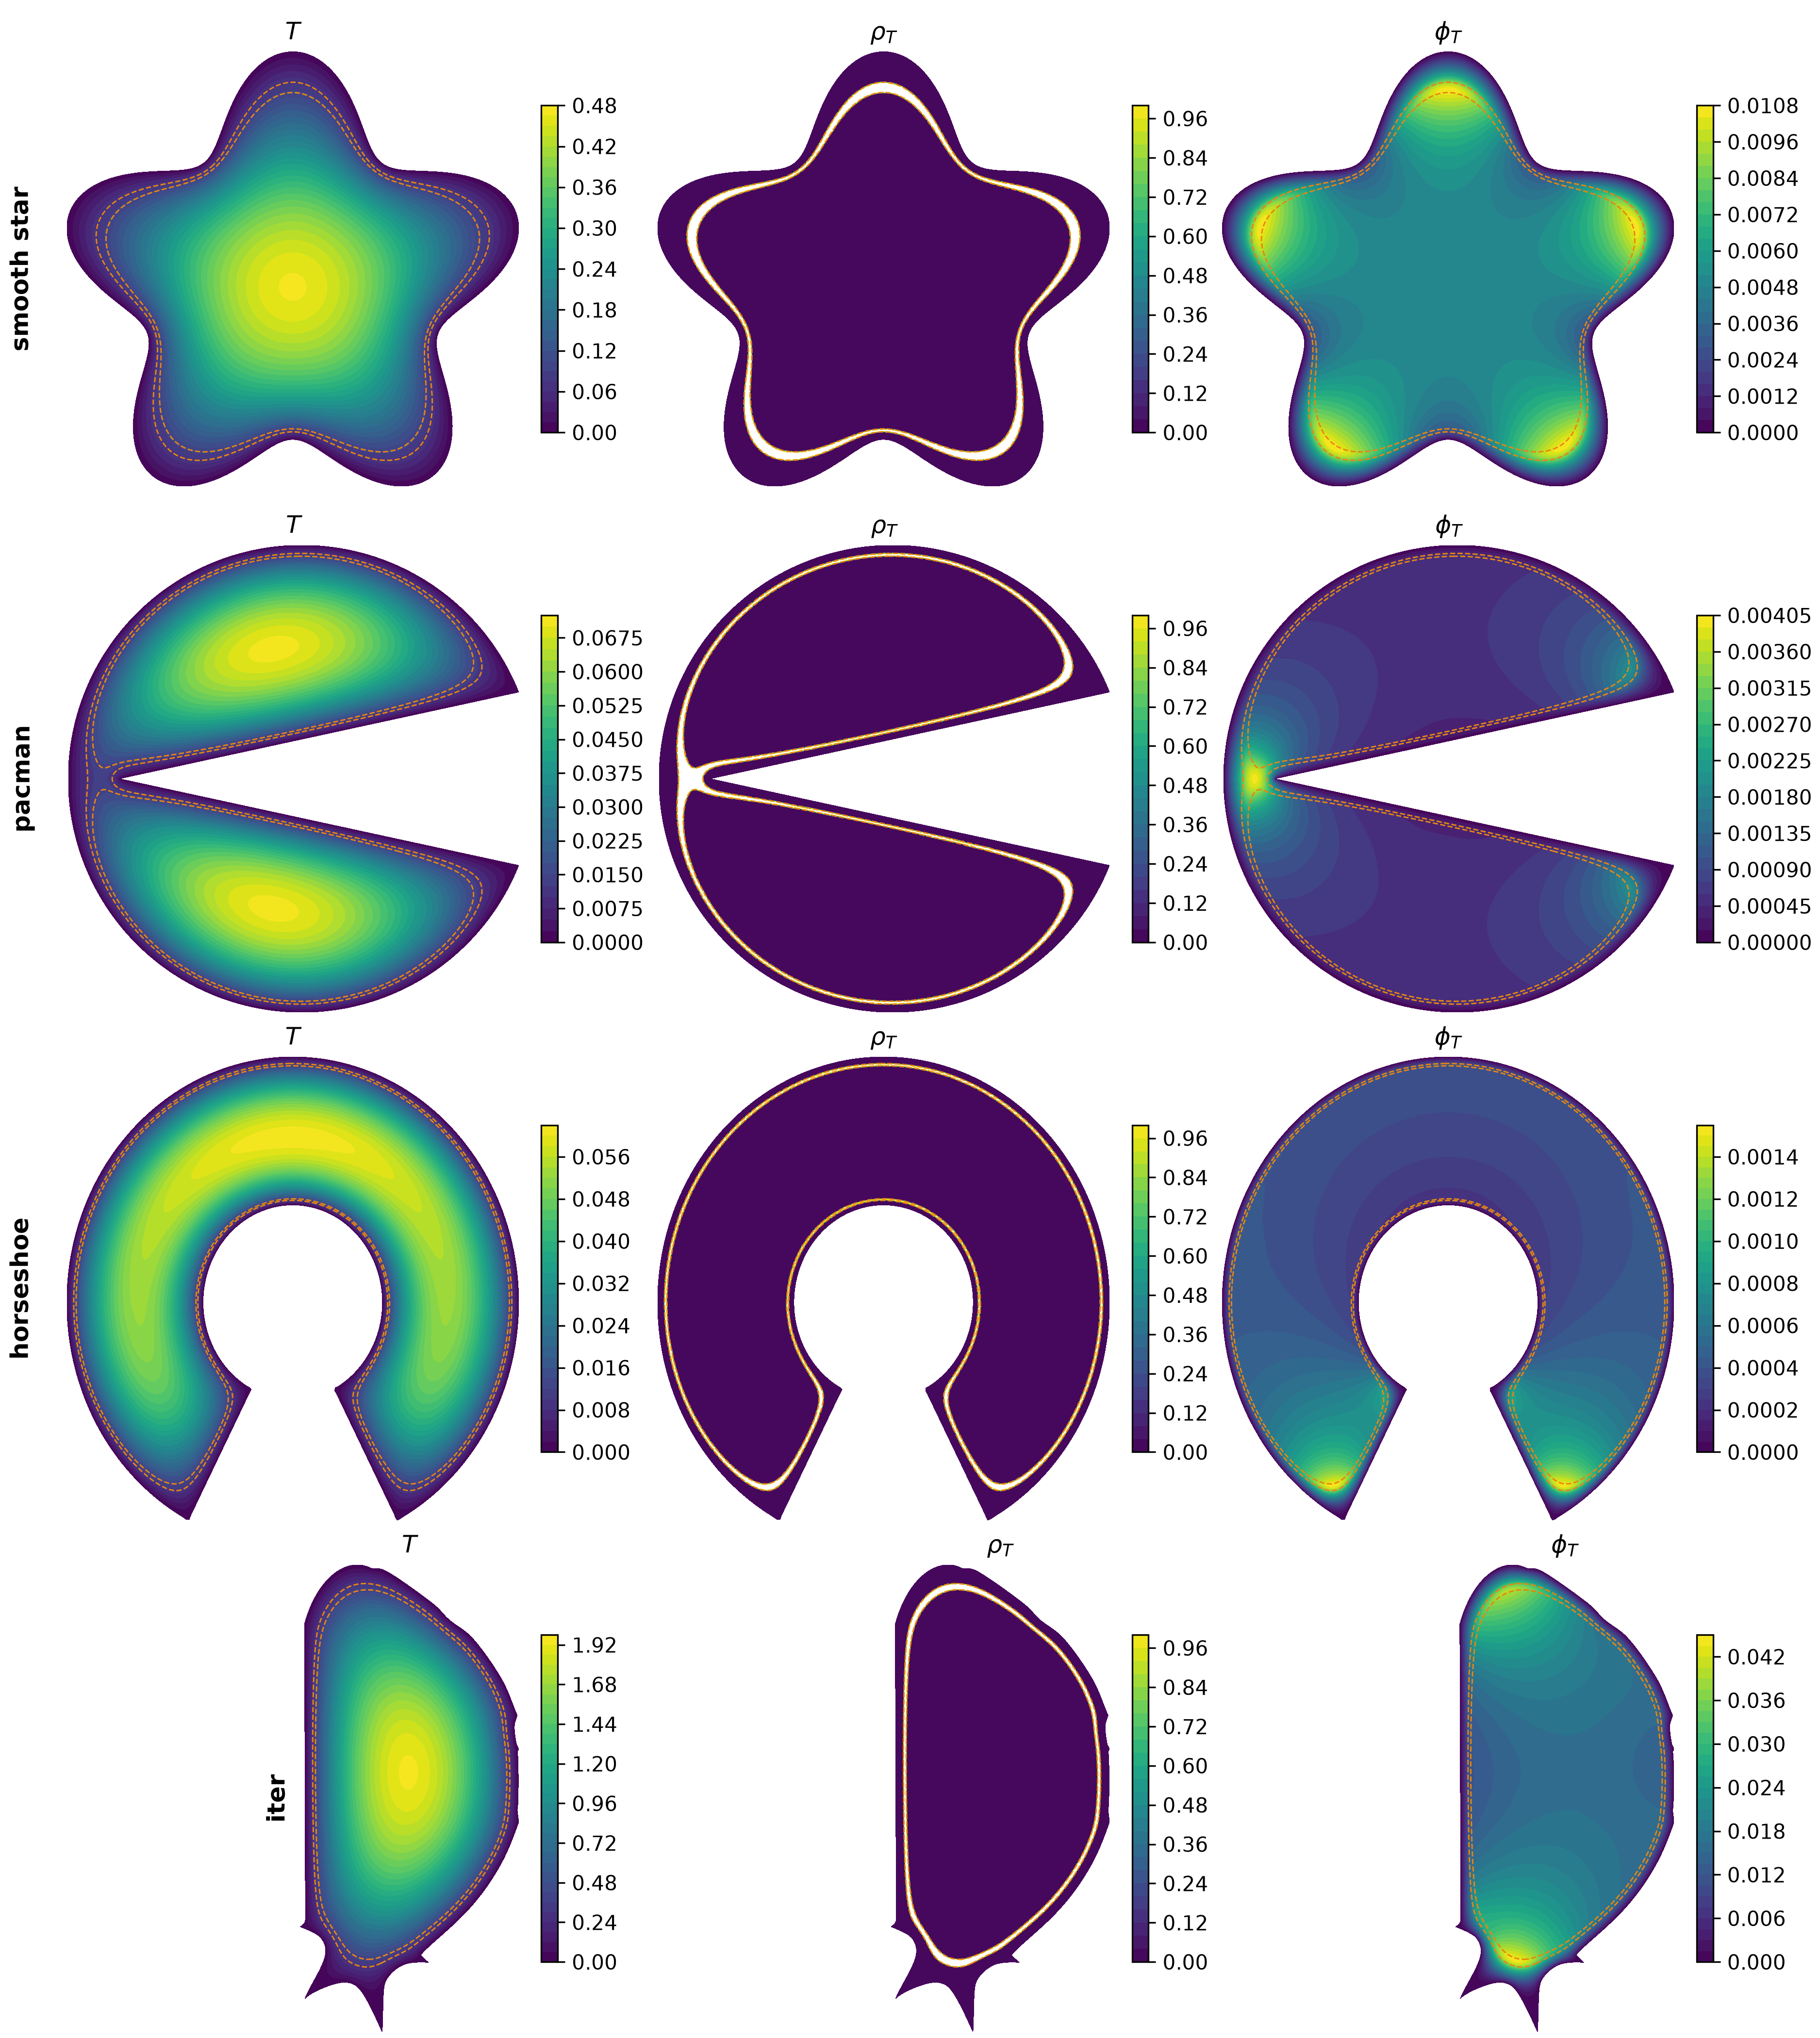
\includegraphics[width=0.88\linewidth]{figures/geometry_target_overview.png}
\caption{Canonical geometries, torsion fields, thin near-wall target bands at normalized torsion levels 0.15--0.20, and target potentials. Data status: actual.}
\label{fig:geometry-targets}
\end{figure}

\begin{figure}[tbp]
\centering
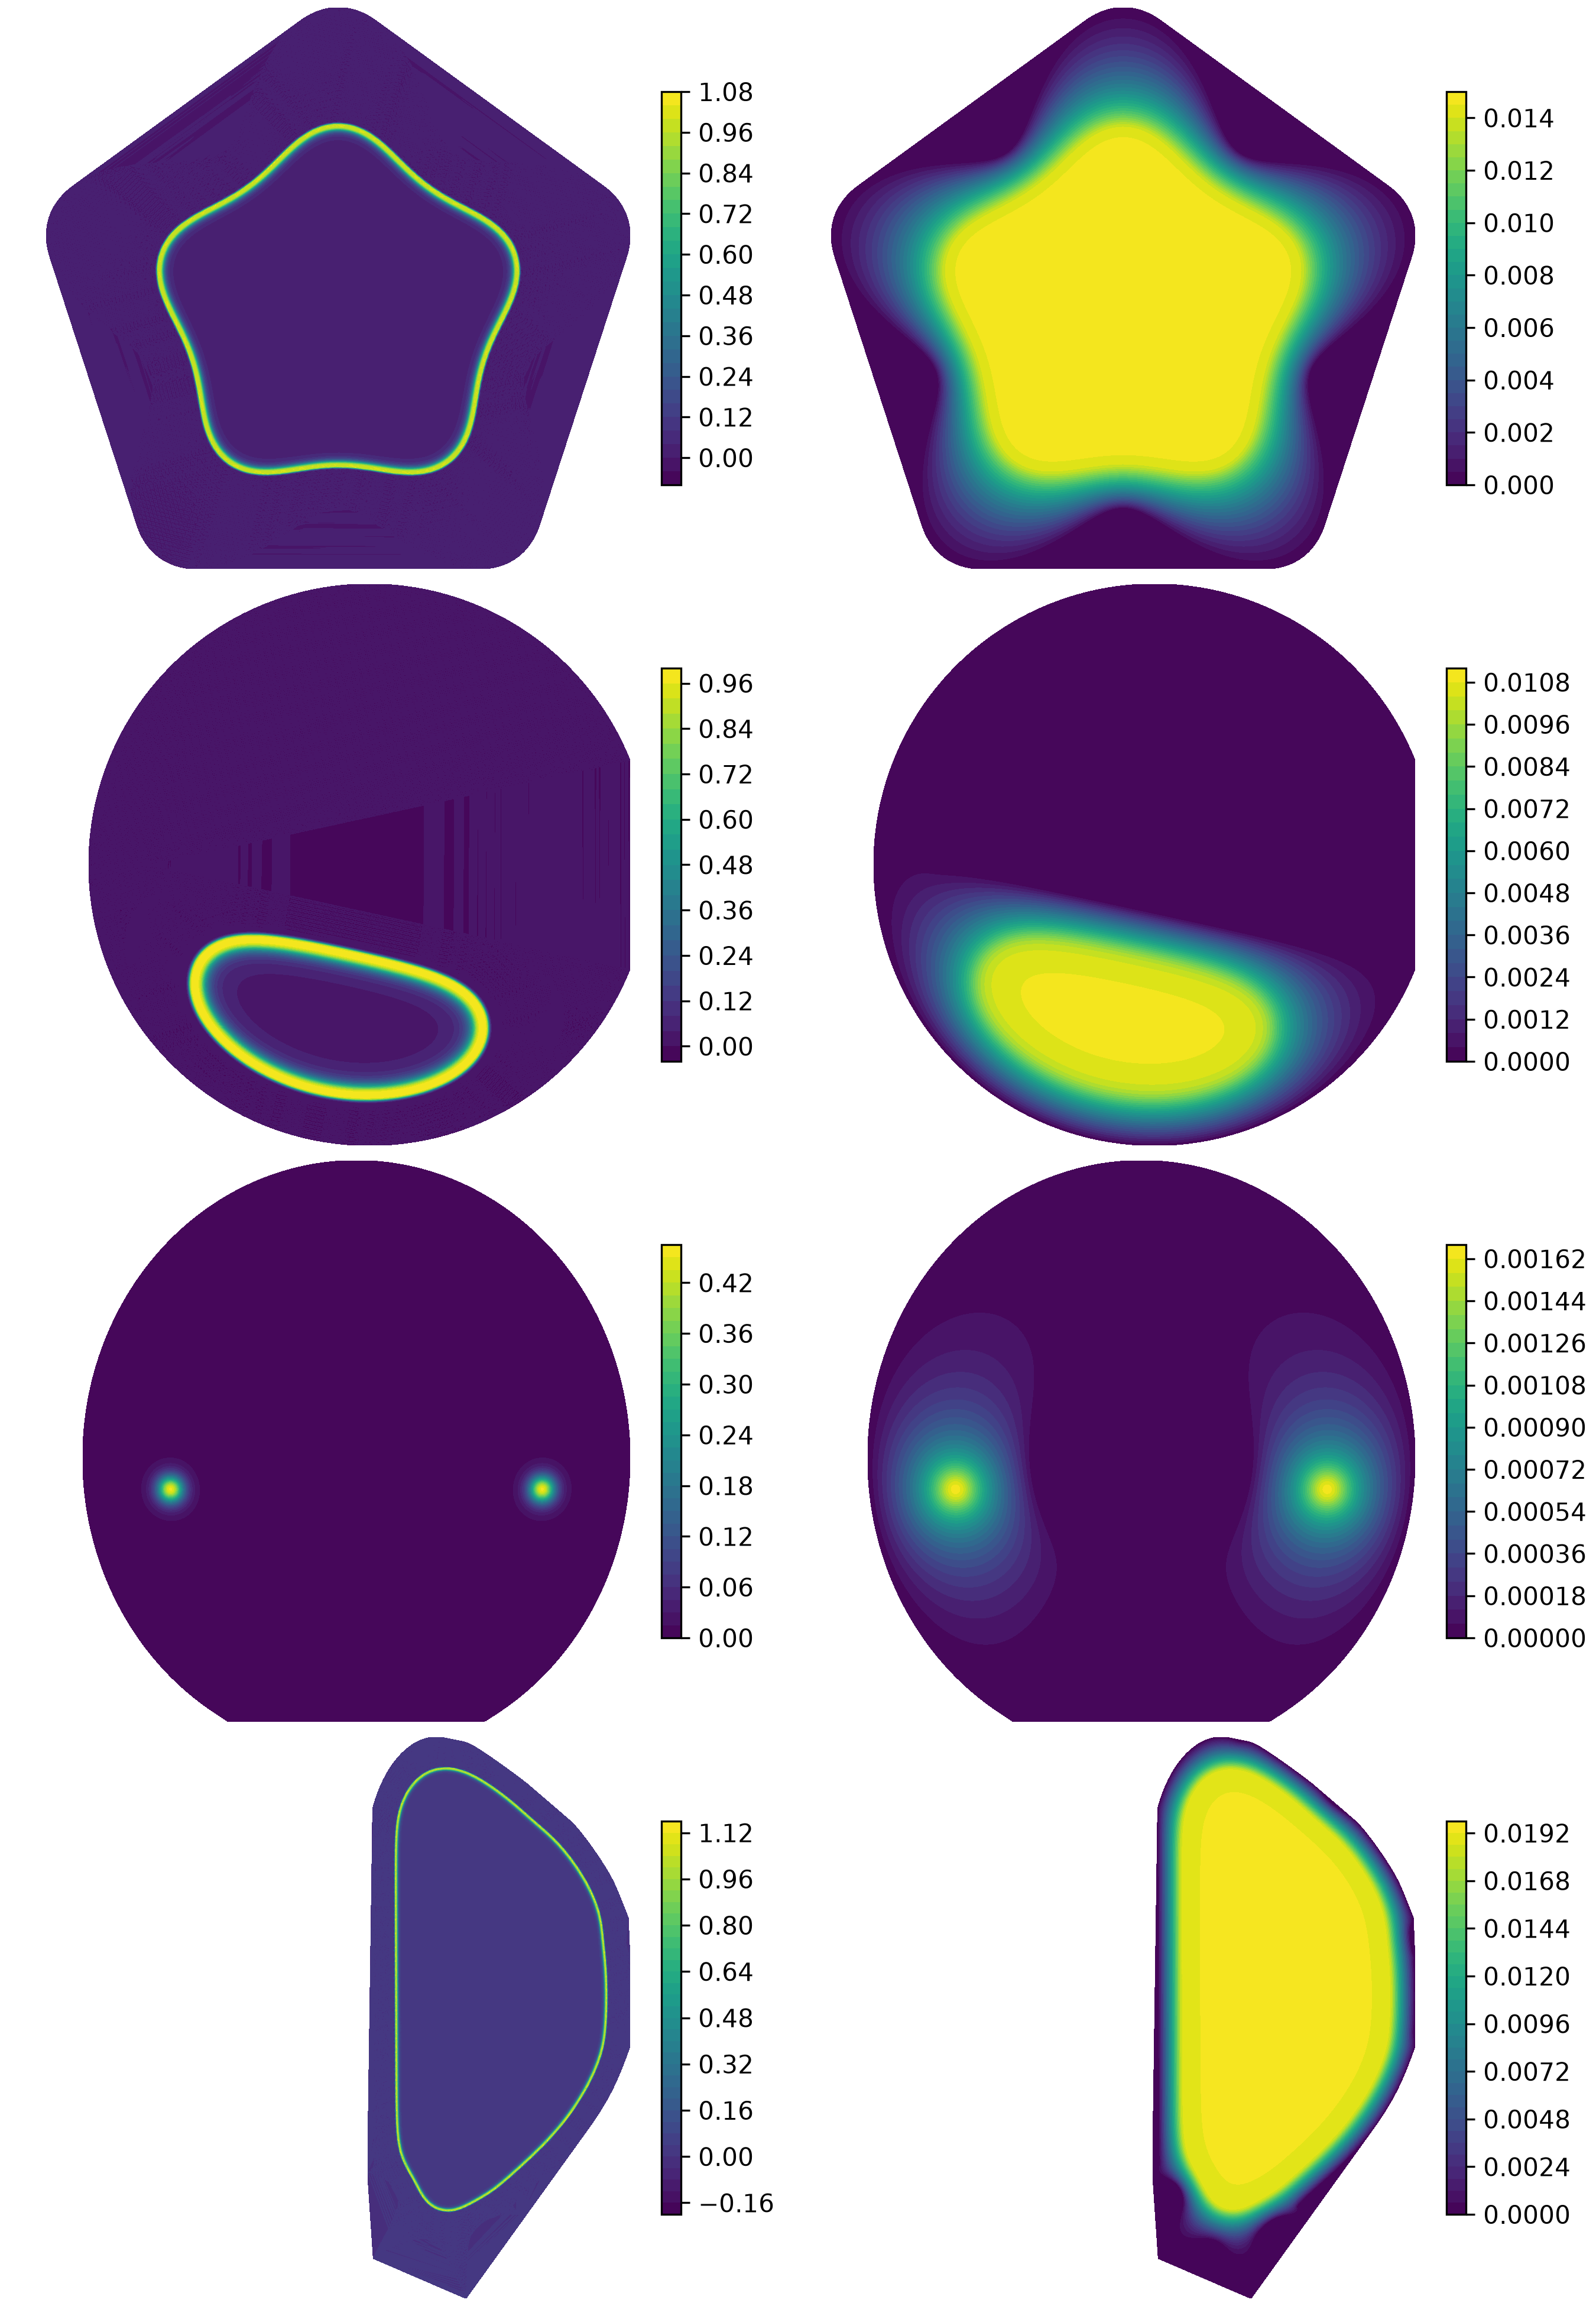
\includegraphics[width=0.88\linewidth]{figures/equilibrium_outcomes.png}
\caption{Equilibrium density and potential, with terminal failures retained. Data status: actual.}
\label{fig:equilibrium-outcomes}
\end{figure}

\begin{figure}[tbp]
\centering
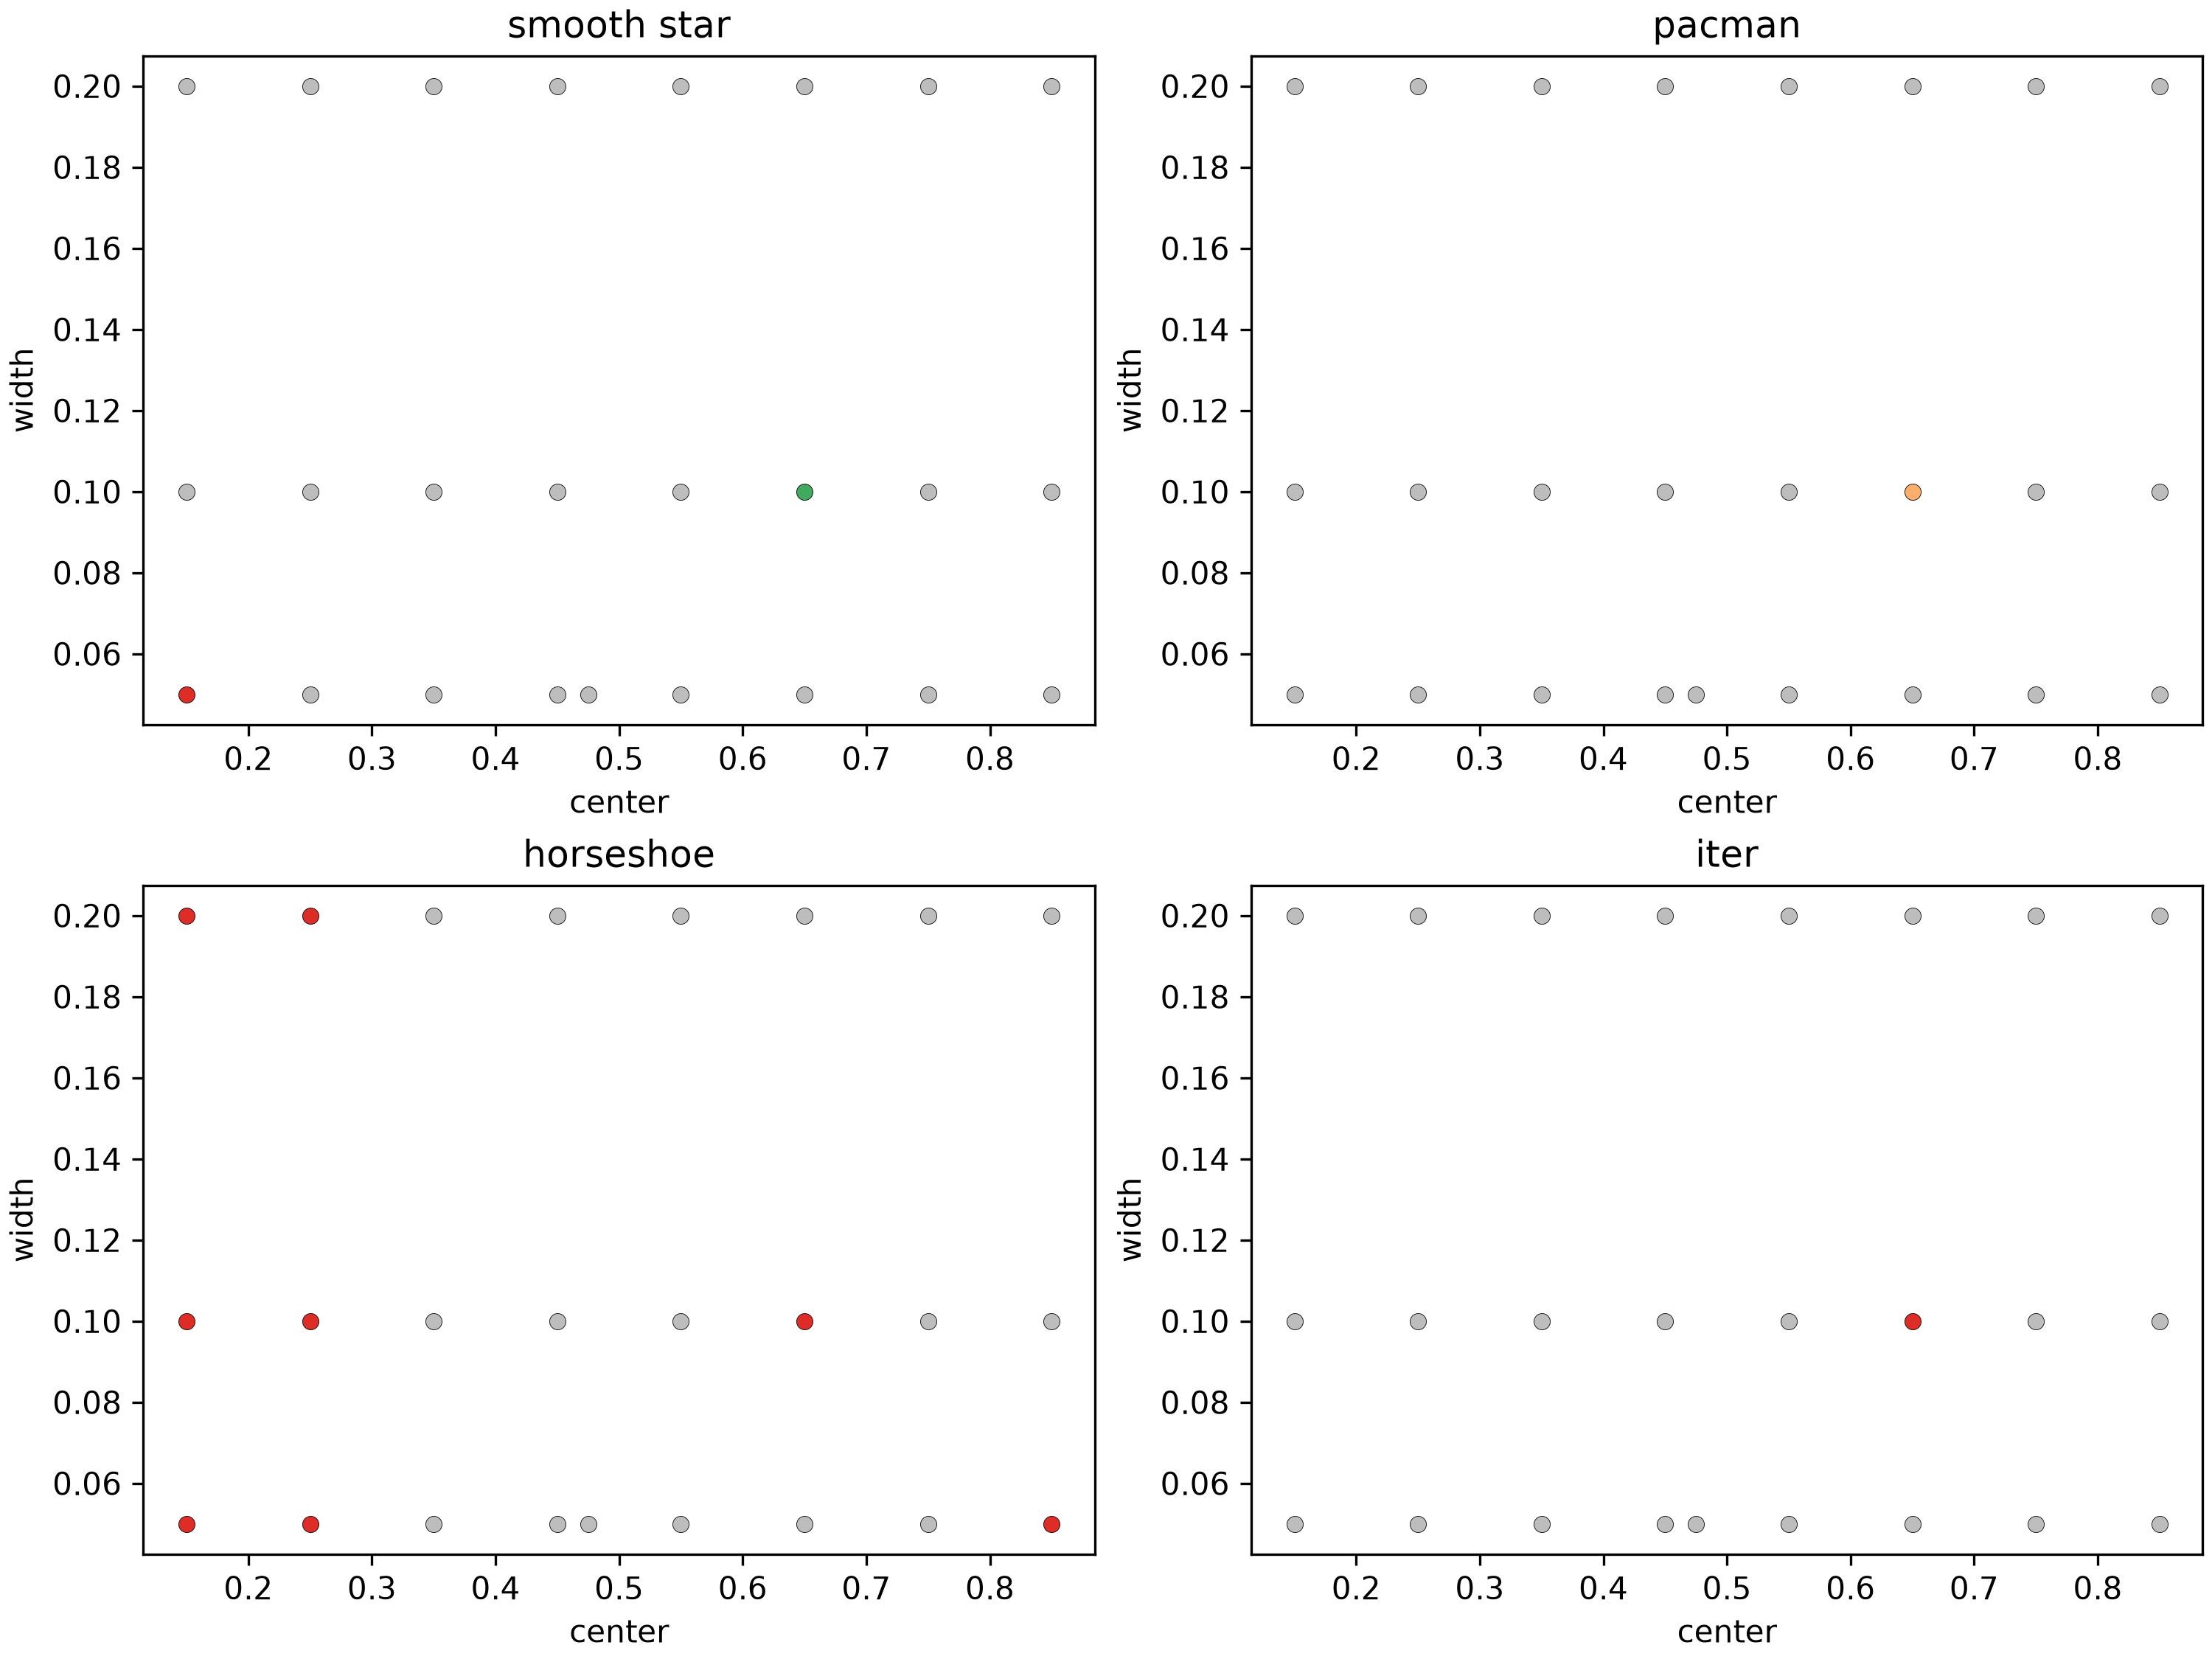
\includegraphics[width=0.88\linewidth]{figures/robustness_status_maps.png}
\caption{Torsion-level robustness status maps. Data status: partial.}
\label{fig:robustness}
\end{figure}

\begin{figure}[tbp]
\centering
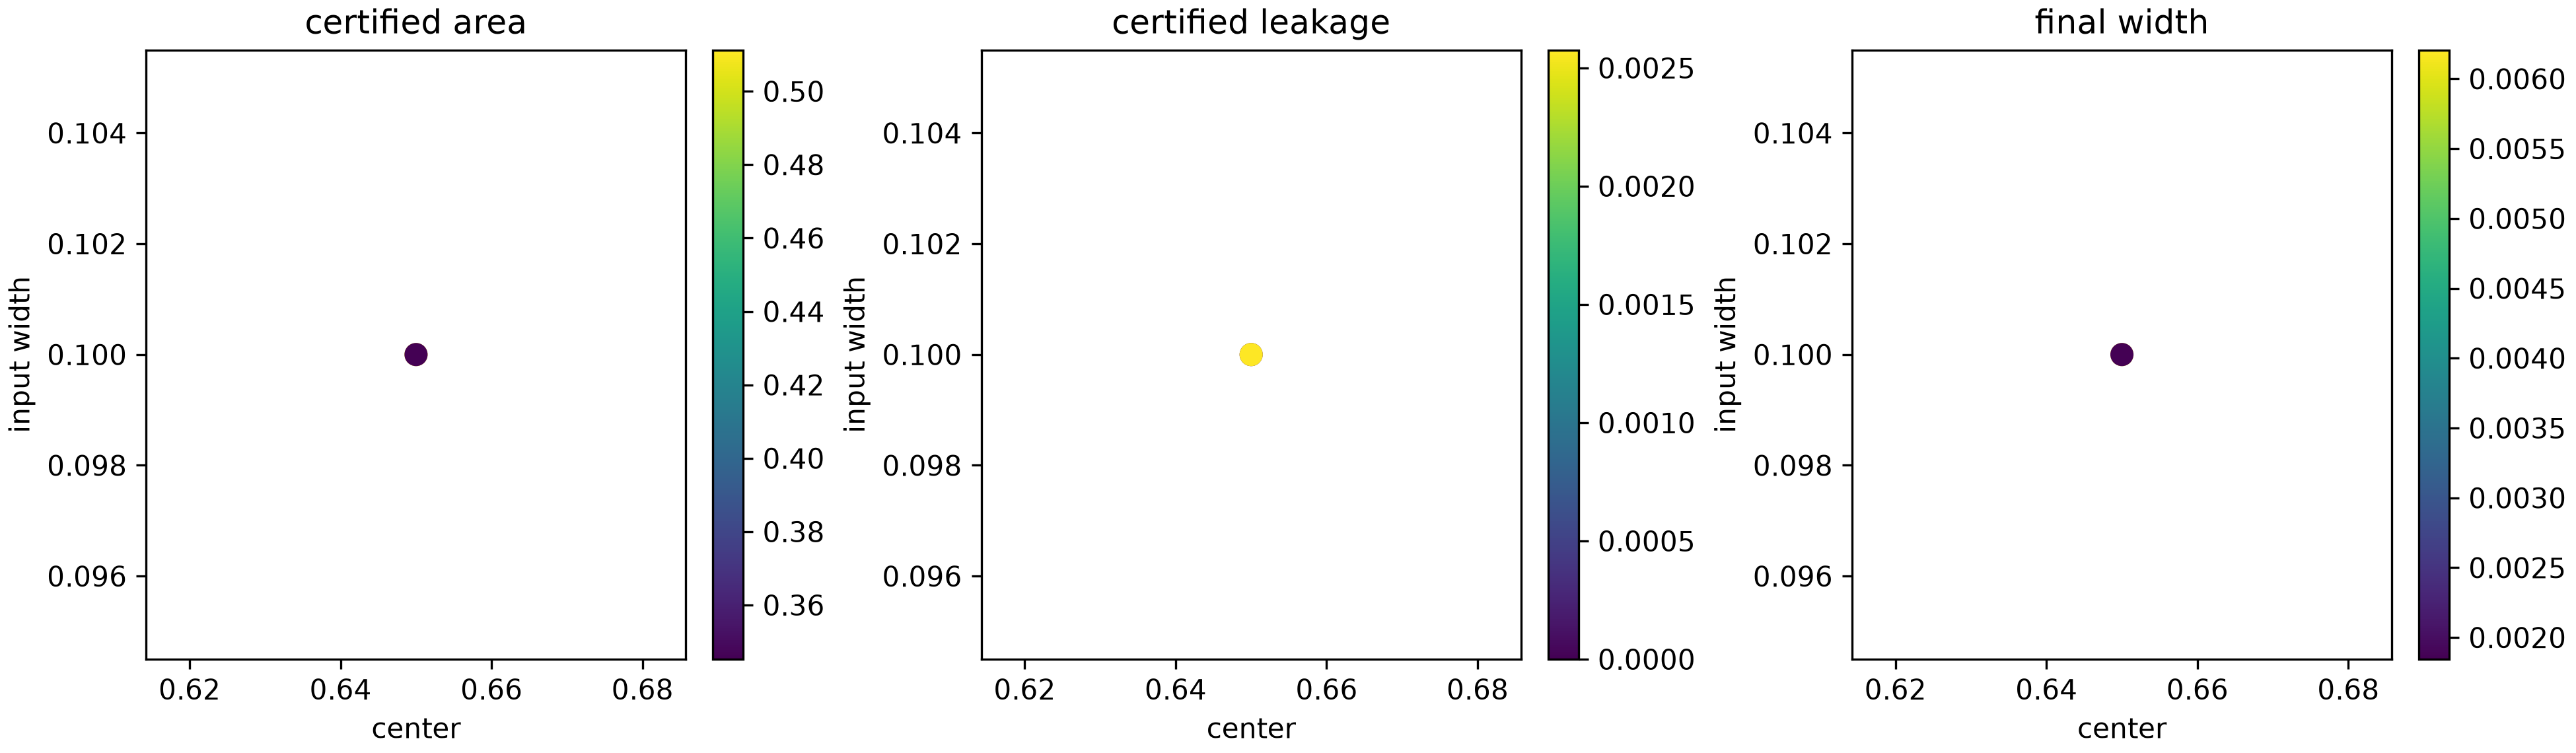
\includegraphics[width=0.88\linewidth]{figures/robustness_metrics_summary.png}
\caption{Certified area, leakage, and final threshold width. Data status: partial.}
\label{fig:robustness-metrics}
\end{figure}

\begin{figure}[tbp]
\centering
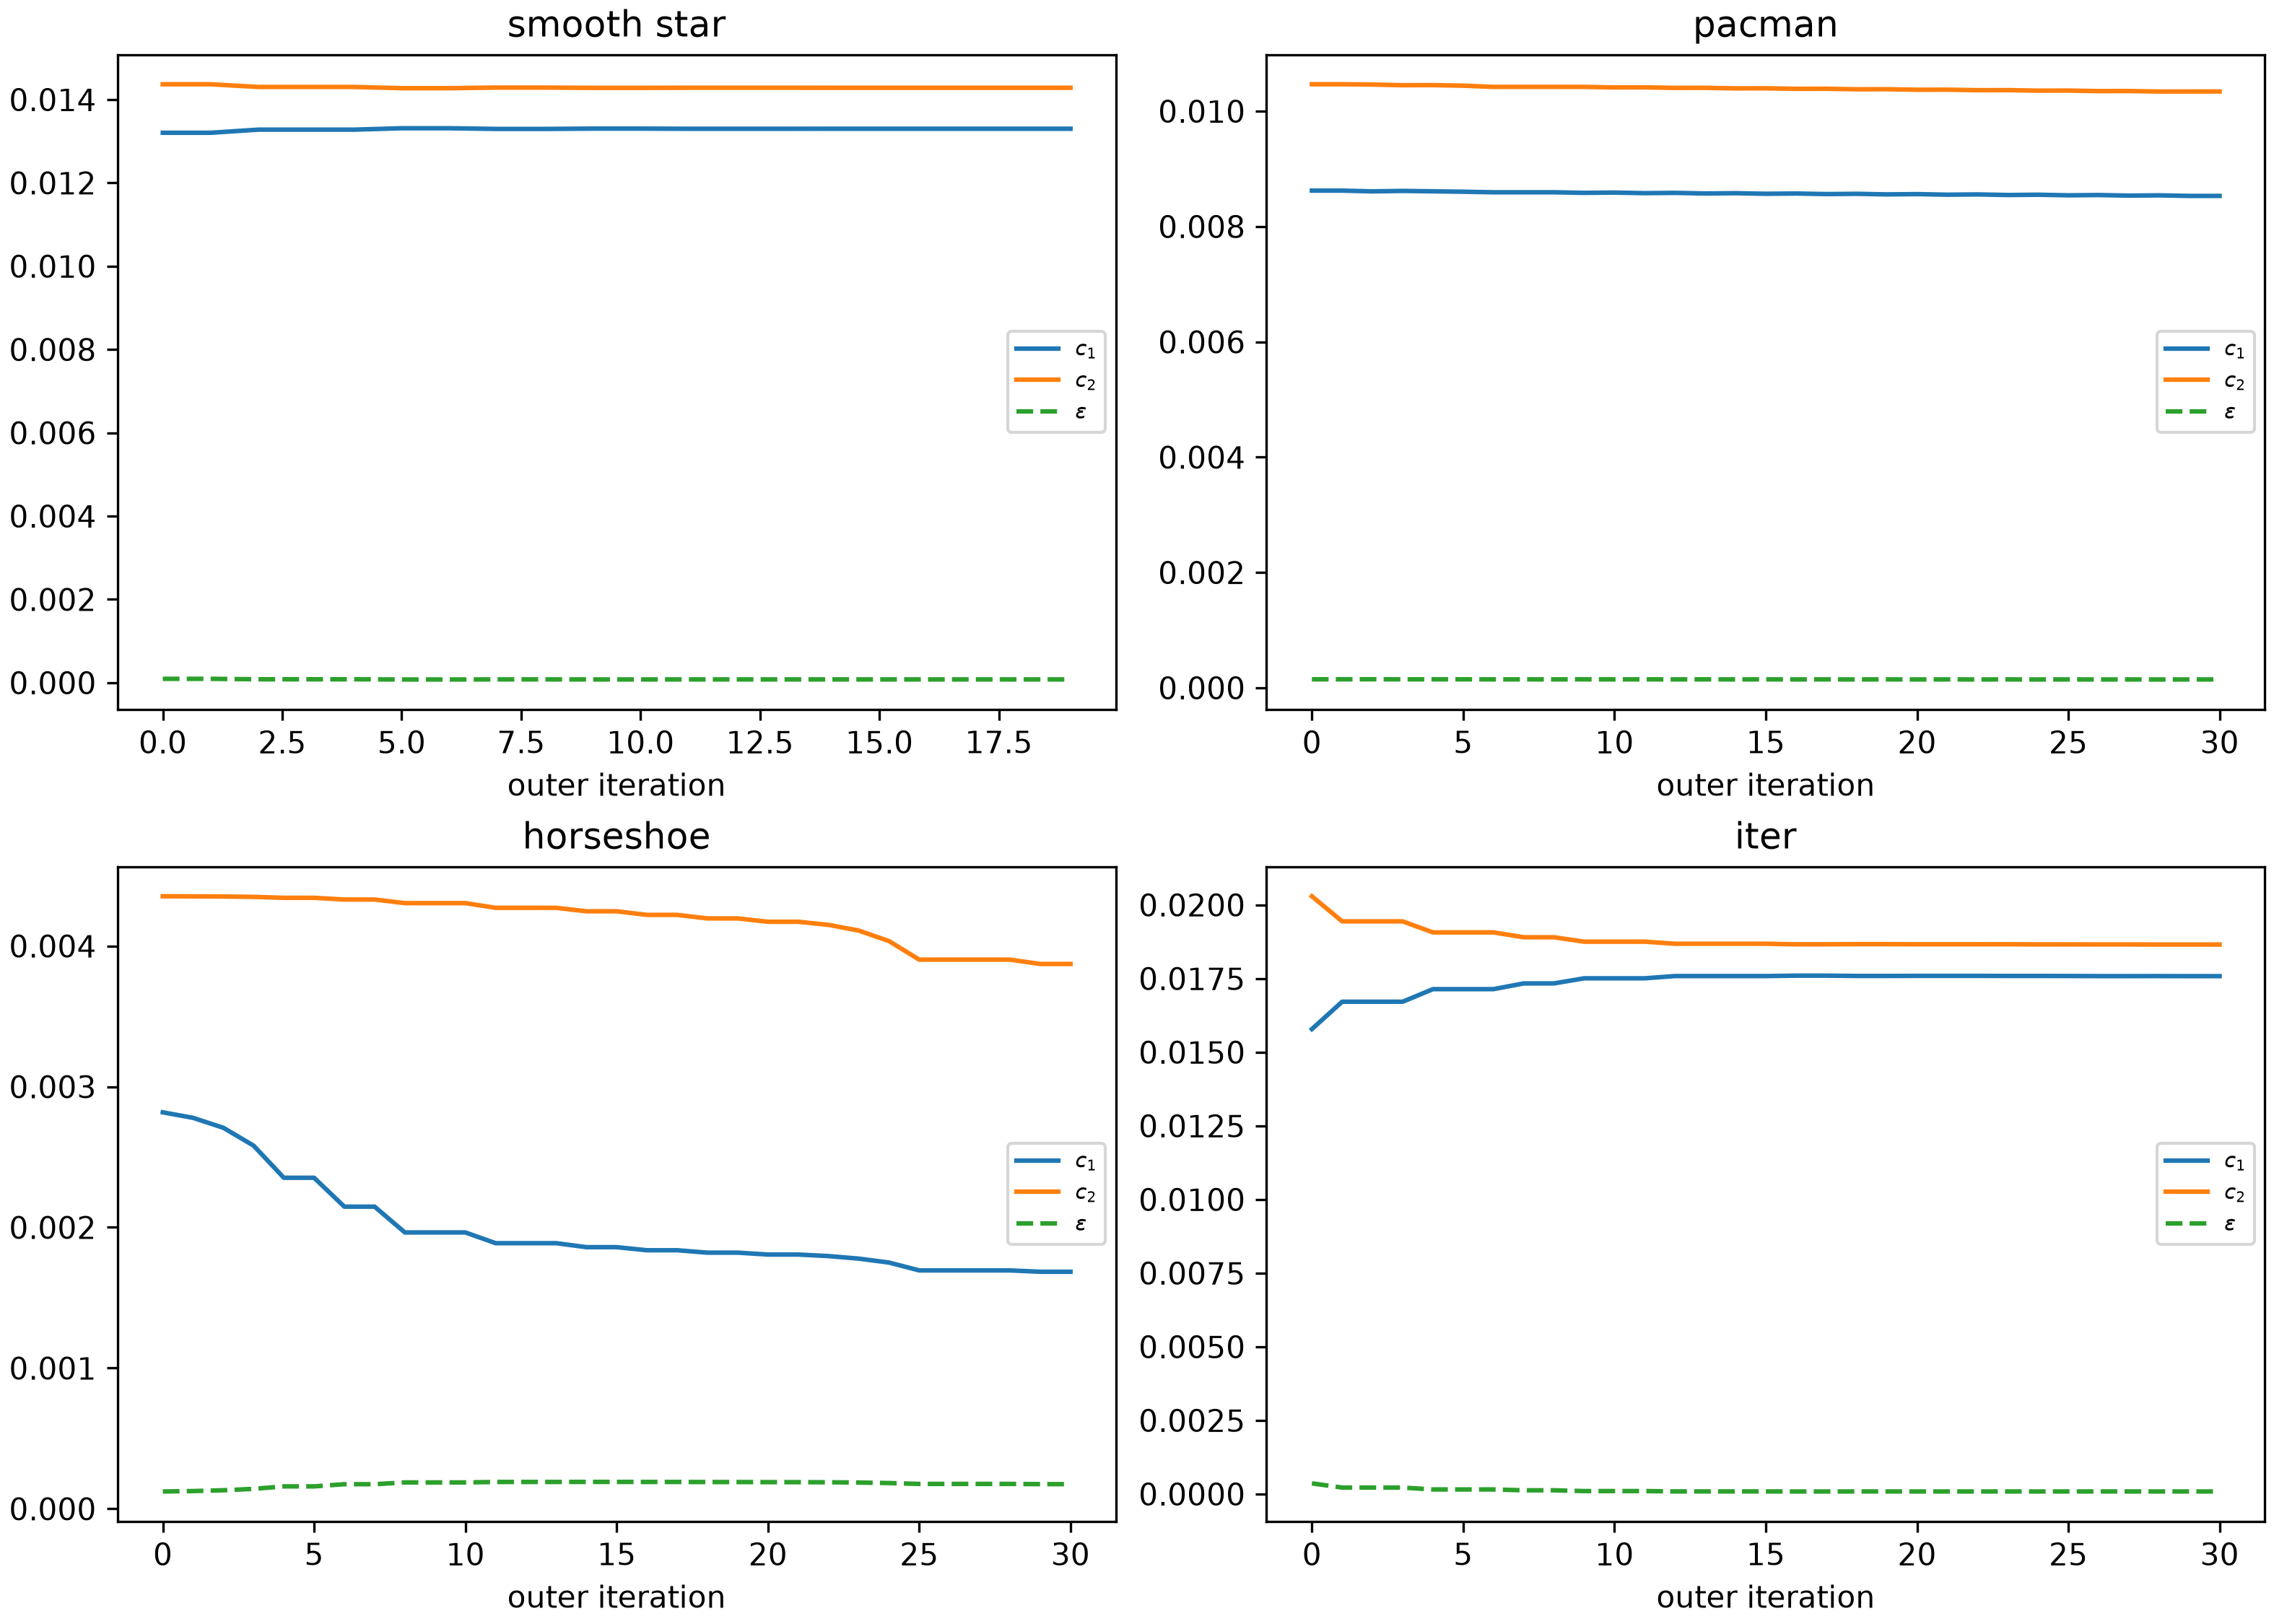
\includegraphics[width=0.88\linewidth]{figures/threshold_evolution.png}
\caption{Threshold, band-width, smoothing, and discrepancy evolution. Data status: actual.}
\label{fig:threshold-history}
\end{figure}

\begin{figure}[tbp]
\centering
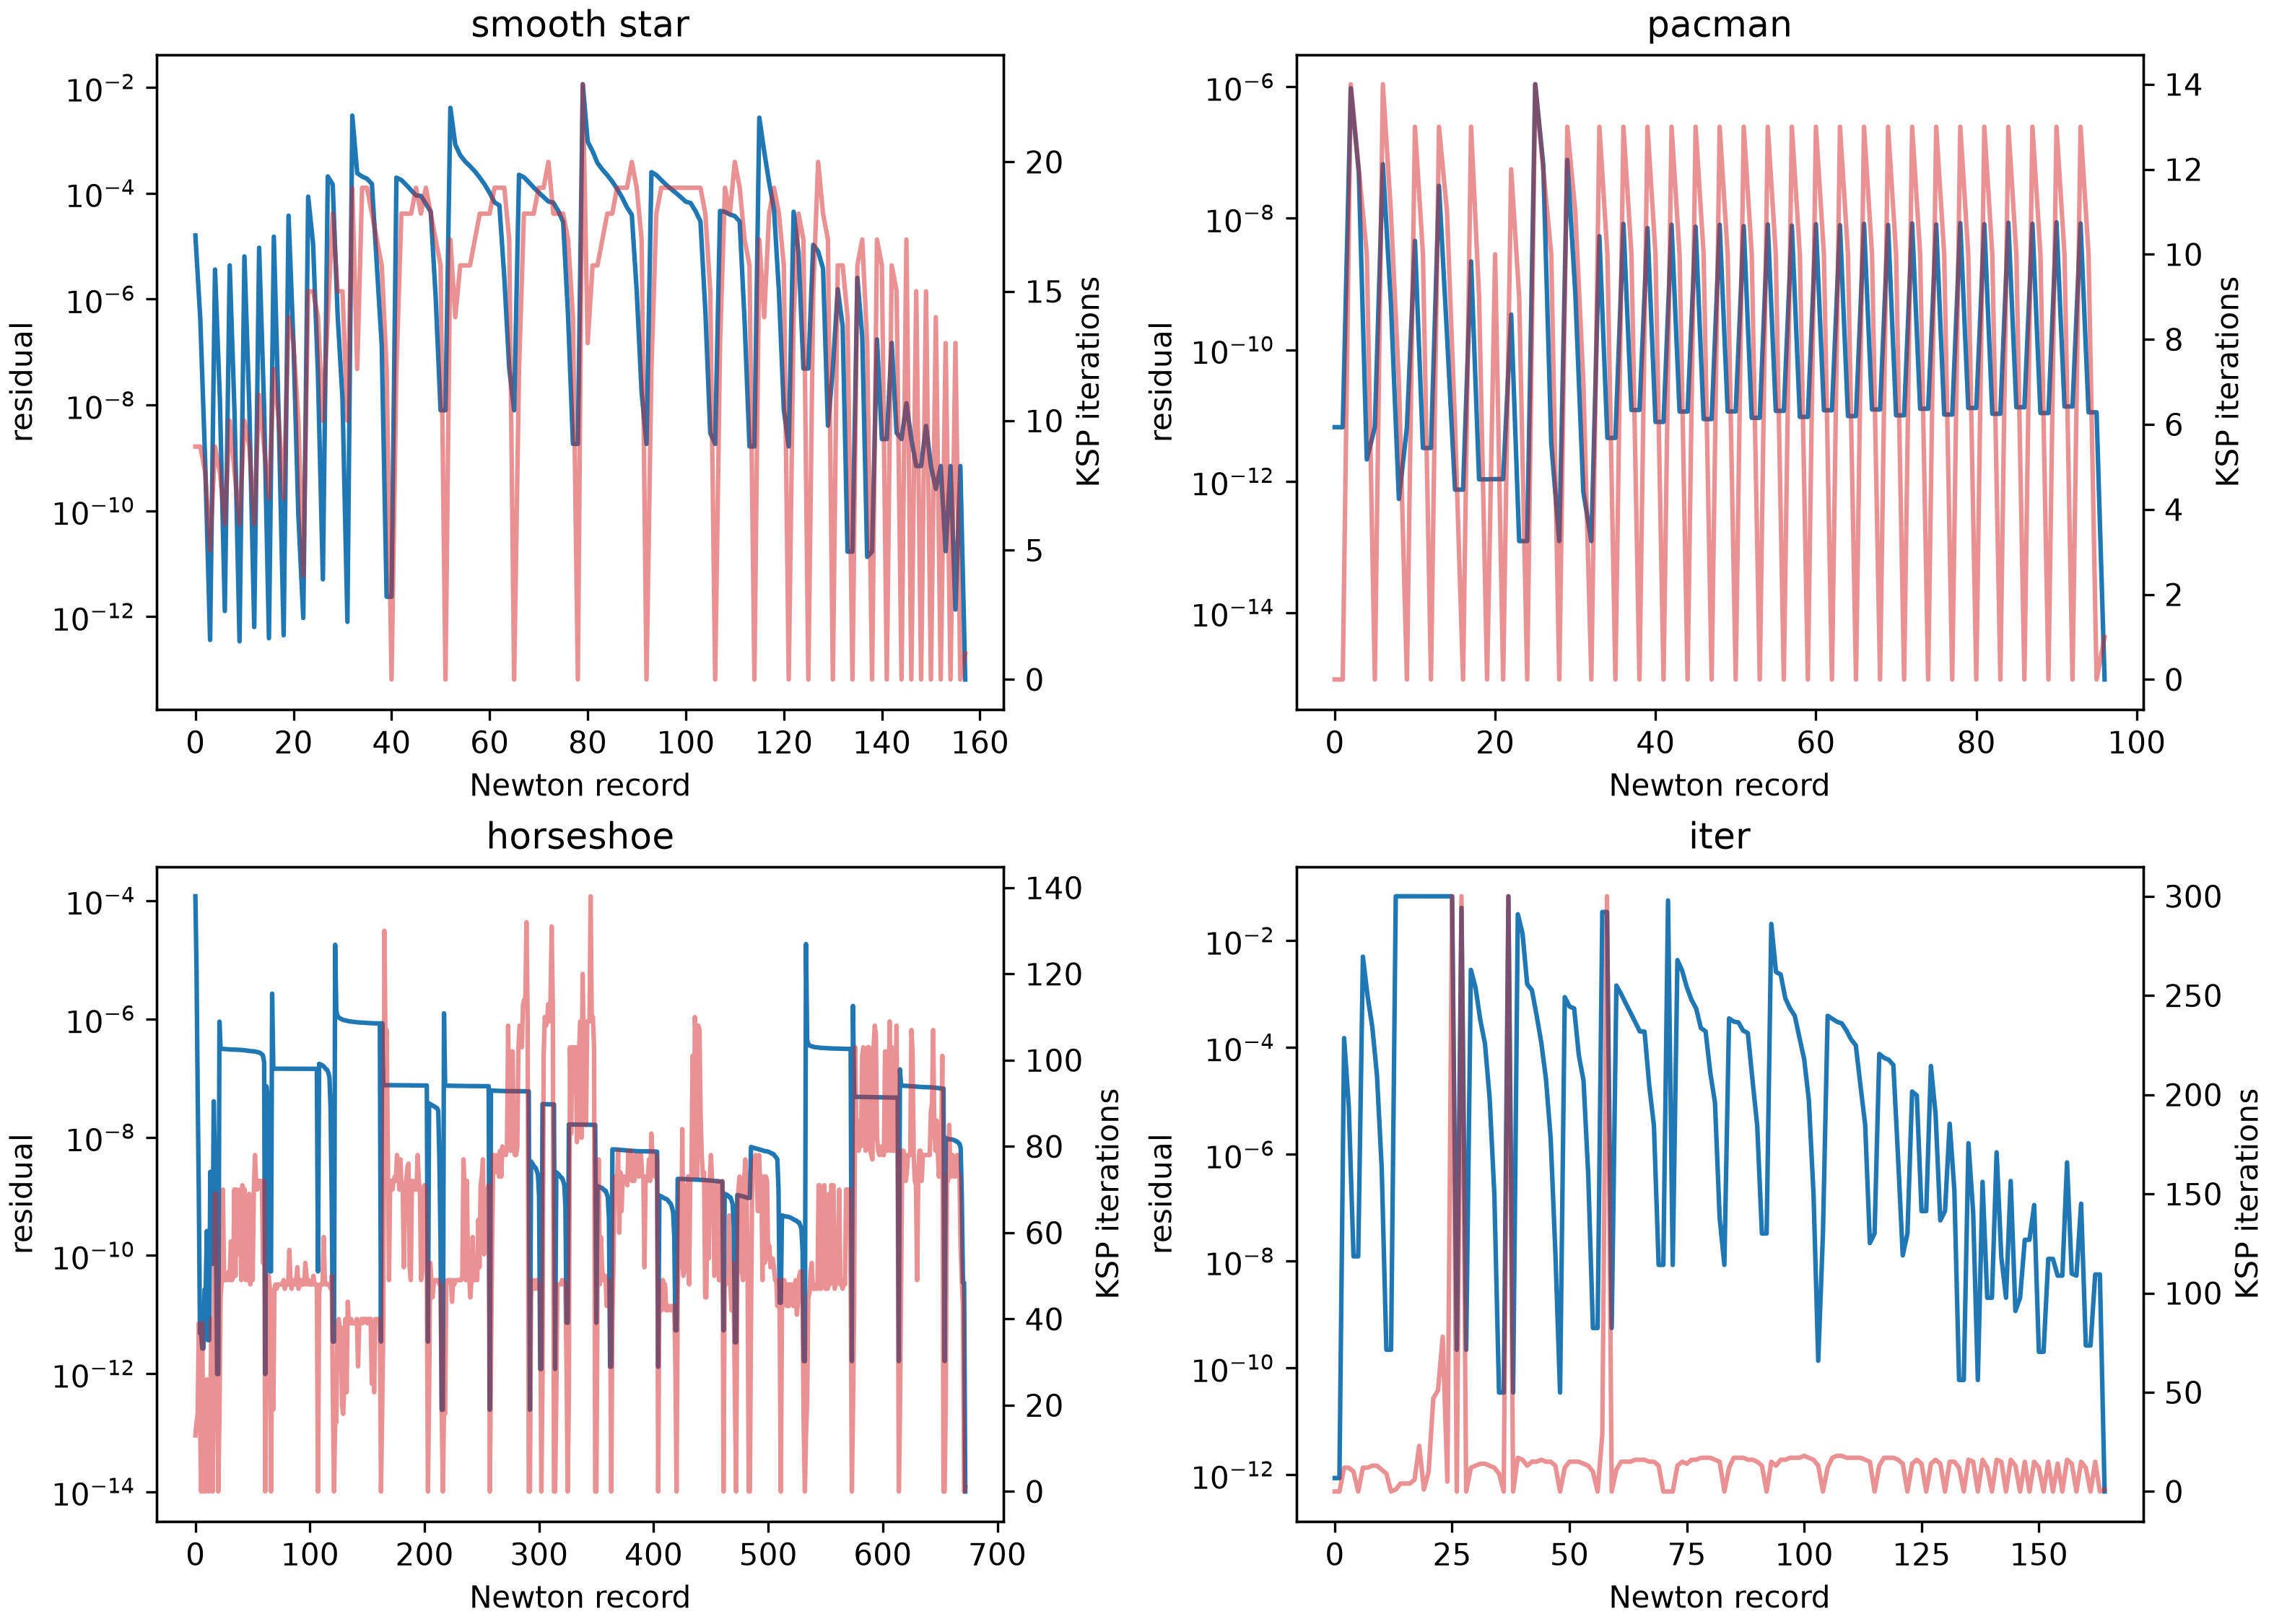
\includegraphics[width=0.88\linewidth]{figures/newton_ksp_diagnostics.png}
\caption{Newton residual and Krylov work. Data status: actual.}
\label{fig:newton-ksp}
\end{figure}

\begin{figure}[tbp]
\centering
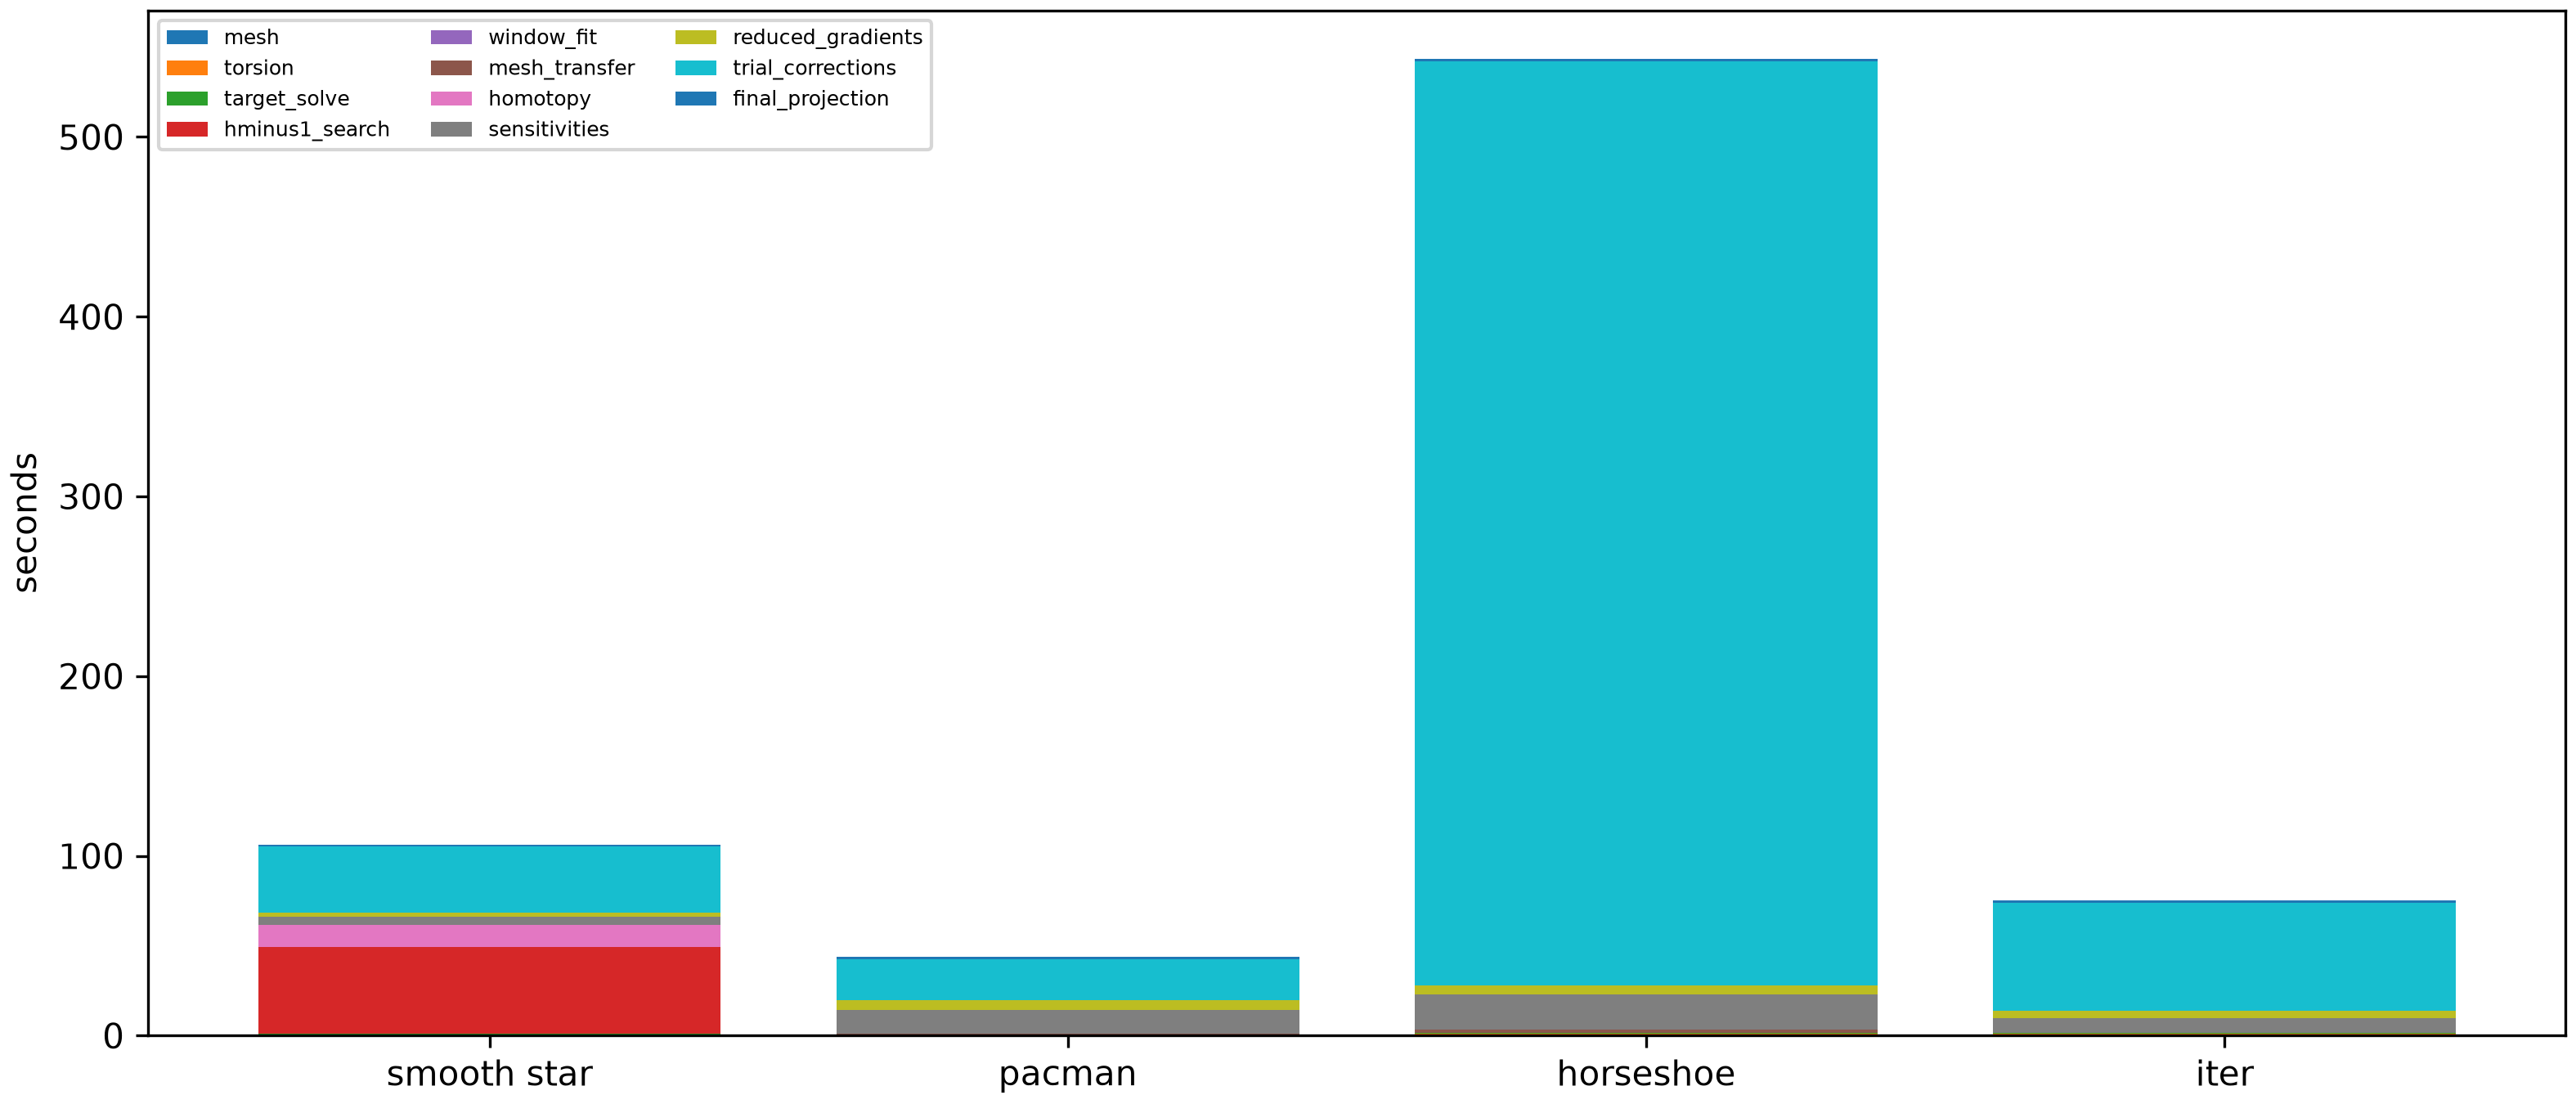
\includegraphics[width=0.88\linewidth]{figures/phase_timing_breakdown.png}
\caption{Initialization, homotopy, optimization, and projection time. Data status: actual.}
\label{fig:phase-timing}
\end{figure}

\begin{figure}[tbp]
\centering
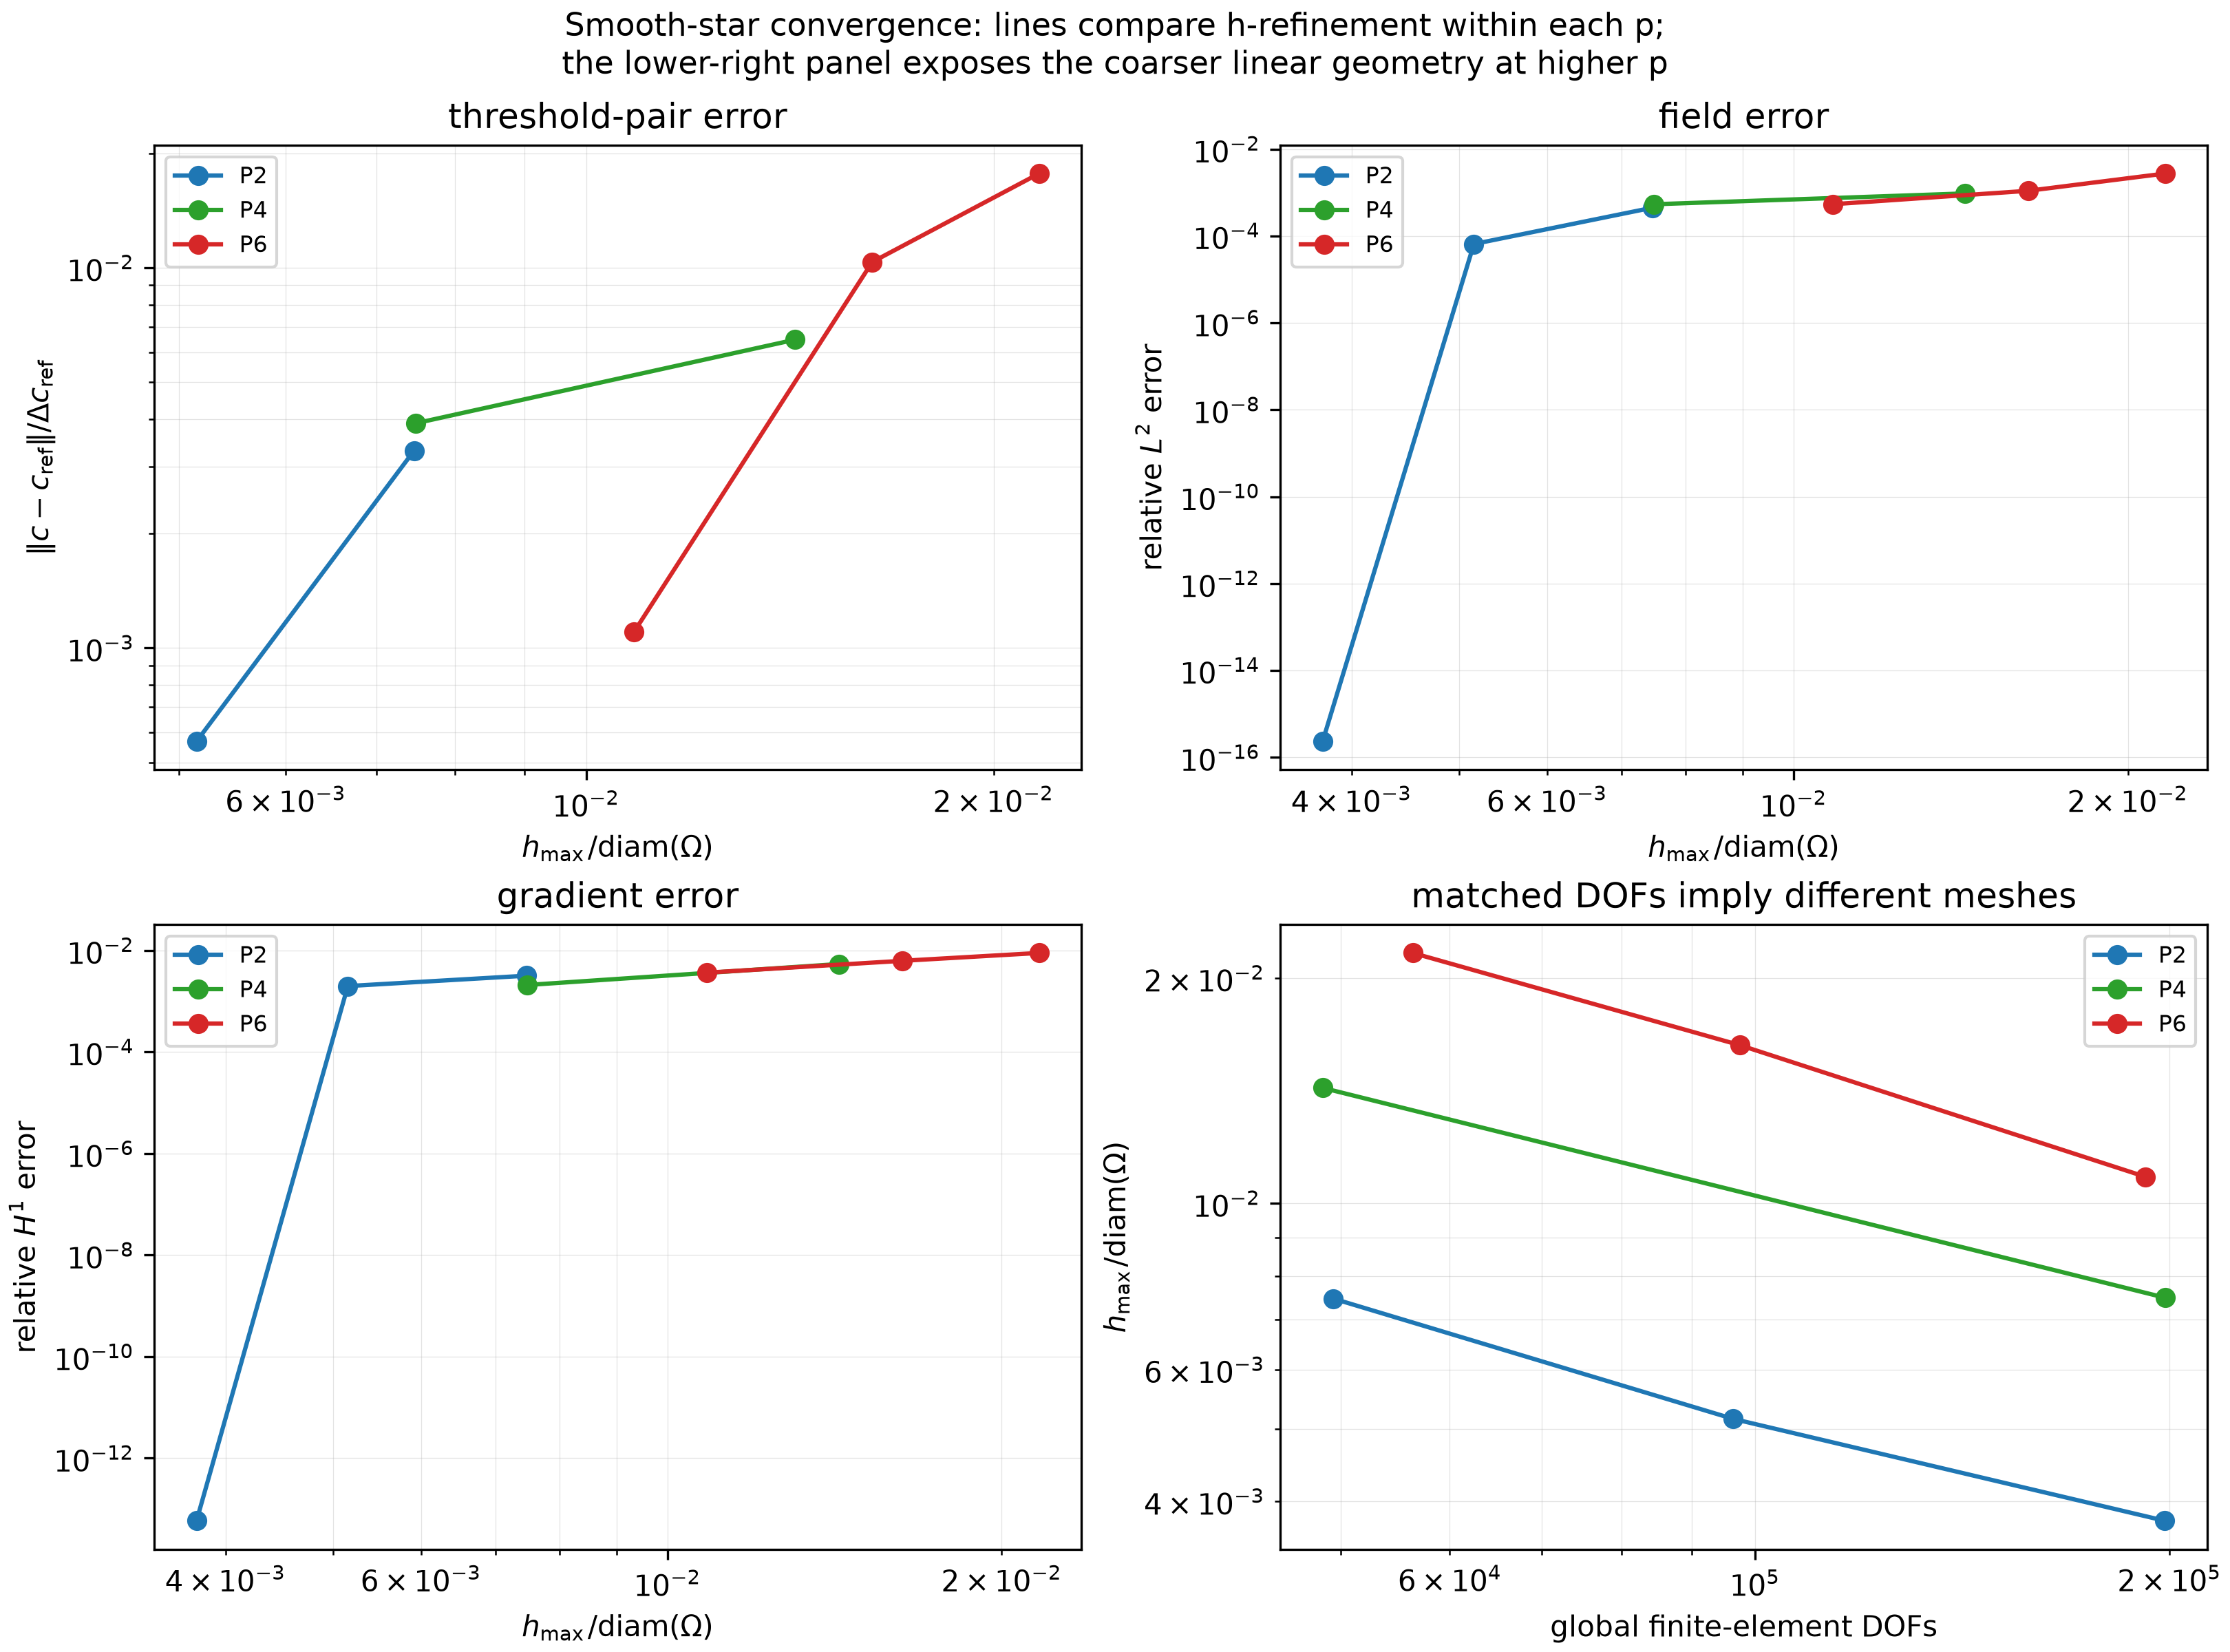
\includegraphics[width=0.88\linewidth]{figures/hp_convergence_summary.png}
\caption{Smooth-star h-convergence within P2, P4, and P6, with the matched-DOF mesh sizes shown explicitly. Higher p is not intrinsically less accurate; at fixed global DOFs it currently uses a much coarser linear boundary mesh. Data status: actual.}
\label{fig:hp-convergence}
\end{figure}

\clearpage

\begin{figure}[tbp]
\centering
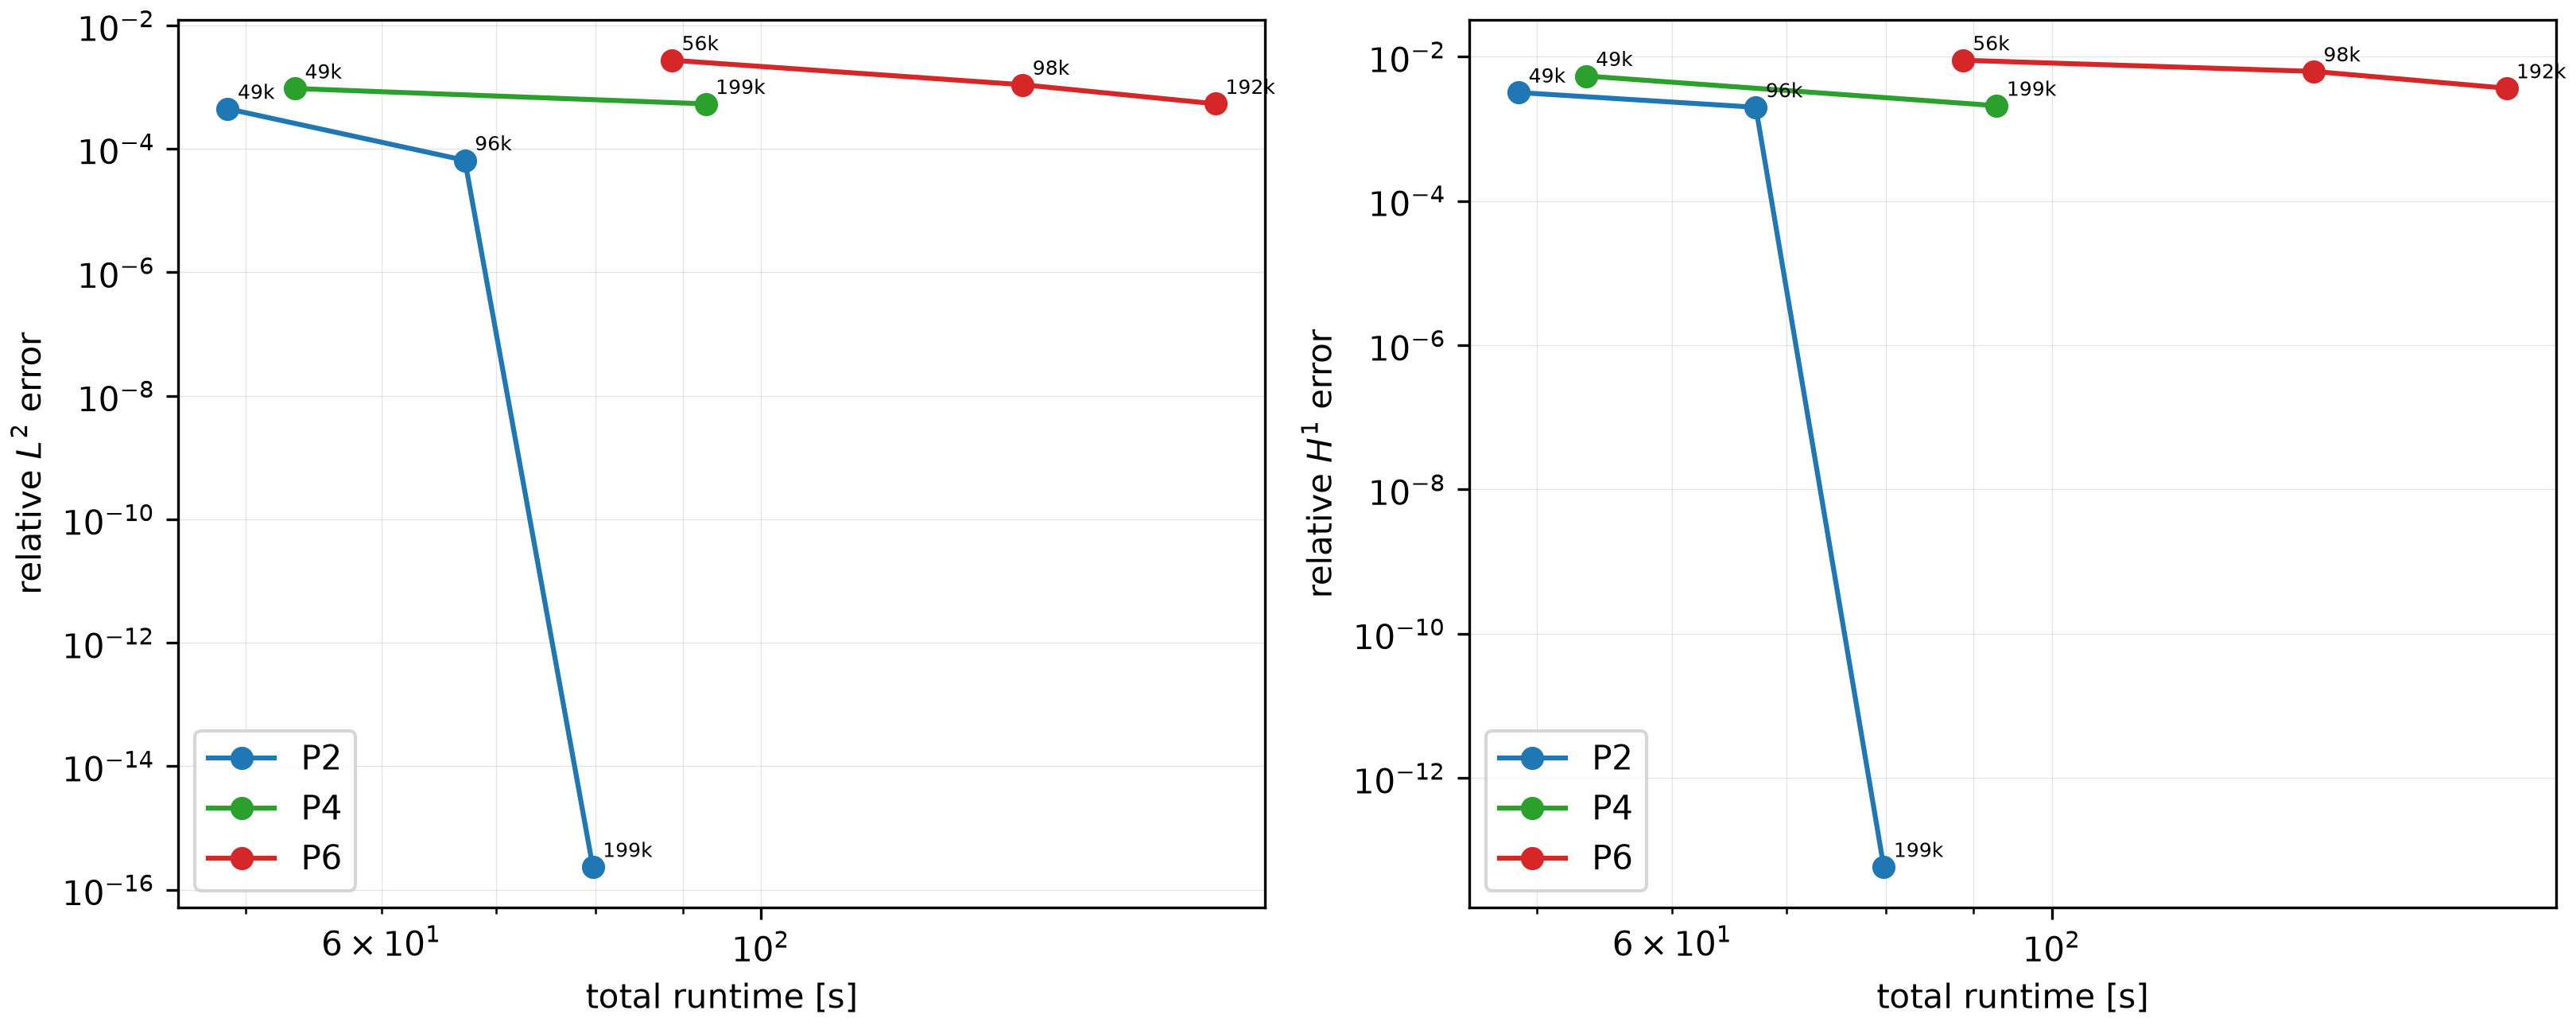
\includegraphics[width=0.88\linewidth]{figures/matched_cost_accuracy.png}
\caption{Relative field errors against runtime; labels give global DOFs. Data status: actual.}
\label{fig:matched-cost}
\end{figure}

\begin{figure}[tbp]
\centering
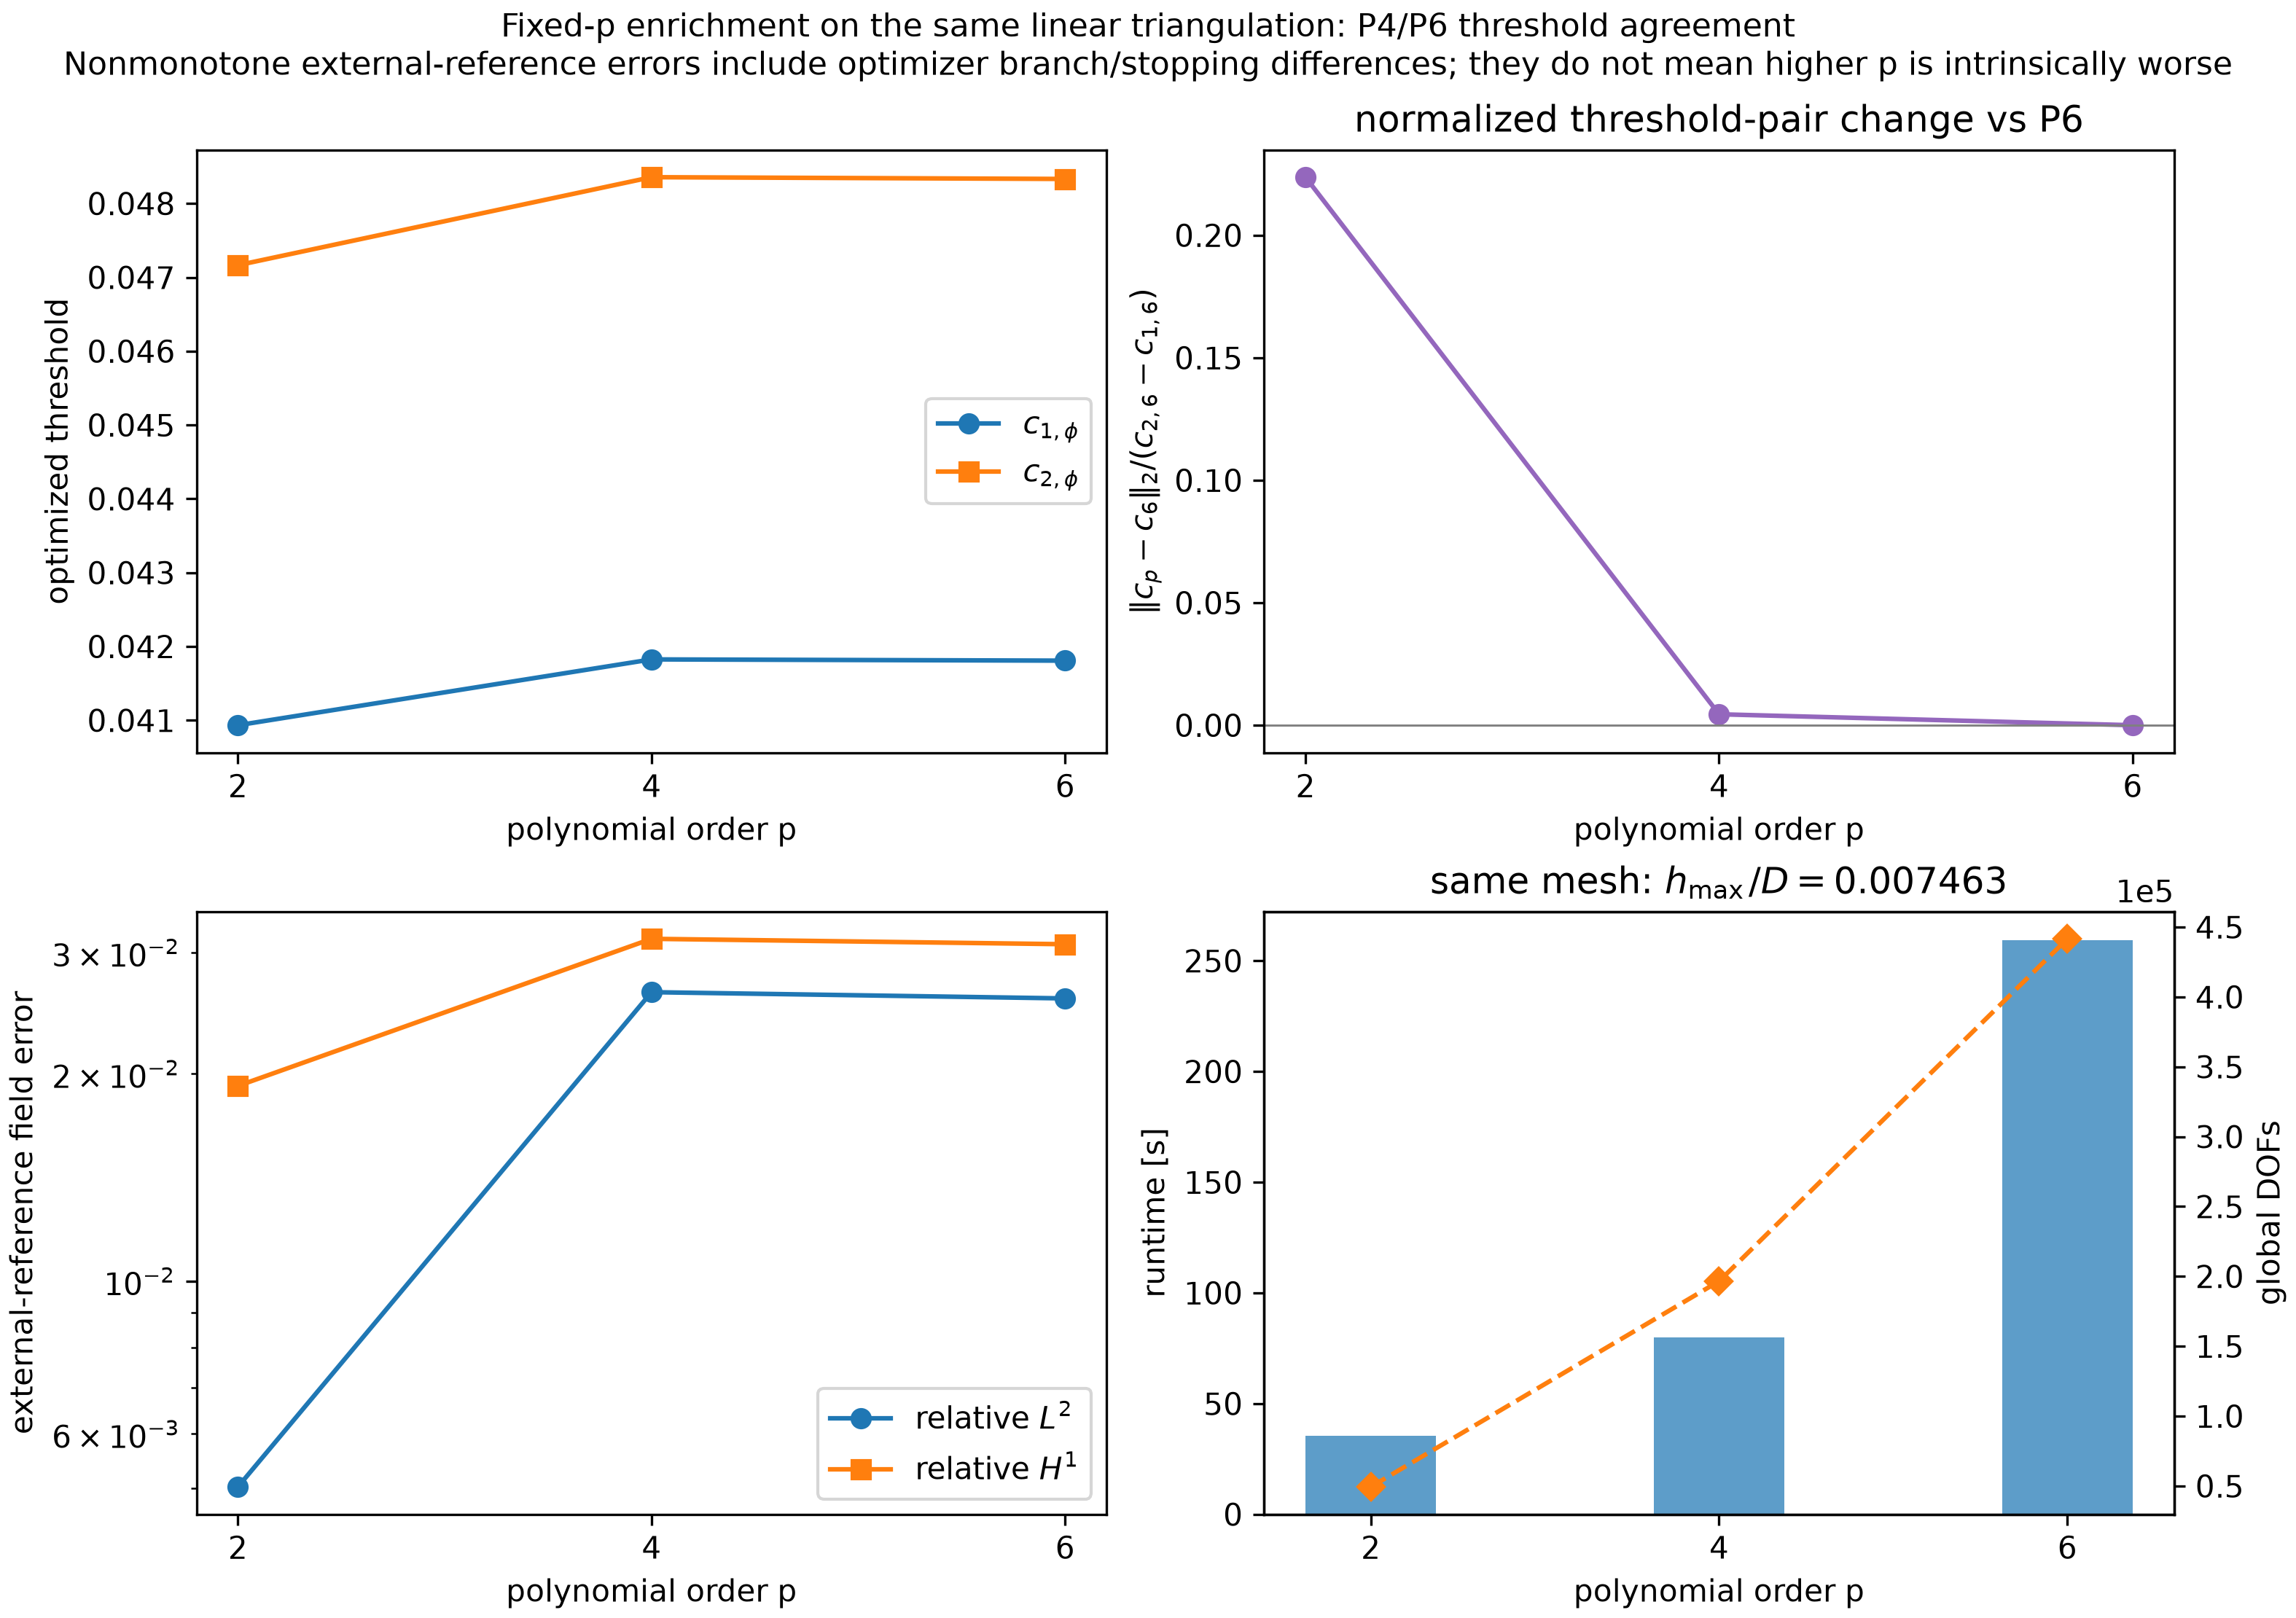
\includegraphics[width=0.88\linewidth]{figures/fixed_p_enrichment.png}
\caption{Fixed-p enrichment on the same linear triangulation: P4/P6 threshold agreement is shown explicitly. Nonmonotone external-reference errors include optimizer branch/stopping differences and do not mean higher p is intrinsically worse. Data status: actual.}
\label{fig:fixed-p-enrichment}
\end{figure}

\begin{figure}[tbp]
\centering
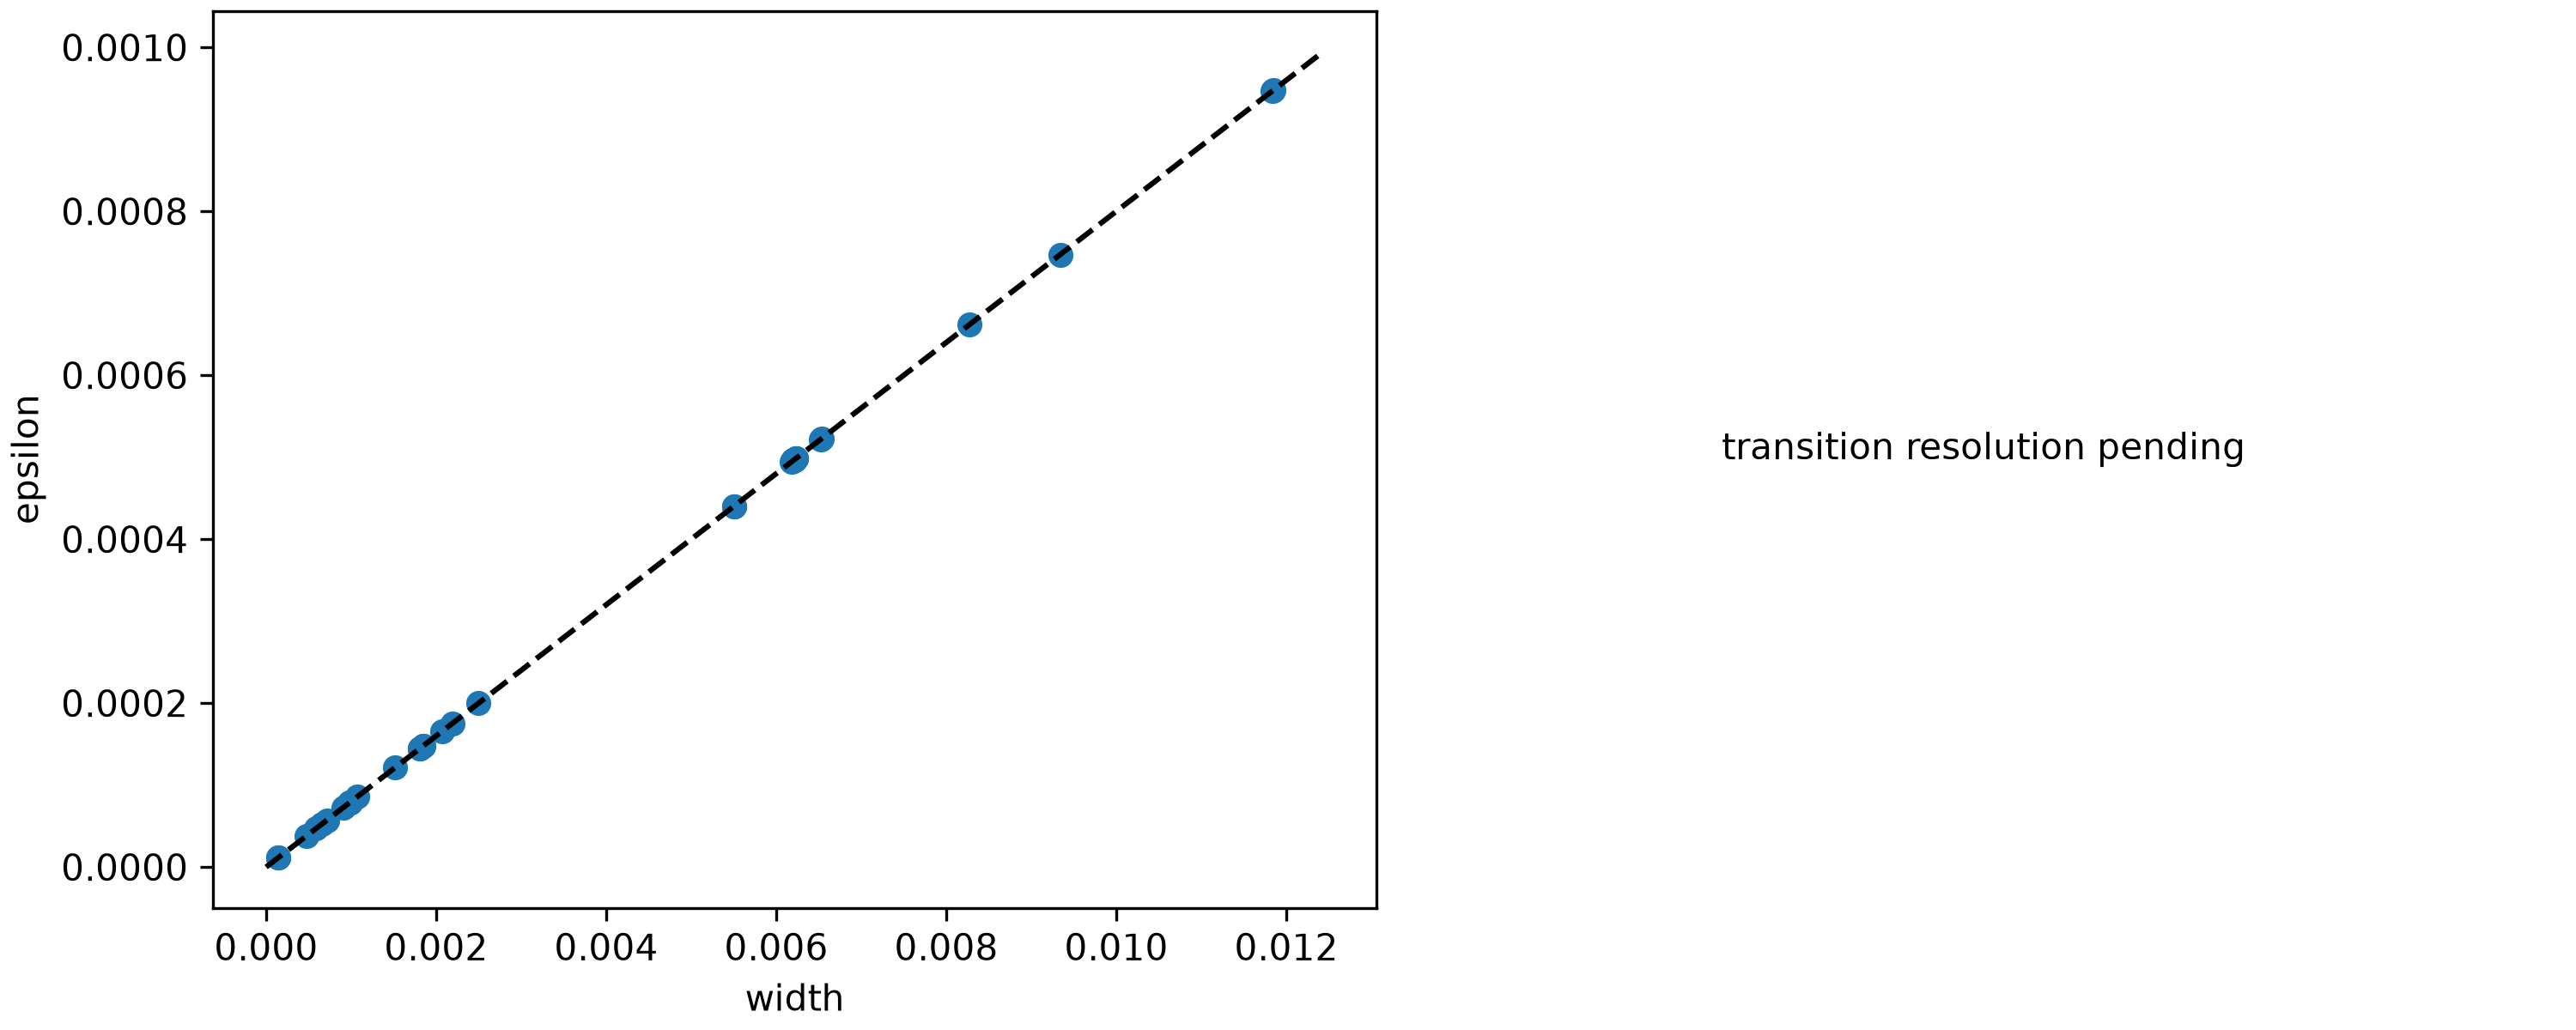
\includegraphics[width=0.88\linewidth]{figures/epsilon_transition_resolution.png}
\caption{Epsilon--width coupling and transition resolution. Data status: partial.}
\label{fig:epsilon-transition}
\end{figure}

\begin{figure}[tbp]
\centering
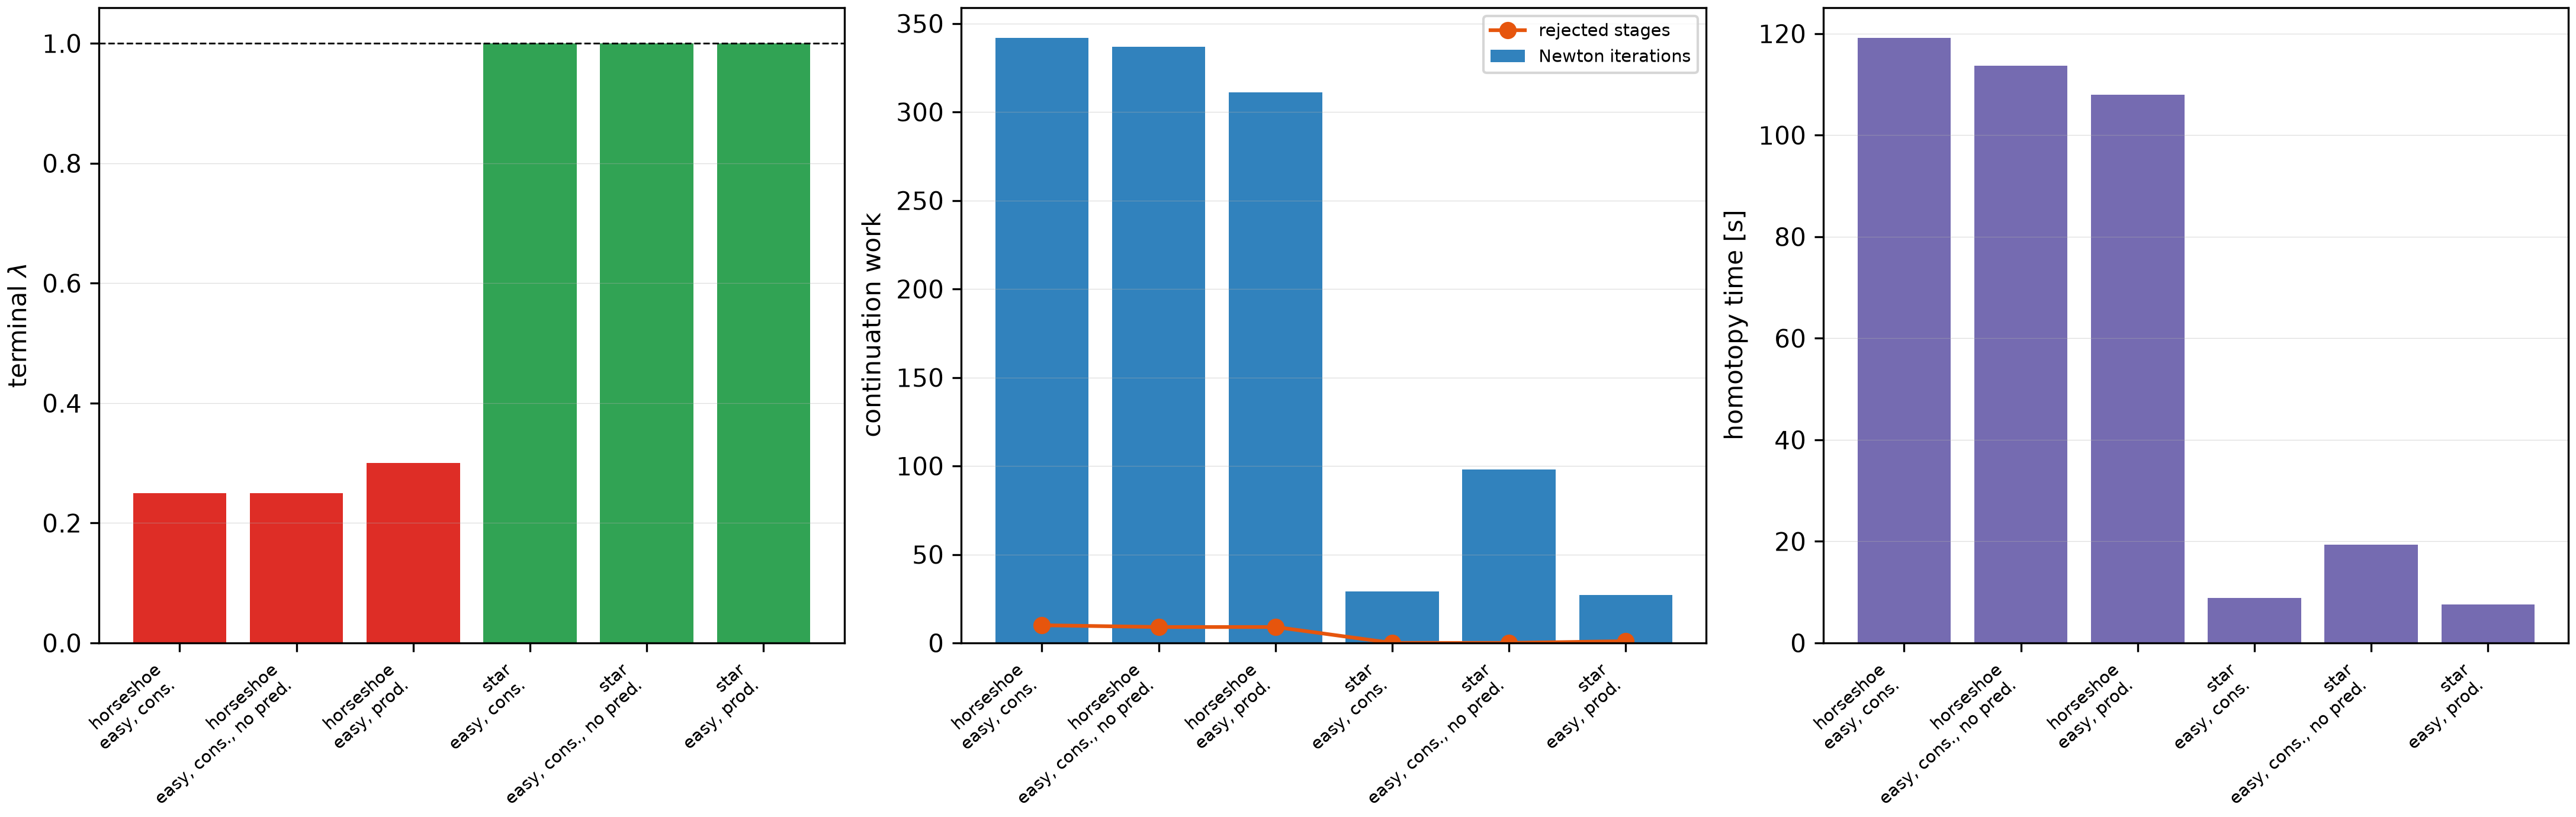
\includegraphics[width=0.88\linewidth]{figures/homotopy_robustness.png}
\caption{Continuation success, work, and runtime. Data status: partial.}
\label{fig:homotopy-robustness}
\end{figure}

\begin{figure}[tbp]
\centering
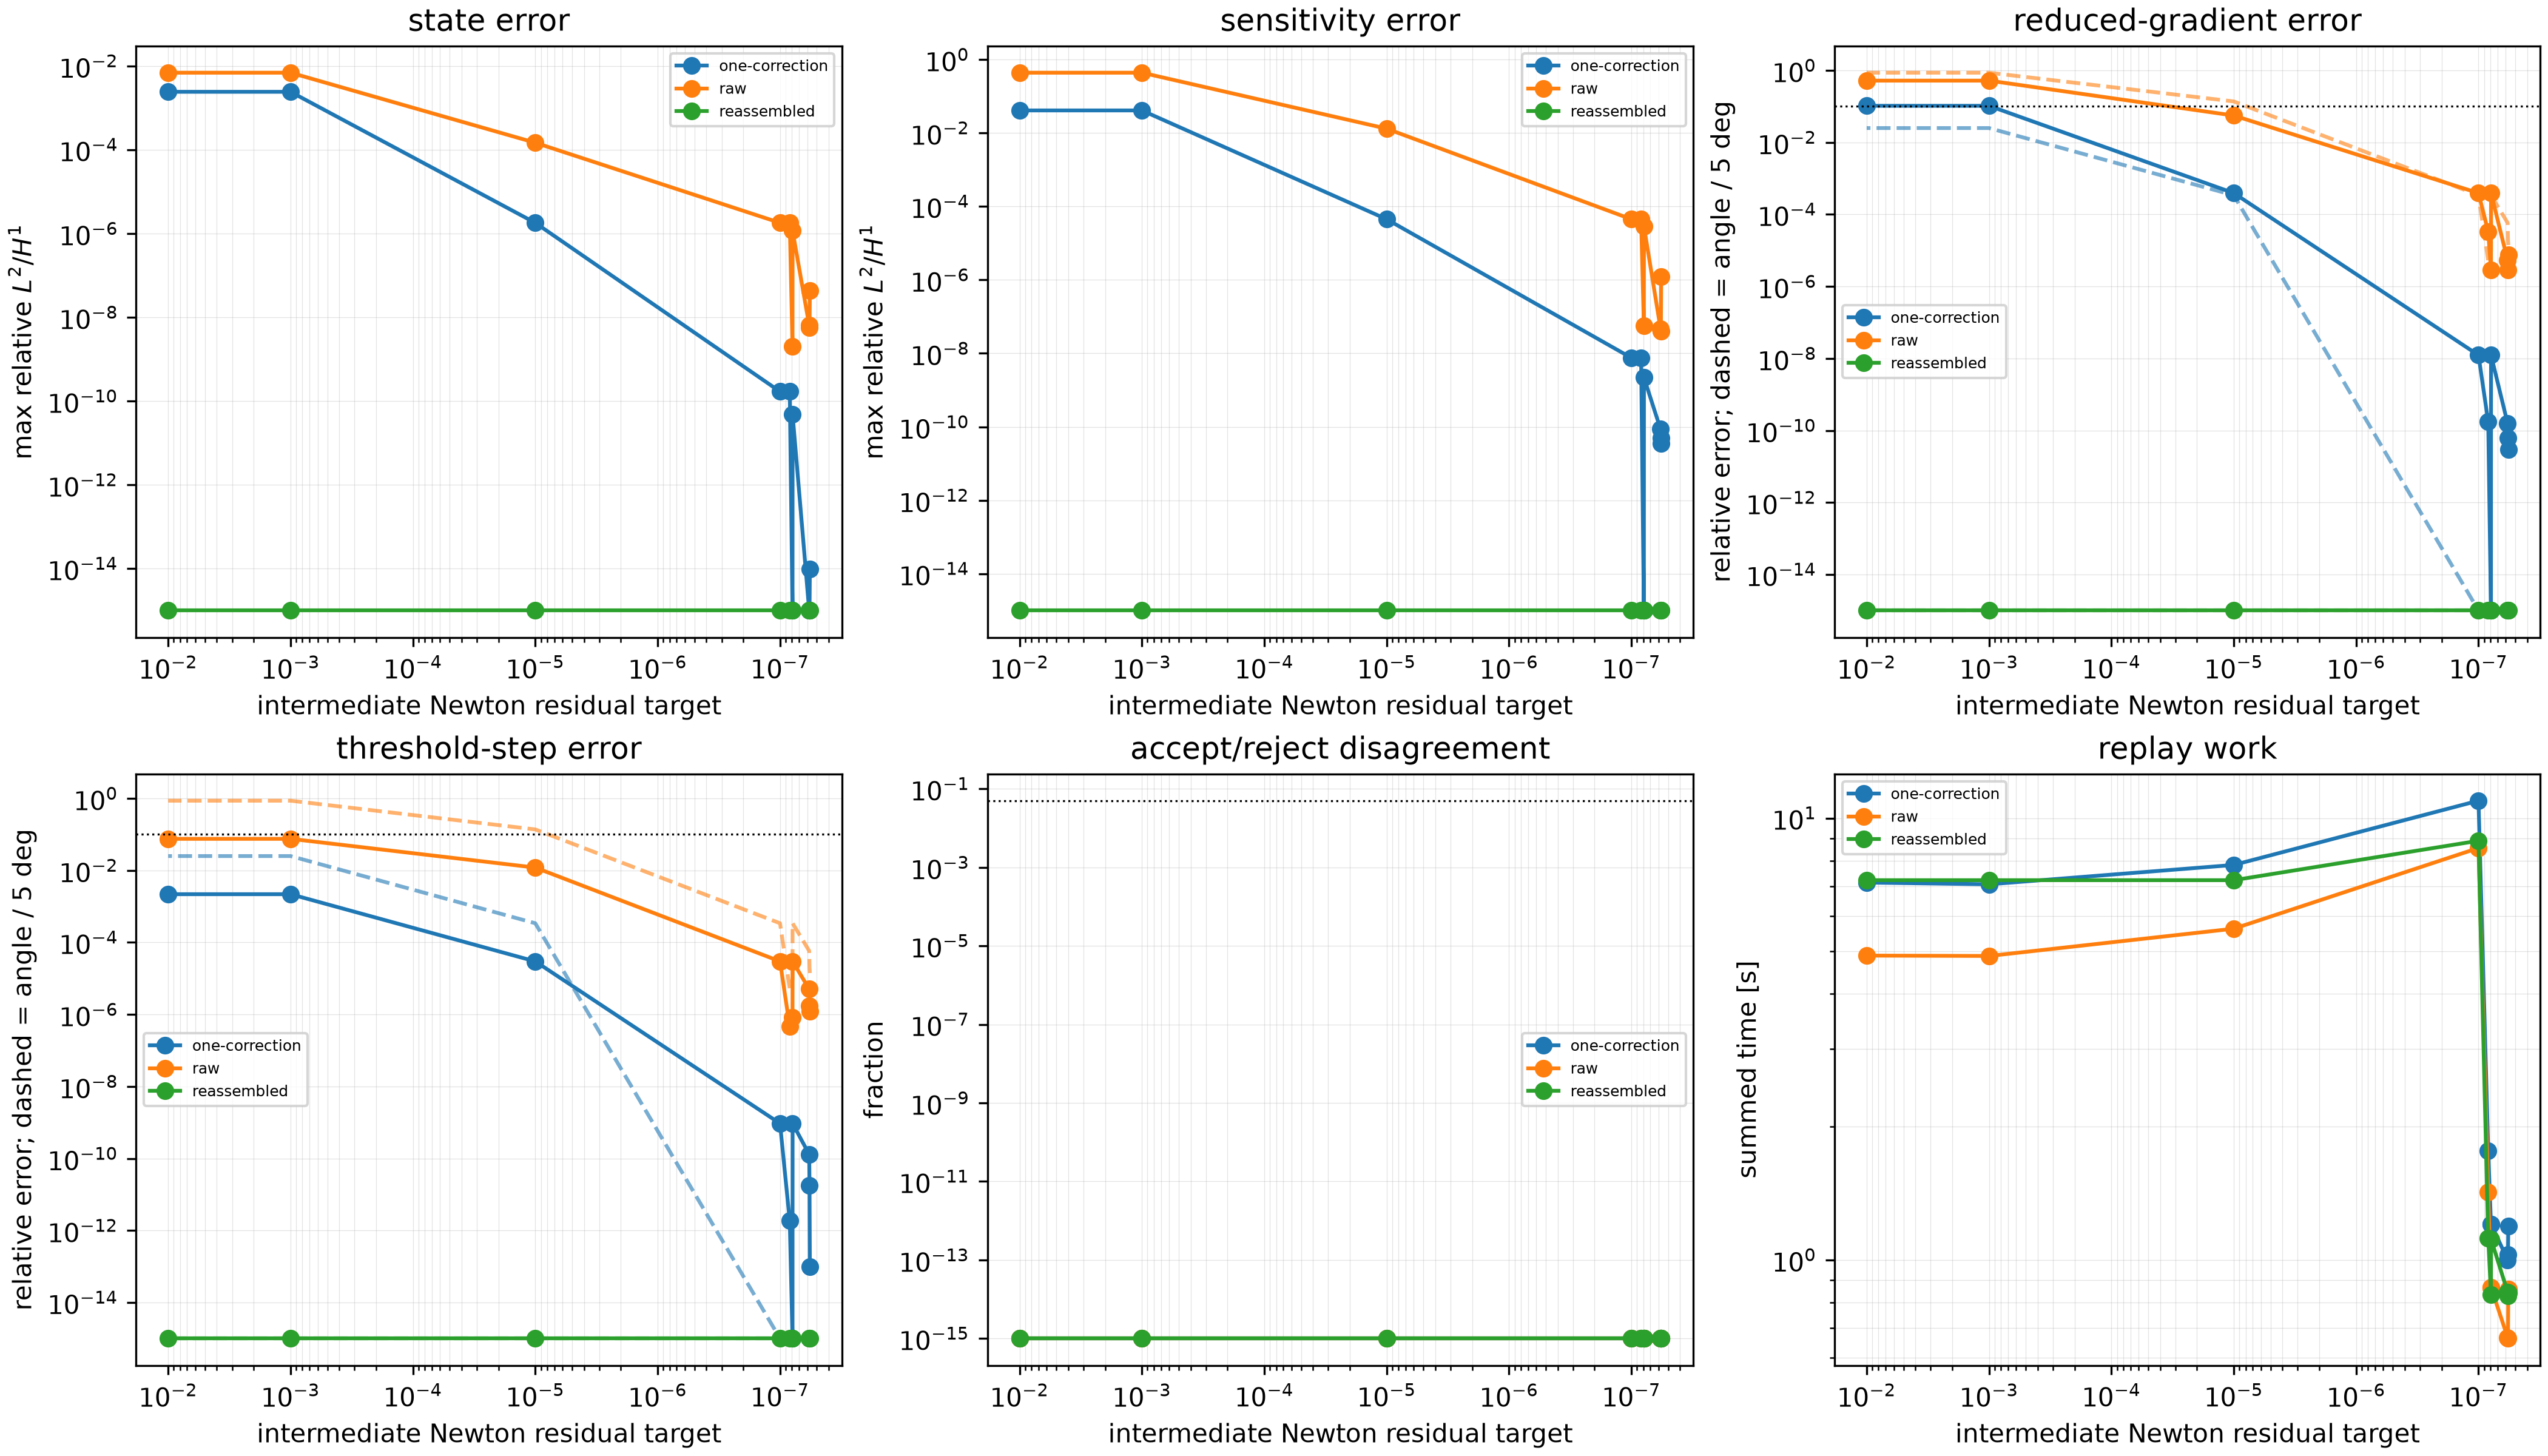
\includegraphics[width=0.88\linewidth]{figures/inner_newton_accuracy.png}
\caption{Inexact intermediate-state errors relative to tight MUMPS references: state and sensitivity fields, reduced gradient, threshold step, acceptance decisions, and work. Data status: actual.}
\label{fig:inner-newton}
\end{figure}

\begin{figure}[tbp]
\centering
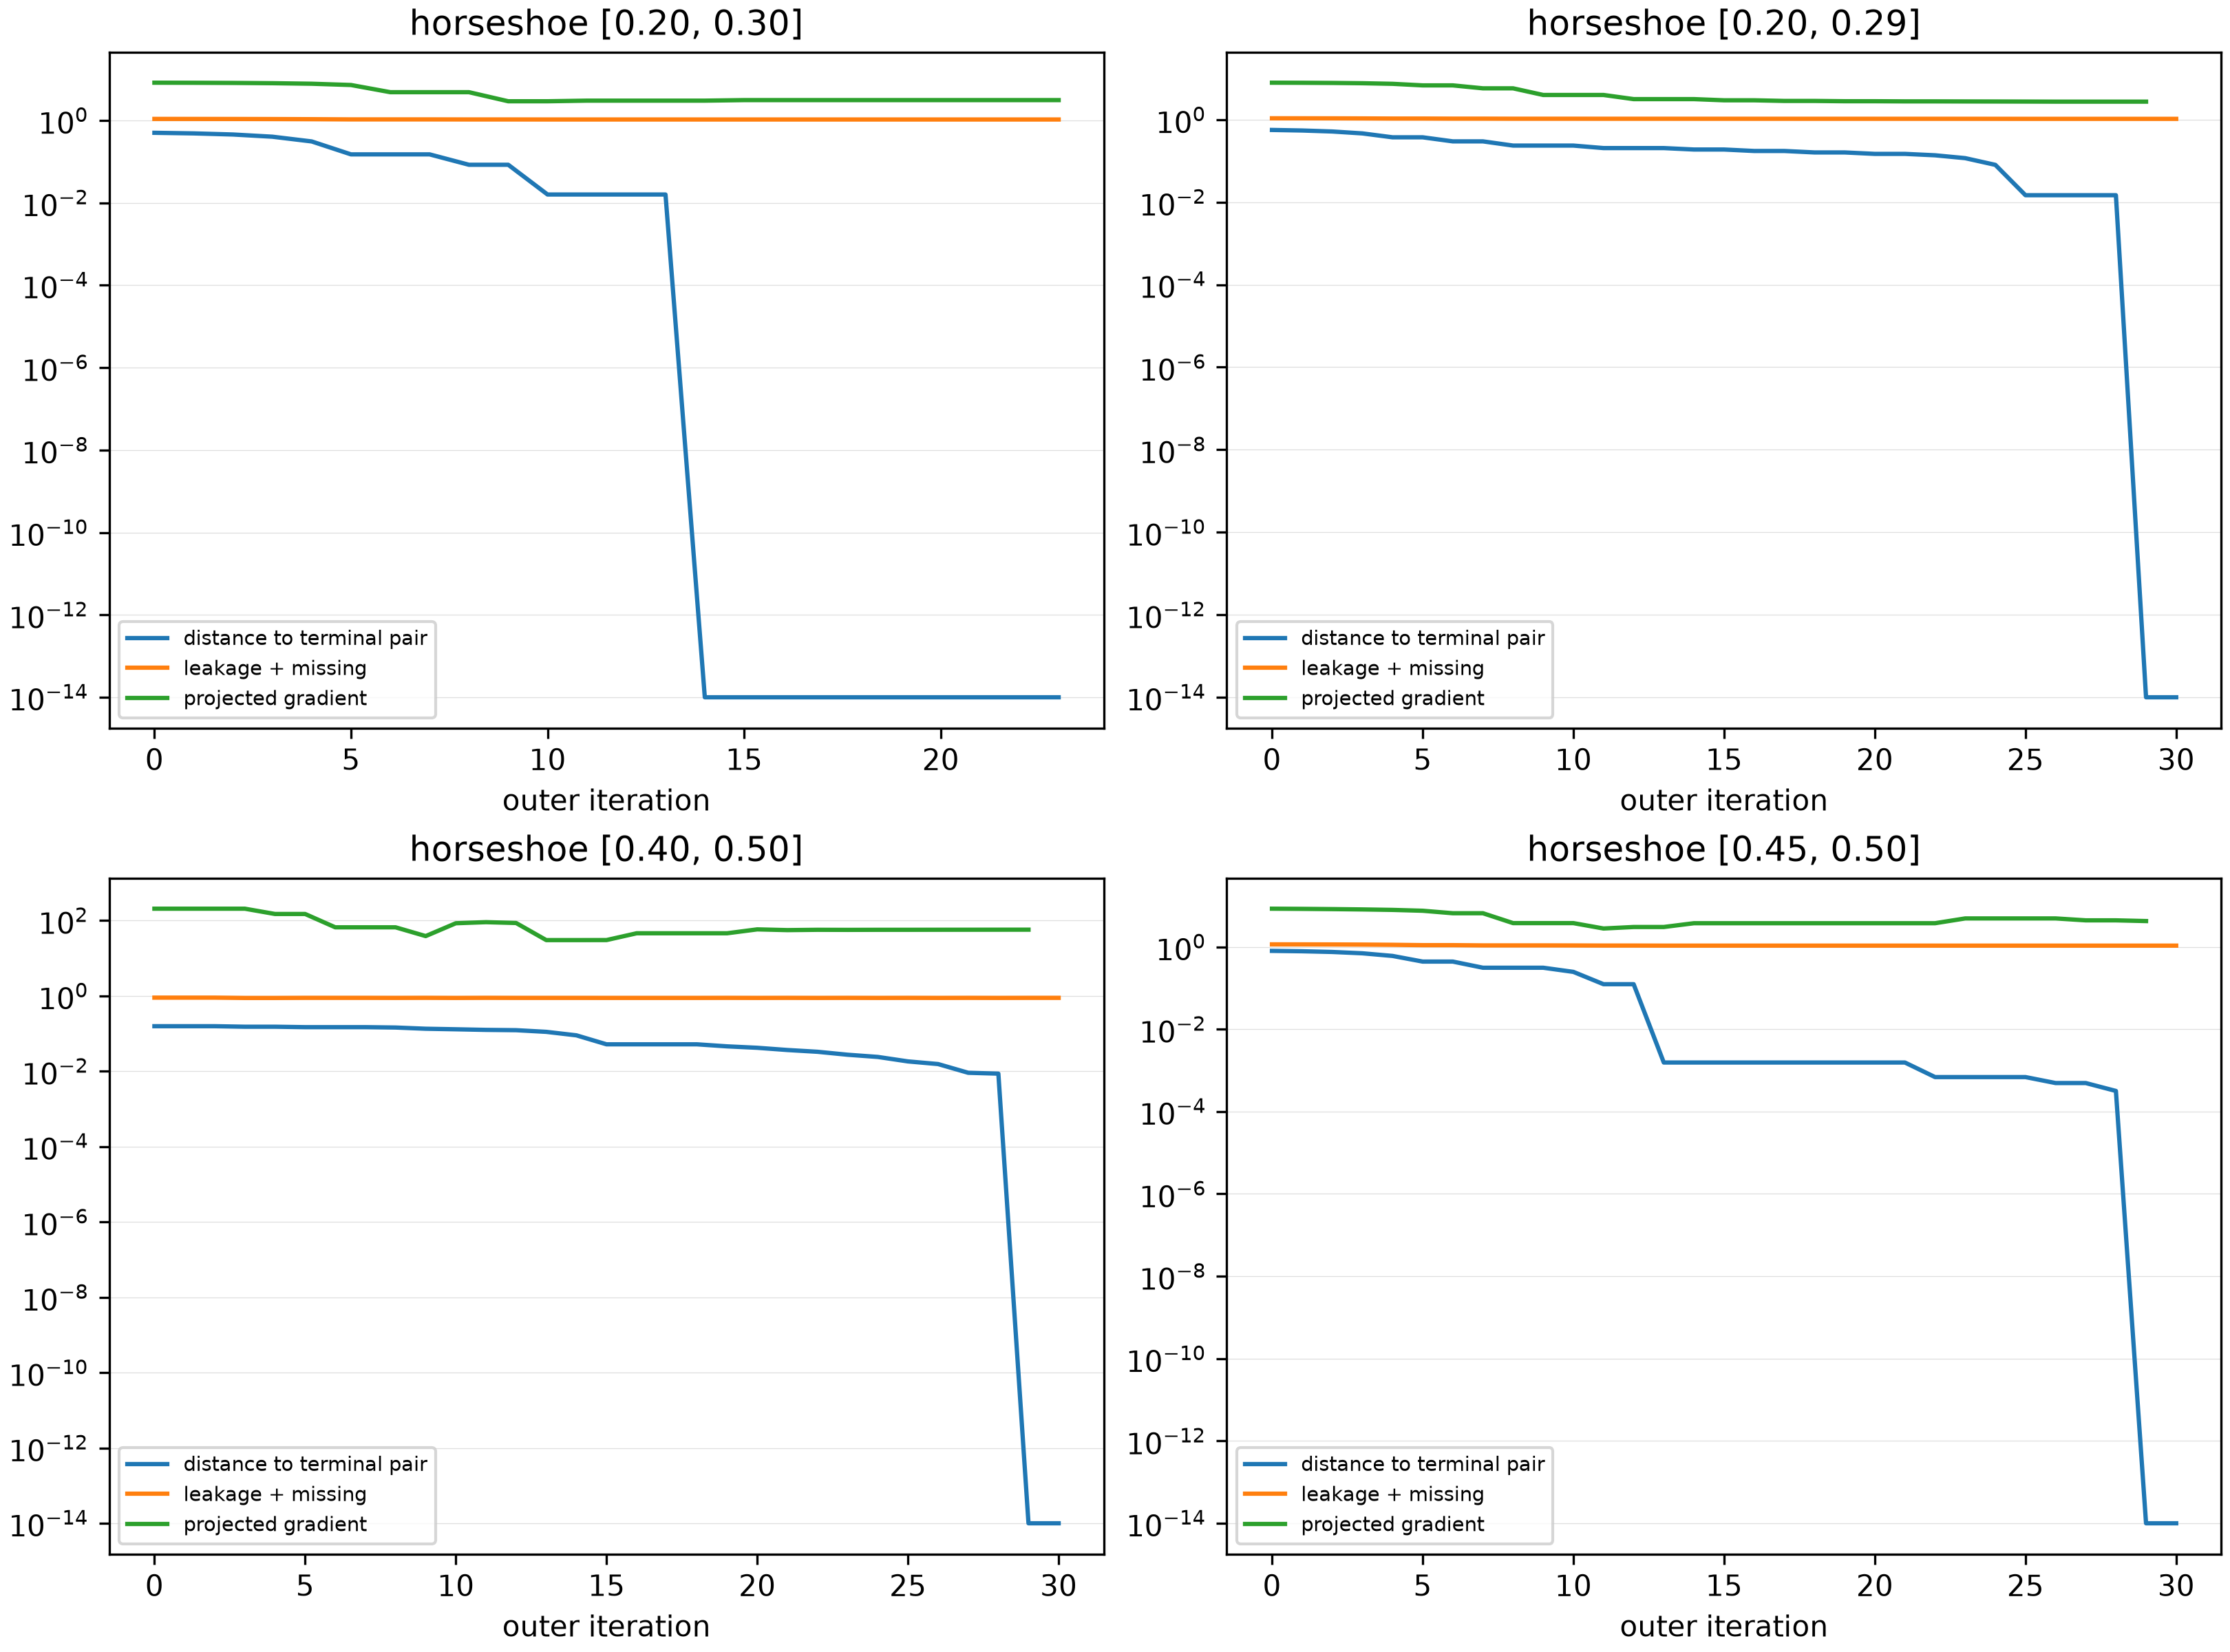
\includegraphics[width=0.88\linewidth]{figures/threshold_optimization_plateaus.png}
\caption{Threshold-space plateau diagnostics. Data status: actual.}
\label{fig:threshold-plateau}
\end{figure}

\begin{figure}[tbp]
\centering
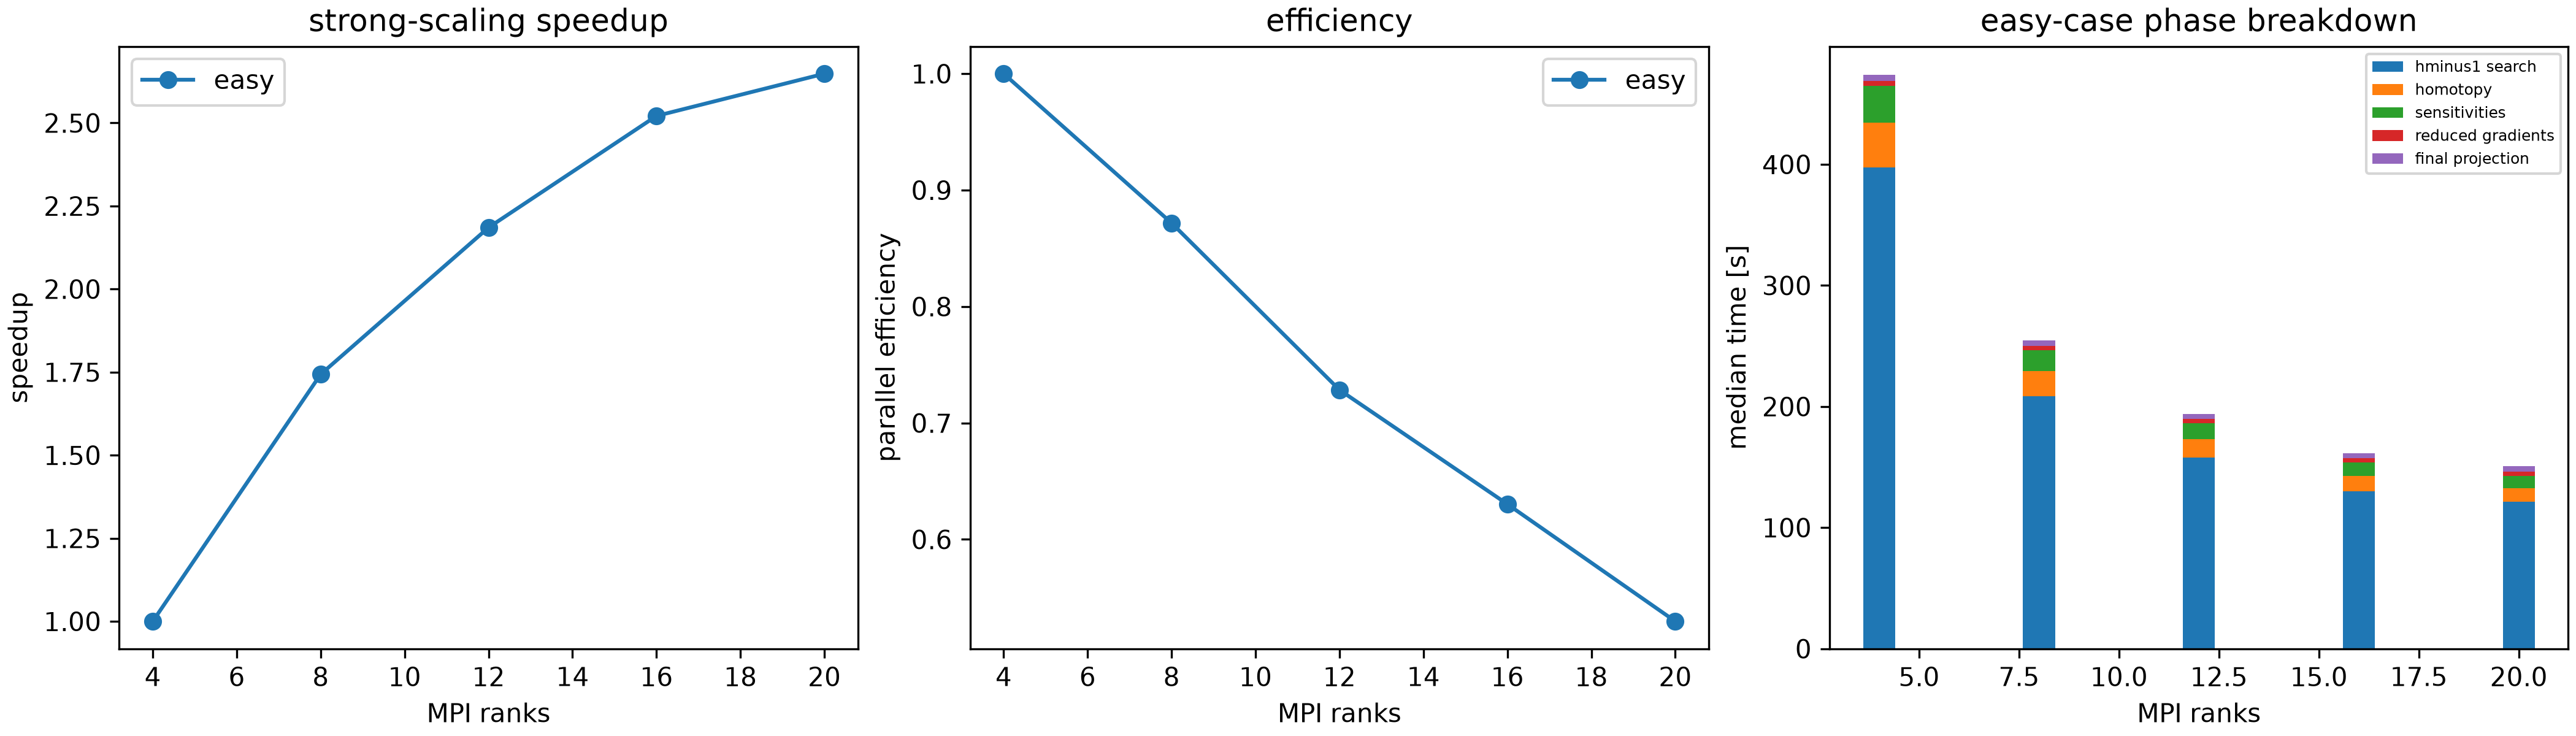
\includegraphics[width=0.88\linewidth]{figures/strong_scaling_summary.png}
\caption{Strong scaling, efficiency, and phase breakdown. Data status: actual.}
\label{fig:strong-scaling}
\end{figure}

\begin{figure}[tbp]
\centering
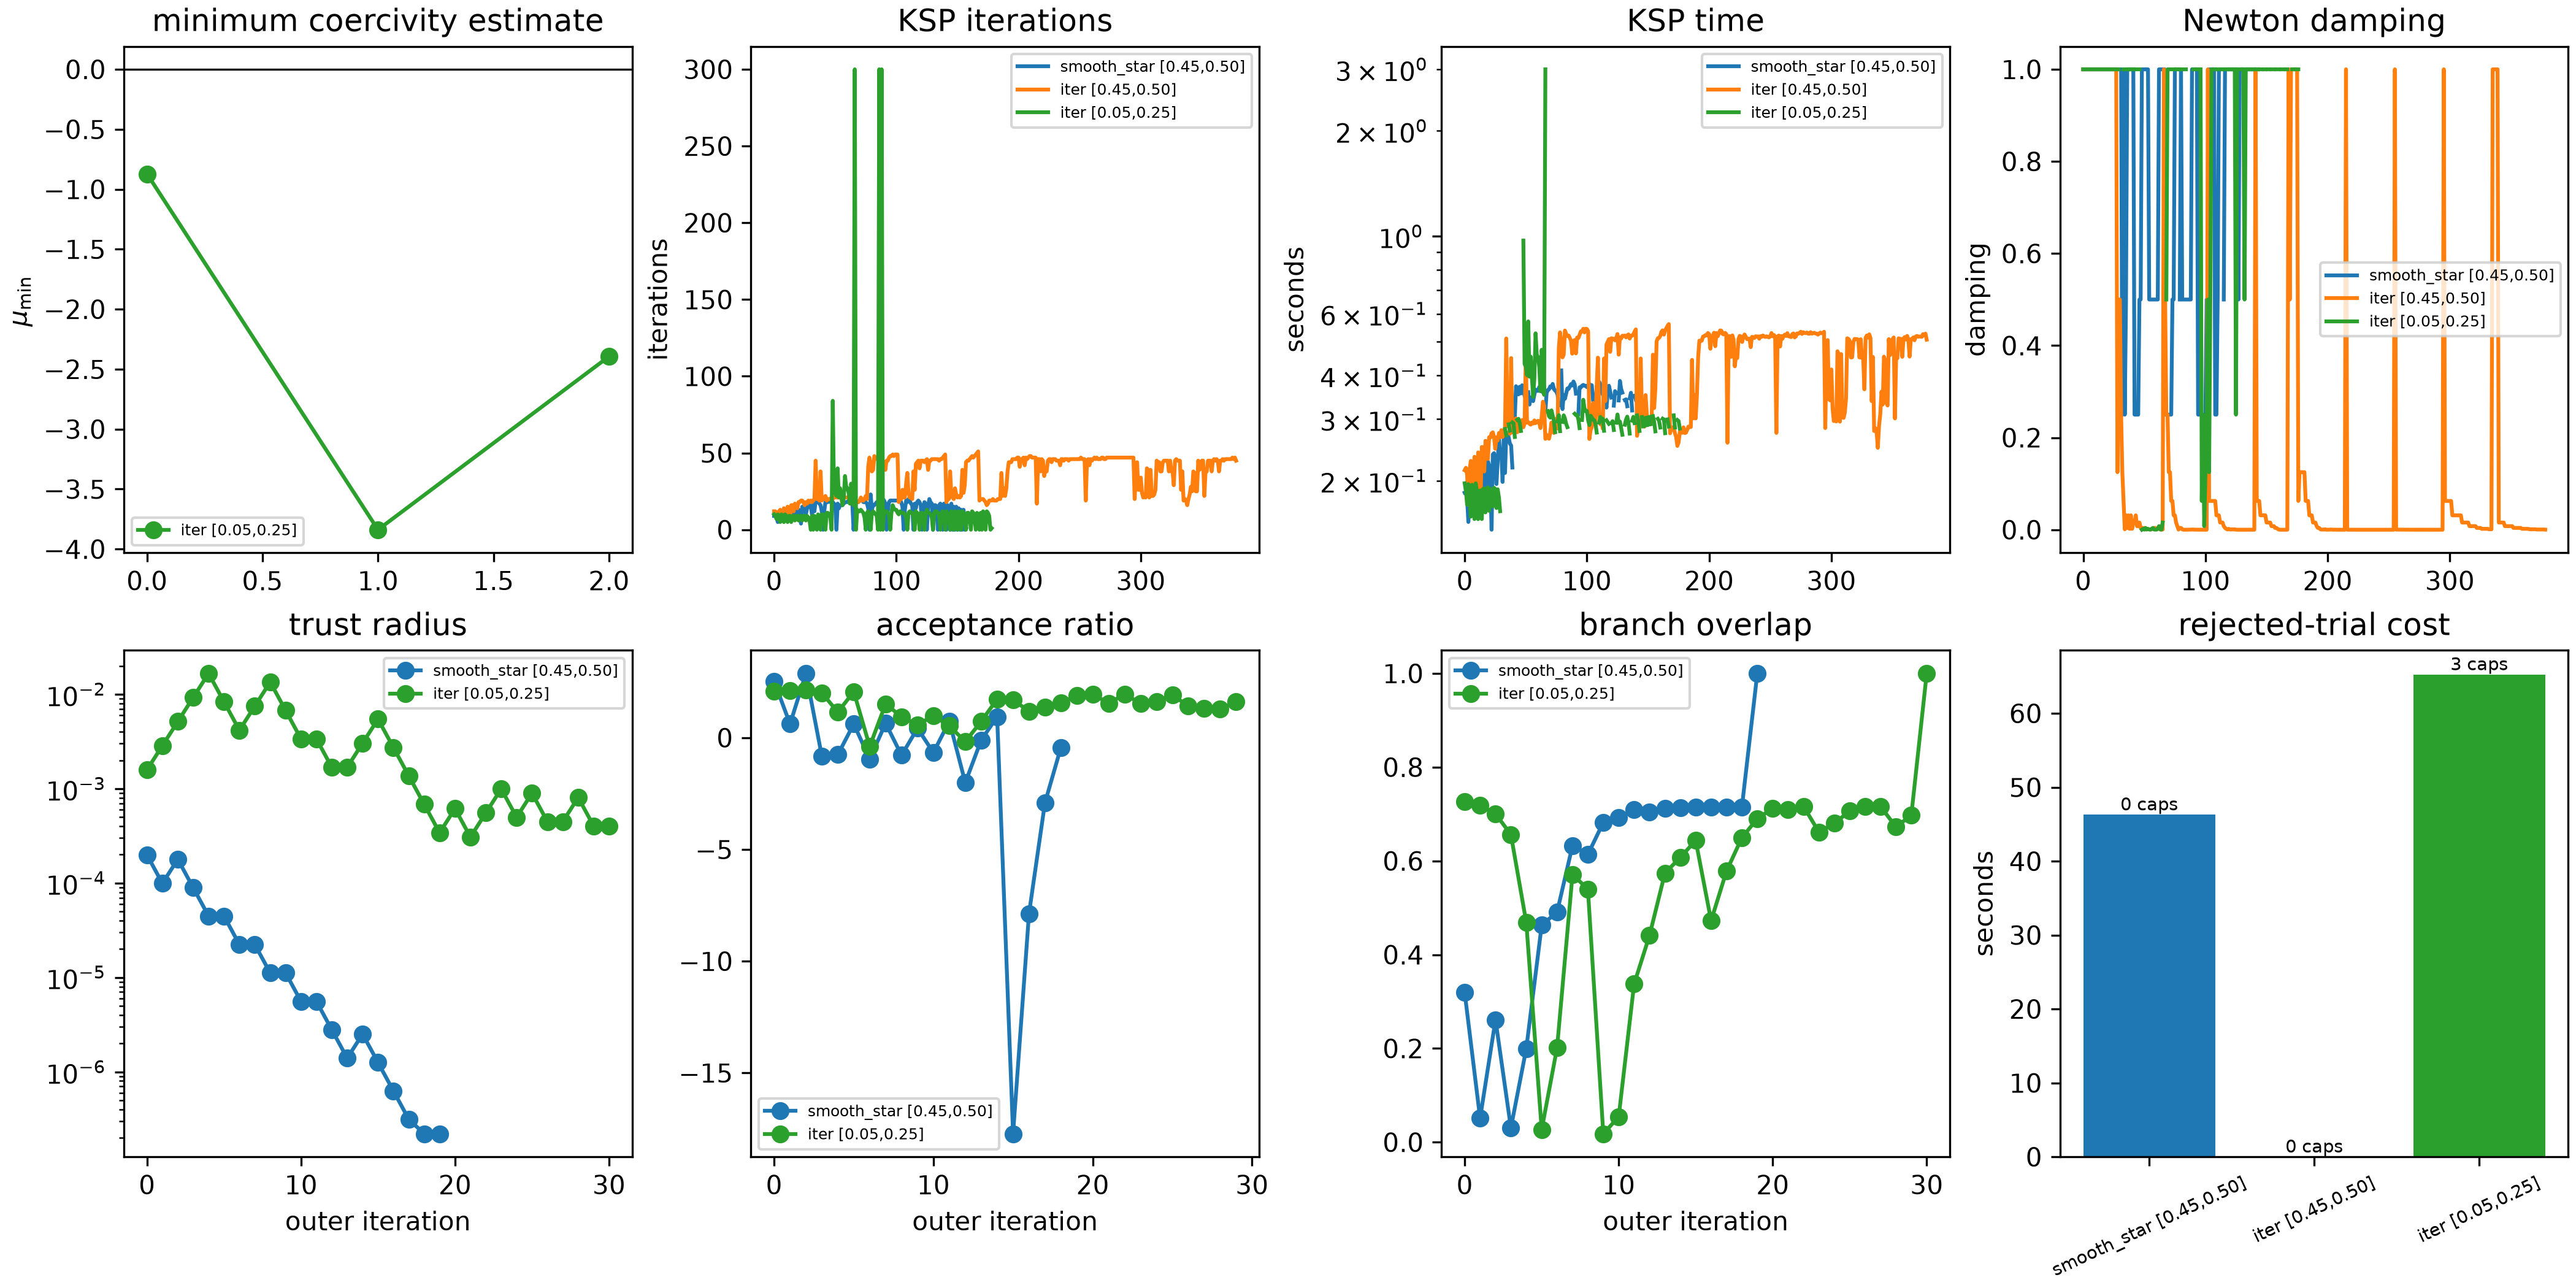
\includegraphics[width=0.88\linewidth]{figures/coercivity_diagnostics.png}
\caption{Capped-trial coercivity and rejected-trial cost. Data status: actual.}
\label{fig:coercivity}
\end{figure}

\clearpage

\begin{landscape}
\begin{figure}[tbp]
\centering
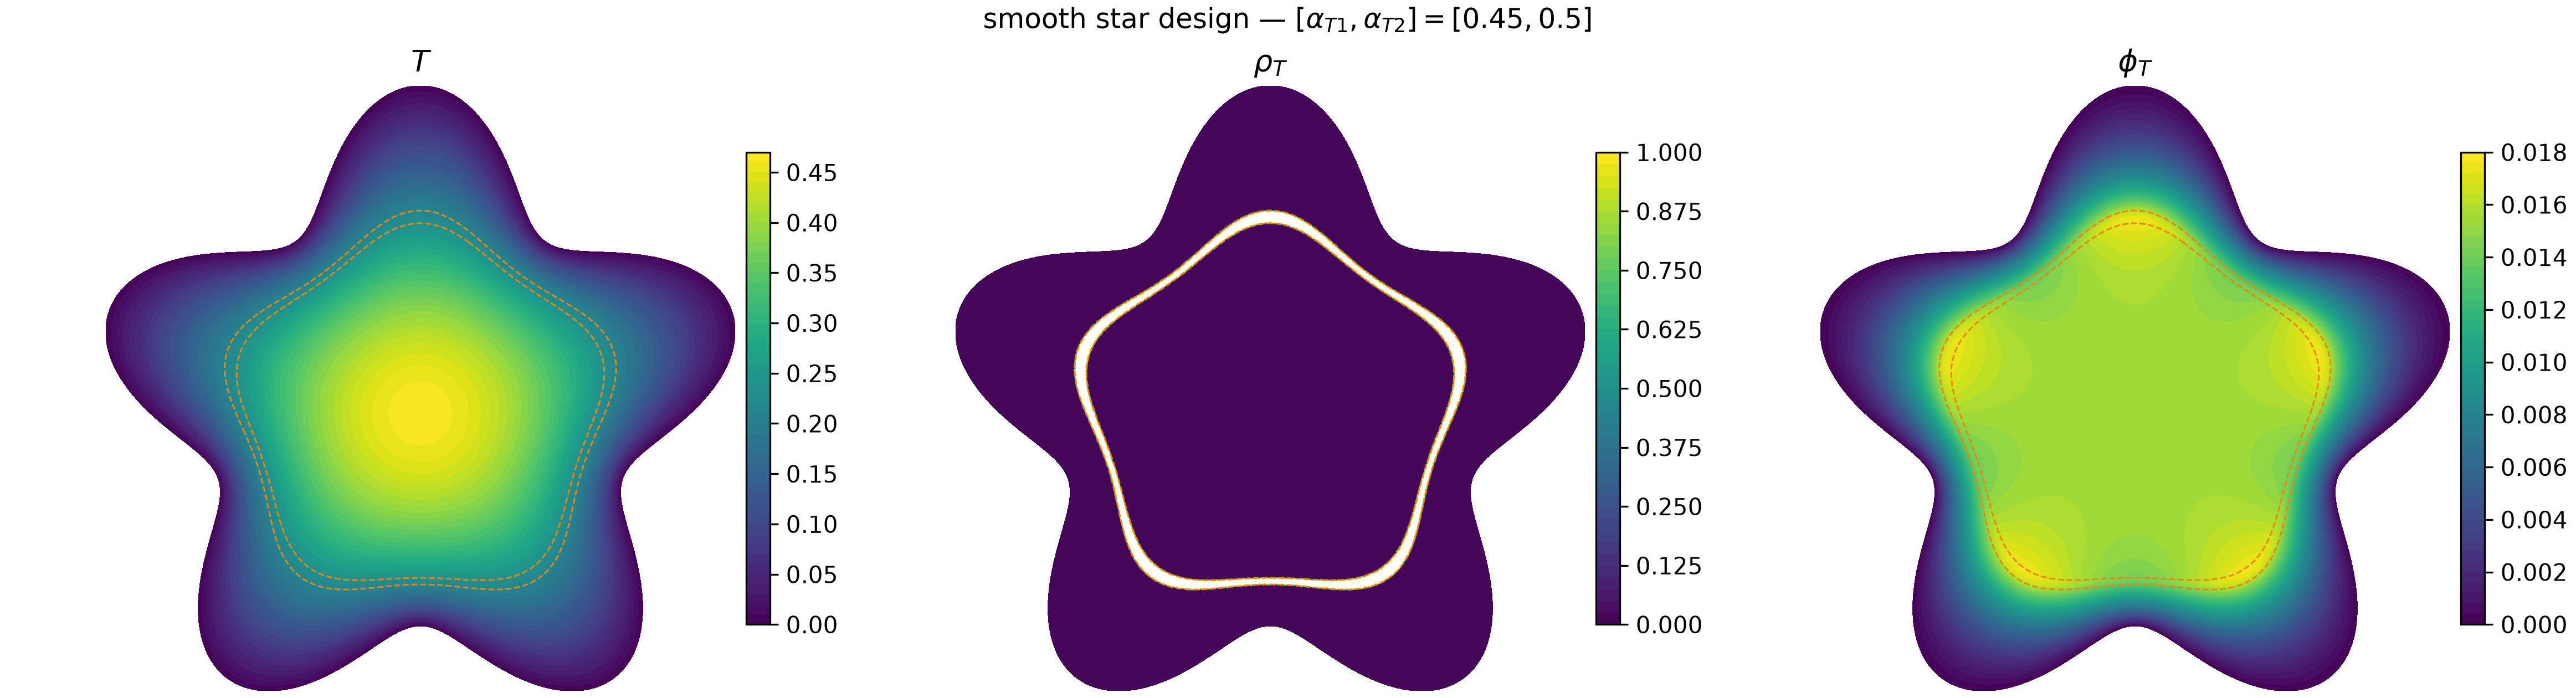
\includegraphics[width=0.97\linewidth]{figures/design_fields_smooth_star_0p45_0p5.png}
\caption{Smooth Star design fields for torsion levels $[0.45,0.5]$: torsion, target density, and target potential.  The design is shown once; orange dashed curves mark its fixed band boundaries. Data status: actual.}
\label{fig:design-fields-smooth-star}
\end{figure}
\end{landscape}

\begin{landscape}
\begin{figure}[tbp]
\centering
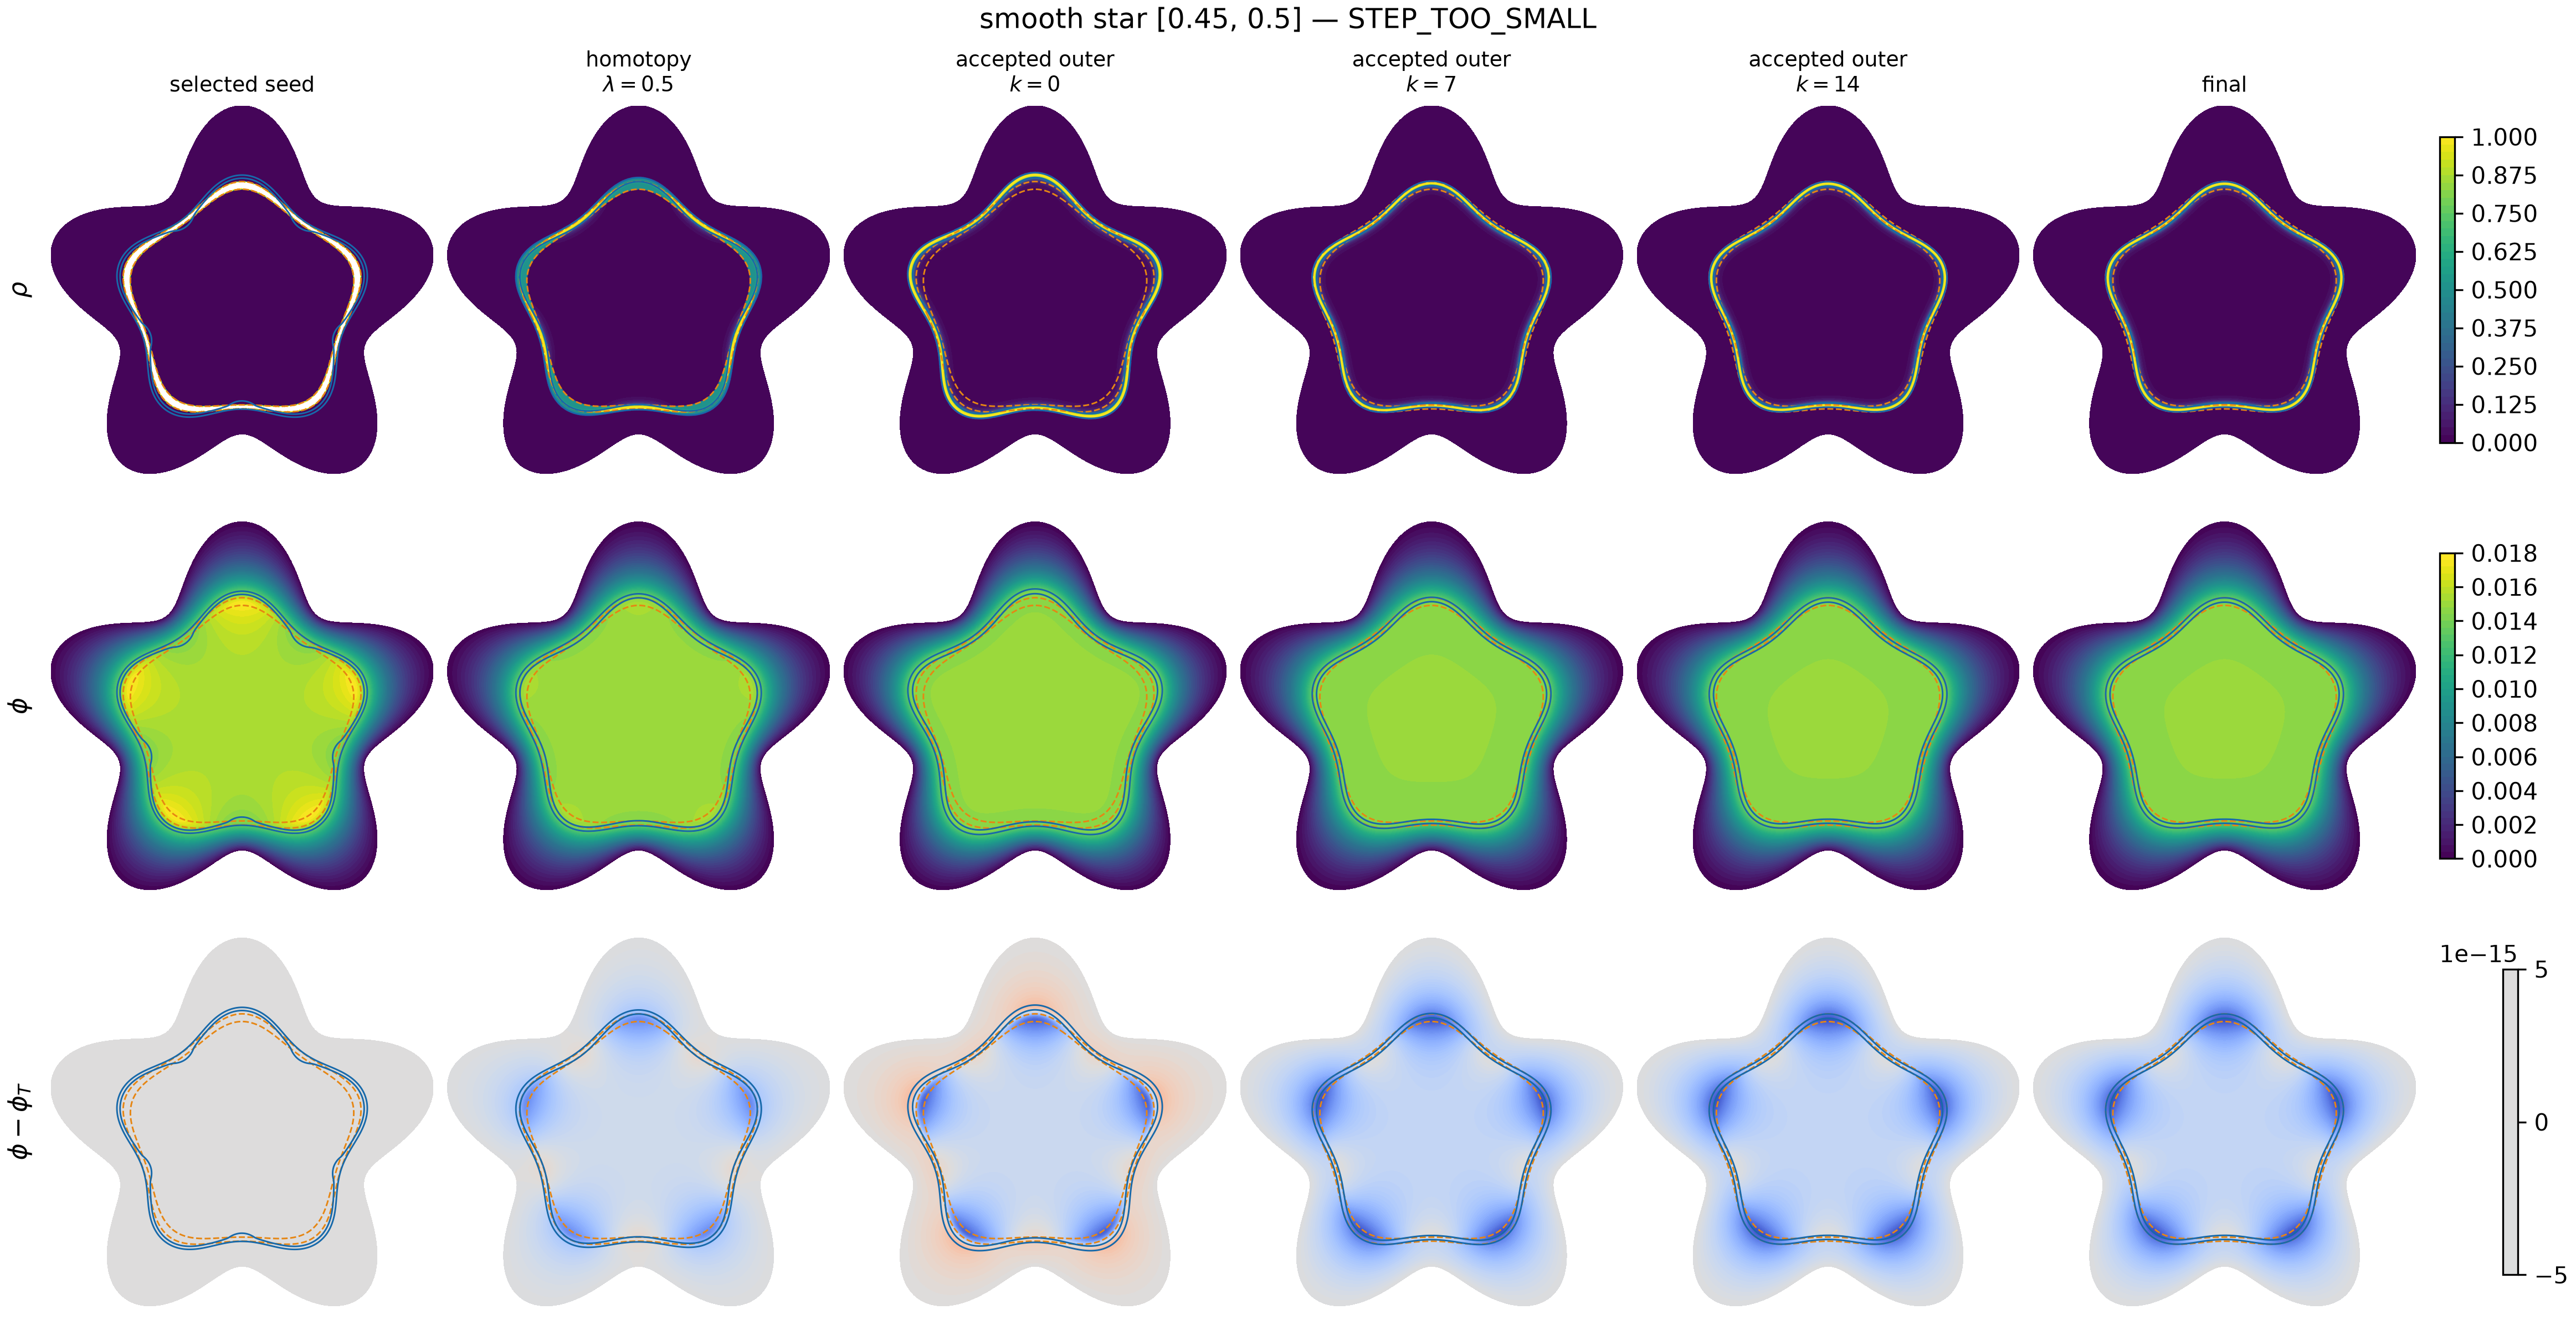
\includegraphics[width=0.97\linewidth]{figures/band_evolution_smooth_star_0p45_0p5.png}
\caption{Smooth Star equilibrium formation for torsion levels $[0.45,0.5]$: selected seed, intermediate homotopy, early and middle accepted states, late or restored-best state, and final projection; PDE-converged with a retained geometric plateau.  Orange dashed curves are the fixed target band and blue solid curves are the moving equilibrium band. Data status: actual.}
\label{fig:band-evolution}
\end{figure}
\end{landscape}

\begin{landscape}
\begin{figure}[tbp]
\centering
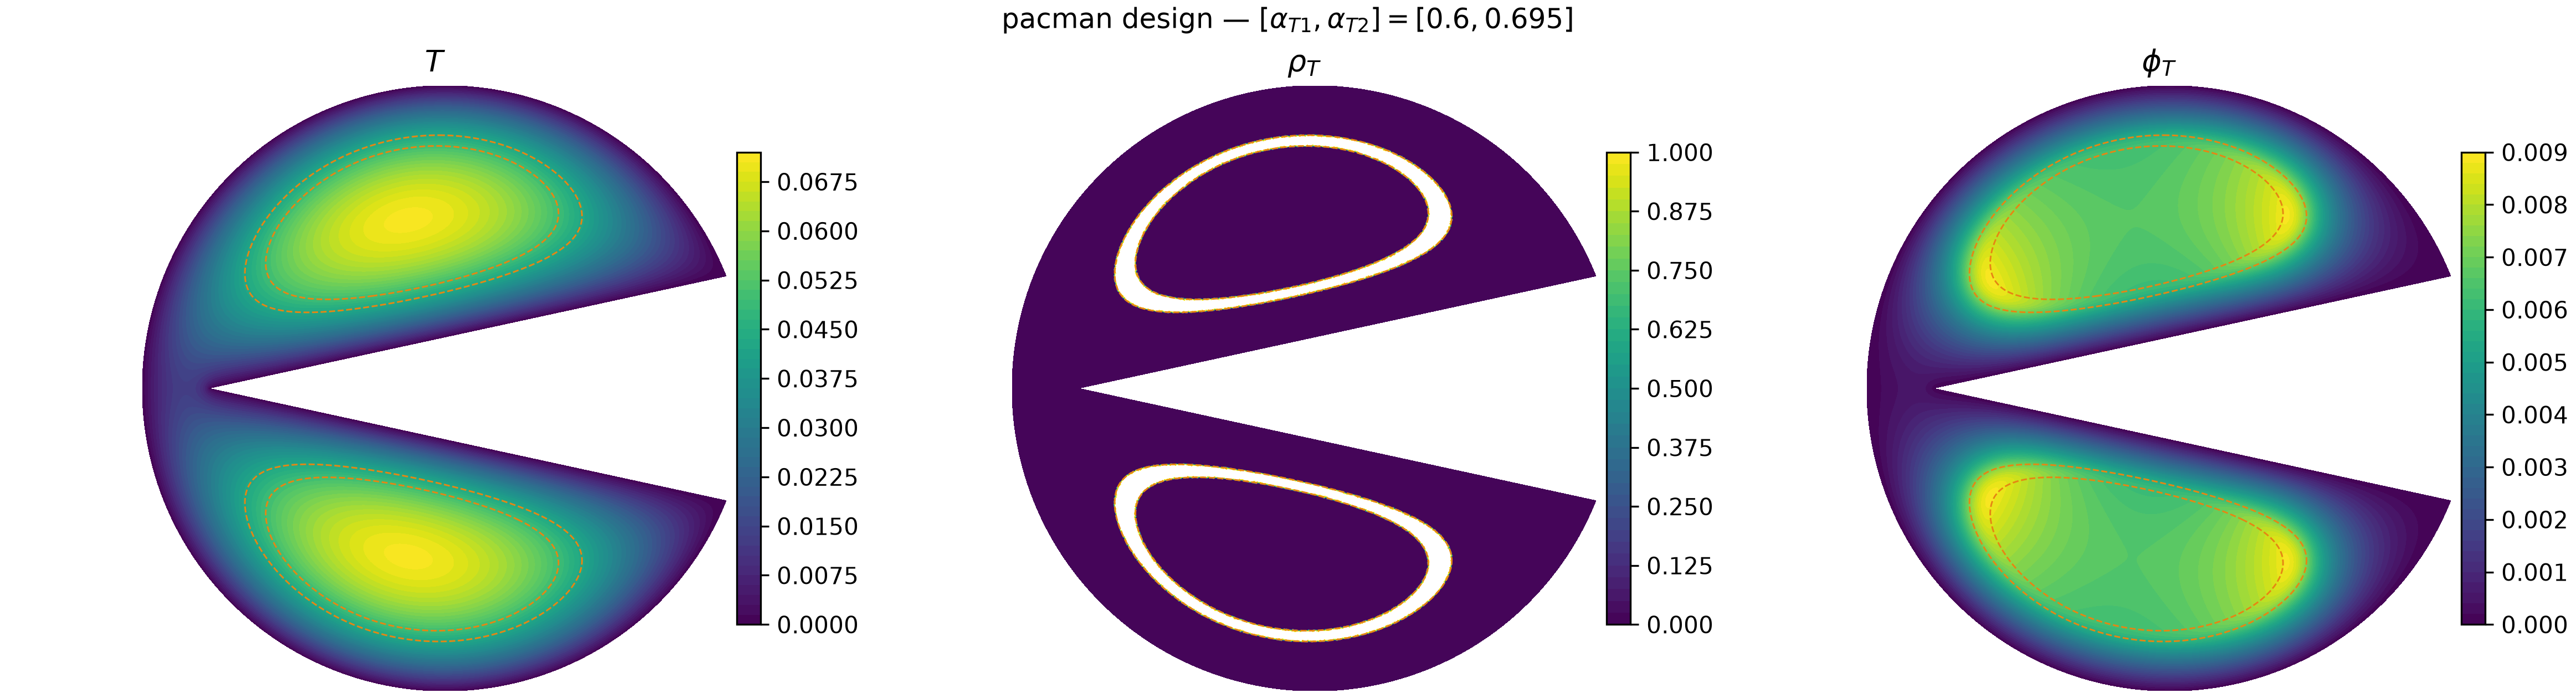
\includegraphics[width=0.97\linewidth]{figures/design_fields_pacman_0p6_0p695.png}
\caption{Pacman design fields for torsion levels $[0.6,0.695]$: torsion, target density, and target potential.  The design is shown once; orange dashed curves mark its fixed band boundaries. Data status: actual.}
\label{fig:design-fields-pacman}
\end{figure}
\end{landscape}

\begin{landscape}
\begin{figure}[tbp]
\centering
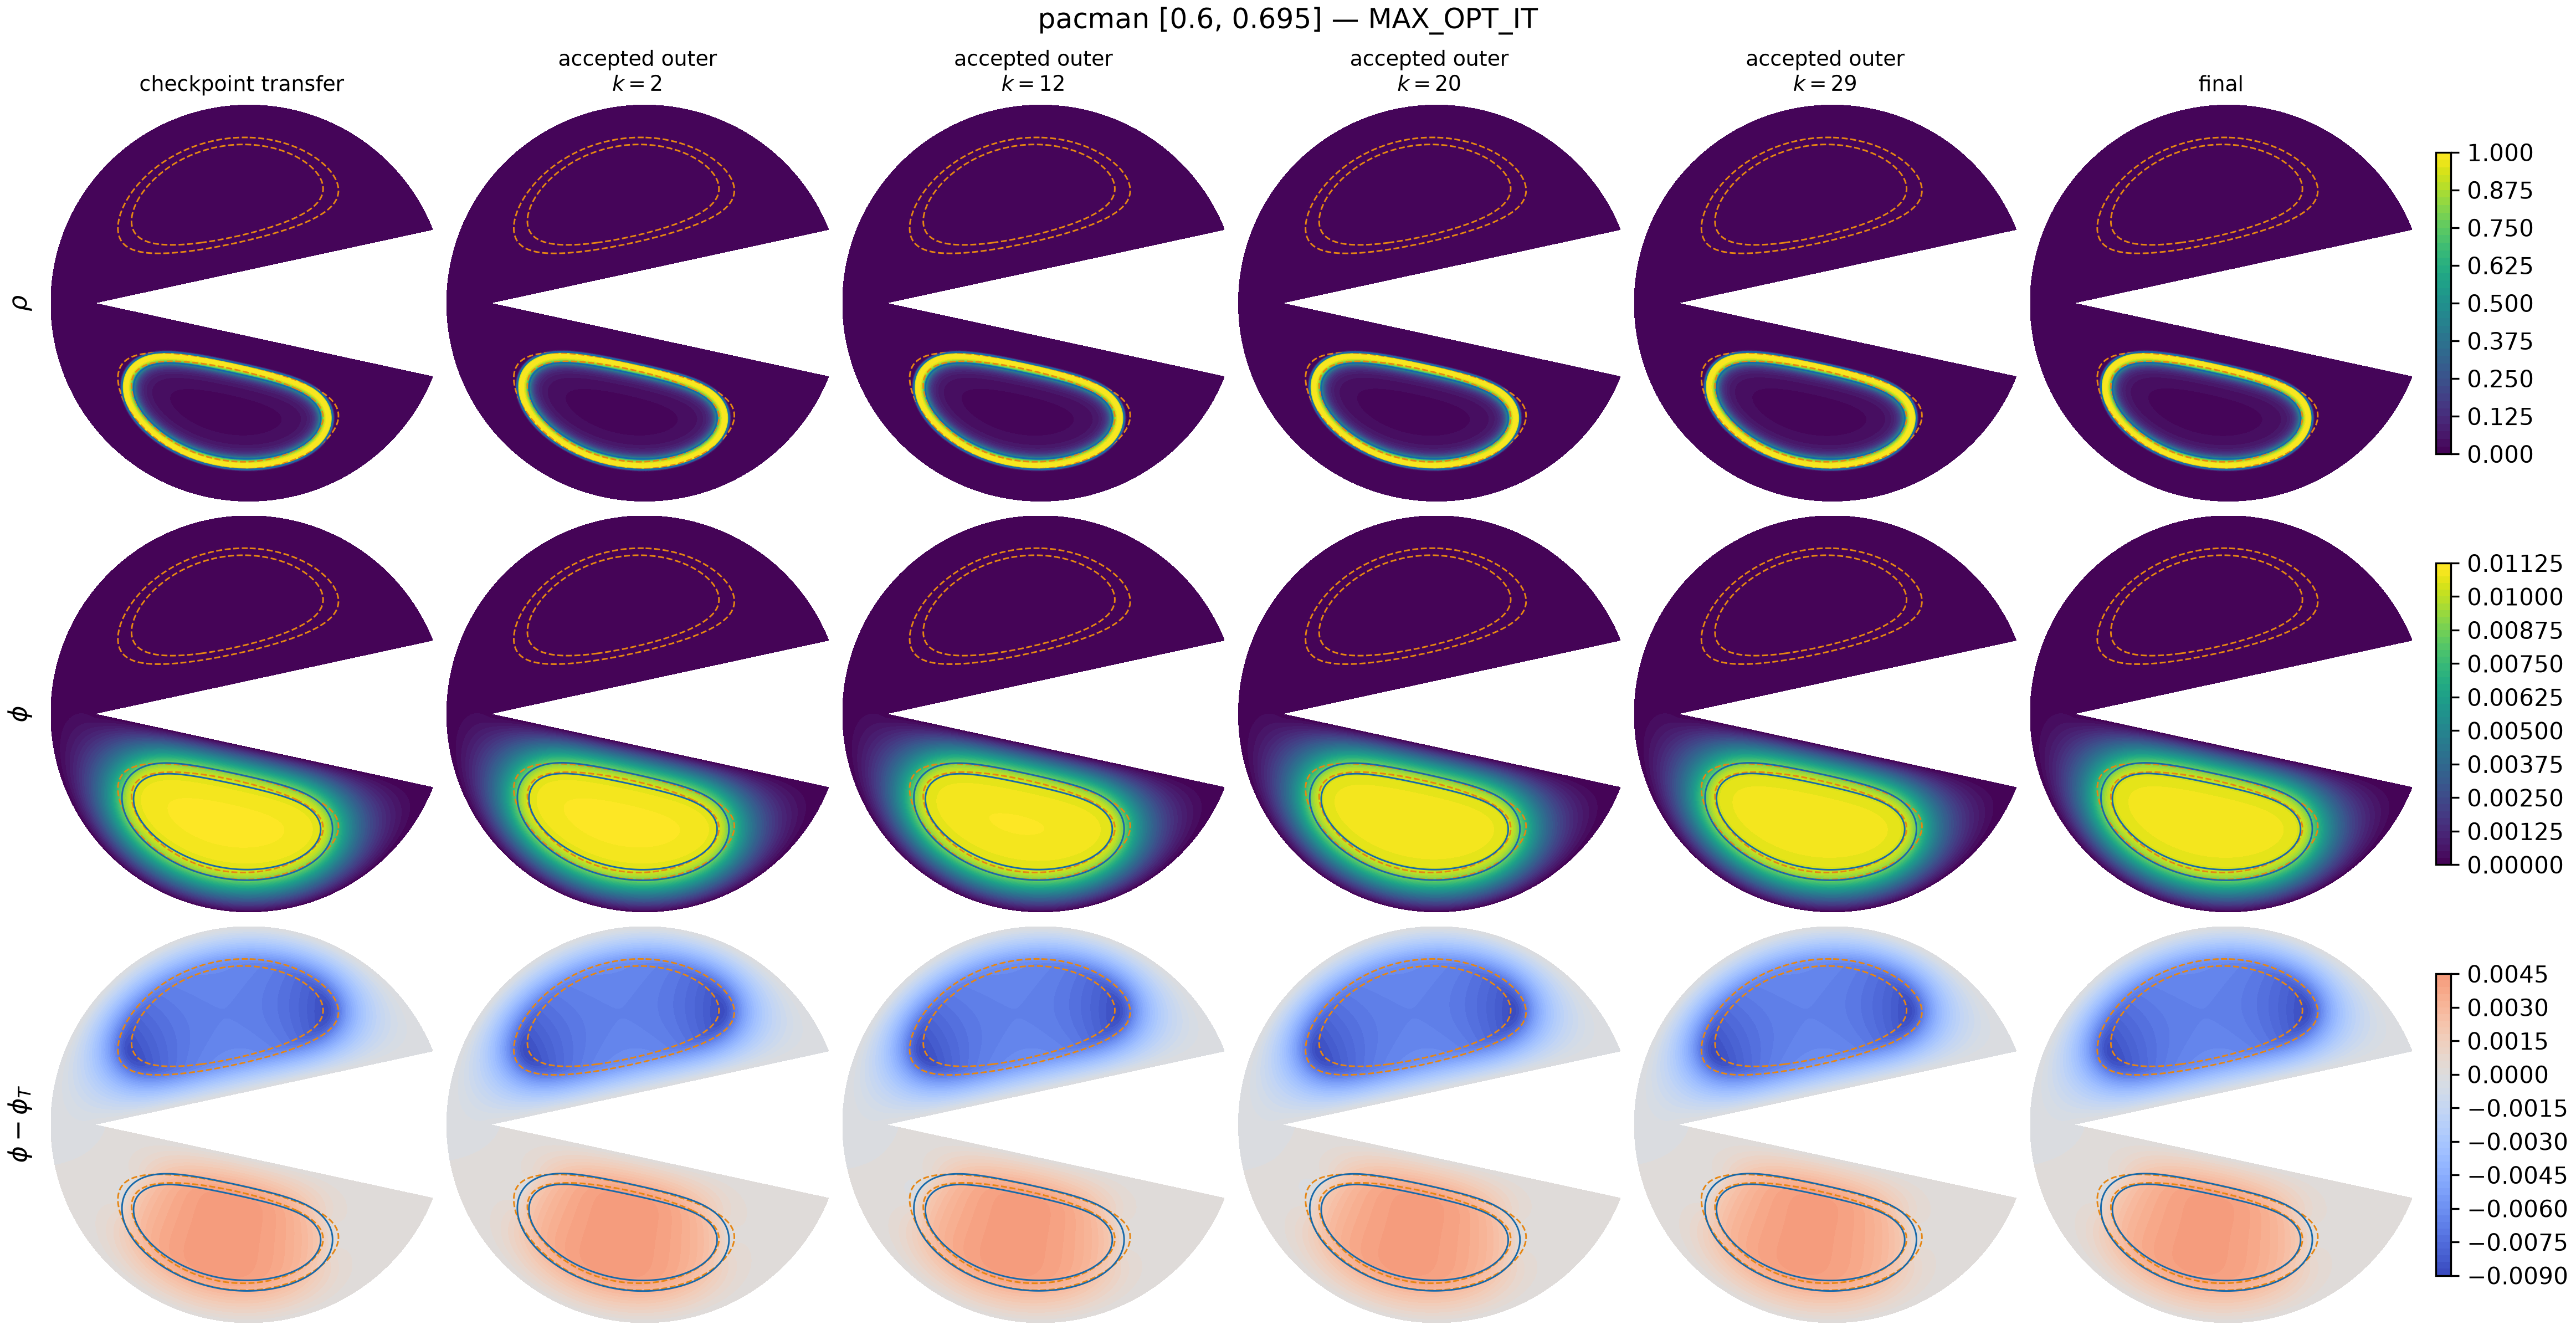
\includegraphics[width=0.97\linewidth]{figures/band_evolution_pacman_0p6_0p695.png}
\caption{Pacman equilibrium formation for torsion levels $[0.6,0.695]$: selected seed, intermediate homotopy, early and middle accepted states, late or restored-best state, and final projection; PDE-converged with a retained geometric plateau.  Orange dashed curves are the fixed target band and blue solid curves are the moving equilibrium band. Data status: actual.}
\label{fig:band-evolution-pacman}
\end{figure}
\end{landscape}

\begin{landscape}
\begin{figure}[tbp]
\centering
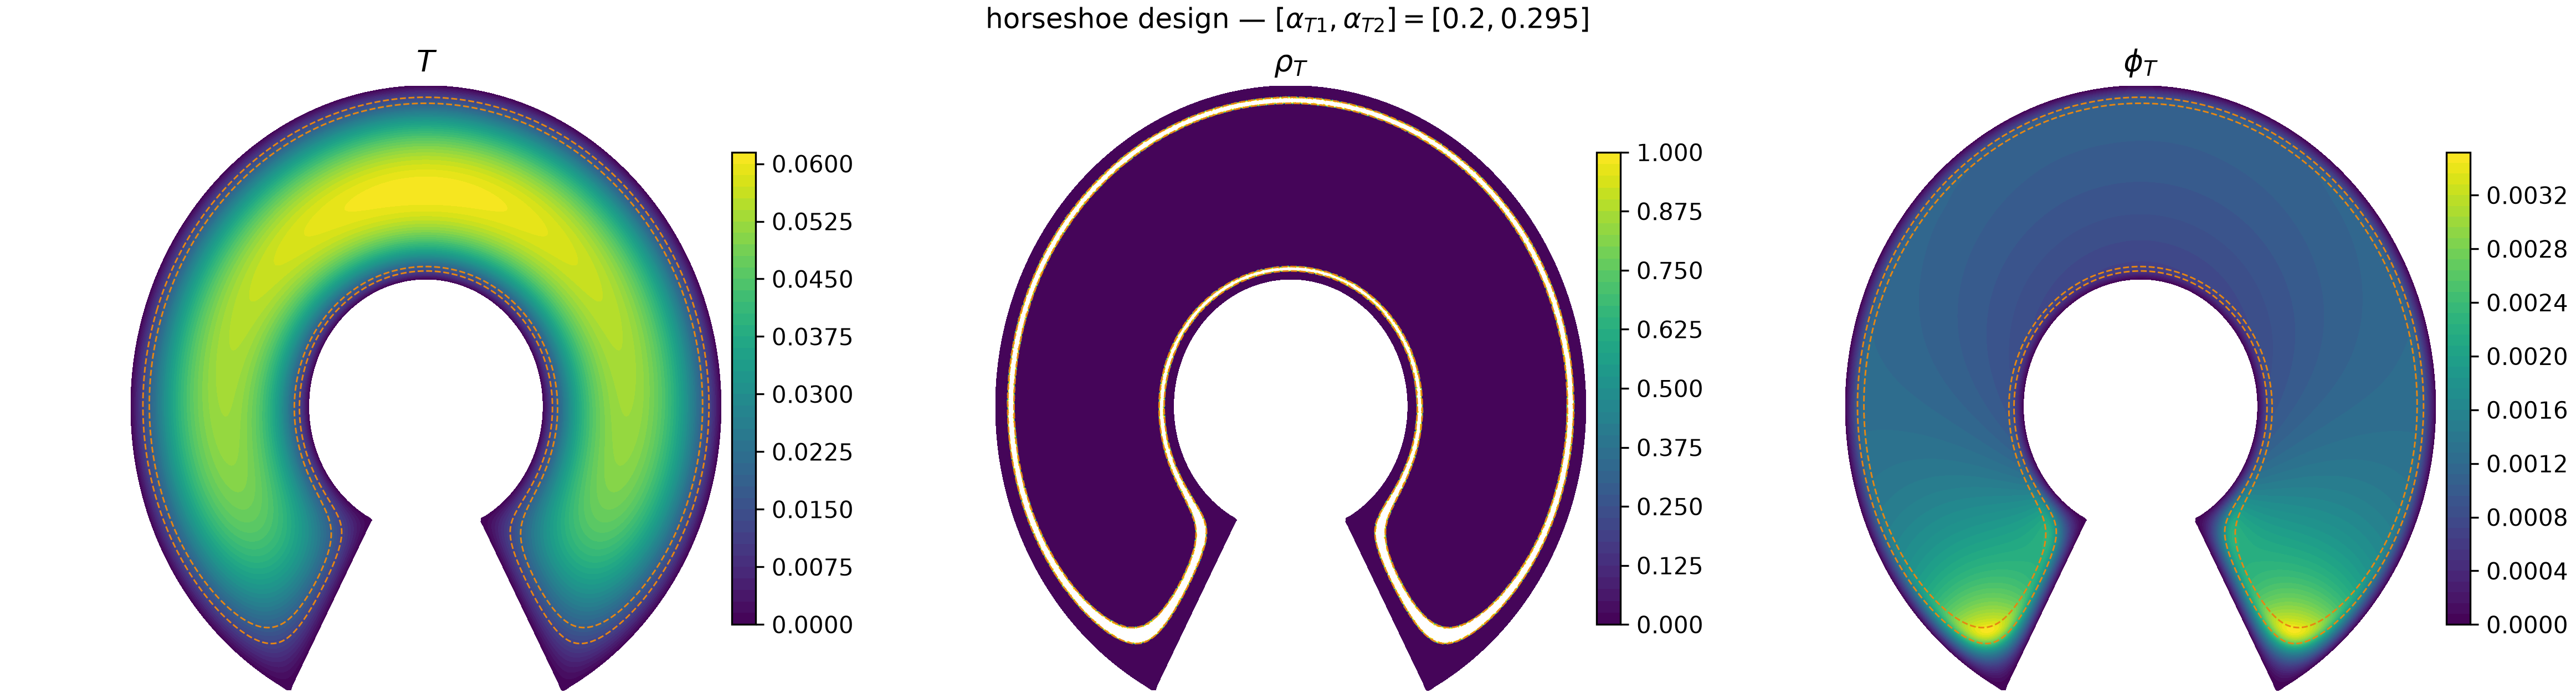
\includegraphics[width=0.97\linewidth]{figures/design_fields_horseshoe_0p2_0p295.png}
\caption{Horseshoe design fields for torsion levels $[0.2,0.295]$: torsion, target density, and target potential.  The design is shown once; orange dashed curves mark its fixed band boundaries. Data status: actual.}
\label{fig:design-fields-horseshoe}
\end{figure}
\end{landscape}

\begin{landscape}
\begin{figure}[tbp]
\centering
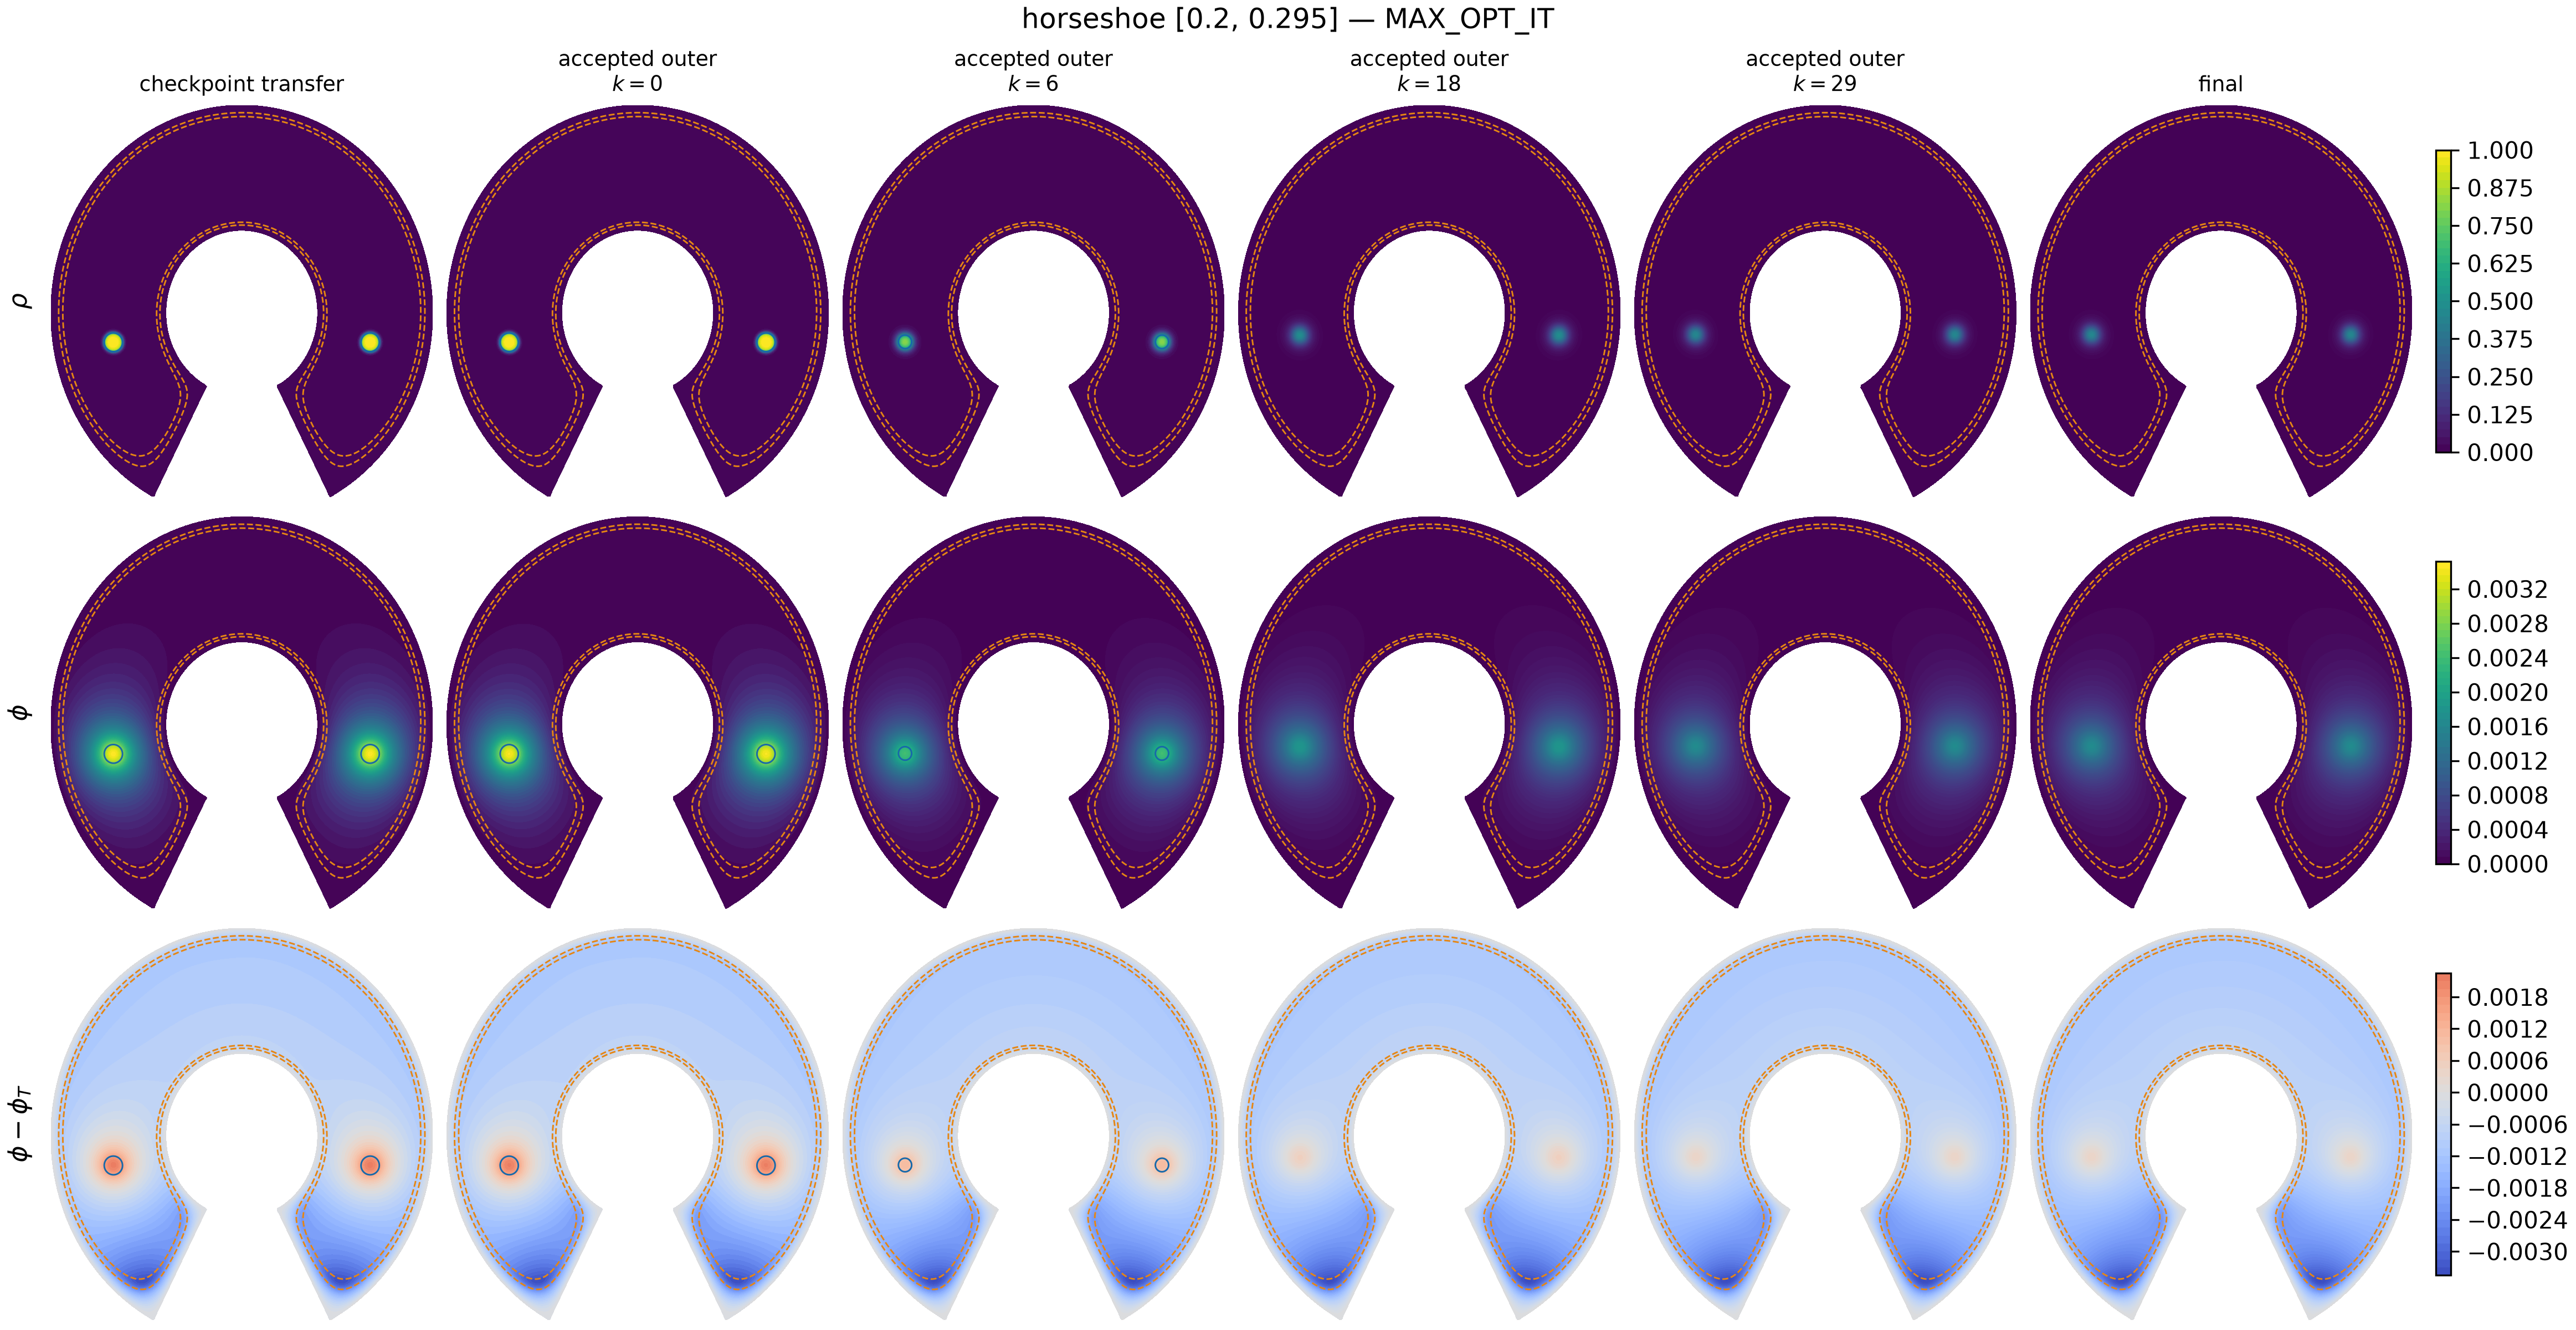
\includegraphics[width=0.97\linewidth]{figures/band_evolution_horseshoe_0p2_0p295.png}
\caption{Horseshoe equilibrium formation for torsion levels $[0.2,0.295]$: selected seed, intermediate homotopy, early and middle accepted states, late or restored-best state, and final projection; PDE-converged with a retained geometric plateau.  Orange dashed curves are the fixed target band and blue solid curves are the moving equilibrium band. Data status: actual.}
\label{fig:band-evolution-horseshoe}
\end{figure}
\end{landscape}

\begin{landscape}
\begin{figure}[tbp]
\centering
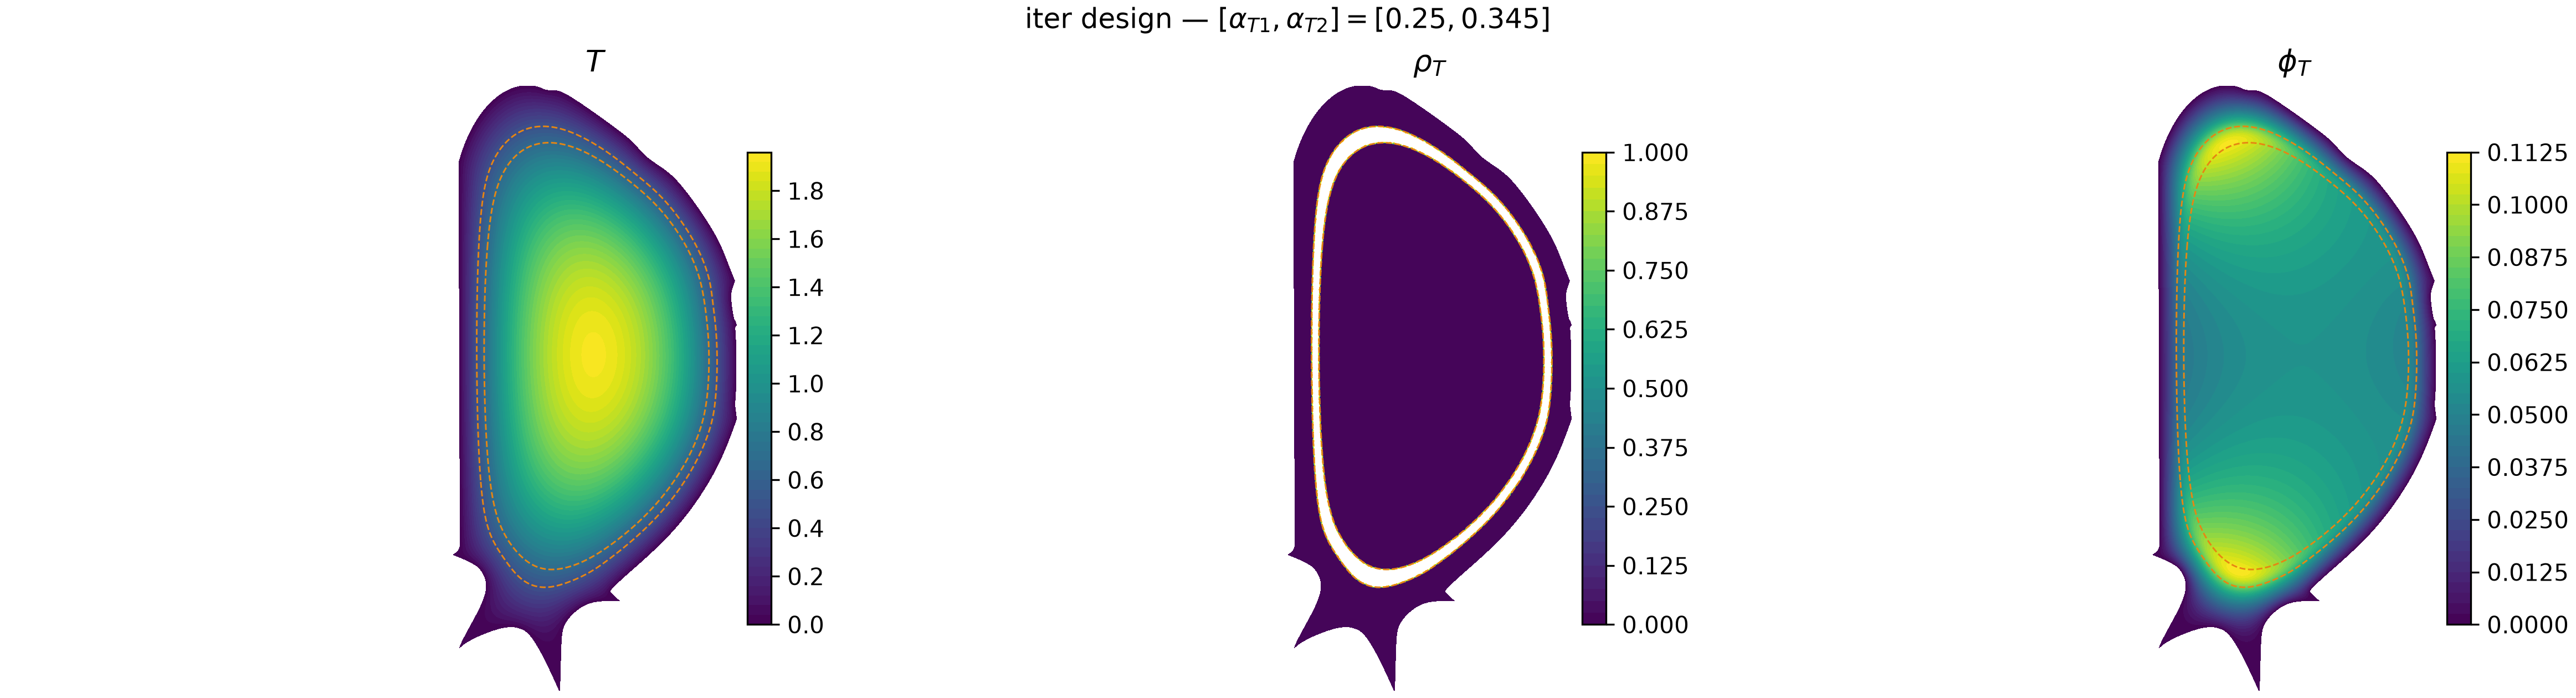
\includegraphics[width=0.97\linewidth]{figures/design_fields_iter_0p25_0p345.png}
\caption{Iter design fields for torsion levels $[0.25,0.345]$: torsion, target density, and target potential.  The design is shown once; orange dashed curves mark its fixed band boundaries. Data status: actual.}
\label{fig:design-fields-iter}
\end{figure}
\end{landscape}

\begin{landscape}
\begin{figure}[tbp]
\centering
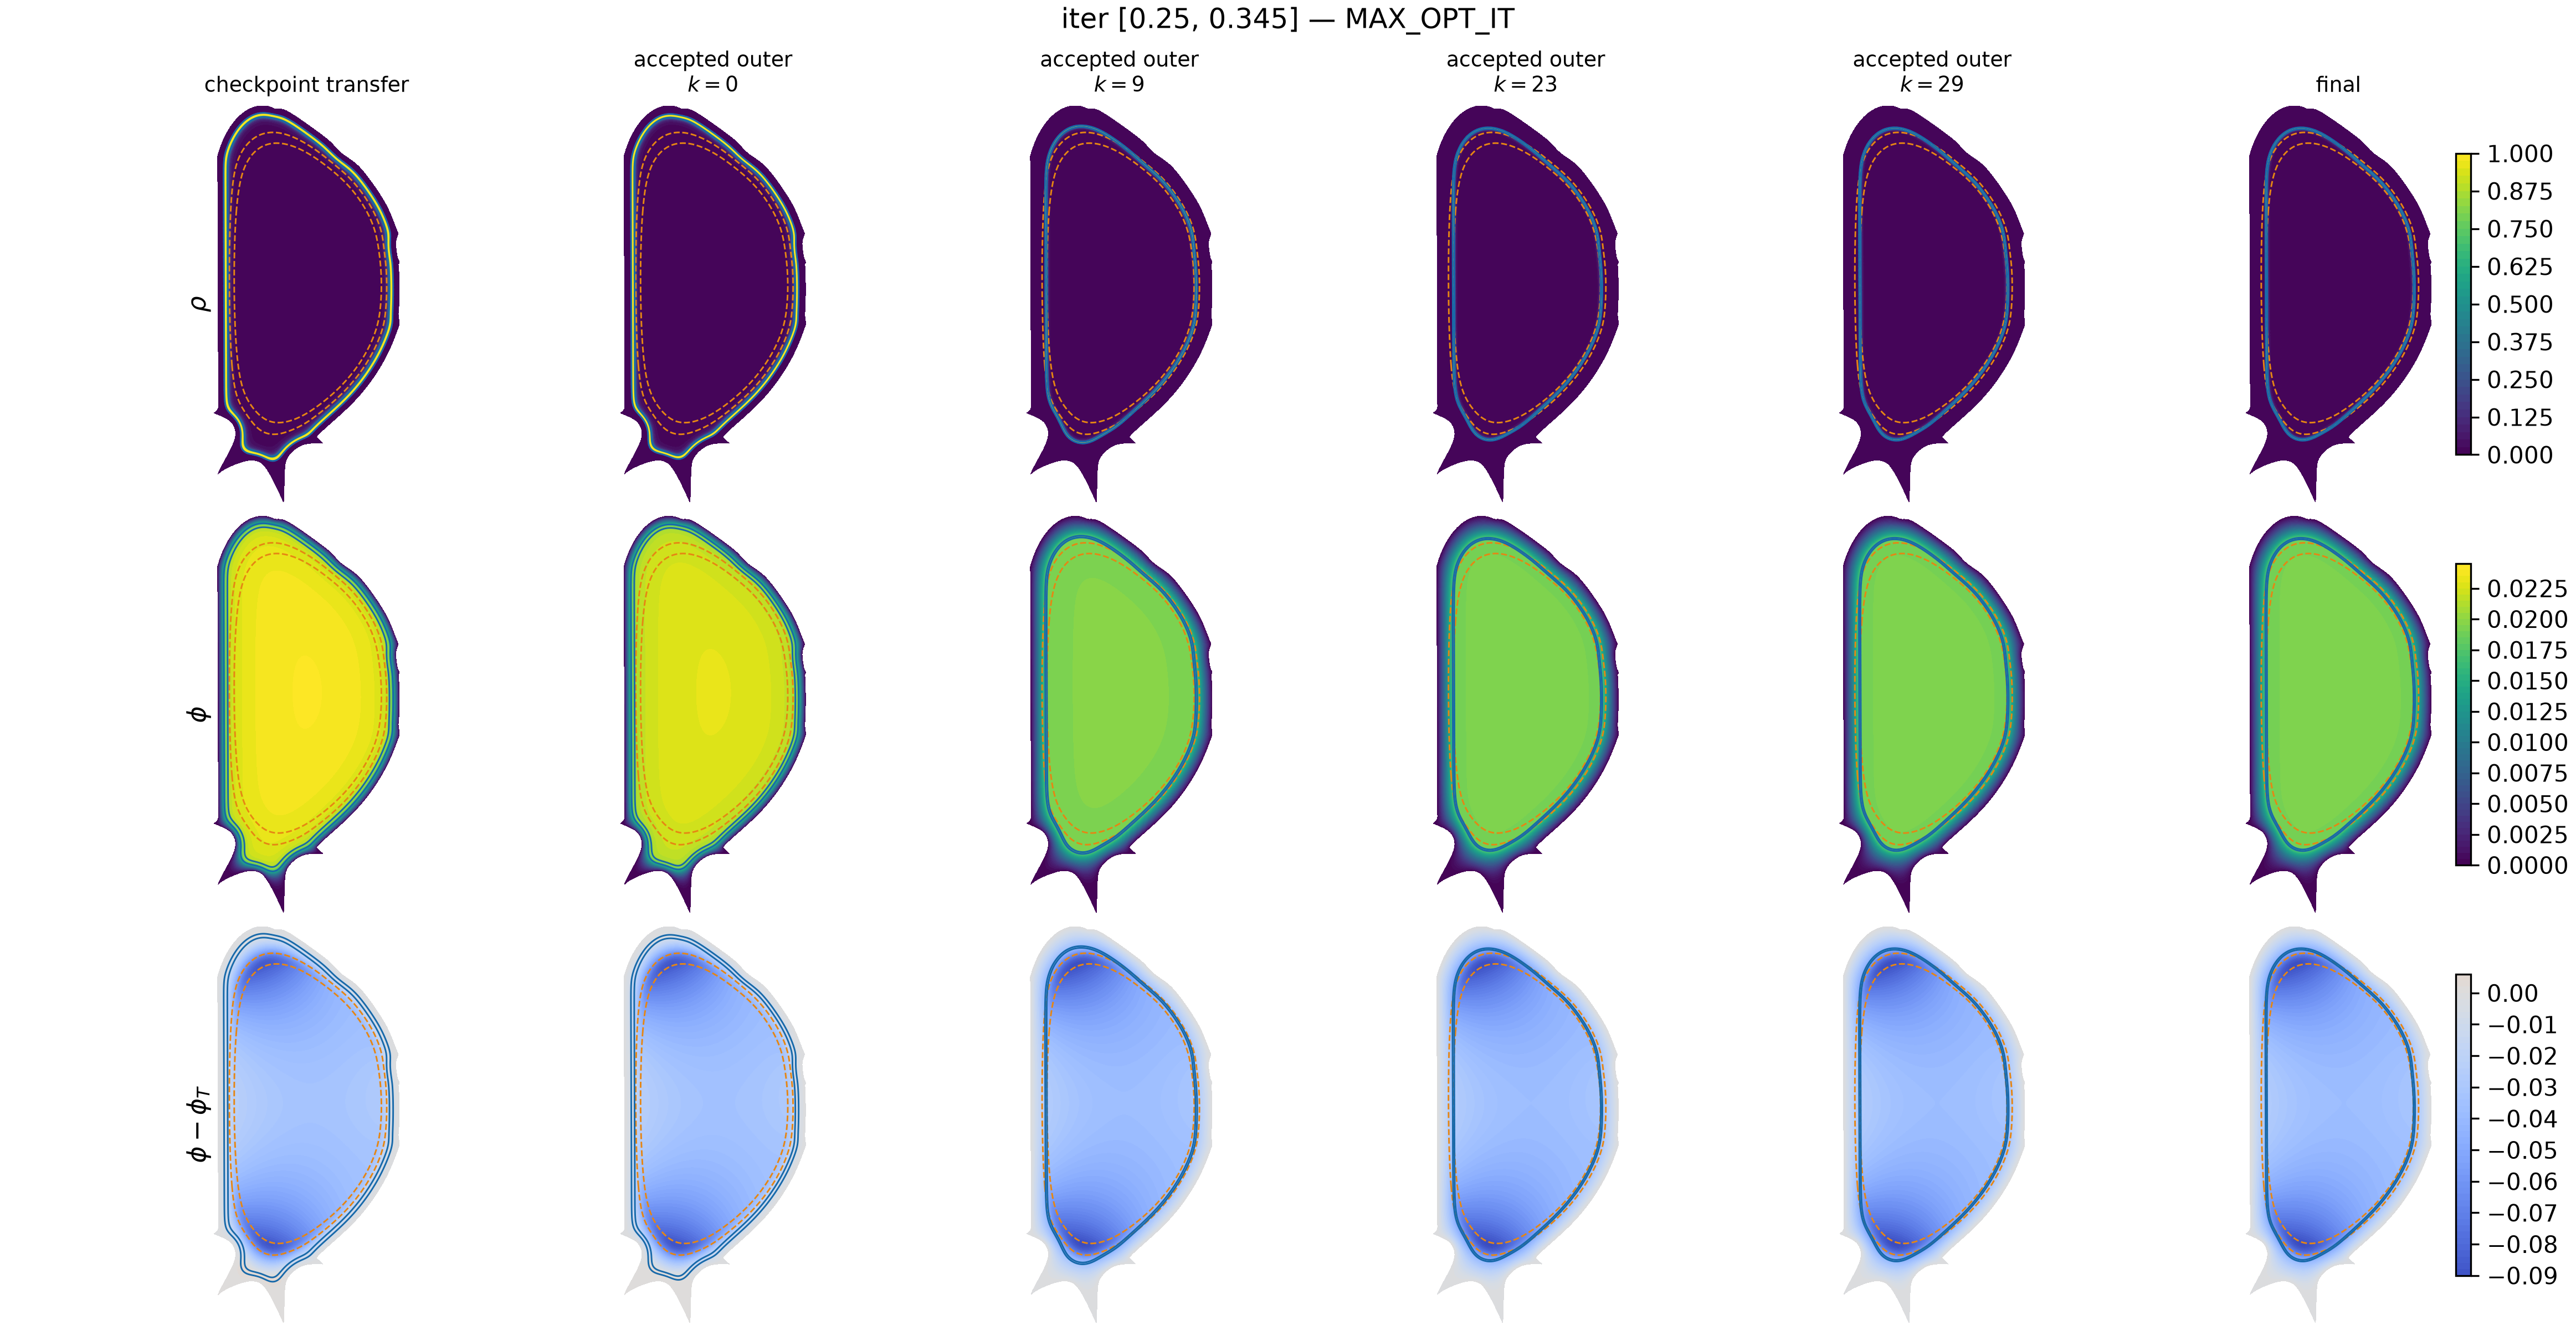
\includegraphics[width=0.97\linewidth]{figures/band_evolution_iter_0p25_0p345.png}
\caption{Iter equilibrium formation for torsion levels $[0.25,0.345]$: selected seed, intermediate homotopy, early and middle accepted states, late or restored-best state, and final projection; PDE-converged with retained capped trials.  Orange dashed curves are the fixed target band and blue solid curves are the moving equilibrium band. Data status: actual.}
\label{fig:band-evolution-iter}
\end{figure}
\end{landscape}

\clearpage

\begin{figure}[tbp]
\centering
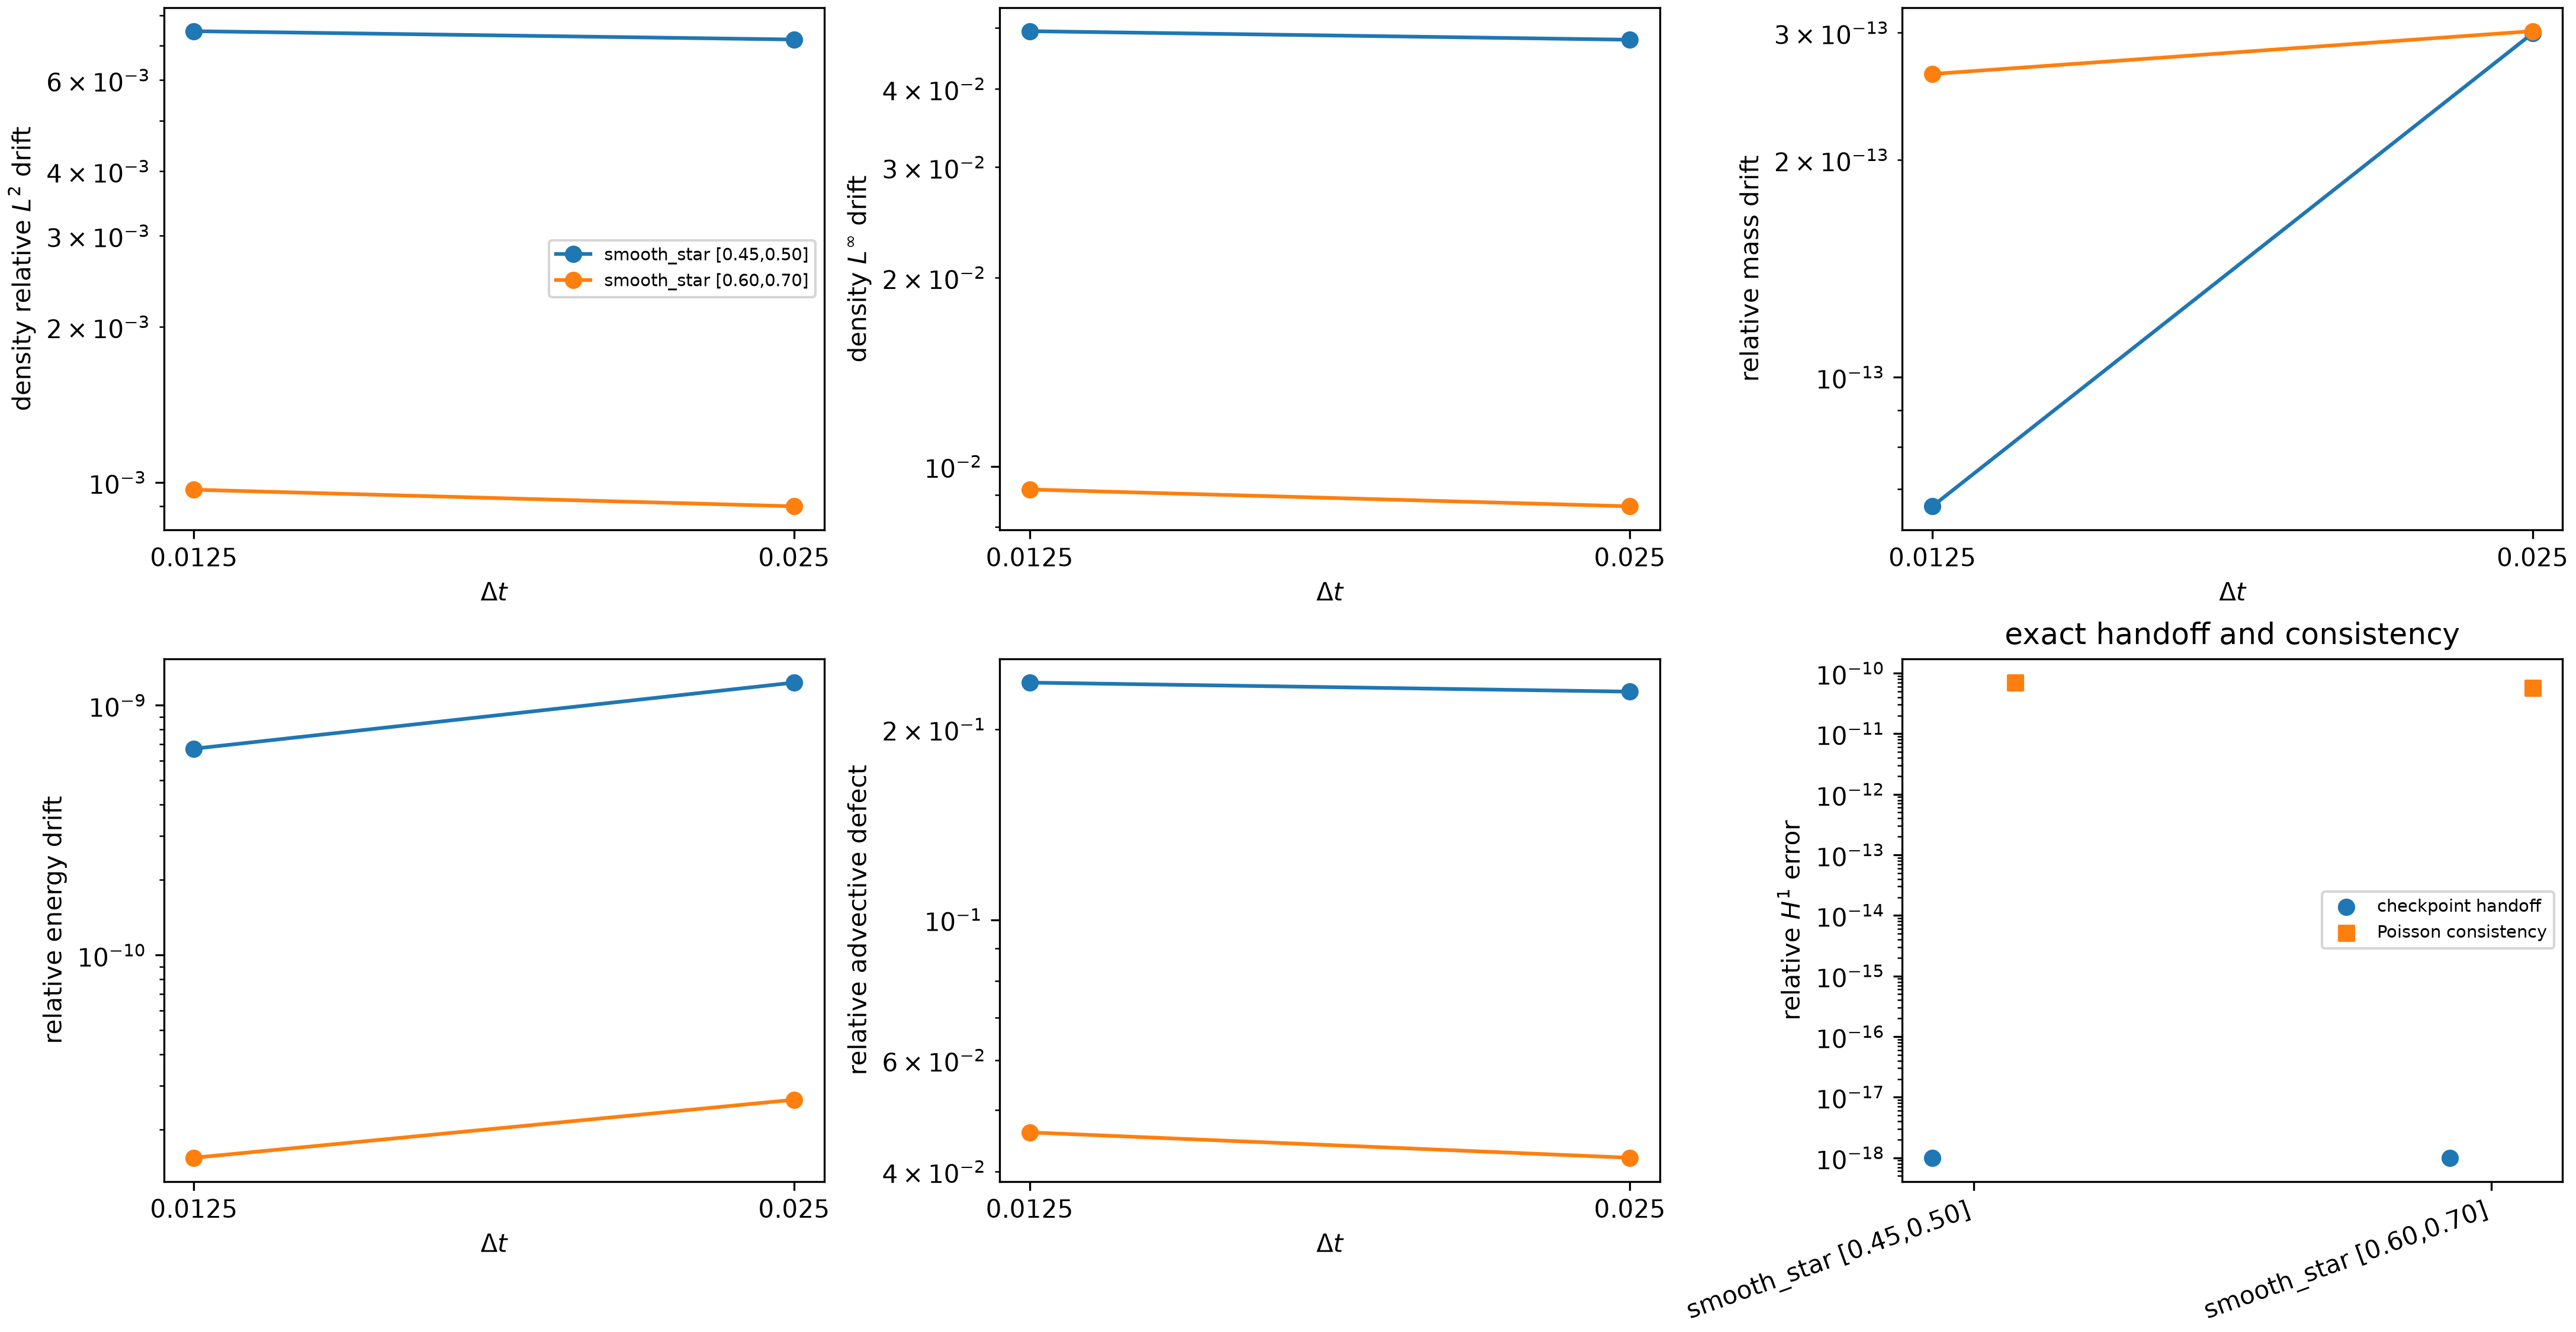
\includegraphics[width=0.88\linewidth]{figures/guiding_center_stationarity.png}
\caption{Guiding-center stationarity and timestep sensitivity. Data status: actual.}
\label{fig:stationarity}
\end{figure}

\paragraph{High-resolution horseshoe confirmation.}
For the horseshoe target band $[0.35,0.50]\,T_{\max}$, the calibrated P4
mesh contains $589\,779$ global degrees of freedom.  Starting from the same
candidate-119 initialization used by the lower-resolution experiment, the
reduced optimizer accepted 17 threshold steps and reached
$\lVert R\rVert_2=1.39\times10^{-13}$ at
$(c_{1,\phi},c_{2,\phi})=(2.869885,3.352889)\times10^{-3}$.
The threshold loop reached its 20-step cap, so this result is classified as a
PDE-converged geometric plateau rather than strict full-band convergence;
the certified leakage is nevertheless $1.36\%$ of the target area.

\begin{figure}[tbp]
\centering
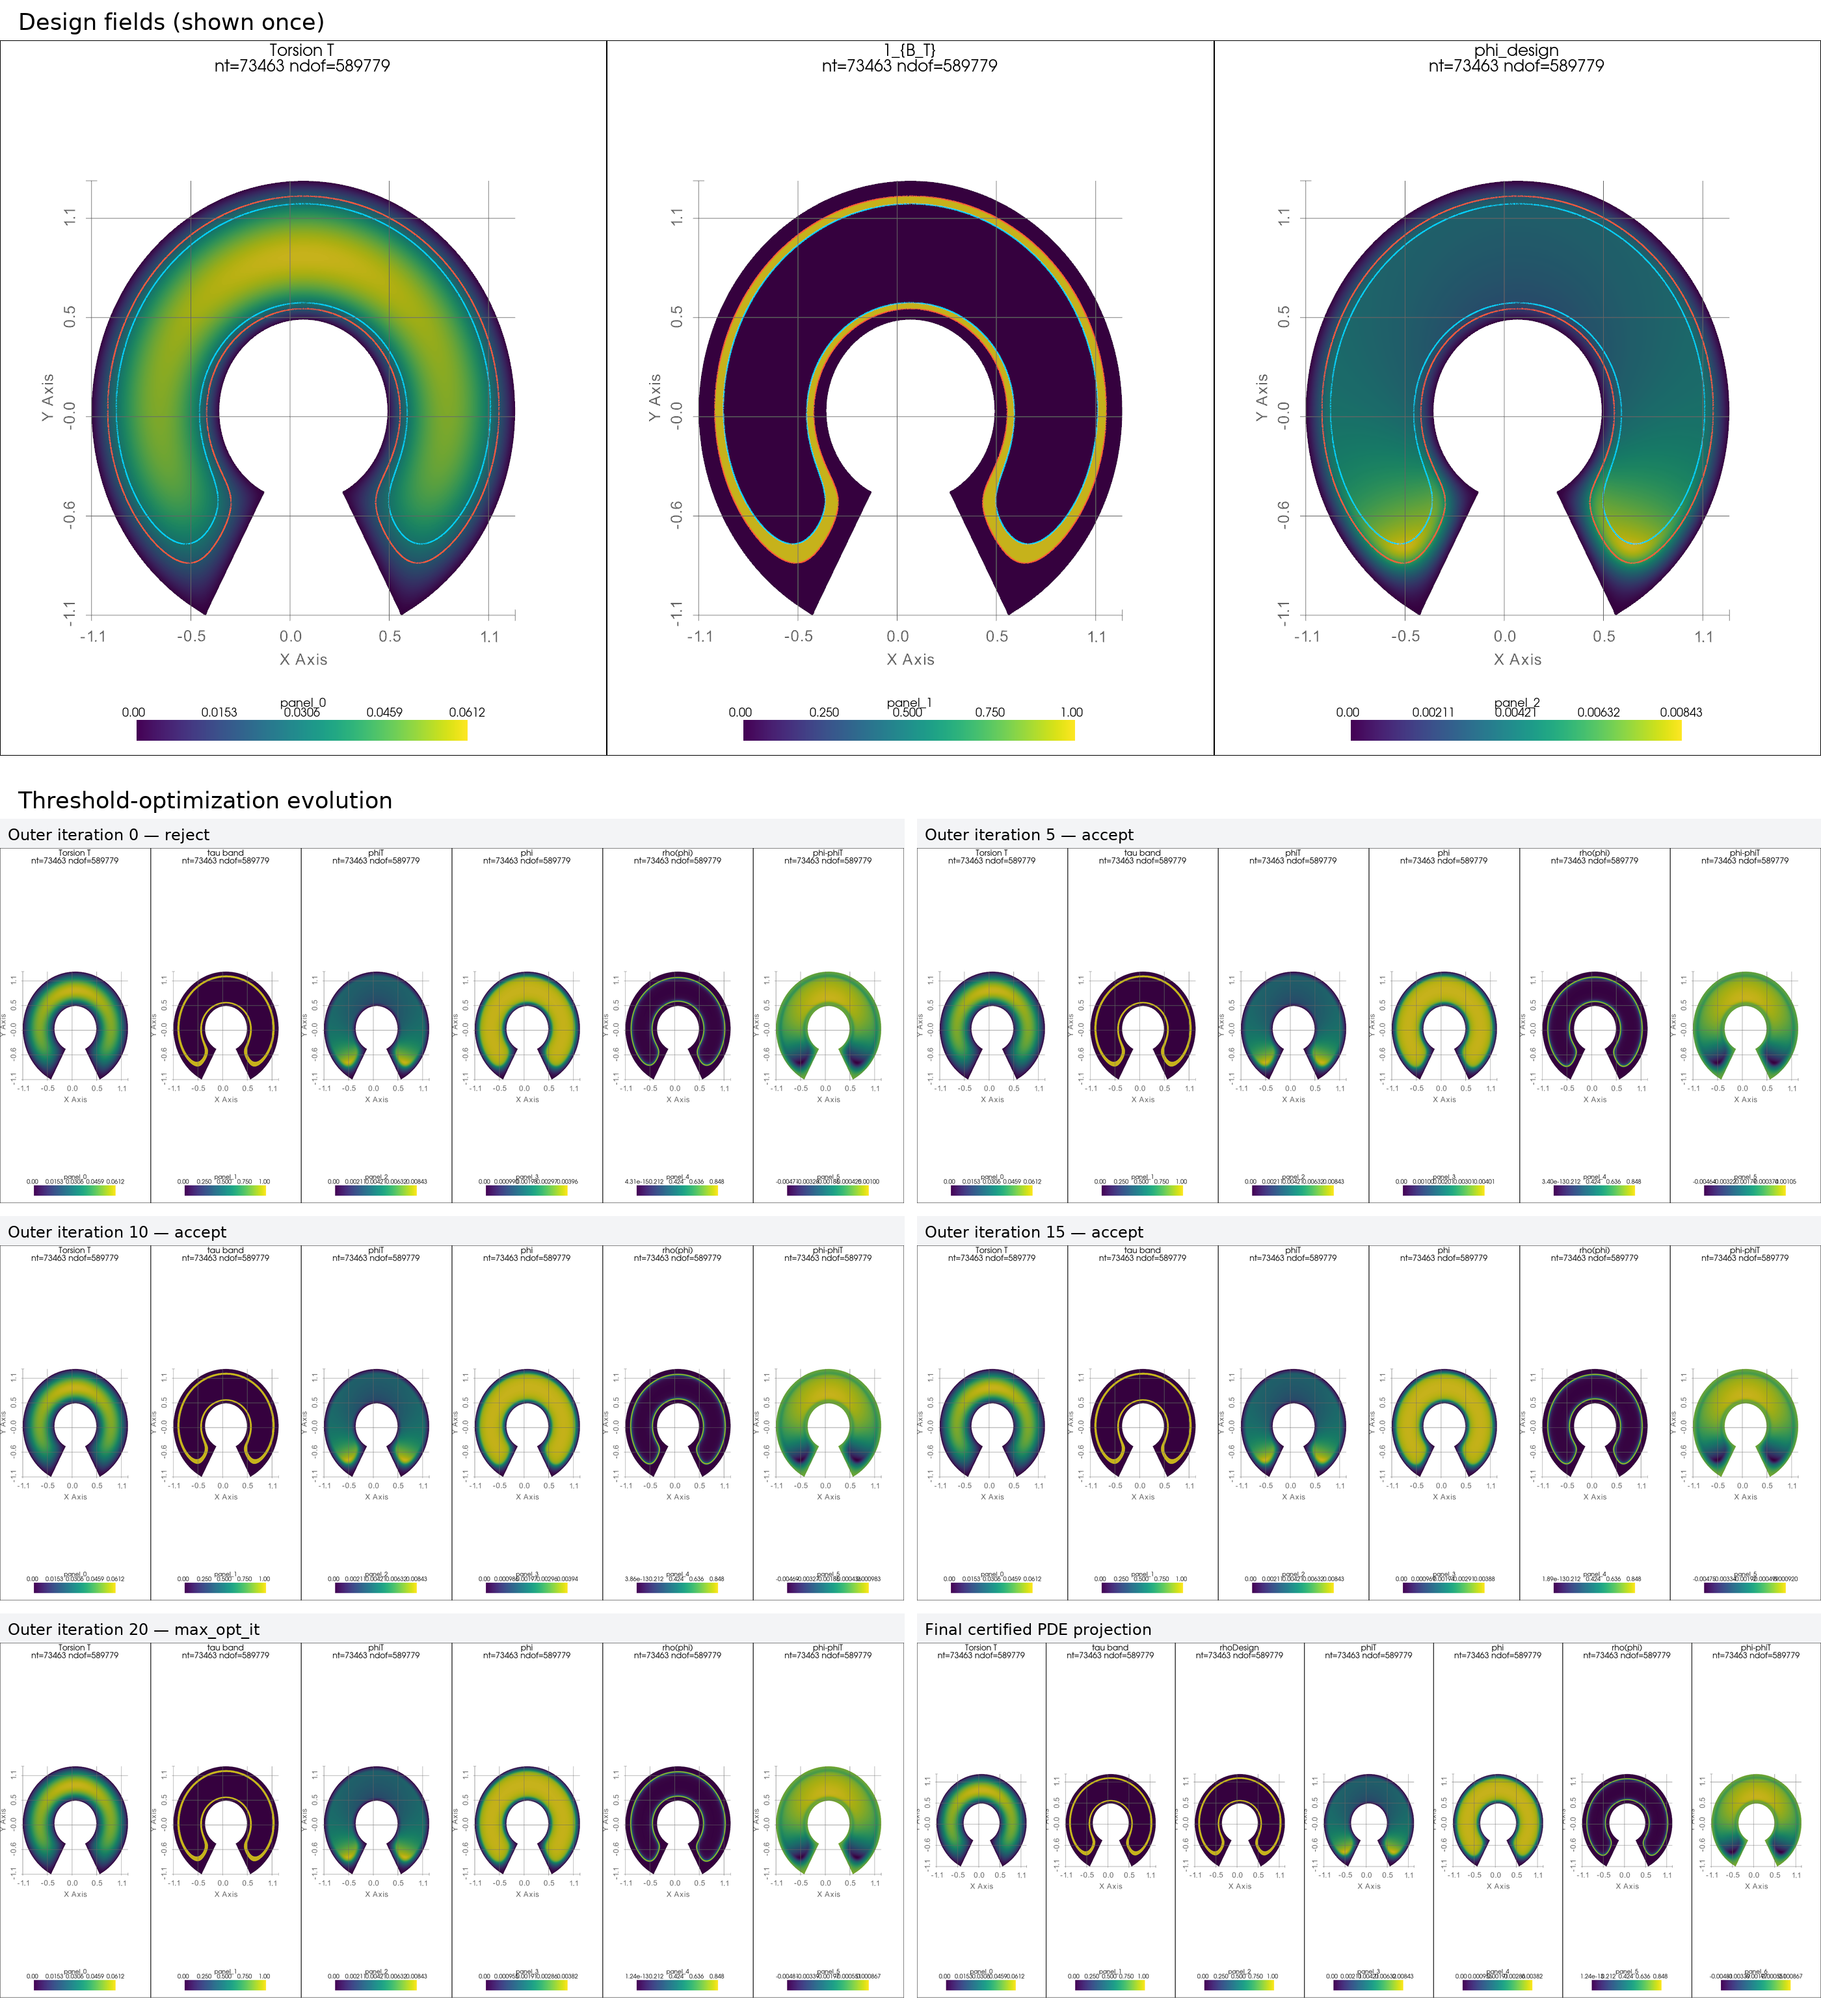
\includegraphics[width=0.97\linewidth,height=0.78\textheight,keepaspectratio]{figures/horseshoe_0p35_0p50_dof600000_optimizer_storyboard.png}
\caption{High-resolution horseshoe threshold optimization.  The fixed design
fields are shown once above the selected outer iterates and final projection.
All panels use a complete eight-rank gather on rank zero; mesh edges are
suppressed.  The alternating late states expose the leakage--missing-area
threshold plateau. Data status: actual.}
\label{fig:horseshoe-600k-optimizer}
\end{figure}

\begin{figure}[tbp]
\centering
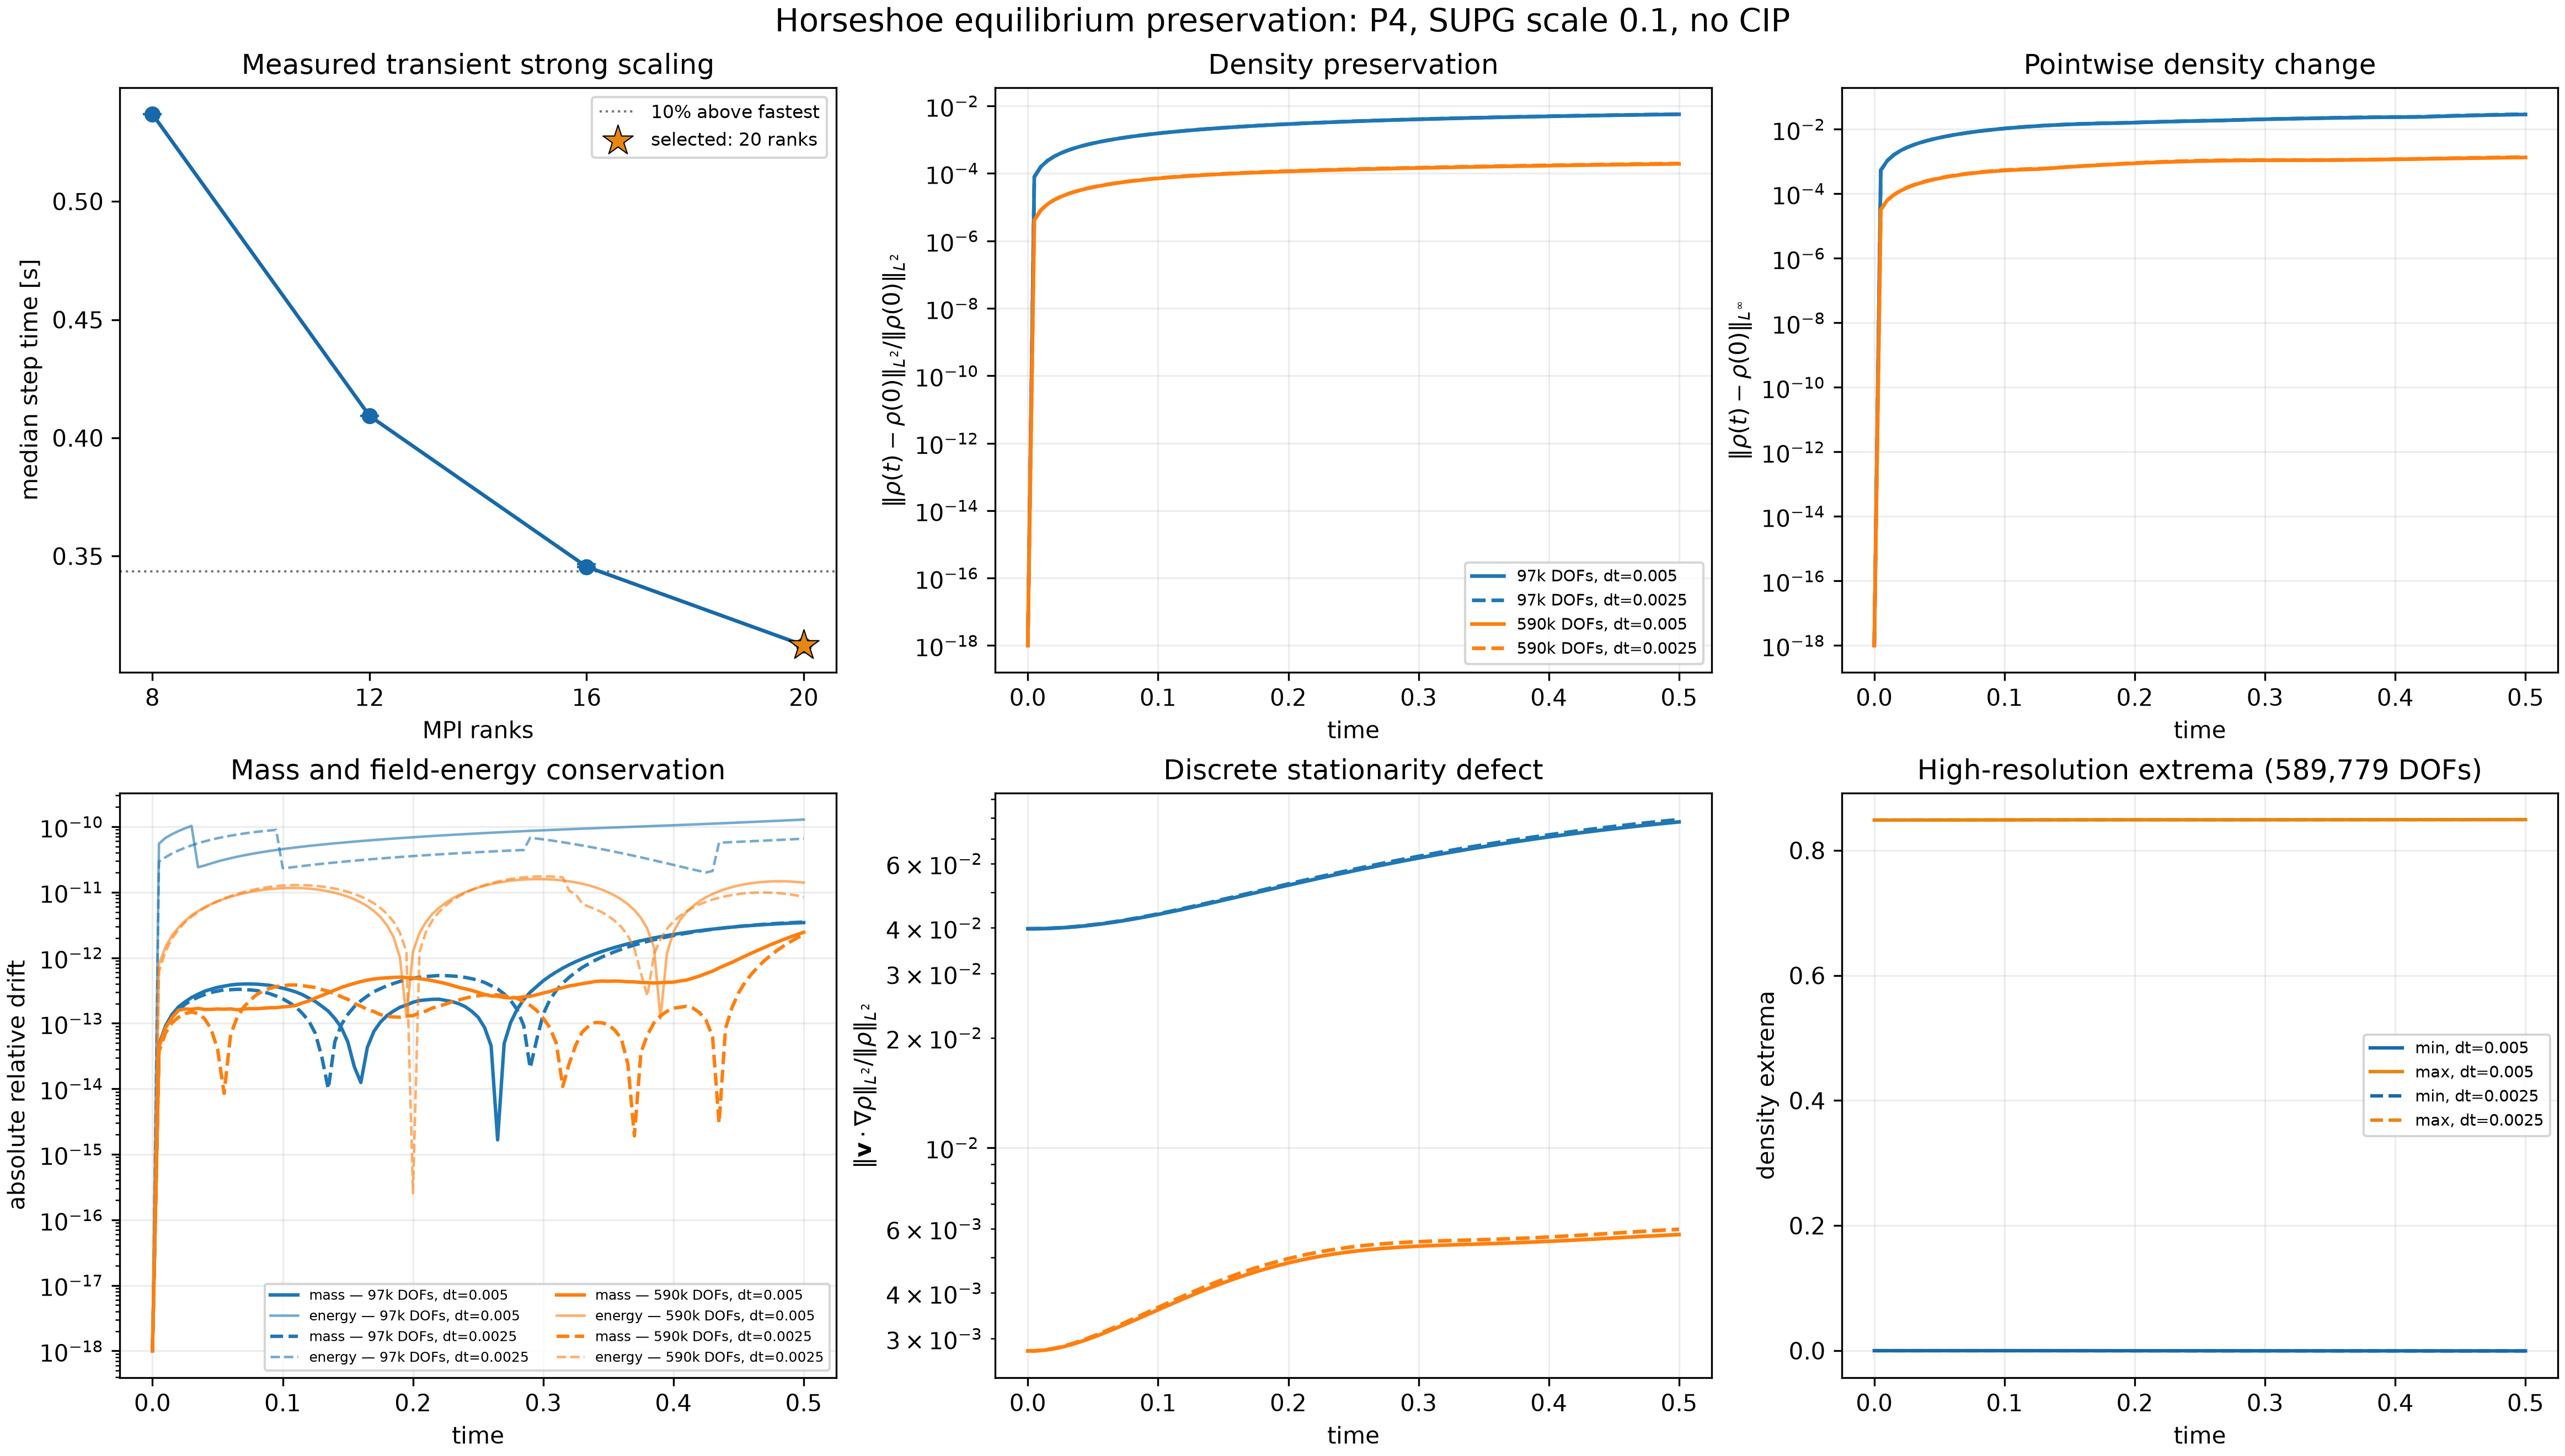
\includegraphics[width=0.98\linewidth]{figures/horseshoe_0p35_0p50_stationarity_dof_comparison.png}
\caption{Resolution and timestep study for the horseshoe equilibrium with
SUPG scale $0.1$ and no CIP.  At $T=0.5$, the $589\,779$-DOF solution changes
by $1.92\times10^{-4}$ in relative $L^2$ density and
$1.34\times10^{-3}$ in $L^\infty$ for $\Delta t=0.005$; halving the
timestep gives $1.98\times10^{-4}$ and $1.38\times10^{-3}$.
The nearly unchanged values identify a spatial/discrete floor, while the
roughly 30-fold improvement over the $97\,141$-DOF run demonstrates
resolution-dependent stationarity.  Mass and energy remain conserved to
$2.5\times10^{-12}$ and $1.4\times10^{-11}$, respectively. Data status: actual.}
\label{fig:horseshoe-stationarity-resolution}
\end{figure}

\begin{figure}[tbp]
\centering
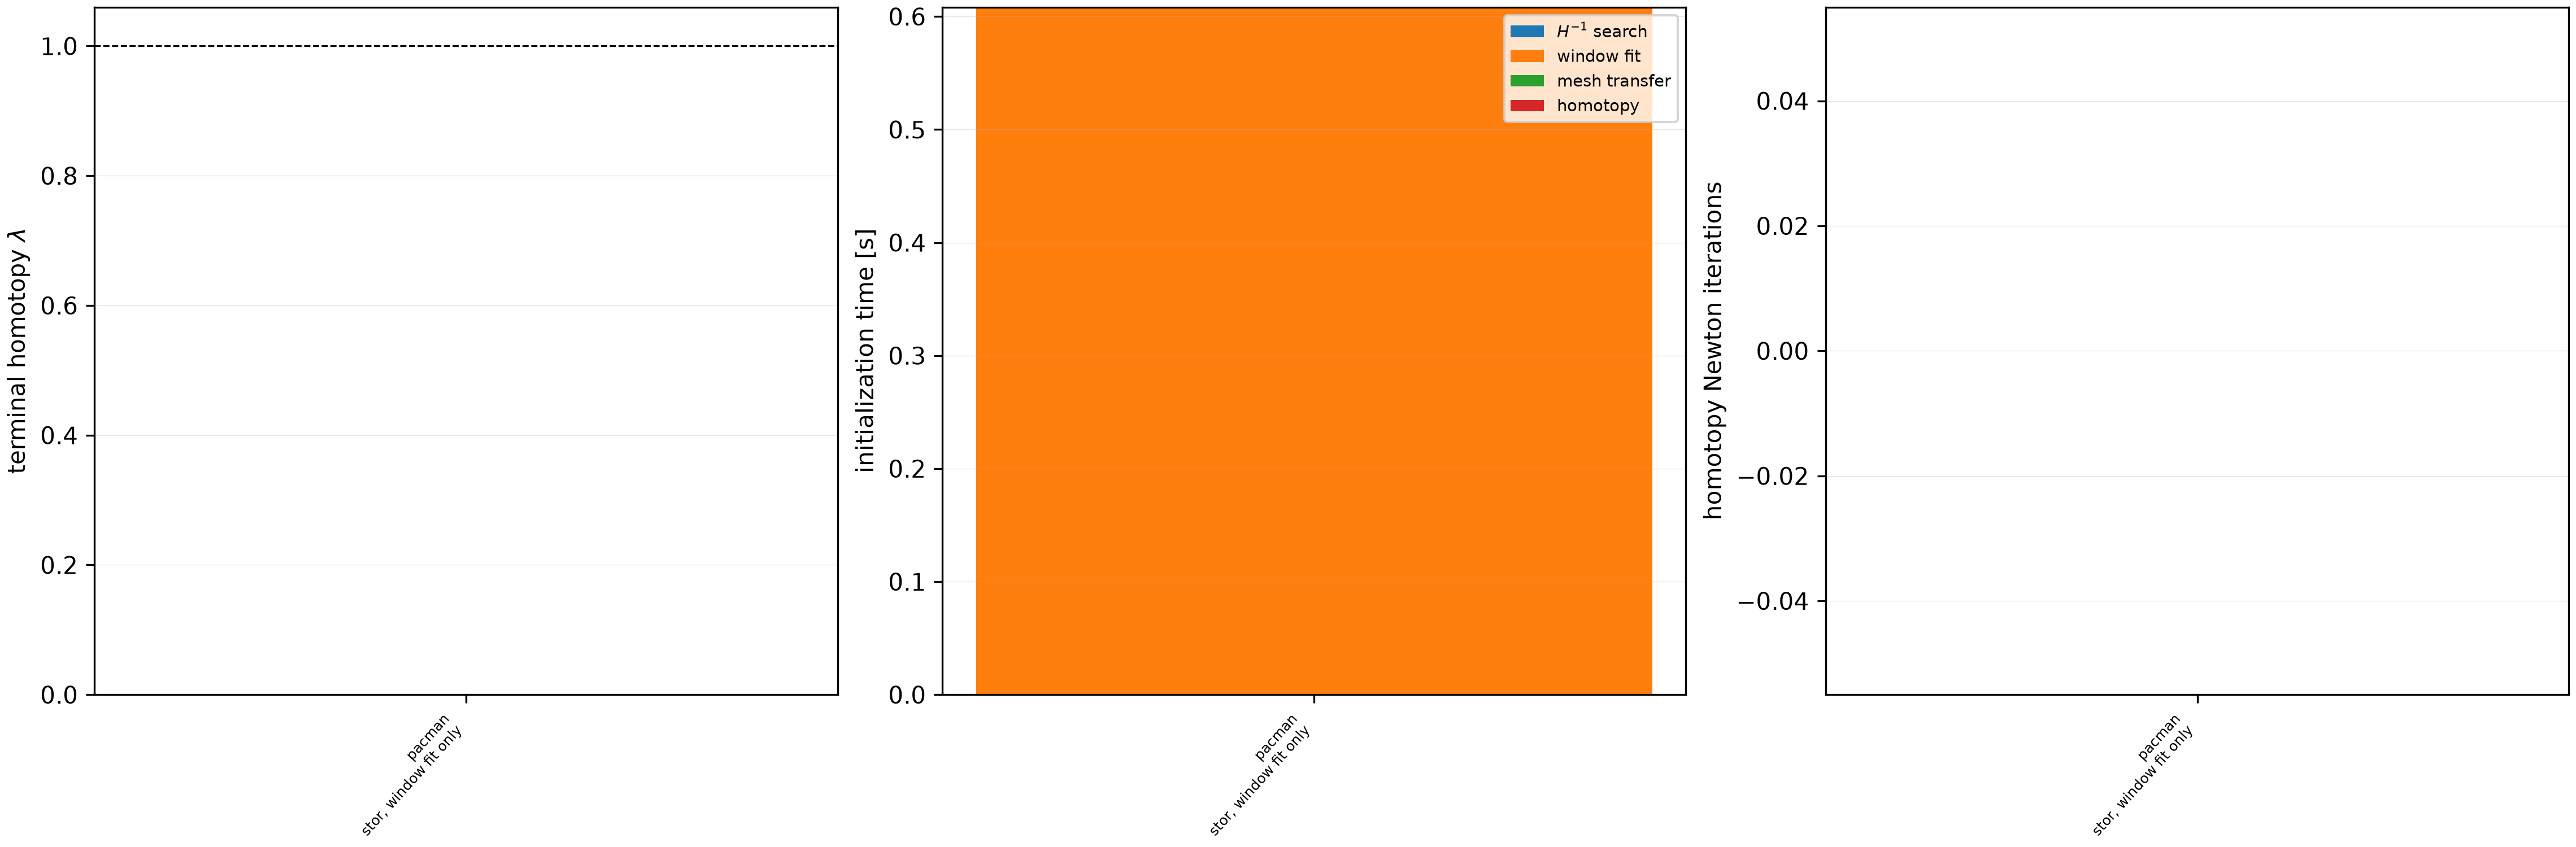
\includegraphics[width=0.88\linewidth]{figures/initialization_homotopy_summary.png}
\caption{Automatic initialization comparison: original and value-only fast H-minus-one searches, same-run window-fit fallback, continuation success, and nonlinear work. Data status: partial.}
\label{fig:initialization}
\end{figure}

\begin{figure}[tbp]
\centering
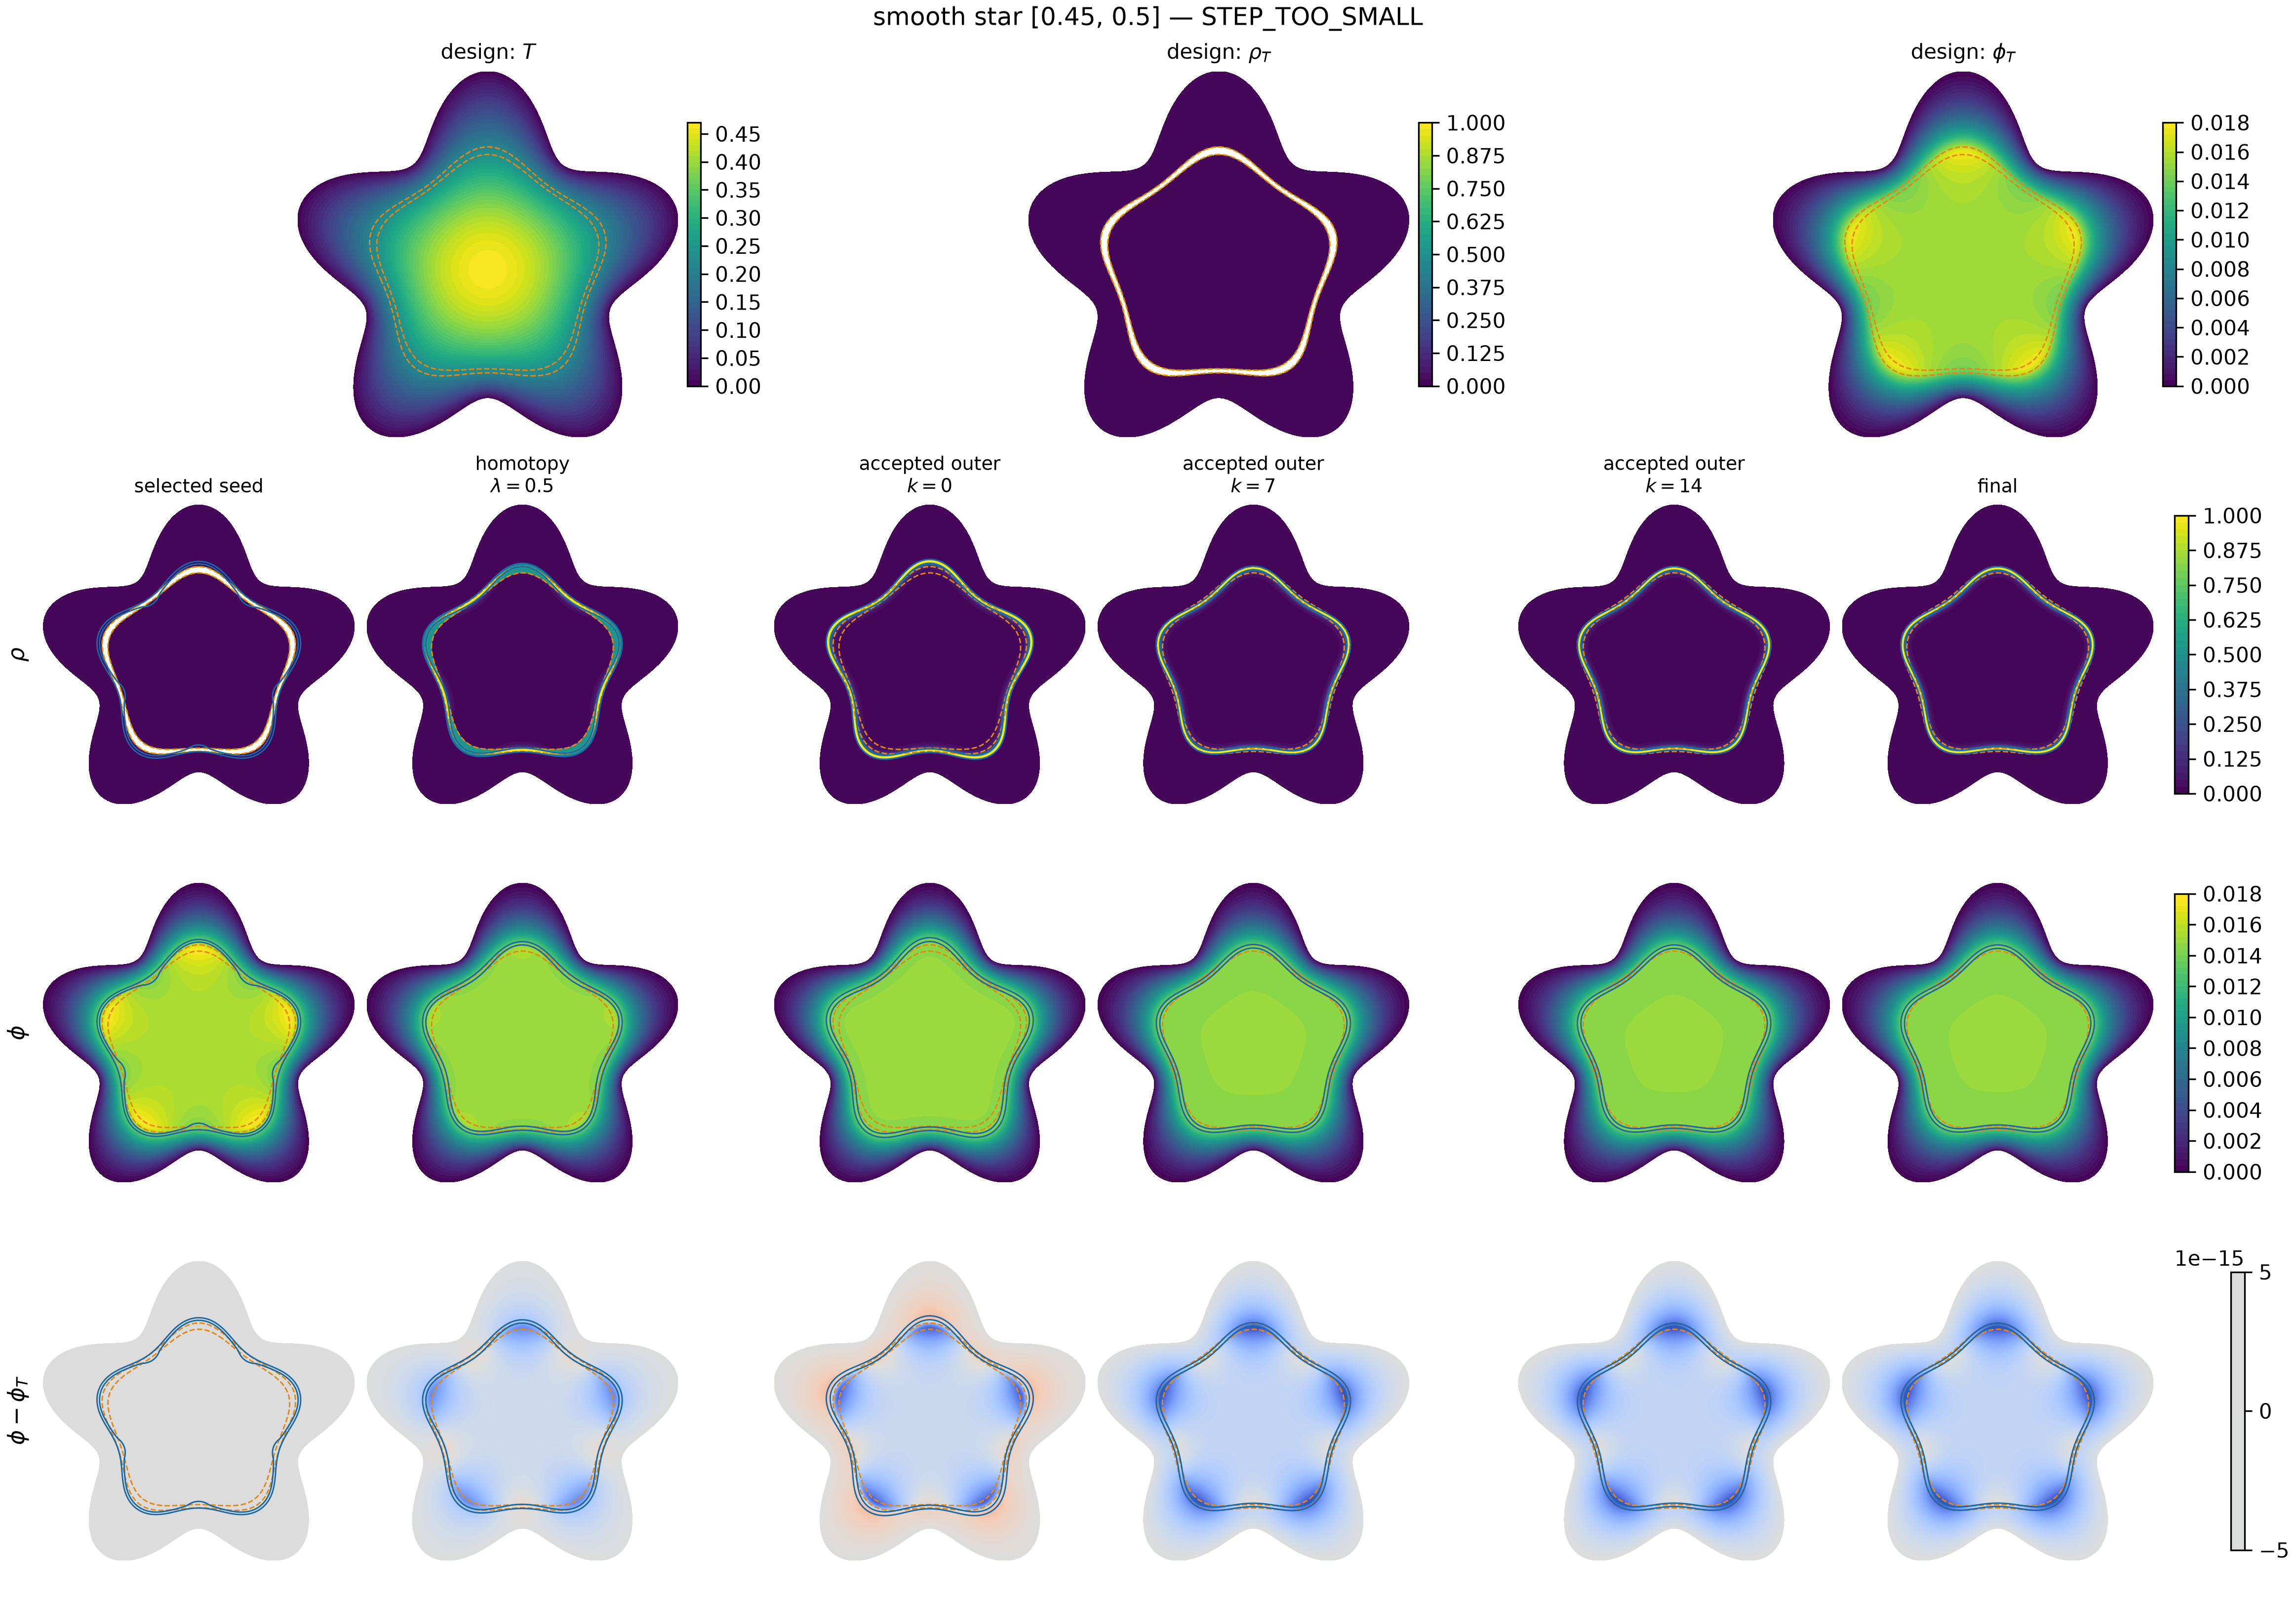
\includegraphics[width=0.88\linewidth]{figures/failed_band_evolution_000_smooth_star_0p45_0p5_trajectory-smooth_star-4ee334333e4c.png}
\caption{Supplemental failed/partial trajectory evidence for smooth star at torsion levels $[0.45,0.5]$ (case trajectory-smooth\_star-4ee334333e4c; state=completed; classification=geometrically\_unsuccessful\_pde\_converged). The case is retained regardless of PDE or geometric success. Orange dashed curves are the fixed target band and blue solid curves are the moving equilibrium band; when state recovery is impossible, the PNG records the reason. Data status: actual.}
\label{fig:failed-storyboard-trajectory-smooth-star-4ee334333e4c}
\end{figure}

\begin{figure}[tbp]
\centering
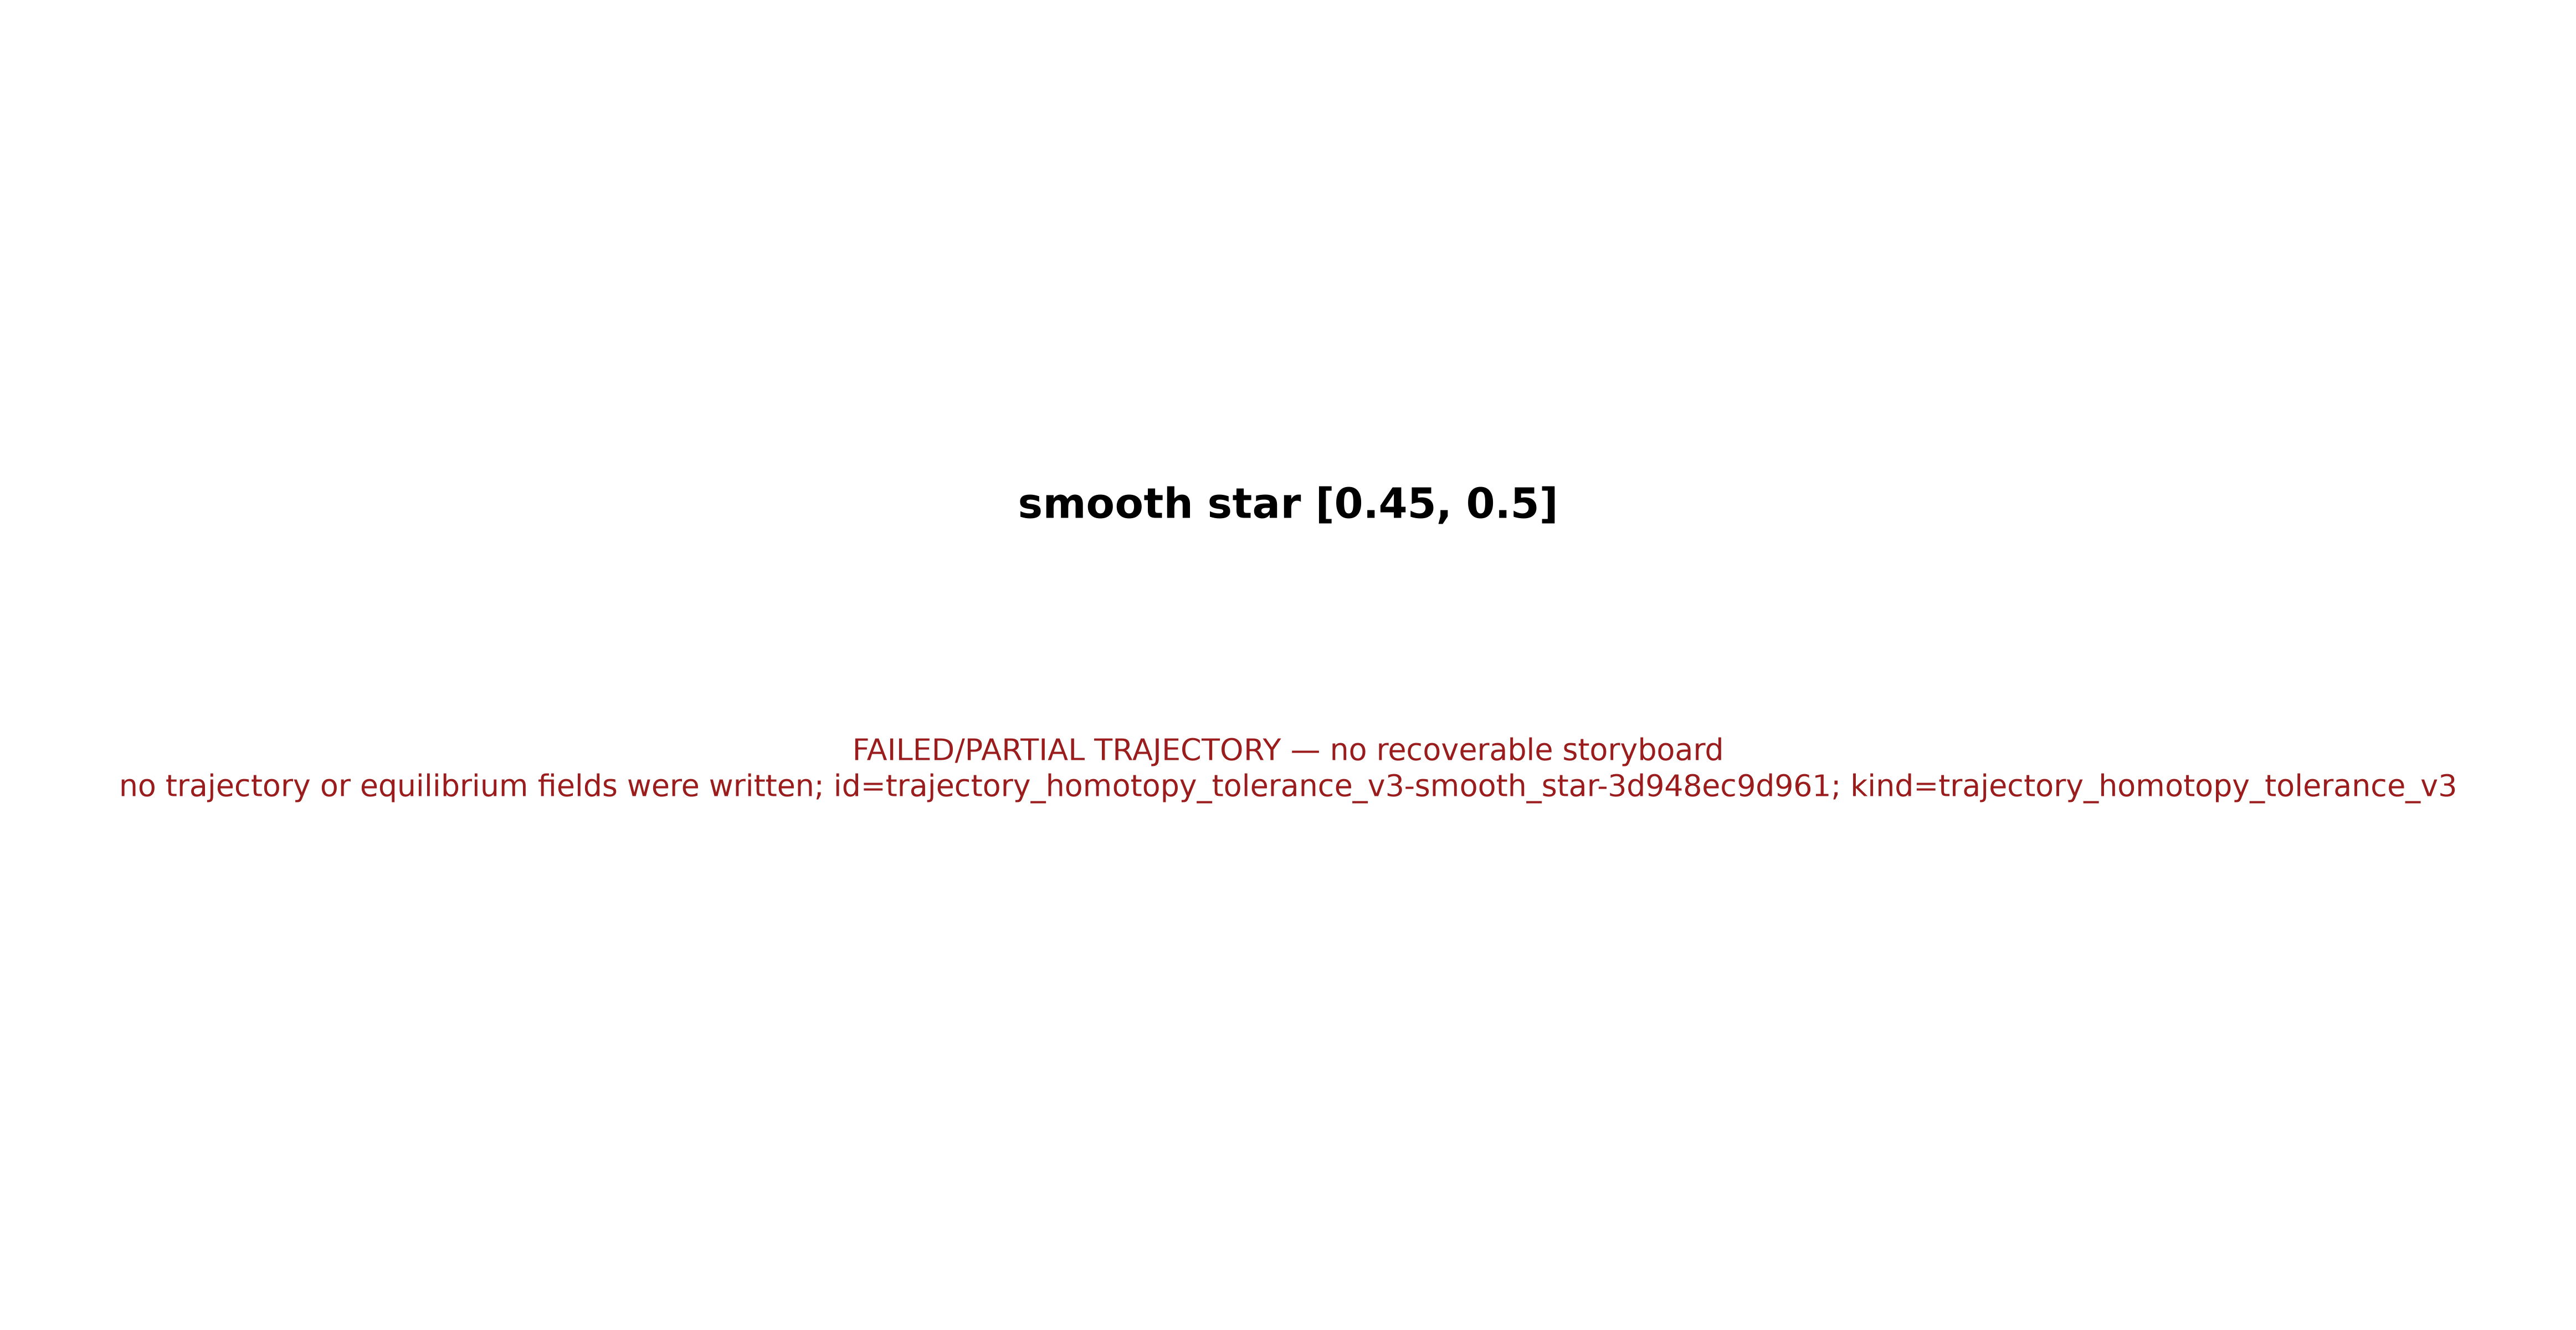
\includegraphics[width=0.88\linewidth]{figures/failed_band_evolution_001_smooth_star_0p45_0p5_trajectory_homotopy_tolerance_v3-smooth_star-3d948ec9d961.png}
\caption{Supplemental failed/partial trajectory evidence for smooth star at torsion levels $[0.45,0.5]$ (case trajectory\_homotopy\_tolerance\_v3-smooth\_star-3d948ec9d961; state=planned; classification=incomplete). The case is retained regardless of PDE or geometric success. Orange dashed curves are the fixed target band and blue solid curves are the moving equilibrium band; when state recovery is impossible, the PNG records the reason. Data status: diagnostic\_only.}
\label{fig:failed-storyboard-trajectory-homotopy-tolerance-v3-smooth-star-3d948ec9d961}
\end{figure}

\begin{figure}[tbp]
\centering
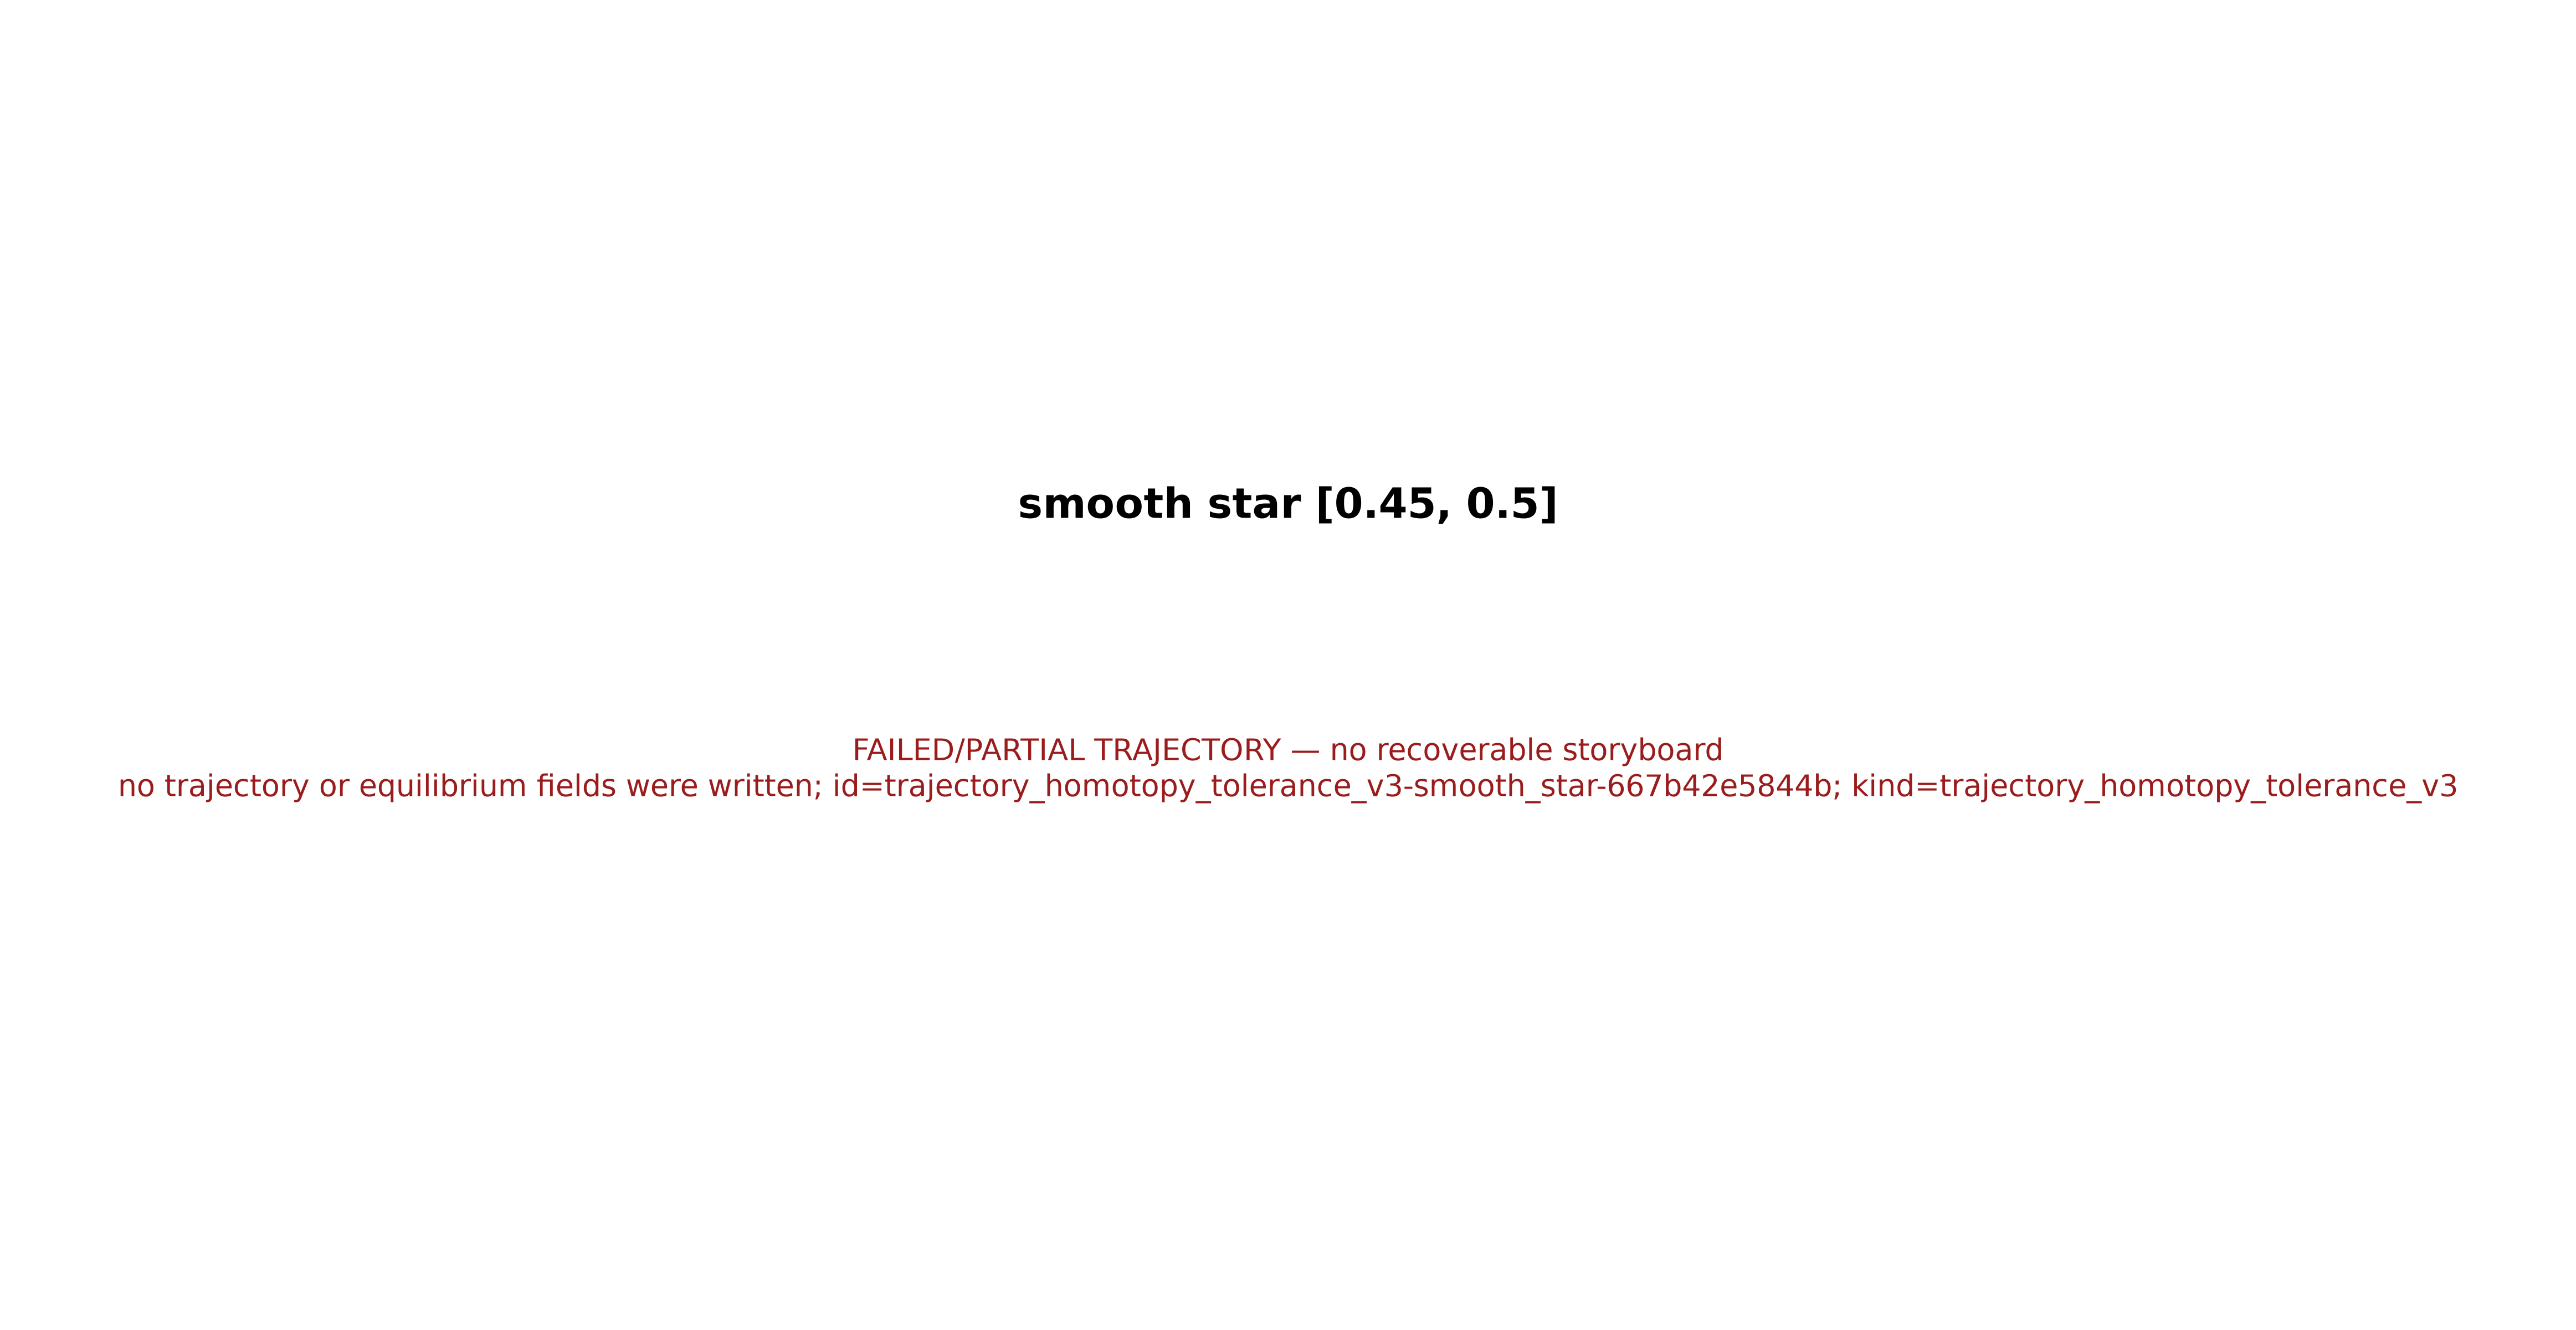
\includegraphics[width=0.88\linewidth]{figures/failed_band_evolution_002_smooth_star_0p45_0p5_trajectory_homotopy_tolerance_v3-smooth_star-667b42e5844b.png}
\caption{Supplemental failed/partial trajectory evidence for smooth star at torsion levels $[0.45,0.5]$ (case trajectory\_homotopy\_tolerance\_v3-smooth\_star-667b42e5844b; state=planned; classification=incomplete). The case is retained regardless of PDE or geometric success. Orange dashed curves are the fixed target band and blue solid curves are the moving equilibrium band; when state recovery is impossible, the PNG records the reason. Data status: diagnostic\_only.}
\label{fig:failed-storyboard-trajectory-homotopy-tolerance-v3-smooth-star-667b42e5844b}
\end{figure}

\begin{figure}[tbp]
\centering
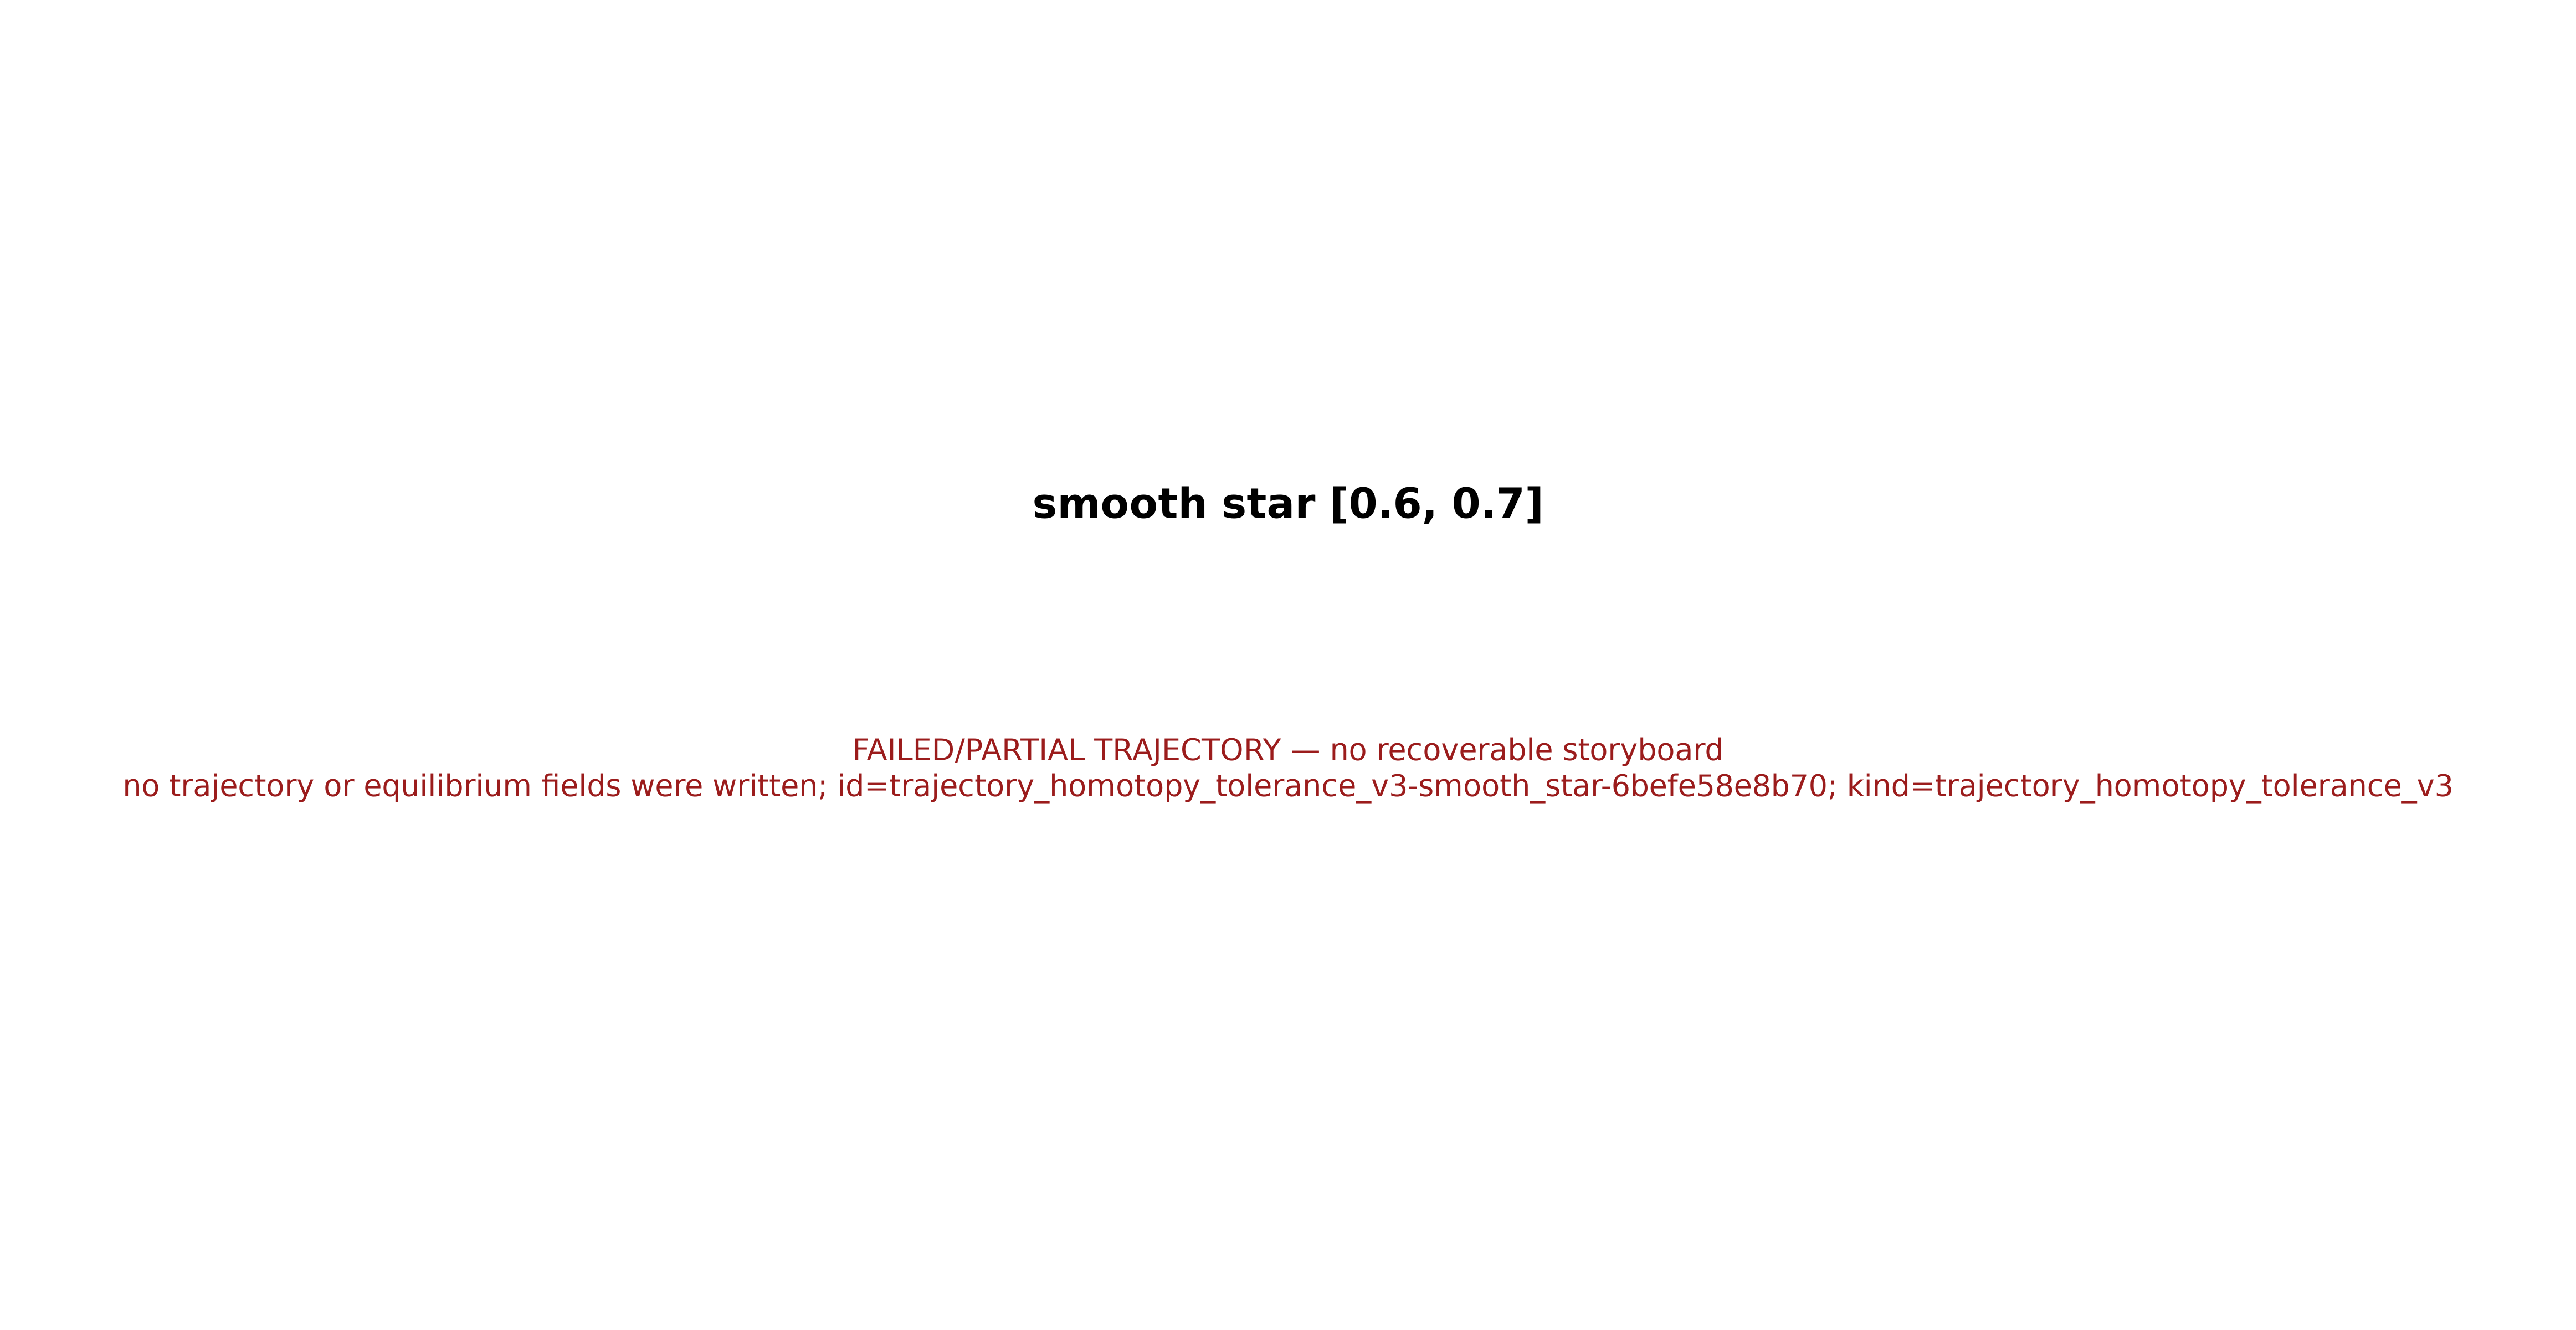
\includegraphics[width=0.88\linewidth]{figures/failed_band_evolution_003_smooth_star_0p6_0p7_trajectory_homotopy_tolerance_v3-smooth_star-6befe58e8b70.png}
\caption{Supplemental failed/partial trajectory evidence for smooth star at torsion levels $[0.6,0.7]$ (case trajectory\_homotopy\_tolerance\_v3-smooth\_star-6befe58e8b70; state=planned; classification=incomplete). The case is retained regardless of PDE or geometric success. Orange dashed curves are the fixed target band and blue solid curves are the moving equilibrium band; when state recovery is impossible, the PNG records the reason. Data status: diagnostic\_only.}
\label{fig:failed-storyboard-trajectory-homotopy-tolerance-v3-smooth-star-6befe58e8b70}
\end{figure}

\begin{figure}[tbp]
\centering
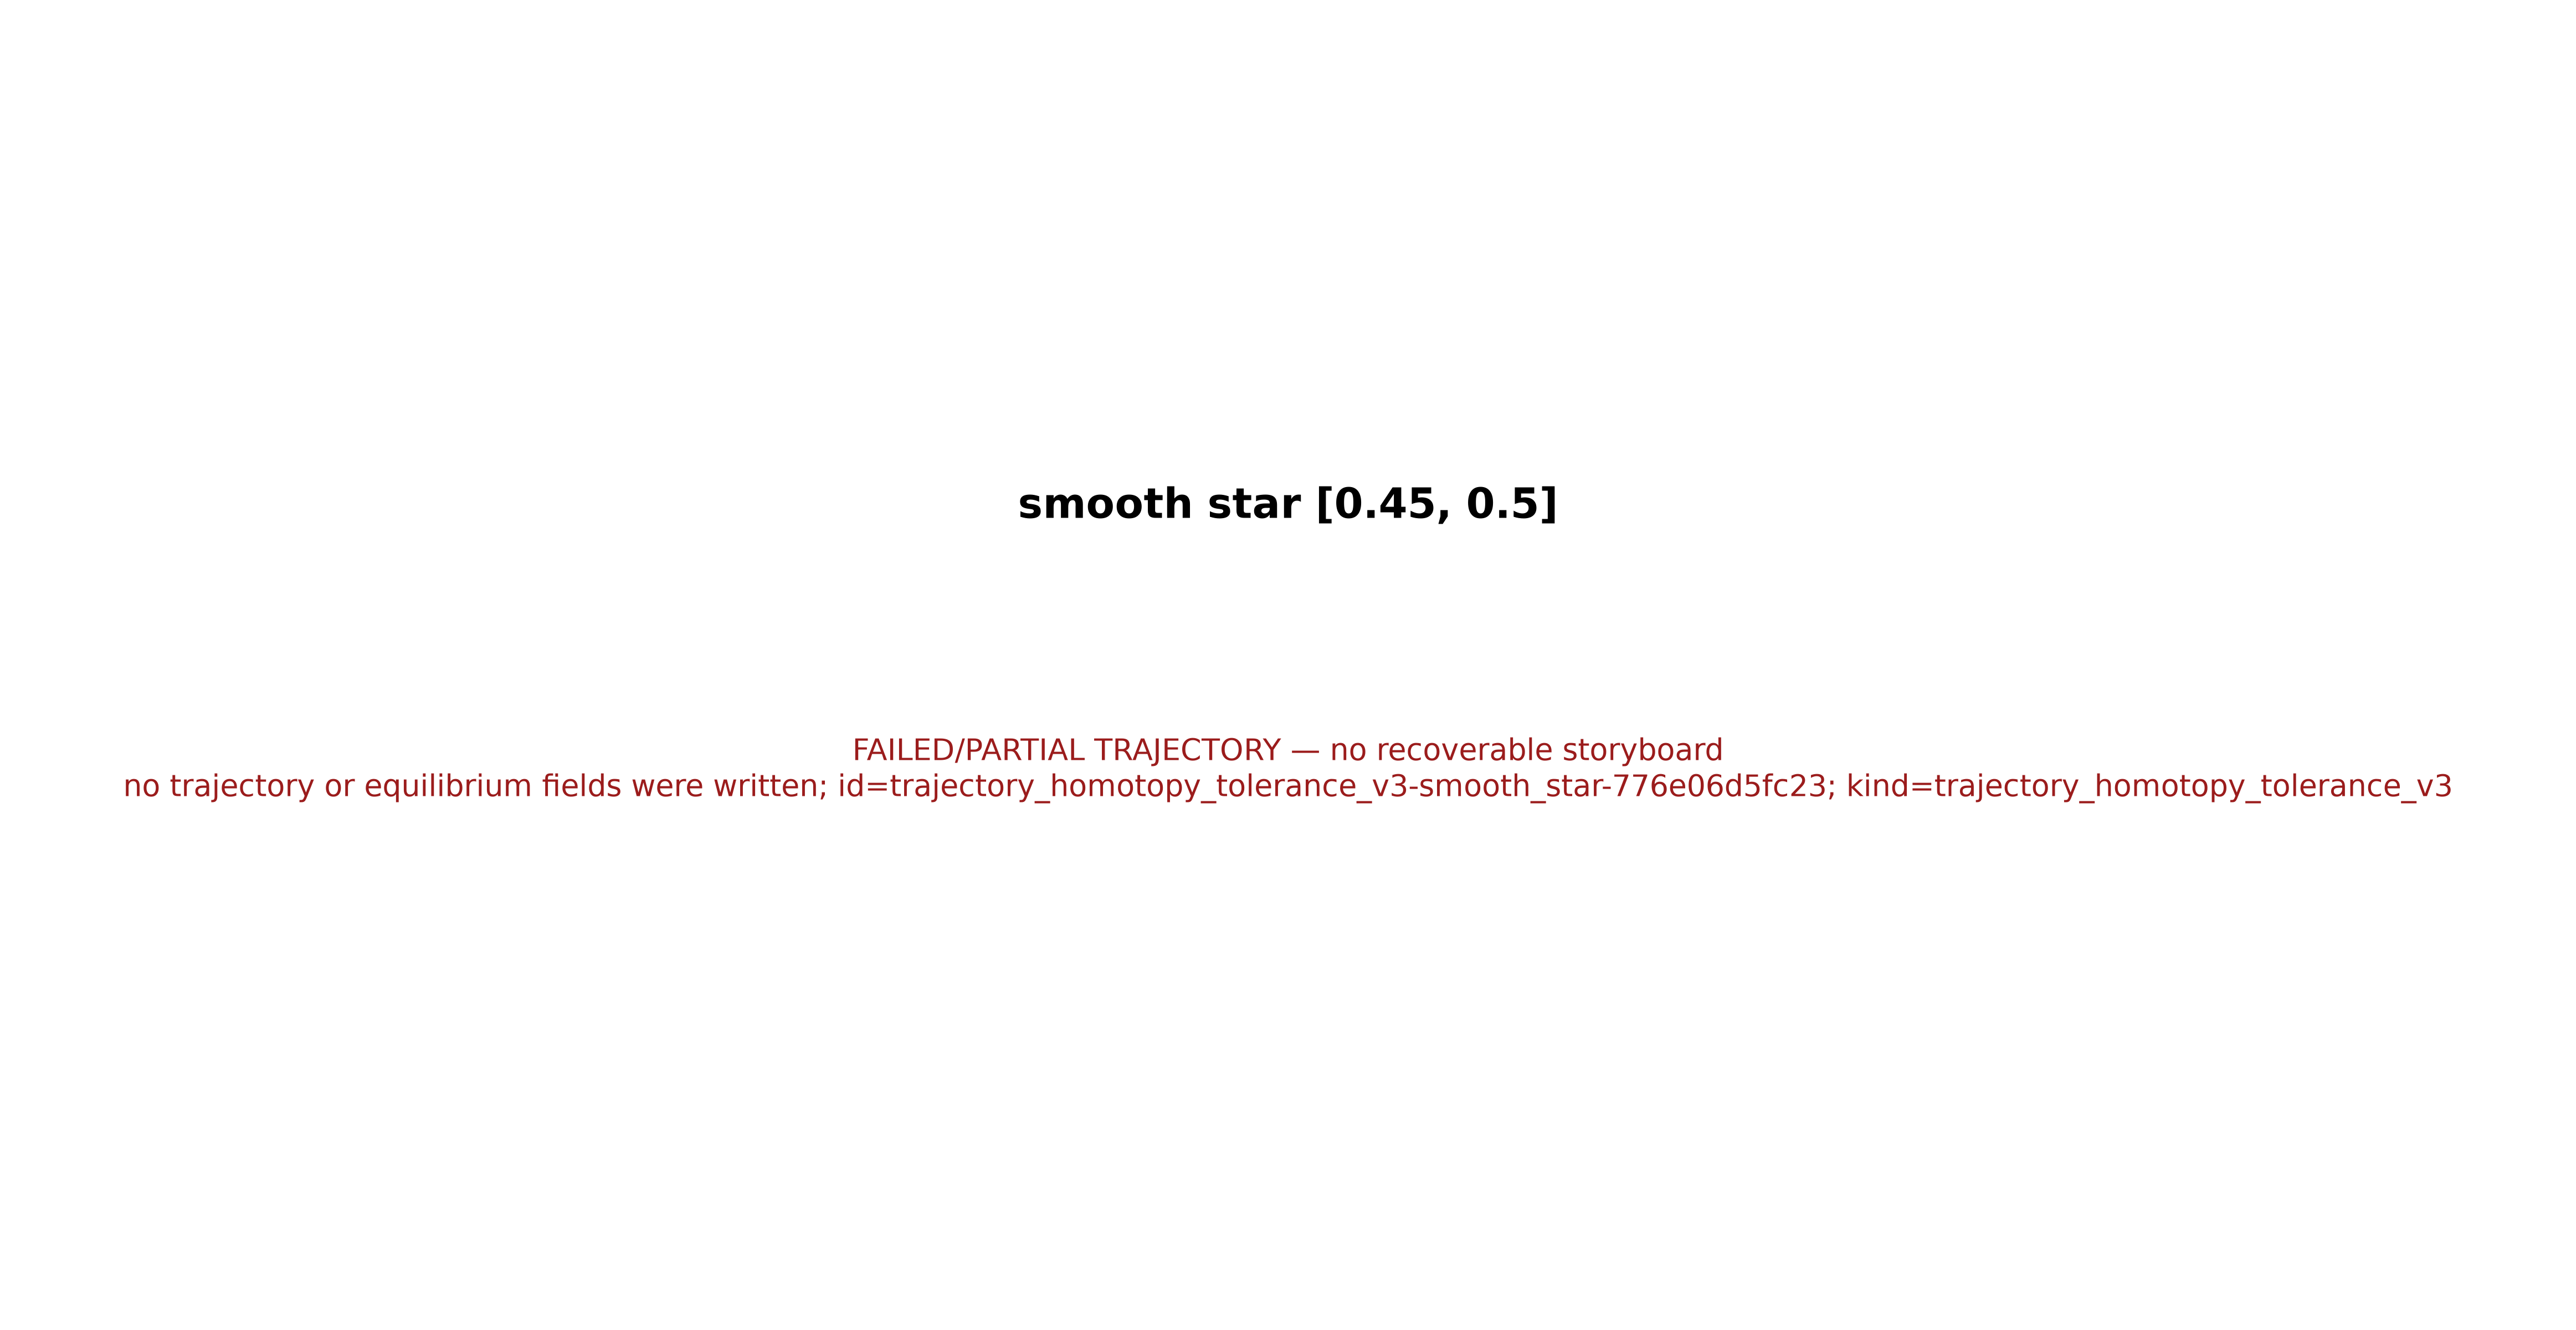
\includegraphics[width=0.88\linewidth]{figures/failed_band_evolution_004_smooth_star_0p45_0p5_trajectory_homotopy_tolerance_v3-smooth_star-776e06d5fc23.png}
\caption{Supplemental failed/partial trajectory evidence for smooth star at torsion levels $[0.45,0.5]$ (case trajectory\_homotopy\_tolerance\_v3-smooth\_star-776e06d5fc23; state=planned; classification=incomplete). The case is retained regardless of PDE or geometric success. Orange dashed curves are the fixed target band and blue solid curves are the moving equilibrium band; when state recovery is impossible, the PNG records the reason. Data status: diagnostic\_only.}
\label{fig:failed-storyboard-trajectory-homotopy-tolerance-v3-smooth-star-776e06d5fc23}
\end{figure}

\begin{figure}[tbp]
\centering
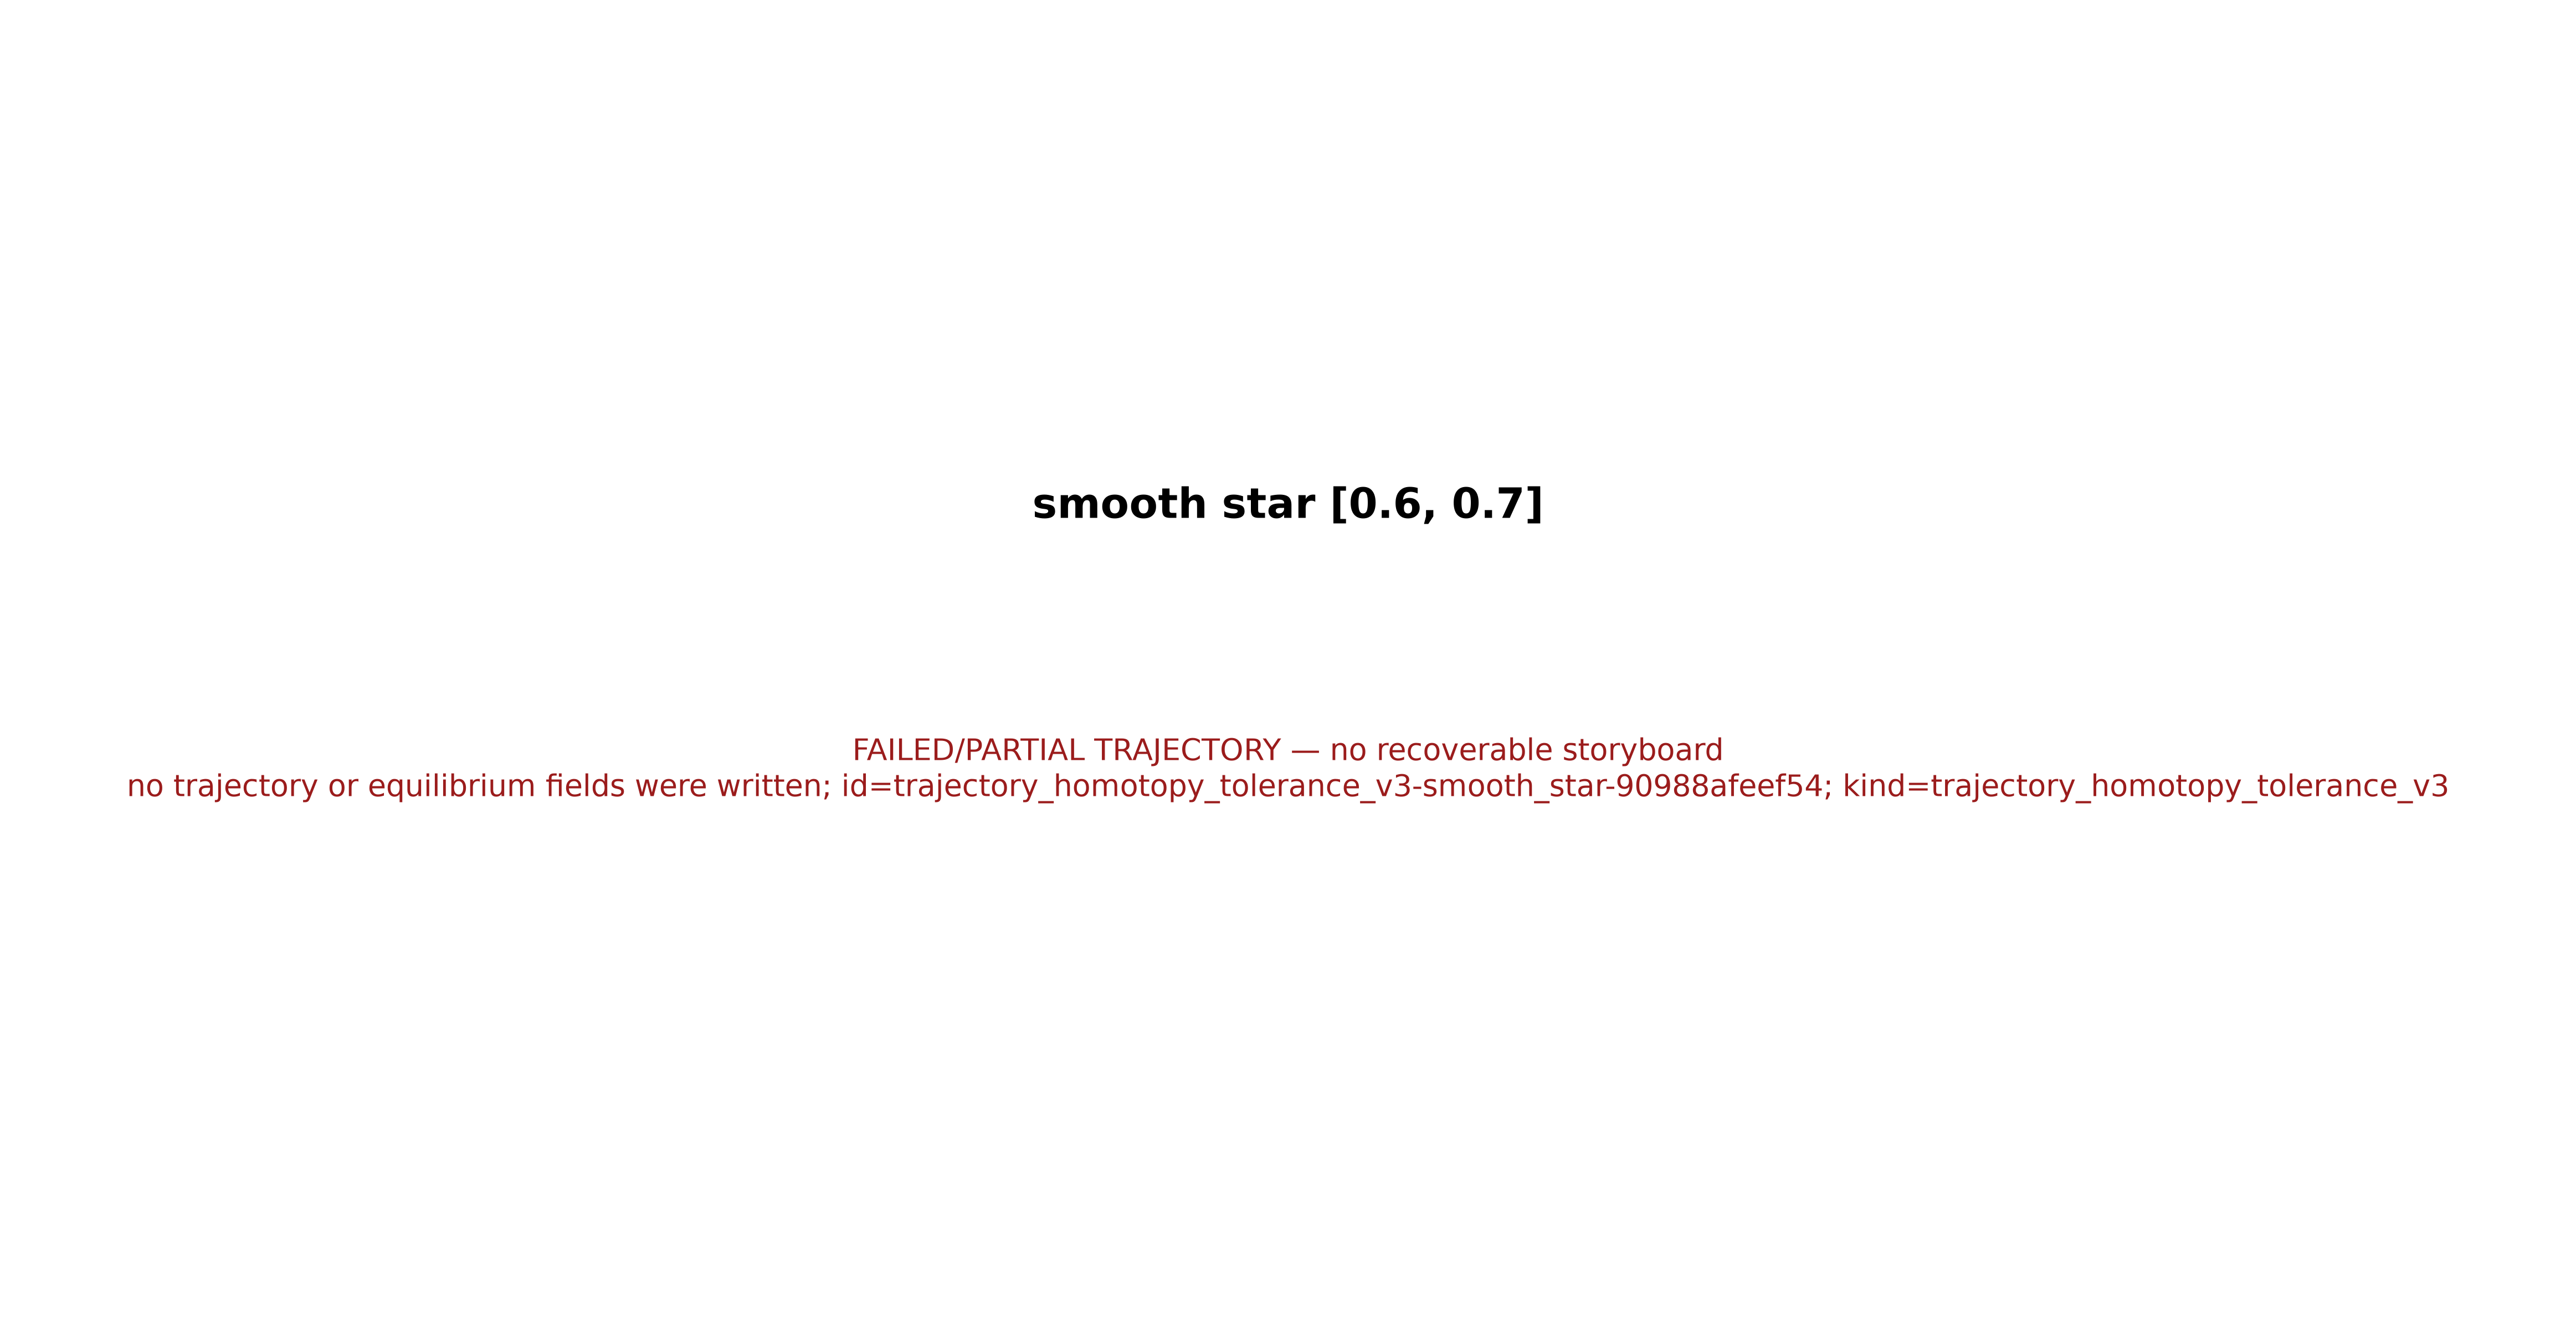
\includegraphics[width=0.88\linewidth]{figures/failed_band_evolution_005_smooth_star_0p6_0p7_trajectory_homotopy_tolerance_v3-smooth_star-90988afeef54.png}
\caption{Supplemental failed/partial trajectory evidence for smooth star at torsion levels $[0.6,0.7]$ (case trajectory\_homotopy\_tolerance\_v3-smooth\_star-90988afeef54; state=planned; classification=incomplete). The case is retained regardless of PDE or geometric success. Orange dashed curves are the fixed target band and blue solid curves are the moving equilibrium band; when state recovery is impossible, the PNG records the reason. Data status: diagnostic\_only.}
\label{fig:failed-storyboard-trajectory-homotopy-tolerance-v3-smooth-star-90988afeef54}
\end{figure}

\clearpage

\begin{figure}[tbp]
\centering
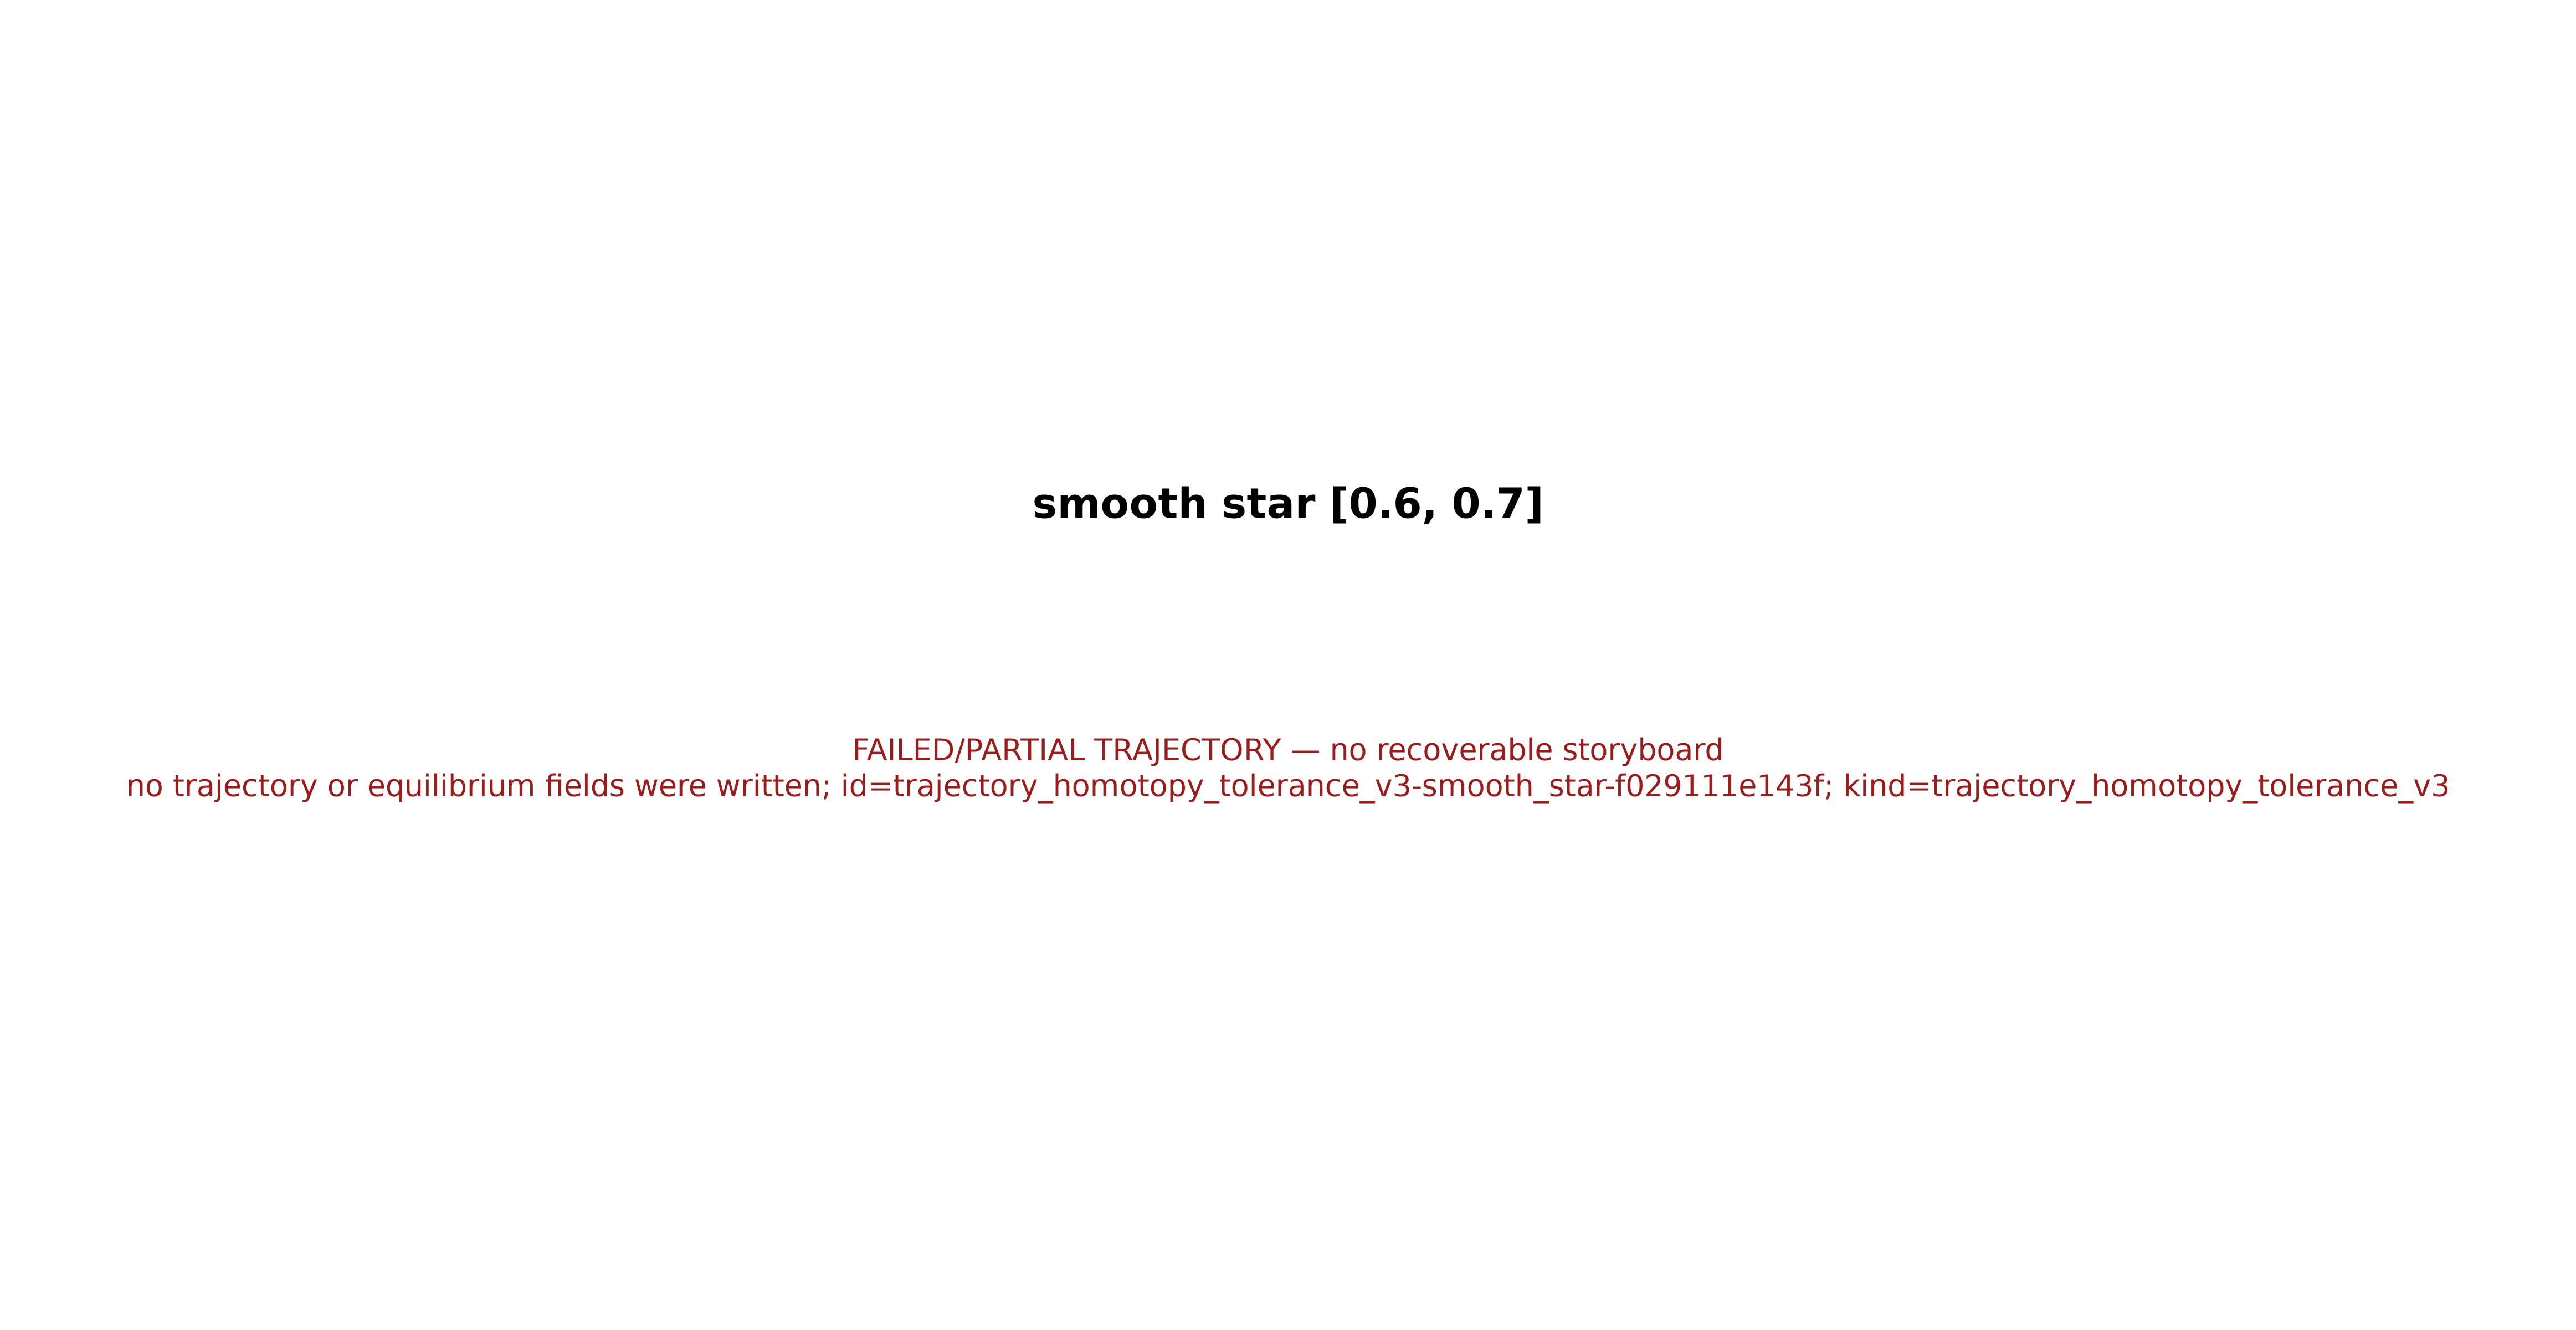
\includegraphics[width=0.88\linewidth]{figures/failed_band_evolution_006_smooth_star_0p6_0p7_trajectory_homotopy_tolerance_v3-smooth_star-f029111e143f.png}
\caption{Supplemental failed/partial trajectory evidence for smooth star at torsion levels $[0.6,0.7]$ (case trajectory\_homotopy\_tolerance\_v3-smooth\_star-f029111e143f; state=planned; classification=incomplete). The case is retained regardless of PDE or geometric success. Orange dashed curves are the fixed target band and blue solid curves are the moving equilibrium band; when state recovery is impossible, the PNG records the reason. Data status: diagnostic\_only.}
\label{fig:failed-storyboard-trajectory-homotopy-tolerance-v3-smooth-star-f029111e143f}
\end{figure}

\begin{figure}[tbp]
\centering
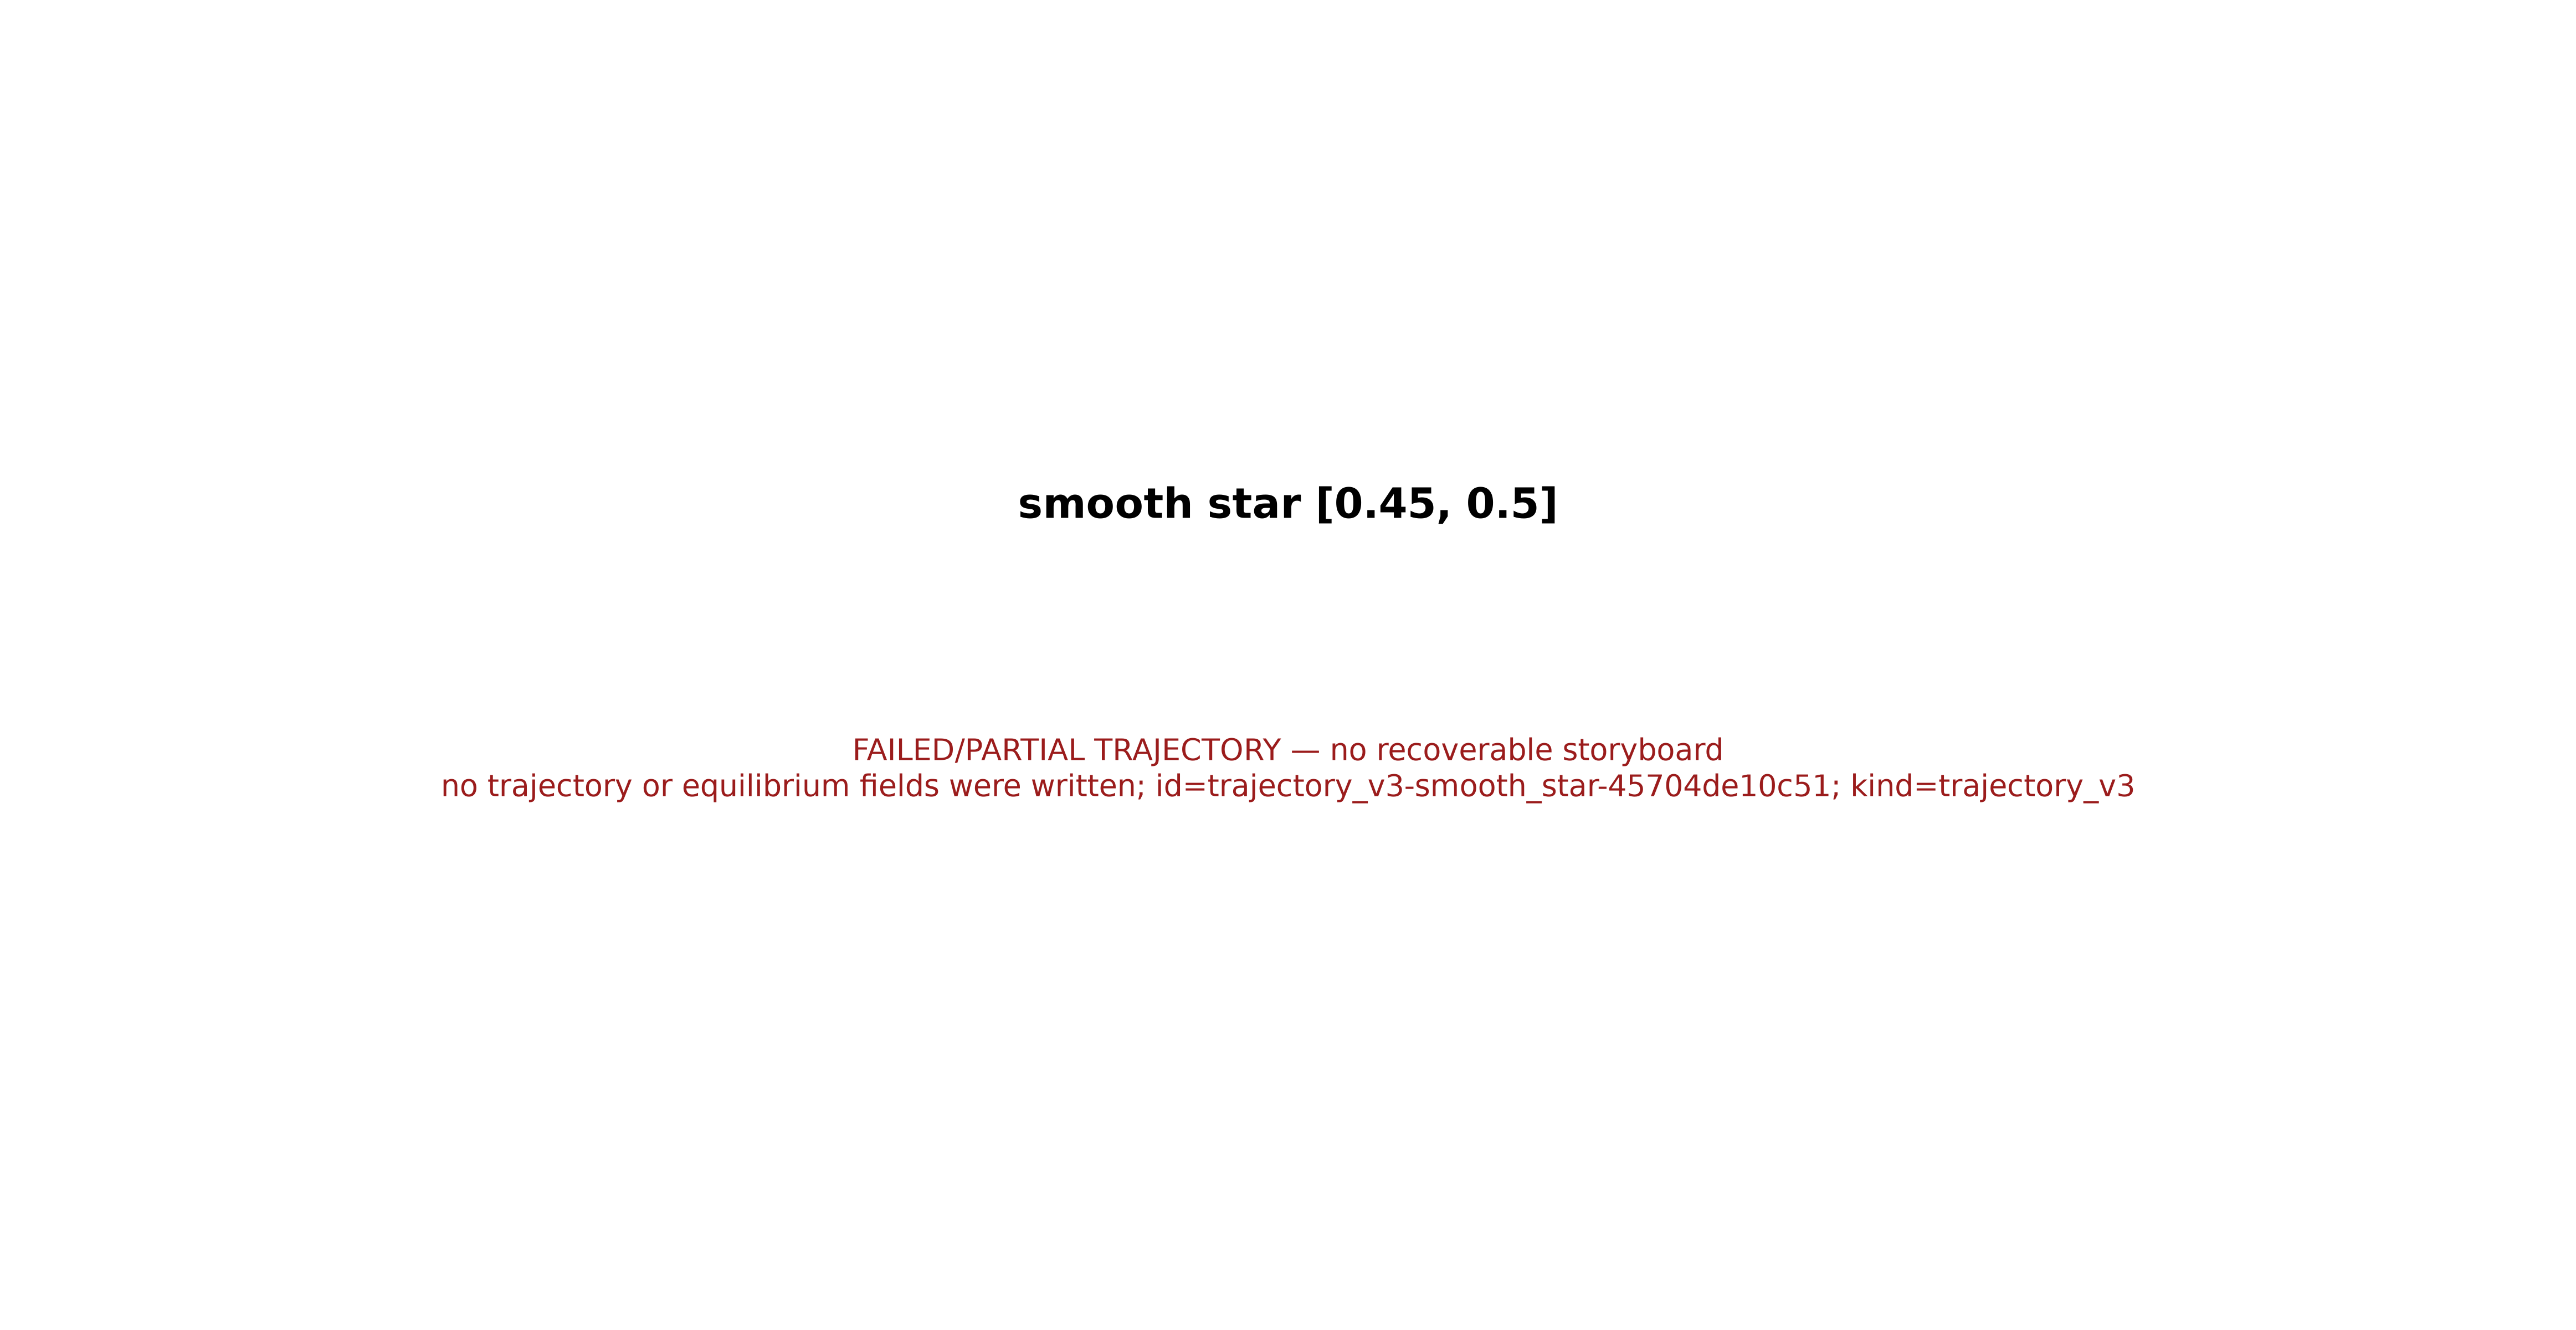
\includegraphics[width=0.88\linewidth]{figures/failed_band_evolution_007_smooth_star_0p45_0p5_trajectory_v3-smooth_star-45704de10c51.png}
\caption{Supplemental failed/partial trajectory evidence for smooth star at torsion levels $[0.45,0.5]$ (case trajectory\_v3-smooth\_star-45704de10c51; state=planned; classification=incomplete). The case is retained regardless of PDE or geometric success. Orange dashed curves are the fixed target band and blue solid curves are the moving equilibrium band; when state recovery is impossible, the PNG records the reason. Data status: diagnostic\_only.}
\label{fig:failed-storyboard-trajectory-v3-smooth-star-45704de10c51}
\end{figure}

\begin{figure}[tbp]
\centering
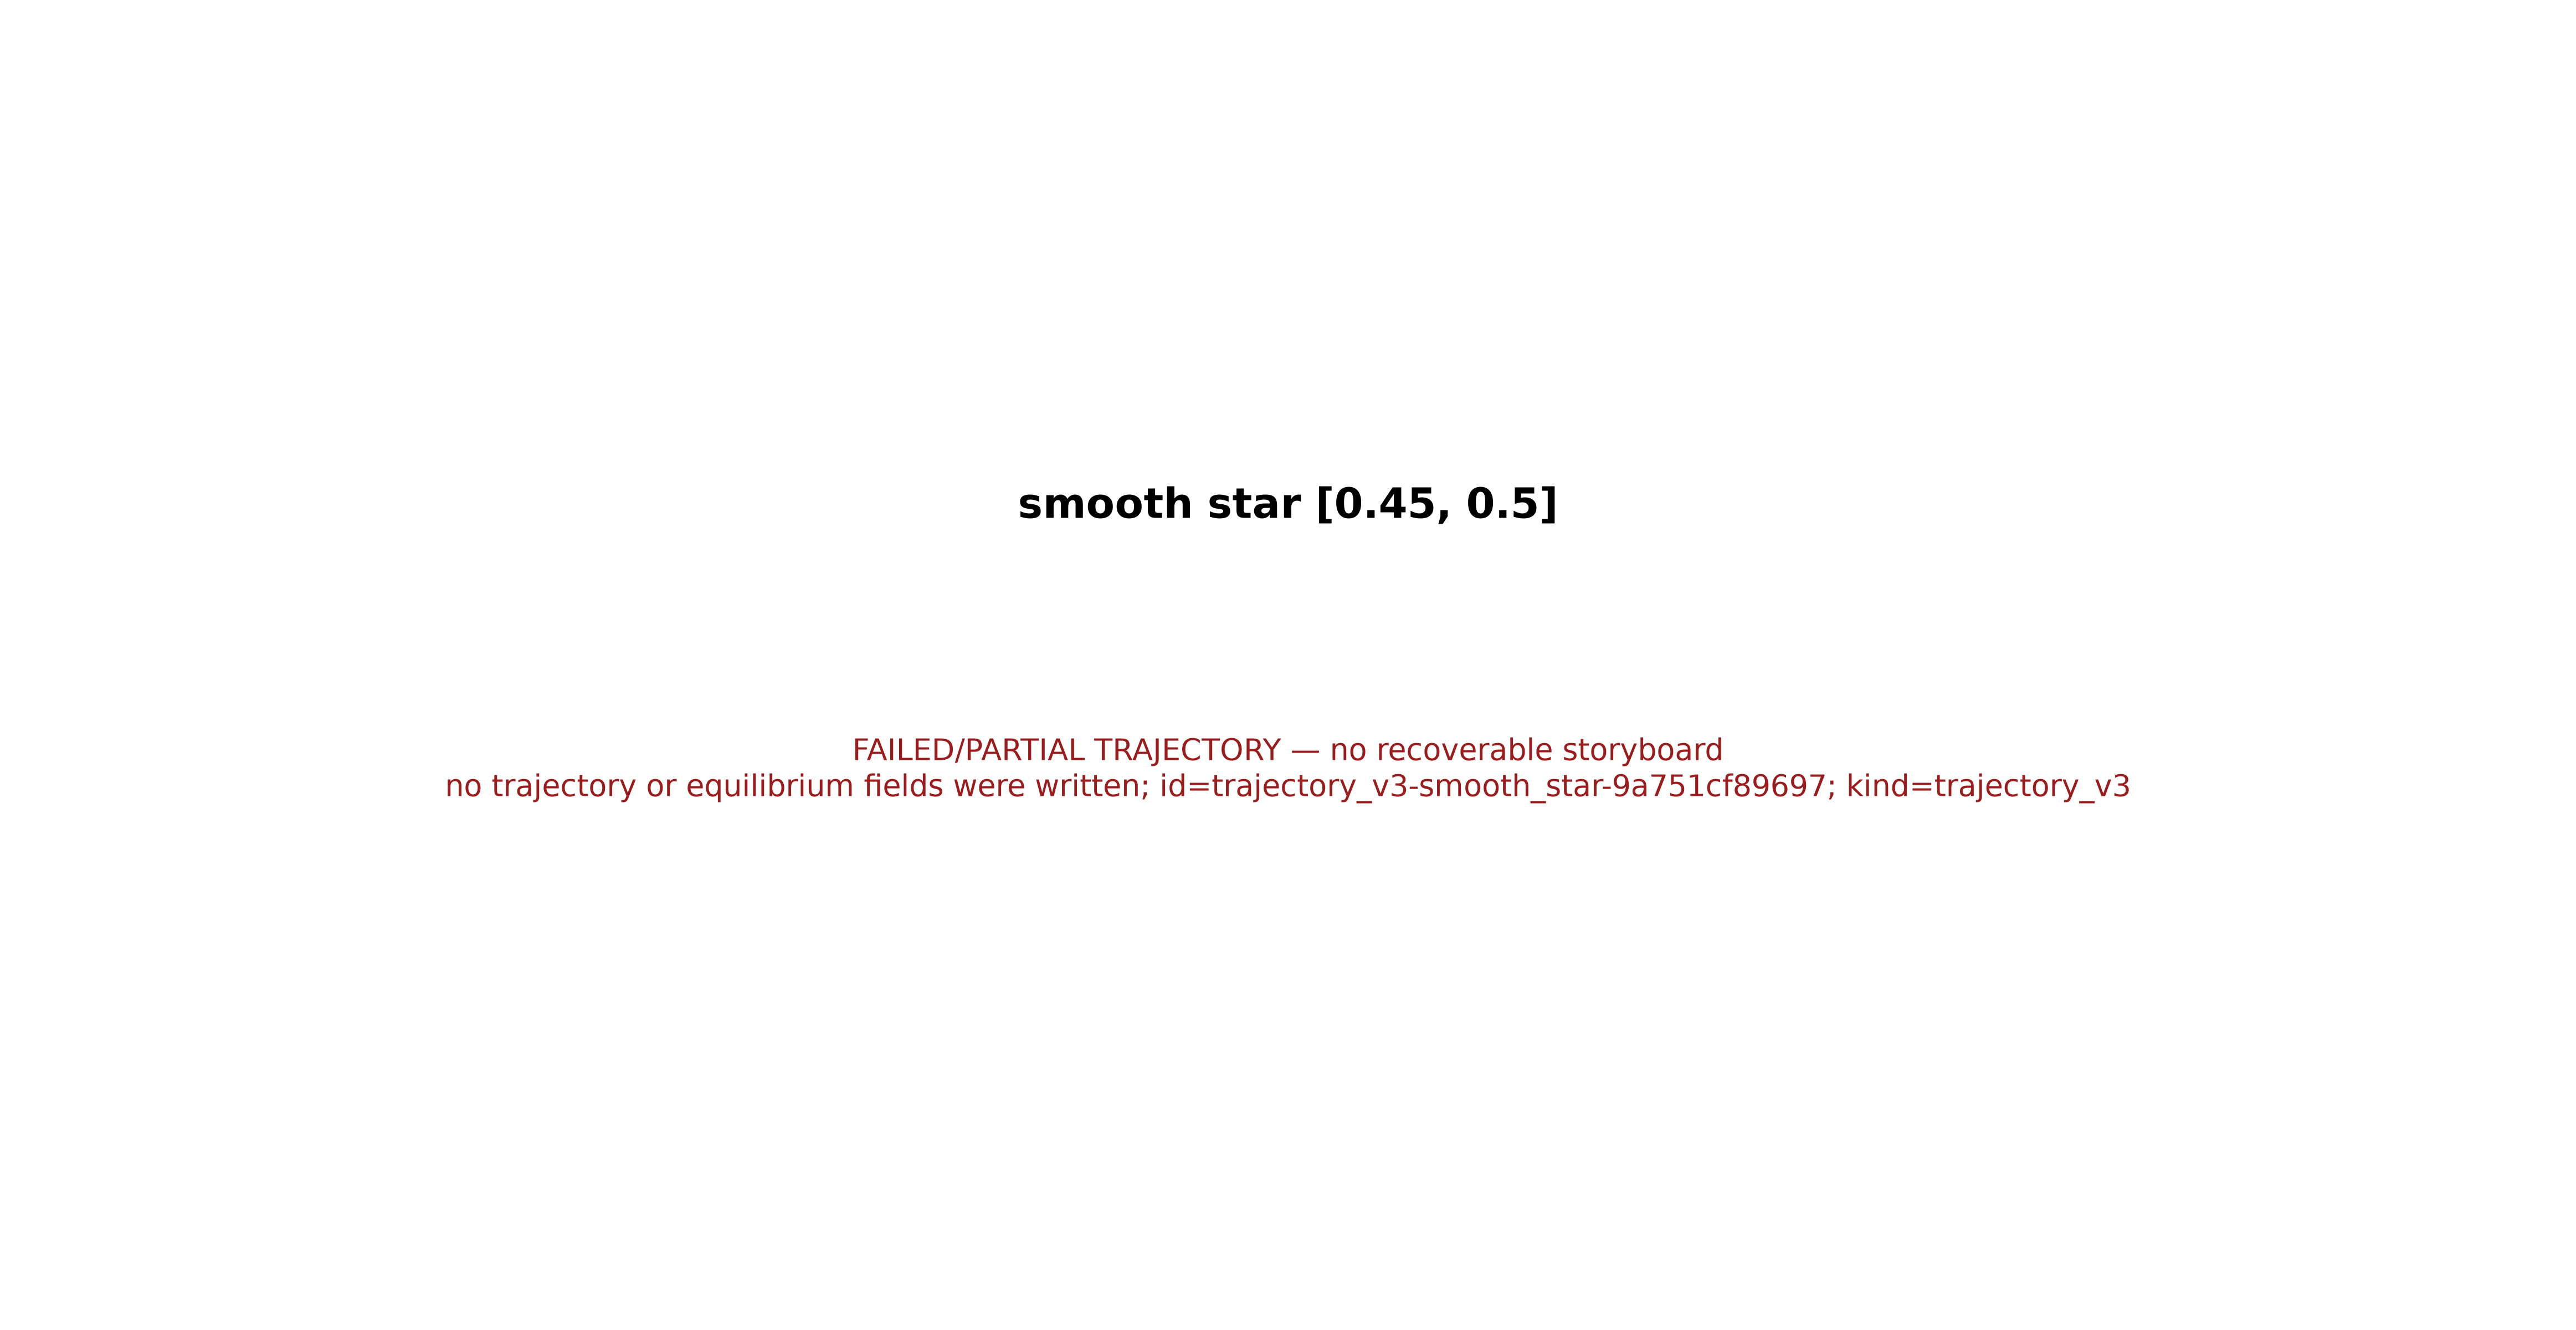
\includegraphics[width=0.88\linewidth]{figures/failed_band_evolution_008_smooth_star_0p45_0p5_trajectory_v3-smooth_star-9a751cf89697.png}
\caption{Supplemental failed/partial trajectory evidence for smooth star at torsion levels $[0.45,0.5]$ (case trajectory\_v3-smooth\_star-9a751cf89697; state=deferred; classification=deferred). The case is retained regardless of PDE or geometric success. Orange dashed curves are the fixed target band and blue solid curves are the moving equilibrium band; when state recovery is impossible, the PNG records the reason. Data status: diagnostic\_only.}
\label{fig:failed-storyboard-trajectory-v3-smooth-star-9a751cf89697}
\end{figure}

\begin{figure}[tbp]
\centering
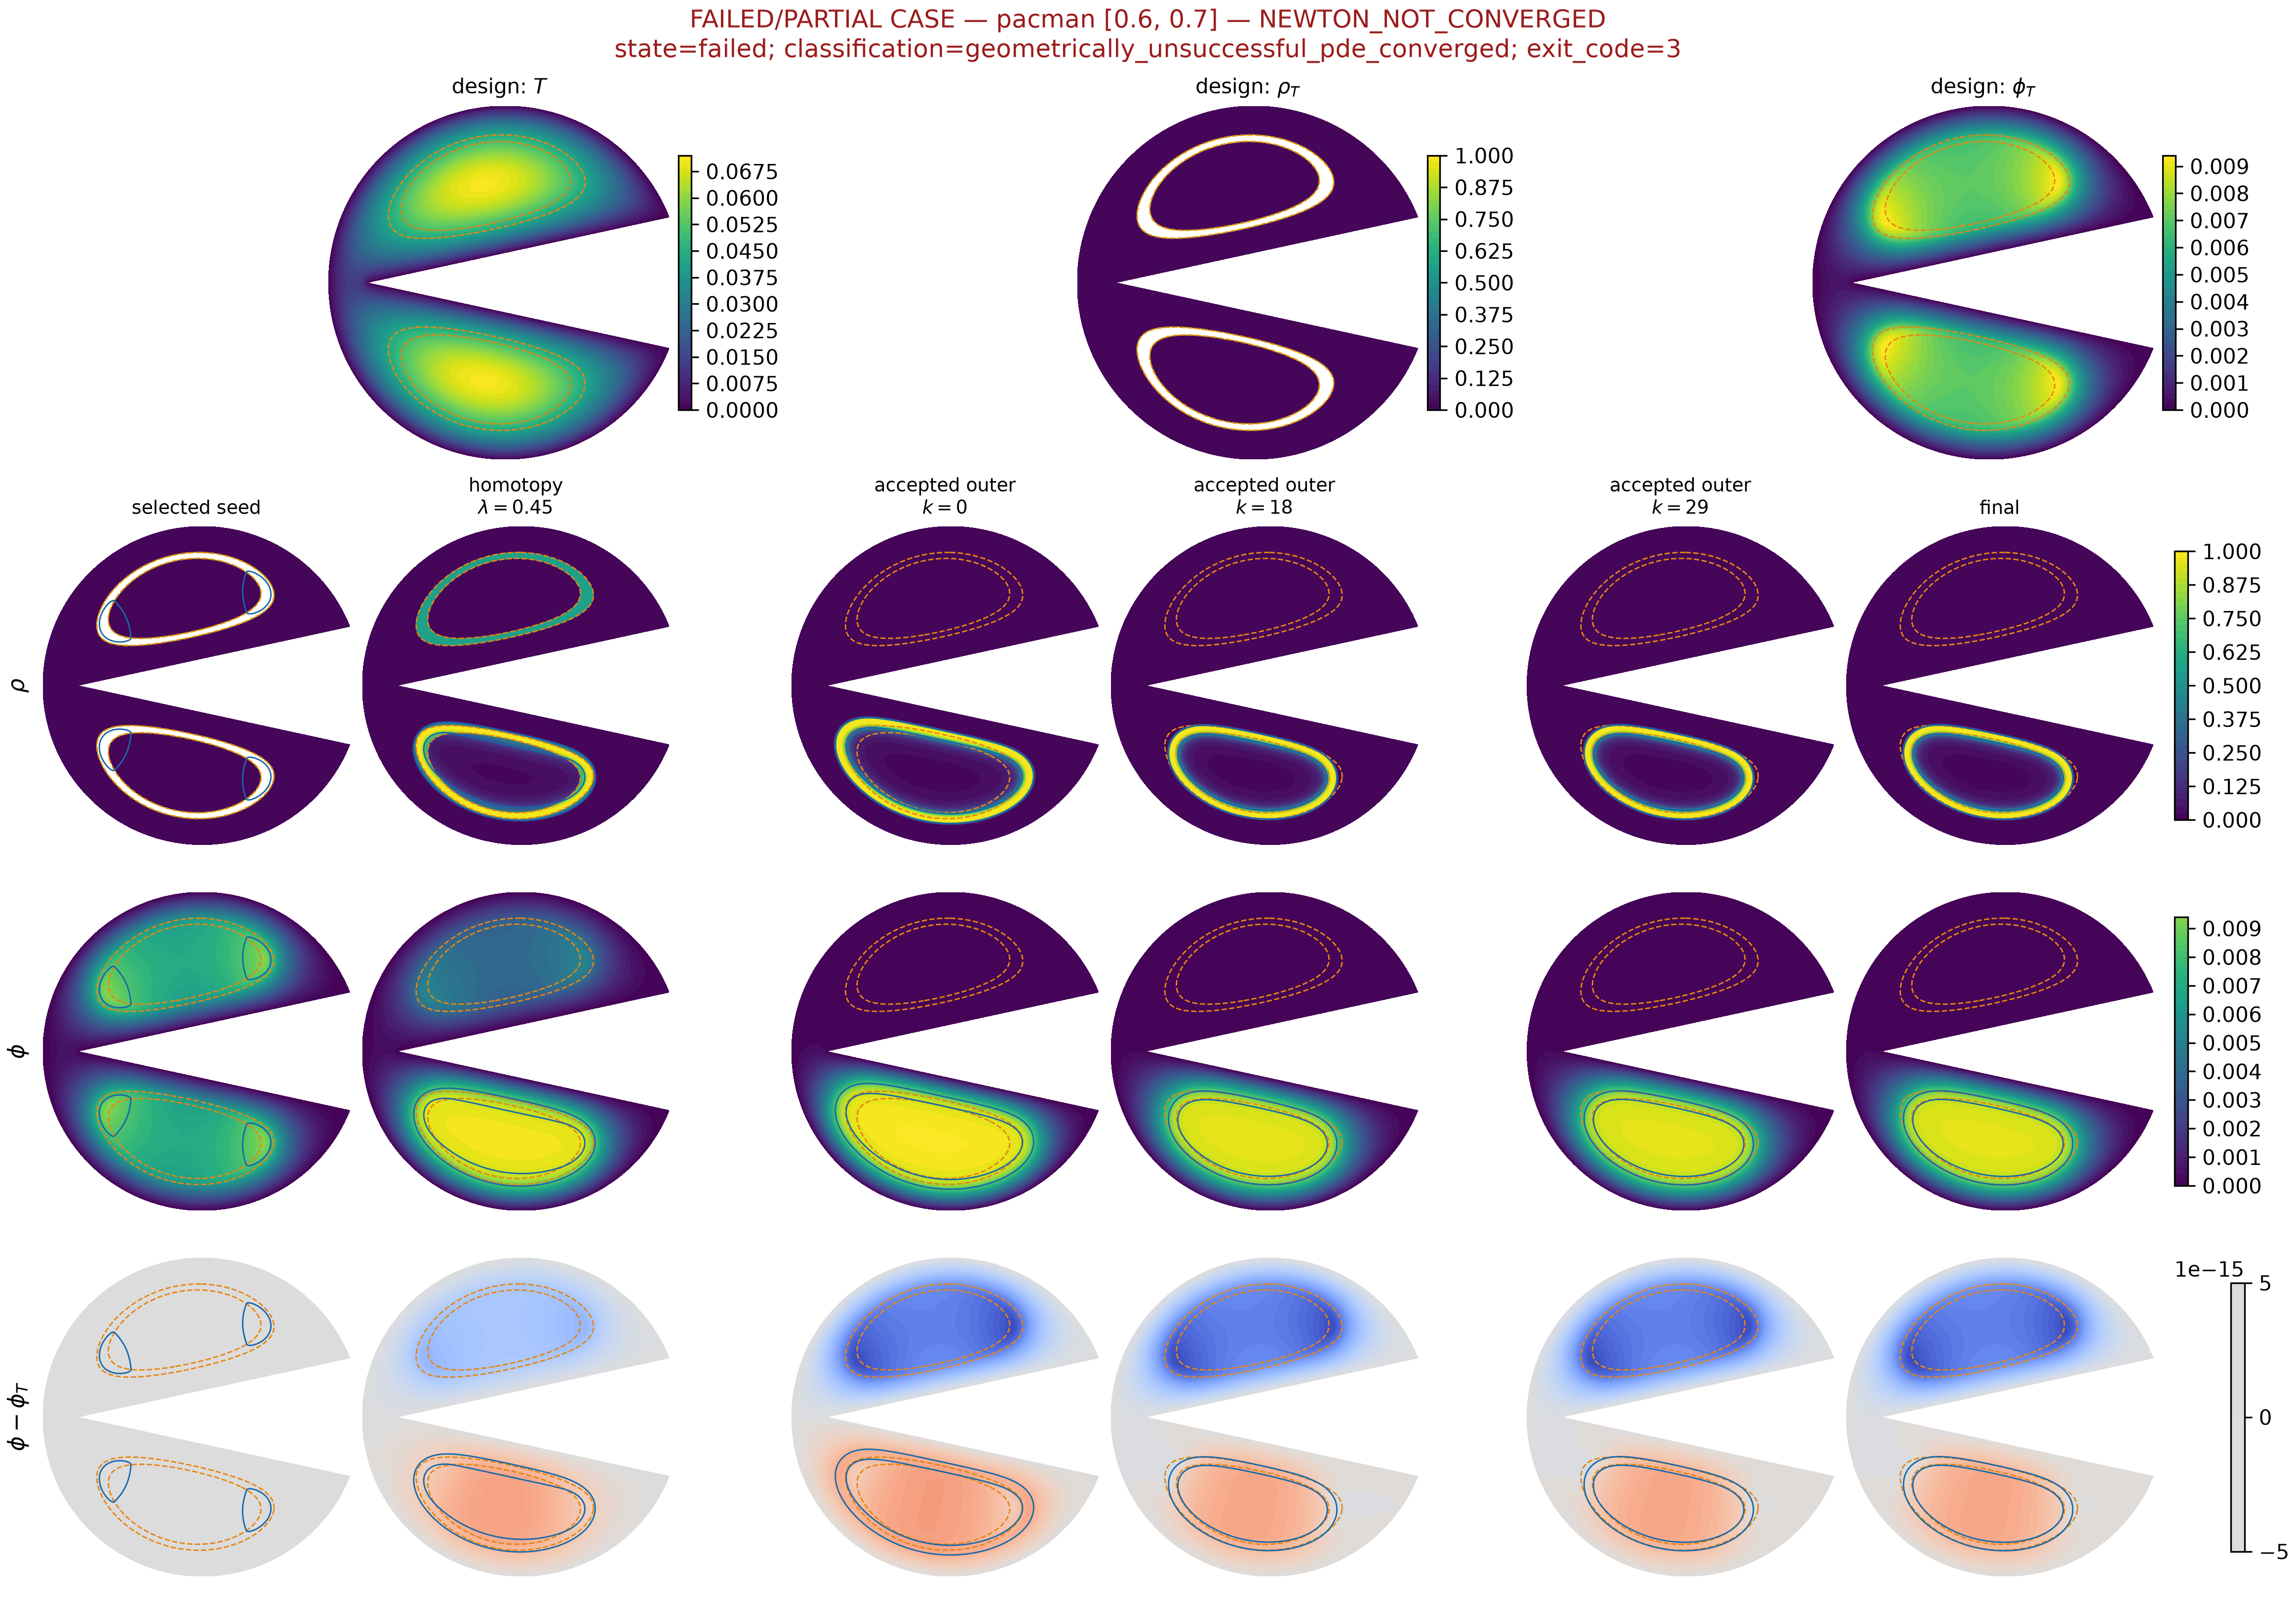
\includegraphics[width=0.88\linewidth]{figures/failed_band_evolution_009_pacman_0p6_0p7_trajectory-pacman-f64373773ee3.png}
\caption{Supplemental failed/partial trajectory evidence for pacman at torsion levels $[0.6,0.7]$ (case trajectory-pacman-f64373773ee3; state=failed; classification=geometrically\_unsuccessful\_pde\_converged). The case is retained regardless of PDE or geometric success. Orange dashed curves are the fixed target band and blue solid curves are the moving equilibrium band; when state recovery is impossible, the PNG records the reason. Data status: actual.}
\label{fig:failed-storyboard-trajectory-pacman-f64373773ee3}
\end{figure}

\begin{figure}[tbp]
\centering
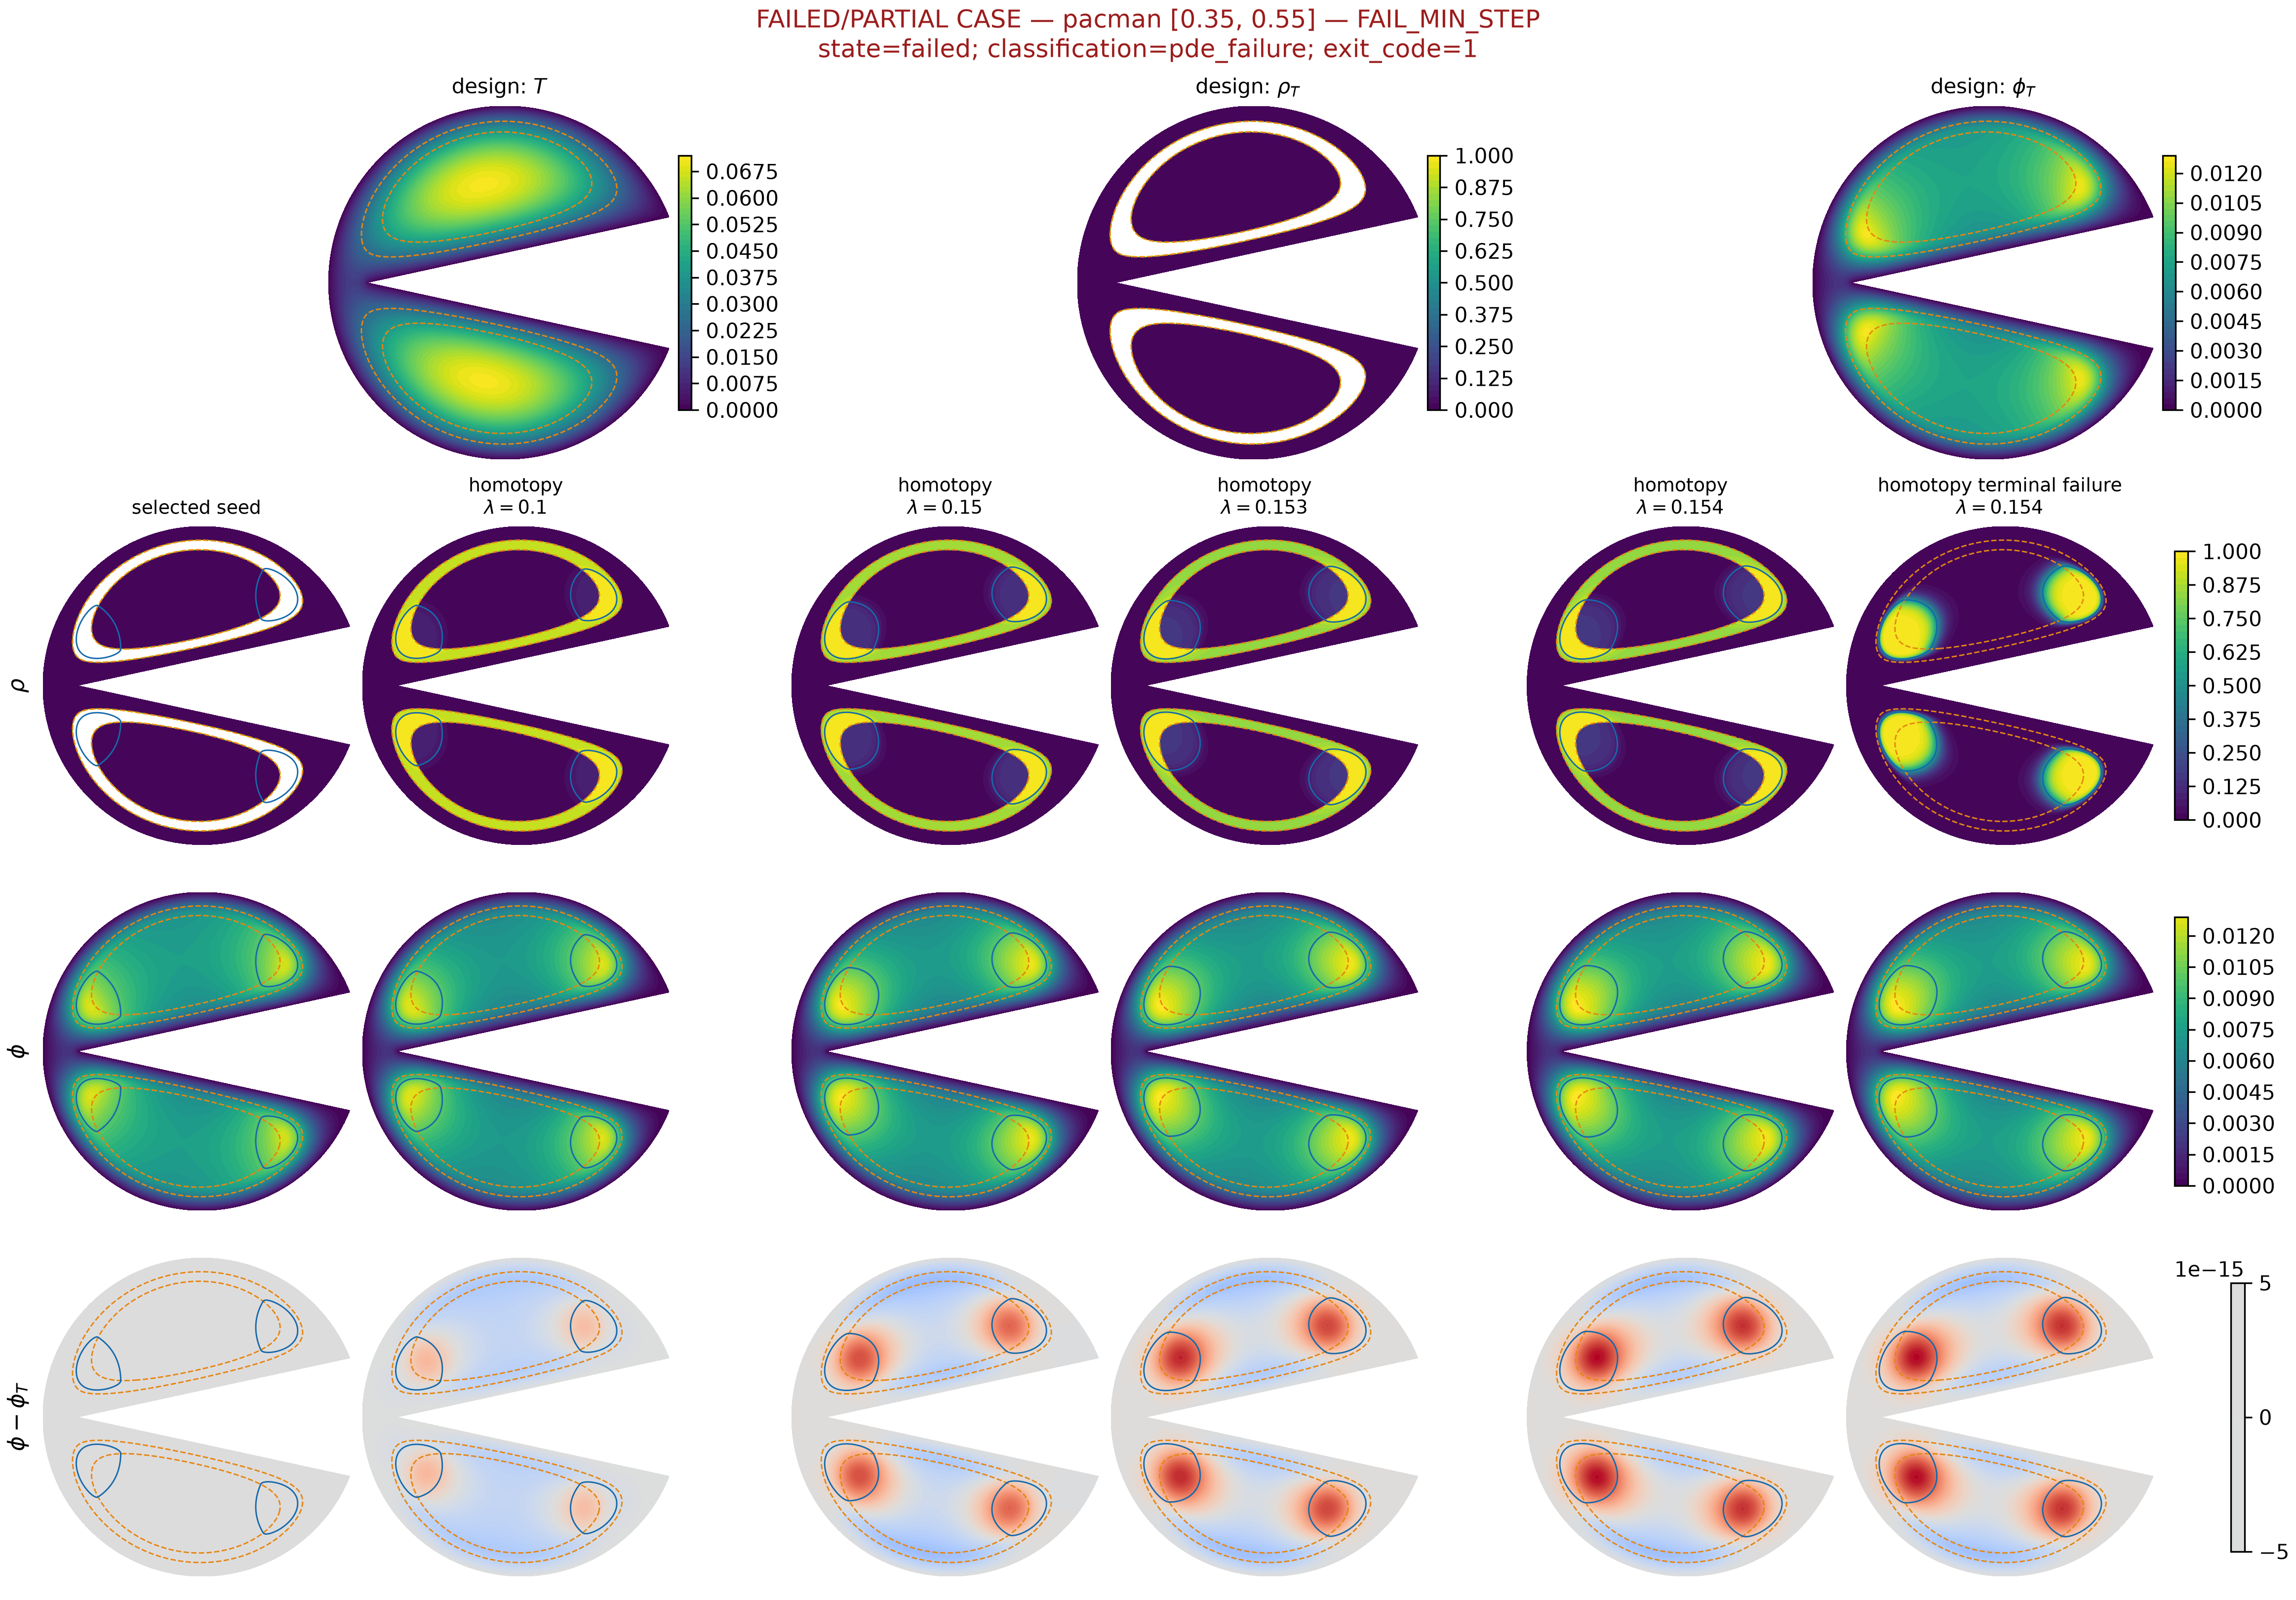
\includegraphics[width=0.88\linewidth]{figures/failed_band_evolution_010_pacman_0p35_0p55_trajectory_candidate-pacman-2c721469f3bd.png}
\caption{Supplemental failed/partial trajectory evidence for pacman at torsion levels $[0.35,0.55]$ (case trajectory\_candidate-pacman-2c721469f3bd; state=failed; classification=pde\_failure). The case is retained regardless of PDE or geometric success. Orange dashed curves are the fixed target band and blue solid curves are the moving equilibrium band; when state recovery is impossible, the PNG records the reason. Data status: actual.}
\label{fig:failed-storyboard-trajectory-candidate-pacman-2c721469f3bd}
\end{figure}

\begin{figure}[tbp]
\centering
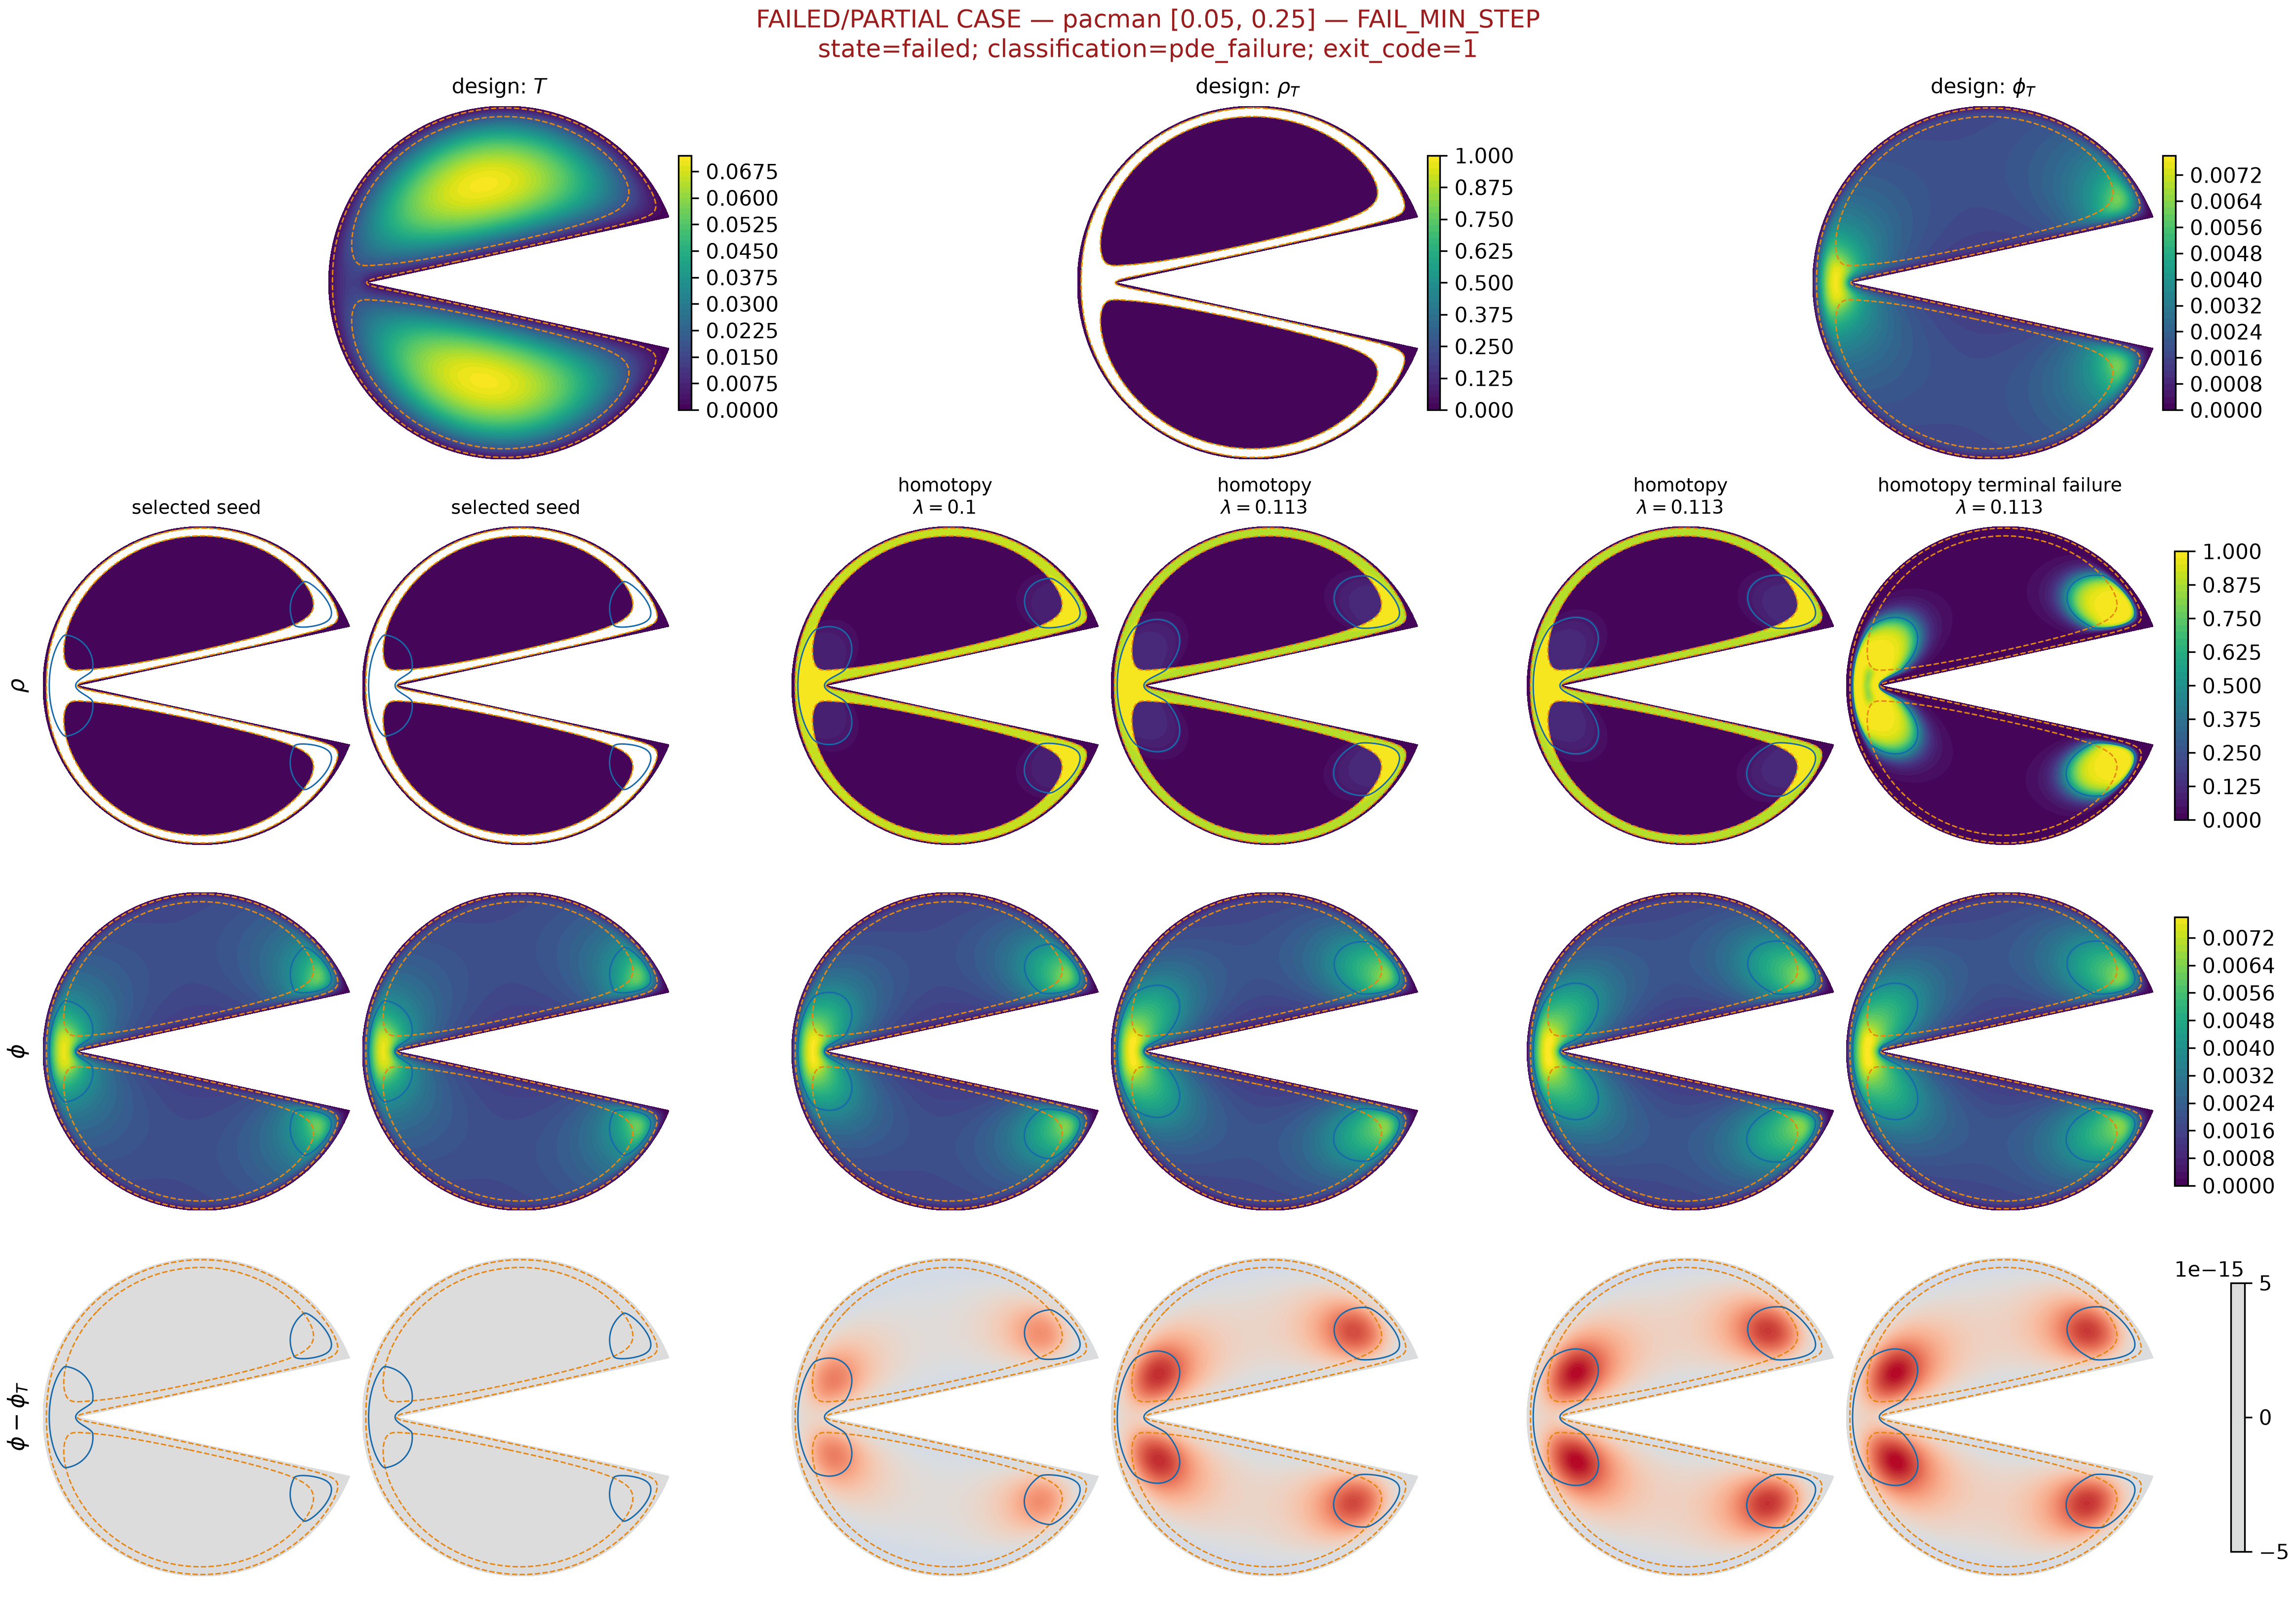
\includegraphics[width=0.88\linewidth]{figures/failed_band_evolution_011_pacman_0p05_0p25_trajectory_candidate-pacman-39c11e1119bf.png}
\caption{Supplemental failed/partial trajectory evidence for pacman at torsion levels $[0.05,0.25]$ (case trajectory\_candidate-pacman-39c11e1119bf; state=failed; classification=pde\_failure). The case is retained regardless of PDE or geometric success. Orange dashed curves are the fixed target band and blue solid curves are the moving equilibrium band; when state recovery is impossible, the PNG records the reason. Data status: actual.}
\label{fig:failed-storyboard-trajectory-candidate-pacman-39c11e1119bf}
\end{figure}

\begin{figure}[tbp]
\centering
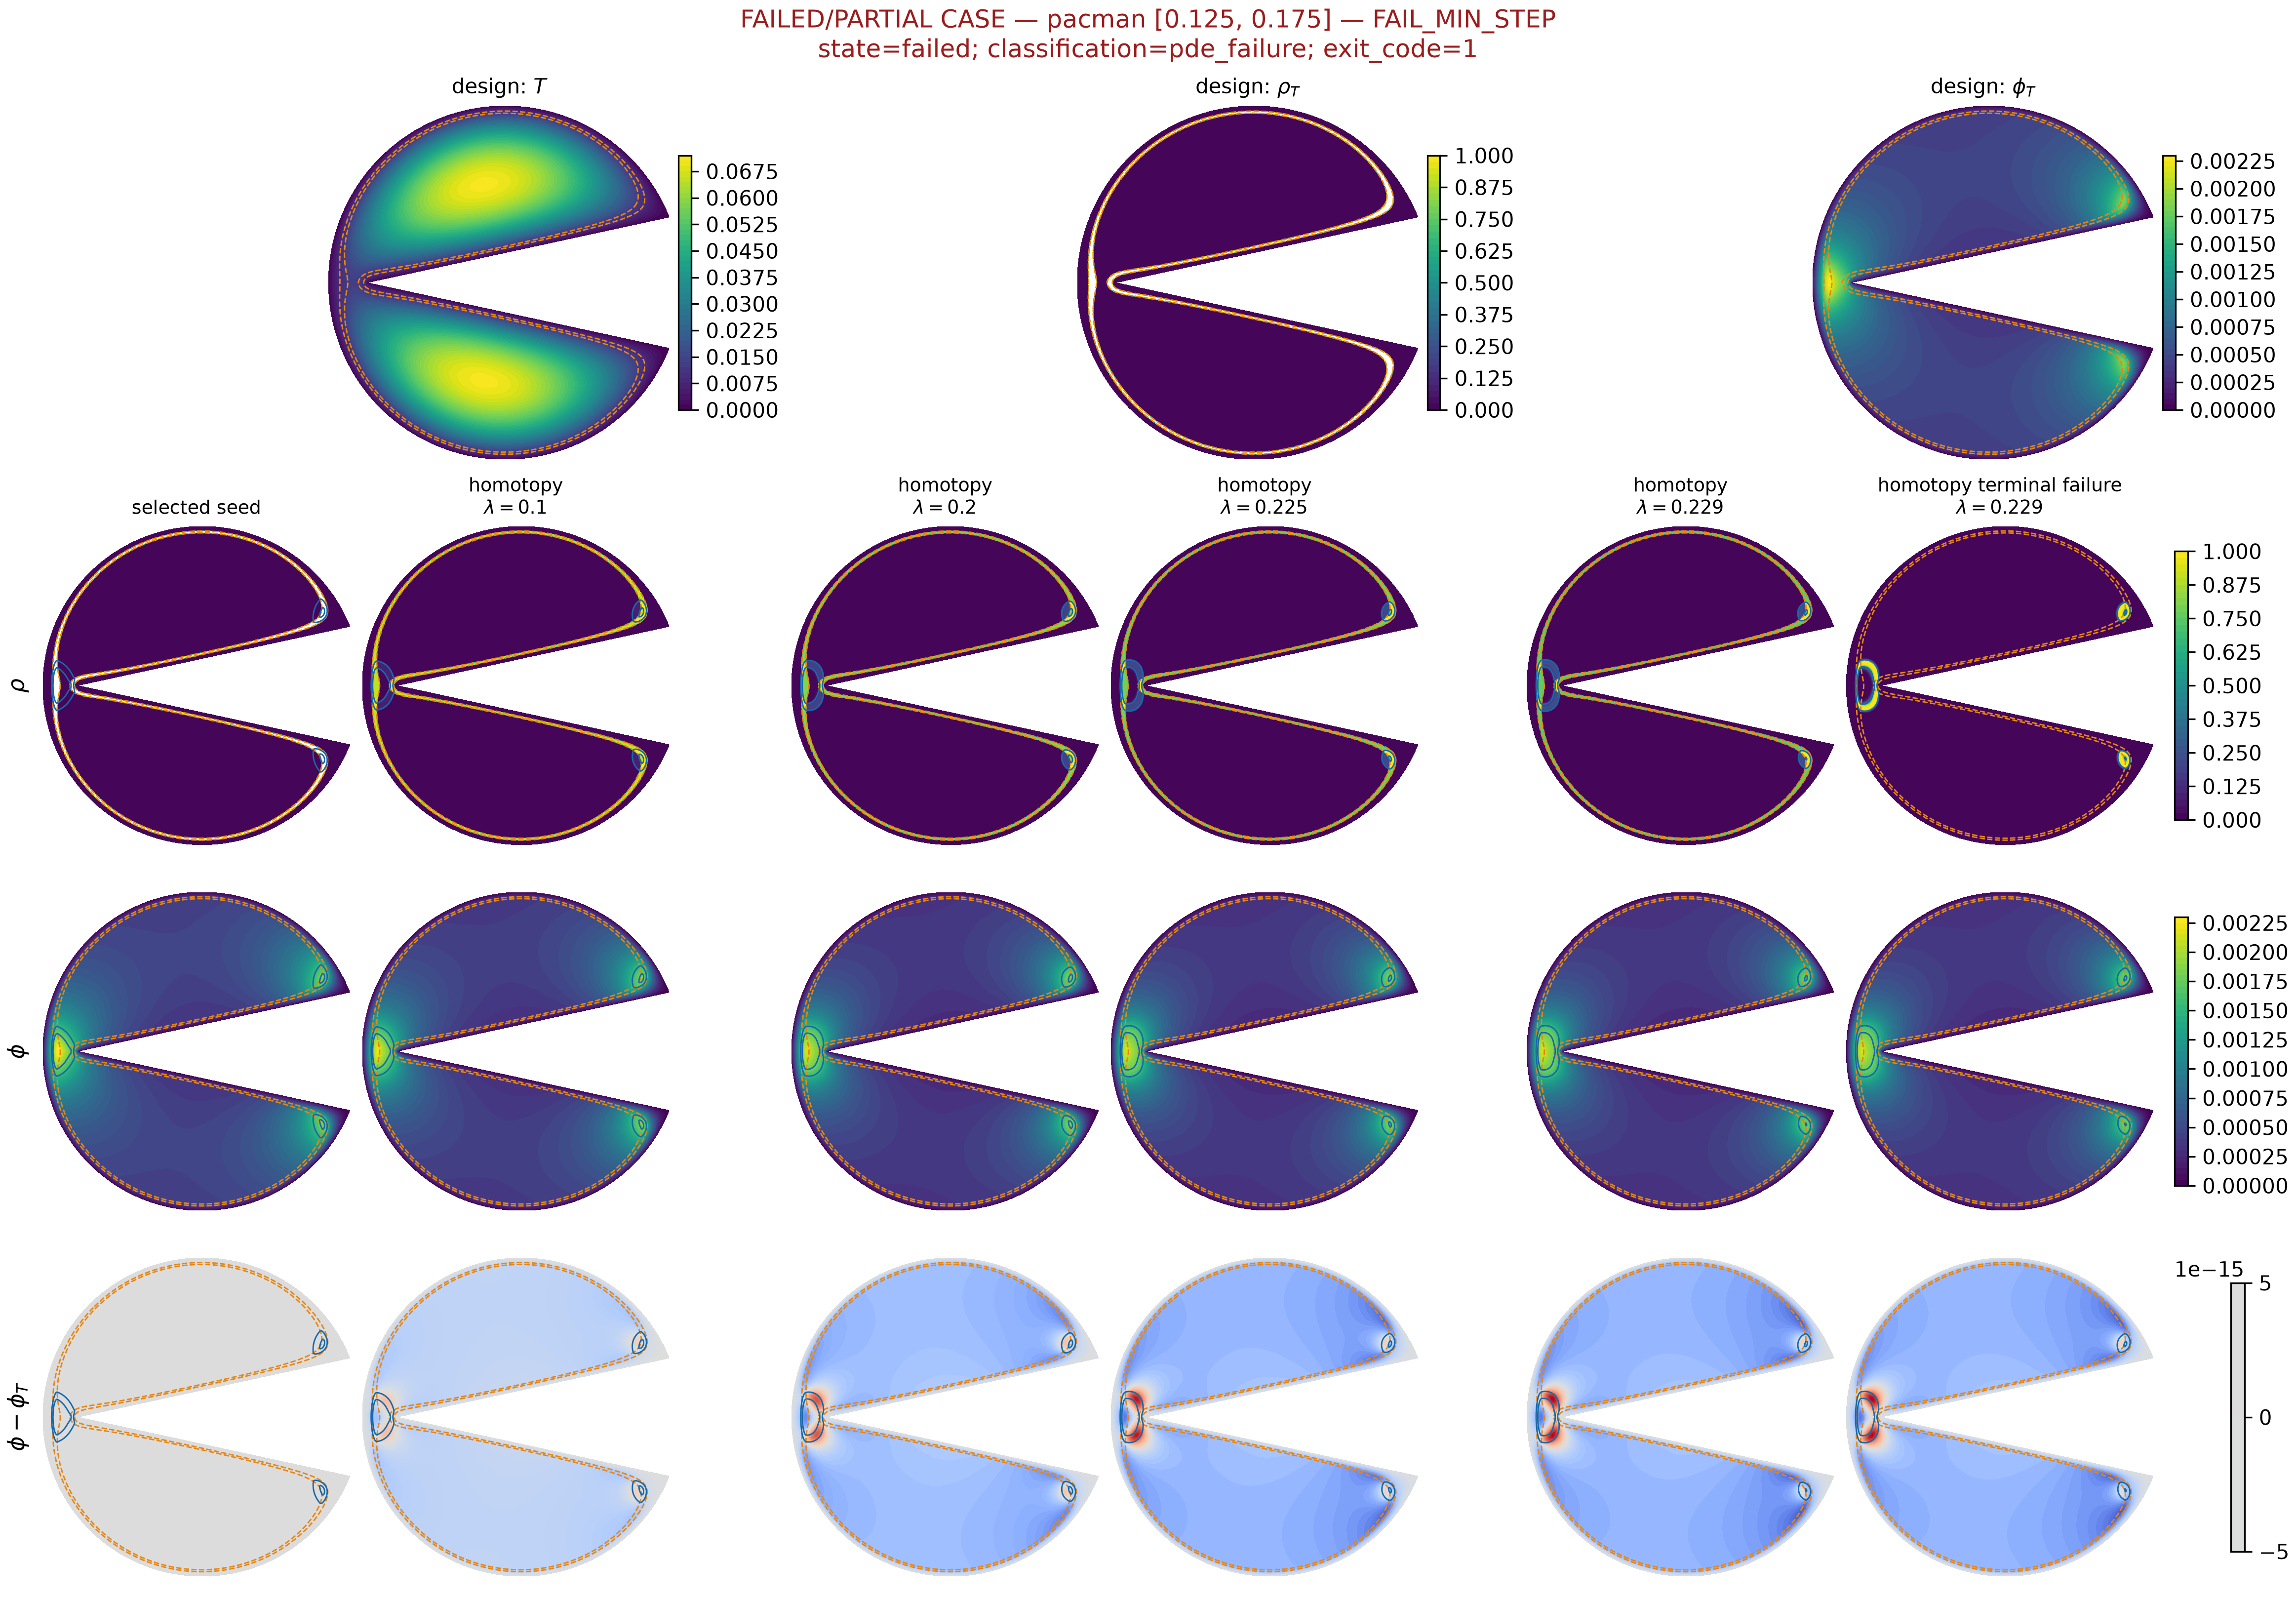
\includegraphics[width=0.88\linewidth]{figures/failed_band_evolution_012_pacman_0p125_0p175_trajectory_candidate-pacman-618faf2e713d.png}
\caption{Supplemental failed/partial trajectory evidence for pacman at torsion levels $[0.125,0.175]$ (case trajectory\_candidate-pacman-618faf2e713d; state=failed; classification=pde\_failure). The case is retained regardless of PDE or geometric success. Orange dashed curves are the fixed target band and blue solid curves are the moving equilibrium band; when state recovery is impossible, the PNG records the reason. Data status: actual.}
\label{fig:failed-storyboard-trajectory-candidate-pacman-618faf2e713d}
\end{figure}

\begin{figure}[tbp]
\centering
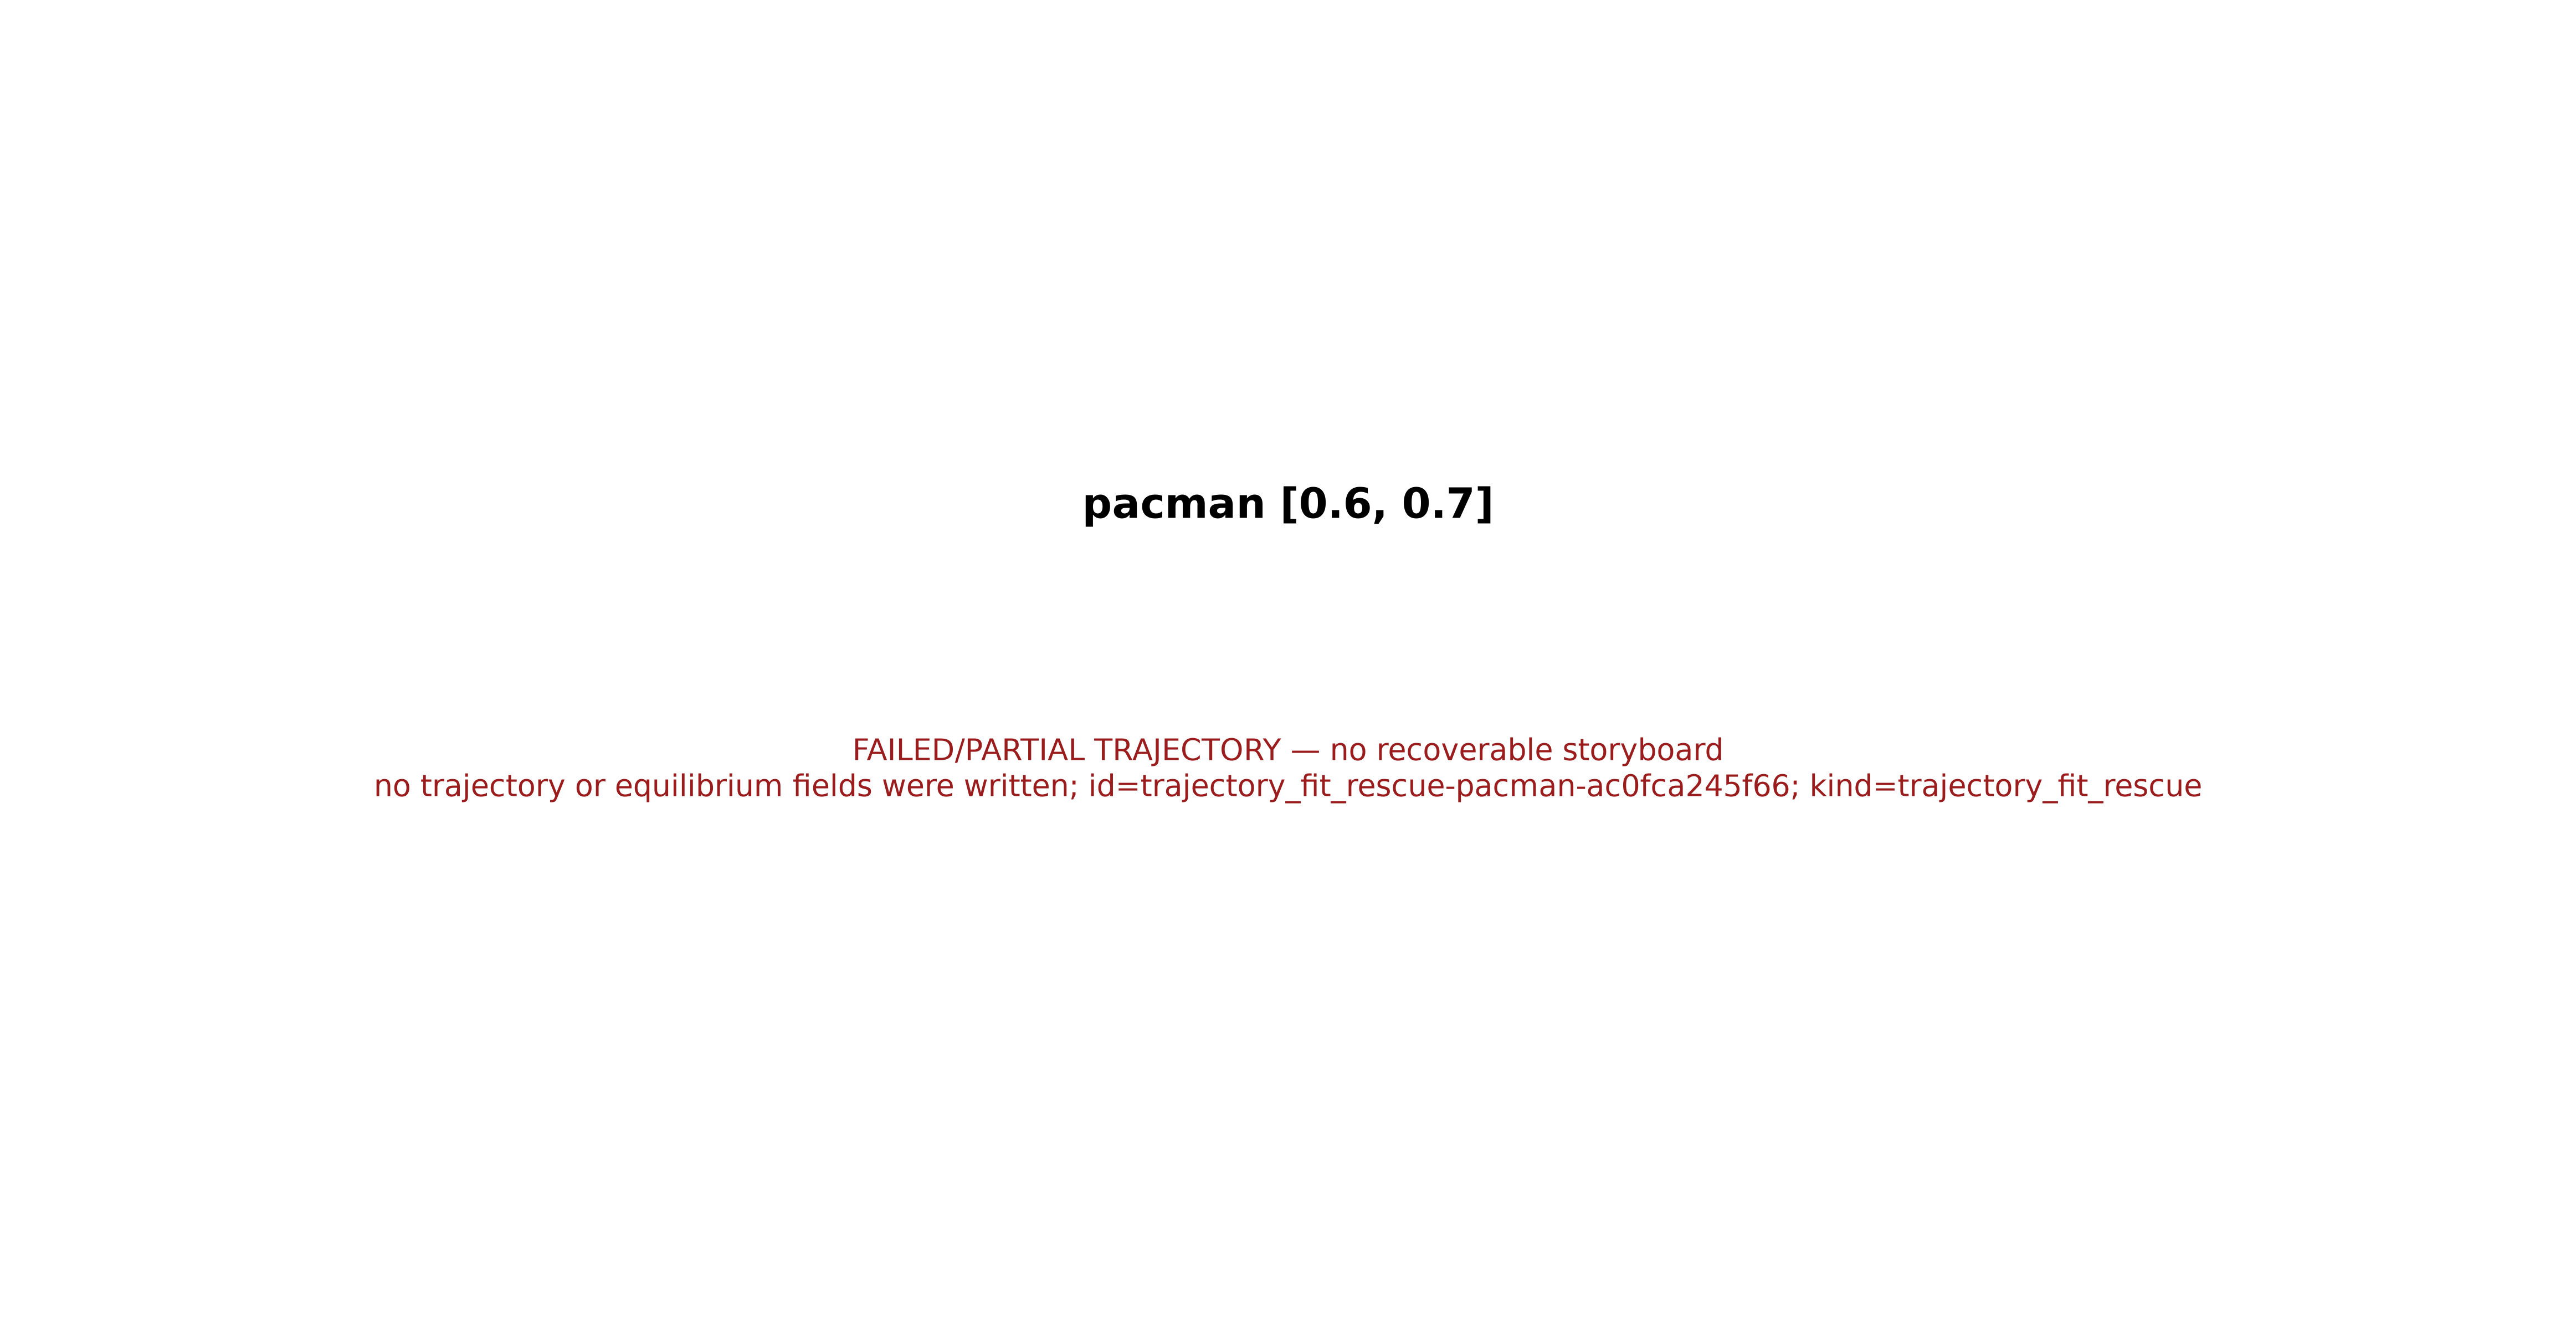
\includegraphics[width=0.88\linewidth]{figures/failed_band_evolution_013_pacman_0p6_0p7_trajectory_fit_rescue-pacman-ac0fca245f66.png}
\caption{Supplemental failed/partial trajectory evidence for pacman at torsion levels $[0.6,0.7]$ (case trajectory\_fit\_rescue-pacman-ac0fca245f66; state=deferred; classification=deferred). The case is retained regardless of PDE or geometric success. Orange dashed curves are the fixed target band and blue solid curves are the moving equilibrium band; when state recovery is impossible, the PNG records the reason. Data status: diagnostic\_only.}
\label{fig:failed-storyboard-trajectory-fit-rescue-pacman-ac0fca245f66}
\end{figure}

\clearpage

\begin{figure}[tbp]
\centering
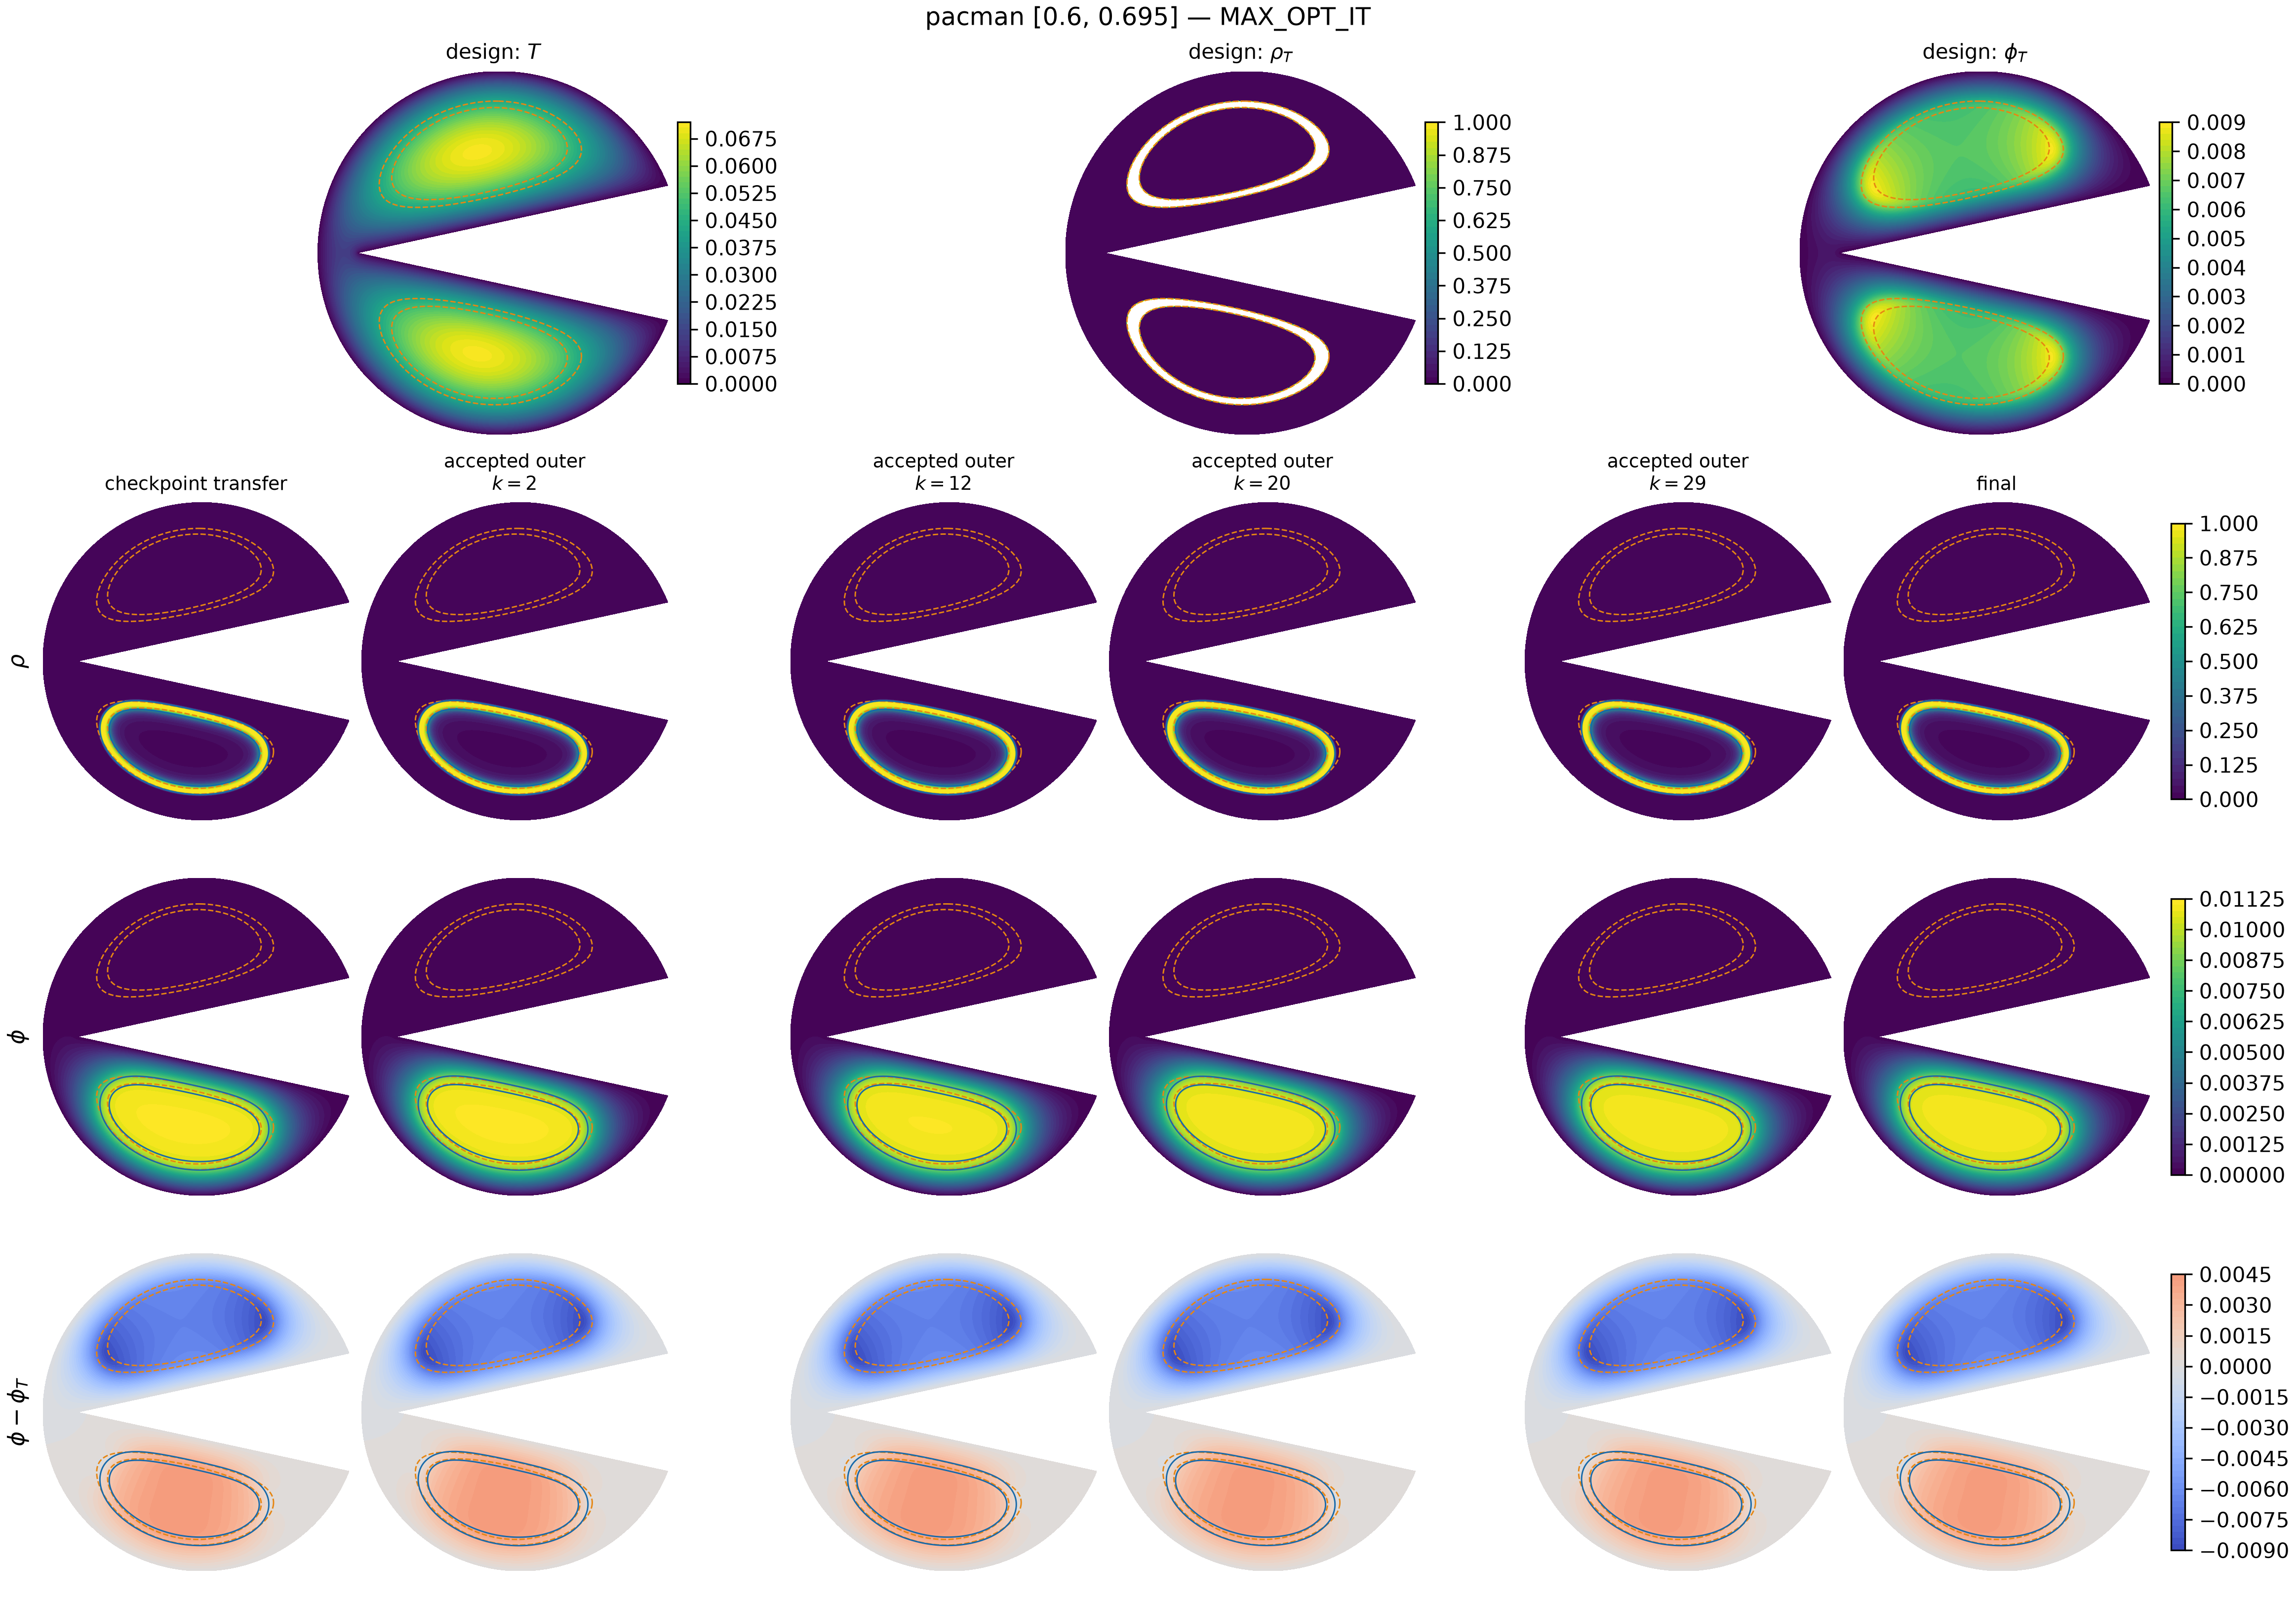
\includegraphics[width=0.88\linewidth]{figures/failed_band_evolution_014_pacman_0p6_0p695_trajectory_v3-pacman-4d5357771618.png}
\caption{Supplemental failed/partial trajectory evidence for pacman at torsion levels $[0.6,0.695]$ (case trajectory\_v3-pacman-4d5357771618; state=completed; classification=geometrically\_unsuccessful\_pde\_converged). The case is retained regardless of PDE or geometric success. Orange dashed curves are the fixed target band and blue solid curves are the moving equilibrium band; when state recovery is impossible, the PNG records the reason. Data status: actual.}
\label{fig:failed-storyboard-trajectory-v3-pacman-4d5357771618}
\end{figure}

\begin{figure}[tbp]
\centering
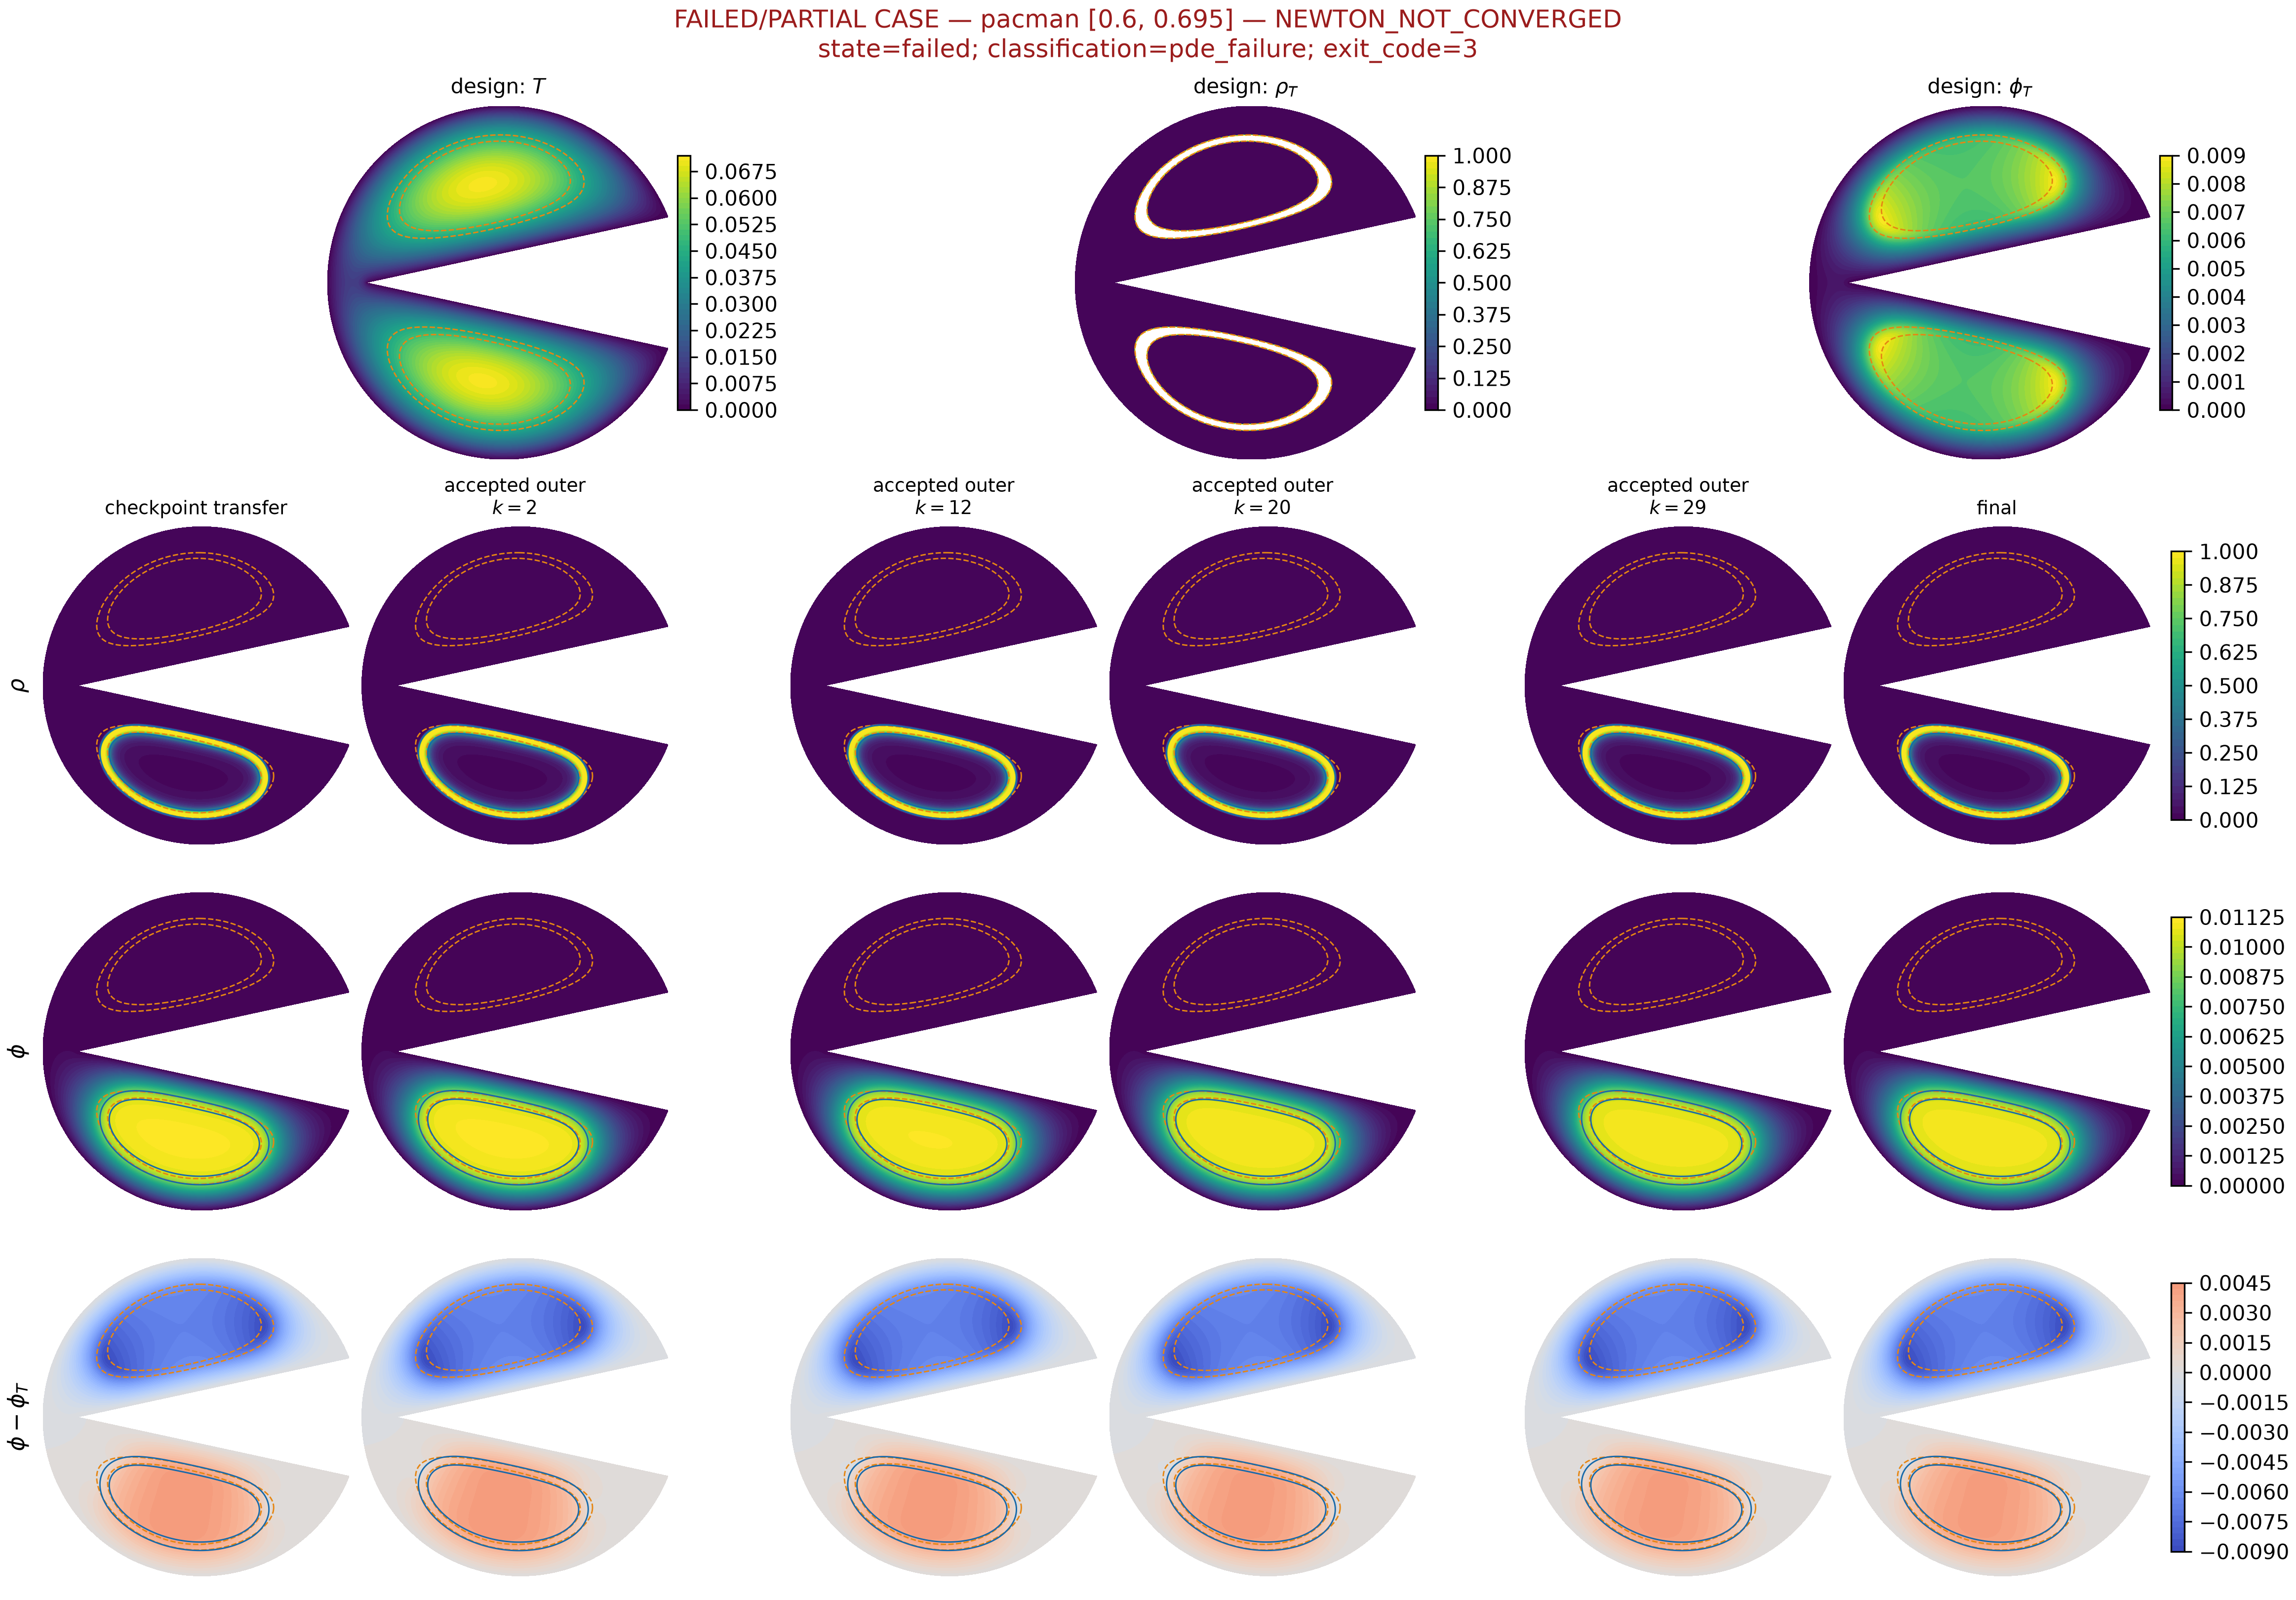
\includegraphics[width=0.88\linewidth]{figures/failed_band_evolution_015_pacman_0p6_0p695_trajectory_v3-pacman-822f380f34d3.png}
\caption{Supplemental failed/partial trajectory evidence for pacman at torsion levels $[0.6,0.695]$ (case trajectory\_v3-pacman-822f380f34d3; state=failed; classification=pde\_failure). The case is retained regardless of PDE or geometric success. Orange dashed curves are the fixed target band and blue solid curves are the moving equilibrium band; when state recovery is impossible, the PNG records the reason. Data status: actual.}
\label{fig:failed-storyboard-trajectory-v3-pacman-822f380f34d3}
\end{figure}

\begin{figure}[tbp]
\centering
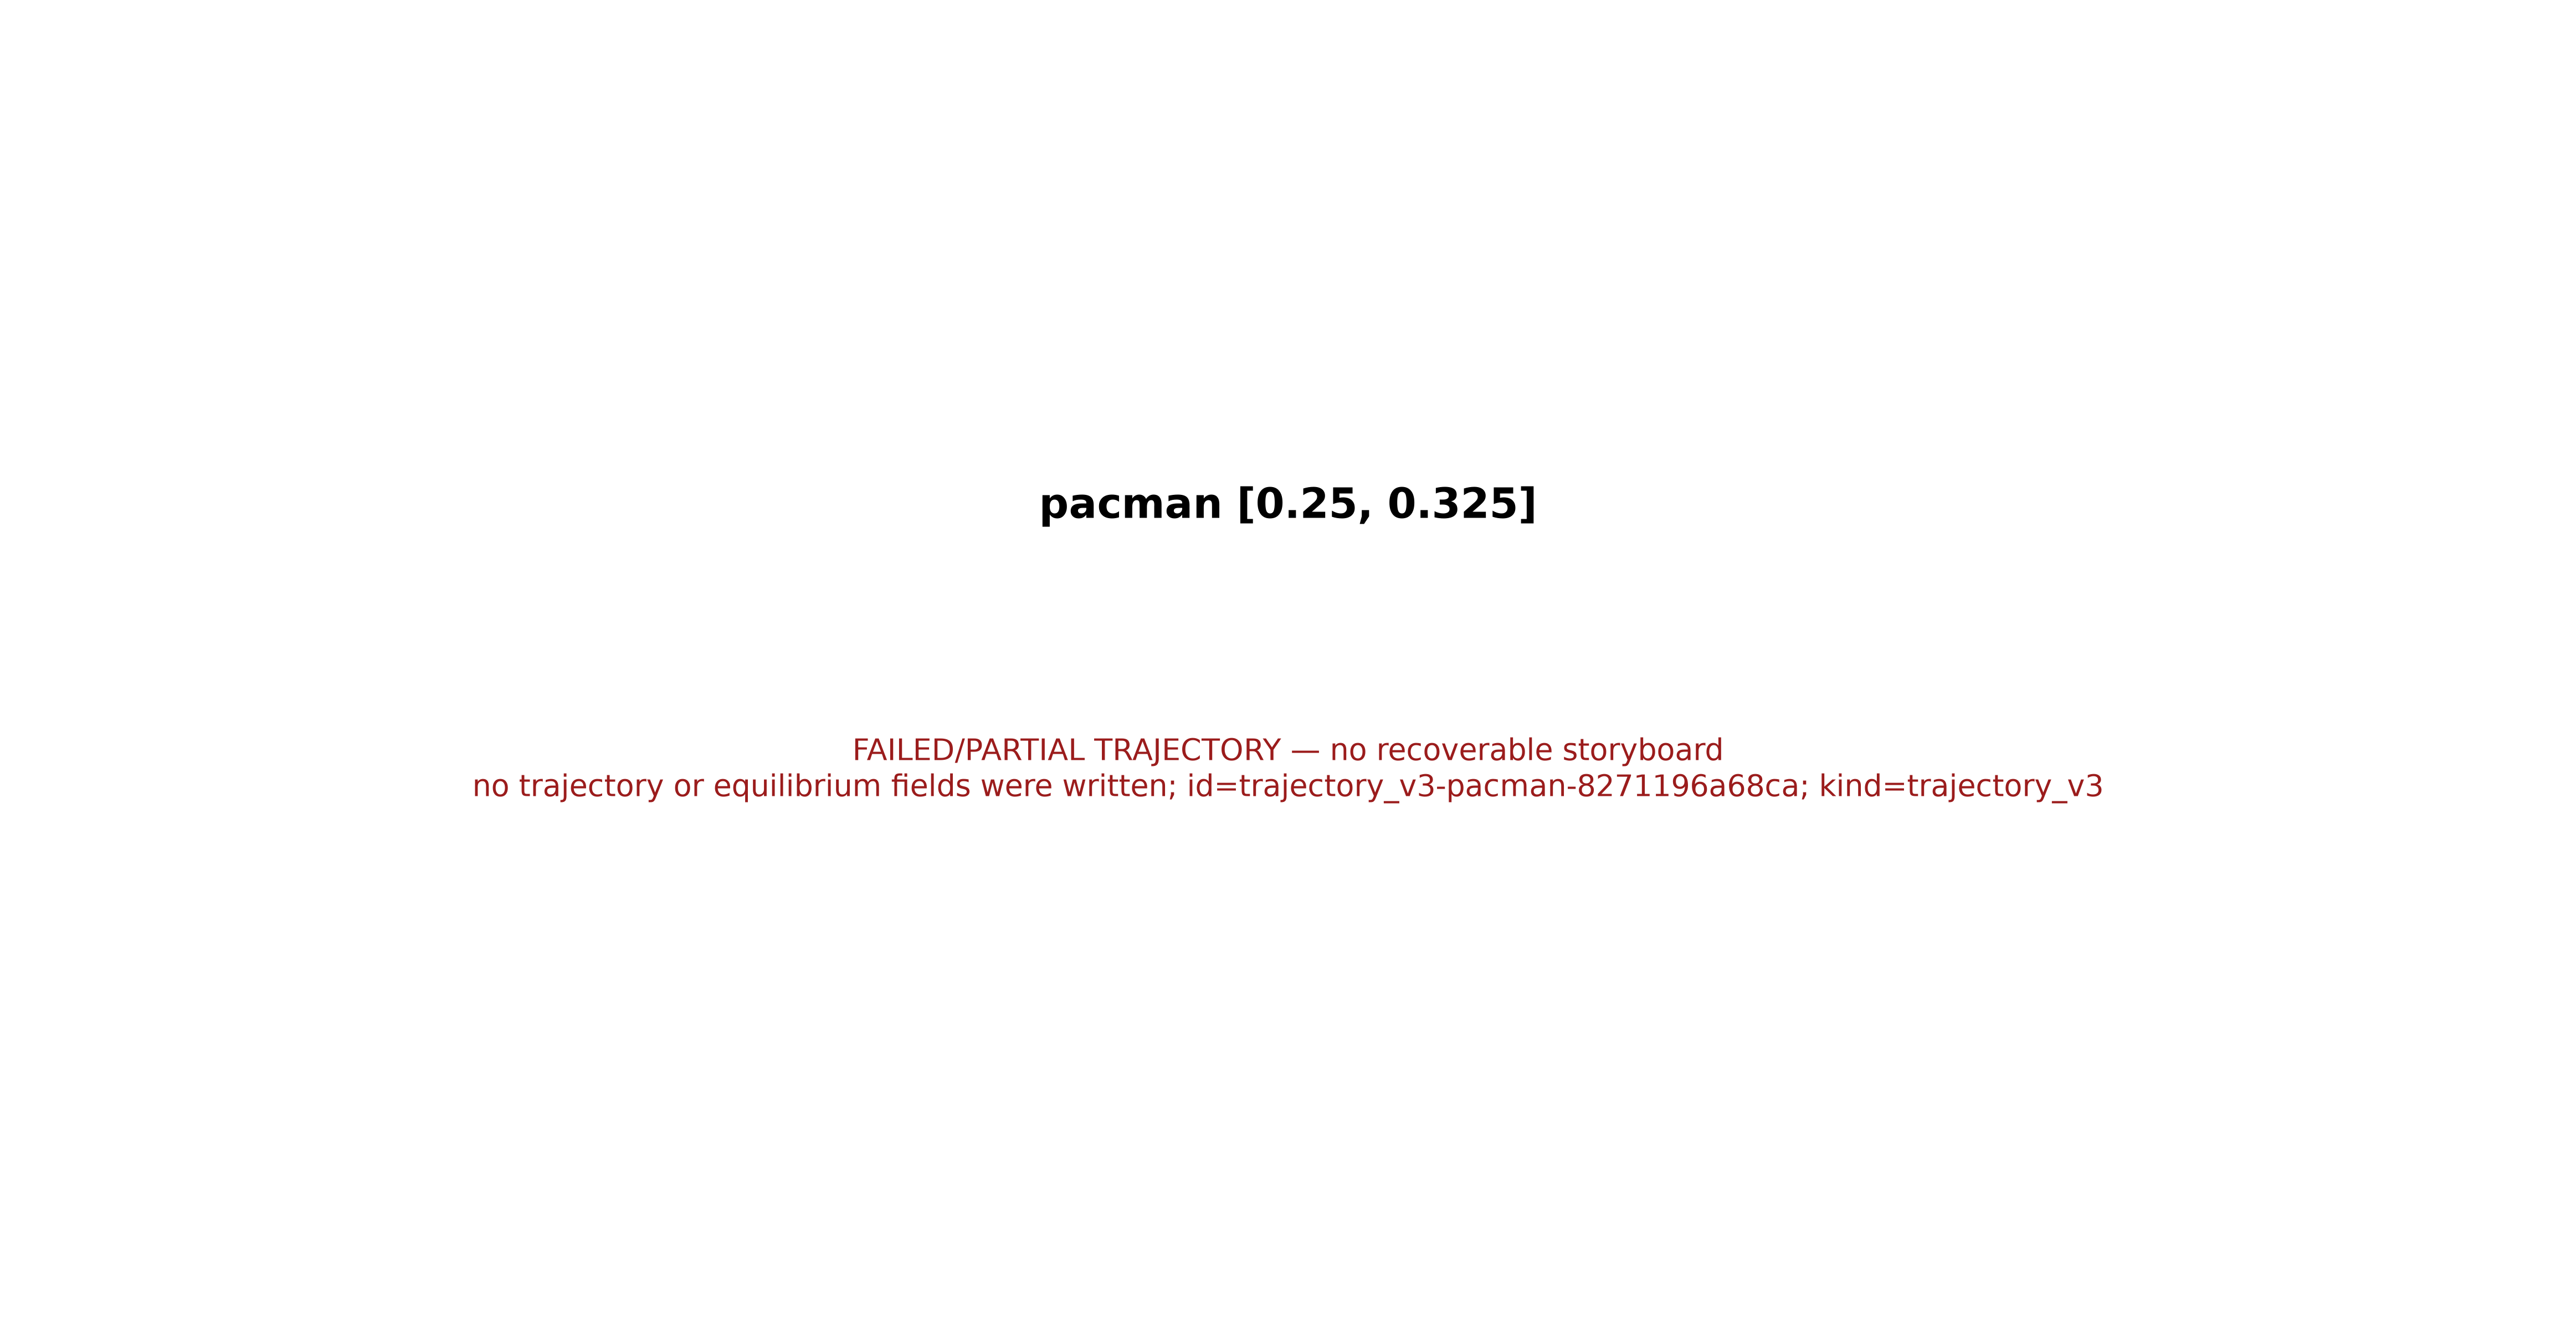
\includegraphics[width=0.88\linewidth]{figures/failed_band_evolution_016_pacman_0p25_0p325_trajectory_v3-pacman-8271196a68ca.png}
\caption{Supplemental failed/partial trajectory evidence for pacman at torsion levels $[0.25,0.325]$ (case trajectory\_v3-pacman-8271196a68ca; state=deferred; classification=deferred). The case is retained regardless of PDE or geometric success. Orange dashed curves are the fixed target band and blue solid curves are the moving equilibrium band; when state recovery is impossible, the PNG records the reason. Data status: diagnostic\_only.}
\label{fig:failed-storyboard-trajectory-v3-pacman-8271196a68ca}
\end{figure}

\begin{figure}[tbp]
\centering
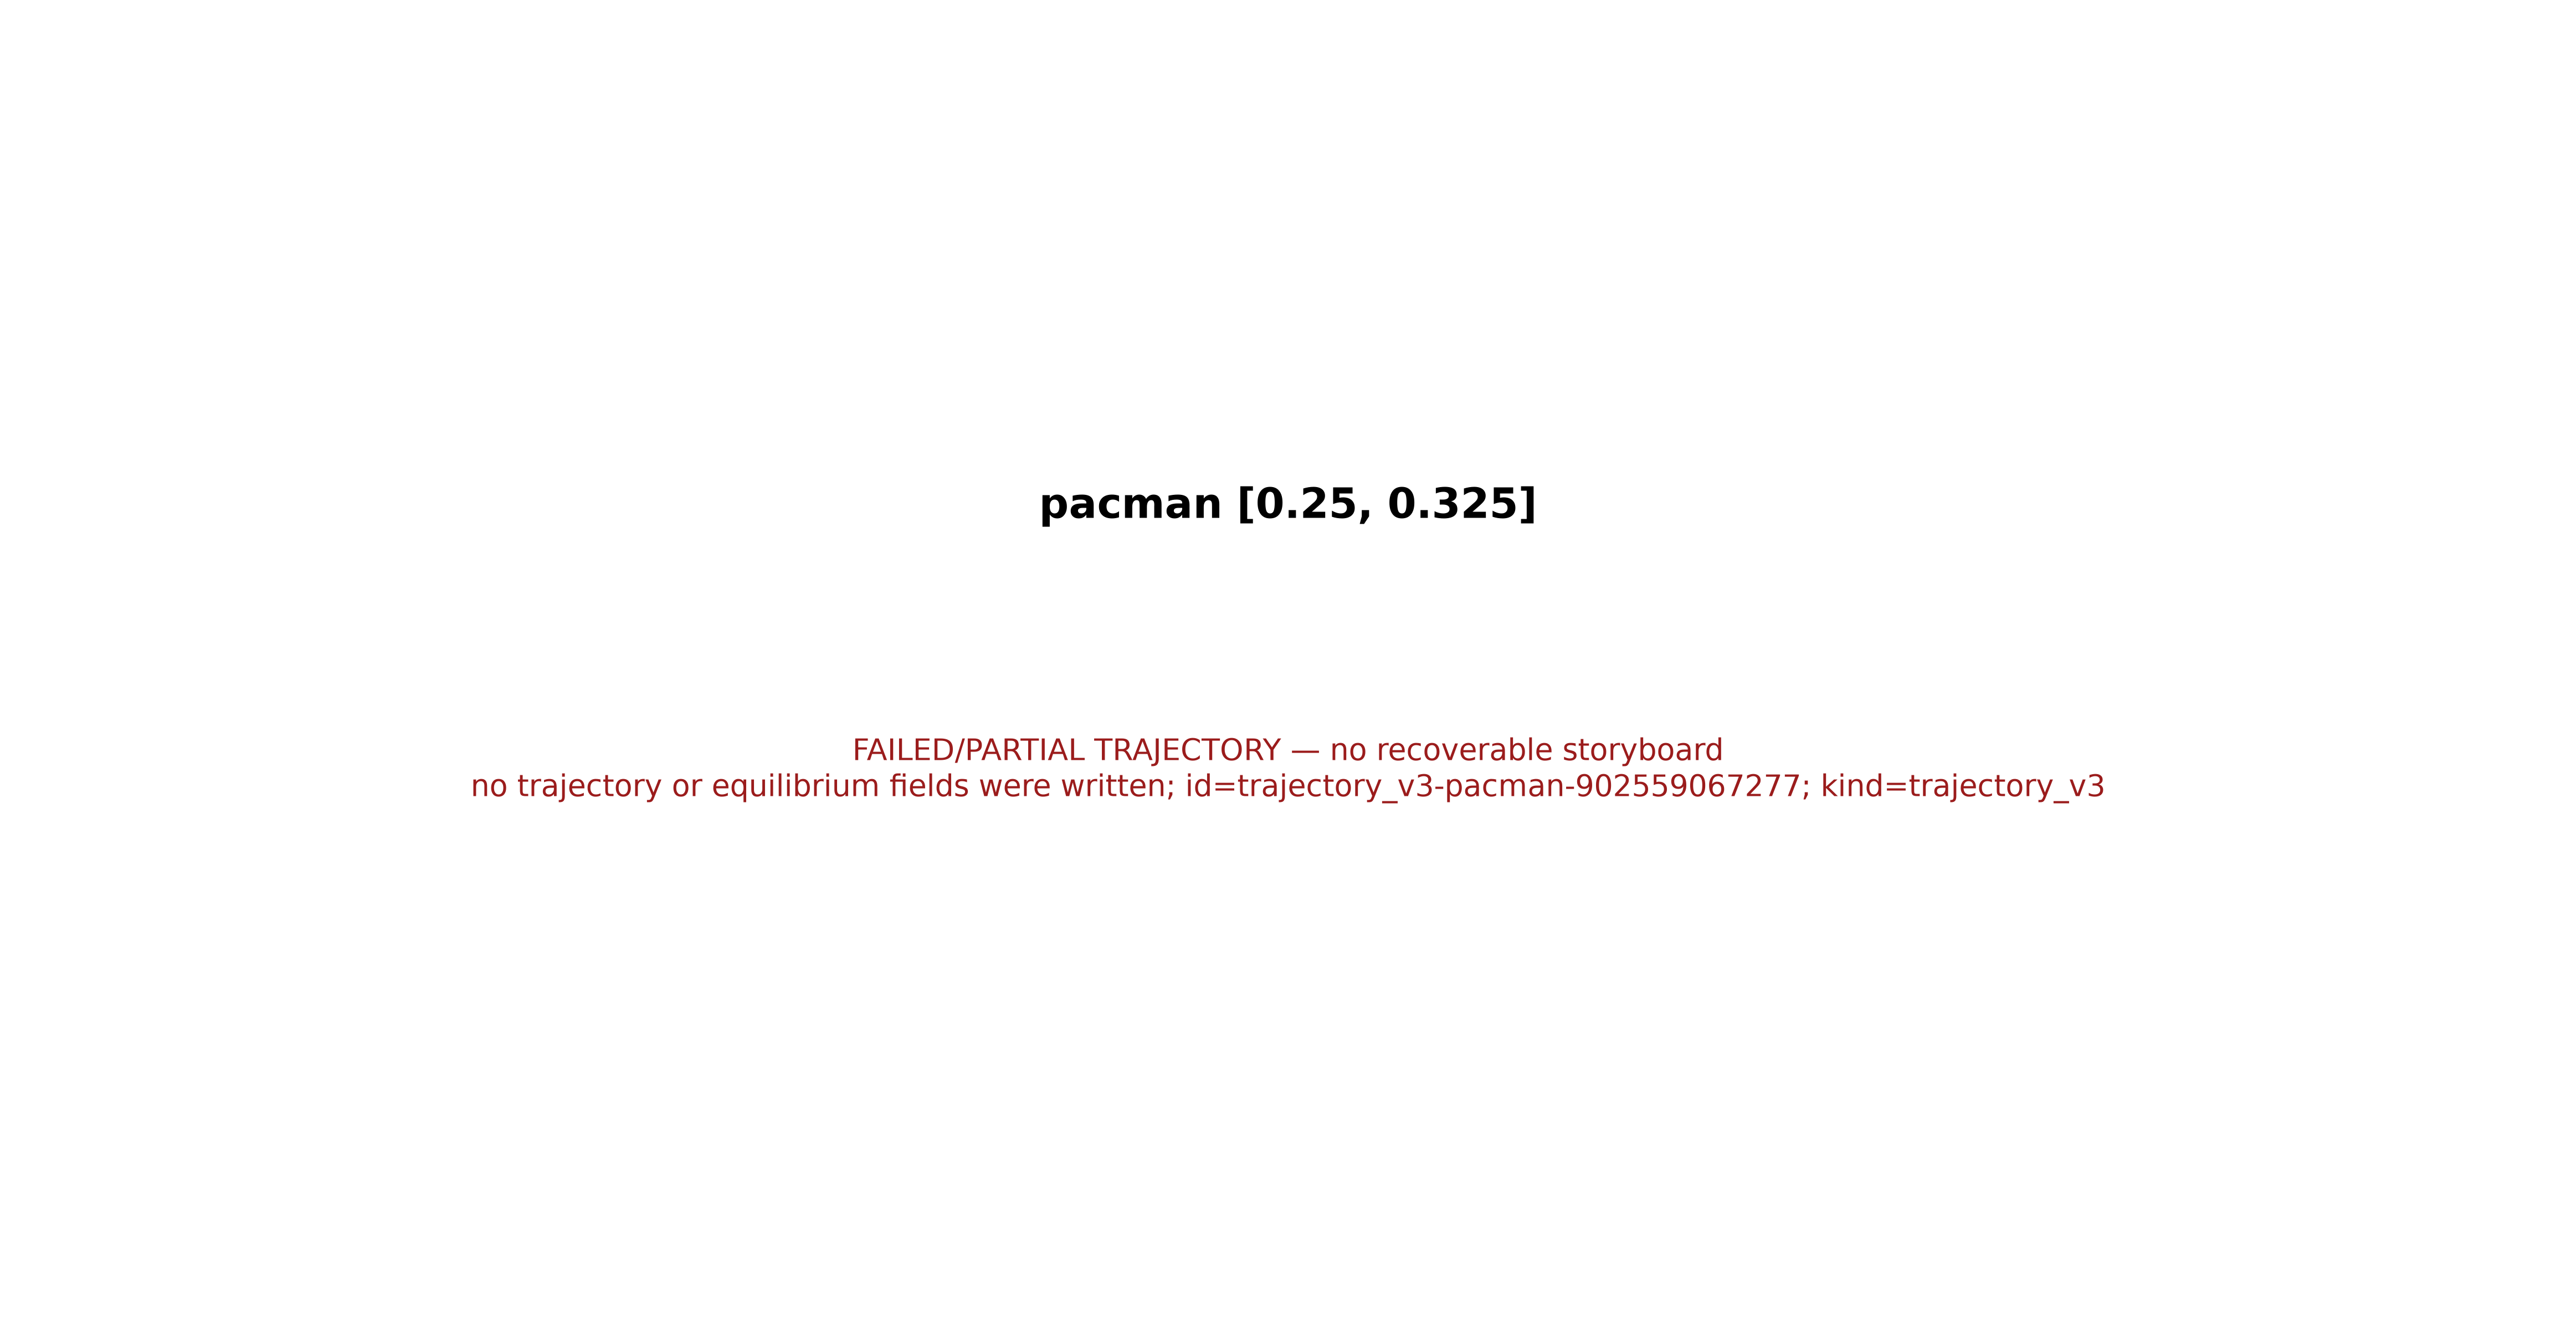
\includegraphics[width=0.88\linewidth]{figures/failed_band_evolution_017_pacman_0p25_0p325_trajectory_v3-pacman-902559067277.png}
\caption{Supplemental failed/partial trajectory evidence for pacman at torsion levels $[0.25,0.325]$ (case trajectory\_v3-pacman-902559067277; state=deferred; classification=deferred). The case is retained regardless of PDE or geometric success. Orange dashed curves are the fixed target band and blue solid curves are the moving equilibrium band; when state recovery is impossible, the PNG records the reason. Data status: diagnostic\_only.}
\label{fig:failed-storyboard-trajectory-v3-pacman-902559067277}
\end{figure}

\begin{figure}[tbp]
\centering
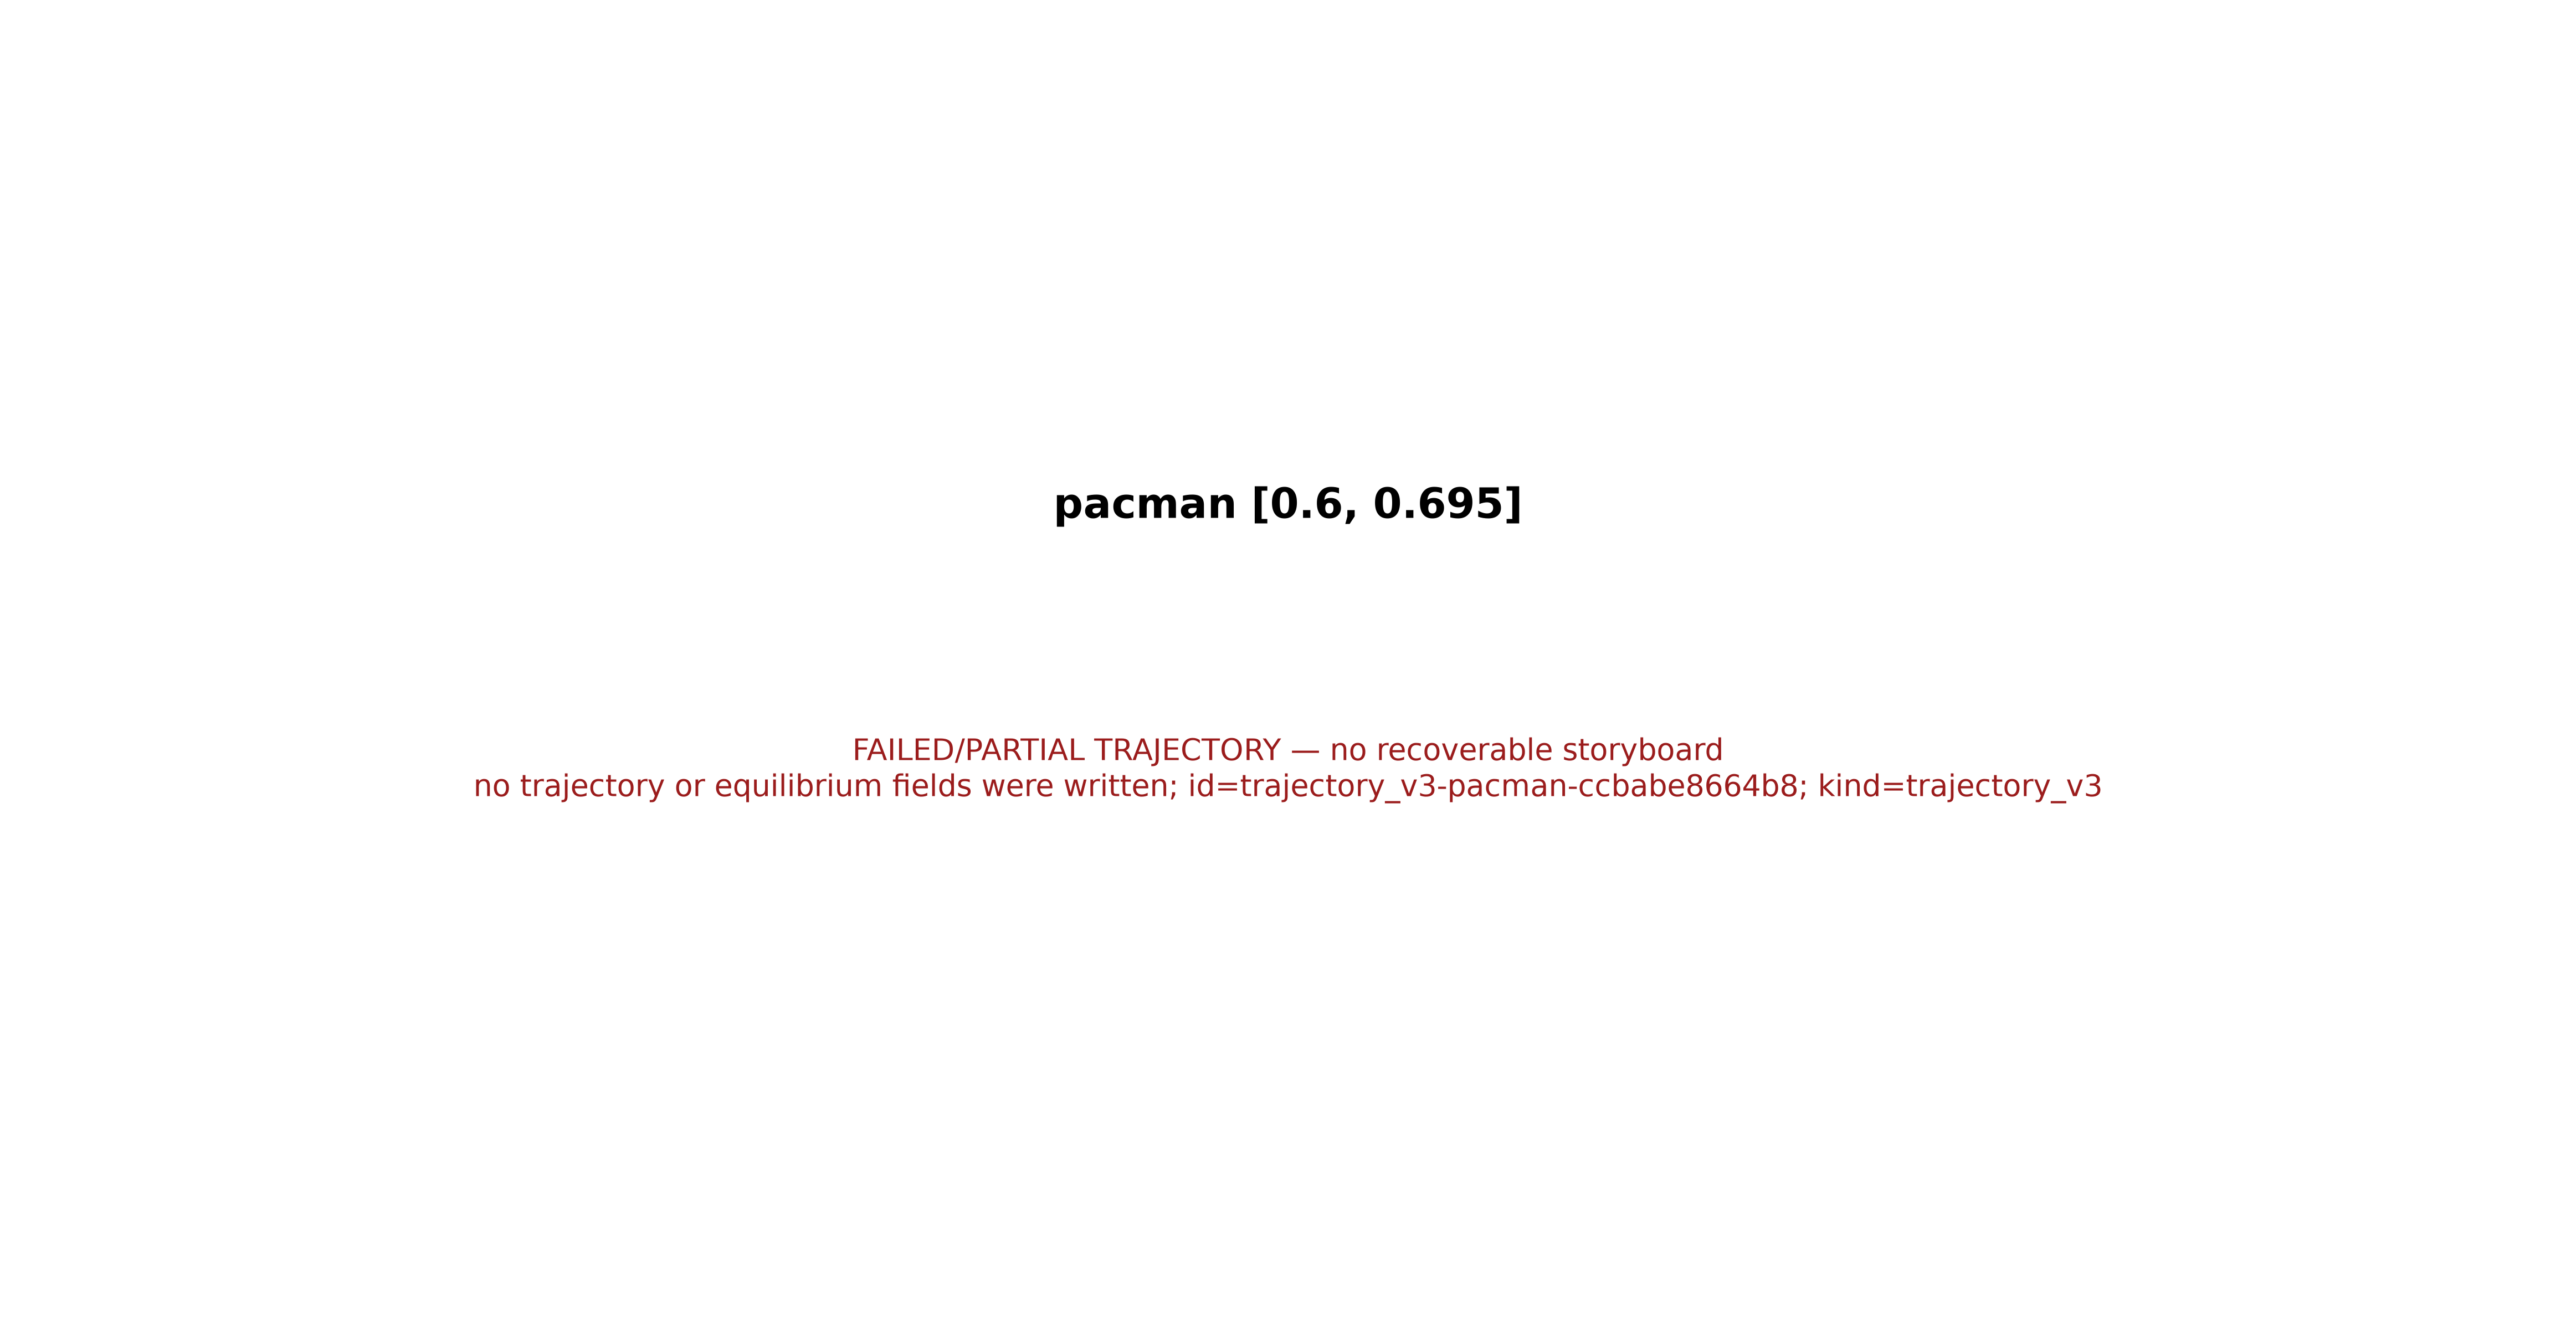
\includegraphics[width=0.88\linewidth]{figures/failed_band_evolution_018_pacman_0p6_0p695_trajectory_v3-pacman-ccbabe8664b8.png}
\caption{Supplemental failed/partial trajectory evidence for pacman at torsion levels $[0.6,0.695]$ (case trajectory\_v3-pacman-ccbabe8664b8; state=deferred; classification=deferred). The case is retained regardless of PDE or geometric success. Orange dashed curves are the fixed target band and blue solid curves are the moving equilibrium band; when state recovery is impossible, the PNG records the reason. Data status: diagnostic\_only.}
\label{fig:failed-storyboard-trajectory-v3-pacman-ccbabe8664b8}
\end{figure}

\begin{figure}[tbp]
\centering
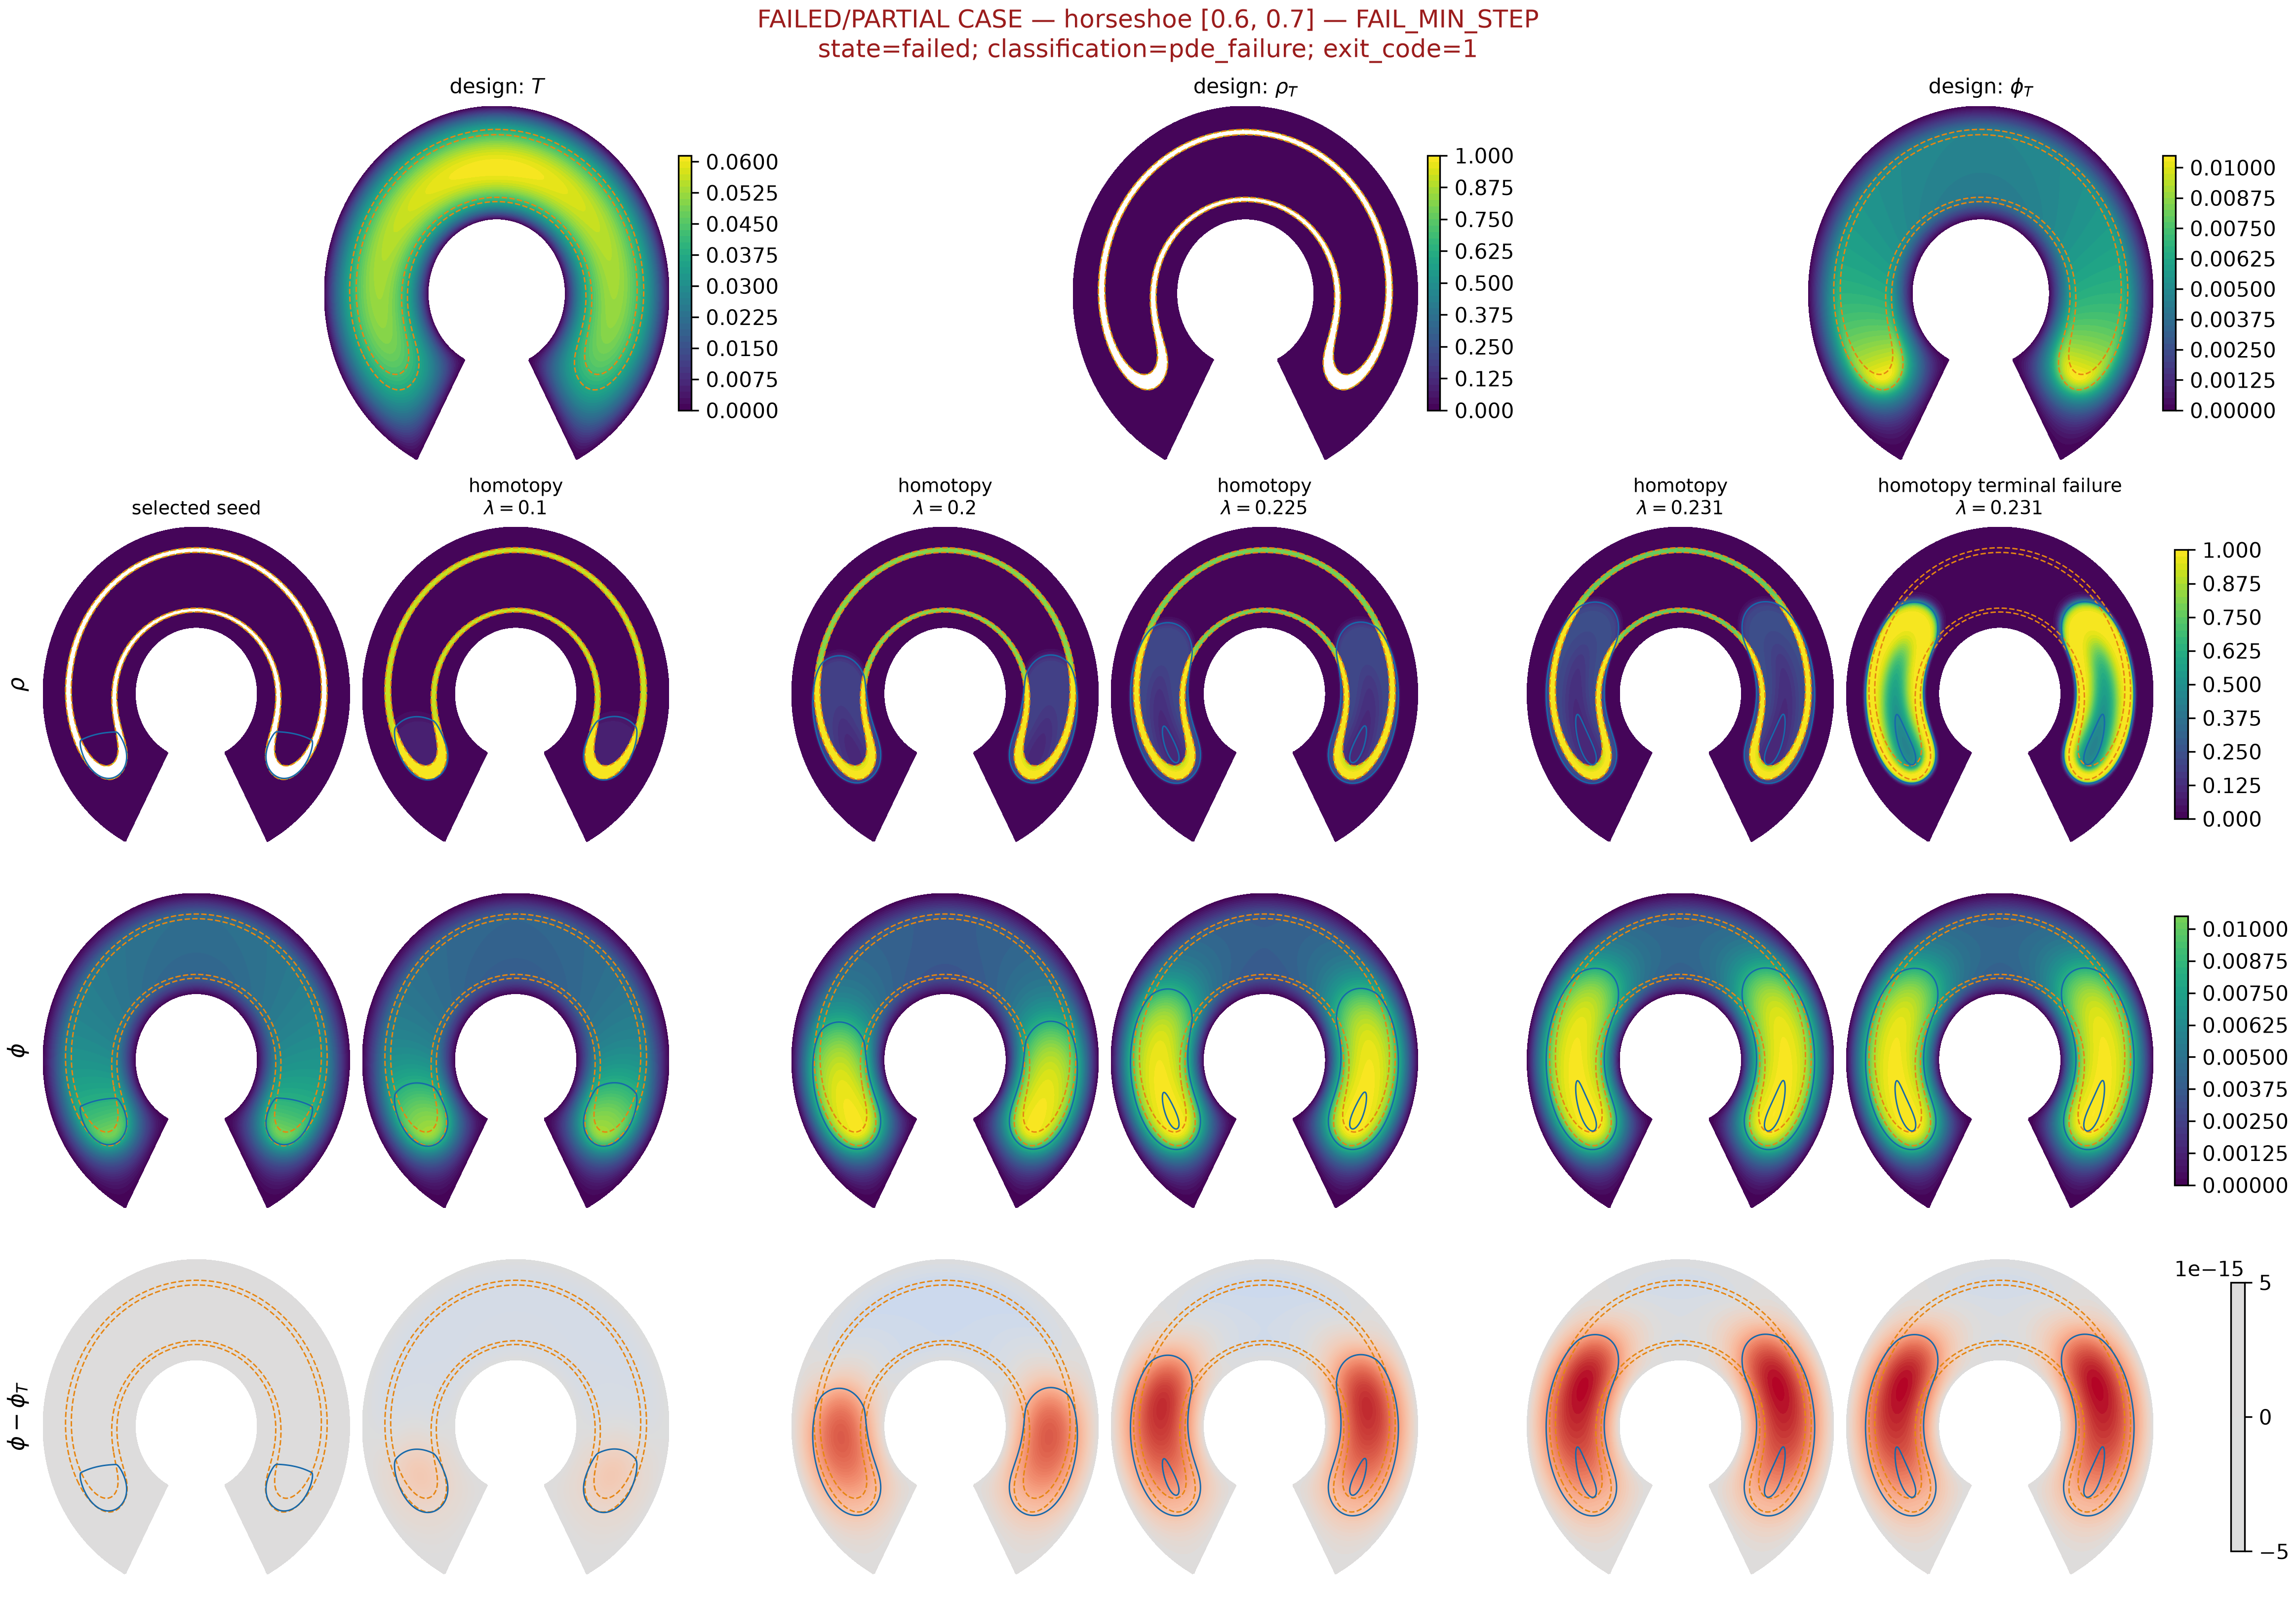
\includegraphics[width=0.88\linewidth]{figures/failed_band_evolution_019_horseshoe_0p6_0p7_trajectory-horseshoe-2d70b6ab8bf2.png}
\caption{Supplemental failed/partial trajectory evidence for horseshoe at torsion levels $[0.6,0.7]$ (case trajectory-horseshoe-2d70b6ab8bf2; state=failed; classification=pde\_failure). The case is retained regardless of PDE or geometric success. Orange dashed curves are the fixed target band and blue solid curves are the moving equilibrium band; when state recovery is impossible, the PNG records the reason. Data status: actual.}
\label{fig:failed-storyboard-trajectory-horseshoe-2d70b6ab8bf2}
\end{figure}

\begin{figure}[tbp]
\centering
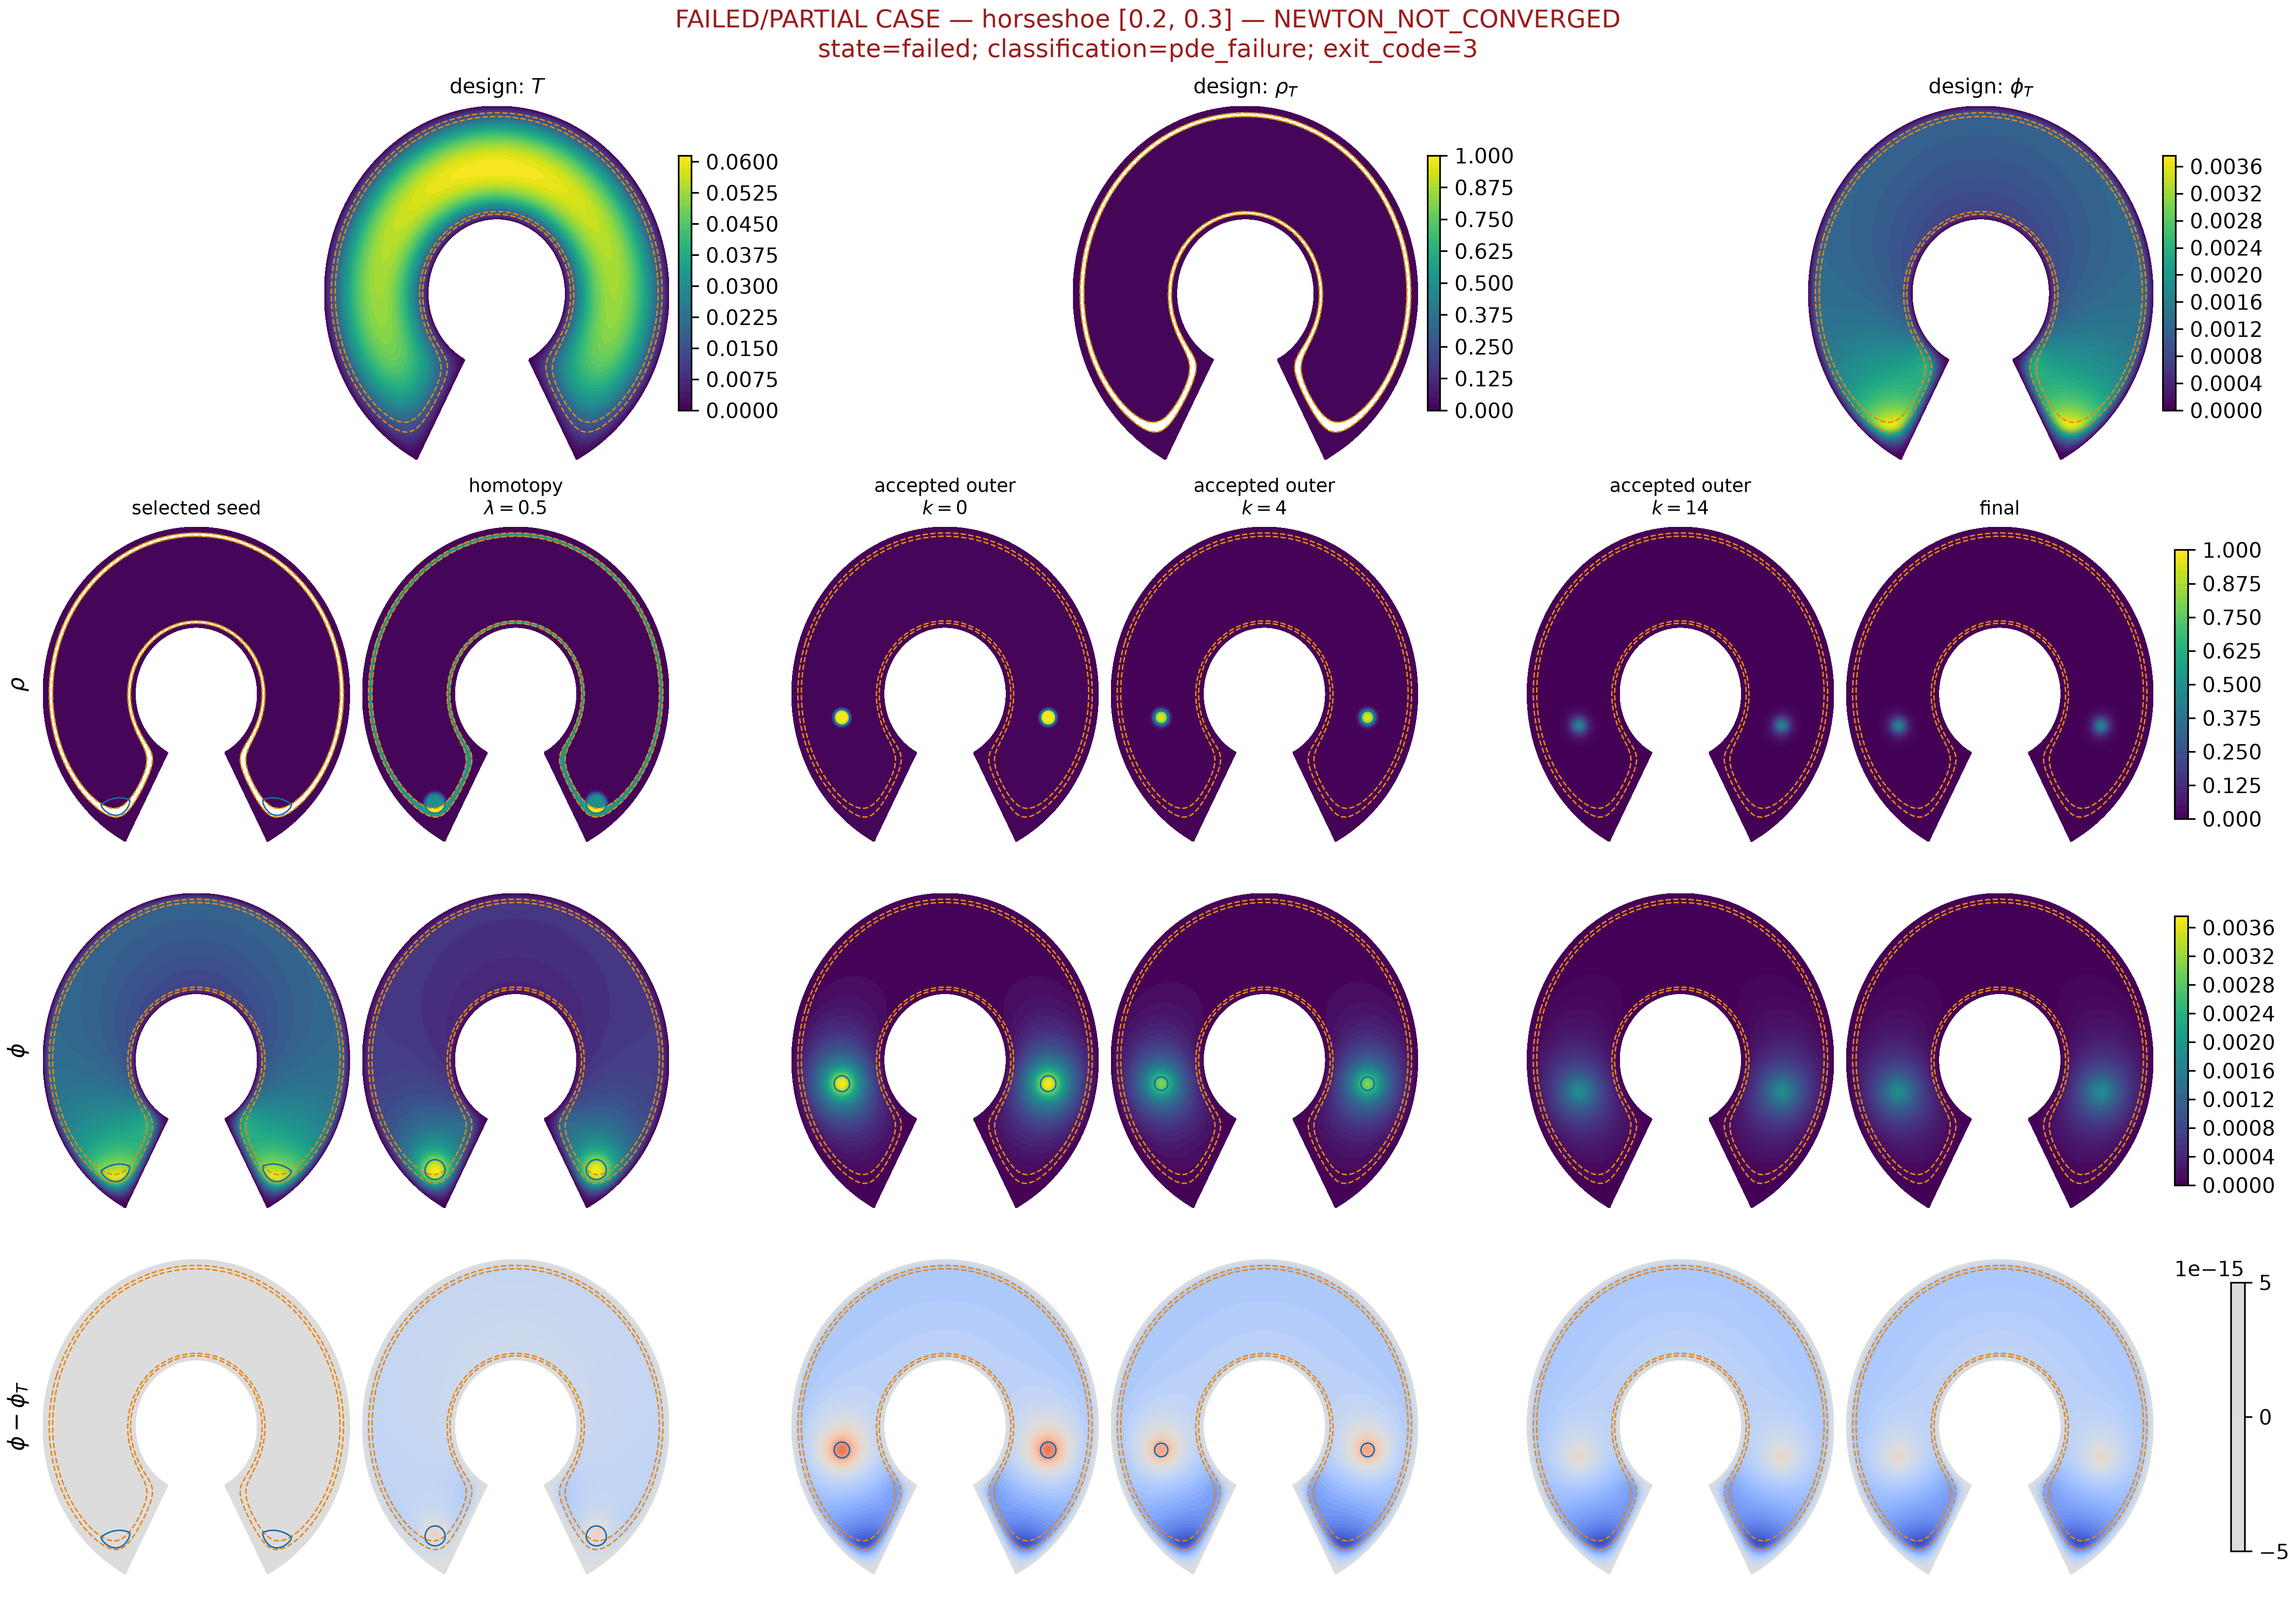
\includegraphics[width=0.88\linewidth]{figures/failed_band_evolution_020_horseshoe_0p2_0p3_trajectory_candidate-horseshoe-0ece12c40d74.png}
\caption{Supplemental failed/partial trajectory evidence for horseshoe at torsion levels $[0.2,0.3]$ (case trajectory\_candidate-horseshoe-0ece12c40d74; state=failed; classification=pde\_failure). The case is retained regardless of PDE or geometric success. Orange dashed curves are the fixed target band and blue solid curves are the moving equilibrium band; when state recovery is impossible, the PNG records the reason. Data status: actual.}
\label{fig:failed-storyboard-trajectory-candidate-horseshoe-0ece12c40d74}
\end{figure}

\begin{figure}[tbp]
\centering
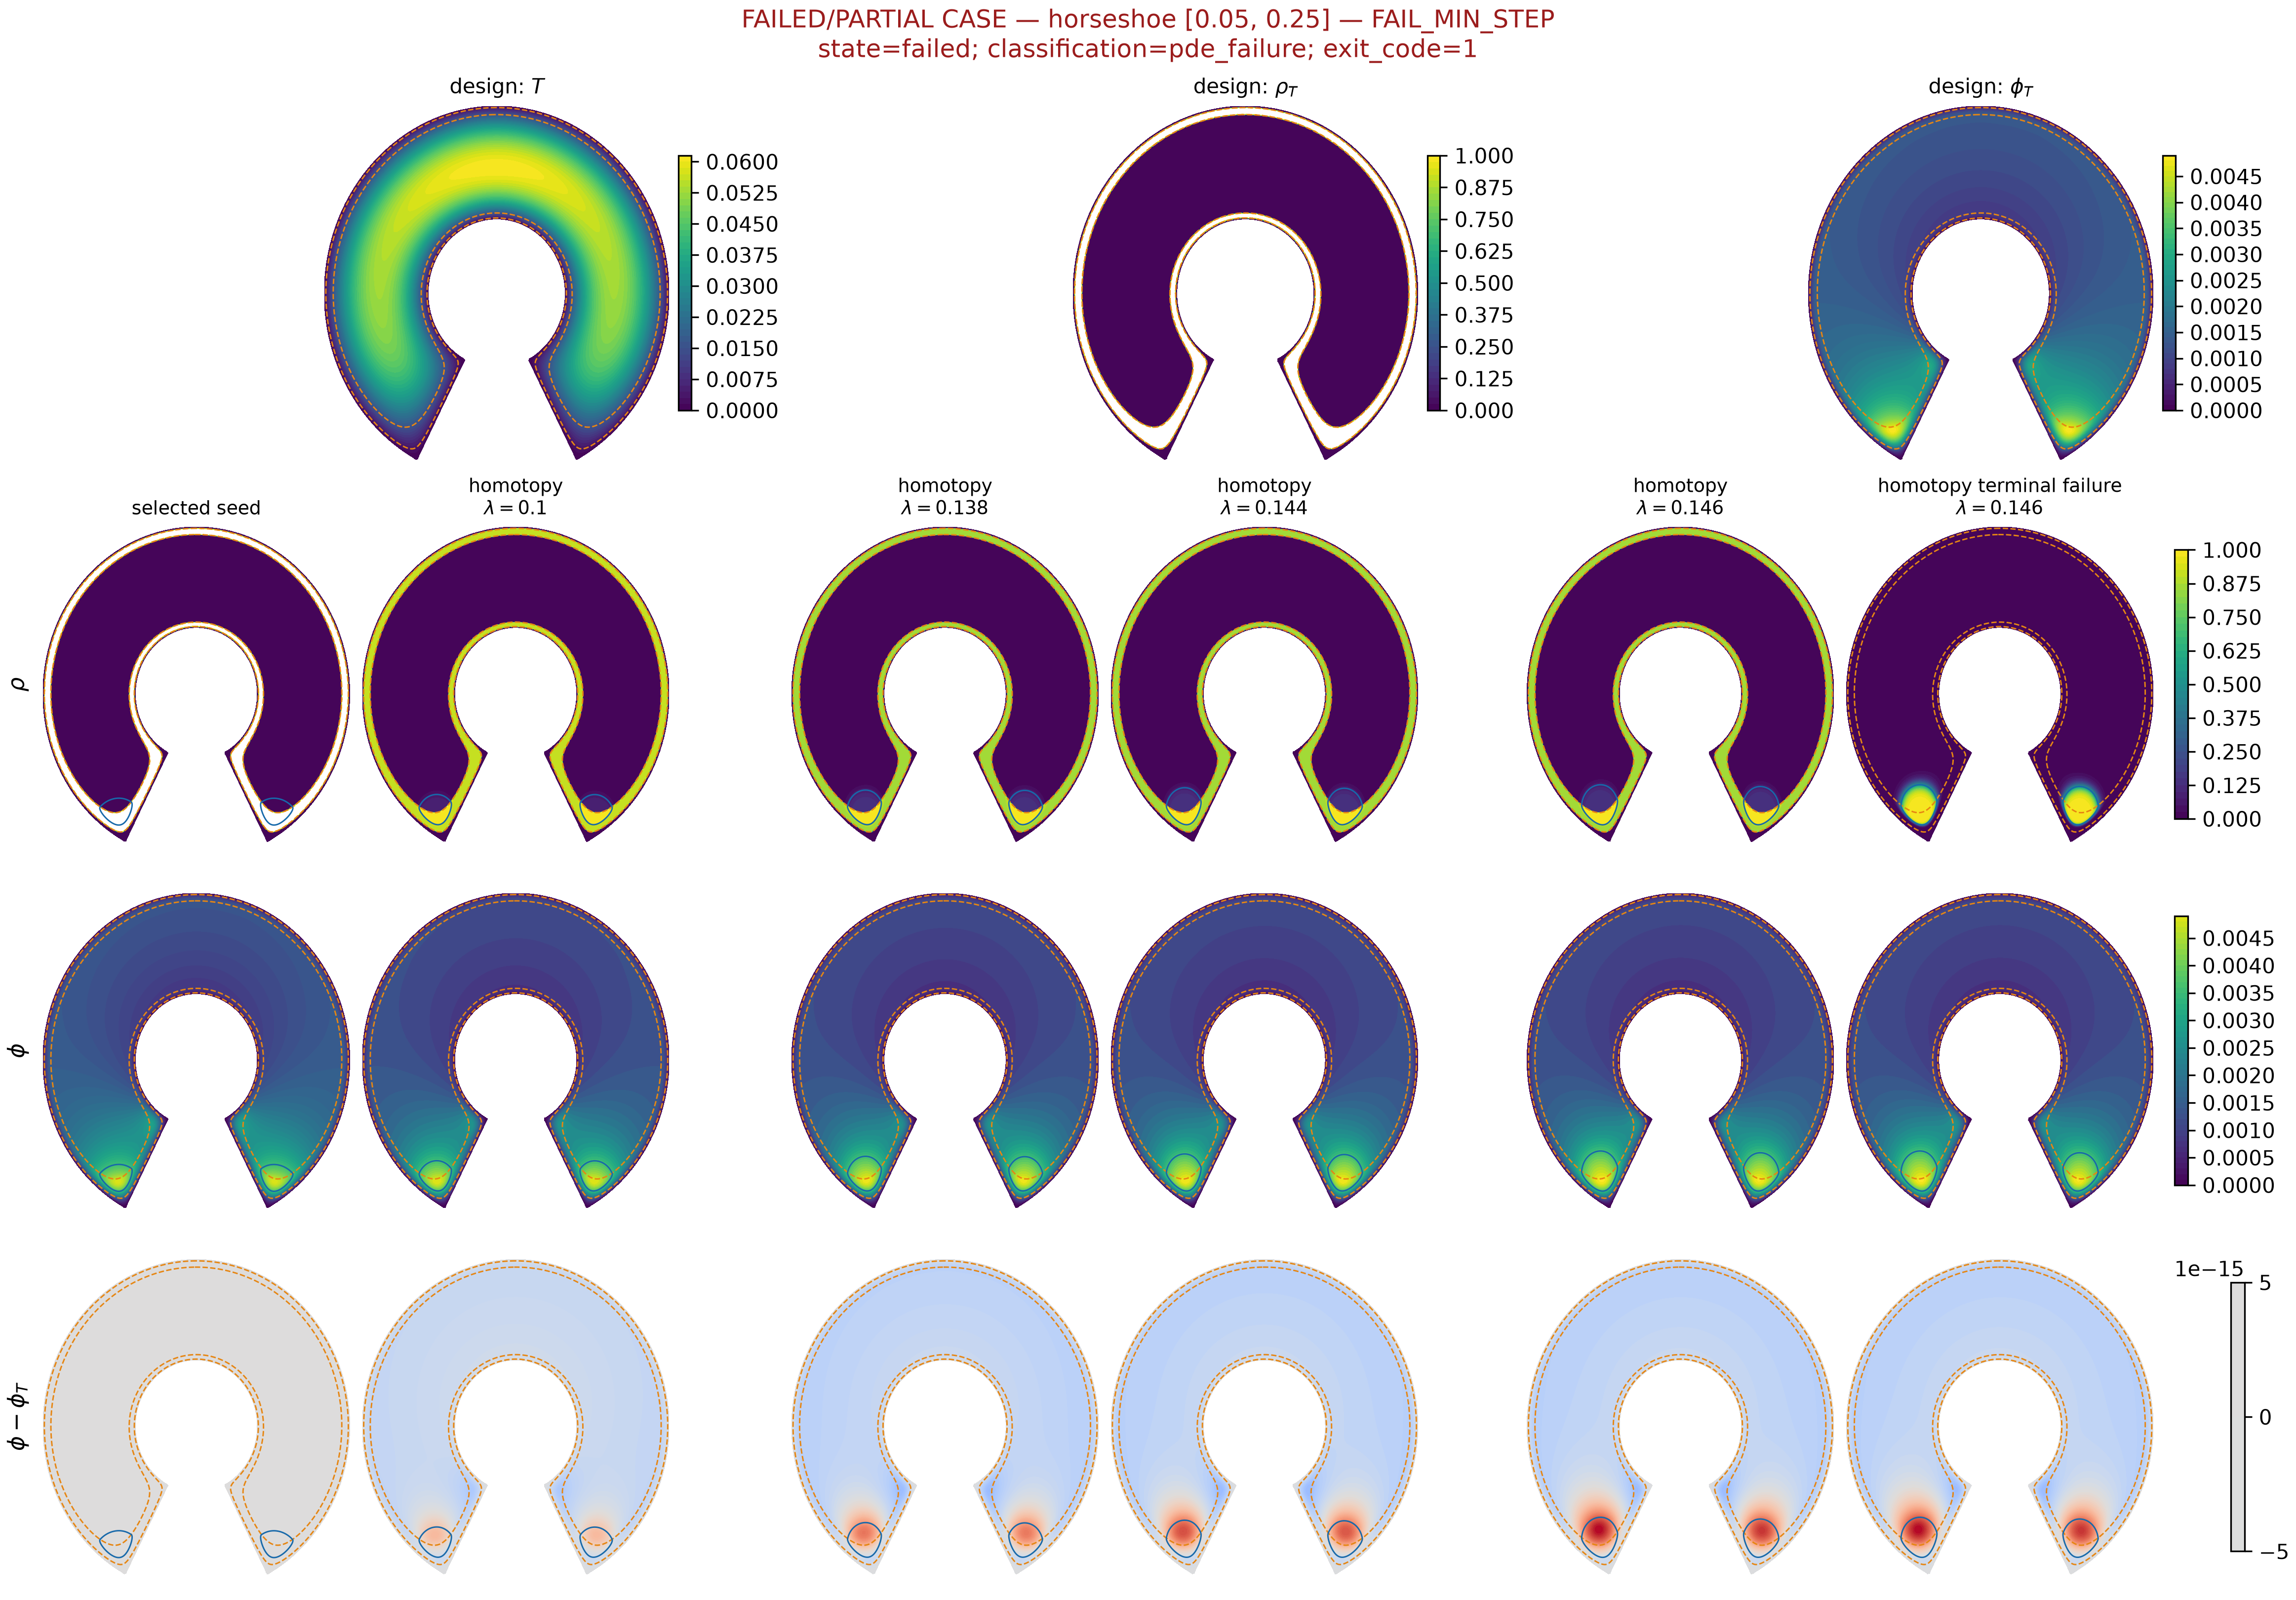
\includegraphics[width=0.88\linewidth]{figures/failed_band_evolution_021_horseshoe_0p05_0p25_trajectory_candidate-horseshoe-7b66eb2dac47.png}
\caption{Supplemental failed/partial trajectory evidence for horseshoe at torsion levels $[0.05,0.25]$ (case trajectory\_candidate-horseshoe-7b66eb2dac47; state=failed; classification=pde\_failure). The case is retained regardless of PDE or geometric success. Orange dashed curves are the fixed target band and blue solid curves are the moving equilibrium band; when state recovery is impossible, the PNG records the reason. Data status: actual.}
\label{fig:failed-storyboard-trajectory-candidate-horseshoe-7b66eb2dac47}
\end{figure}

\clearpage

\begin{figure}[tbp]
\centering
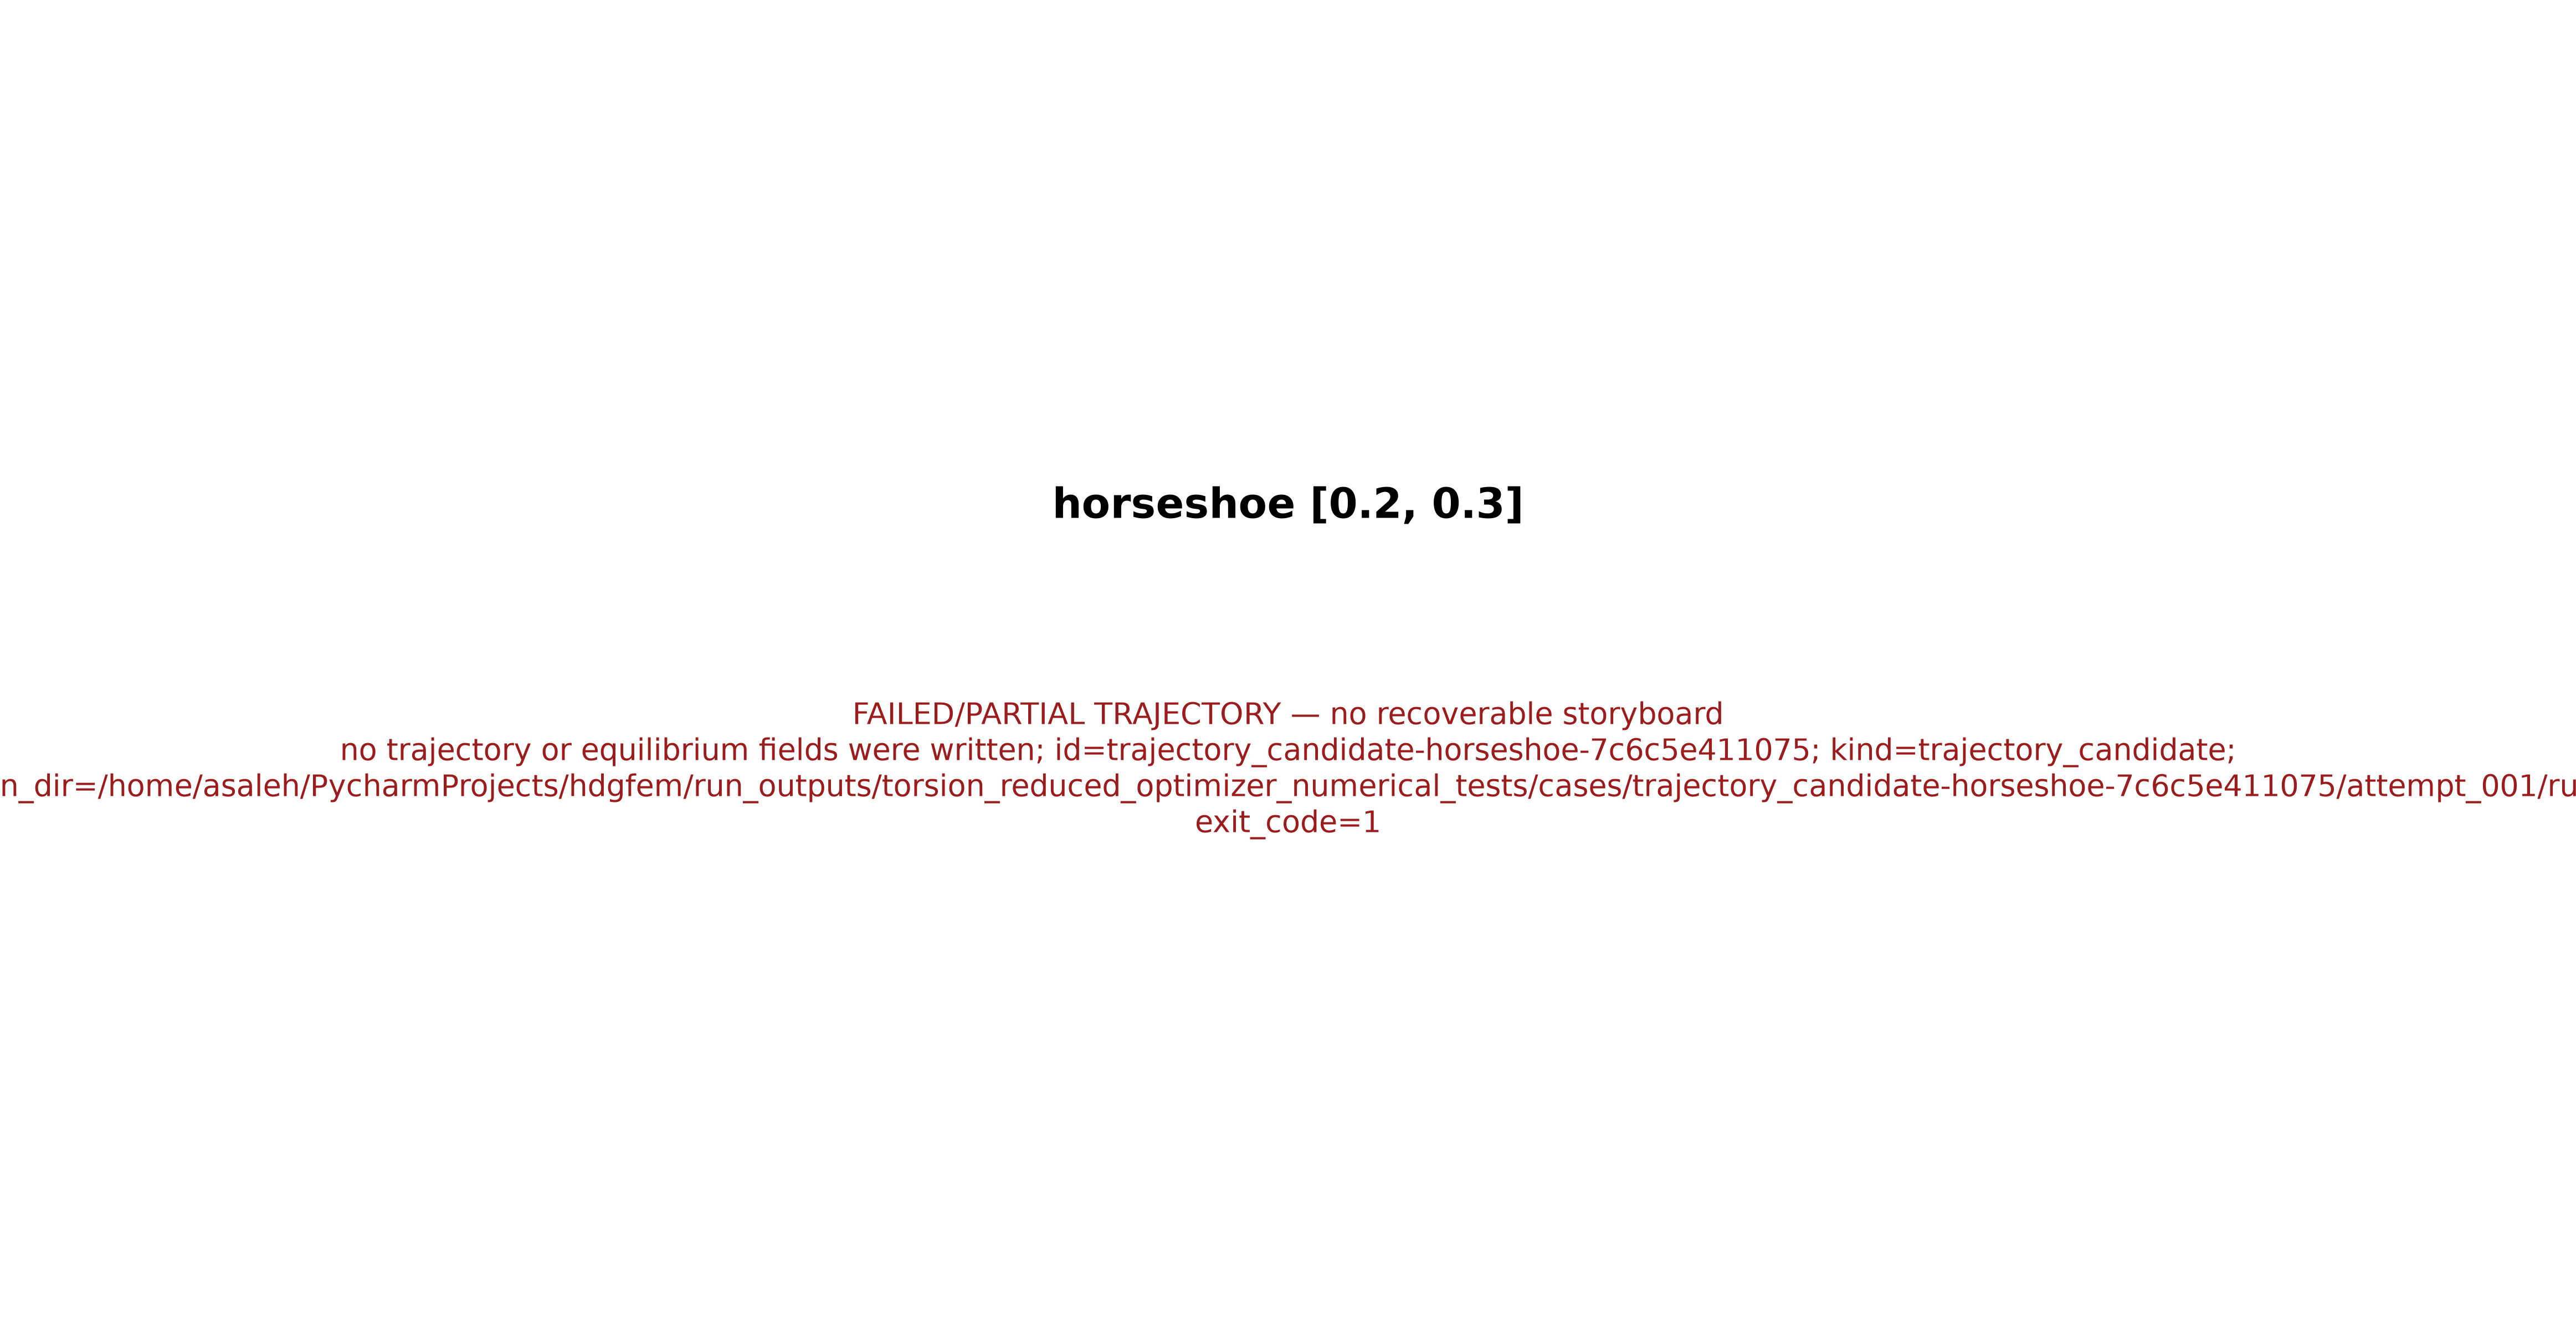
\includegraphics[width=0.88\linewidth]{figures/failed_band_evolution_022_horseshoe_0p2_0p3_trajectory_candidate-horseshoe-7c6c5e411075.png}
\caption{Supplemental failed/partial trajectory evidence for horseshoe at torsion levels $[0.2,0.3]$ (case trajectory\_candidate-horseshoe-7c6c5e411075; state=failed; classification=pde\_failure). The case is retained regardless of PDE or geometric success. Orange dashed curves are the fixed target band and blue solid curves are the moving equilibrium band; when state recovery is impossible, the PNG records the reason. Data status: diagnostic\_only.}
\label{fig:failed-storyboard-trajectory-candidate-horseshoe-7c6c5e411075}
\end{figure}

\begin{figure}[tbp]
\centering
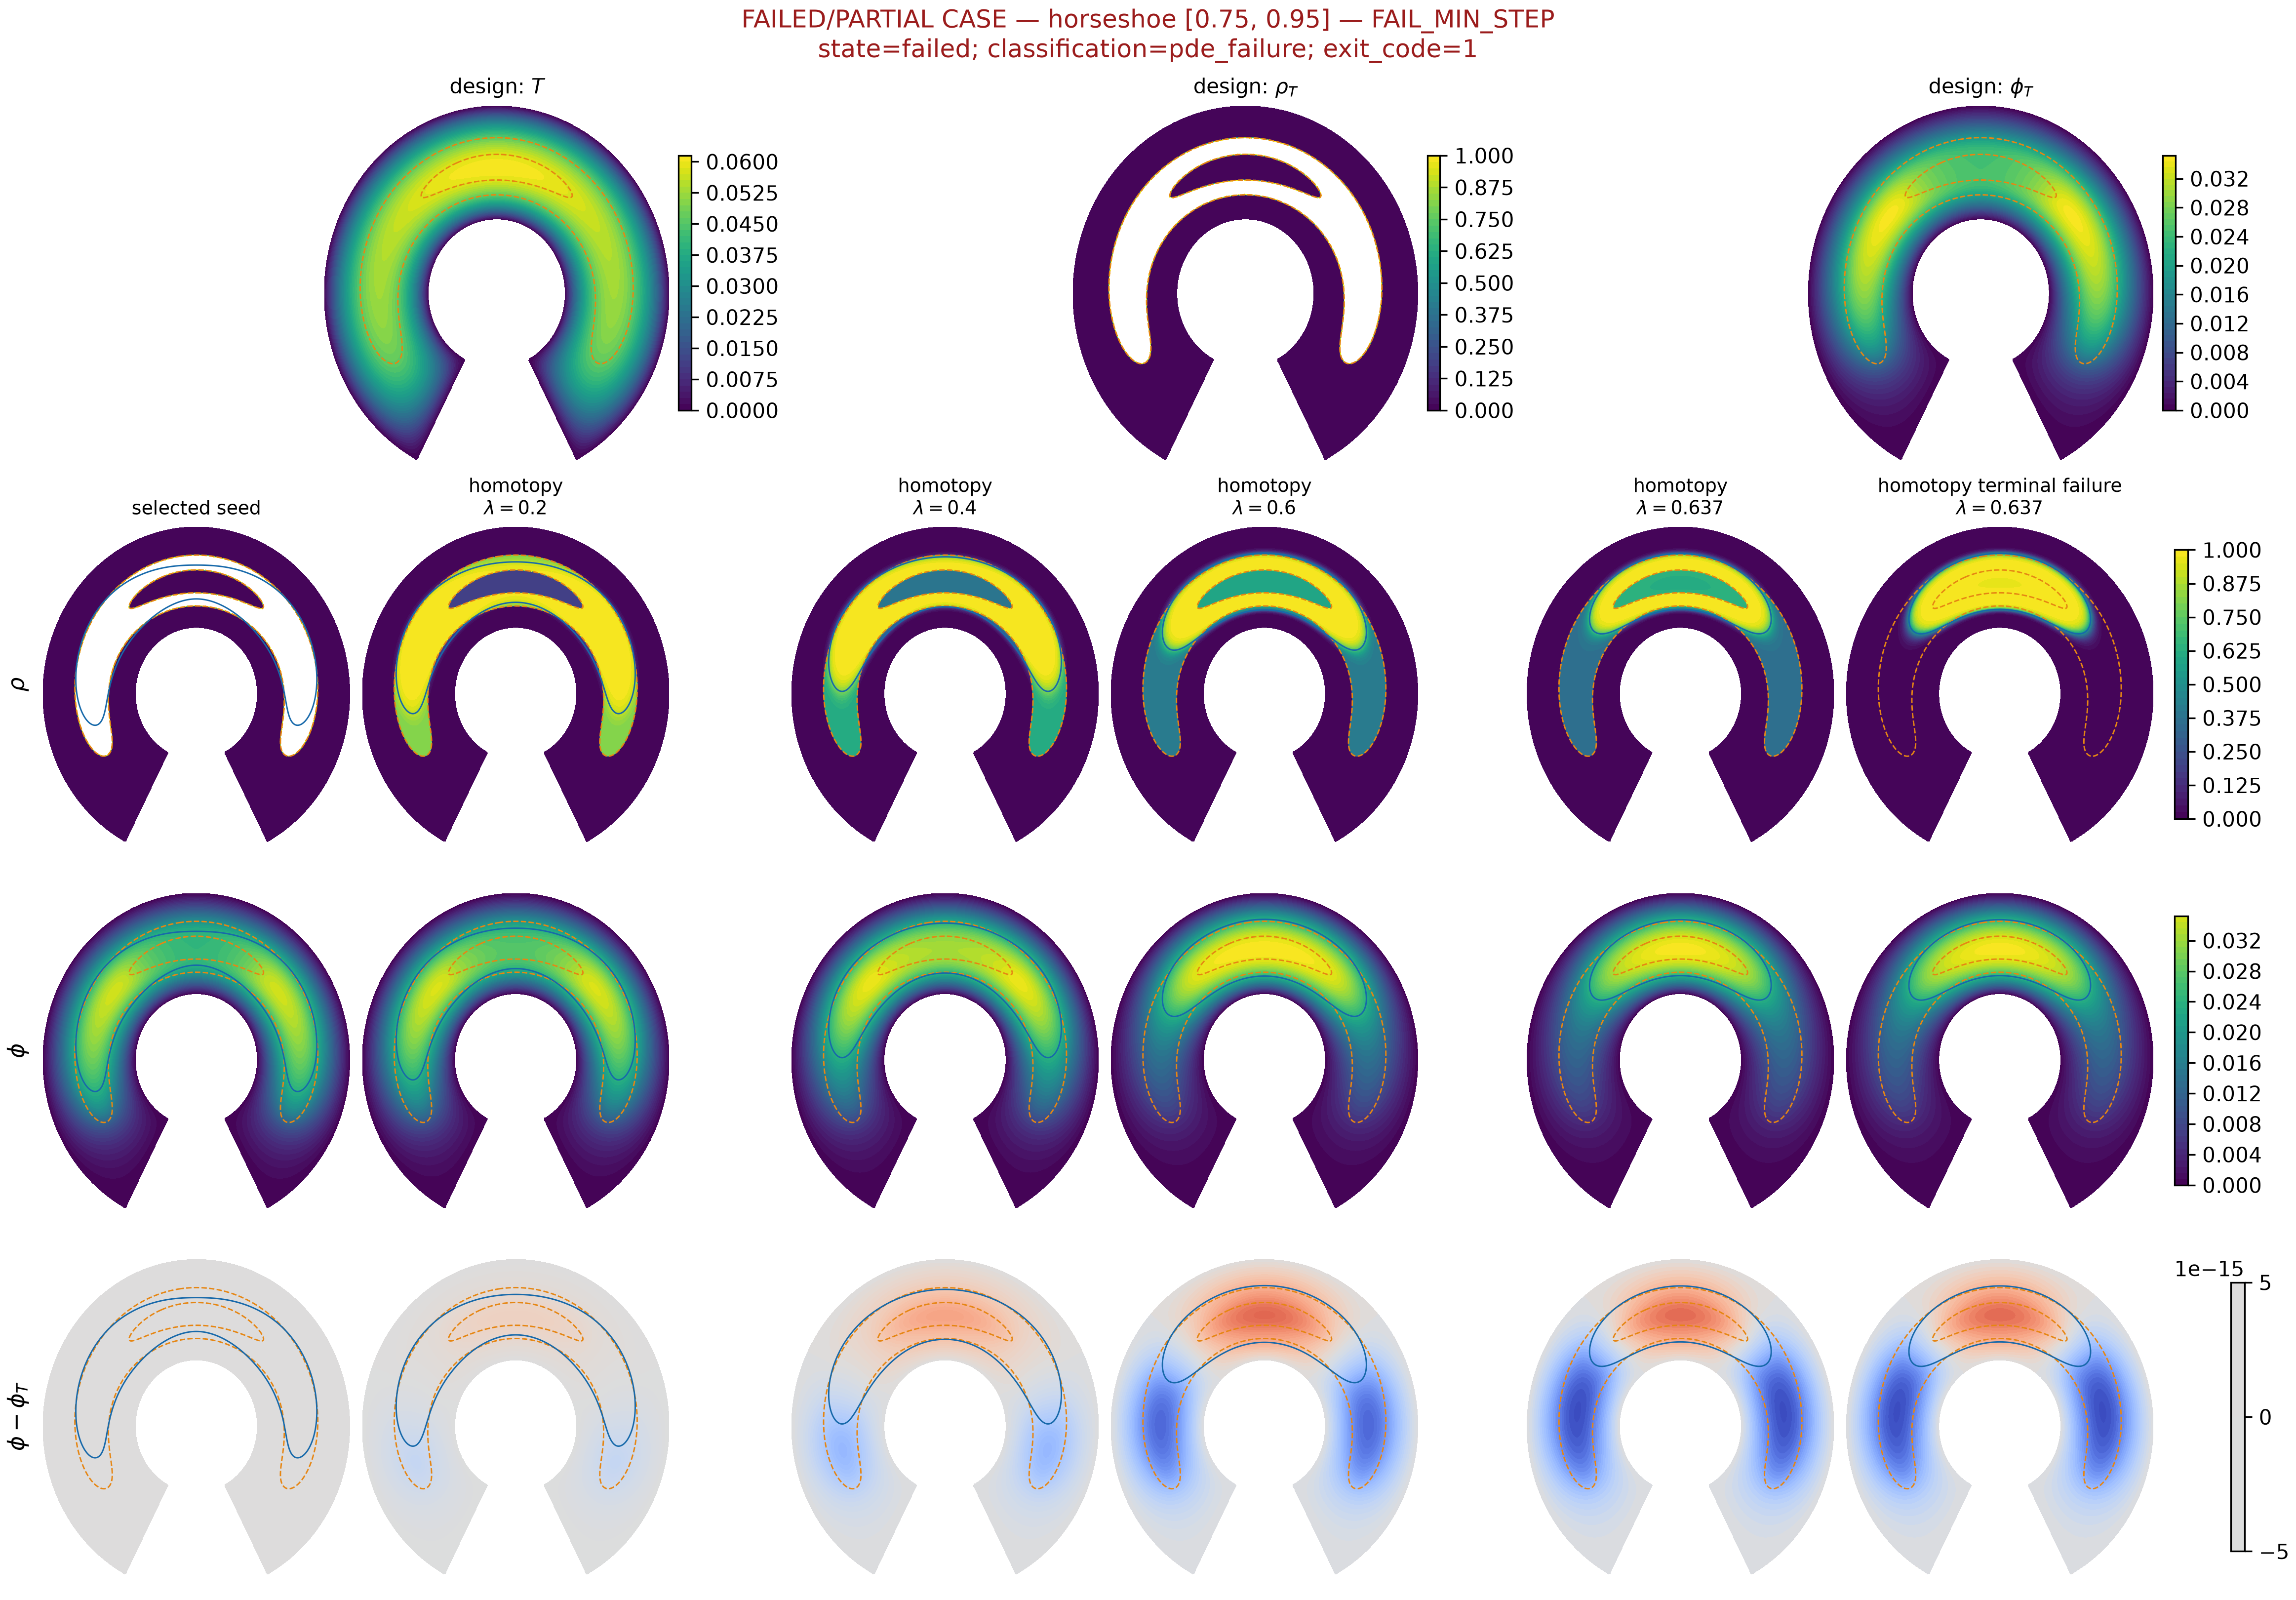
\includegraphics[width=0.88\linewidth]{figures/failed_band_evolution_023_horseshoe_0p75_0p95_trajectory_candidate-horseshoe-961c350b20b3.png}
\caption{Supplemental failed/partial trajectory evidence for horseshoe at torsion levels $[0.75,0.95]$ (case trajectory\_candidate-horseshoe-961c350b20b3; state=failed; classification=pde\_failure). The case is retained regardless of PDE or geometric success. Orange dashed curves are the fixed target band and blue solid curves are the moving equilibrium band; when state recovery is impossible, the PNG records the reason. Data status: actual.}
\label{fig:failed-storyboard-trajectory-candidate-horseshoe-961c350b20b3}
\end{figure}

\begin{figure}[tbp]
\centering
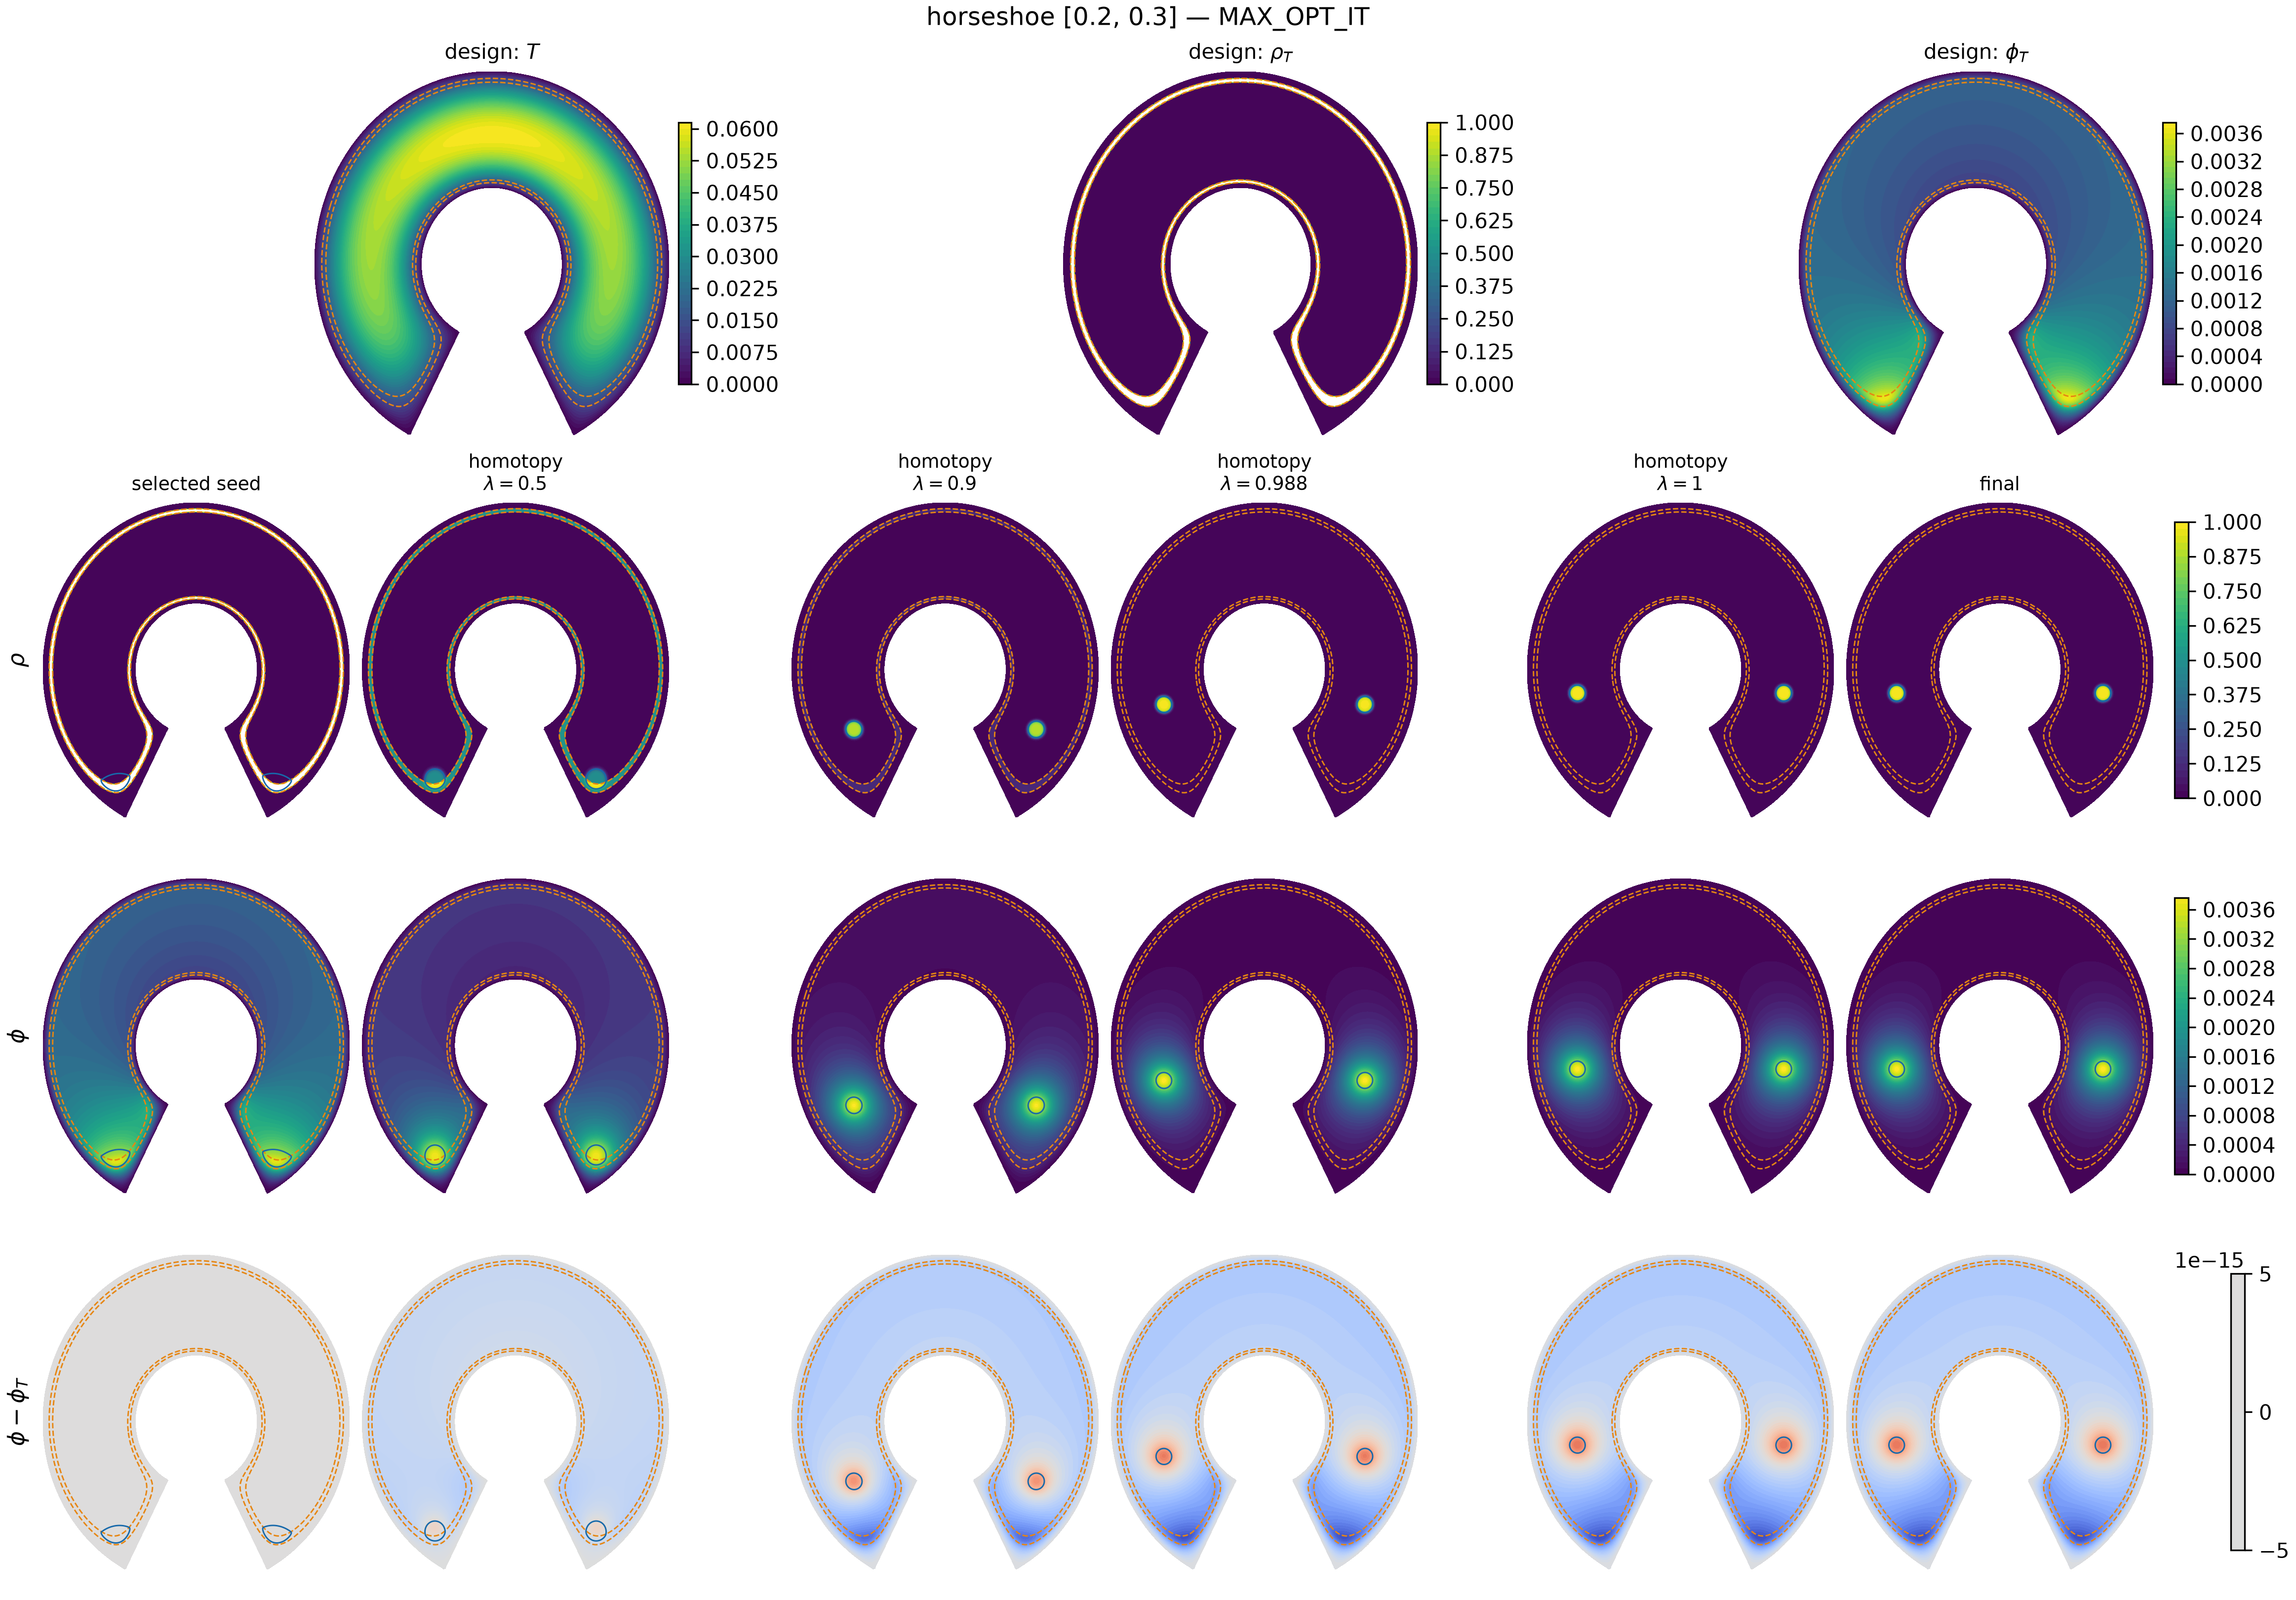
\includegraphics[width=0.88\linewidth]{figures/failed_band_evolution_024_horseshoe_0p2_0p3_trajectory_candidate-horseshoe-9e9172e39927.png}
\caption{Supplemental failed/partial trajectory evidence for horseshoe at torsion levels $[0.2,0.3]$ (case trajectory\_candidate-horseshoe-9e9172e39927; state=completed; classification=geometrically\_unsuccessful\_pde\_converged). The case is retained regardless of PDE or geometric success. Orange dashed curves are the fixed target band and blue solid curves are the moving equilibrium band; when state recovery is impossible, the PNG records the reason. Data status: actual.}
\label{fig:failed-storyboard-trajectory-candidate-horseshoe-9e9172e39927}
\end{figure}

\begin{figure}[tbp]
\centering
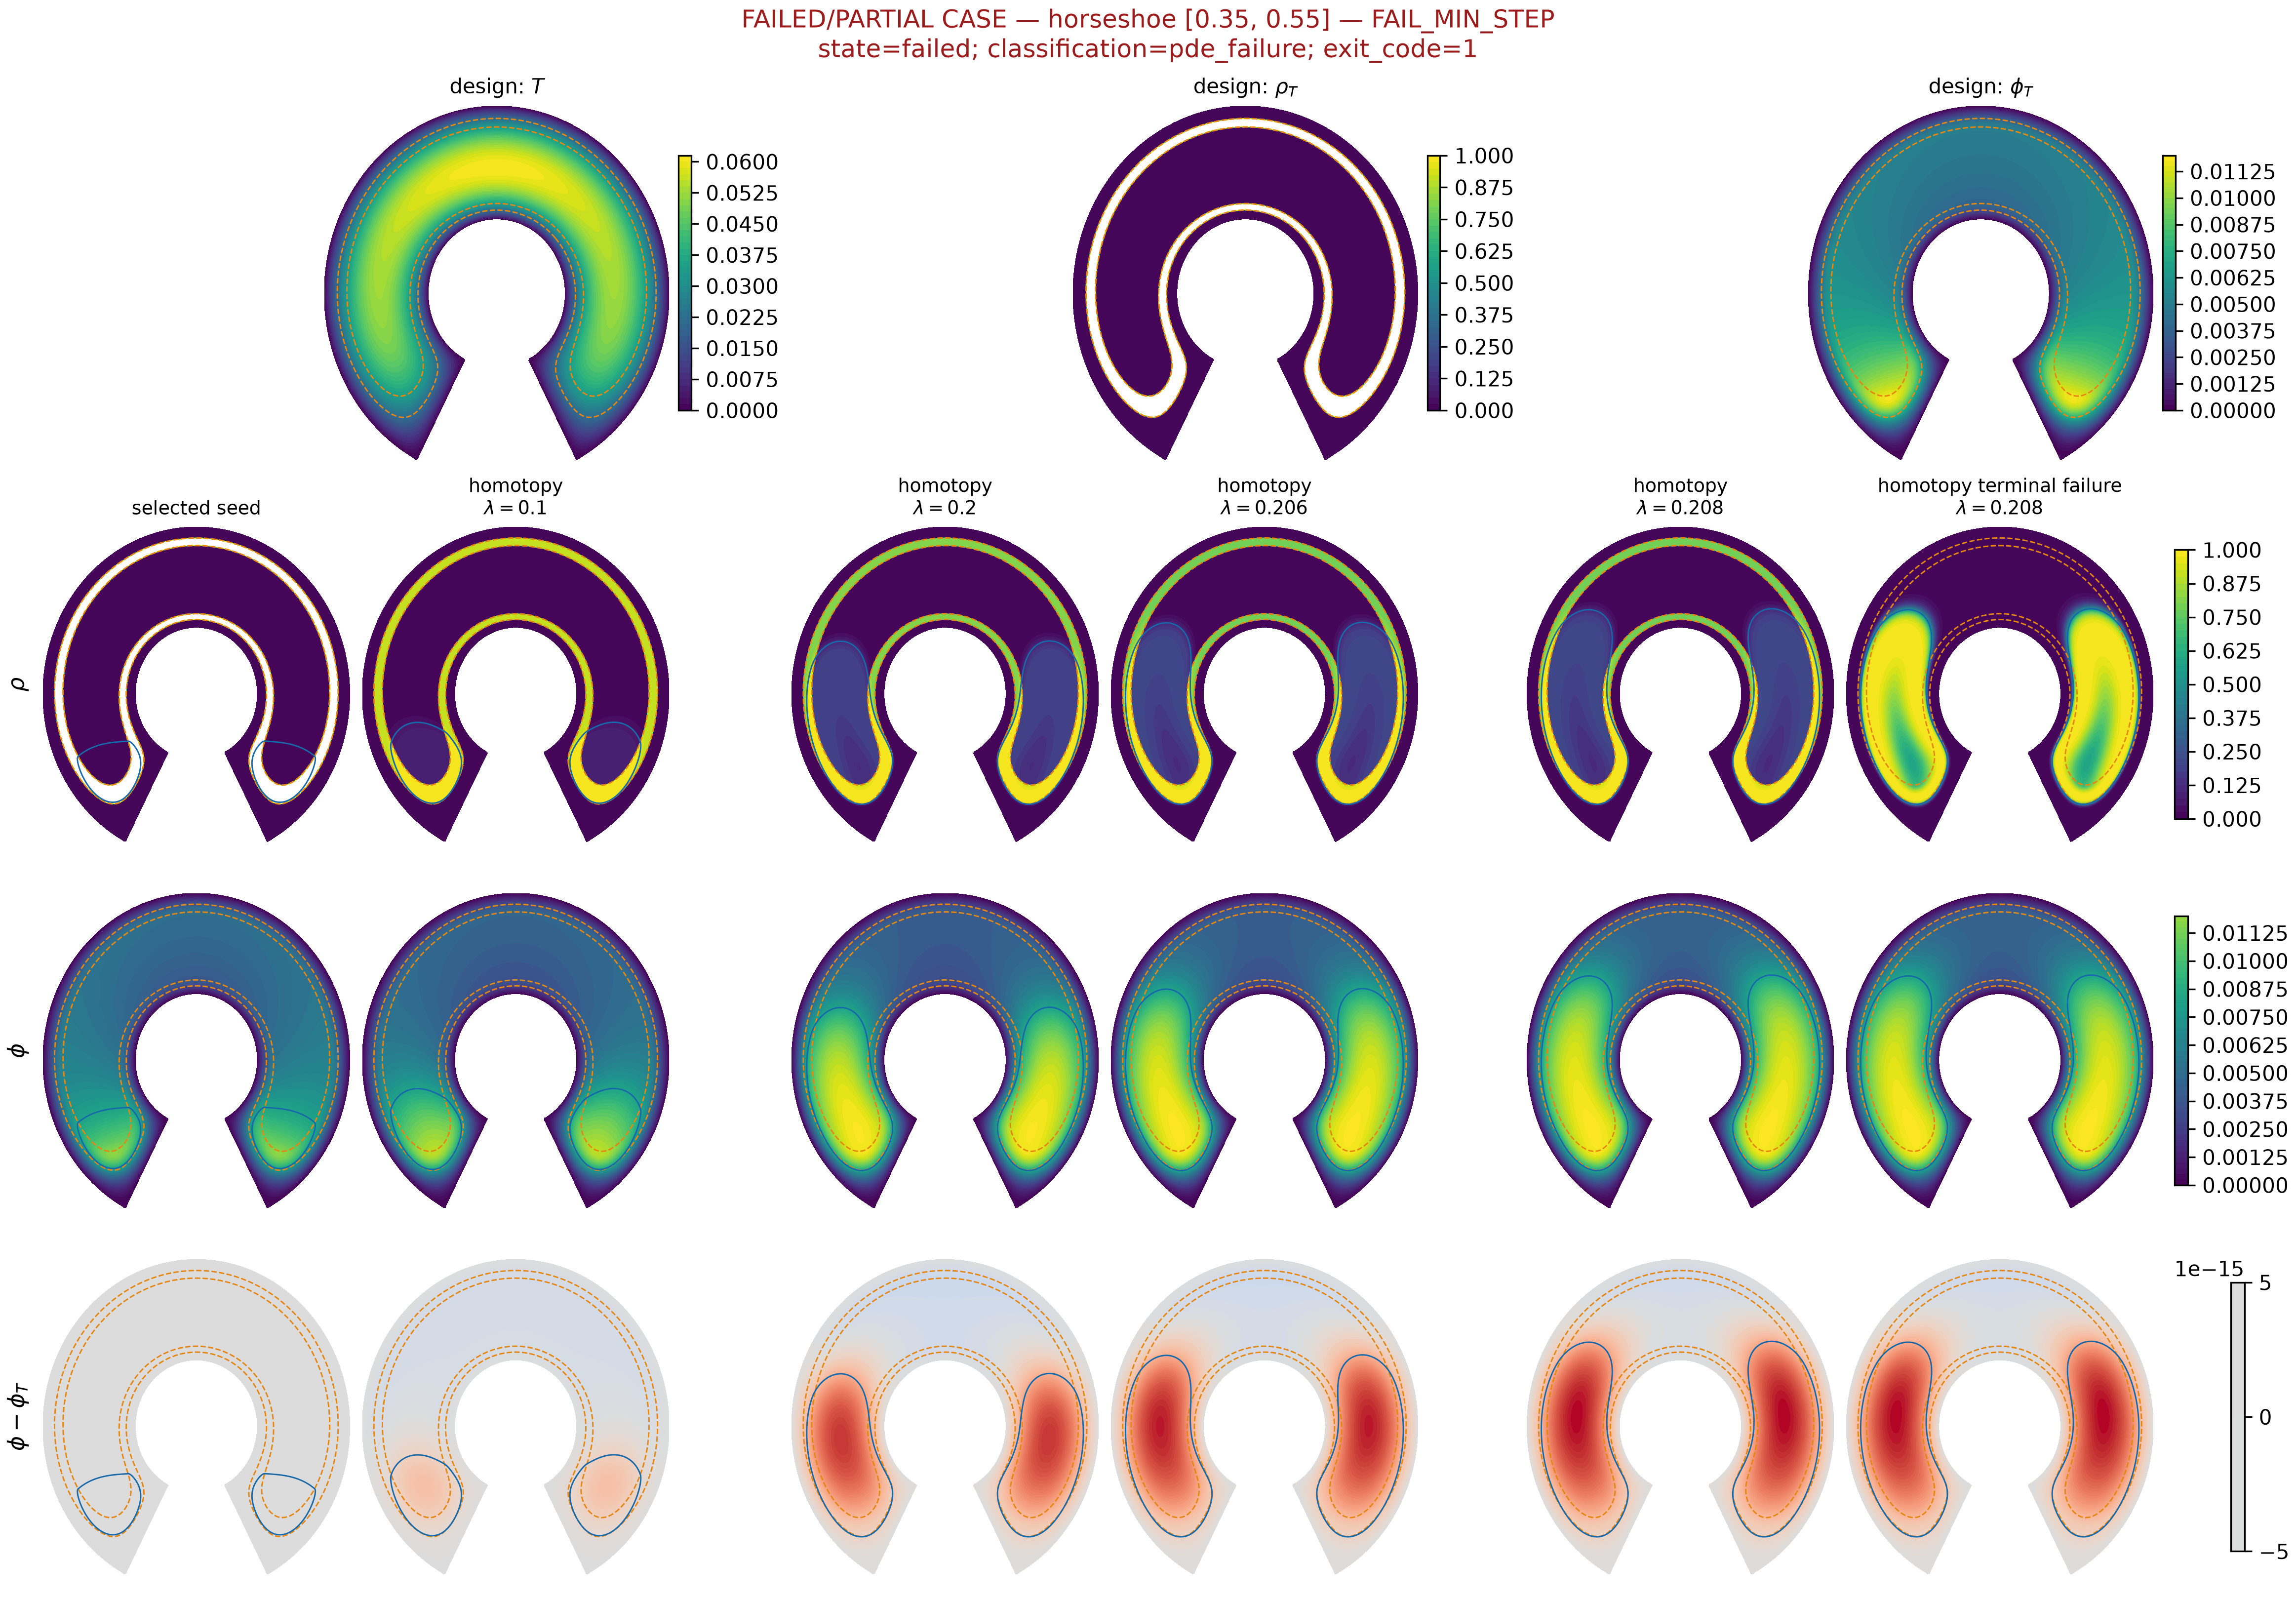
\includegraphics[width=0.88\linewidth]{figures/failed_band_evolution_025_horseshoe_0p35_0p55_trajectory_candidate-horseshoe-a1b396c5c8fc.png}
\caption{Supplemental failed/partial trajectory evidence for horseshoe at torsion levels $[0.35,0.55]$ (case trajectory\_candidate-horseshoe-a1b396c5c8fc; state=failed; classification=pde\_failure). The case is retained regardless of PDE or geometric success. Orange dashed curves are the fixed target band and blue solid curves are the moving equilibrium band; when state recovery is impossible, the PNG records the reason. Data status: actual.}
\label{fig:failed-storyboard-trajectory-candidate-horseshoe-a1b396c5c8fc}
\end{figure}

\begin{figure}[tbp]
\centering
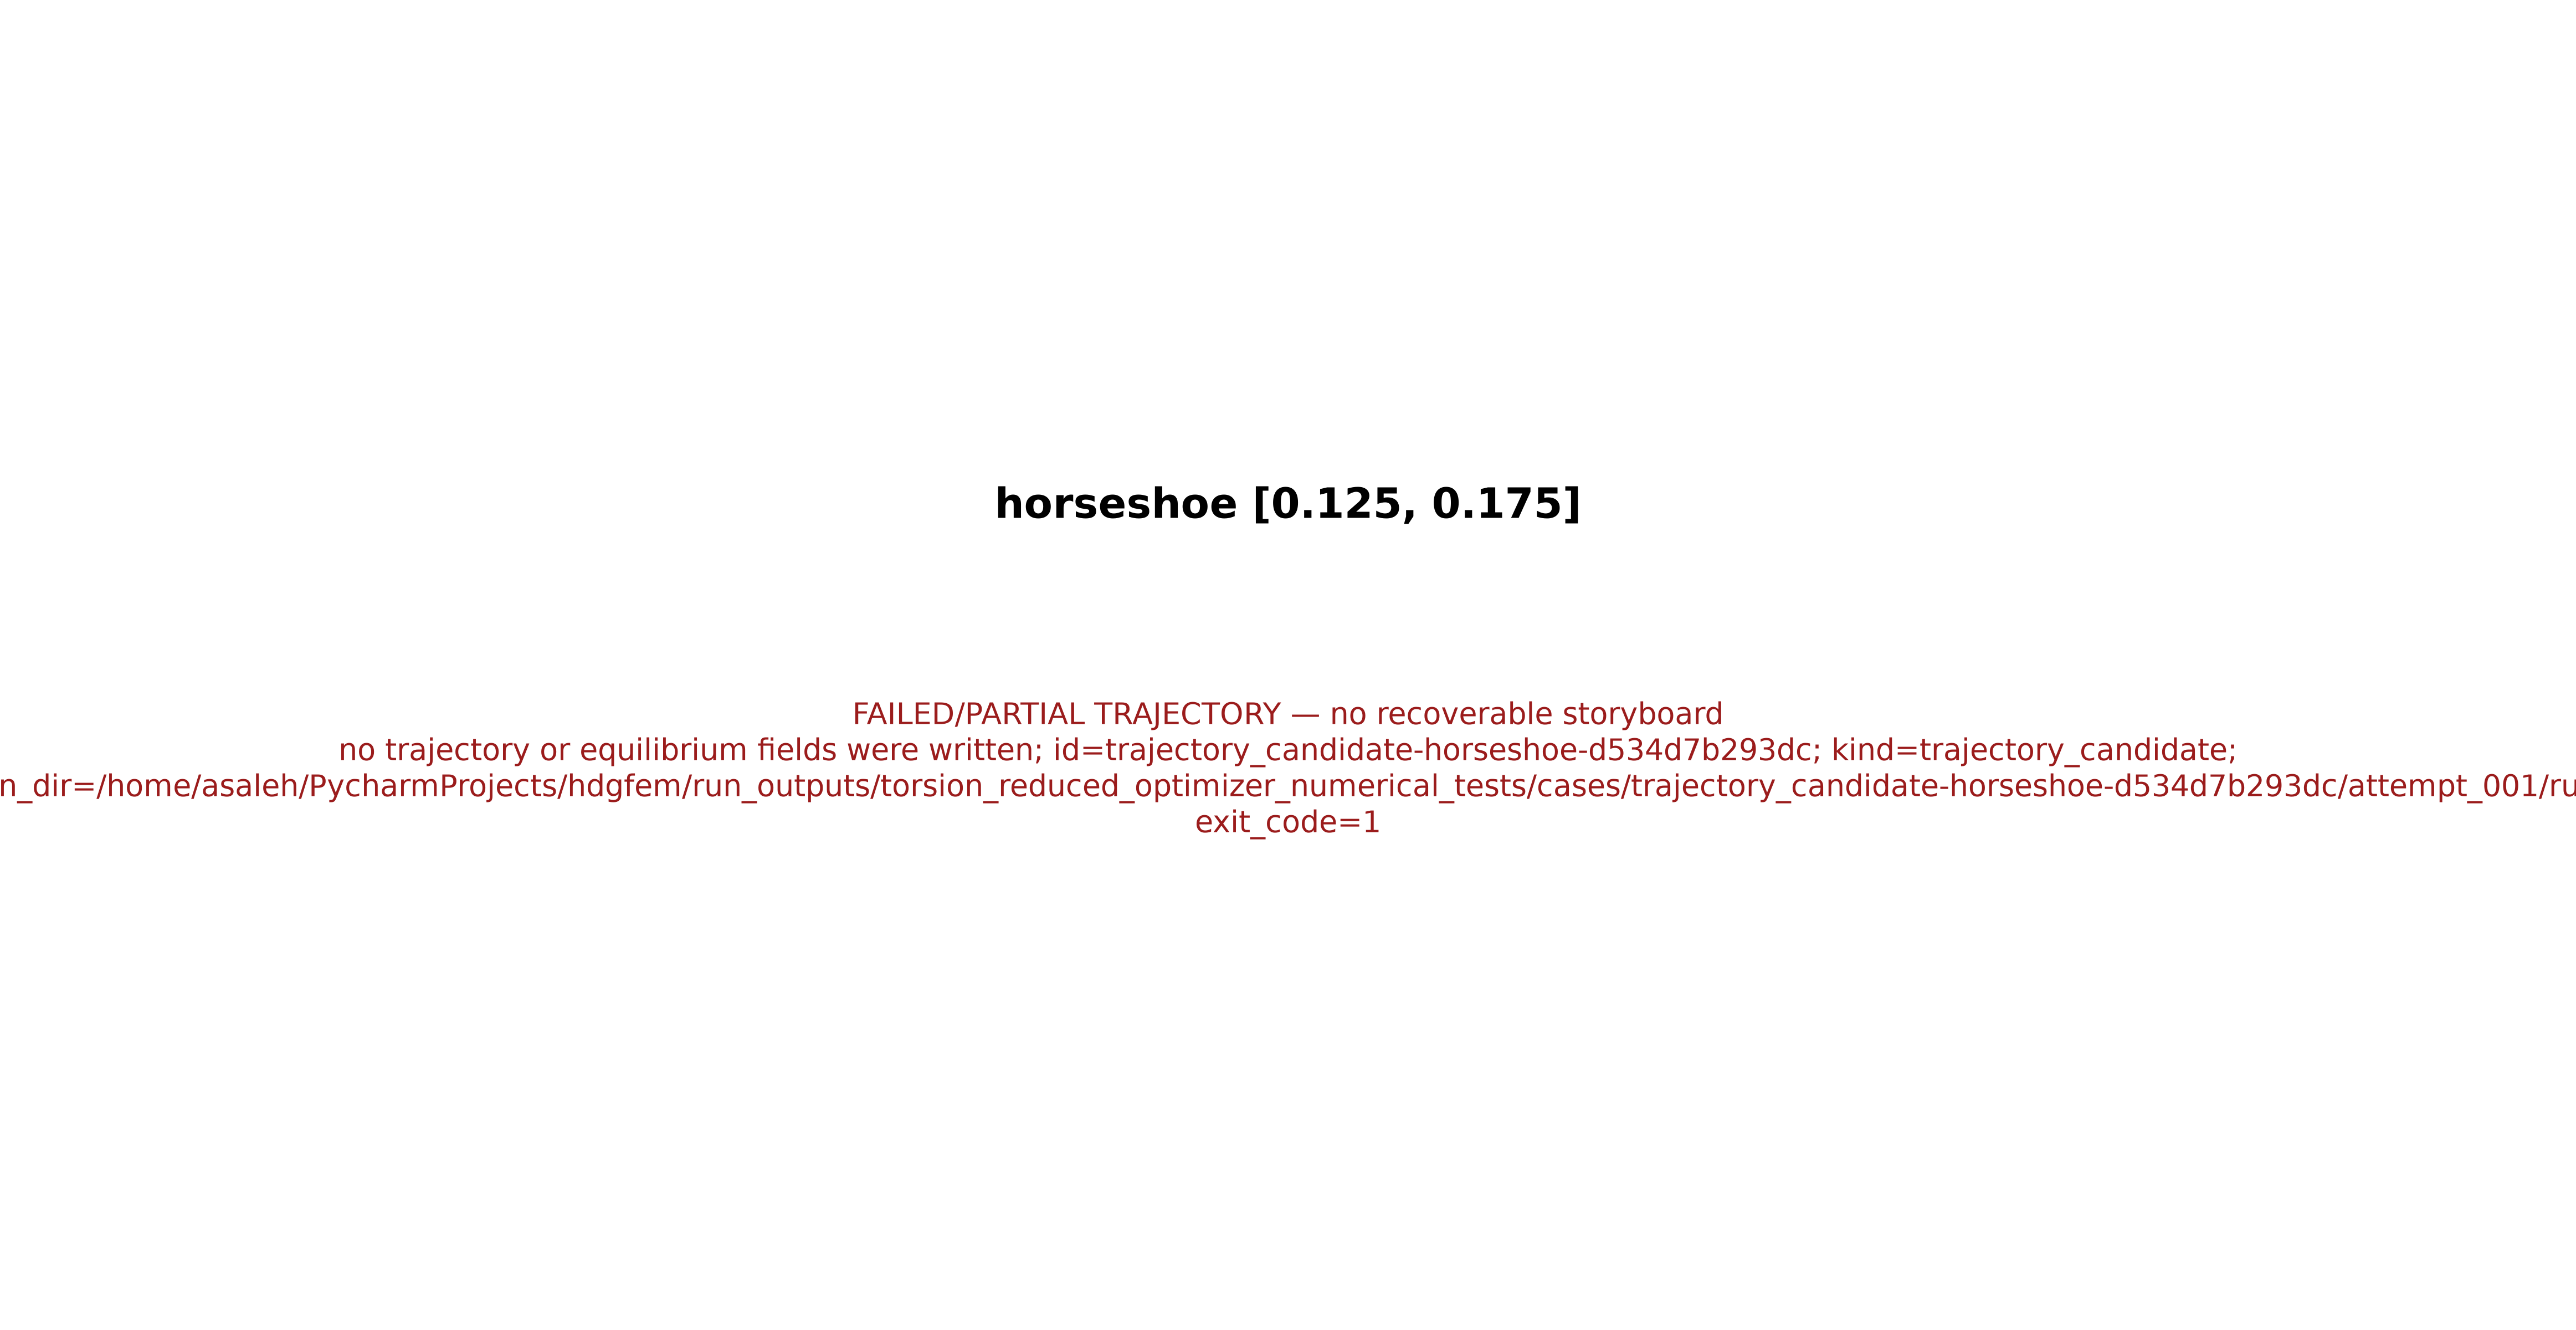
\includegraphics[width=0.88\linewidth]{figures/failed_band_evolution_026_horseshoe_0p125_0p175_trajectory_candidate-horseshoe-d534d7b293dc.png}
\caption{Supplemental failed/partial trajectory evidence for horseshoe at torsion levels $[0.125,0.175]$ (case trajectory\_candidate-horseshoe-d534d7b293dc; state=failed; classification=pde\_failure). The case is retained regardless of PDE or geometric success. Orange dashed curves are the fixed target band and blue solid curves are the moving equilibrium band; when state recovery is impossible, the PNG records the reason. Data status: diagnostic\_only.}
\label{fig:failed-storyboard-trajectory-candidate-horseshoe-d534d7b293dc}
\end{figure}

\begin{figure}[tbp]
\centering
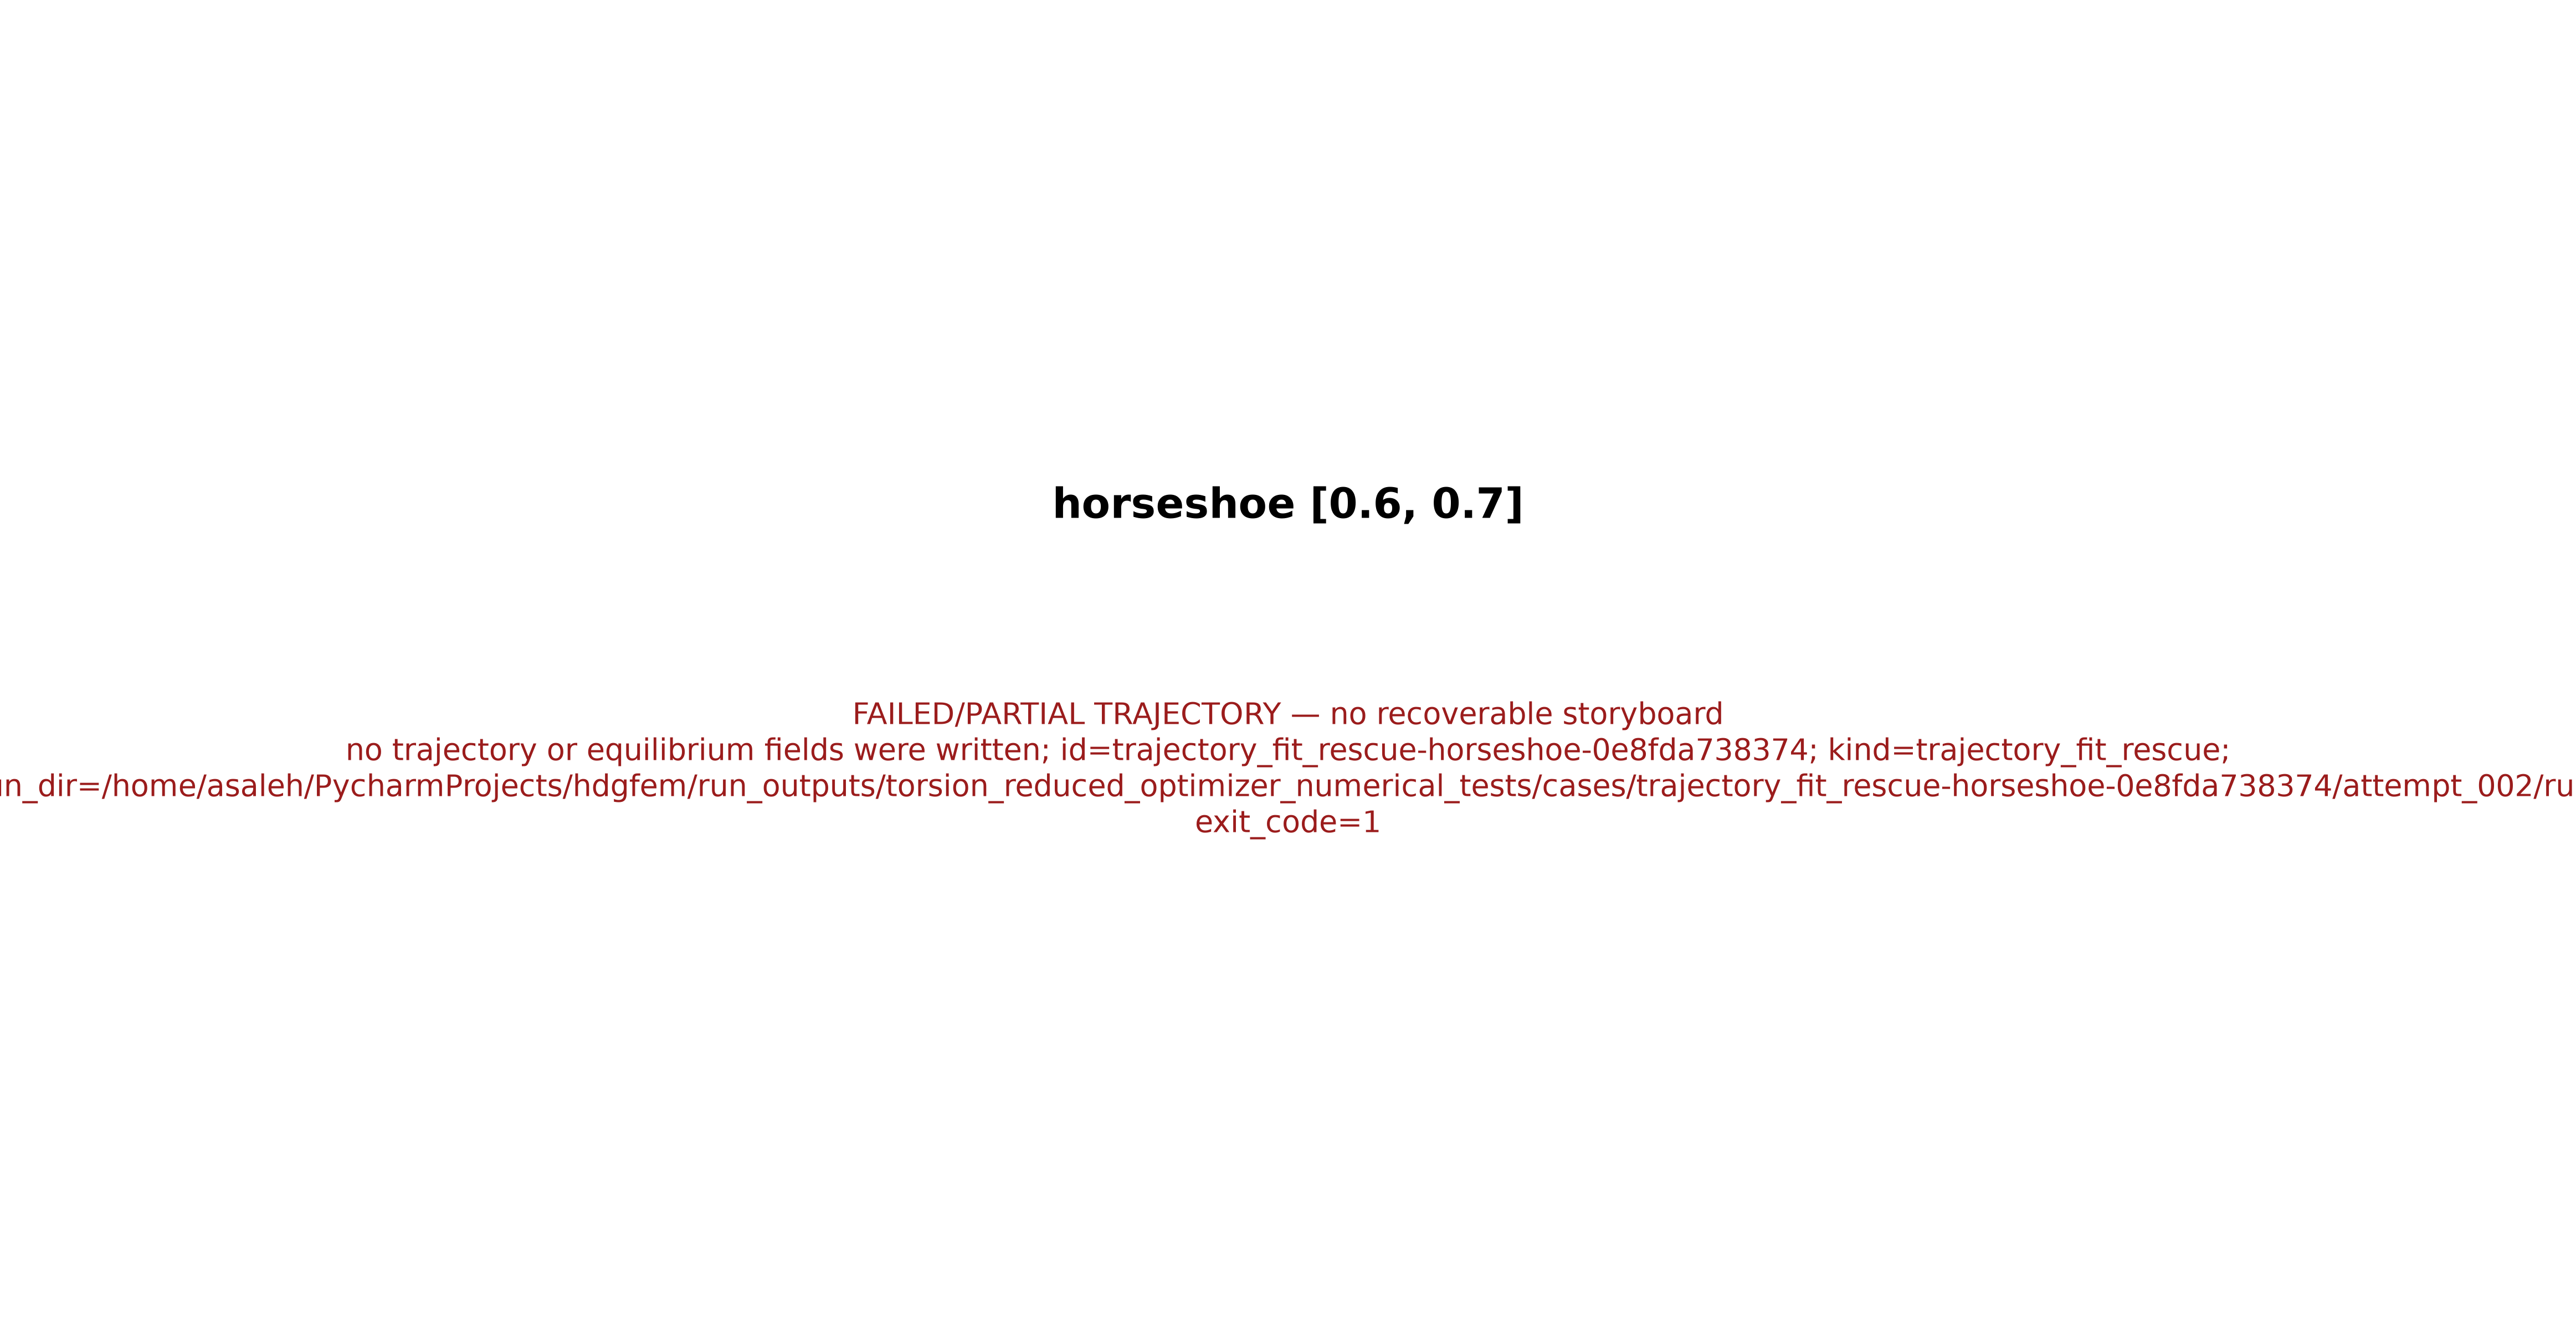
\includegraphics[width=0.88\linewidth]{figures/failed_band_evolution_027_horseshoe_0p6_0p7_trajectory_fit_rescue-horseshoe-0e8fda738374.png}
\caption{Supplemental failed/partial trajectory evidence for horseshoe at torsion levels $[0.6,0.7]$ (case trajectory\_fit\_rescue-horseshoe-0e8fda738374; state=failed; classification=pde\_failure). The case is retained regardless of PDE or geometric success. Orange dashed curves are the fixed target band and blue solid curves are the moving equilibrium band; when state recovery is impossible, the PNG records the reason. Data status: diagnostic\_only.}
\label{fig:failed-storyboard-trajectory-fit-rescue-horseshoe-0e8fda738374}
\end{figure}

\begin{figure}[tbp]
\centering
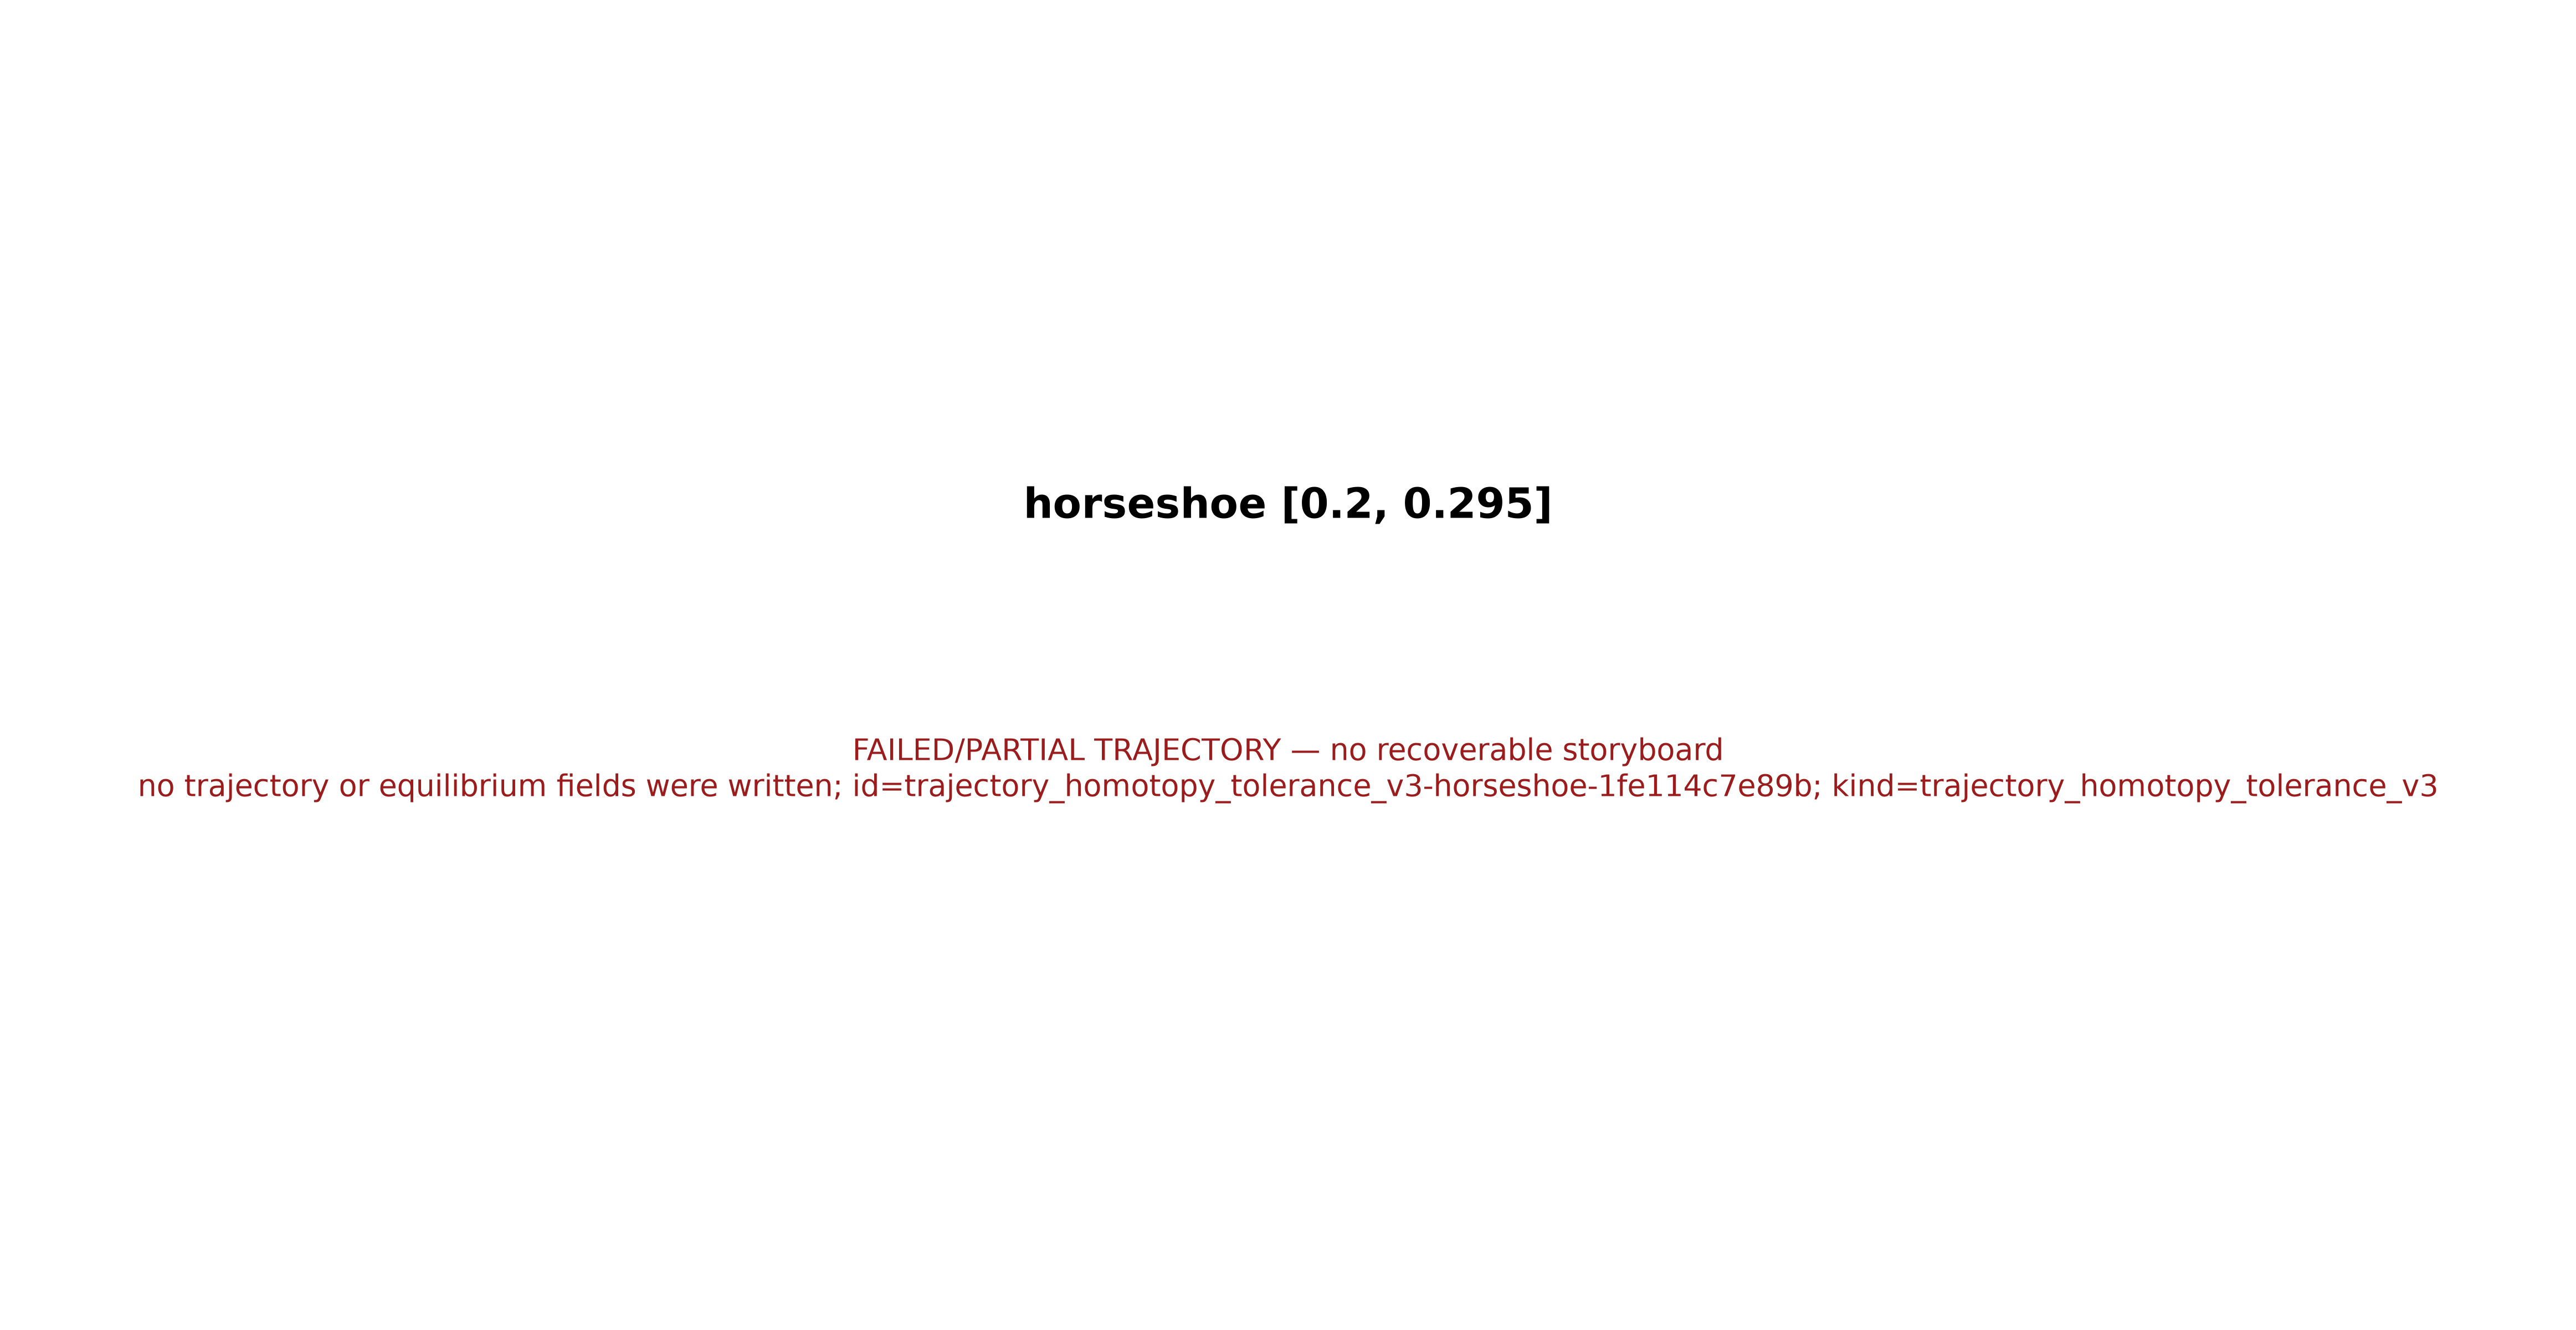
\includegraphics[width=0.88\linewidth]{figures/failed_band_evolution_028_horseshoe_0p2_0p295_trajectory_homotopy_tolerance_v3-horseshoe-1fe114c7e89b.png}
\caption{Supplemental failed/partial trajectory evidence for horseshoe at torsion levels $[0.2,0.295]$ (case trajectory\_homotopy\_tolerance\_v3-horseshoe-1fe114c7e89b; state=planned; classification=incomplete). The case is retained regardless of PDE or geometric success. Orange dashed curves are the fixed target band and blue solid curves are the moving equilibrium band; when state recovery is impossible, the PNG records the reason. Data status: diagnostic\_only.}
\label{fig:failed-storyboard-trajectory-homotopy-tolerance-v3-horseshoe-1fe114c7e89b}
\end{figure}

\begin{figure}[tbp]
\centering
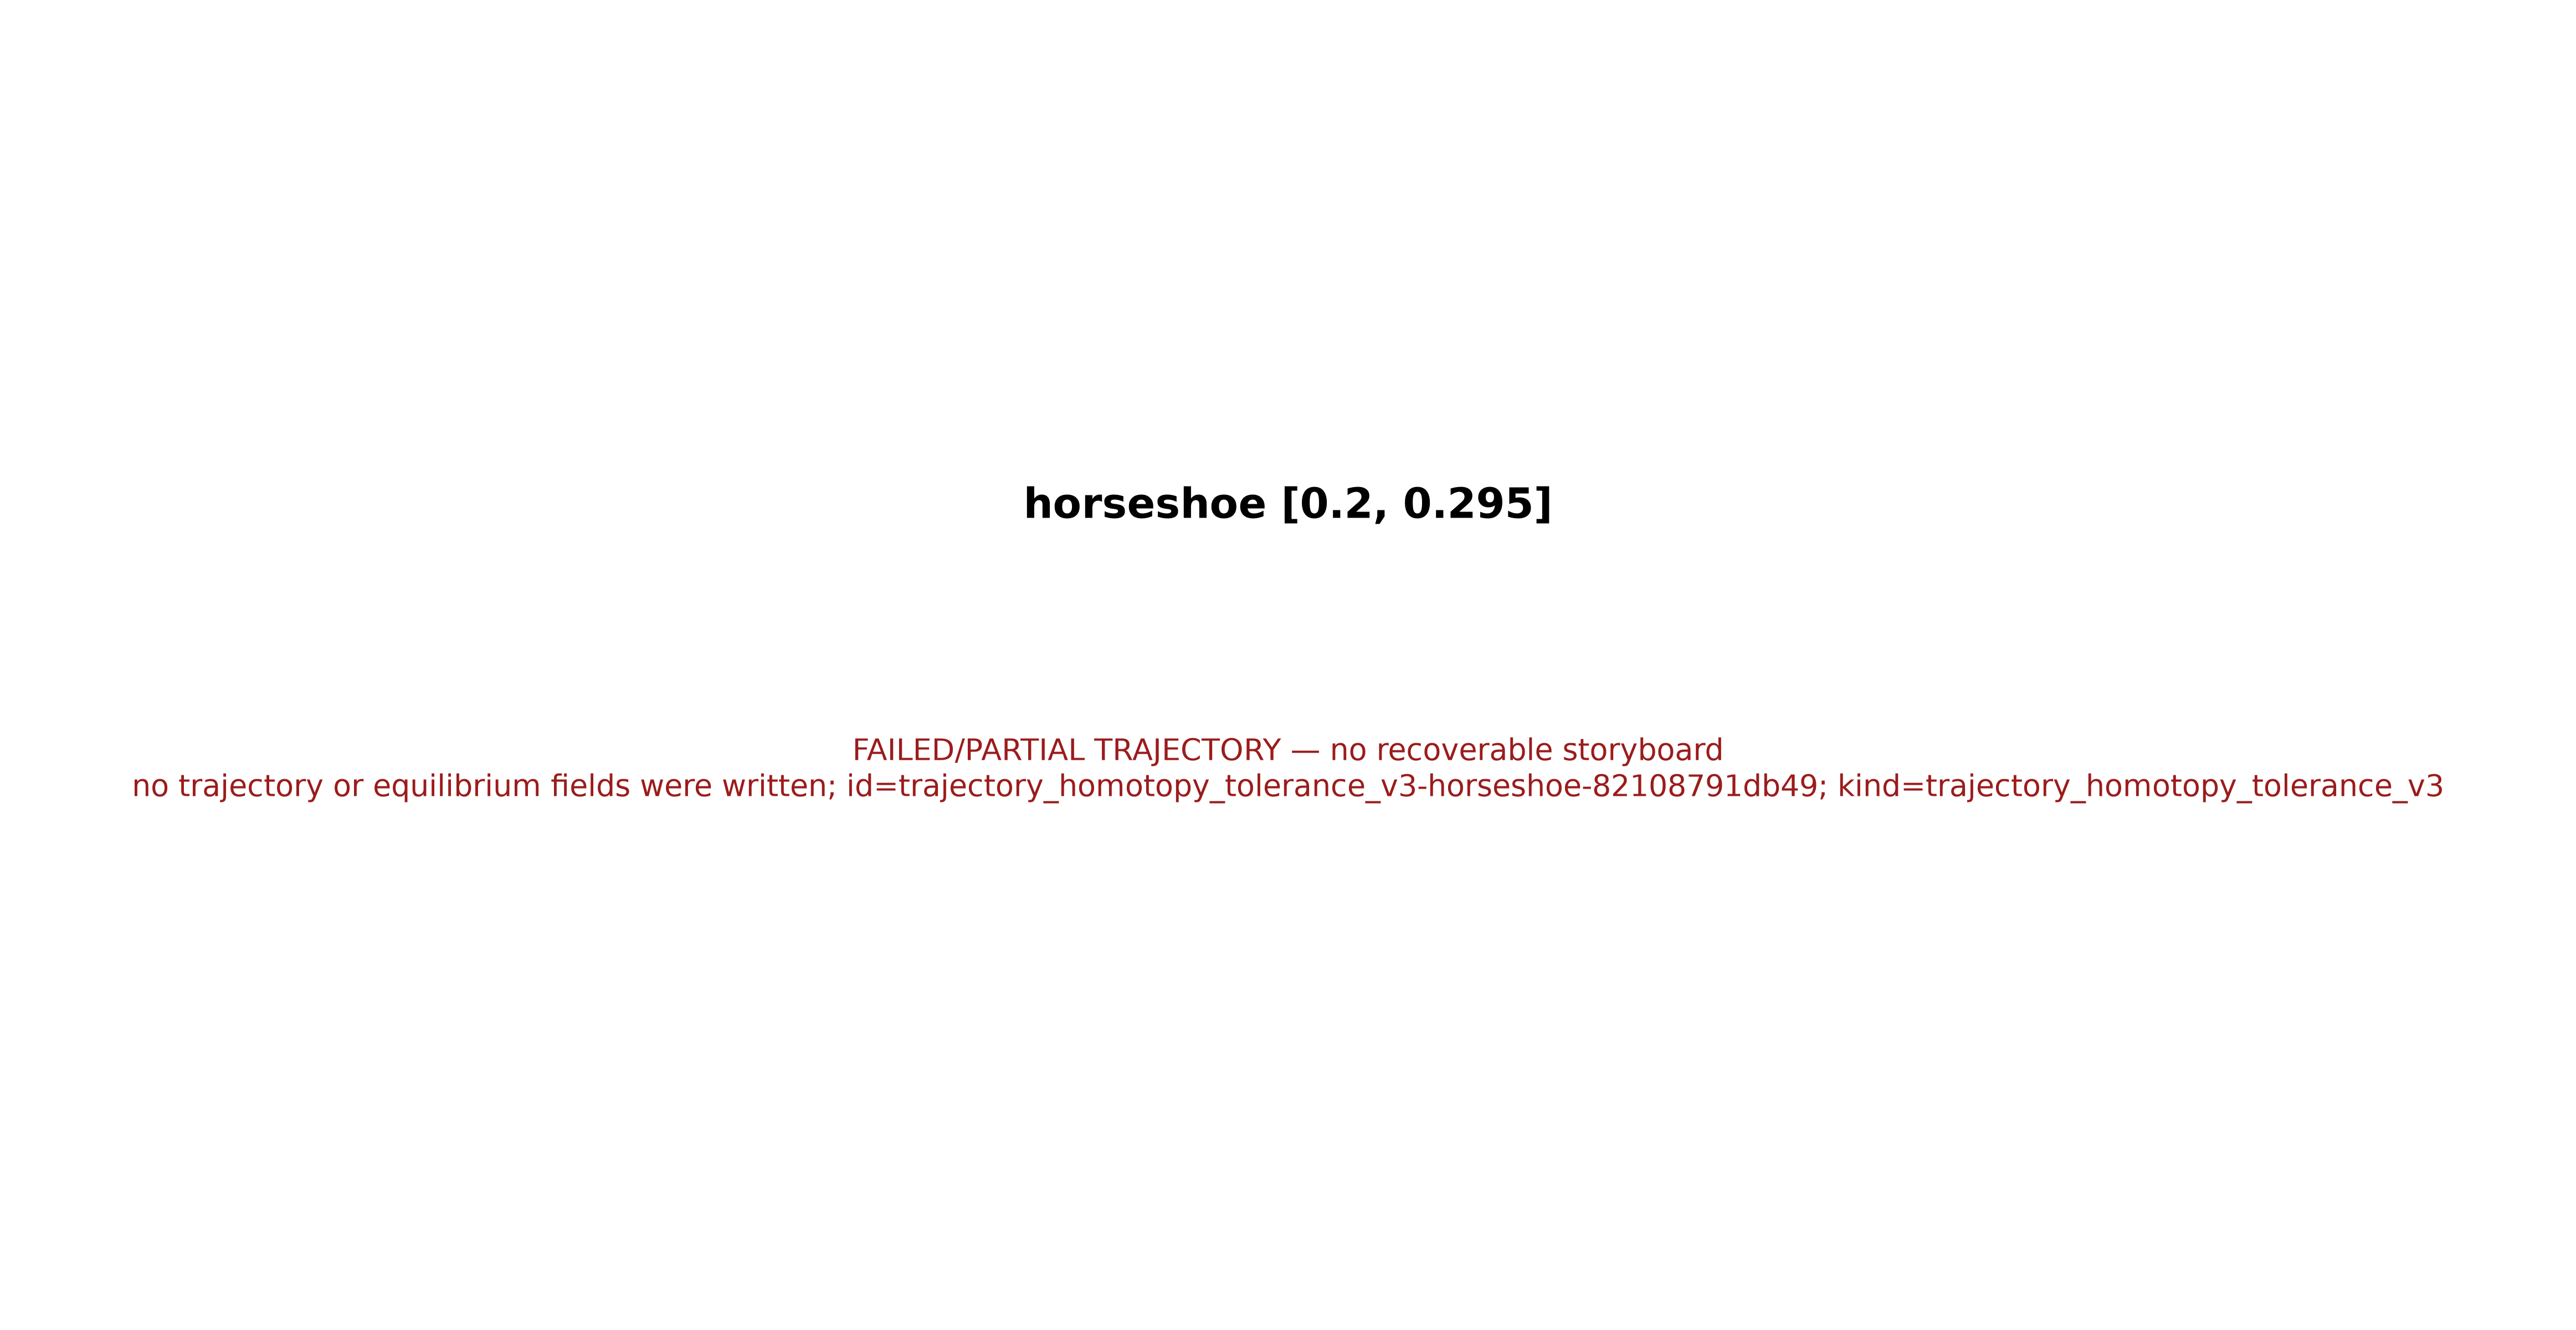
\includegraphics[width=0.88\linewidth]{figures/failed_band_evolution_029_horseshoe_0p2_0p295_trajectory_homotopy_tolerance_v3-horseshoe-82108791db49.png}
\caption{Supplemental failed/partial trajectory evidence for horseshoe at torsion levels $[0.2,0.295]$ (case trajectory\_homotopy\_tolerance\_v3-horseshoe-82108791db49; state=planned; classification=incomplete). The case is retained regardless of PDE or geometric success. Orange dashed curves are the fixed target band and blue solid curves are the moving equilibrium band; when state recovery is impossible, the PNG records the reason. Data status: diagnostic\_only.}
\label{fig:failed-storyboard-trajectory-homotopy-tolerance-v3-horseshoe-82108791db49}
\end{figure}

\clearpage

\begin{figure}[tbp]
\centering
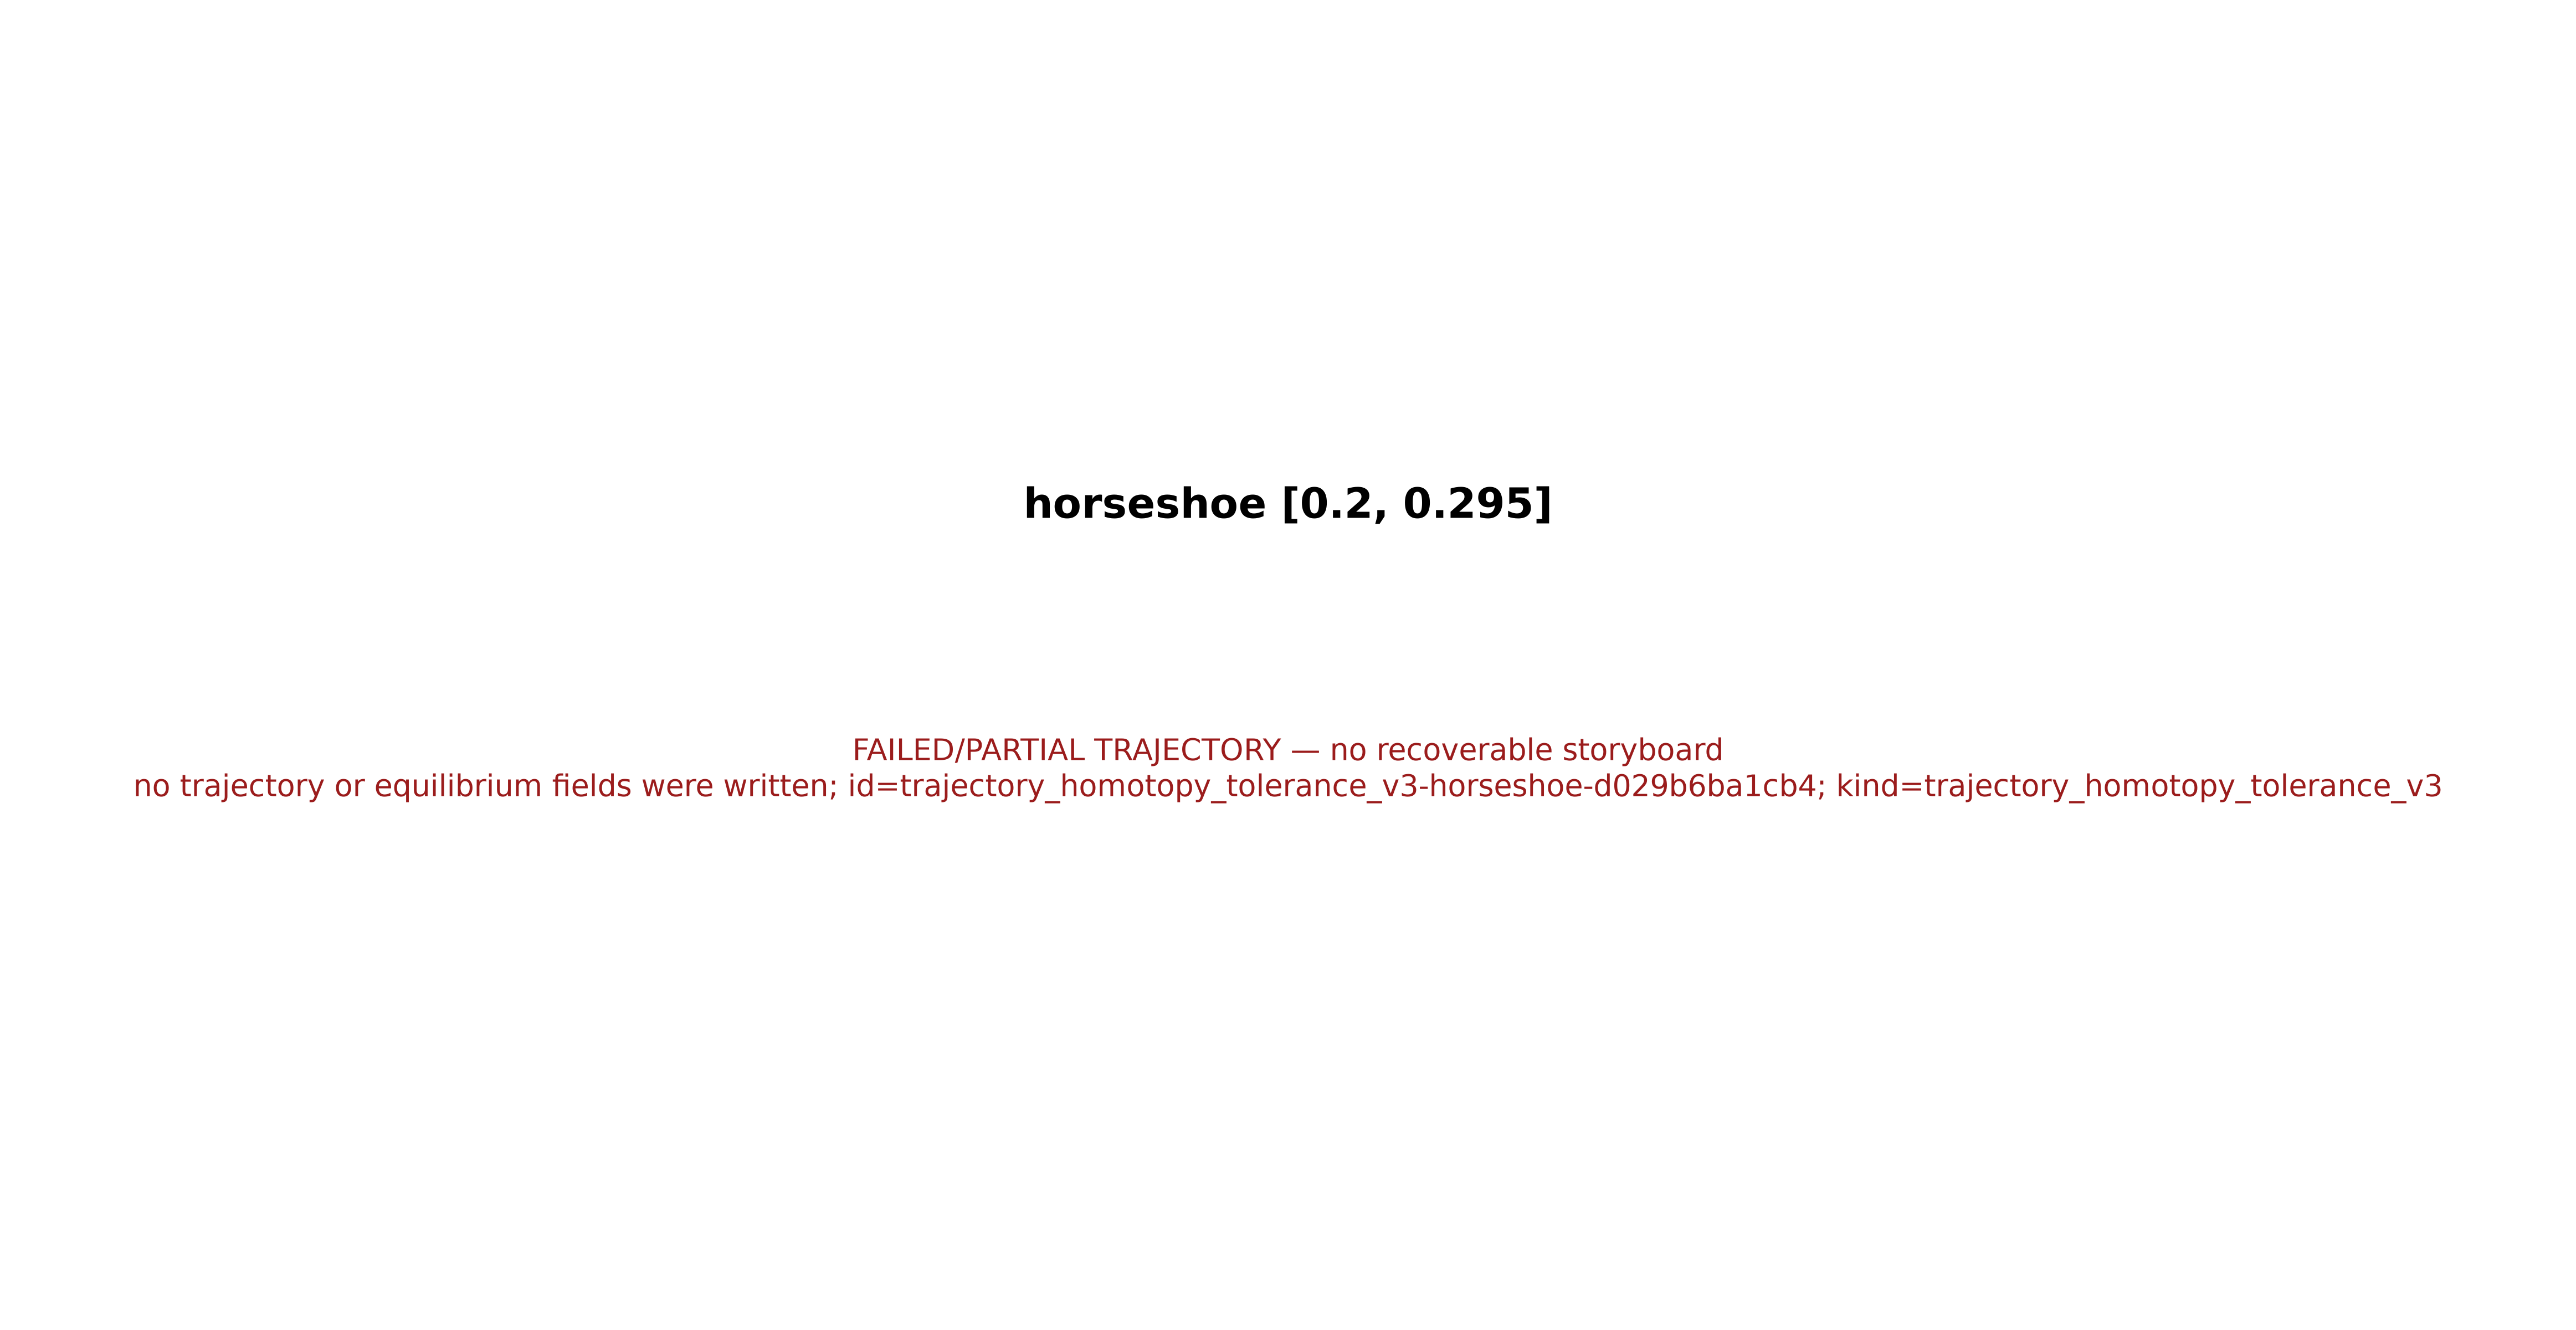
\includegraphics[width=0.88\linewidth]{figures/failed_band_evolution_030_horseshoe_0p2_0p295_trajectory_homotopy_tolerance_v3-horseshoe-d029b6ba1cb4.png}
\caption{Supplemental failed/partial trajectory evidence for horseshoe at torsion levels $[0.2,0.295]$ (case trajectory\_homotopy\_tolerance\_v3-horseshoe-d029b6ba1cb4; state=planned; classification=incomplete). The case is retained regardless of PDE or geometric success. Orange dashed curves are the fixed target band and blue solid curves are the moving equilibrium band; when state recovery is impossible, the PNG records the reason. Data status: diagnostic\_only.}
\label{fig:failed-storyboard-trajectory-homotopy-tolerance-v3-horseshoe-d029b6ba1cb4}
\end{figure}

\begin{figure}[tbp]
\centering
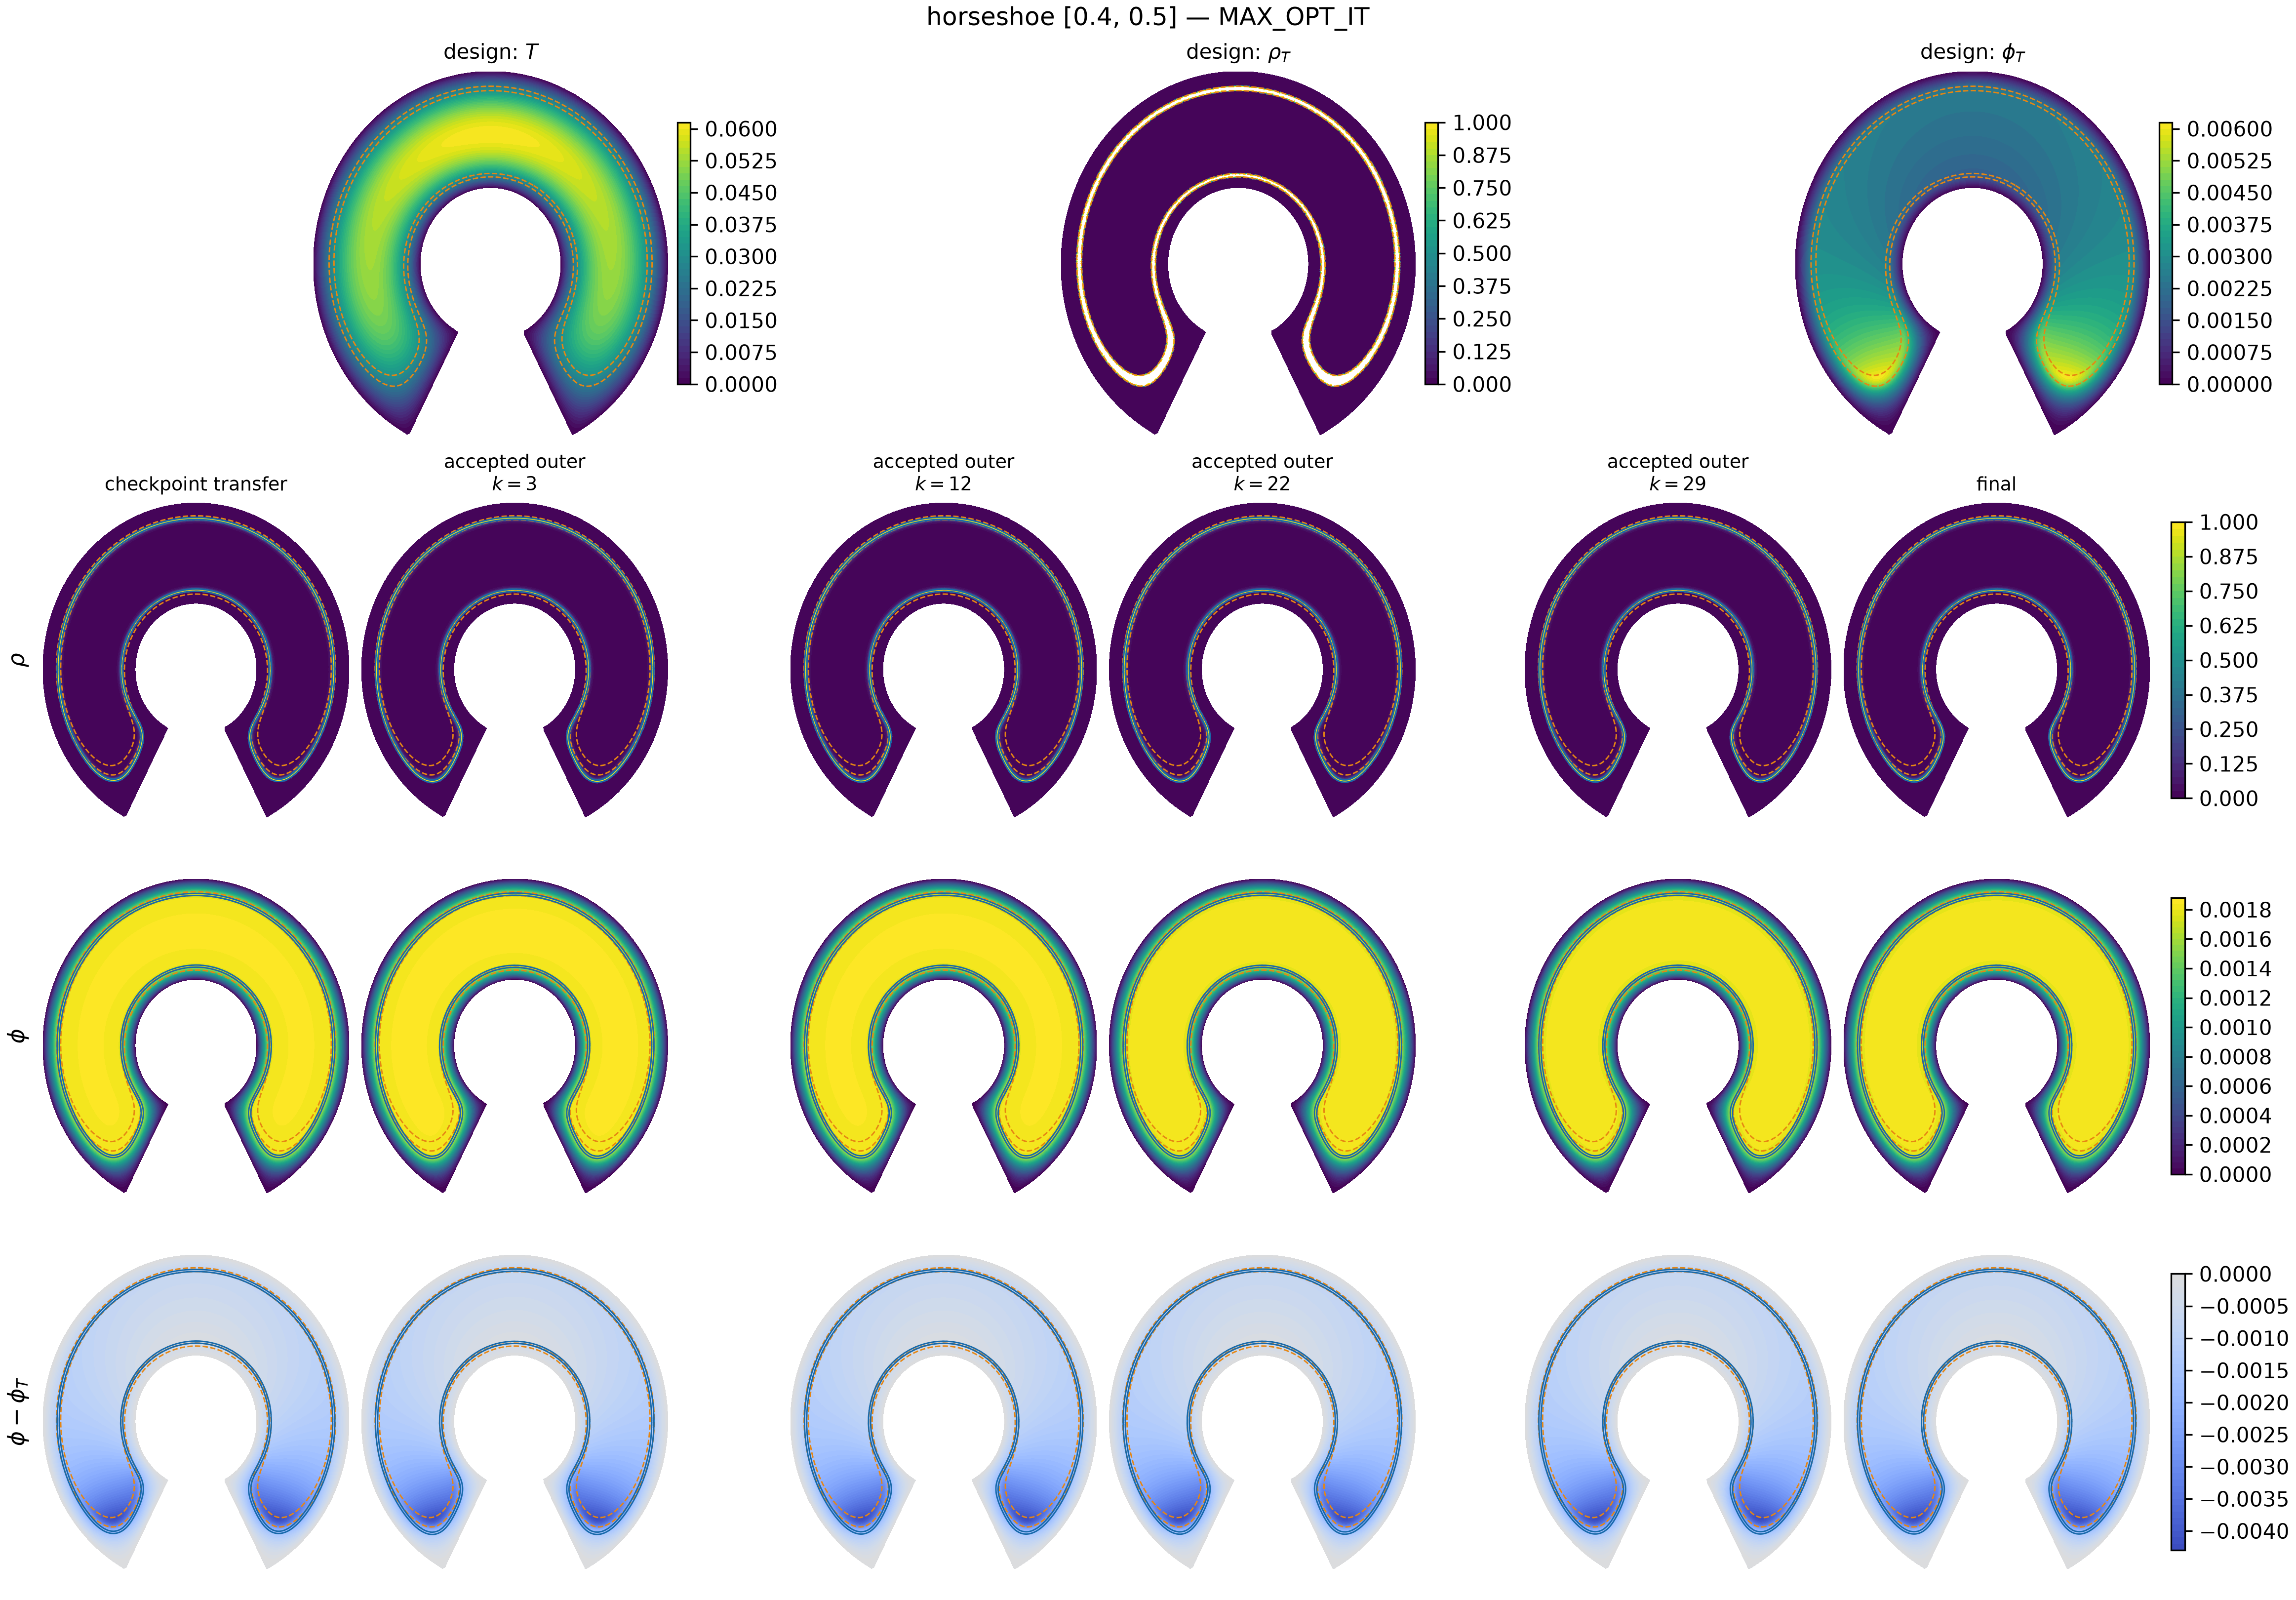
\includegraphics[width=0.88\linewidth]{figures/failed_band_evolution_031_horseshoe_0p4_0p5_trajectory_horseshoe_band_candidate_v3-horseshoe-dfba417fa450.png}
\caption{Supplemental failed/partial trajectory evidence for horseshoe at torsion levels $[0.4,0.5]$ (case trajectory\_horseshoe\_band\_candidate\_v3-horseshoe-dfba417fa450; state=completed; classification=geometrically\_unsuccessful\_pde\_converged). The case is retained regardless of PDE or geometric success. Orange dashed curves are the fixed target band and blue solid curves are the moving equilibrium band; when state recovery is impossible, the PNG records the reason. Data status: actual.}
\label{fig:failed-storyboard-trajectory-horseshoe-band-candidate-v3-horseshoe-dfba417fa450}
\end{figure}

\begin{figure}[tbp]
\centering
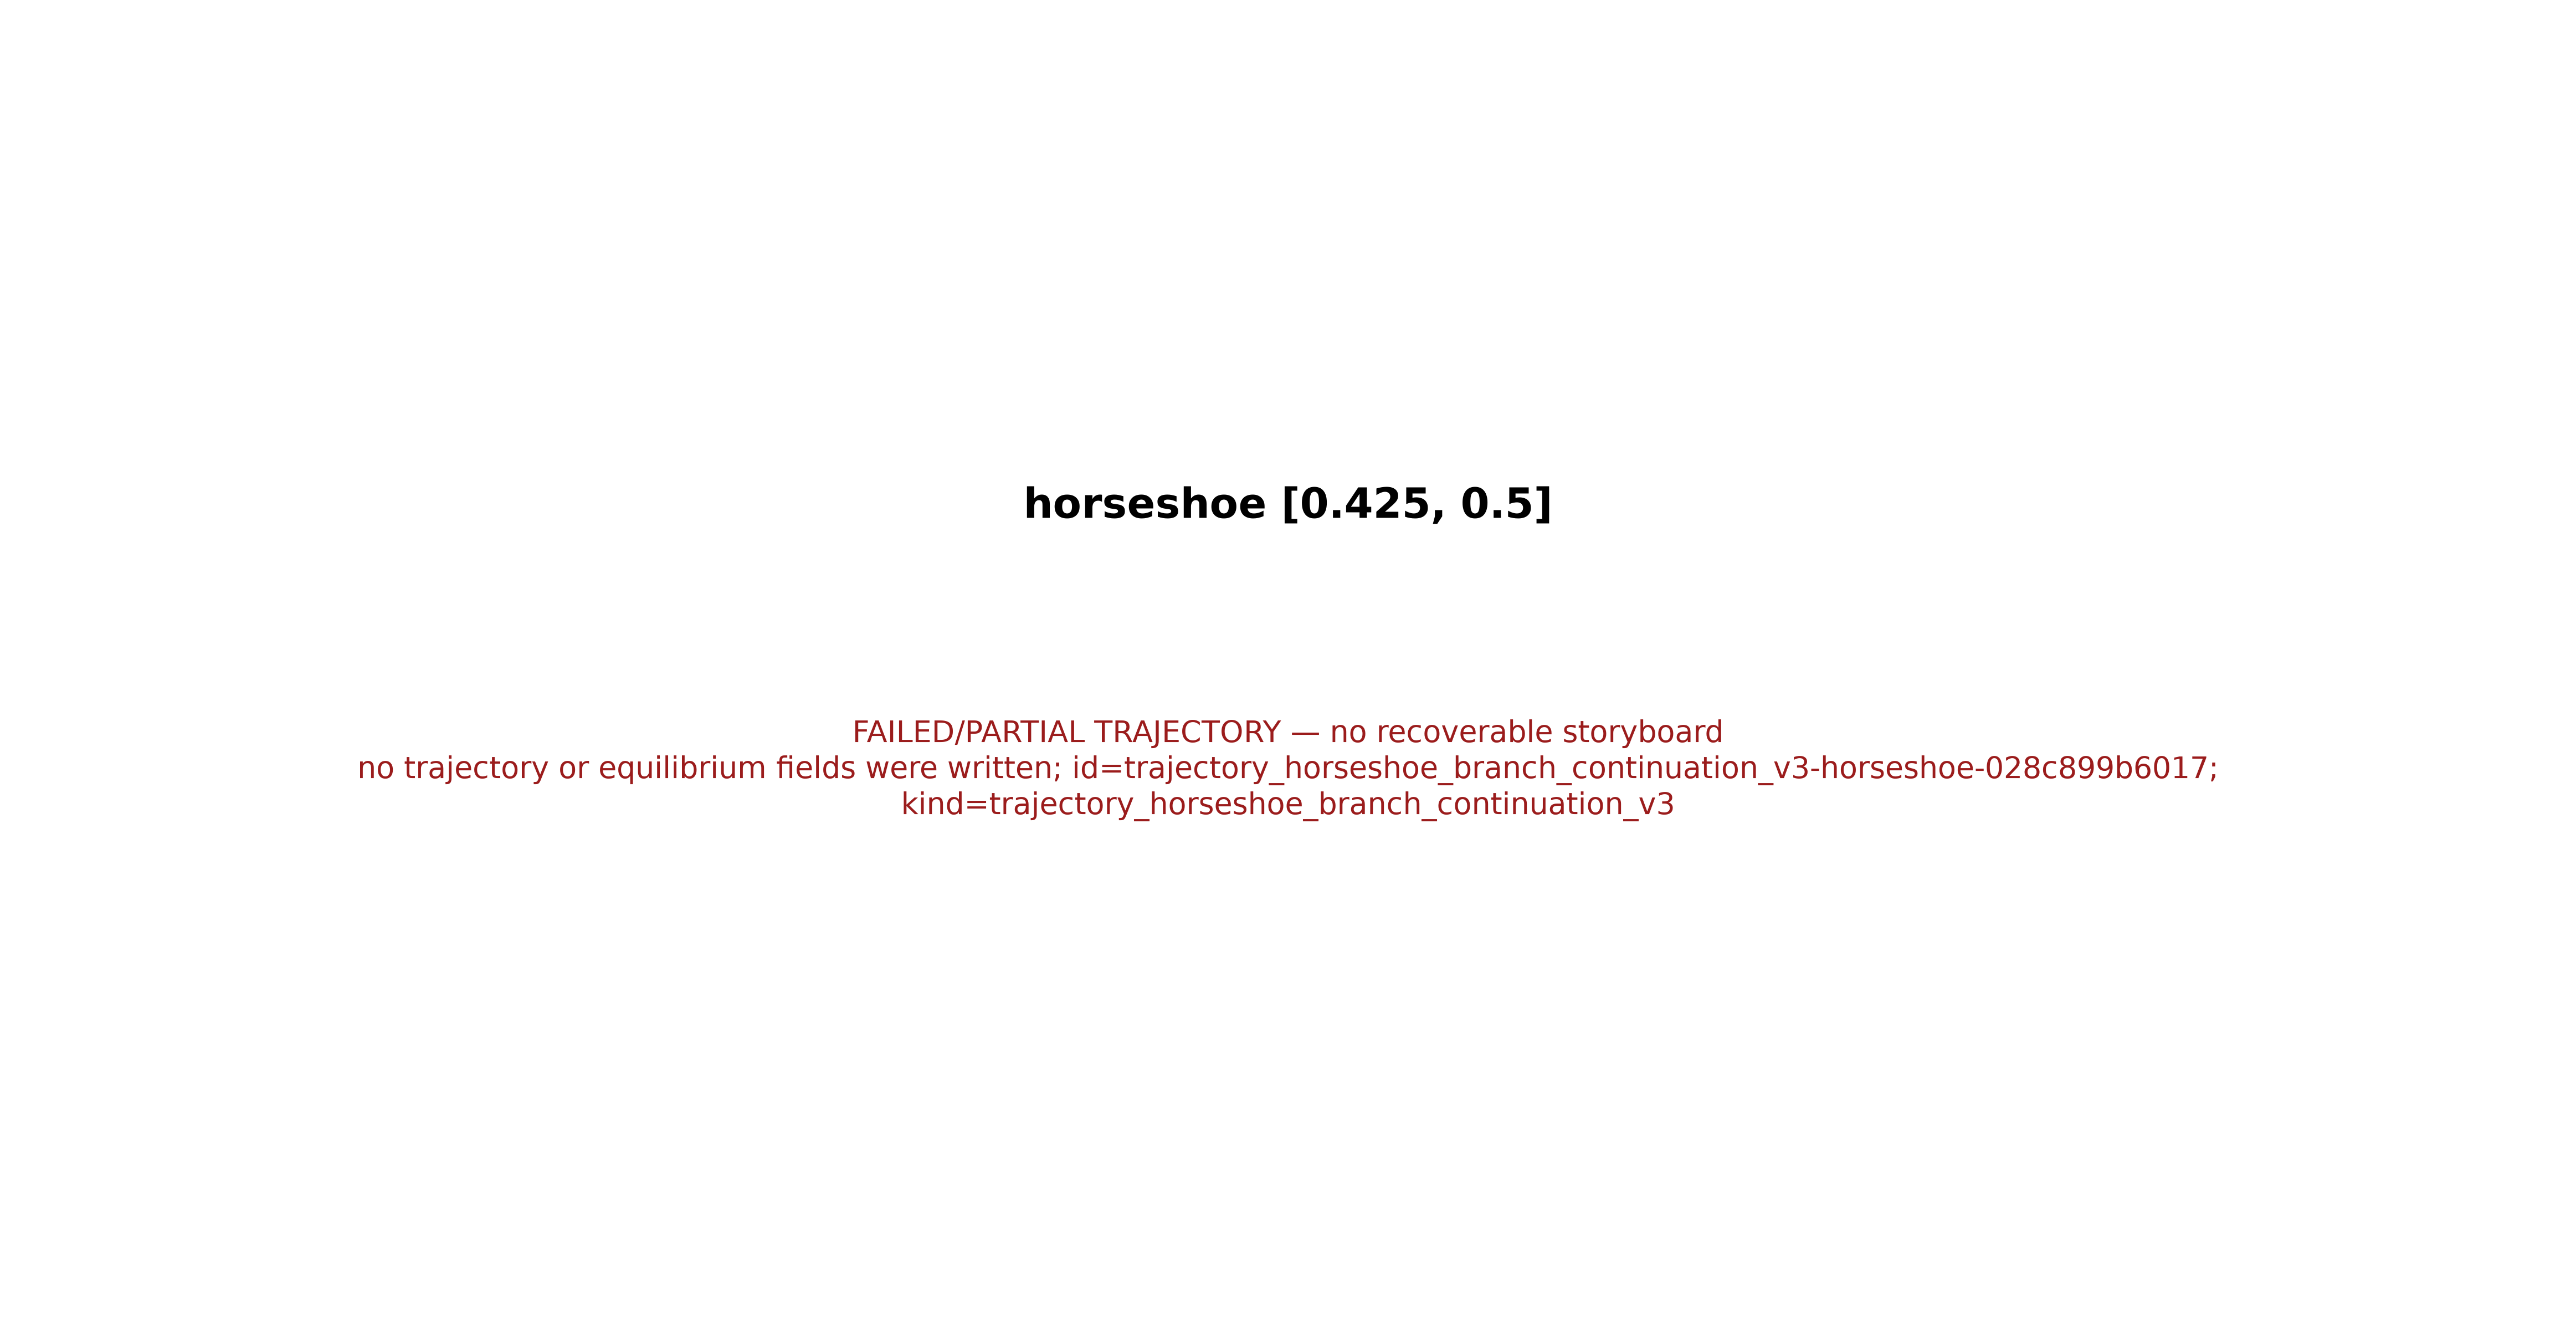
\includegraphics[width=0.88\linewidth]{figures/failed_band_evolution_032_horseshoe_0p425_0p5_trajectory_horseshoe_branch_continuation_v3-horseshoe-028c899b6017.png}
\caption{Supplemental failed/partial trajectory evidence for horseshoe at torsion levels $[0.425,0.5]$ (case trajectory\_horseshoe\_branch\_continuation\_v3-horseshoe-028c899b6017; state=planned; classification=incomplete). The case is retained regardless of PDE or geometric success. Orange dashed curves are the fixed target band and blue solid curves are the moving equilibrium band; when state recovery is impossible, the PNG records the reason. Data status: diagnostic\_only.}
\label{fig:failed-storyboard-trajectory-horseshoe-branch-continuation-v3-horseshoe-028c899b6017}
\end{figure}

\begin{figure}[tbp]
\centering
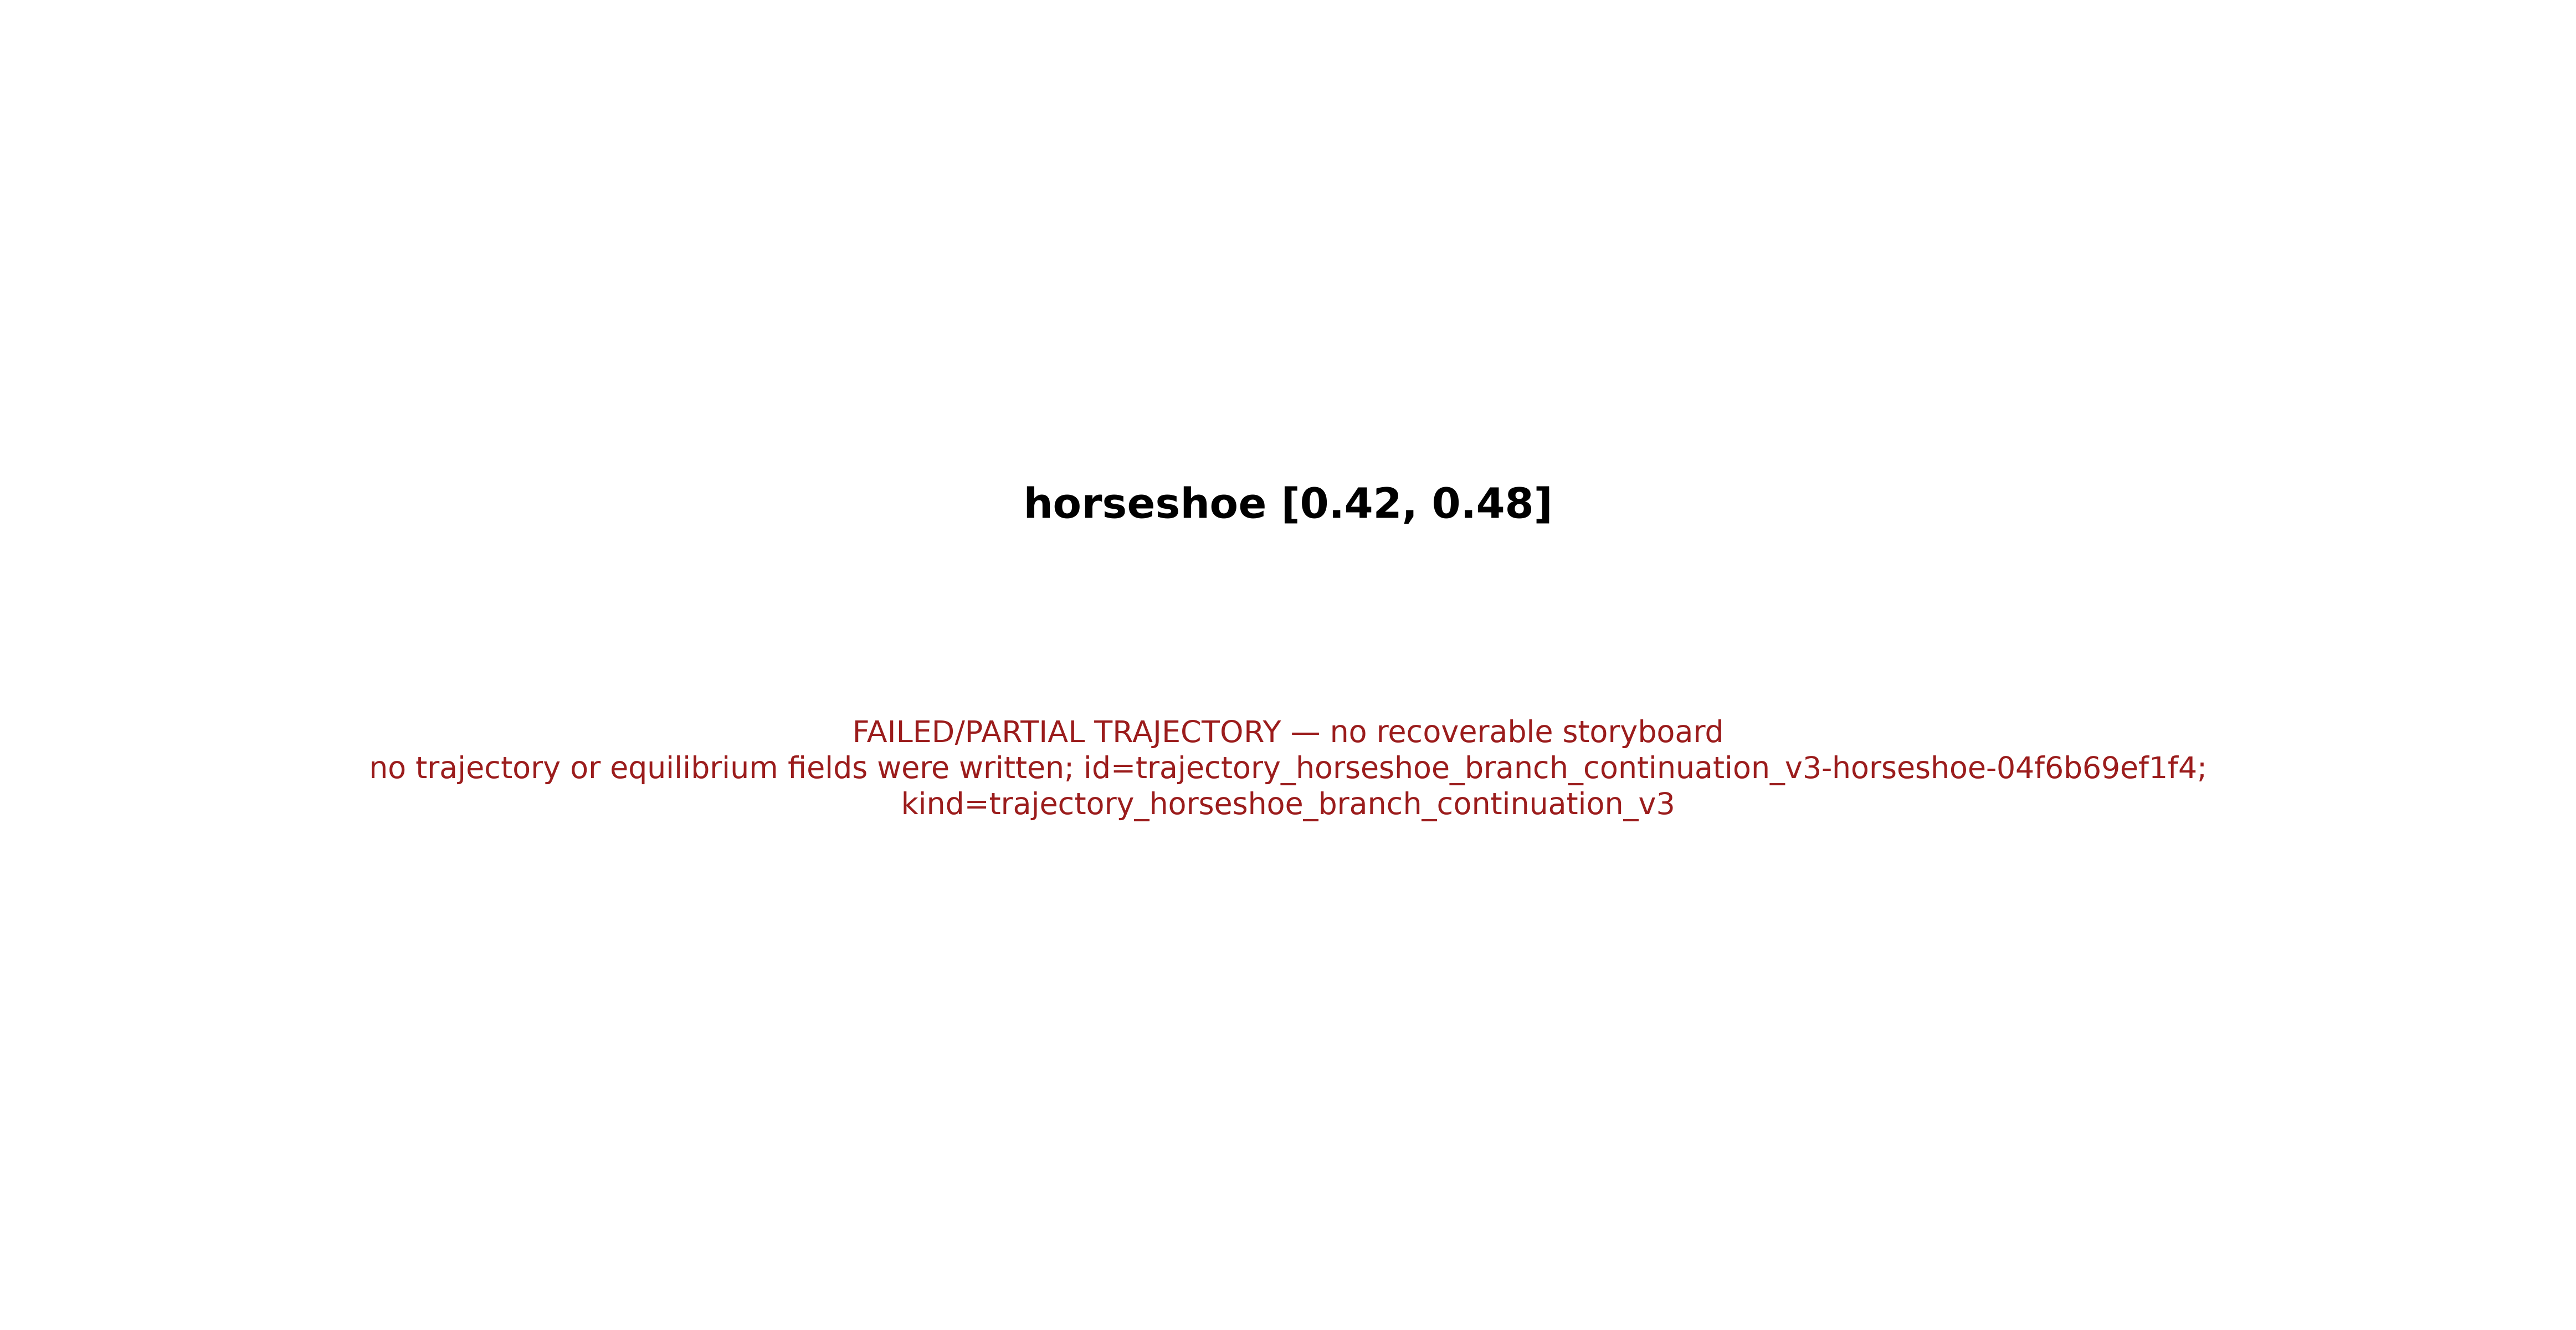
\includegraphics[width=0.88\linewidth]{figures/failed_band_evolution_033_horseshoe_0p42_0p48_trajectory_horseshoe_branch_continuation_v3-horseshoe-04f6b69ef1f4.png}
\caption{Supplemental failed/partial trajectory evidence for horseshoe at torsion levels $[0.42,0.48]$ (case trajectory\_horseshoe\_branch\_continuation\_v3-horseshoe-04f6b69ef1f4; state=planned; classification=incomplete). The case is retained regardless of PDE or geometric success. Orange dashed curves are the fixed target band and blue solid curves are the moving equilibrium band; when state recovery is impossible, the PNG records the reason. Data status: diagnostic\_only.}
\label{fig:failed-storyboard-trajectory-horseshoe-branch-continuation-v3-horseshoe-04f6b69ef1f4}
\end{figure}

\begin{figure}[tbp]
\centering
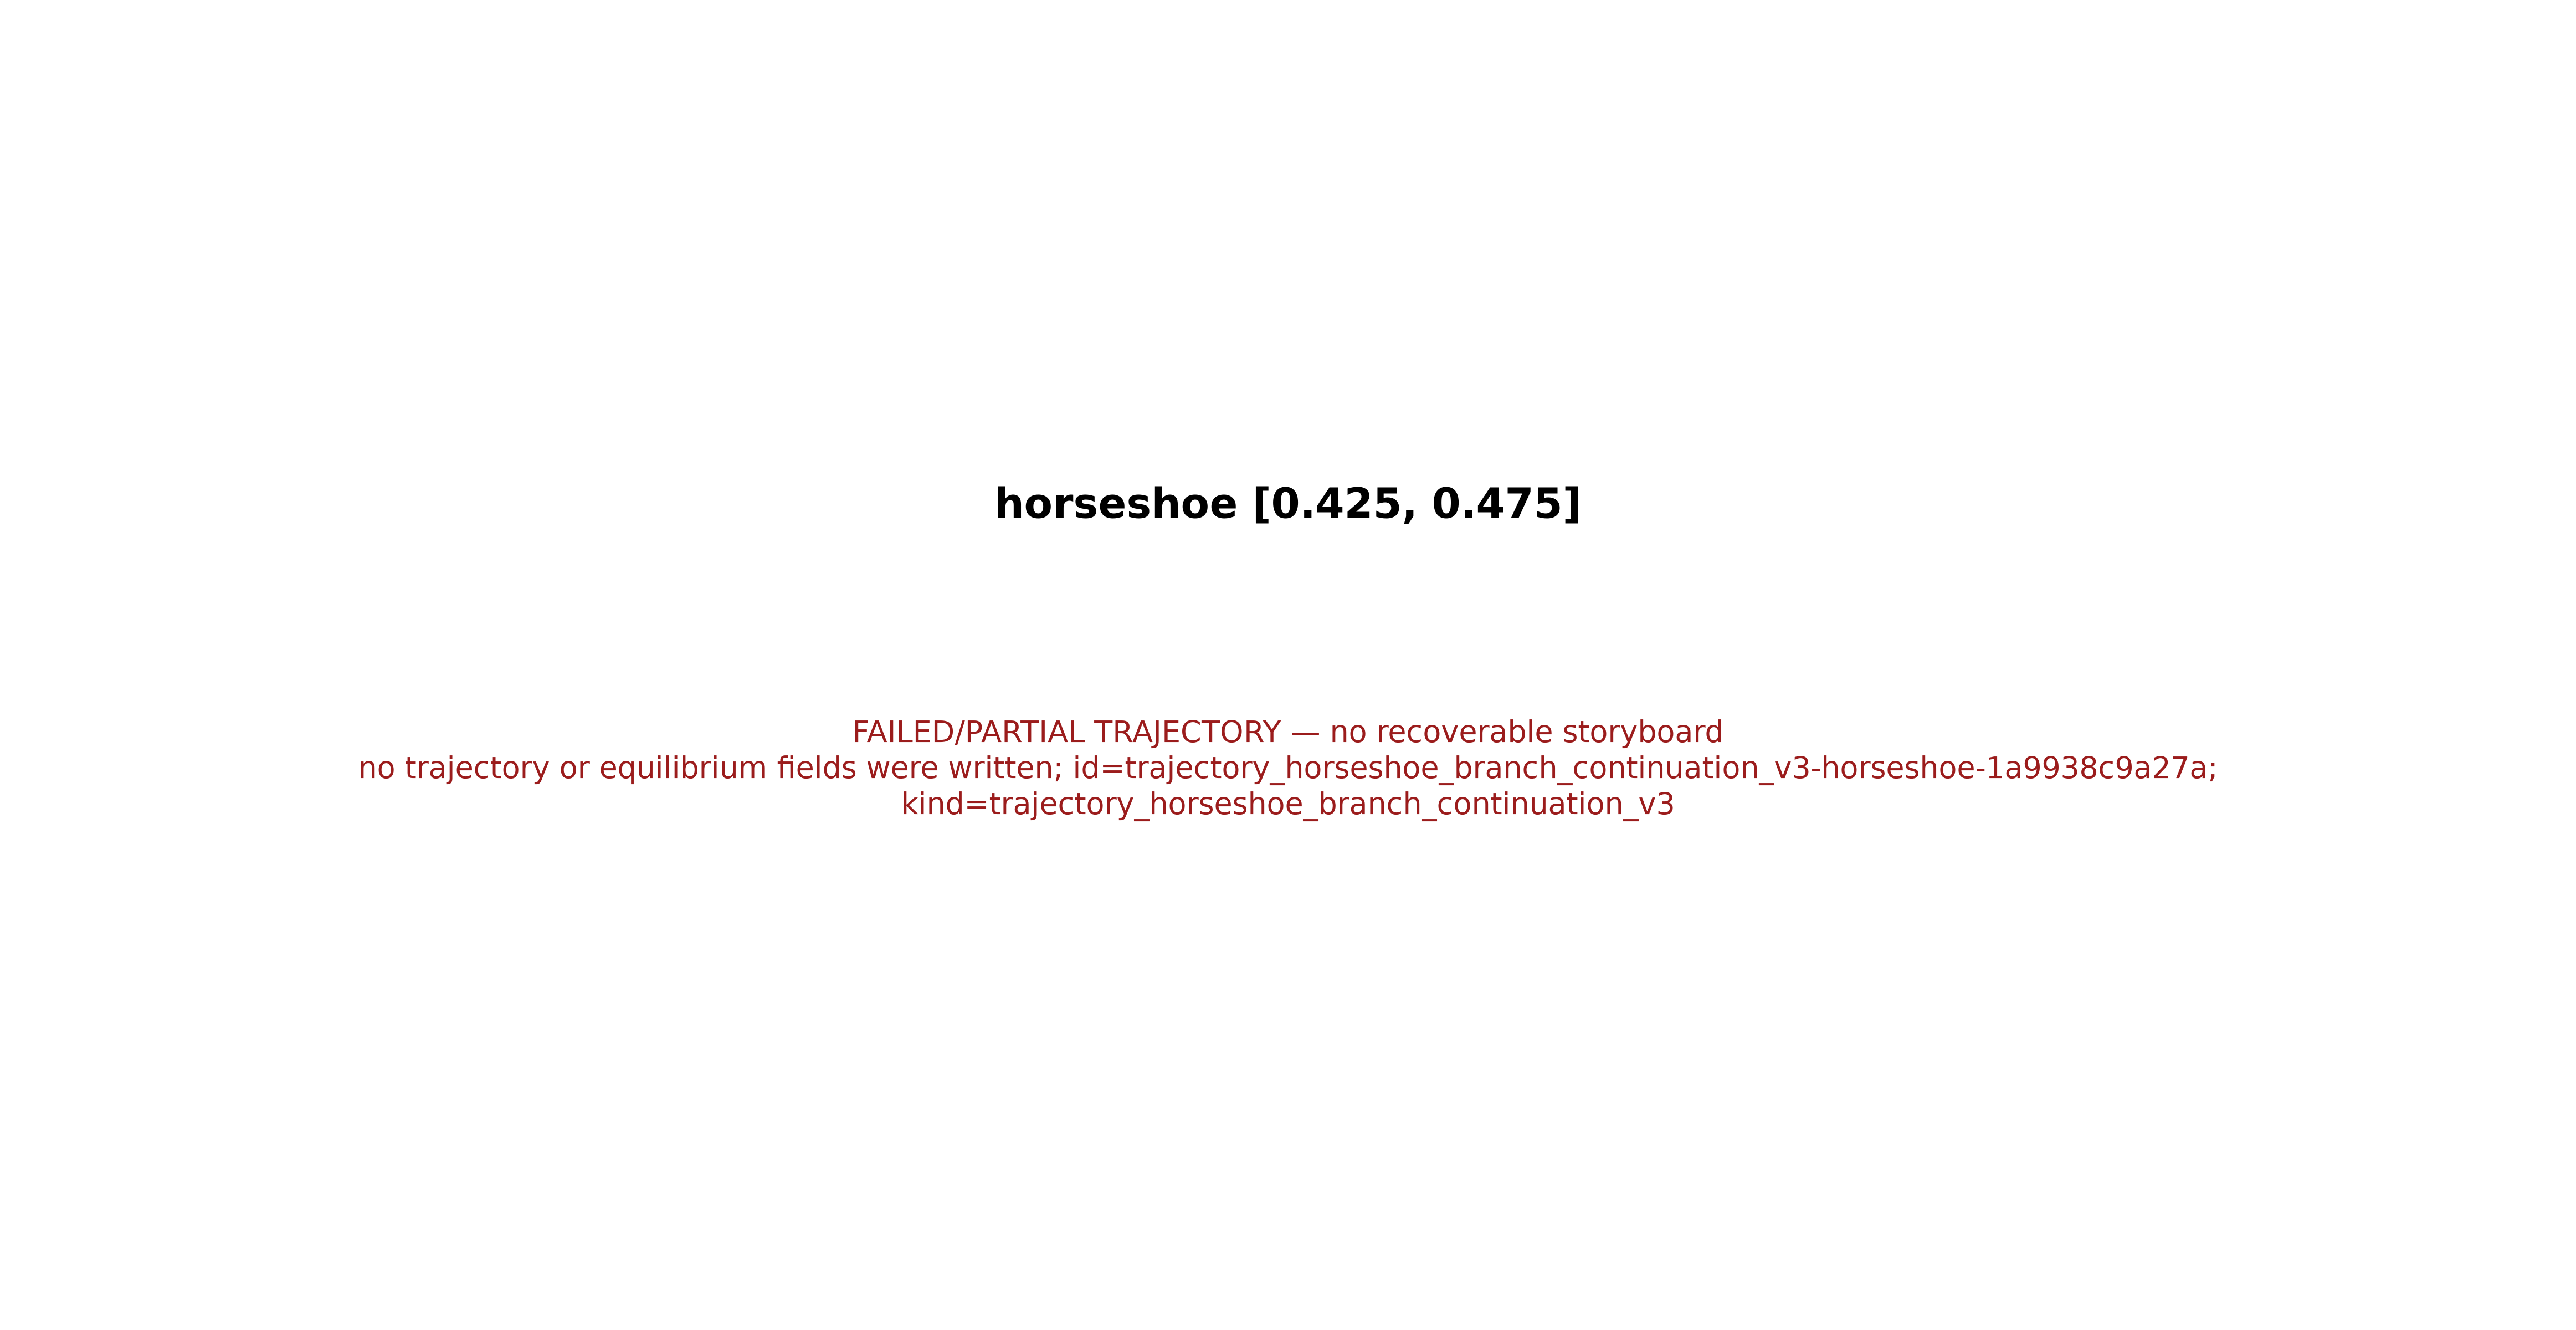
\includegraphics[width=0.88\linewidth]{figures/failed_band_evolution_034_horseshoe_0p425_0p475_trajectory_horseshoe_branch_continuation_v3-horseshoe-1a9938c9a27a.png}
\caption{Supplemental failed/partial trajectory evidence for horseshoe at torsion levels $[0.425,0.475]$ (case trajectory\_horseshoe\_branch\_continuation\_v3-horseshoe-1a9938c9a27a; state=planned; classification=incomplete). The case is retained regardless of PDE or geometric success. Orange dashed curves are the fixed target band and blue solid curves are the moving equilibrium band; when state recovery is impossible, the PNG records the reason. Data status: diagnostic\_only.}
\label{fig:failed-storyboard-trajectory-horseshoe-branch-continuation-v3-horseshoe-1a9938c9a27a}
\end{figure}

\begin{figure}[tbp]
\centering
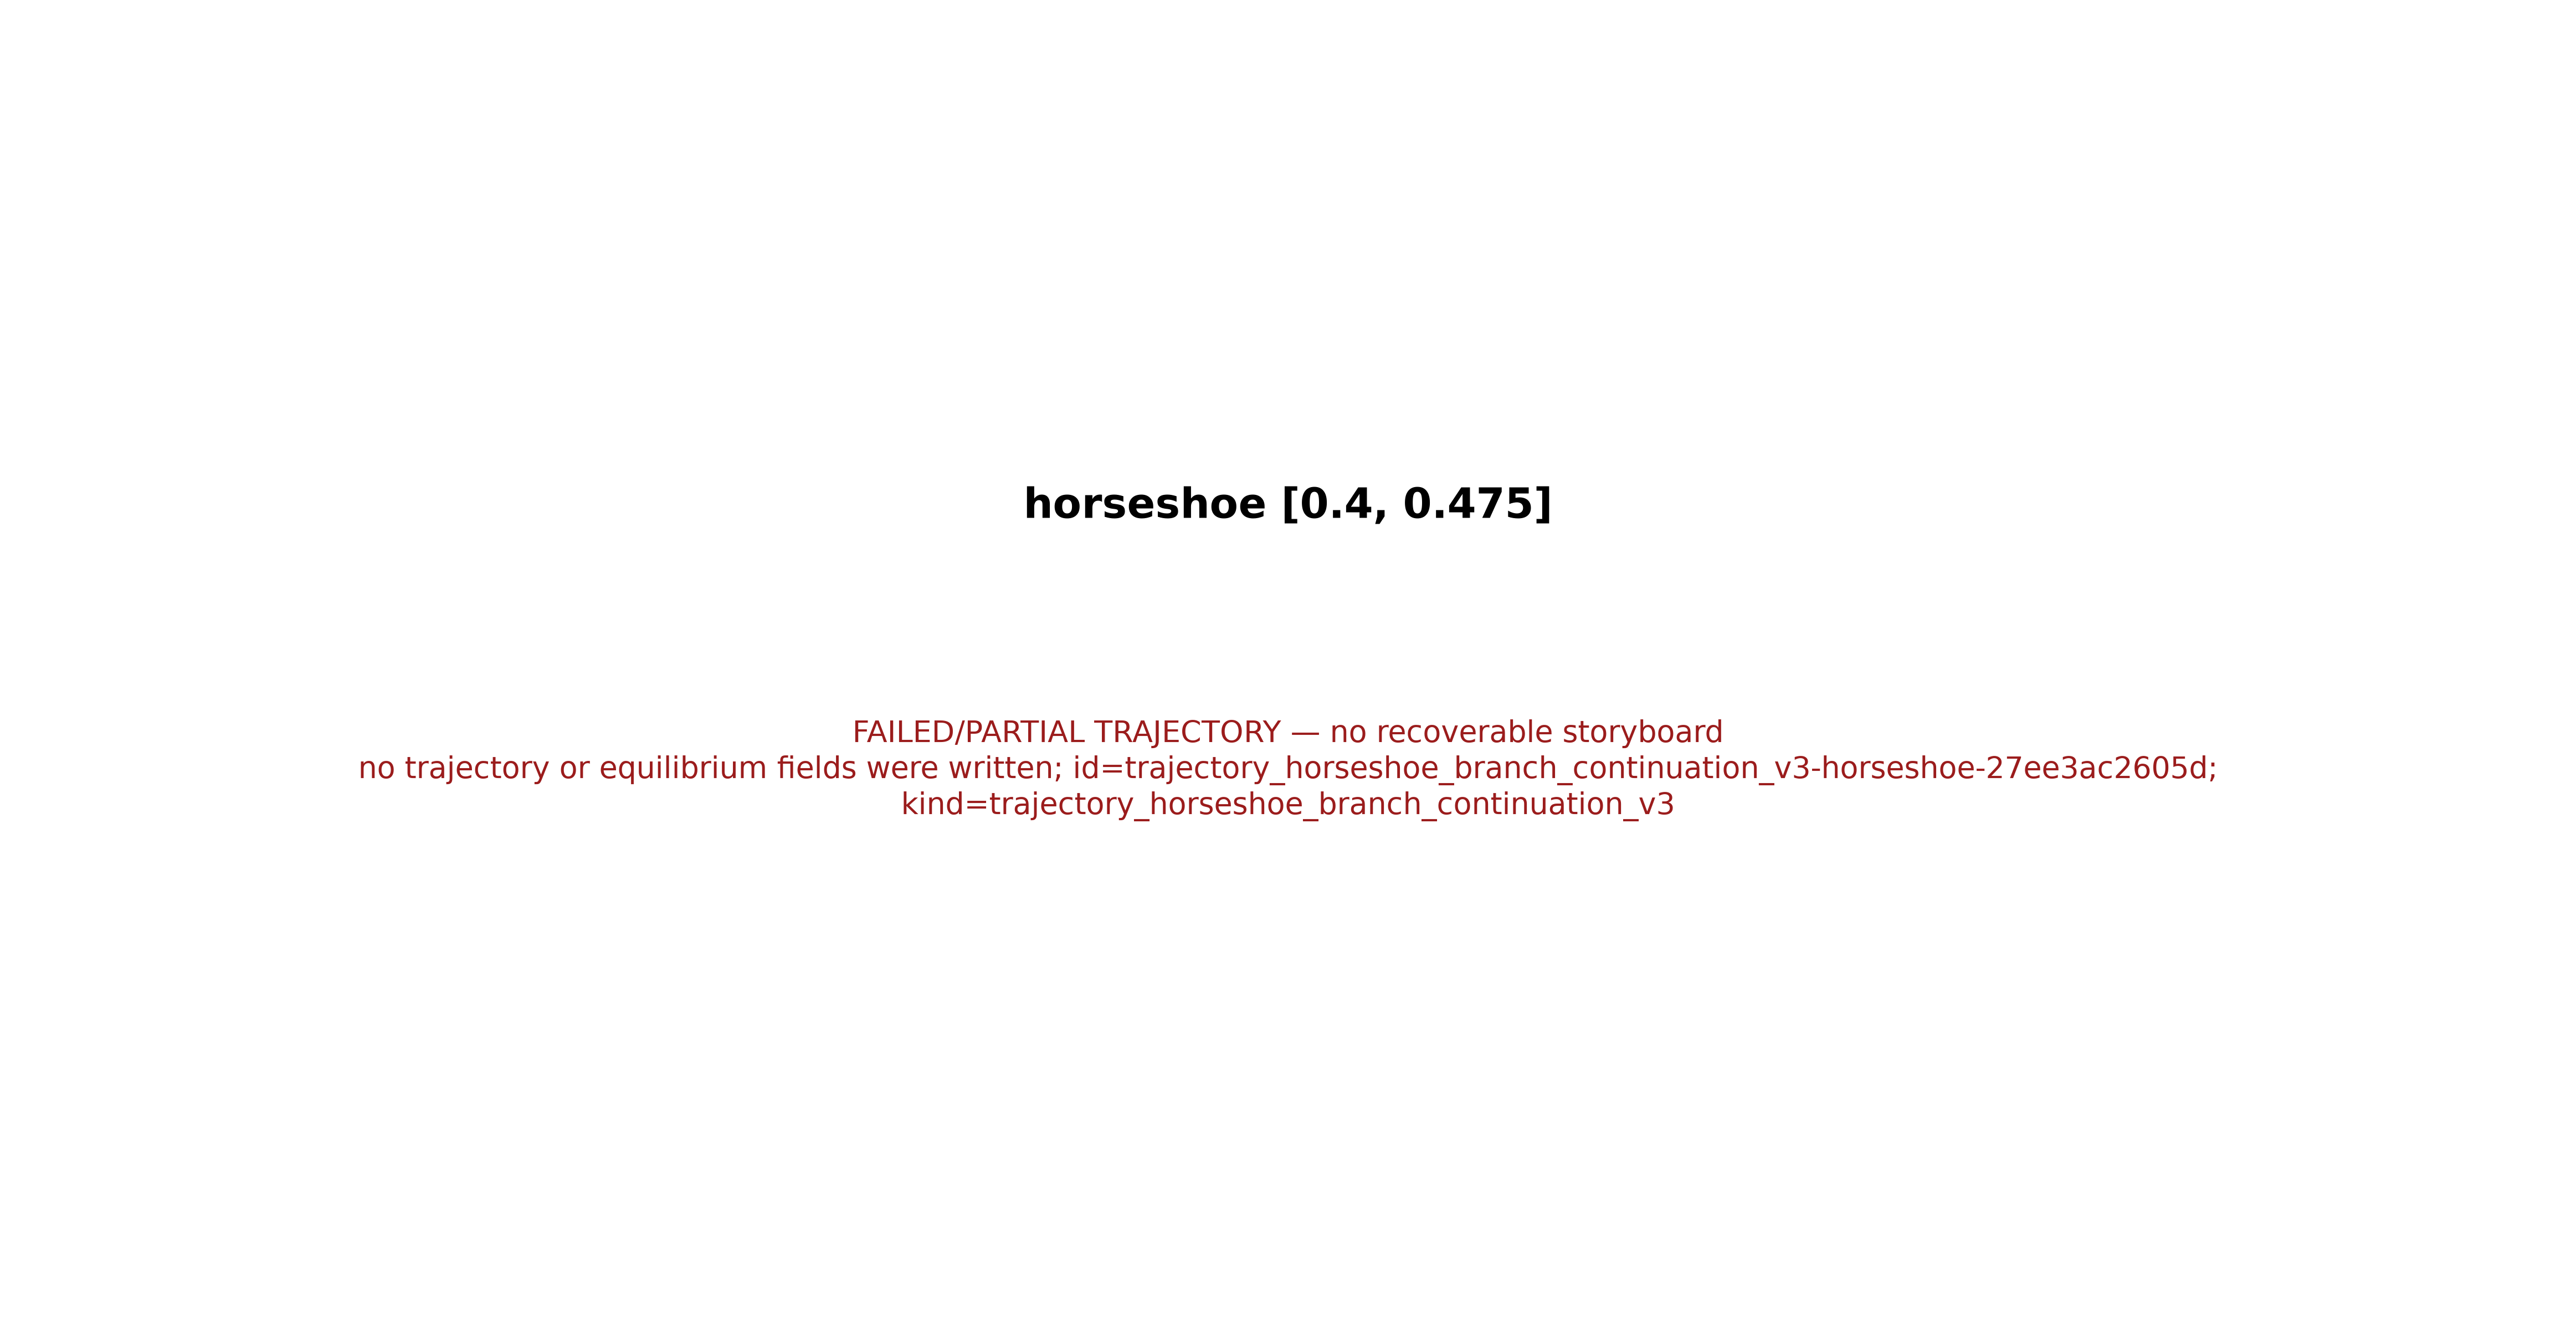
\includegraphics[width=0.88\linewidth]{figures/failed_band_evolution_035_horseshoe_0p4_0p475_trajectory_horseshoe_branch_continuation_v3-horseshoe-27ee3ac2605d.png}
\caption{Supplemental failed/partial trajectory evidence for horseshoe at torsion levels $[0.4,0.475]$ (case trajectory\_horseshoe\_branch\_continuation\_v3-horseshoe-27ee3ac2605d; state=planned; classification=incomplete). The case is retained regardless of PDE or geometric success. Orange dashed curves are the fixed target band and blue solid curves are the moving equilibrium band; when state recovery is impossible, the PNG records the reason. Data status: diagnostic\_only.}
\label{fig:failed-storyboard-trajectory-horseshoe-branch-continuation-v3-horseshoe-27ee3ac2605d}
\end{figure}

\begin{figure}[tbp]
\centering
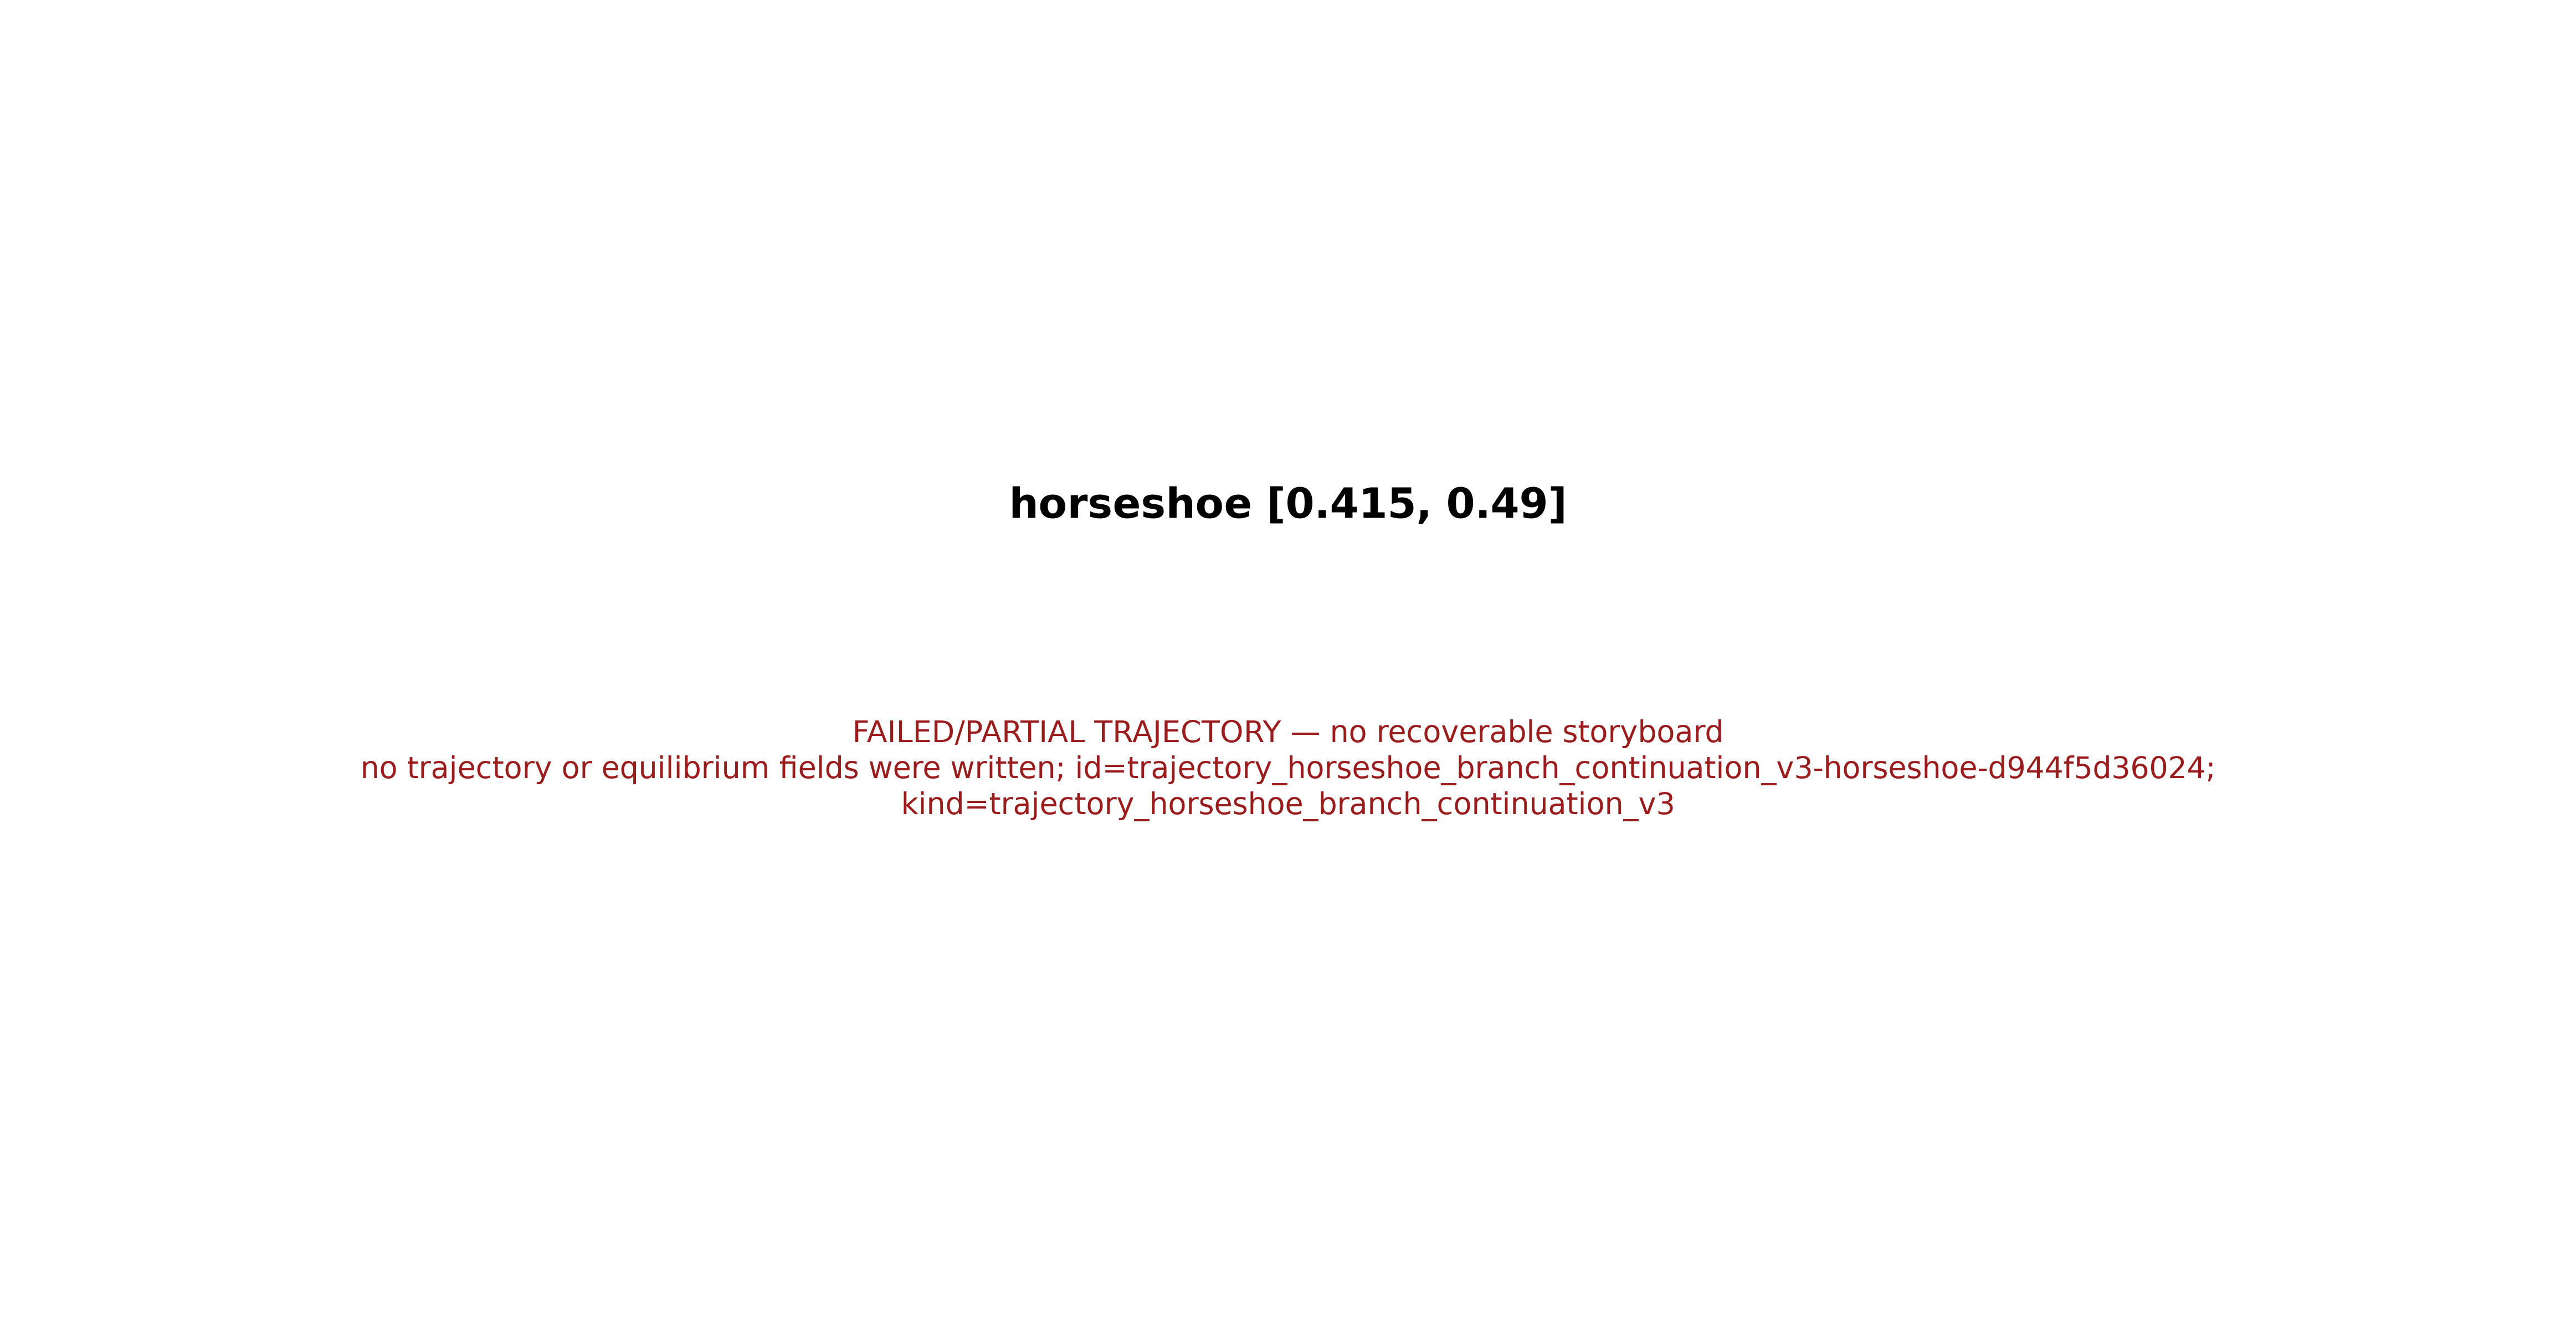
\includegraphics[width=0.88\linewidth]{figures/failed_band_evolution_036_horseshoe_0p415_0p49_trajectory_horseshoe_branch_continuation_v3-horseshoe-d944f5d36024.png}
\caption{Supplemental failed/partial trajectory evidence for horseshoe at torsion levels $[0.415,0.49]$ (case trajectory\_horseshoe\_branch\_continuation\_v3-horseshoe-d944f5d36024; state=planned; classification=incomplete). The case is retained regardless of PDE or geometric success. Orange dashed curves are the fixed target band and blue solid curves are the moving equilibrium band; when state recovery is impossible, the PNG records the reason. Data status: diagnostic\_only.}
\label{fig:failed-storyboard-trajectory-horseshoe-branch-continuation-v3-horseshoe-d944f5d36024}
\end{figure}

\begin{figure}[tbp]
\centering
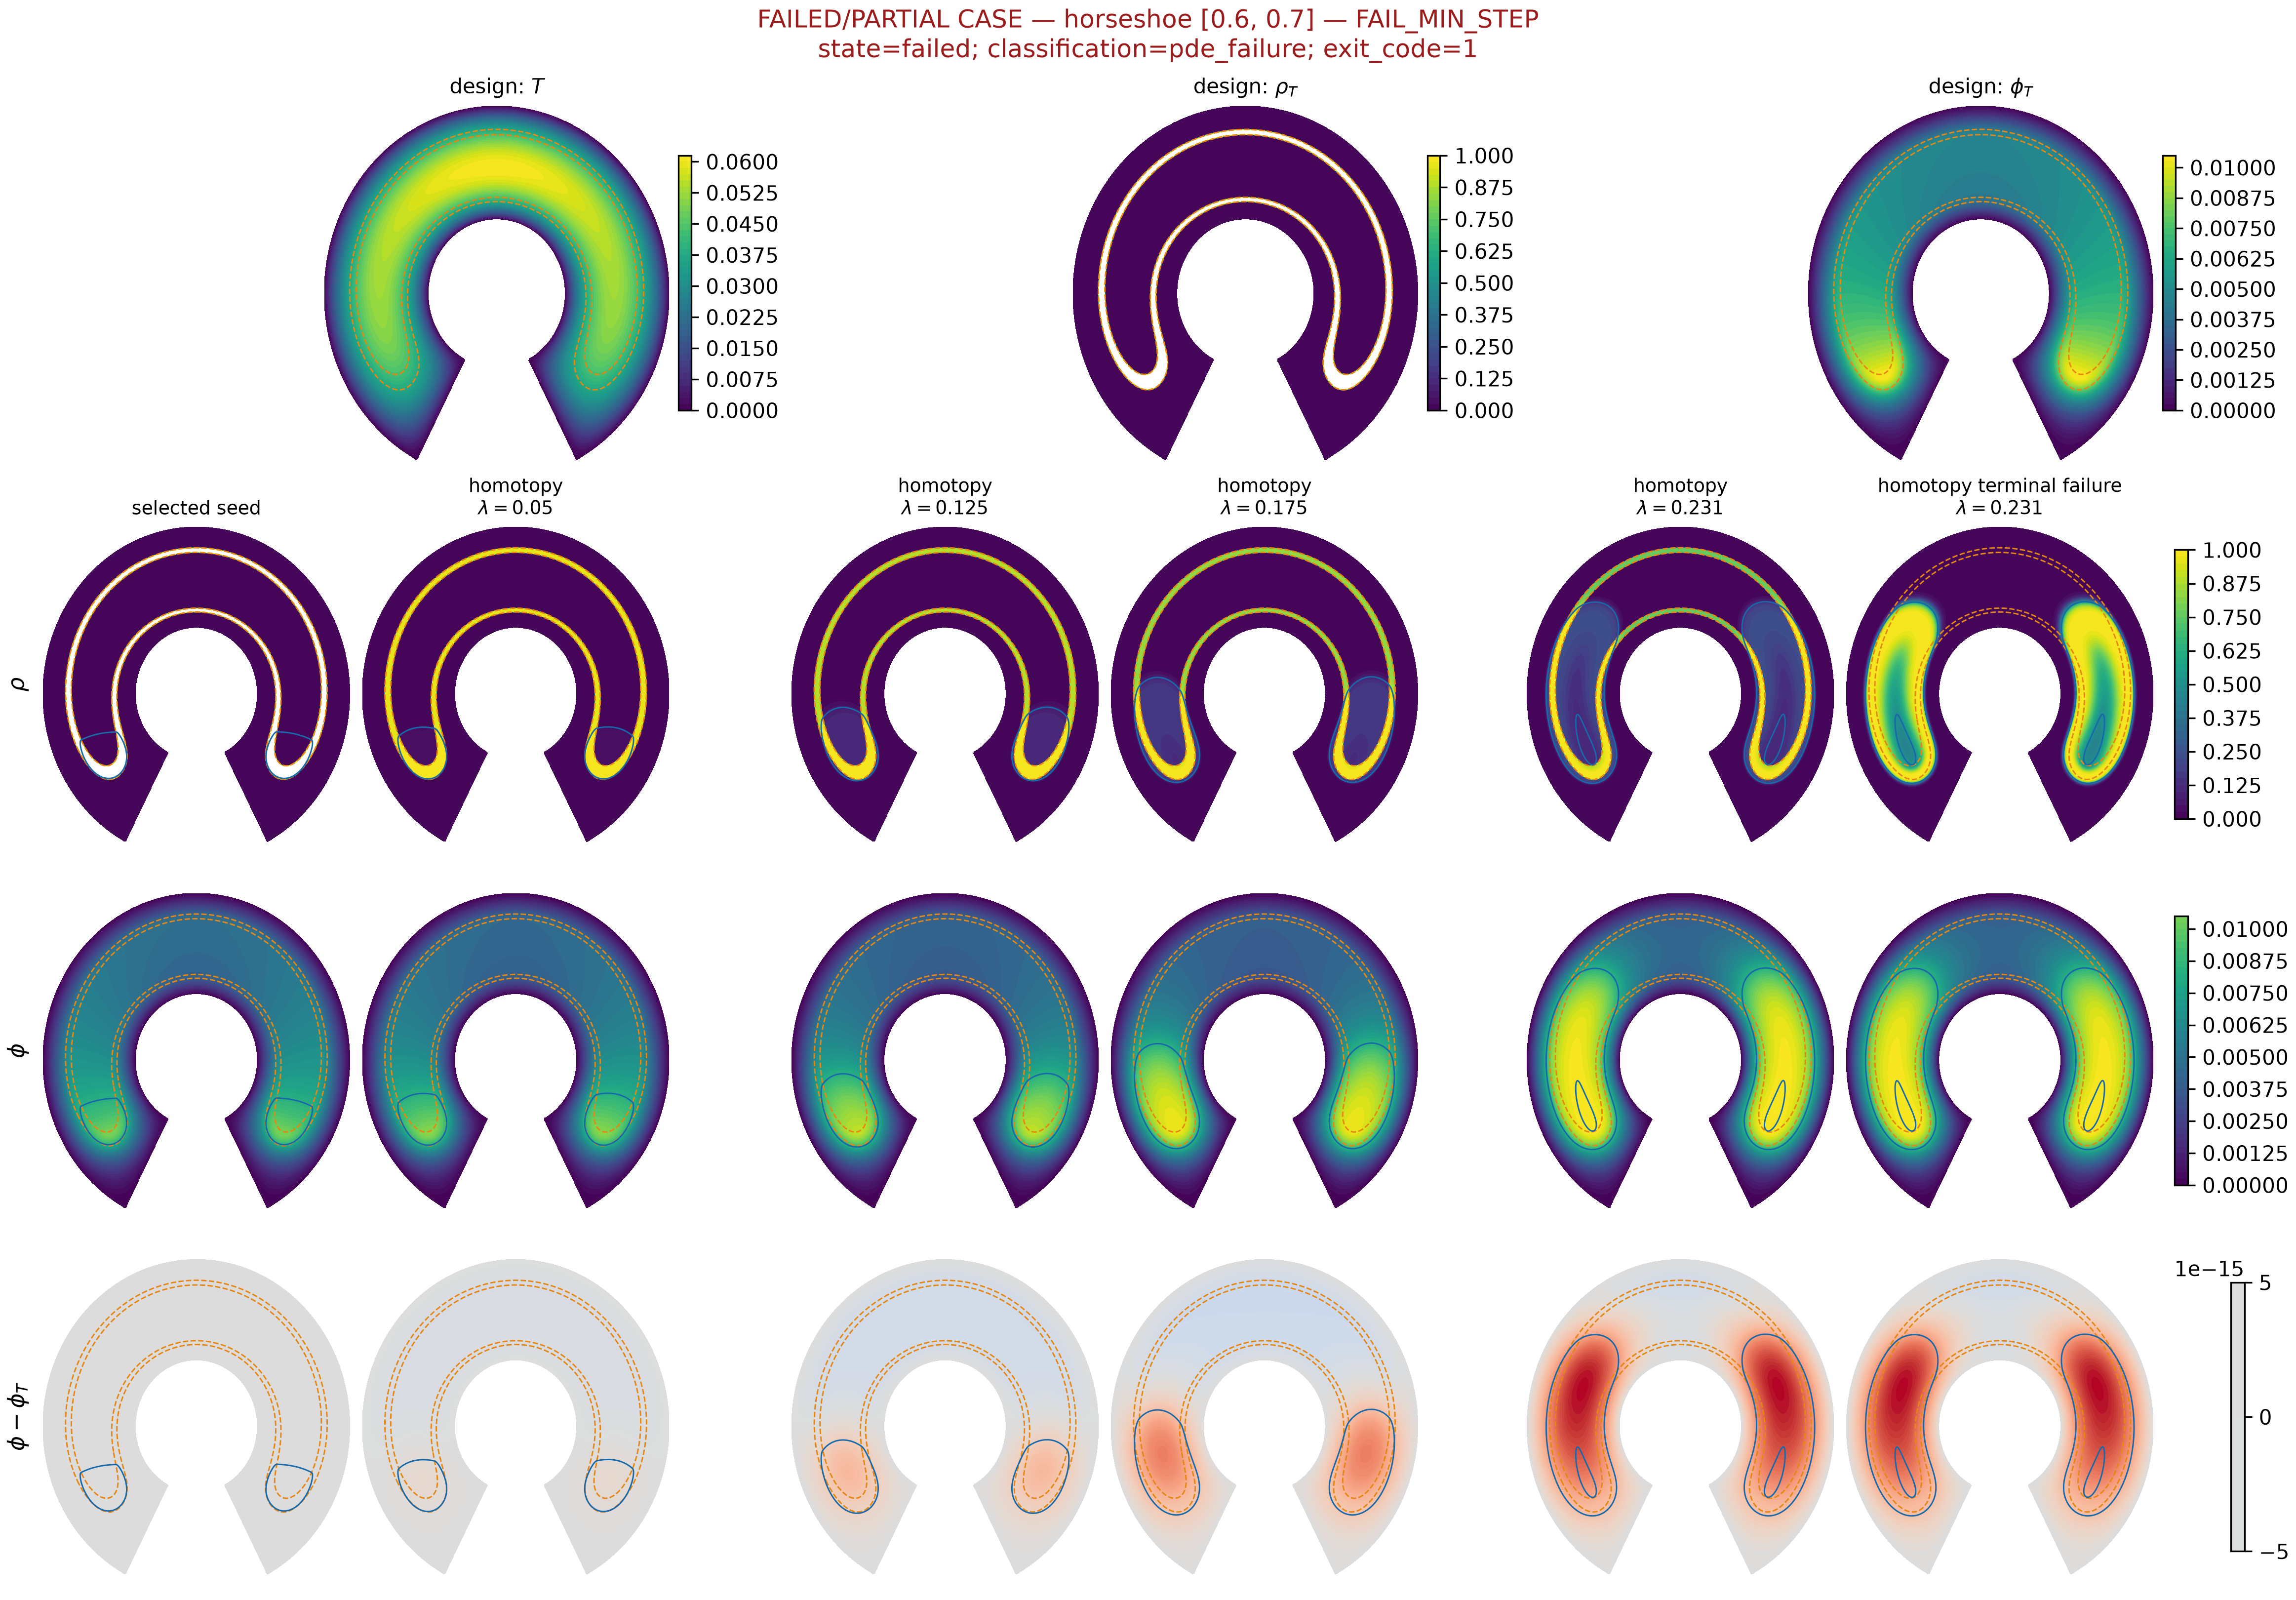
\includegraphics[width=0.88\linewidth]{figures/failed_band_evolution_037_horseshoe_0p6_0p7_trajectory_rescue-horseshoe-36a04ba8a51c.png}
\caption{Supplemental failed/partial trajectory evidence for horseshoe at torsion levels $[0.6,0.7]$ (case trajectory\_rescue-horseshoe-36a04ba8a51c; state=failed; classification=pde\_failure). The case is retained regardless of PDE or geometric success. Orange dashed curves are the fixed target band and blue solid curves are the moving equilibrium band; when state recovery is impossible, the PNG records the reason. Data status: actual.}
\label{fig:failed-storyboard-trajectory-rescue-horseshoe-36a04ba8a51c}
\end{figure}

\clearpage

\begin{figure}[tbp]
\centering
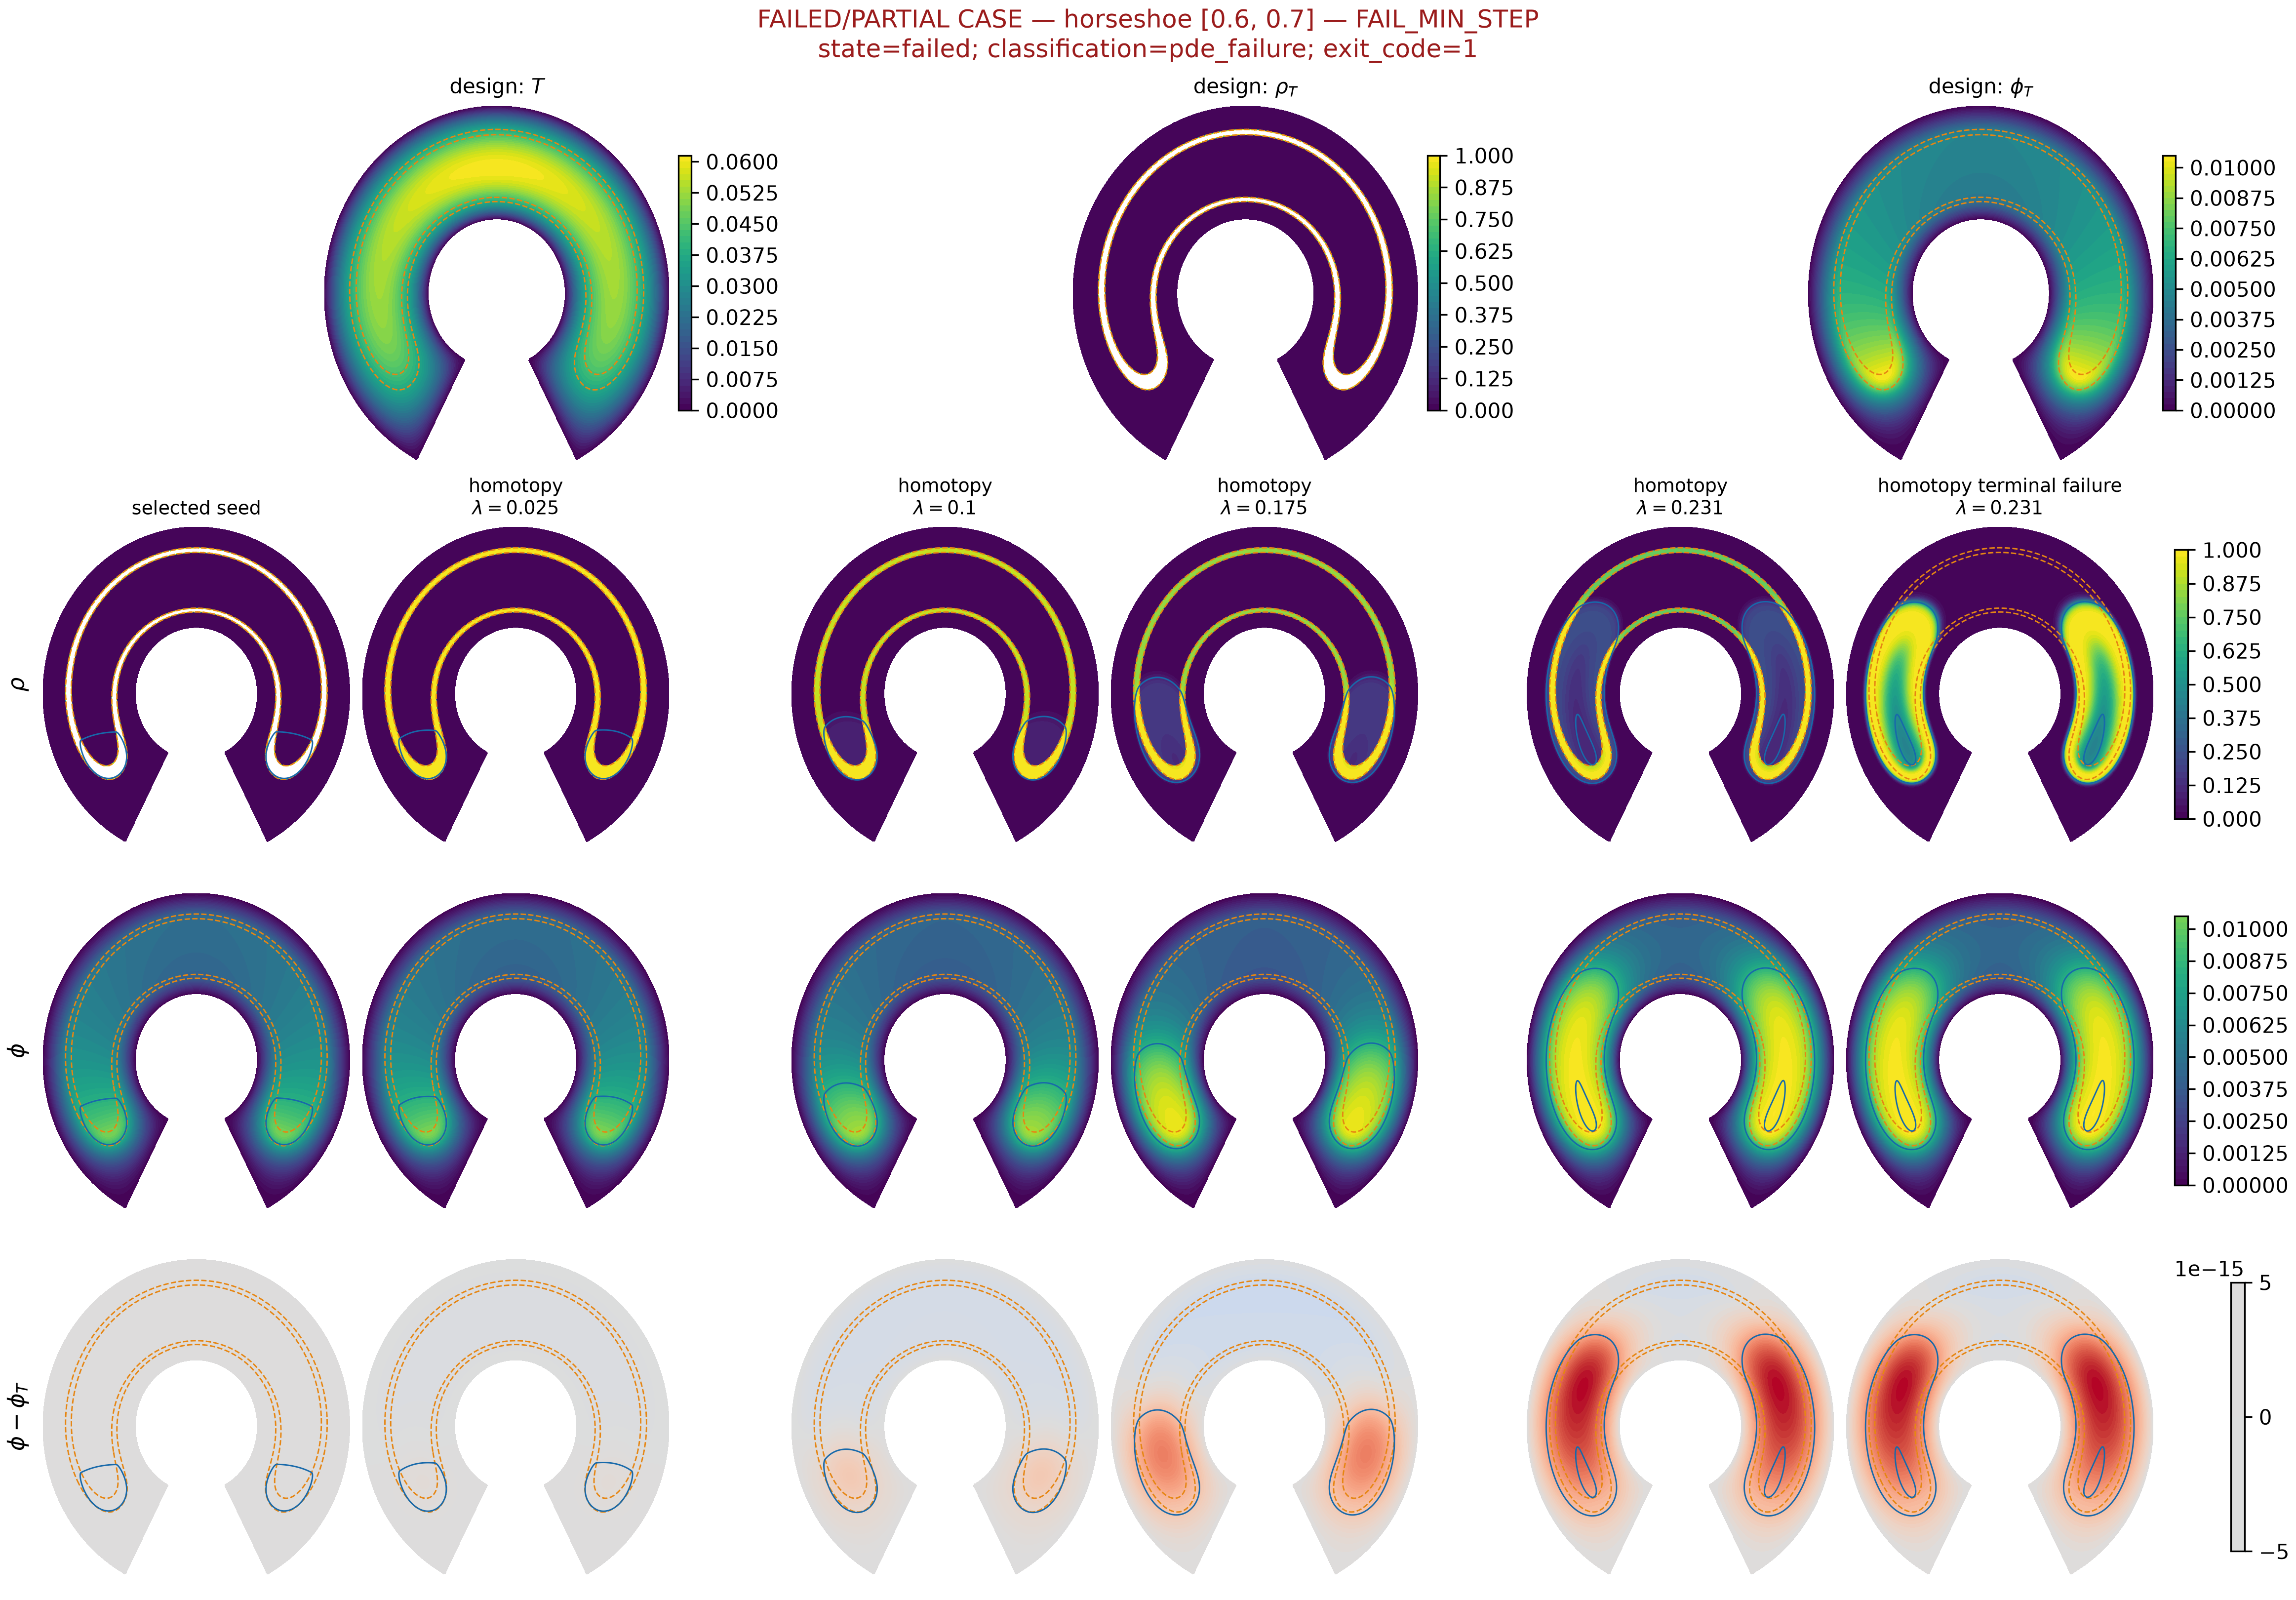
\includegraphics[width=0.88\linewidth]{figures/failed_band_evolution_038_horseshoe_0p6_0p7_trajectory_rescue-horseshoe-aeafd218049f.png}
\caption{Supplemental failed/partial trajectory evidence for horseshoe at torsion levels $[0.6,0.7]$ (case trajectory\_rescue-horseshoe-aeafd218049f; state=failed; classification=pde\_failure). The case is retained regardless of PDE or geometric success. Orange dashed curves are the fixed target band and blue solid curves are the moving equilibrium band; when state recovery is impossible, the PNG records the reason. Data status: actual.}
\label{fig:failed-storyboard-trajectory-rescue-horseshoe-aeafd218049f}
\end{figure}

\begin{figure}[tbp]
\centering
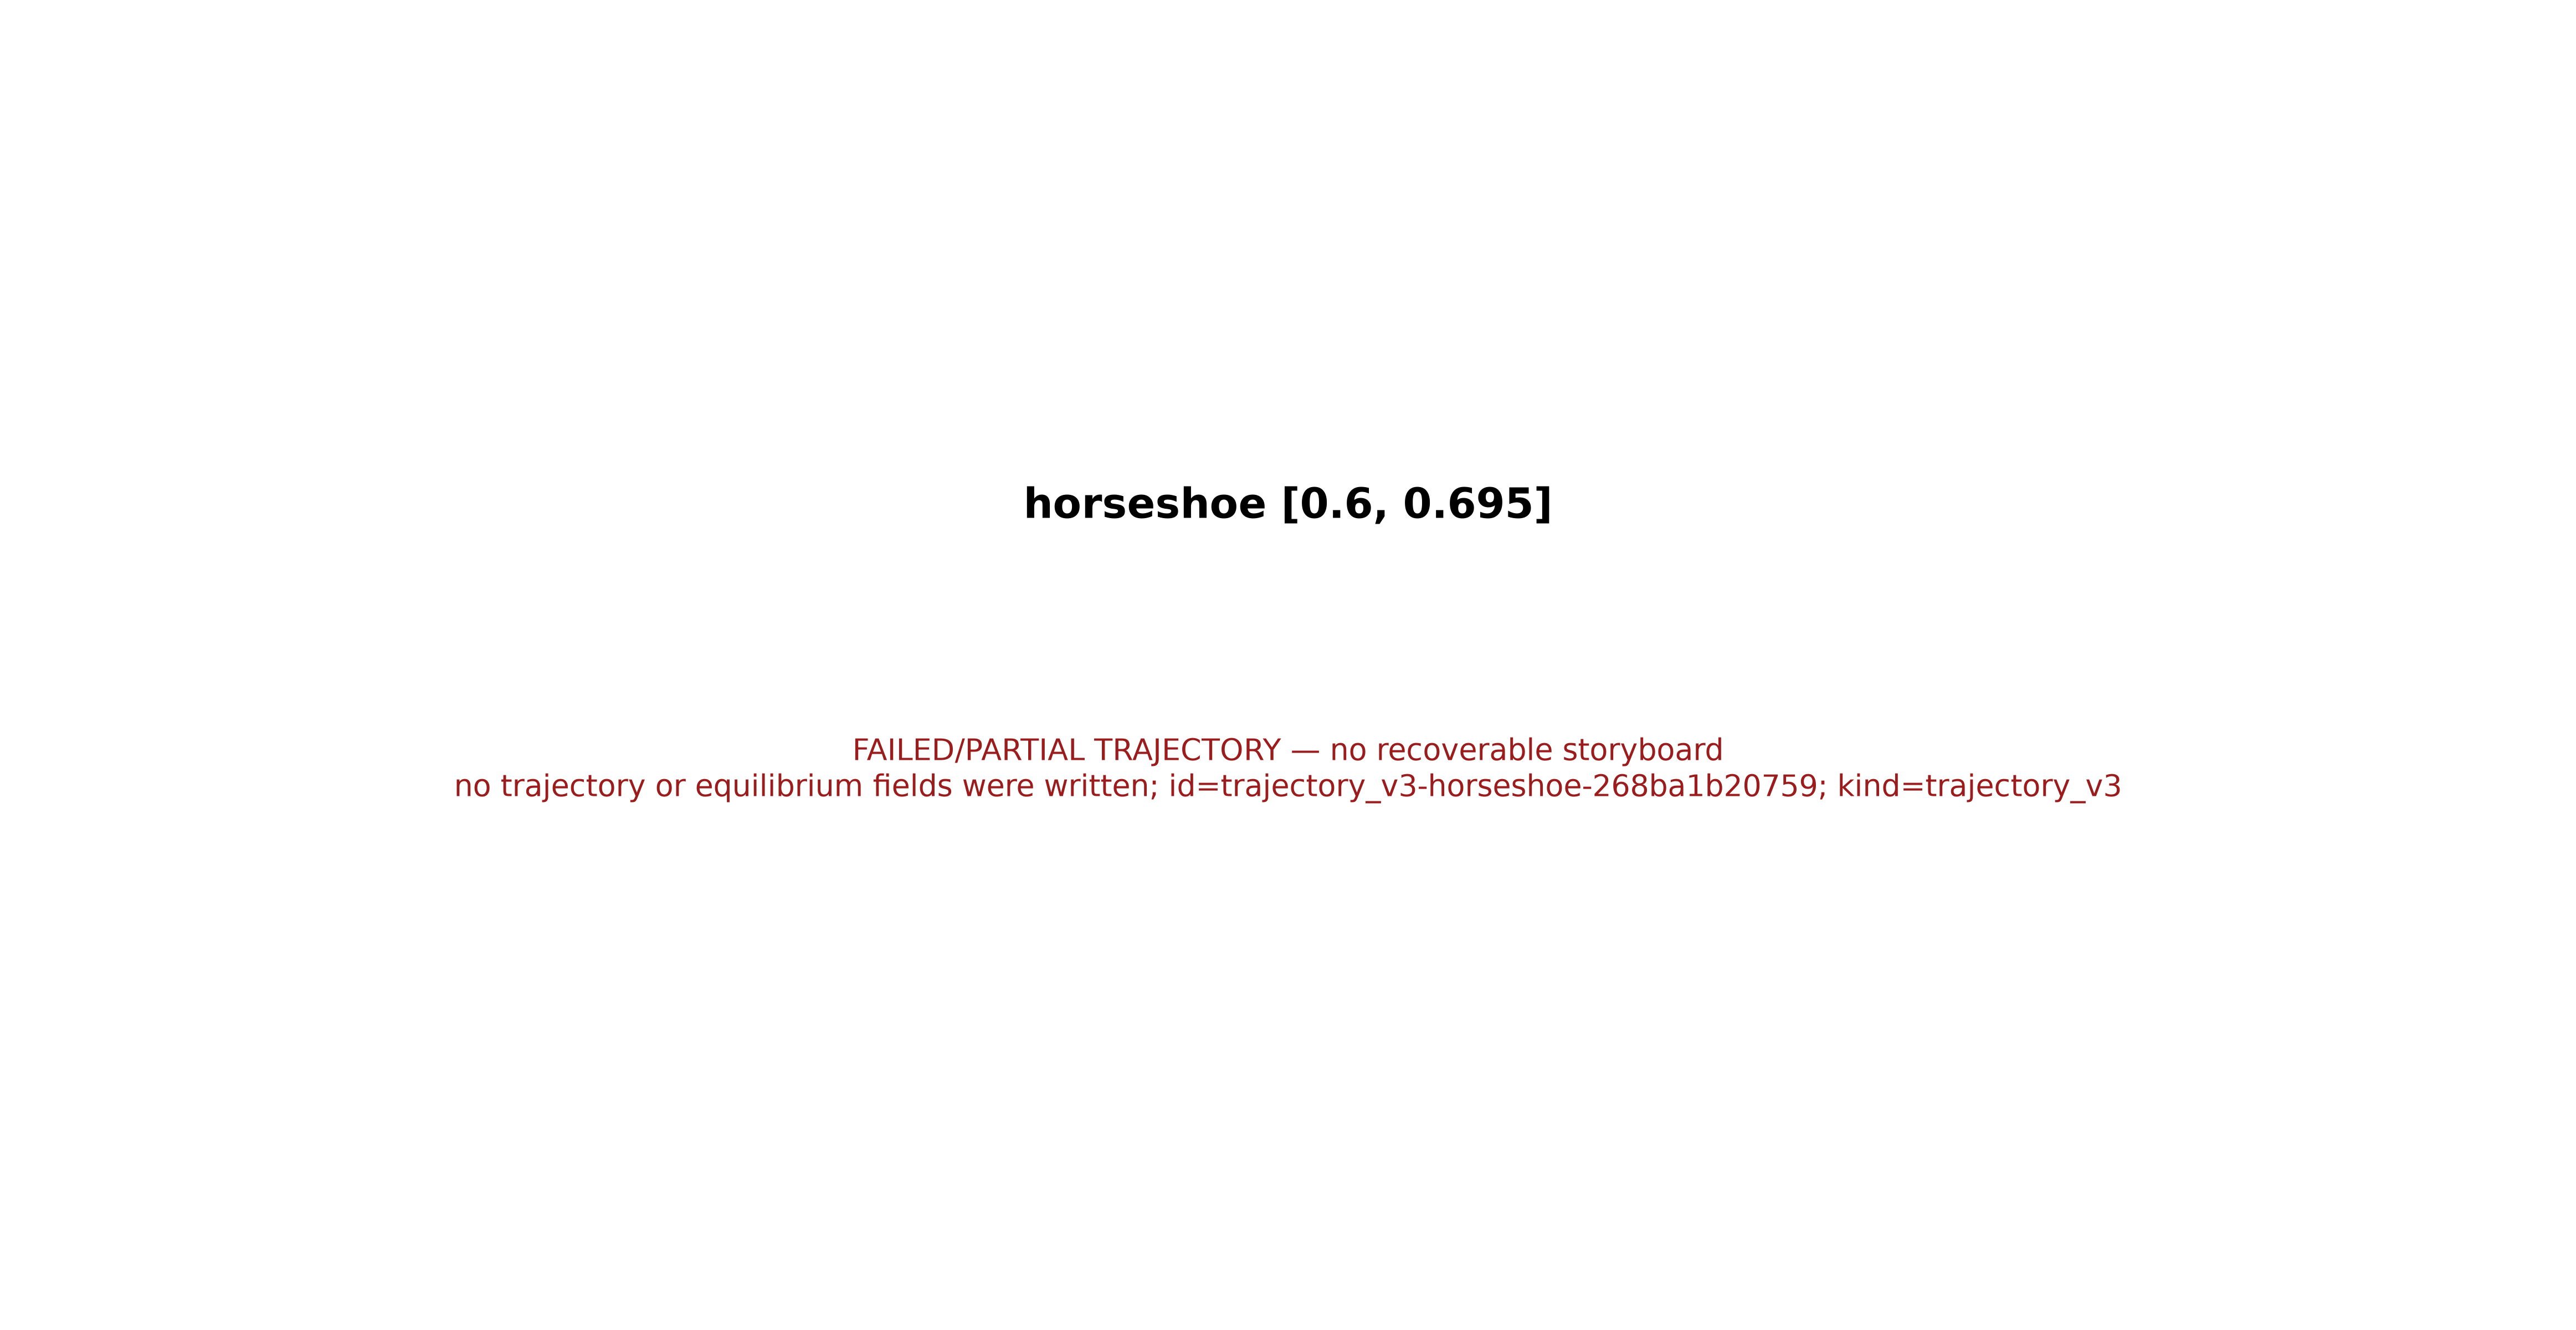
\includegraphics[width=0.88\linewidth]{figures/failed_band_evolution_039_horseshoe_0p6_0p695_trajectory_v3-horseshoe-268ba1b20759.png}
\caption{Supplemental failed/partial trajectory evidence for horseshoe at torsion levels $[0.6,0.695]$ (case trajectory\_v3-horseshoe-268ba1b20759; state=deferred; classification=deferred). The case is retained regardless of PDE or geometric success. Orange dashed curves are the fixed target band and blue solid curves are the moving equilibrium band; when state recovery is impossible, the PNG records the reason. Data status: diagnostic\_only.}
\label{fig:failed-storyboard-trajectory-v3-horseshoe-268ba1b20759}
\end{figure}

\begin{figure}[tbp]
\centering
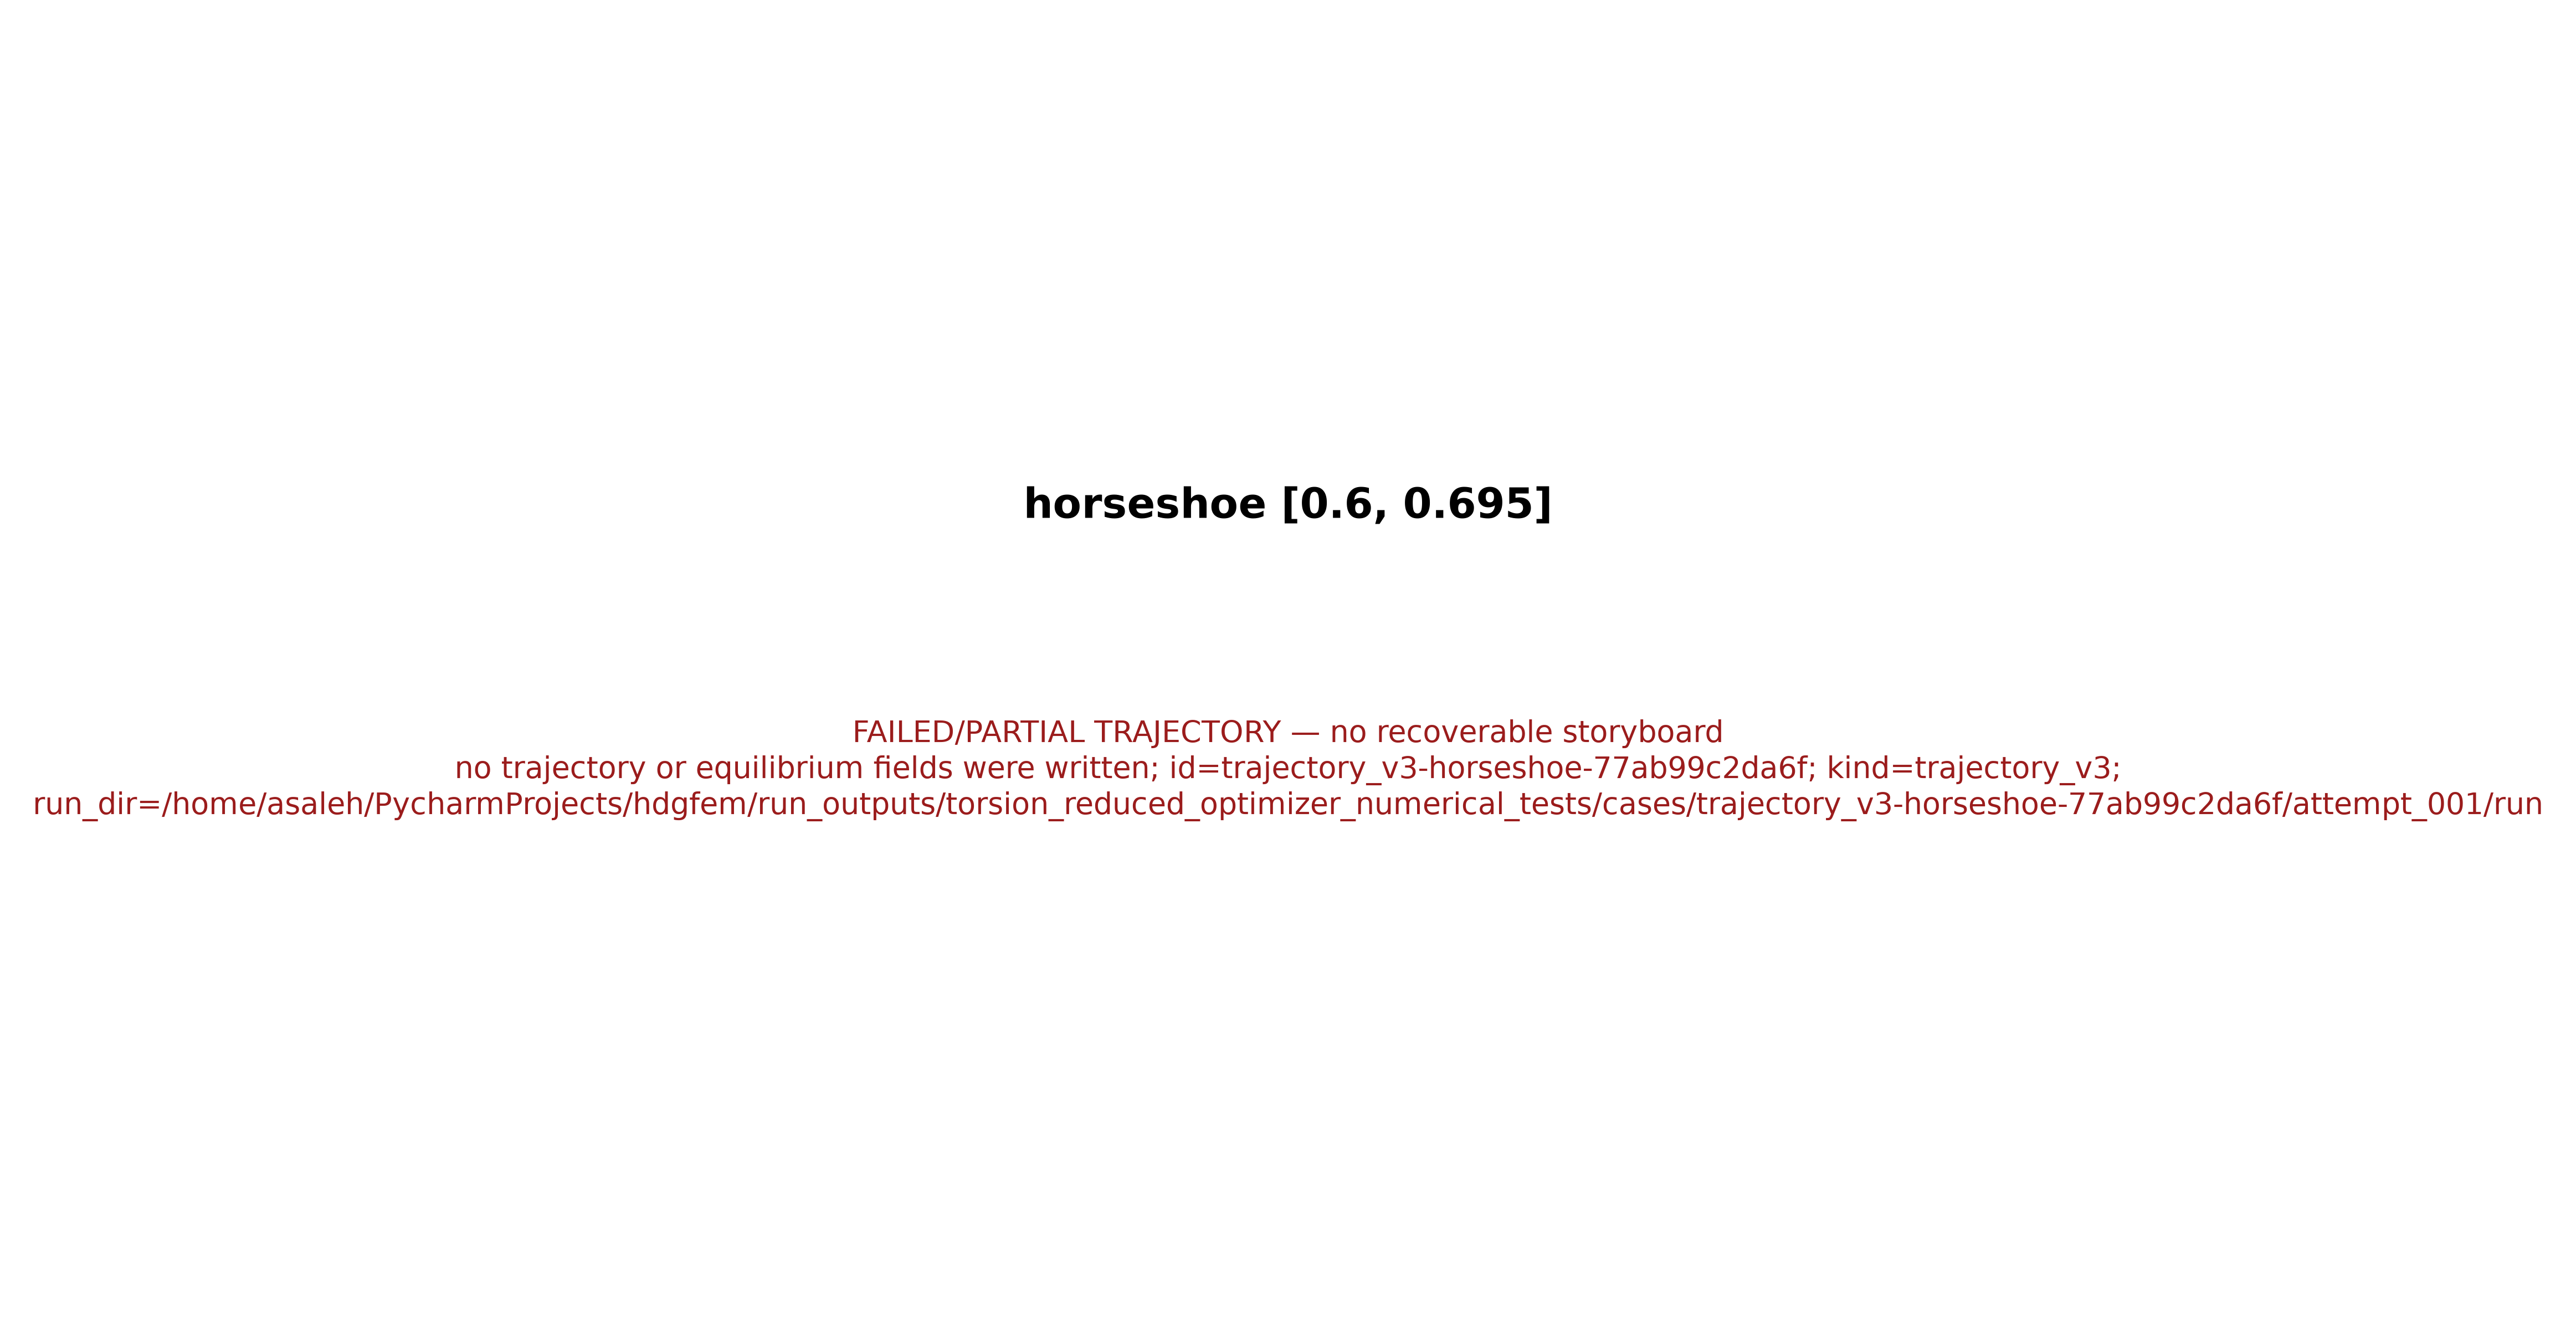
\includegraphics[width=0.88\linewidth]{figures/failed_band_evolution_040_horseshoe_0p6_0p695_trajectory_v3-horseshoe-77ab99c2da6f.png}
\caption{Supplemental failed/partial trajectory evidence for horseshoe at torsion levels $[0.6,0.695]$ (case trajectory\_v3-horseshoe-77ab99c2da6f; state=failed; classification=pde\_failure). The case is retained regardless of PDE or geometric success. Orange dashed curves are the fixed target band and blue solid curves are the moving equilibrium band; when state recovery is impossible, the PNG records the reason. Data status: diagnostic\_only.}
\label{fig:failed-storyboard-trajectory-v3-horseshoe-77ab99c2da6f}
\end{figure}

\begin{figure}[tbp]
\centering
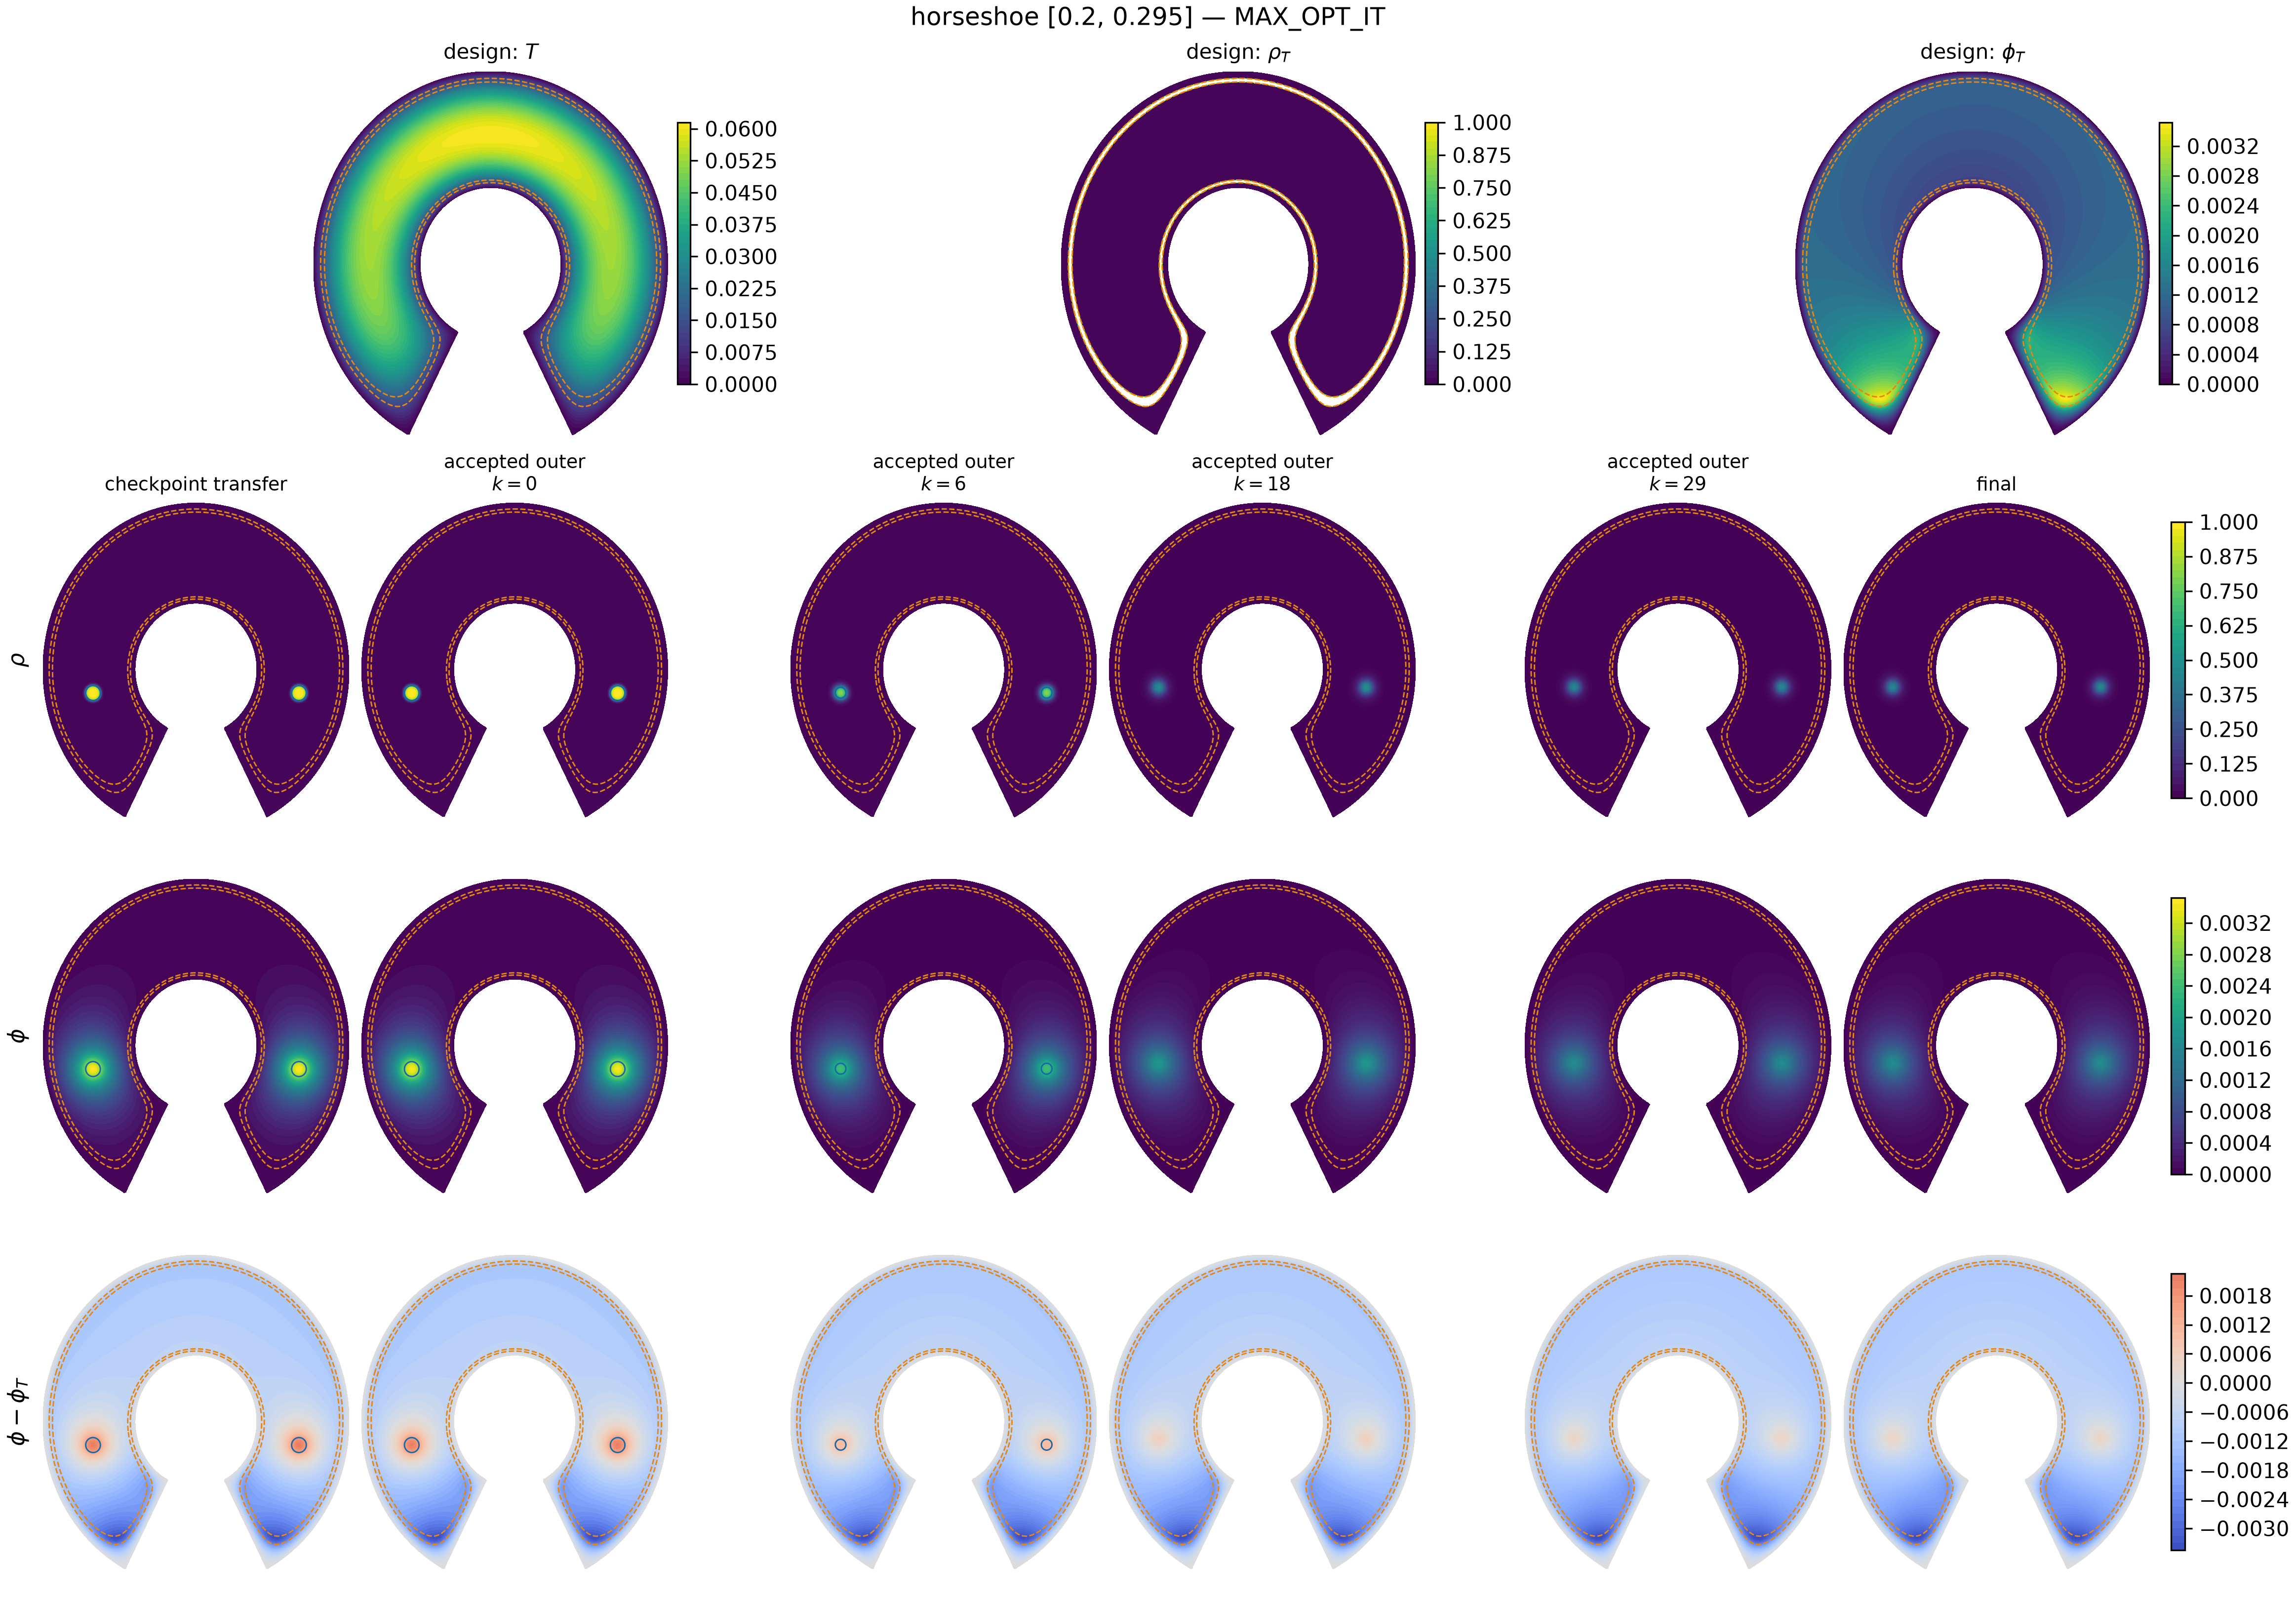
\includegraphics[width=0.88\linewidth]{figures/failed_band_evolution_041_horseshoe_0p2_0p295_trajectory_v3-horseshoe-b52bd3f19442.png}
\caption{Supplemental failed/partial trajectory evidence for horseshoe at torsion levels $[0.2,0.295]$ (case trajectory\_v3-horseshoe-b52bd3f19442; state=completed; classification=geometrically\_unsuccessful\_pde\_converged). The case is retained regardless of PDE or geometric success. Orange dashed curves are the fixed target band and blue solid curves are the moving equilibrium band; when state recovery is impossible, the PNG records the reason. Data status: actual.}
\label{fig:failed-storyboard-trajectory-v3-horseshoe-b52bd3f19442}
\end{figure}

\begin{figure}[tbp]
\centering
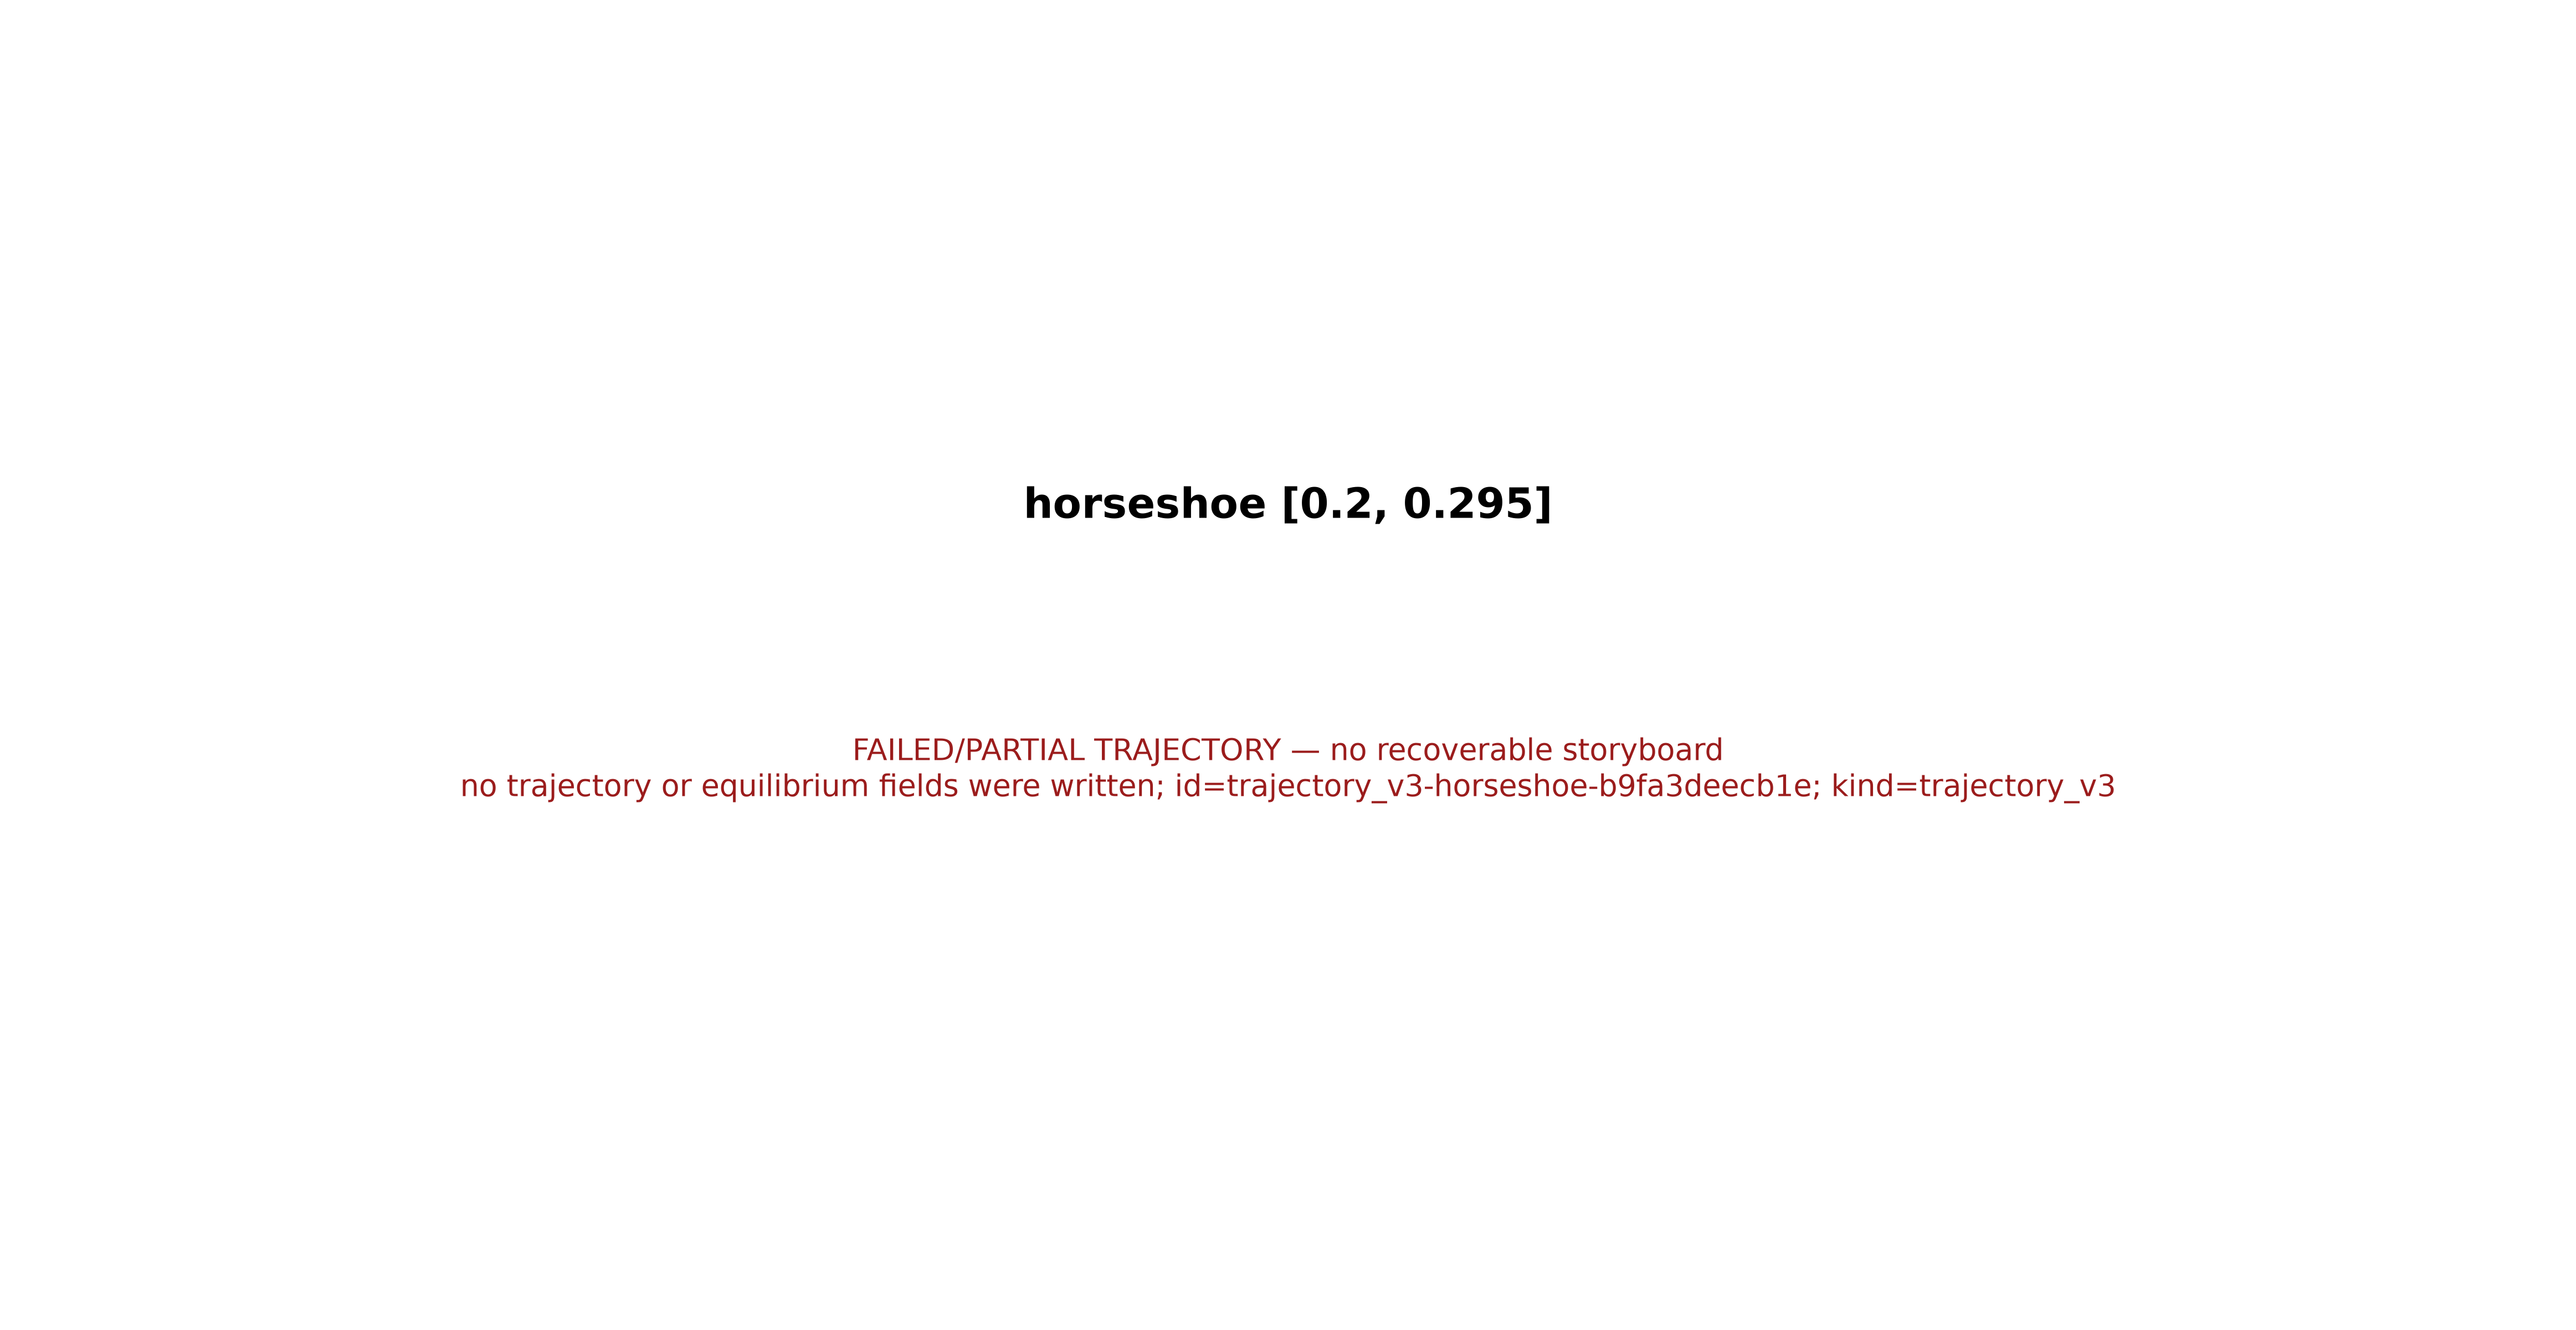
\includegraphics[width=0.88\linewidth]{figures/failed_band_evolution_042_horseshoe_0p2_0p295_trajectory_v3-horseshoe-b9fa3deecb1e.png}
\caption{Supplemental failed/partial trajectory evidence for horseshoe at torsion levels $[0.2,0.295]$ (case trajectory\_v3-horseshoe-b9fa3deecb1e; state=deferred; classification=deferred). The case is retained regardless of PDE or geometric success. Orange dashed curves are the fixed target band and blue solid curves are the moving equilibrium band; when state recovery is impossible, the PNG records the reason. Data status: diagnostic\_only.}
\label{fig:failed-storyboard-trajectory-v3-horseshoe-b9fa3deecb1e}
\end{figure}

\begin{figure}[tbp]
\centering
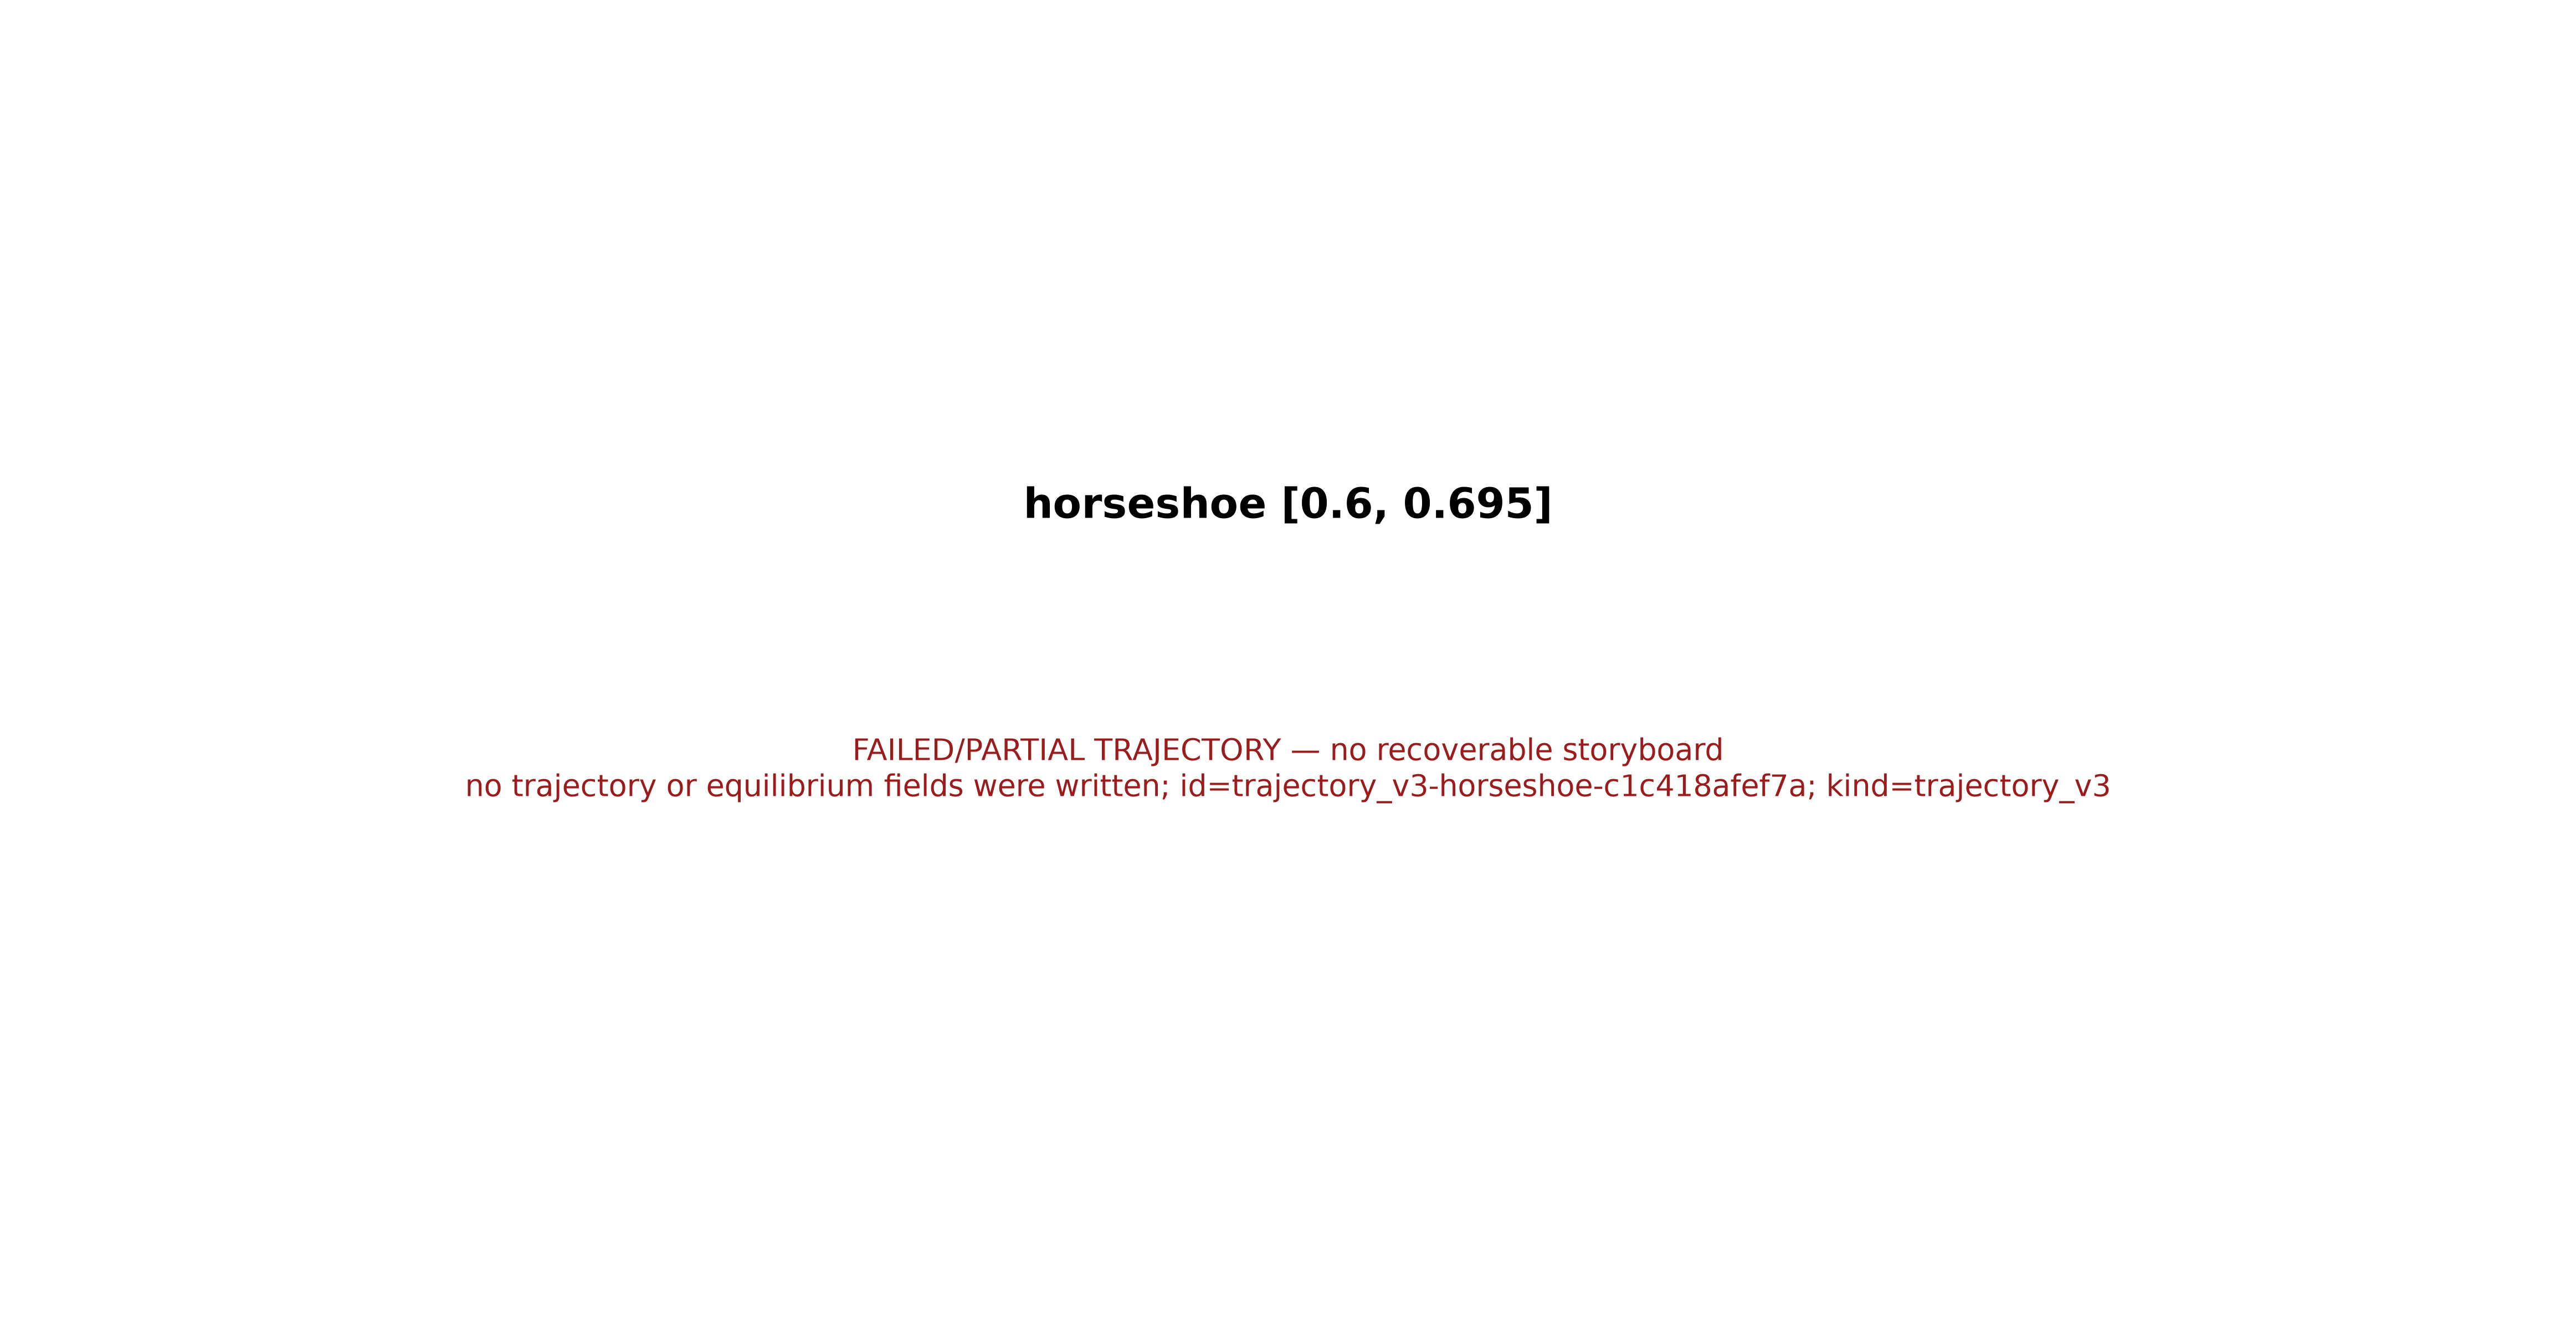
\includegraphics[width=0.88\linewidth]{figures/failed_band_evolution_043_horseshoe_0p6_0p695_trajectory_v3-horseshoe-c1c418afef7a.png}
\caption{Supplemental failed/partial trajectory evidence for horseshoe at torsion levels $[0.6,0.695]$ (case trajectory\_v3-horseshoe-c1c418afef7a; state=deferred; classification=deferred). The case is retained regardless of PDE or geometric success. Orange dashed curves are the fixed target band and blue solid curves are the moving equilibrium band; when state recovery is impossible, the PNG records the reason. Data status: diagnostic\_only.}
\label{fig:failed-storyboard-trajectory-v3-horseshoe-c1c418afef7a}
\end{figure}

\begin{figure}[tbp]
\centering
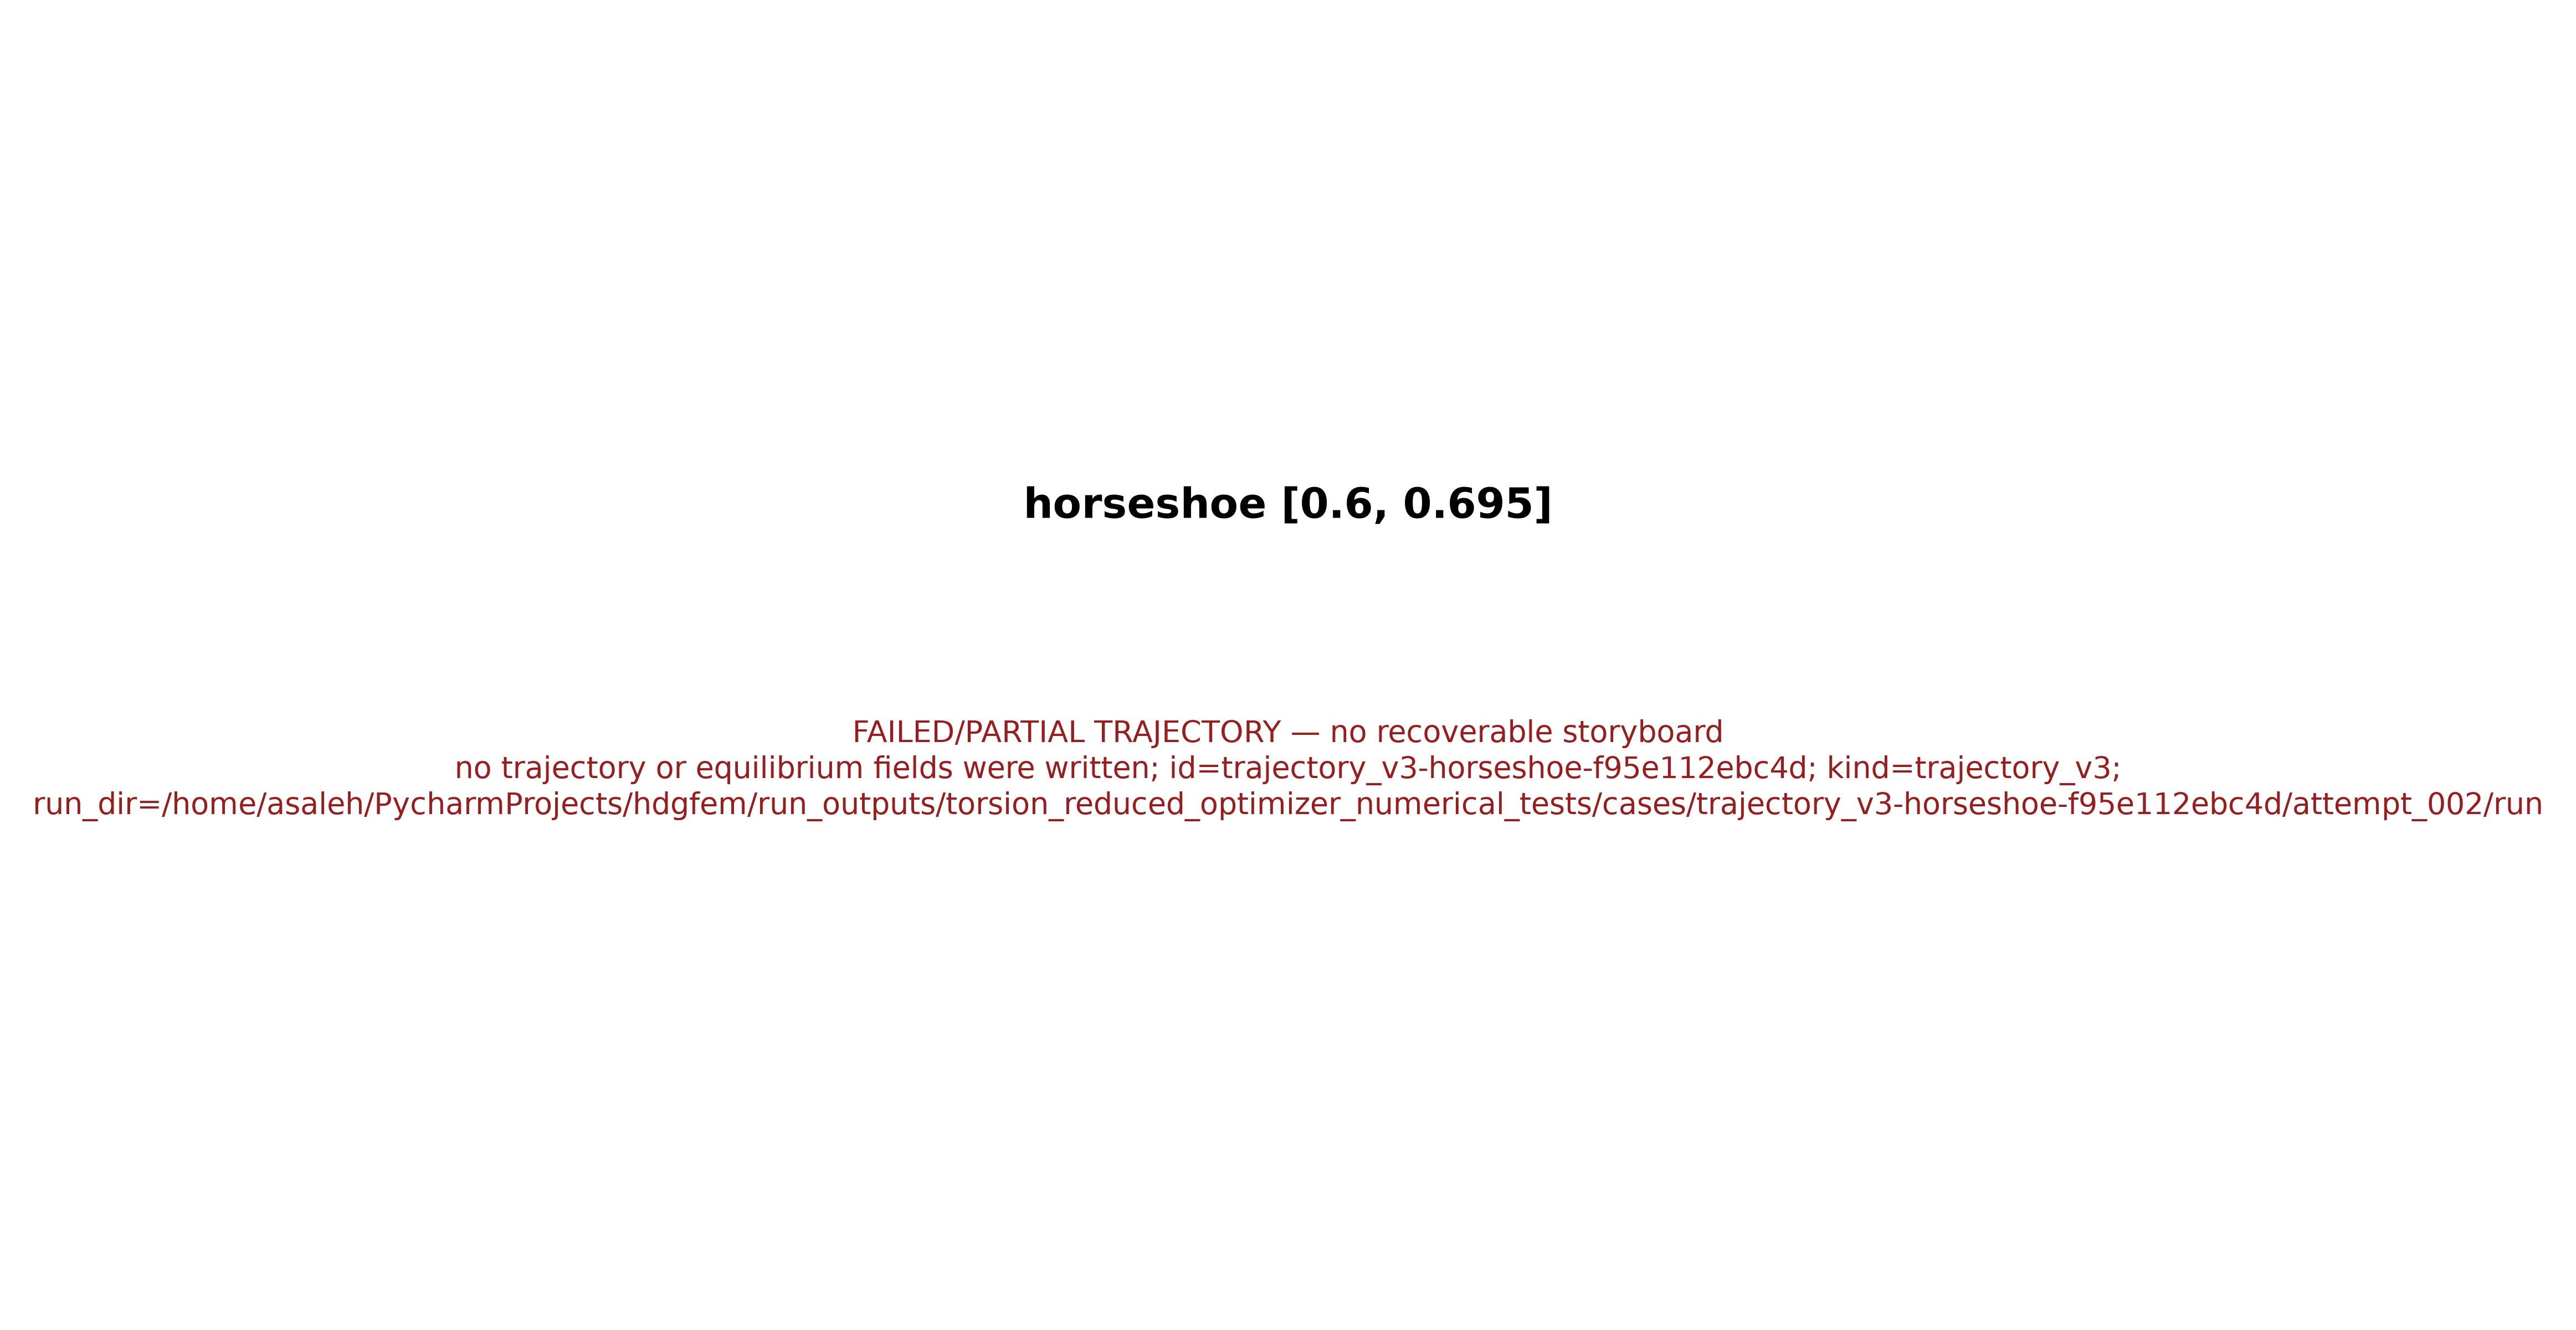
\includegraphics[width=0.88\linewidth]{figures/failed_band_evolution_044_horseshoe_0p6_0p695_trajectory_v3-horseshoe-f95e112ebc4d.png}
\caption{Supplemental failed/partial trajectory evidence for horseshoe at torsion levels $[0.6,0.695]$ (case trajectory\_v3-horseshoe-f95e112ebc4d; state=failed; classification=pde\_failure). The case is retained regardless of PDE or geometric success. Orange dashed curves are the fixed target band and blue solid curves are the moving equilibrium band; when state recovery is impossible, the PNG records the reason. Data status: diagnostic\_only.}
\label{fig:failed-storyboard-trajectory-v3-horseshoe-f95e112ebc4d}
\end{figure}

\begin{figure}[tbp]
\centering
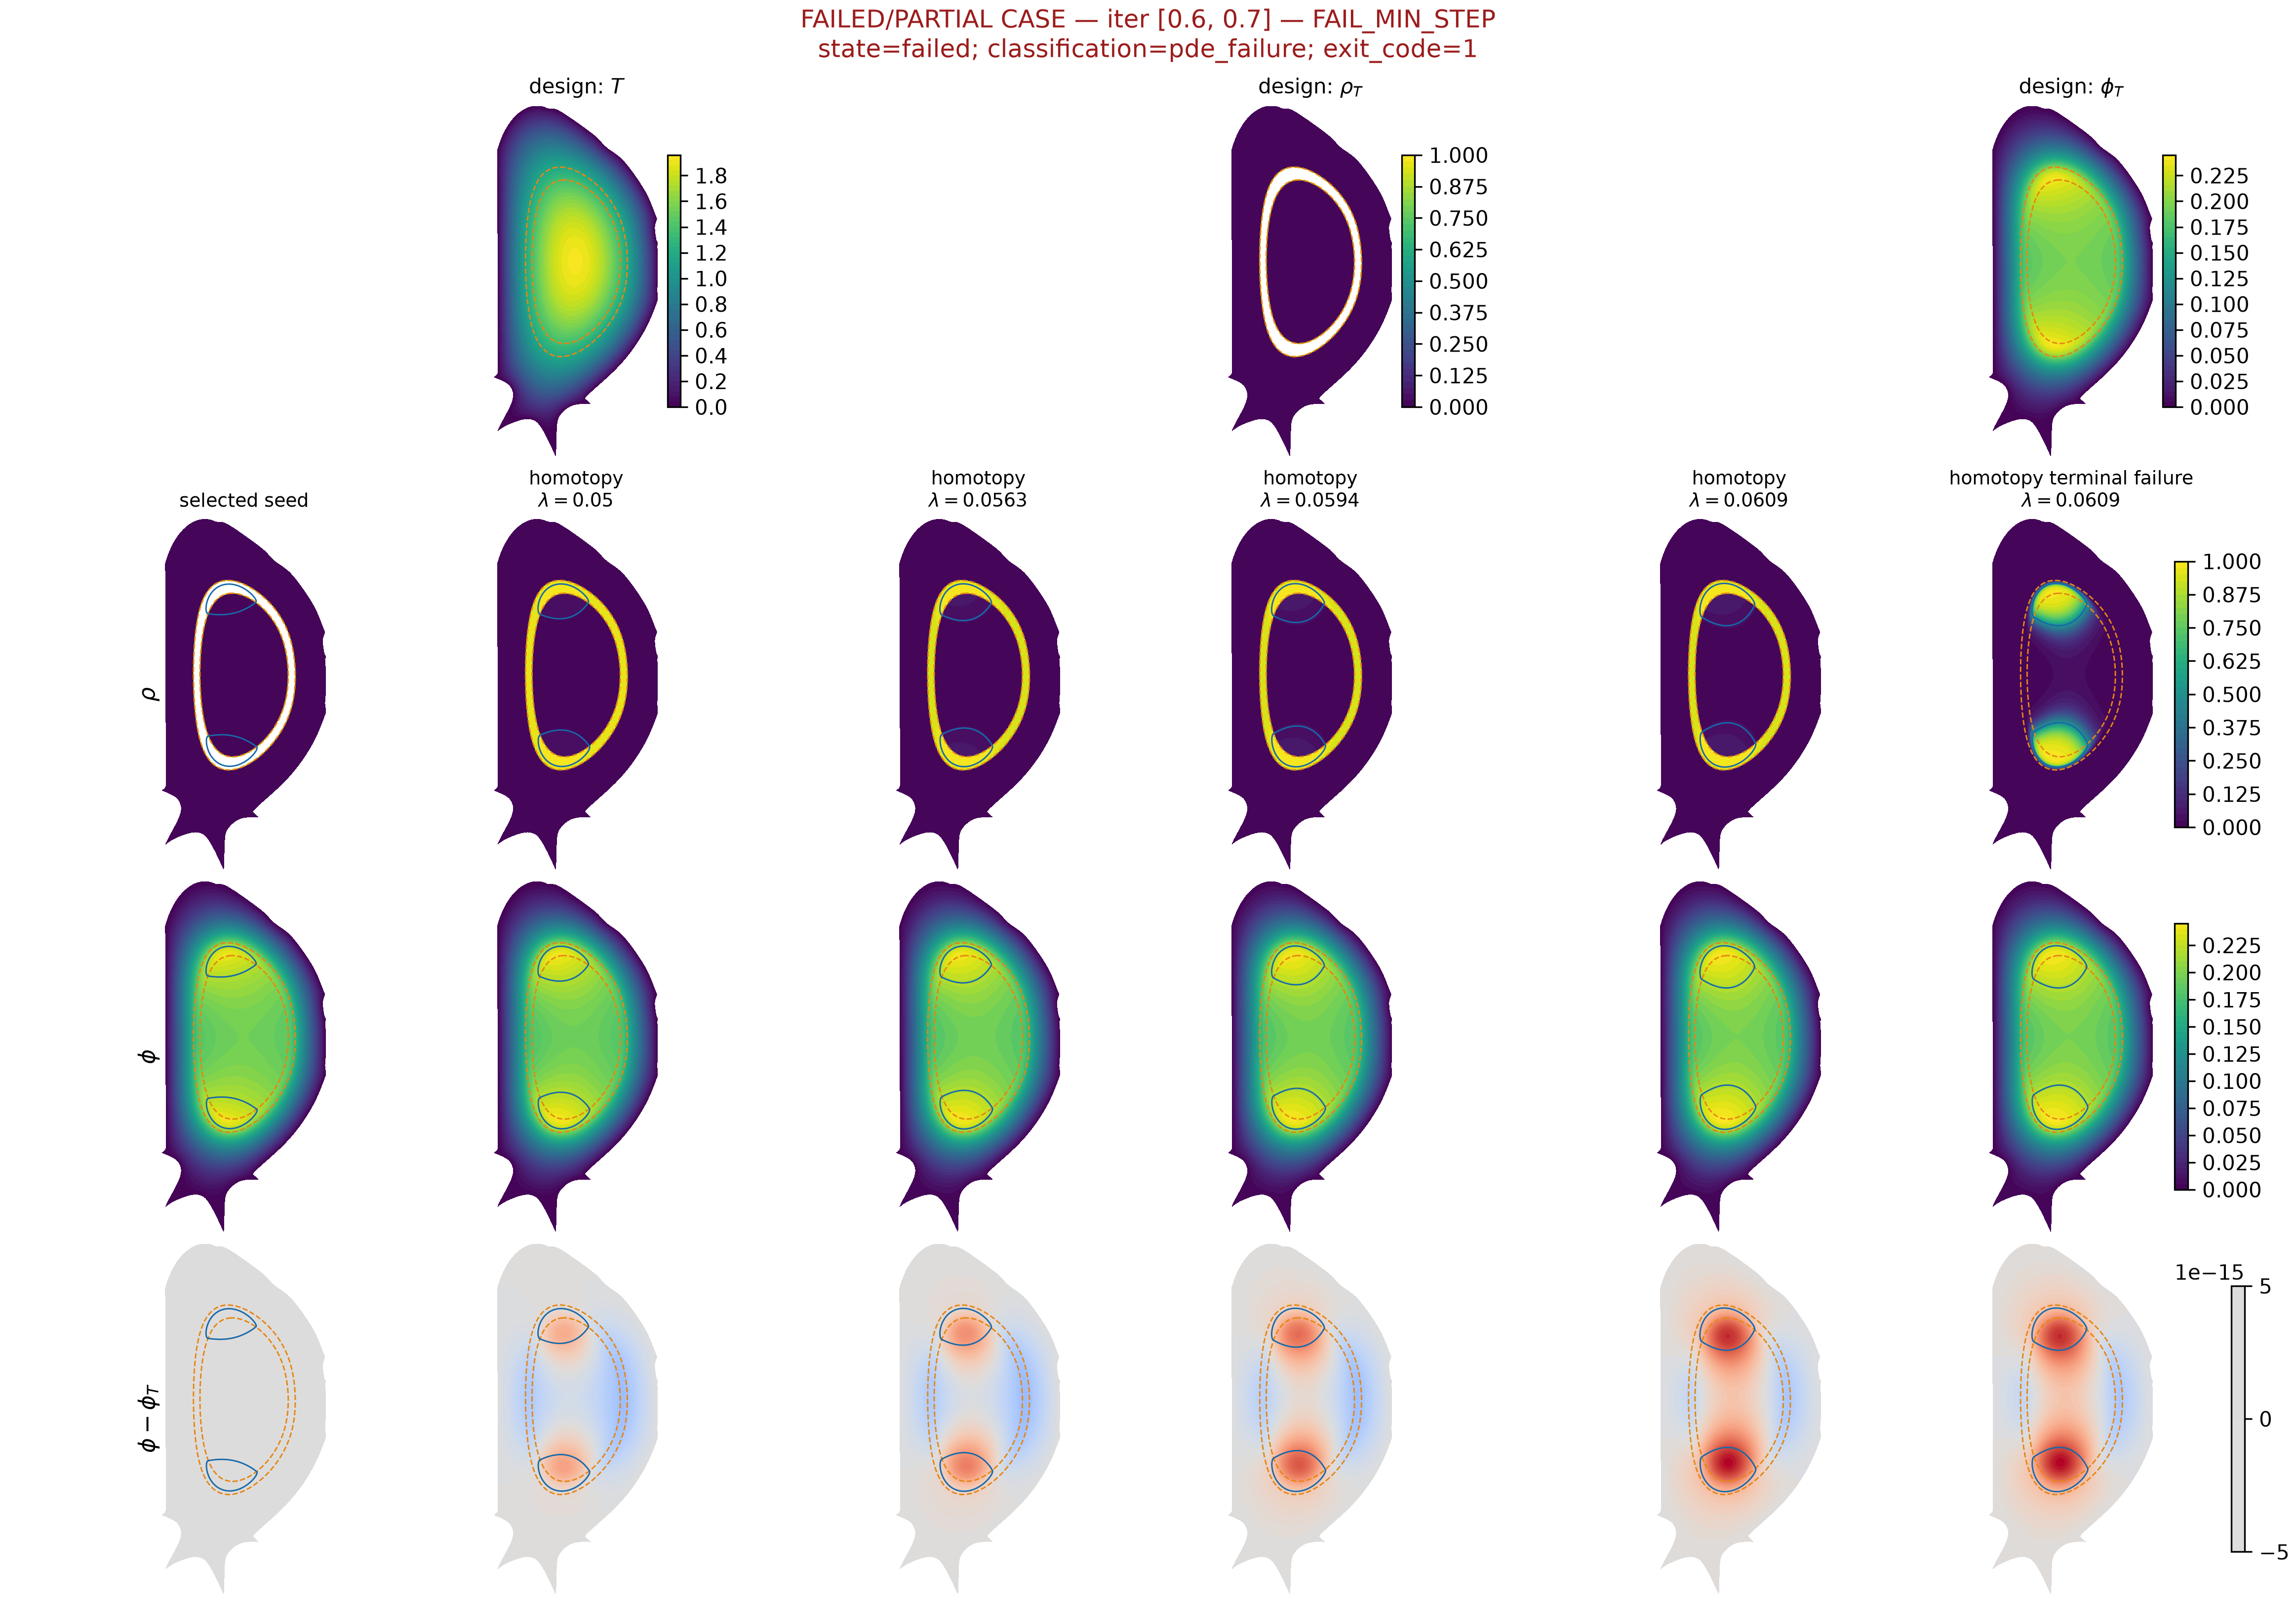
\includegraphics[width=0.88\linewidth]{figures/failed_band_evolution_045_iter_0p6_0p7_trajectory-iter-ef35b47caeda.png}
\caption{Supplemental failed/partial trajectory evidence for iter at torsion levels $[0.6,0.7]$ (case trajectory-iter-ef35b47caeda; state=failed; classification=pde\_failure). The case is retained regardless of PDE or geometric success. Orange dashed curves are the fixed target band and blue solid curves are the moving equilibrium band; when state recovery is impossible, the PNG records the reason. Data status: actual.}
\label{fig:failed-storyboard-trajectory-iter-ef35b47caeda}
\end{figure}

\clearpage

\begin{figure}[tbp]
\centering
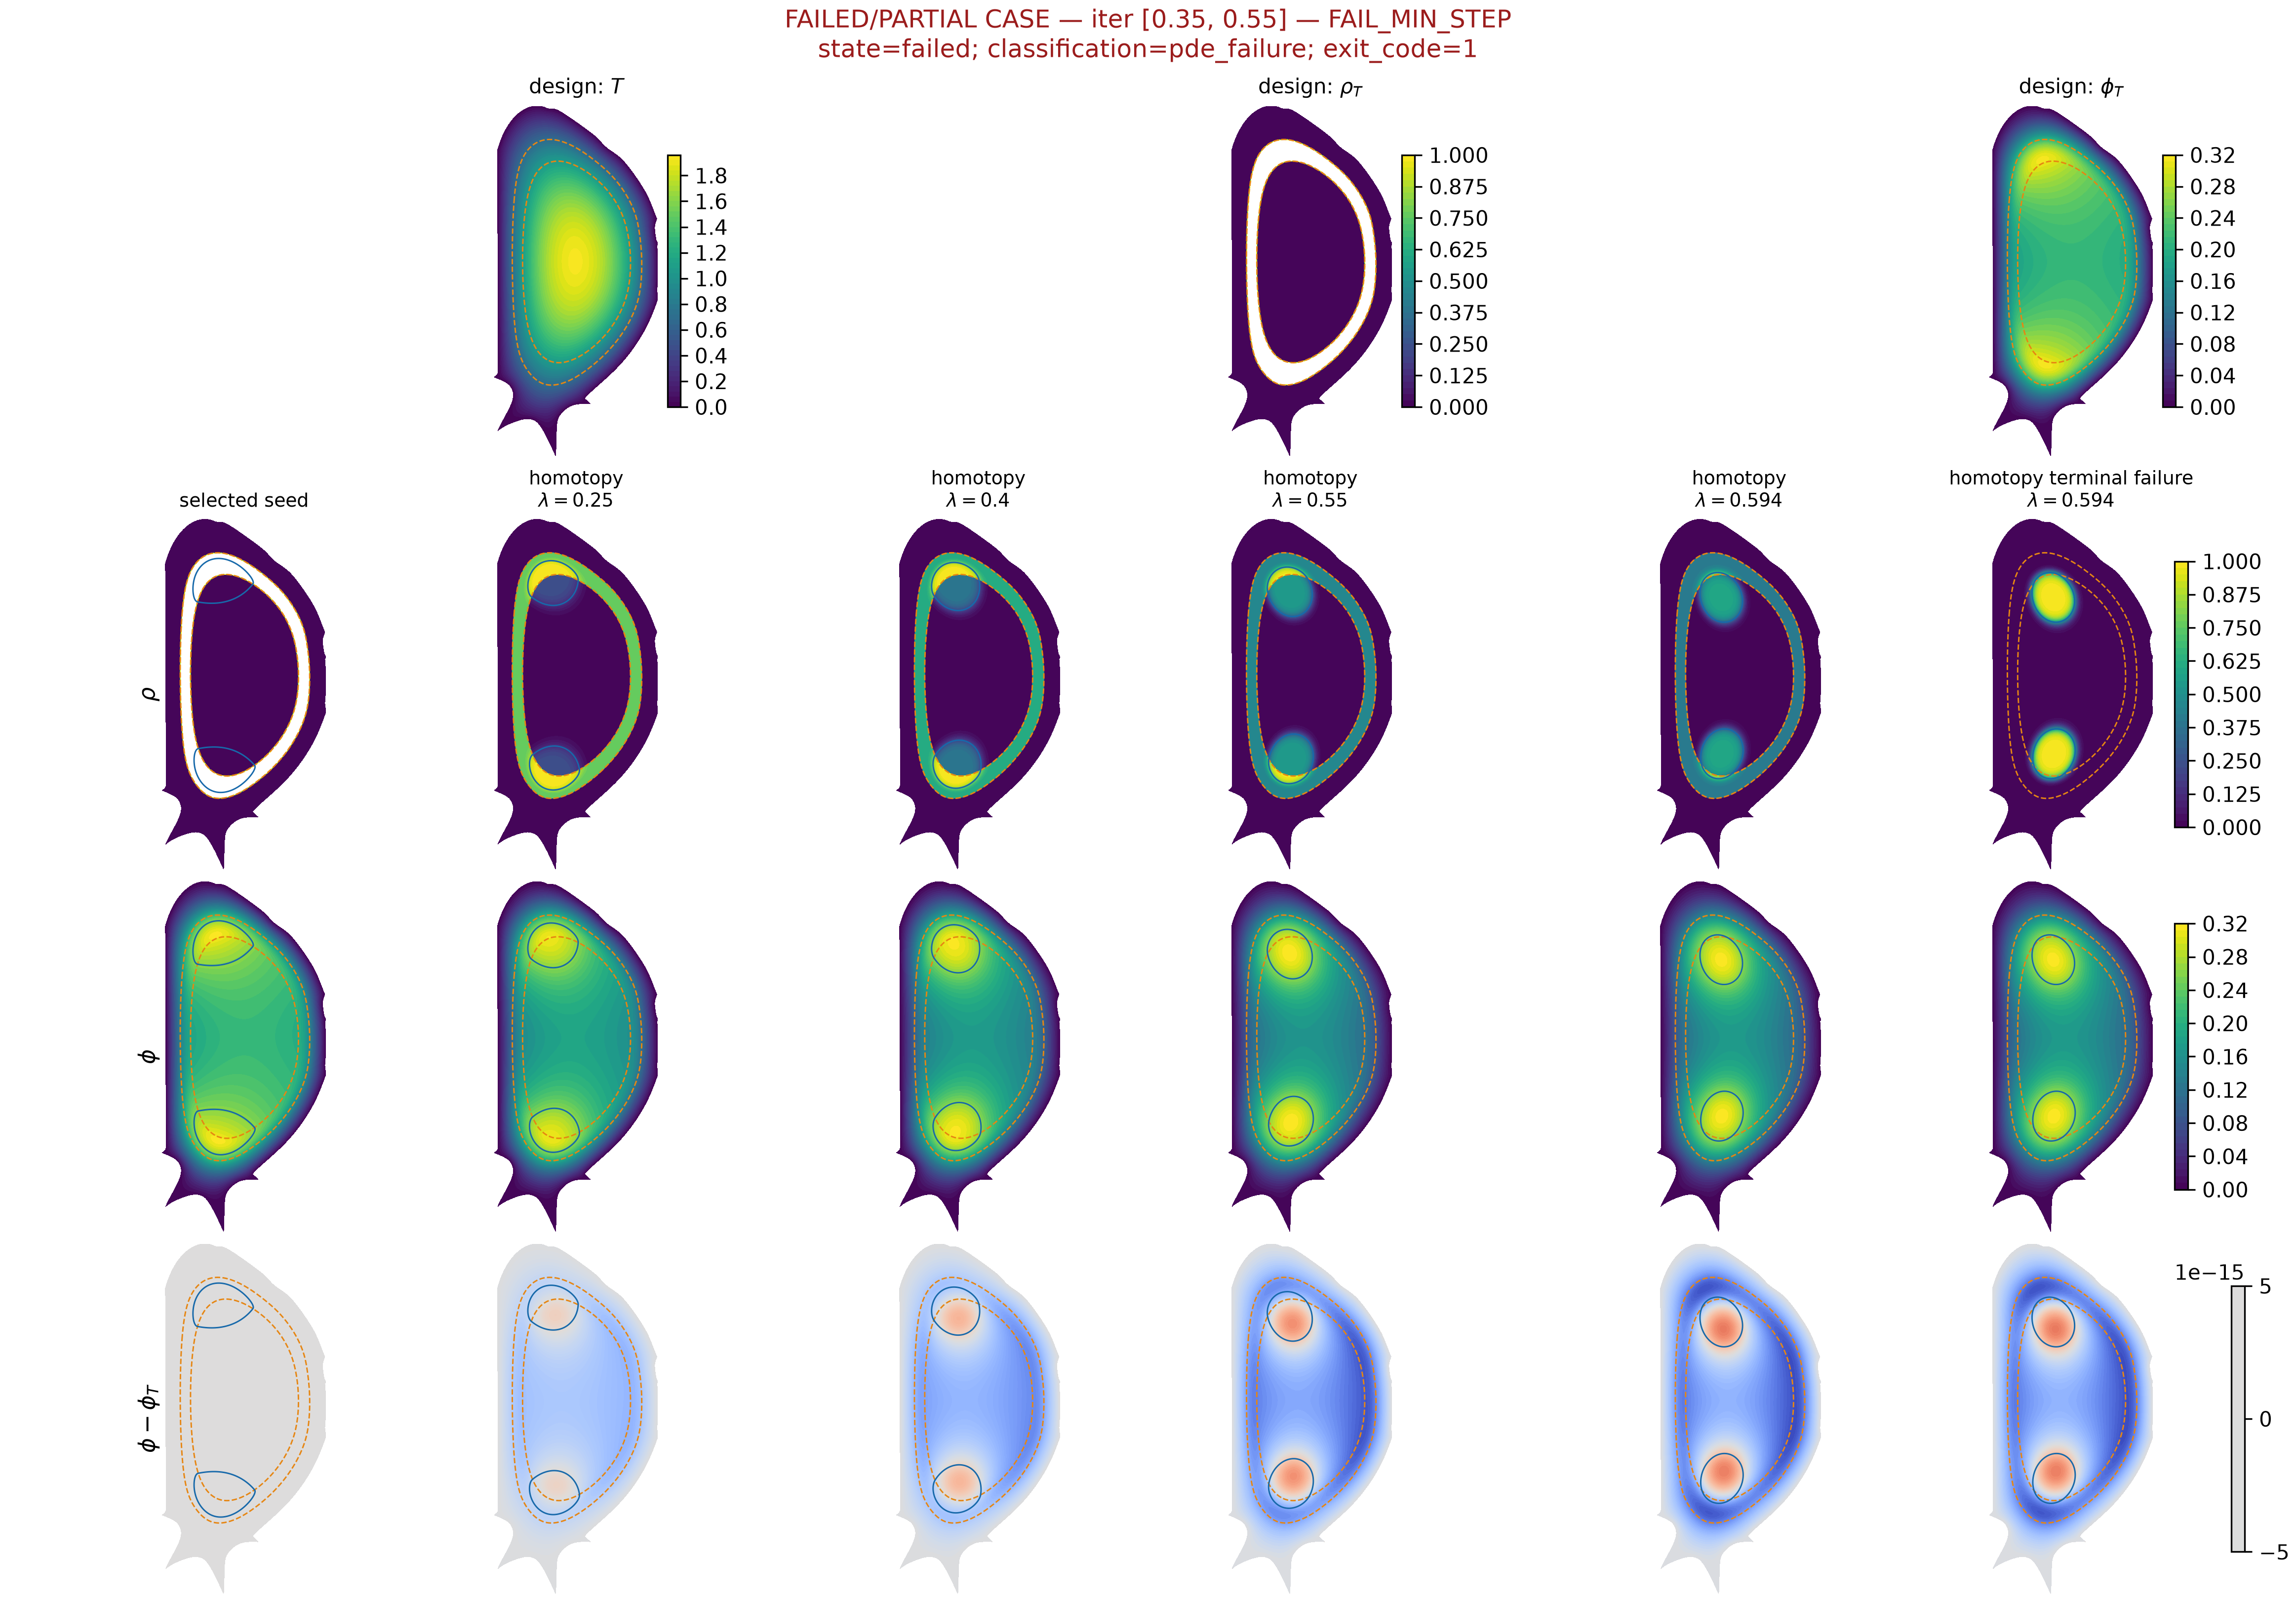
\includegraphics[width=0.88\linewidth]{figures/failed_band_evolution_046_iter_0p35_0p55_trajectory_candidate-iter-9a9d9ae4682b.png}
\caption{Supplemental failed/partial trajectory evidence for iter at torsion levels $[0.35,0.55]$ (case trajectory\_candidate-iter-9a9d9ae4682b; state=failed; classification=pde\_failure). The case is retained regardless of PDE or geometric success. Orange dashed curves are the fixed target band and blue solid curves are the moving equilibrium band; when state recovery is impossible, the PNG records the reason. Data status: actual.}
\label{fig:failed-storyboard-trajectory-candidate-iter-9a9d9ae4682b}
\end{figure}

\begin{figure}[tbp]
\centering
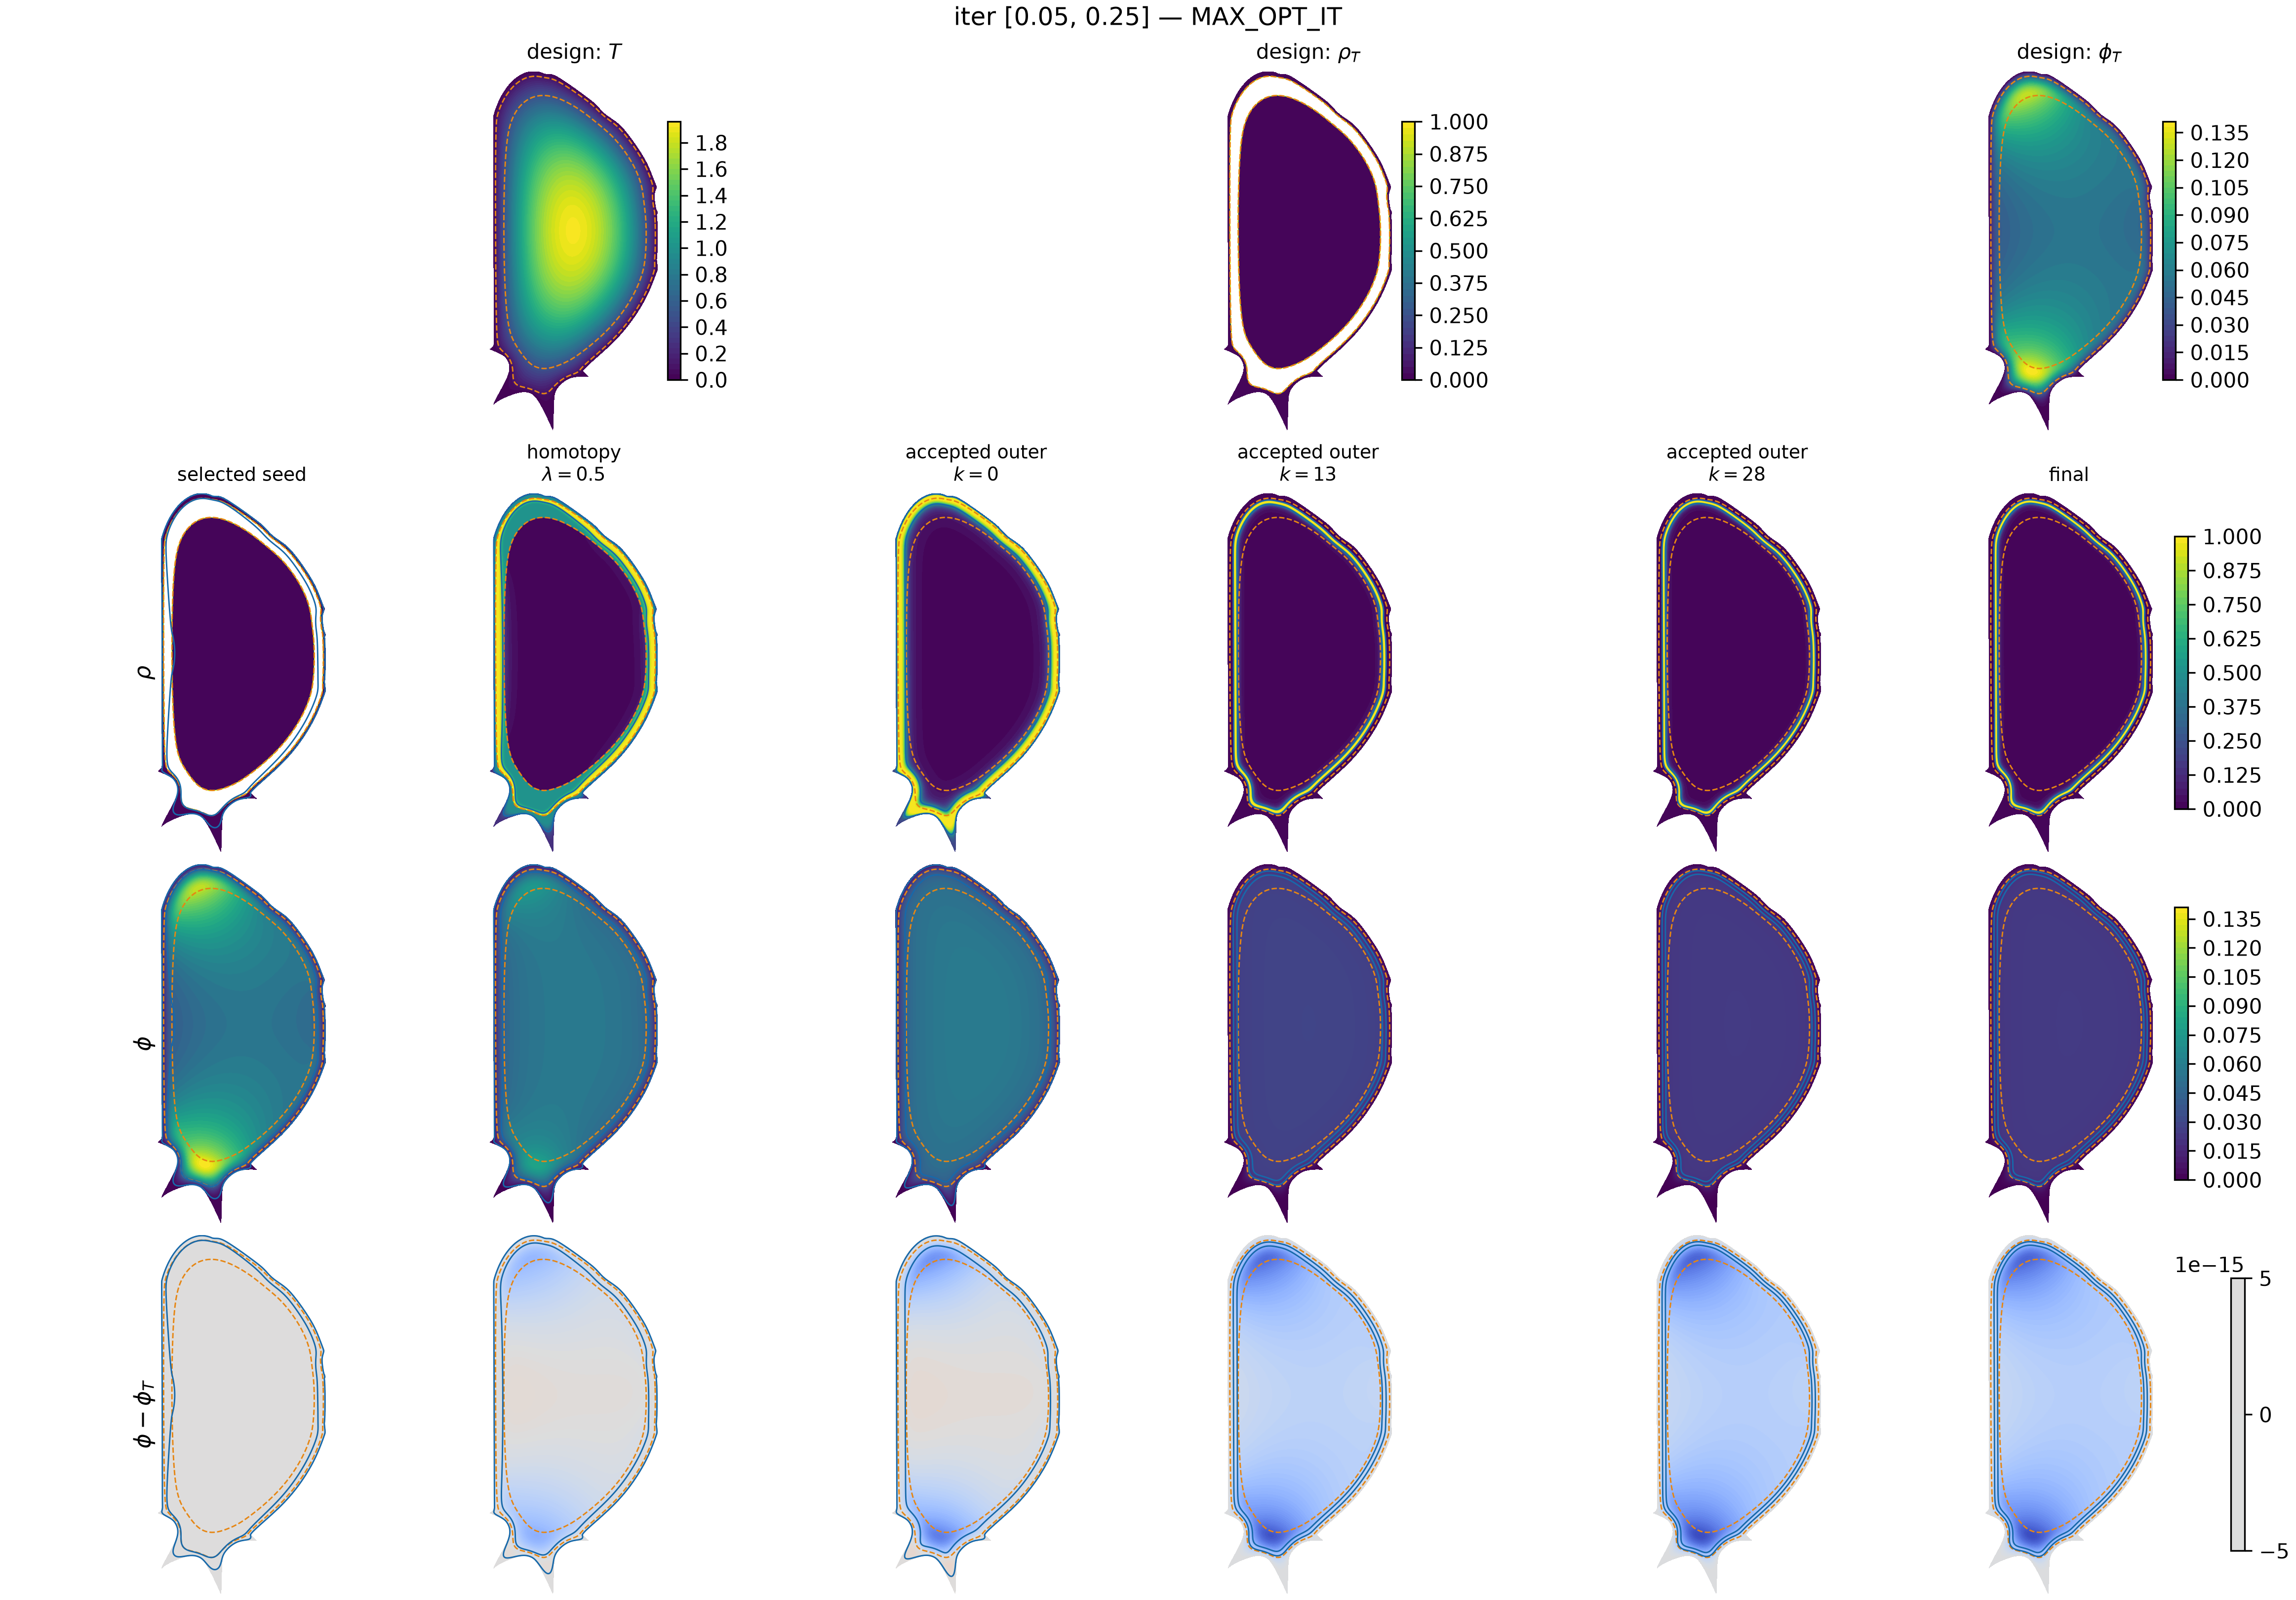
\includegraphics[width=0.88\linewidth]{figures/failed_band_evolution_047_iter_0p05_0p25_trajectory_candidate-iter-9aecf30783ce.png}
\caption{Supplemental failed/partial trajectory evidence for iter at torsion levels $[0.05,0.25]$ (case trajectory\_candidate-iter-9aecf30783ce; state=completed; classification=pde\_converged\_with\_capped\_trials). The case is retained regardless of PDE or geometric success. Orange dashed curves are the fixed target band and blue solid curves are the moving equilibrium band; when state recovery is impossible, the PNG records the reason. Data status: actual.}
\label{fig:failed-storyboard-trajectory-candidate-iter-9aecf30783ce}
\end{figure}

\begin{figure}[tbp]
\centering
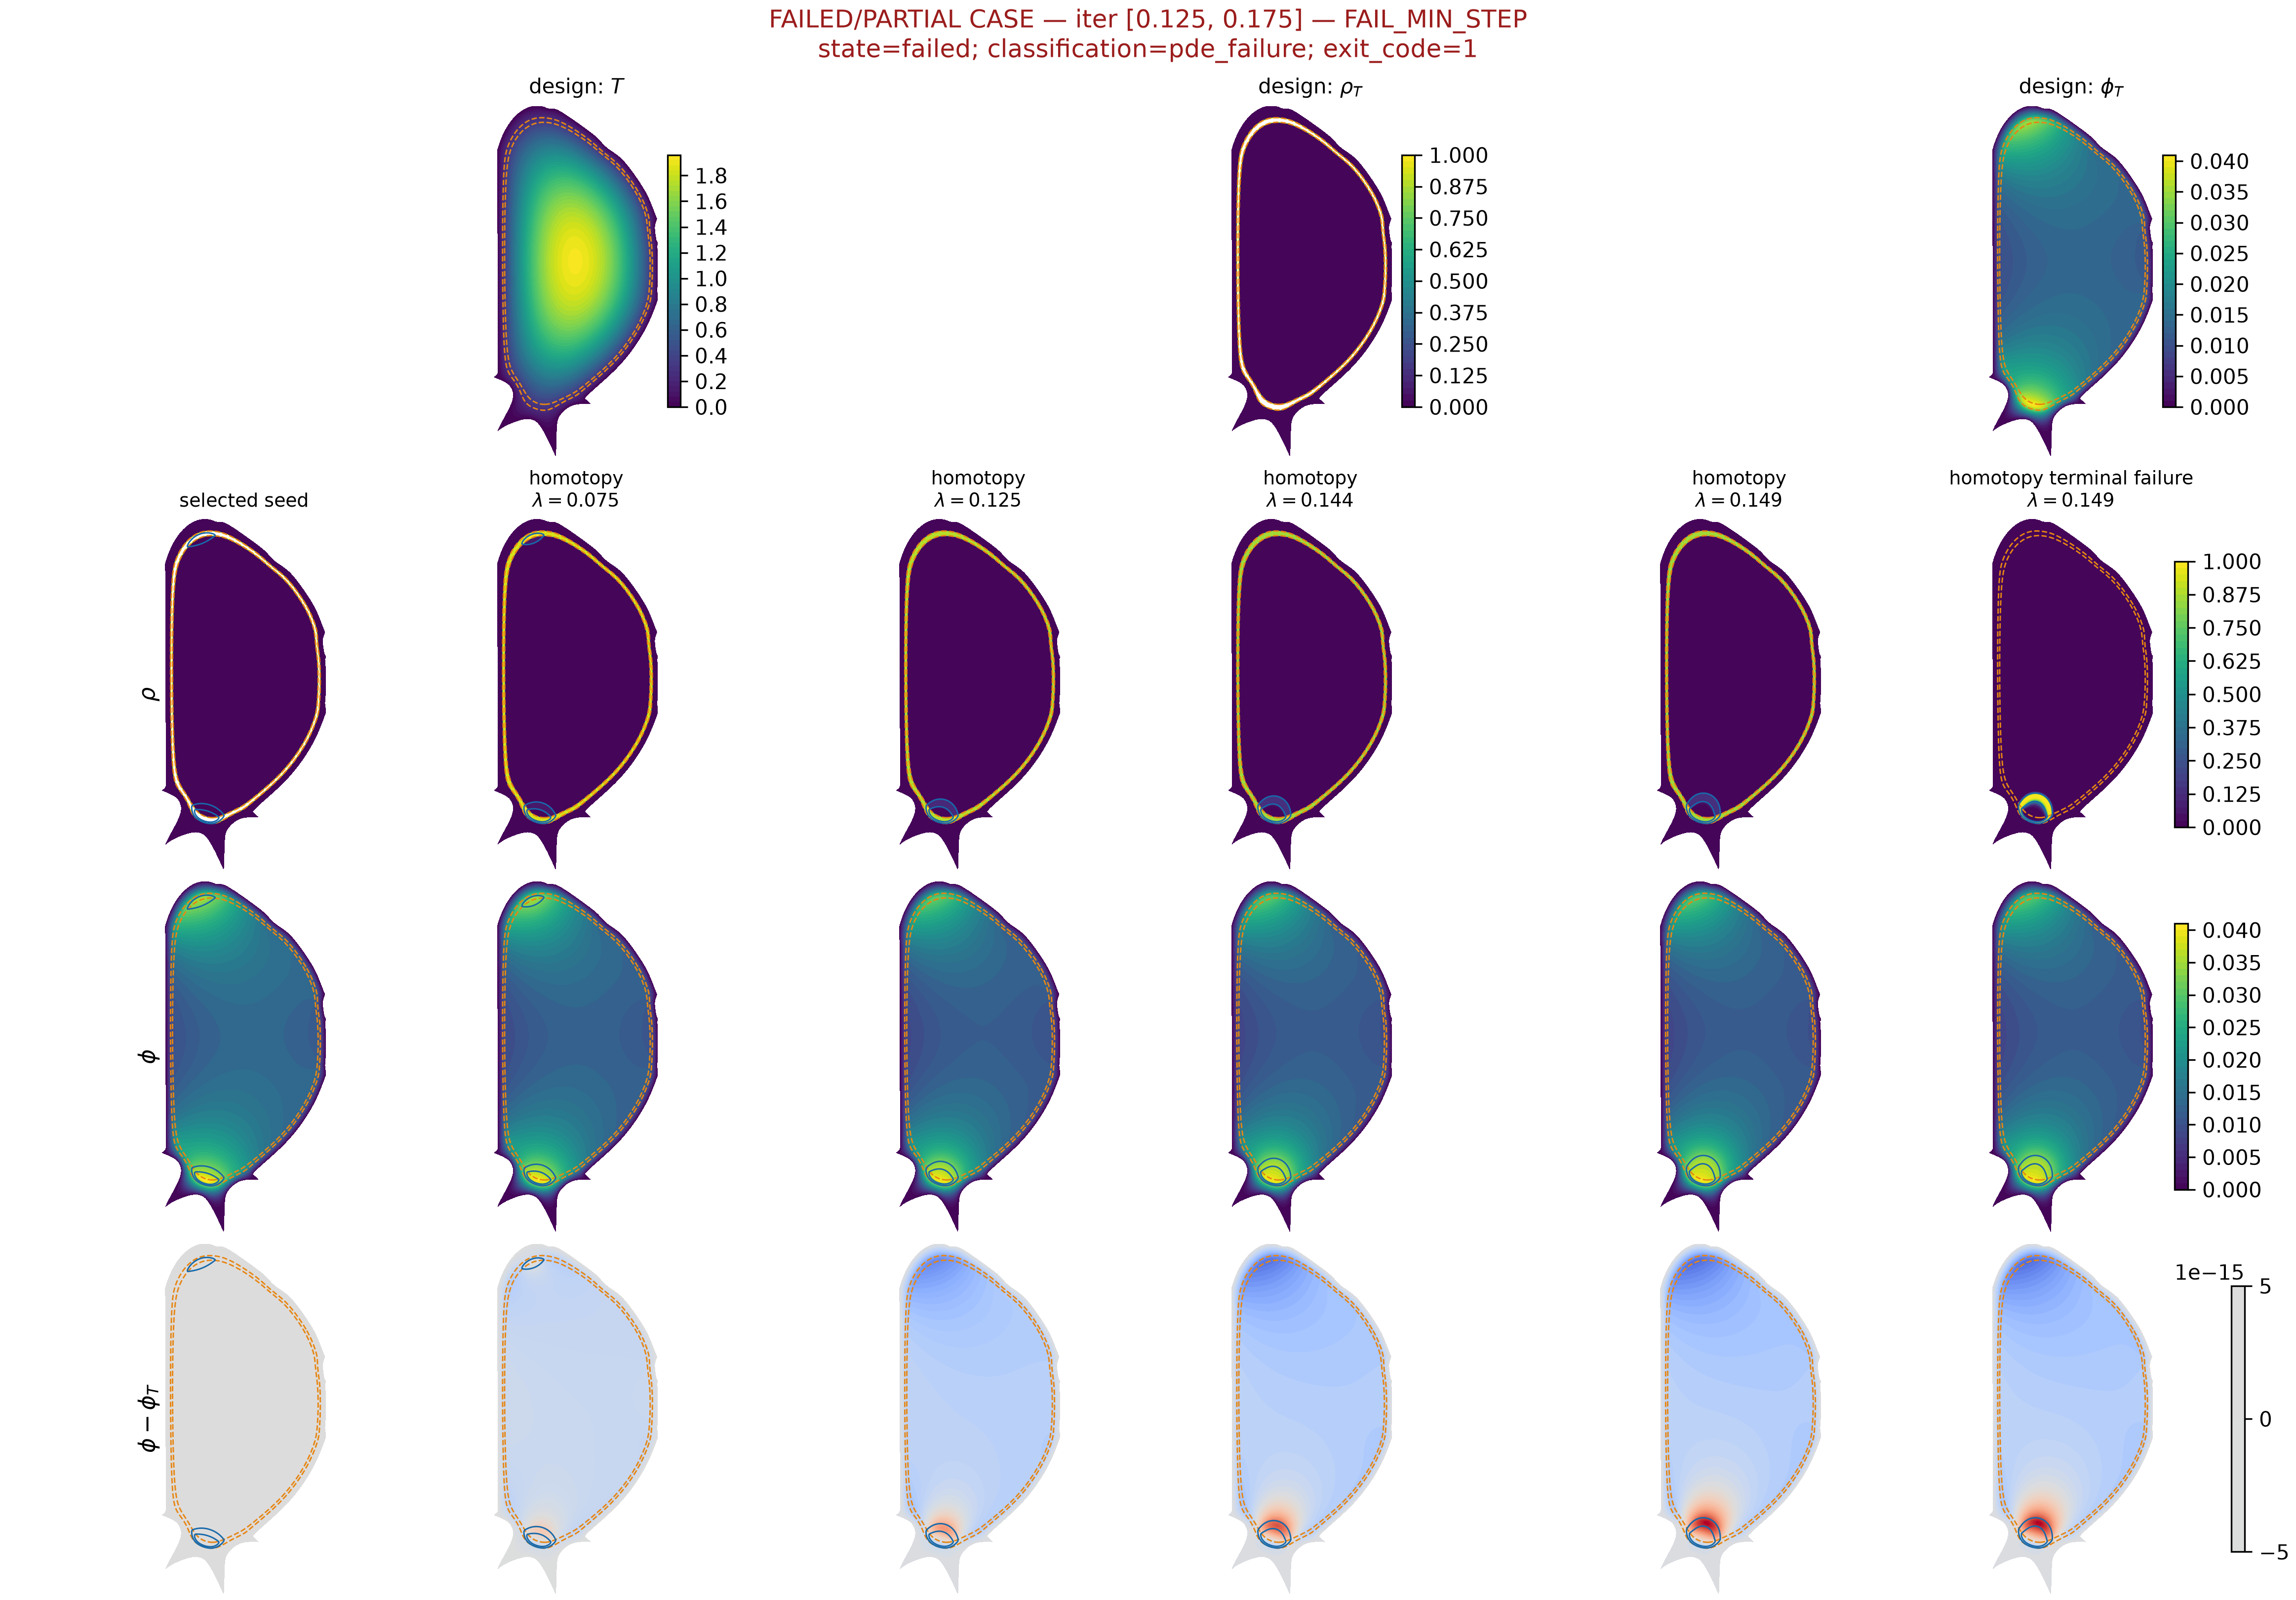
\includegraphics[width=0.88\linewidth]{figures/failed_band_evolution_048_iter_0p125_0p175_trajectory_candidate-iter-bcf30a64c685.png}
\caption{Supplemental failed/partial trajectory evidence for iter at torsion levels $[0.125,0.175]$ (case trajectory\_candidate-iter-bcf30a64c685; state=failed; classification=pde\_failure). The case is retained regardless of PDE or geometric success. Orange dashed curves are the fixed target band and blue solid curves are the moving equilibrium band; when state recovery is impossible, the PNG records the reason. Data status: actual.}
\label{fig:failed-storyboard-trajectory-candidate-iter-bcf30a64c685}
\end{figure}

\begin{figure}[tbp]
\centering
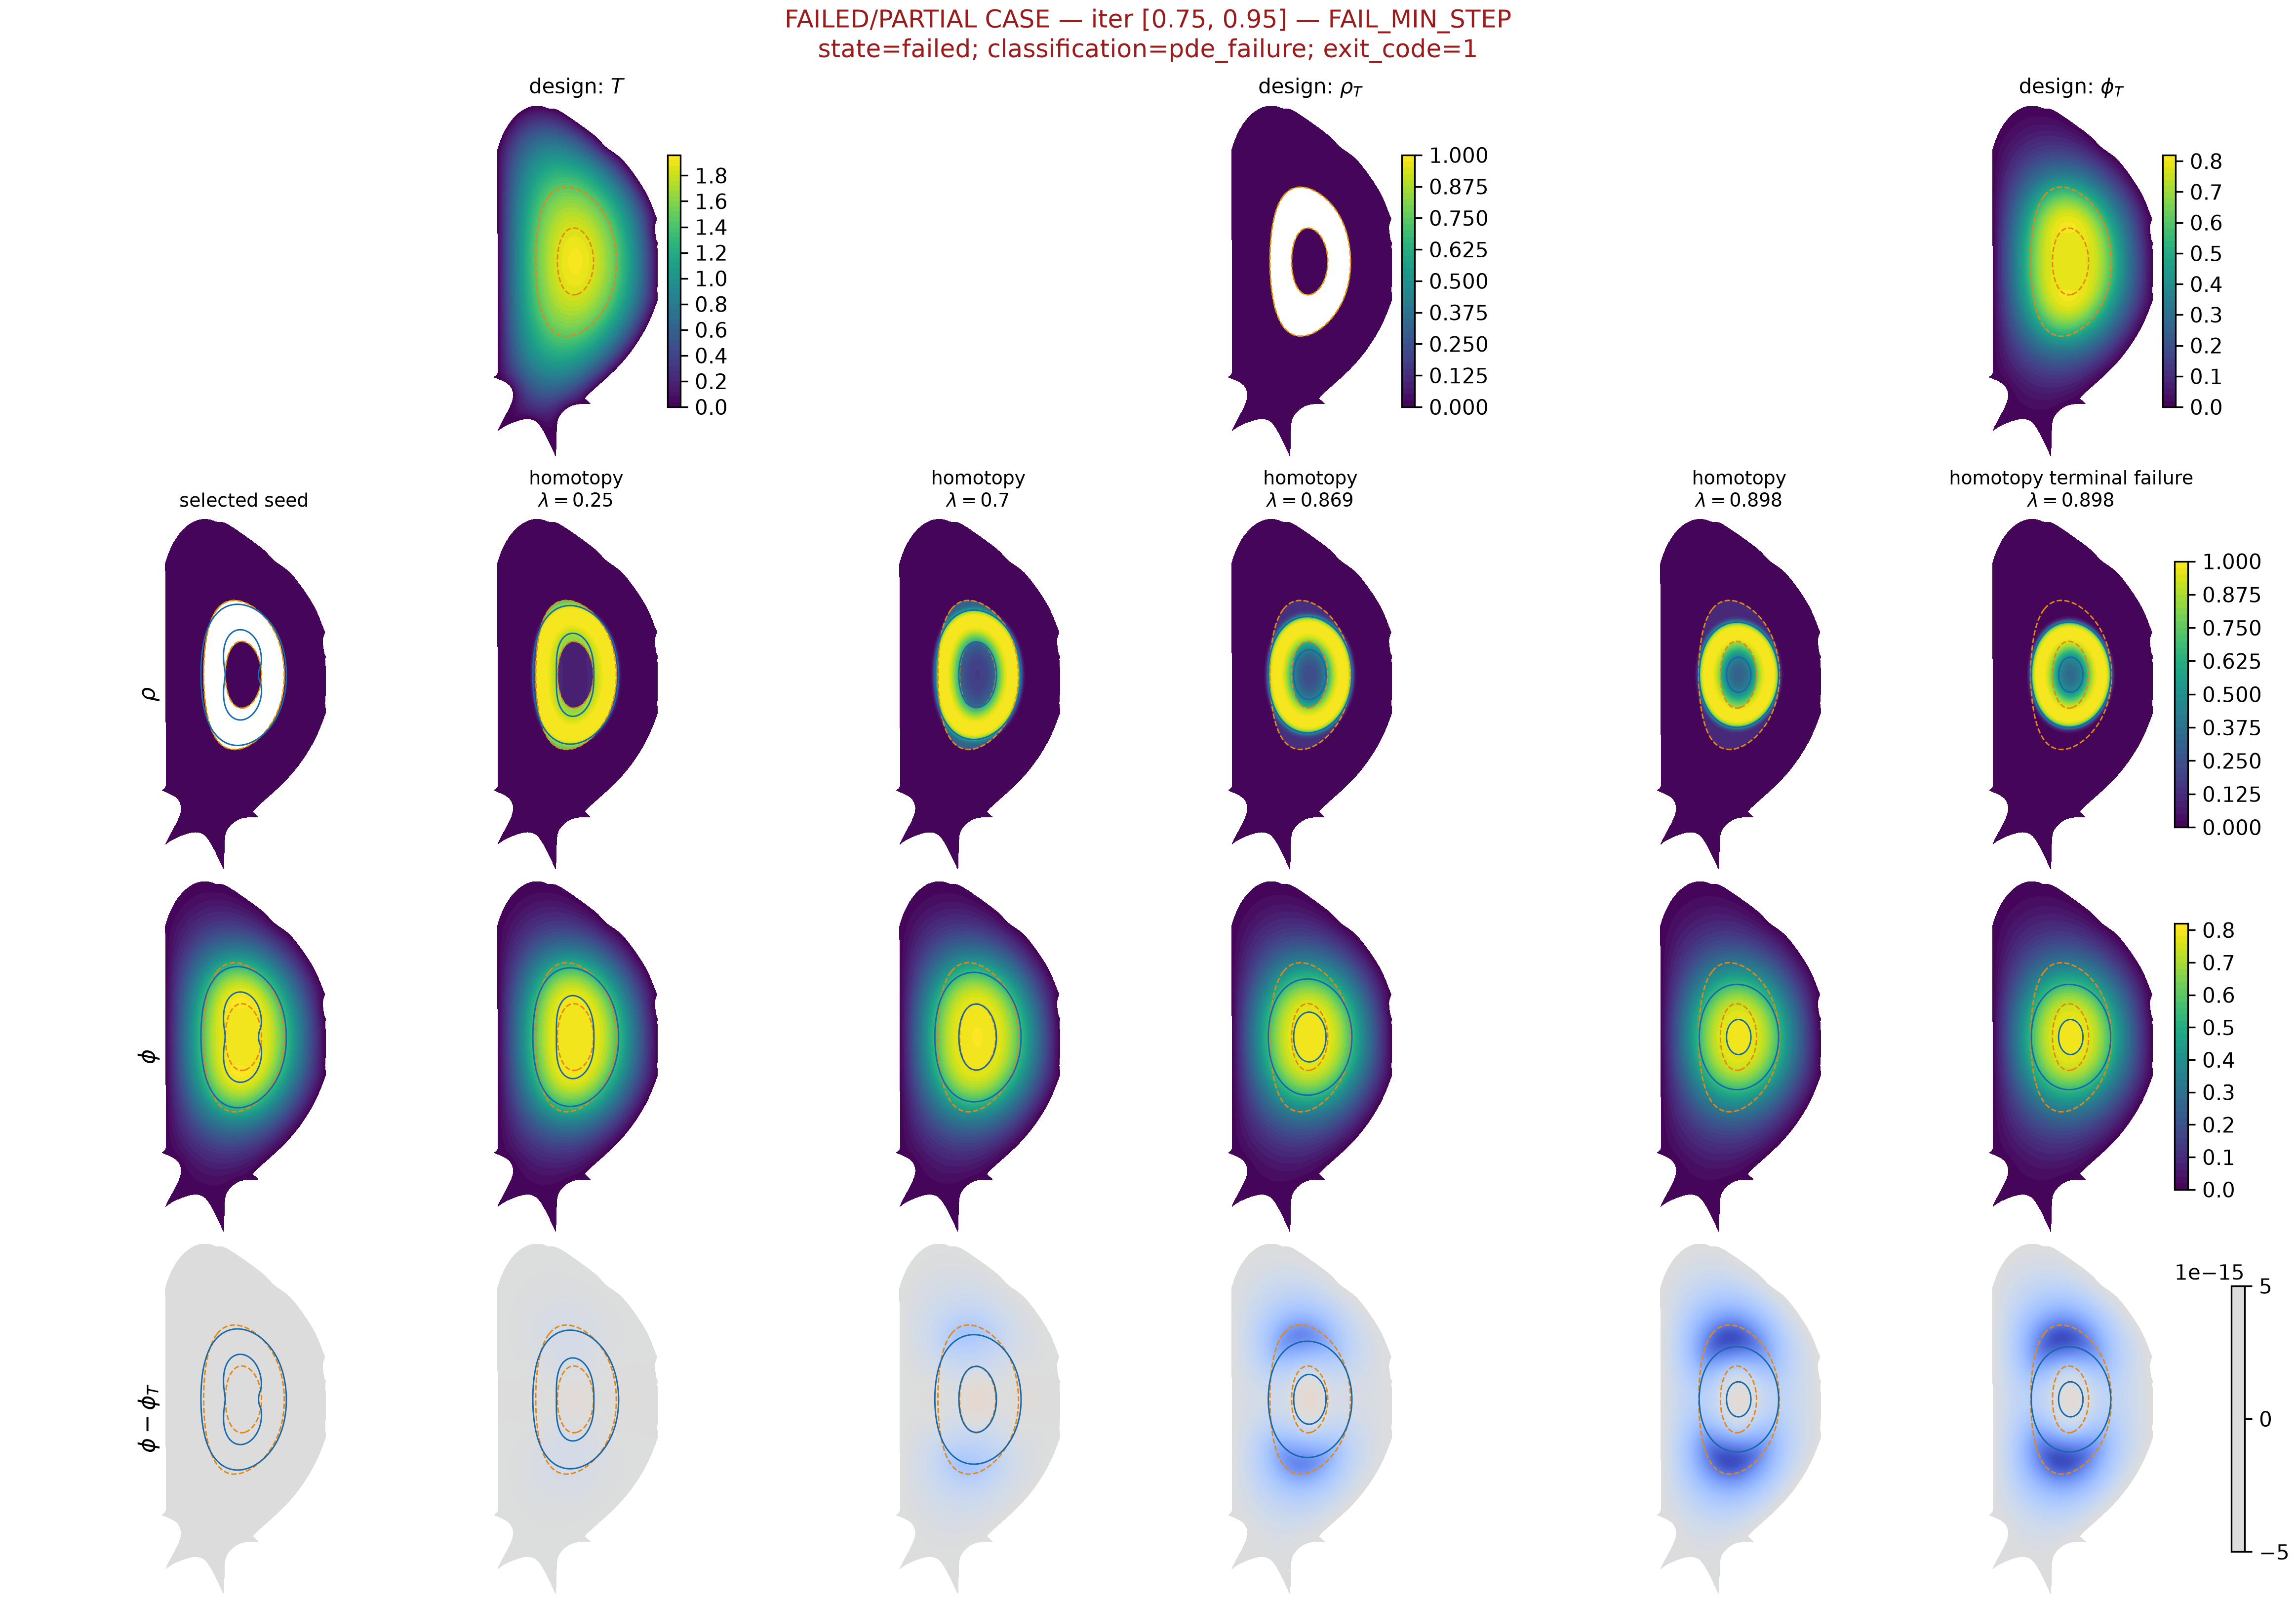
\includegraphics[width=0.88\linewidth]{figures/failed_band_evolution_049_iter_0p75_0p95_trajectory_candidate-iter-c24757c6210b.png}
\caption{Supplemental failed/partial trajectory evidence for iter at torsion levels $[0.75,0.95]$ (case trajectory\_candidate-iter-c24757c6210b; state=failed; classification=pde\_failure). The case is retained regardless of PDE or geometric success. Orange dashed curves are the fixed target band and blue solid curves are the moving equilibrium band; when state recovery is impossible, the PNG records the reason. Data status: actual.}
\label{fig:failed-storyboard-trajectory-candidate-iter-c24757c6210b}
\end{figure}

\begin{figure}[tbp]
\centering
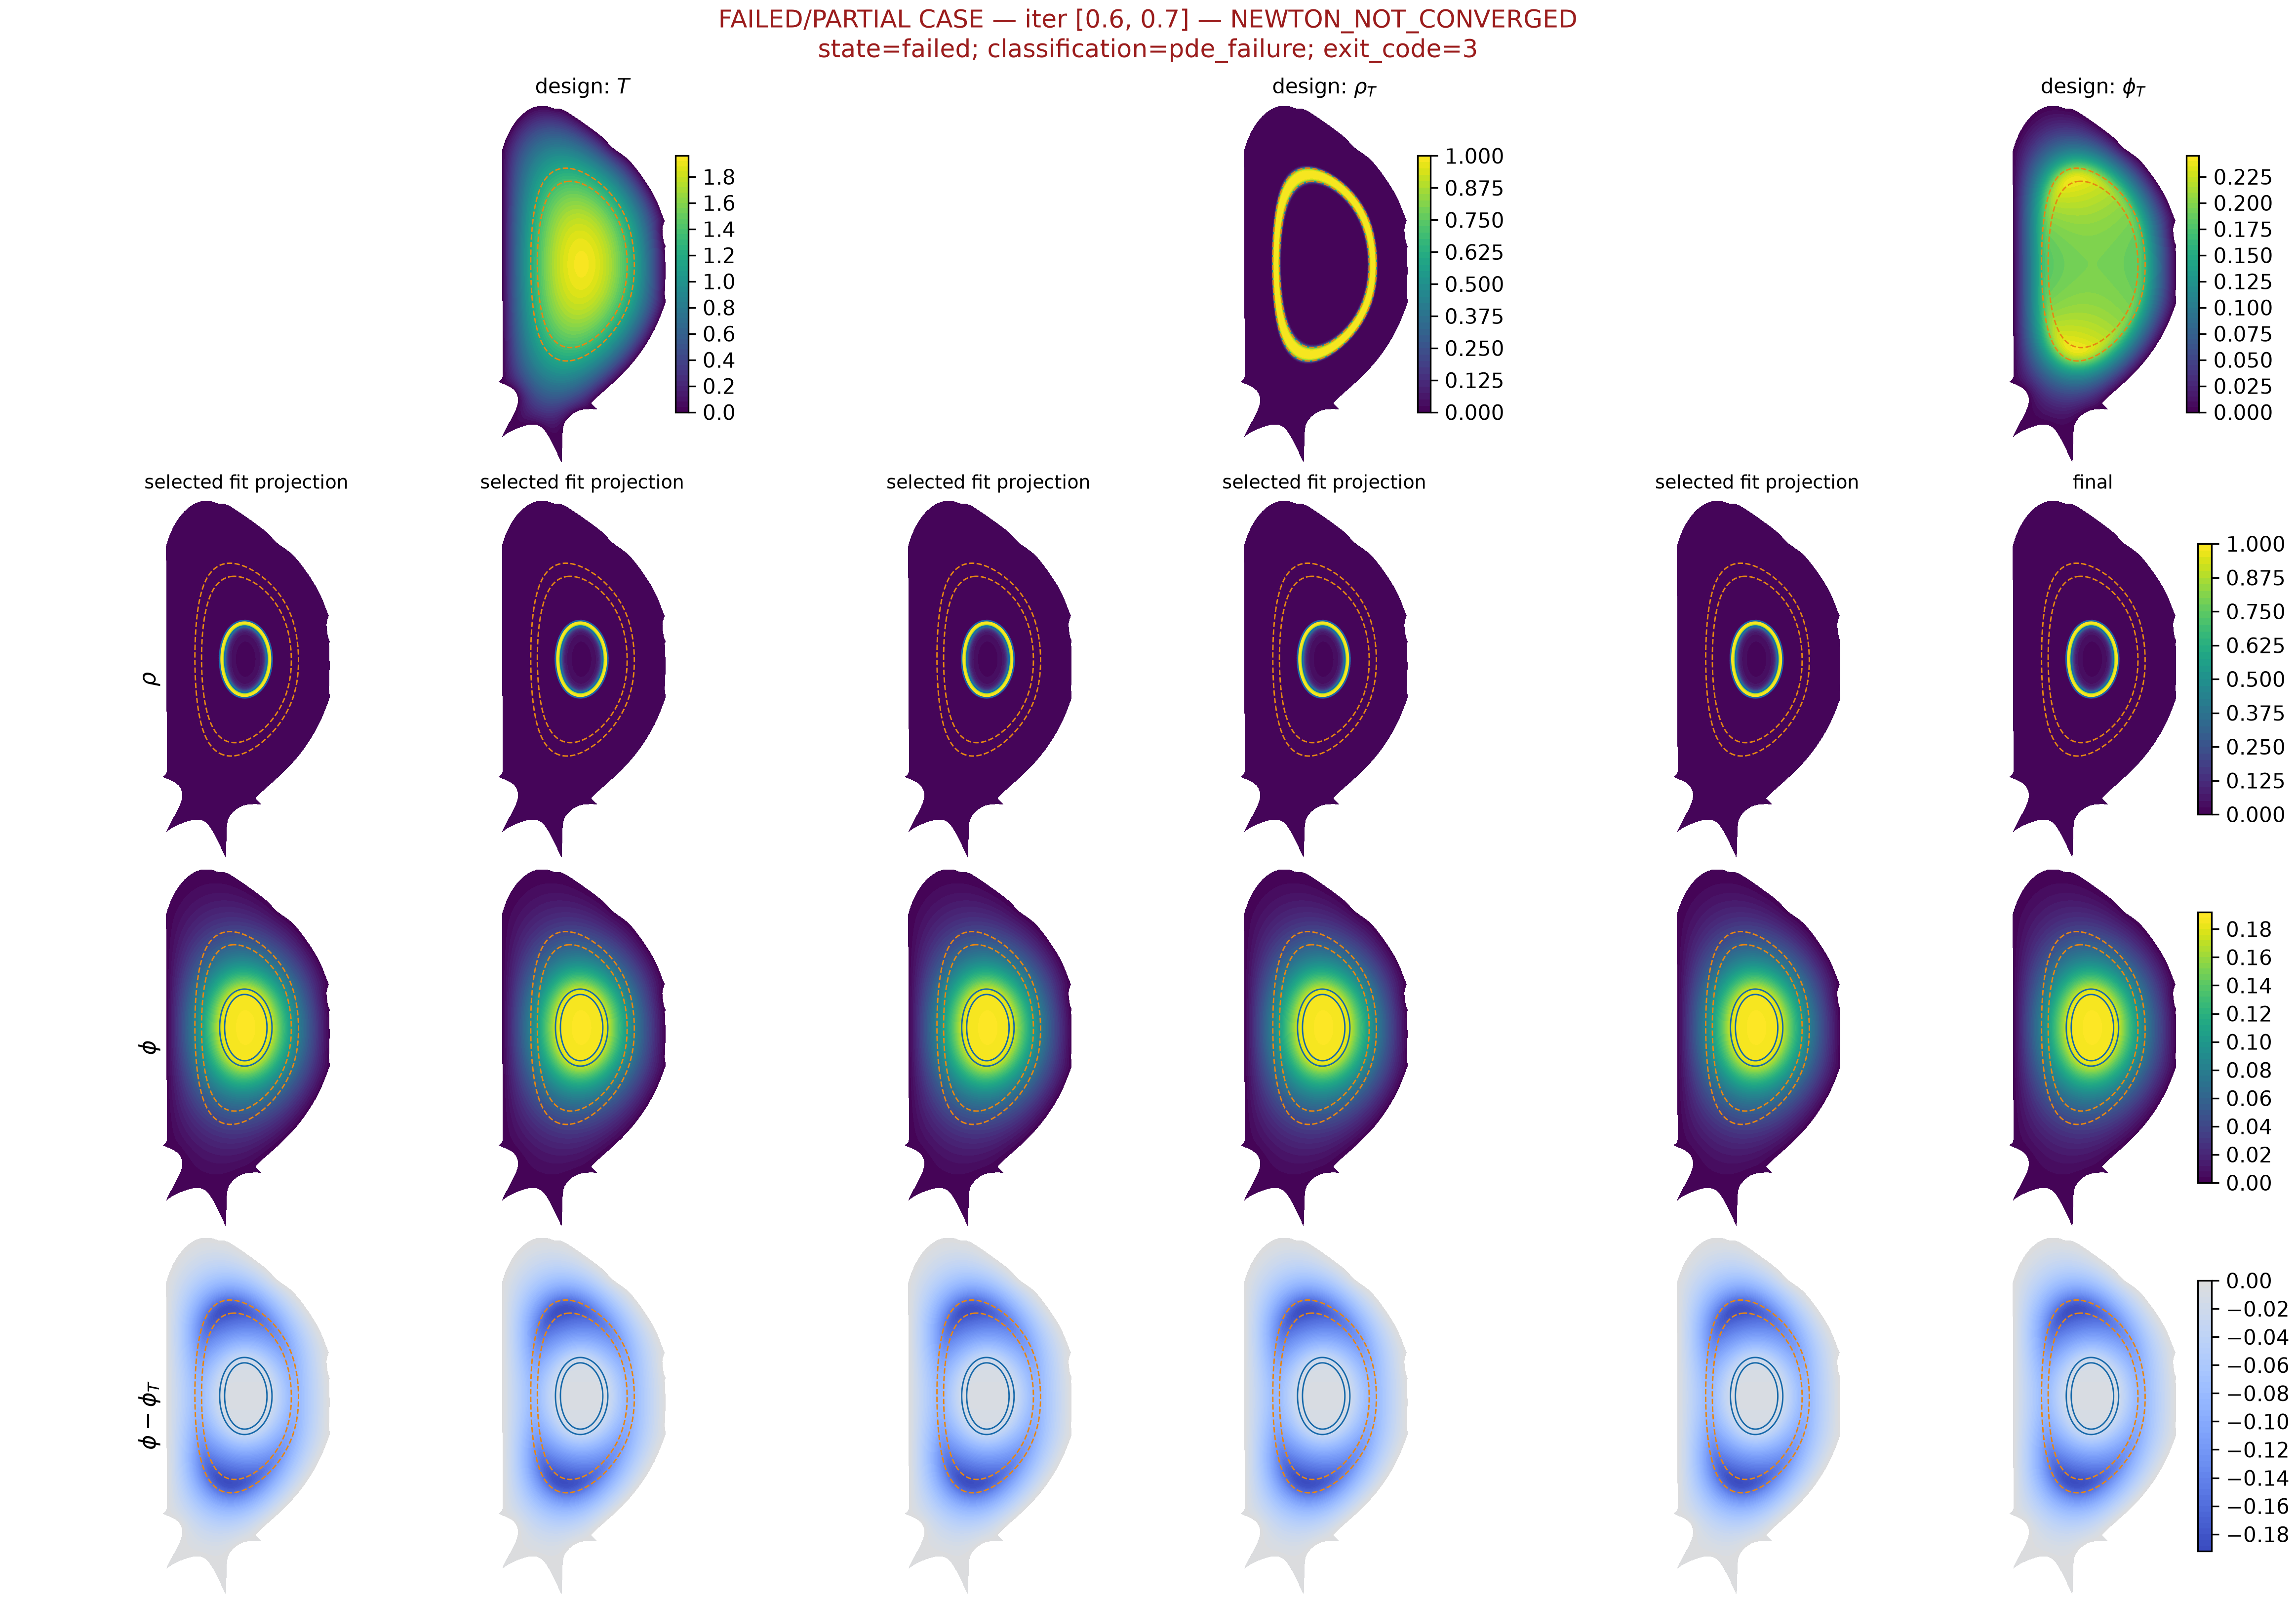
\includegraphics[width=0.88\linewidth]{figures/failed_band_evolution_050_iter_0p6_0p7_trajectory_fit_rescue-iter-12c57975d4d5.png}
\caption{Supplemental failed/partial trajectory evidence for iter at torsion levels $[0.6,0.7]$ (case trajectory\_fit\_rescue-iter-12c57975d4d5; state=failed; classification=pde\_failure). The case is retained regardless of PDE or geometric success. Orange dashed curves are the fixed target band and blue solid curves are the moving equilibrium band; when state recovery is impossible, the PNG records the reason. Data status: actual.}
\label{fig:failed-storyboard-trajectory-fit-rescue-iter-12c57975d4d5}
\end{figure}

\begin{figure}[tbp]
\centering
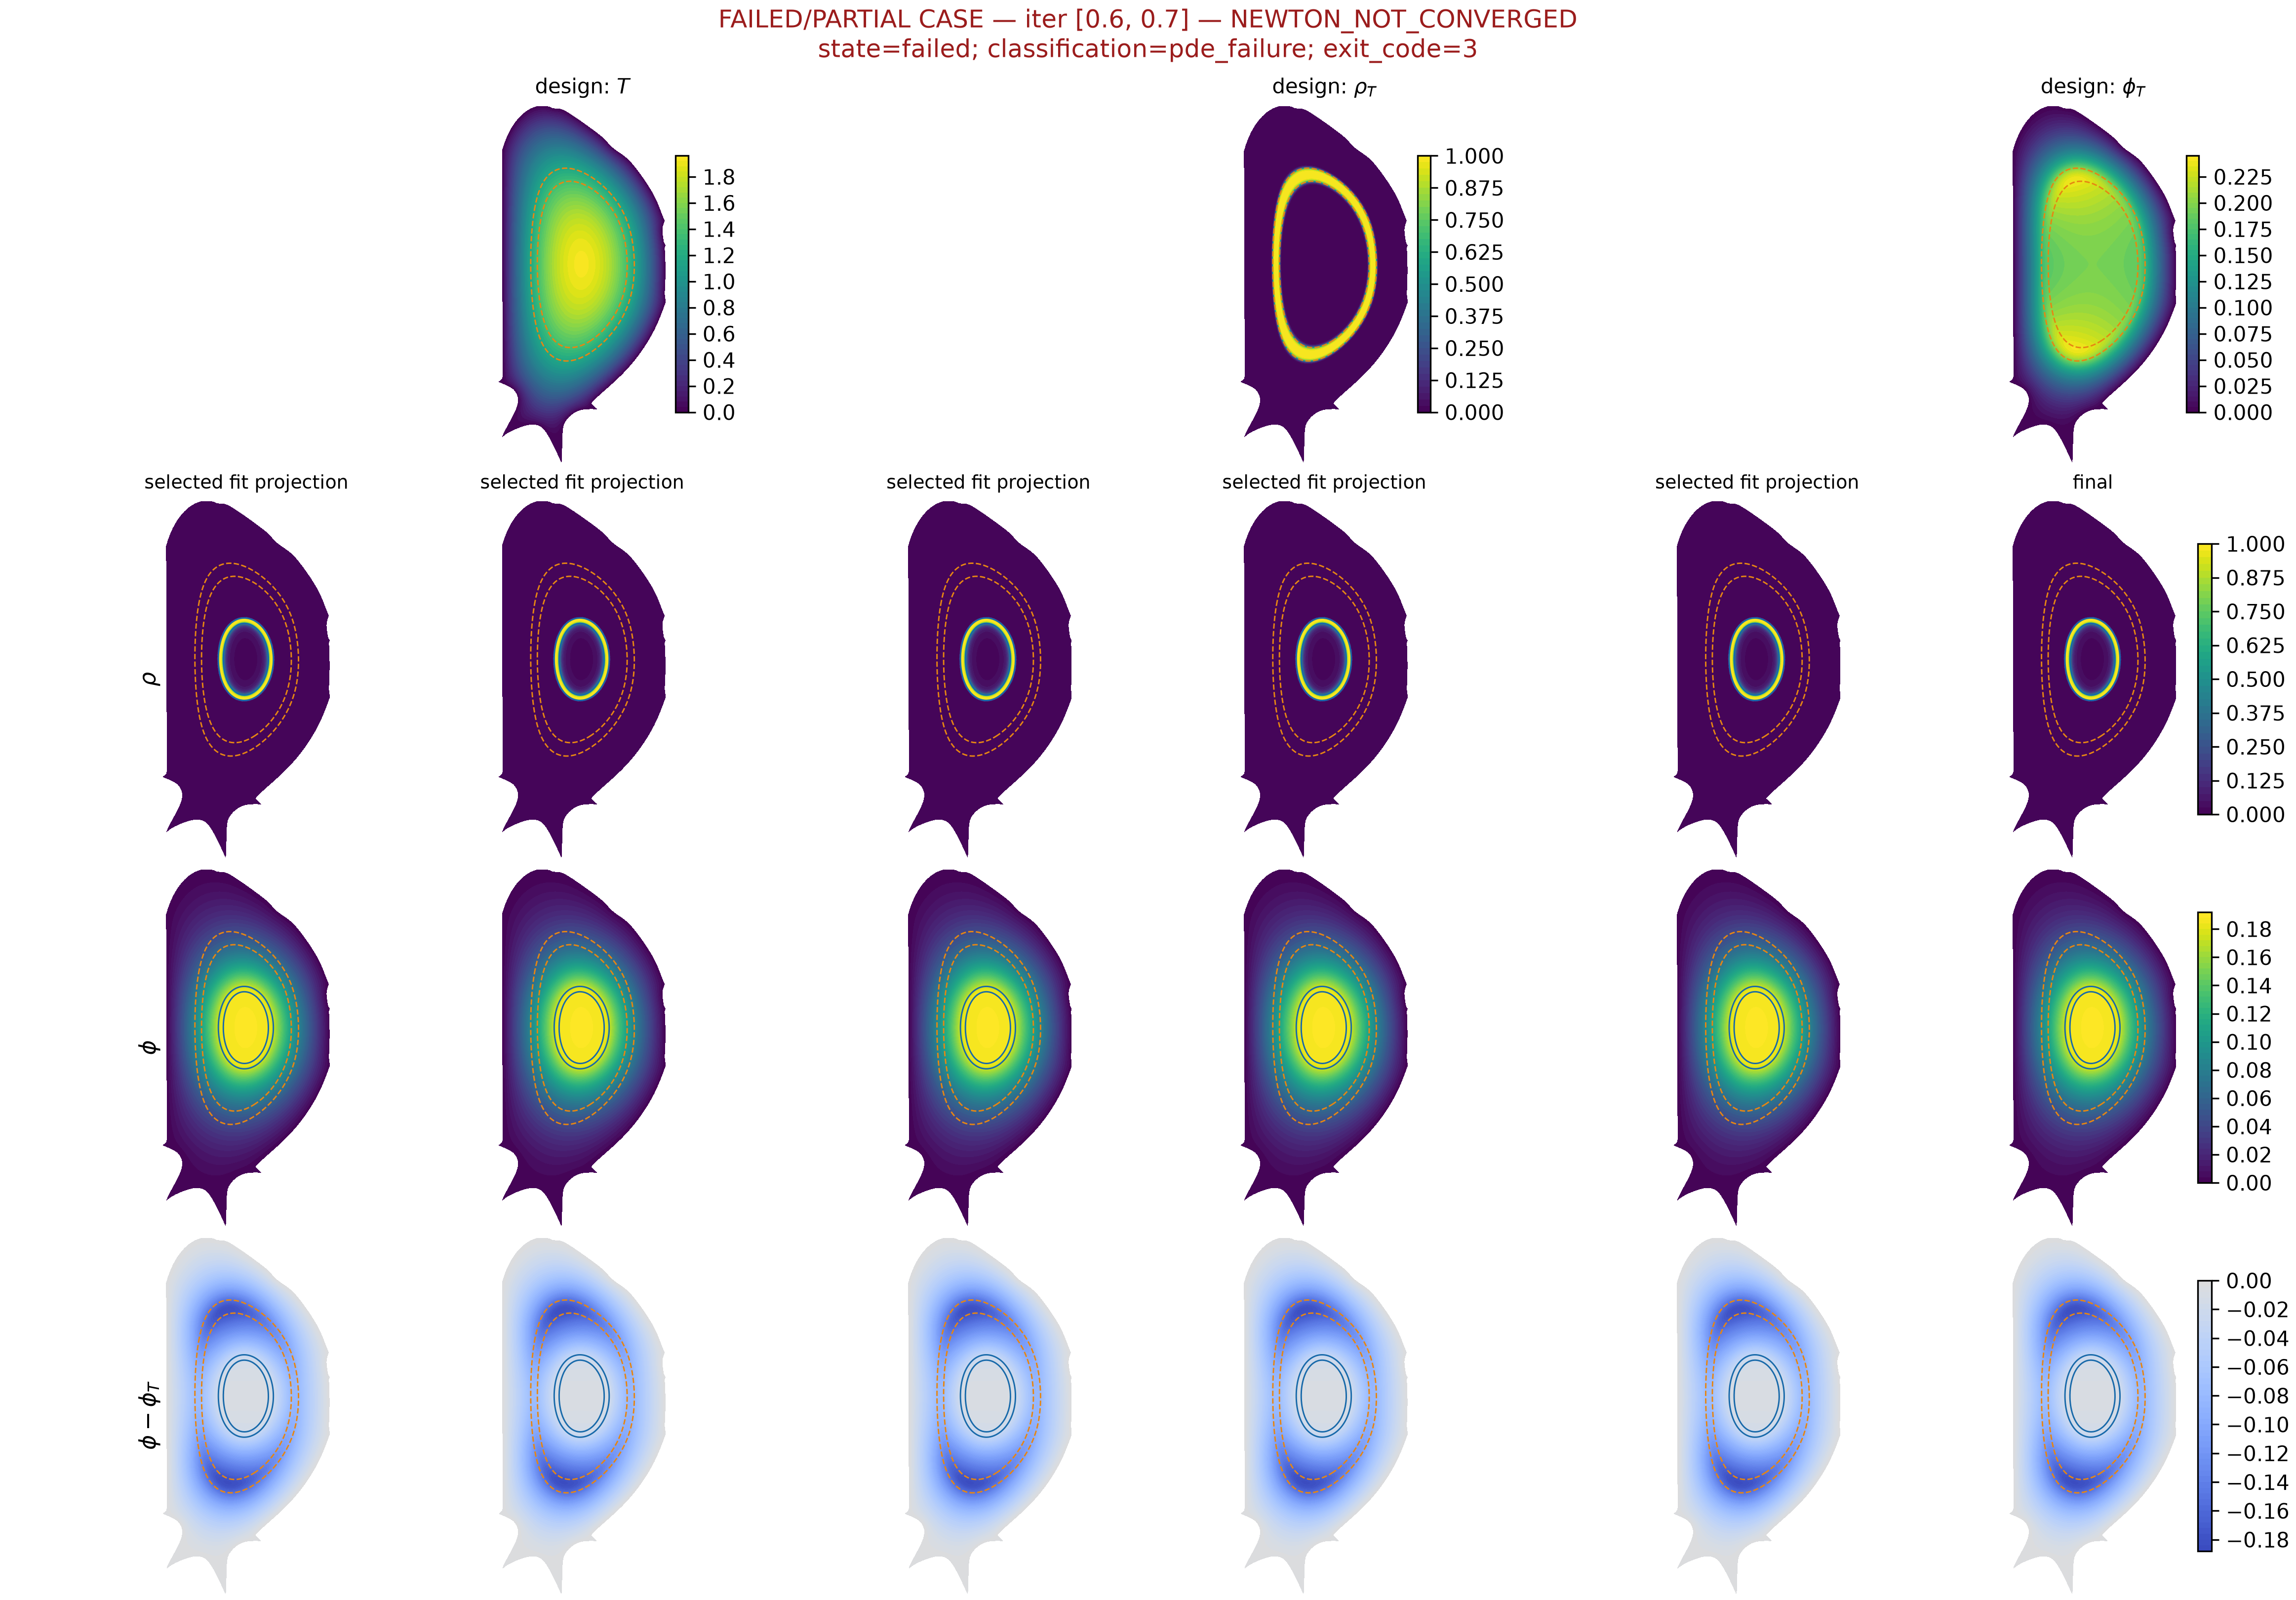
\includegraphics[width=0.88\linewidth]{figures/failed_band_evolution_051_iter_0p6_0p7_trajectory_iter_window_fit_high_newton_v3-iter-8997eebadb46.png}
\caption{Supplemental failed/partial trajectory evidence for iter at torsion levels $[0.6,0.7]$ (case trajectory\_iter\_window\_fit\_high\_newton\_v3-iter-8997eebadb46; state=failed; classification=pde\_failure). The case is retained regardless of PDE or geometric success. Orange dashed curves are the fixed target band and blue solid curves are the moving equilibrium band; when state recovery is impossible, the PNG records the reason. Data status: actual.}
\label{fig:failed-storyboard-trajectory-iter-window-fit-high-newton-v3-iter-8997eebadb46}
\end{figure}

\begin{figure}[tbp]
\centering
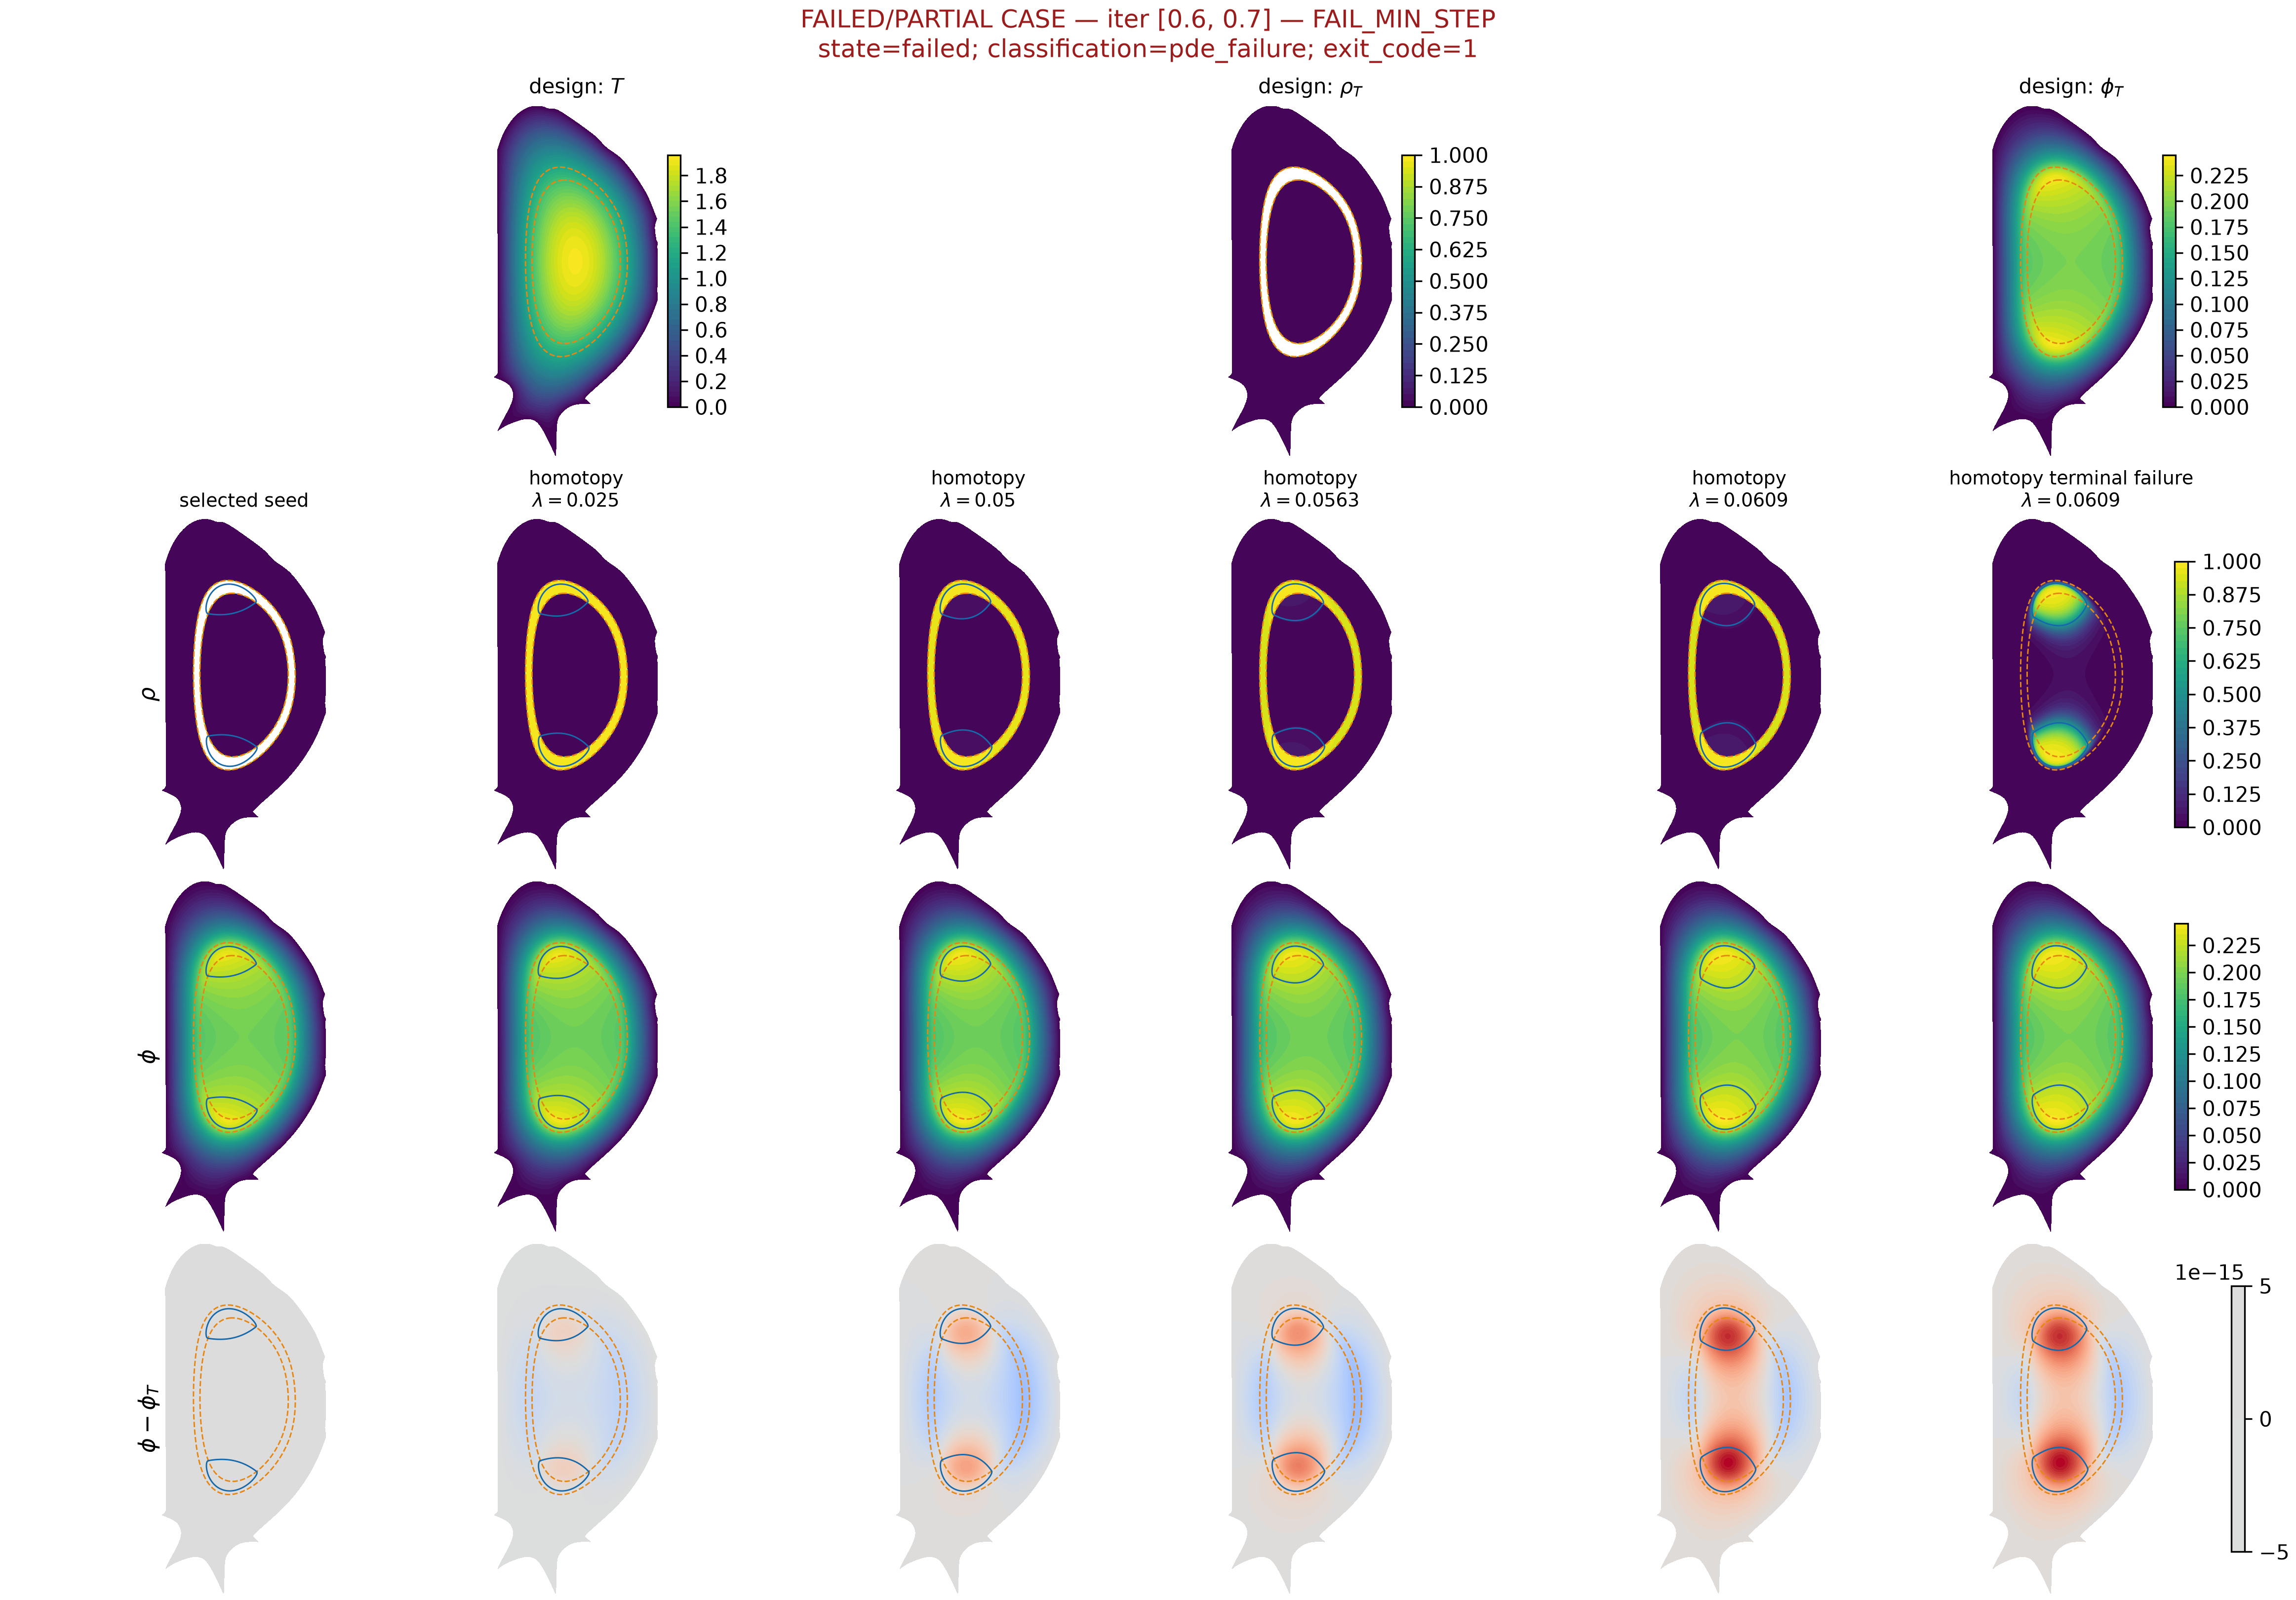
\includegraphics[width=0.88\linewidth]{figures/failed_band_evolution_052_iter_0p6_0p7_trajectory_rescue-iter-298b59ece73a.png}
\caption{Supplemental failed/partial trajectory evidence for iter at torsion levels $[0.6,0.7]$ (case trajectory\_rescue-iter-298b59ece73a; state=failed; classification=pde\_failure). The case is retained regardless of PDE or geometric success. Orange dashed curves are the fixed target band and blue solid curves are the moving equilibrium band; when state recovery is impossible, the PNG records the reason. Data status: actual.}
\label{fig:failed-storyboard-trajectory-rescue-iter-298b59ece73a}
\end{figure}

\begin{figure}[tbp]
\centering
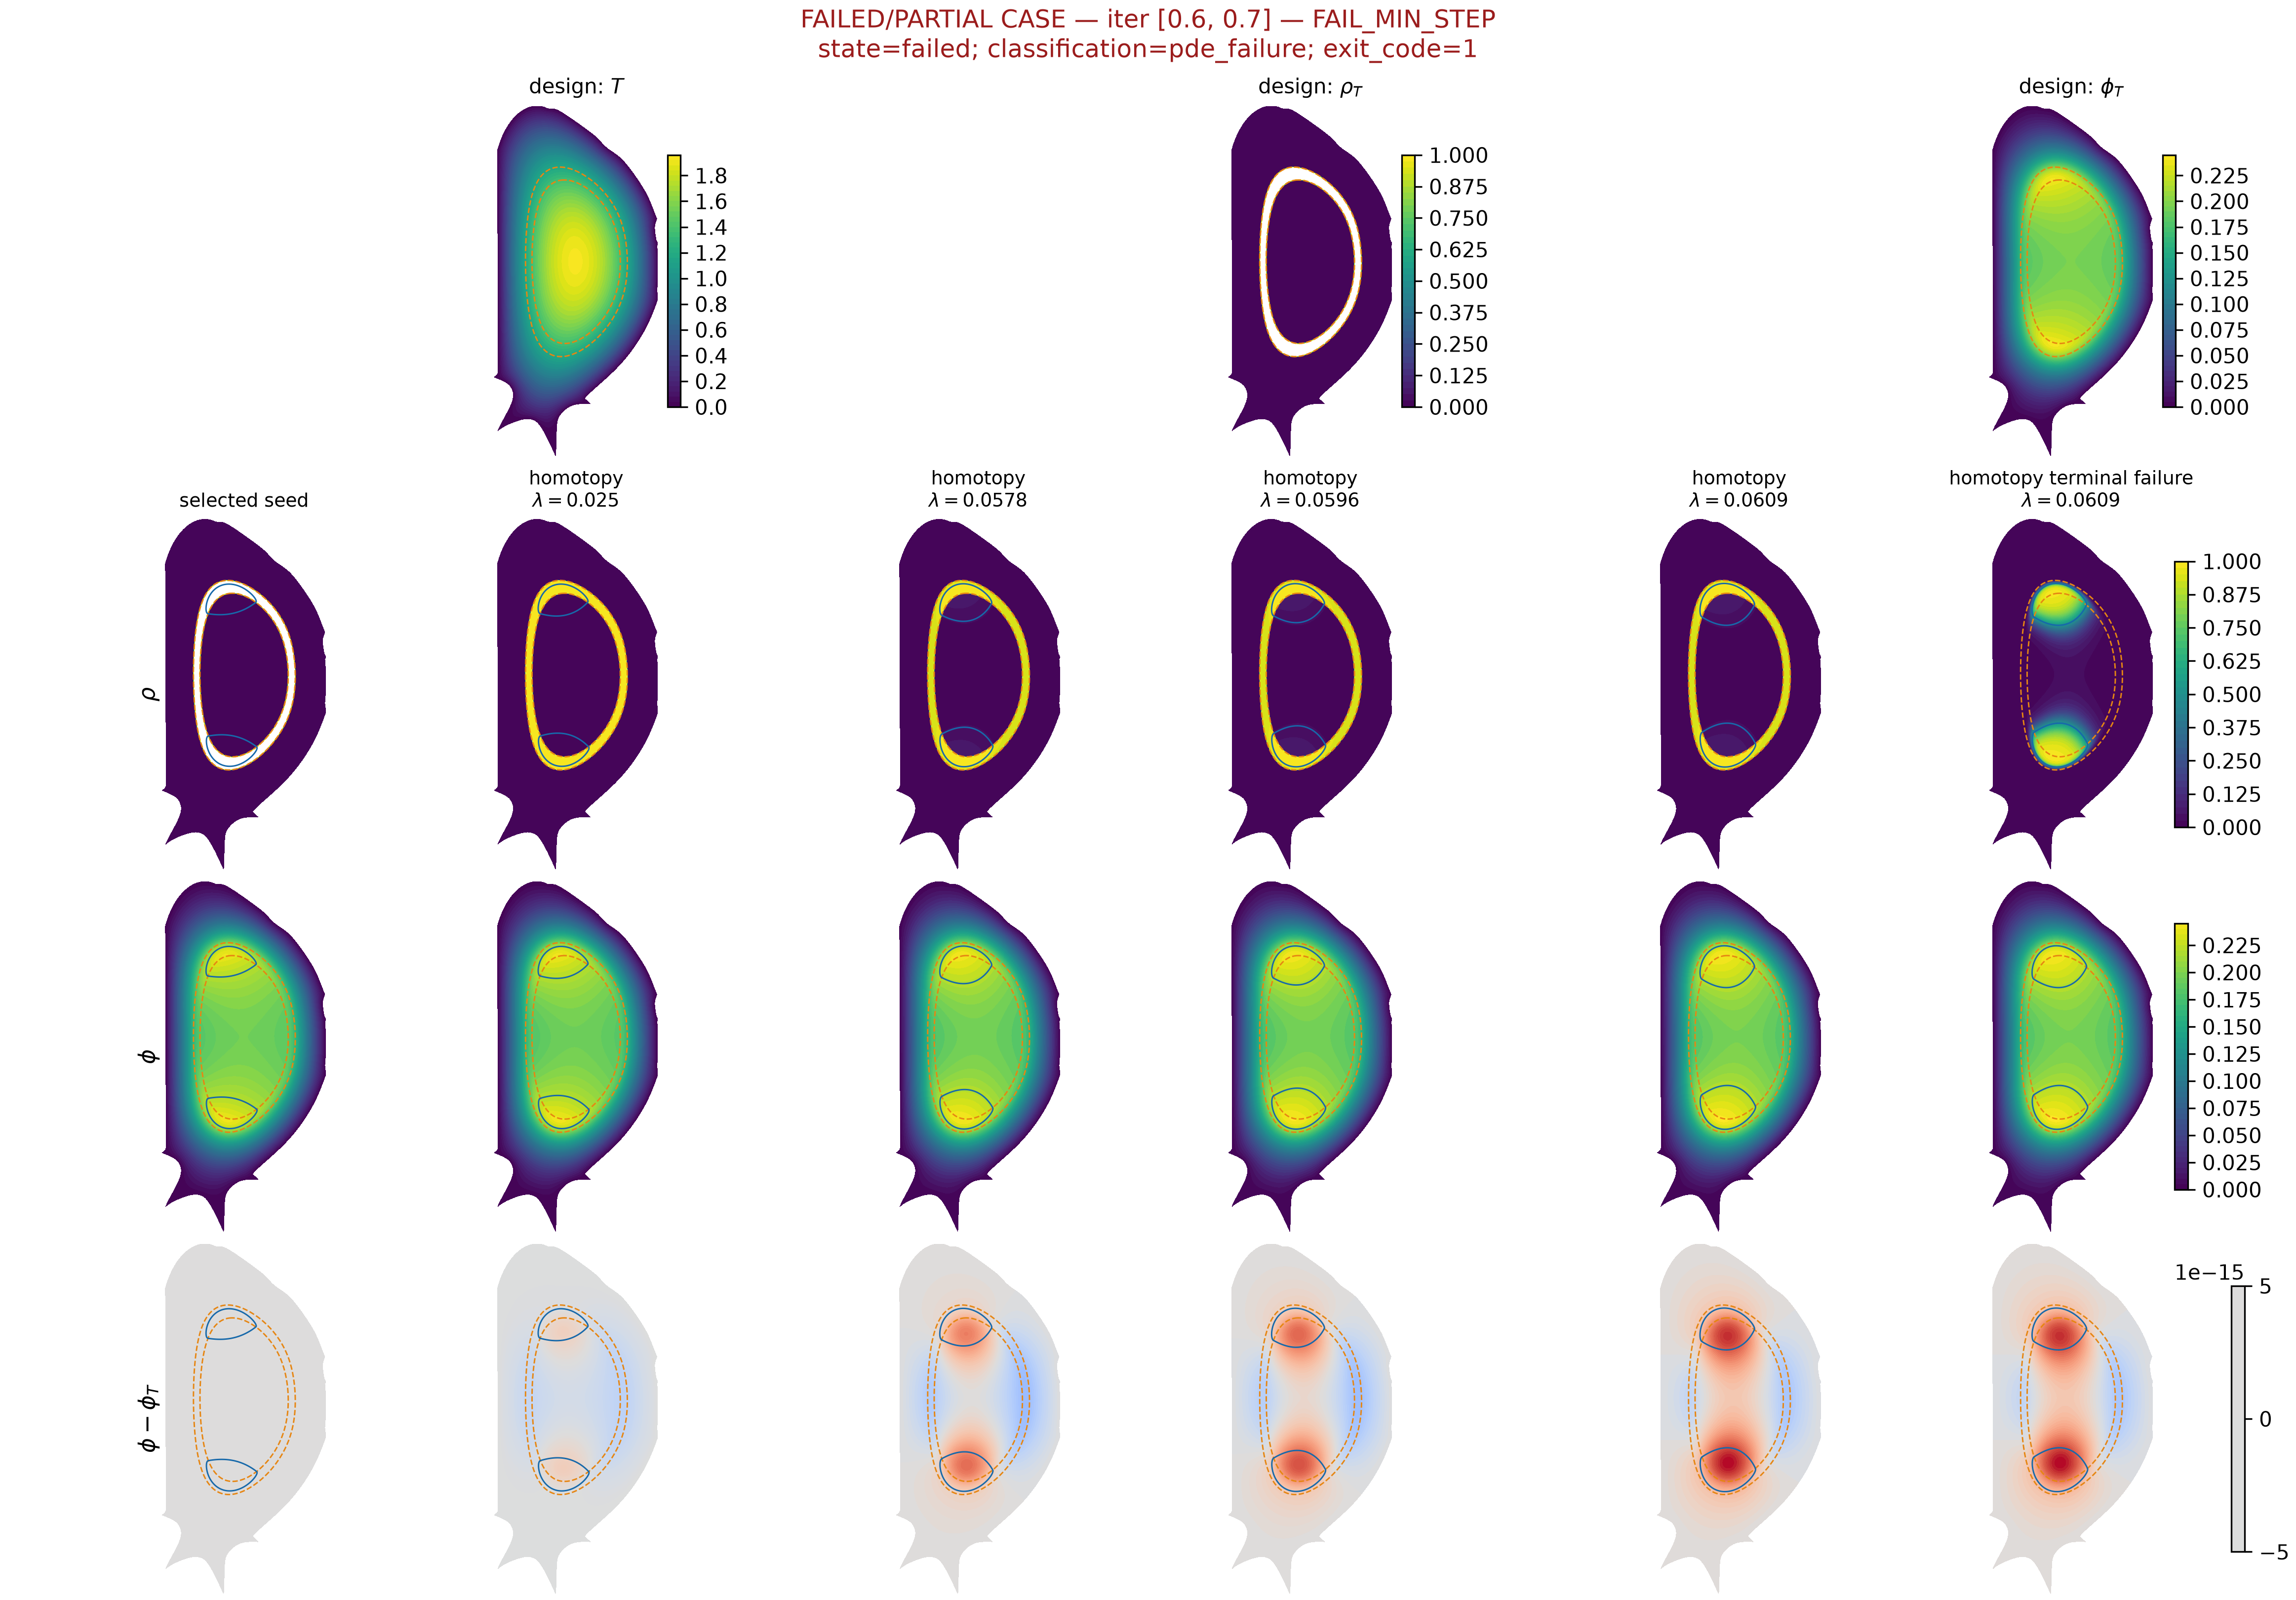
\includegraphics[width=0.88\linewidth]{figures/failed_band_evolution_053_iter_0p6_0p7_trajectory_rescue-iter-cee449f0dc48.png}
\caption{Supplemental failed/partial trajectory evidence for iter at torsion levels $[0.6,0.7]$ (case trajectory\_rescue-iter-cee449f0dc48; state=failed; classification=pde\_failure). The case is retained regardless of PDE or geometric success. Orange dashed curves are the fixed target band and blue solid curves are the moving equilibrium band; when state recovery is impossible, the PNG records the reason. Data status: actual.}
\label{fig:failed-storyboard-trajectory-rescue-iter-cee449f0dc48}
\end{figure}

\clearpage

\begin{figure}[tbp]
\centering
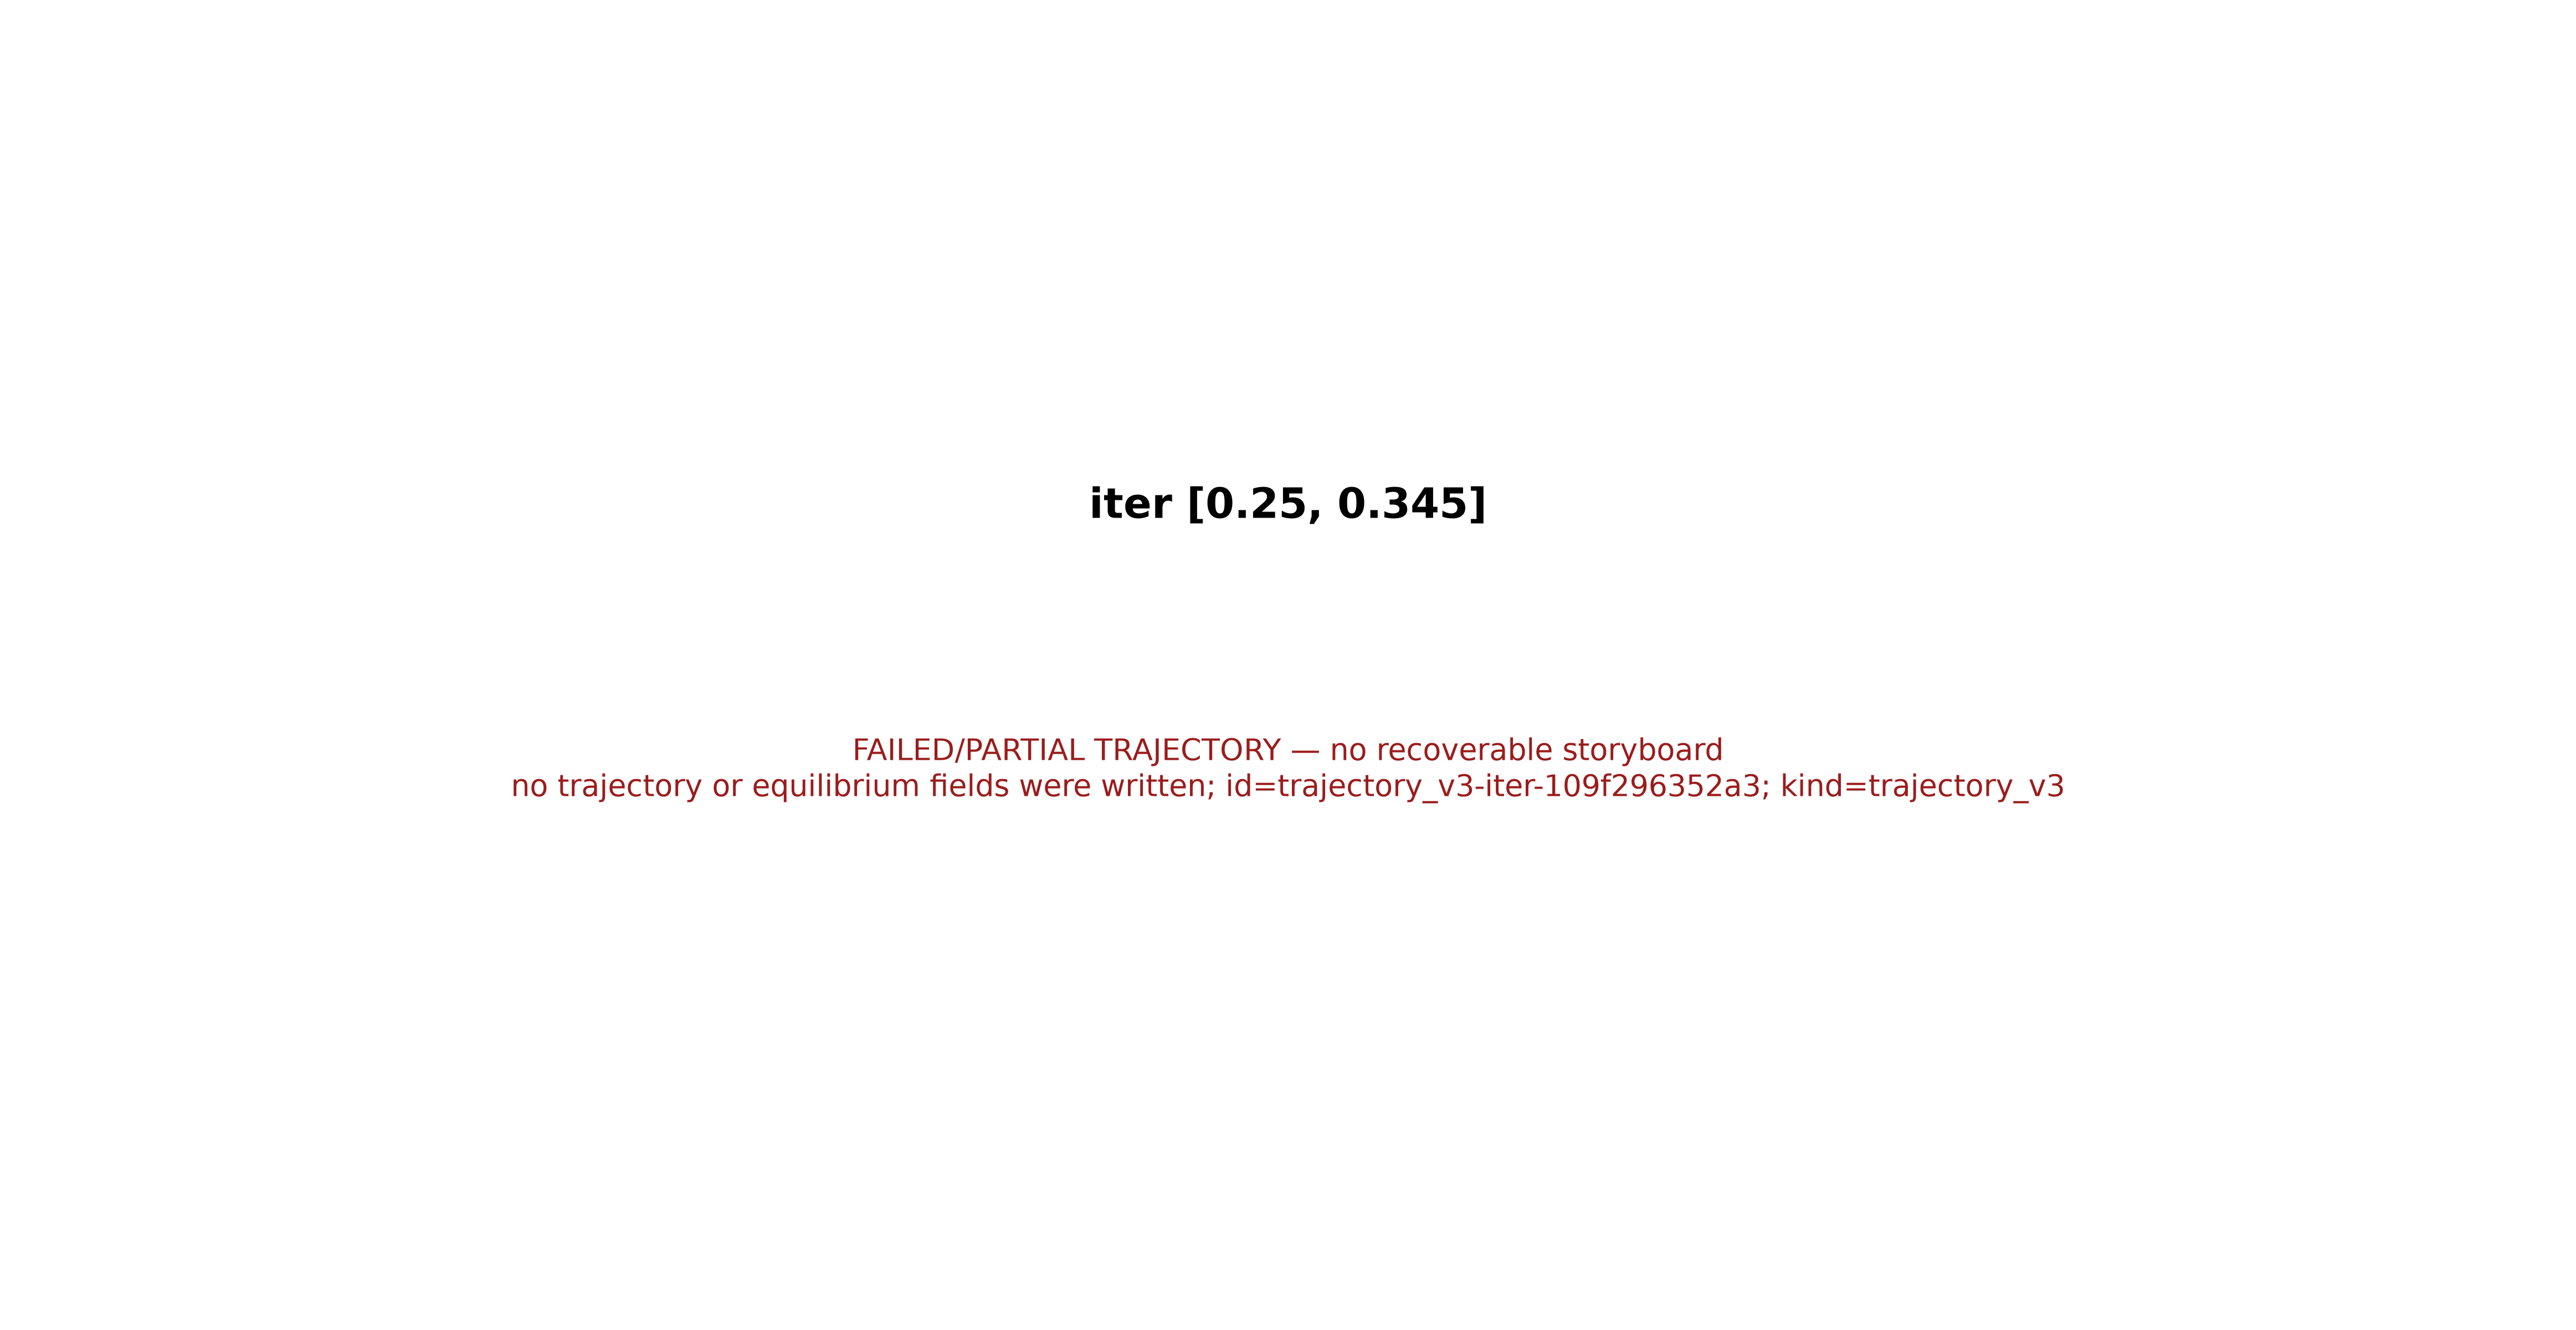
\includegraphics[width=0.88\linewidth]{figures/failed_band_evolution_054_iter_0p25_0p345_trajectory_v3-iter-109f296352a3.png}
\caption{Supplemental failed/partial trajectory evidence for iter at torsion levels $[0.25,0.345]$ (case trajectory\_v3-iter-109f296352a3; state=deferred; classification=deferred). The case is retained regardless of PDE or geometric success. Orange dashed curves are the fixed target band and blue solid curves are the moving equilibrium band; when state recovery is impossible, the PNG records the reason. Data status: diagnostic\_only.}
\label{fig:failed-storyboard-trajectory-v3-iter-109f296352a3}
\end{figure}

\begin{figure}[tbp]
\centering
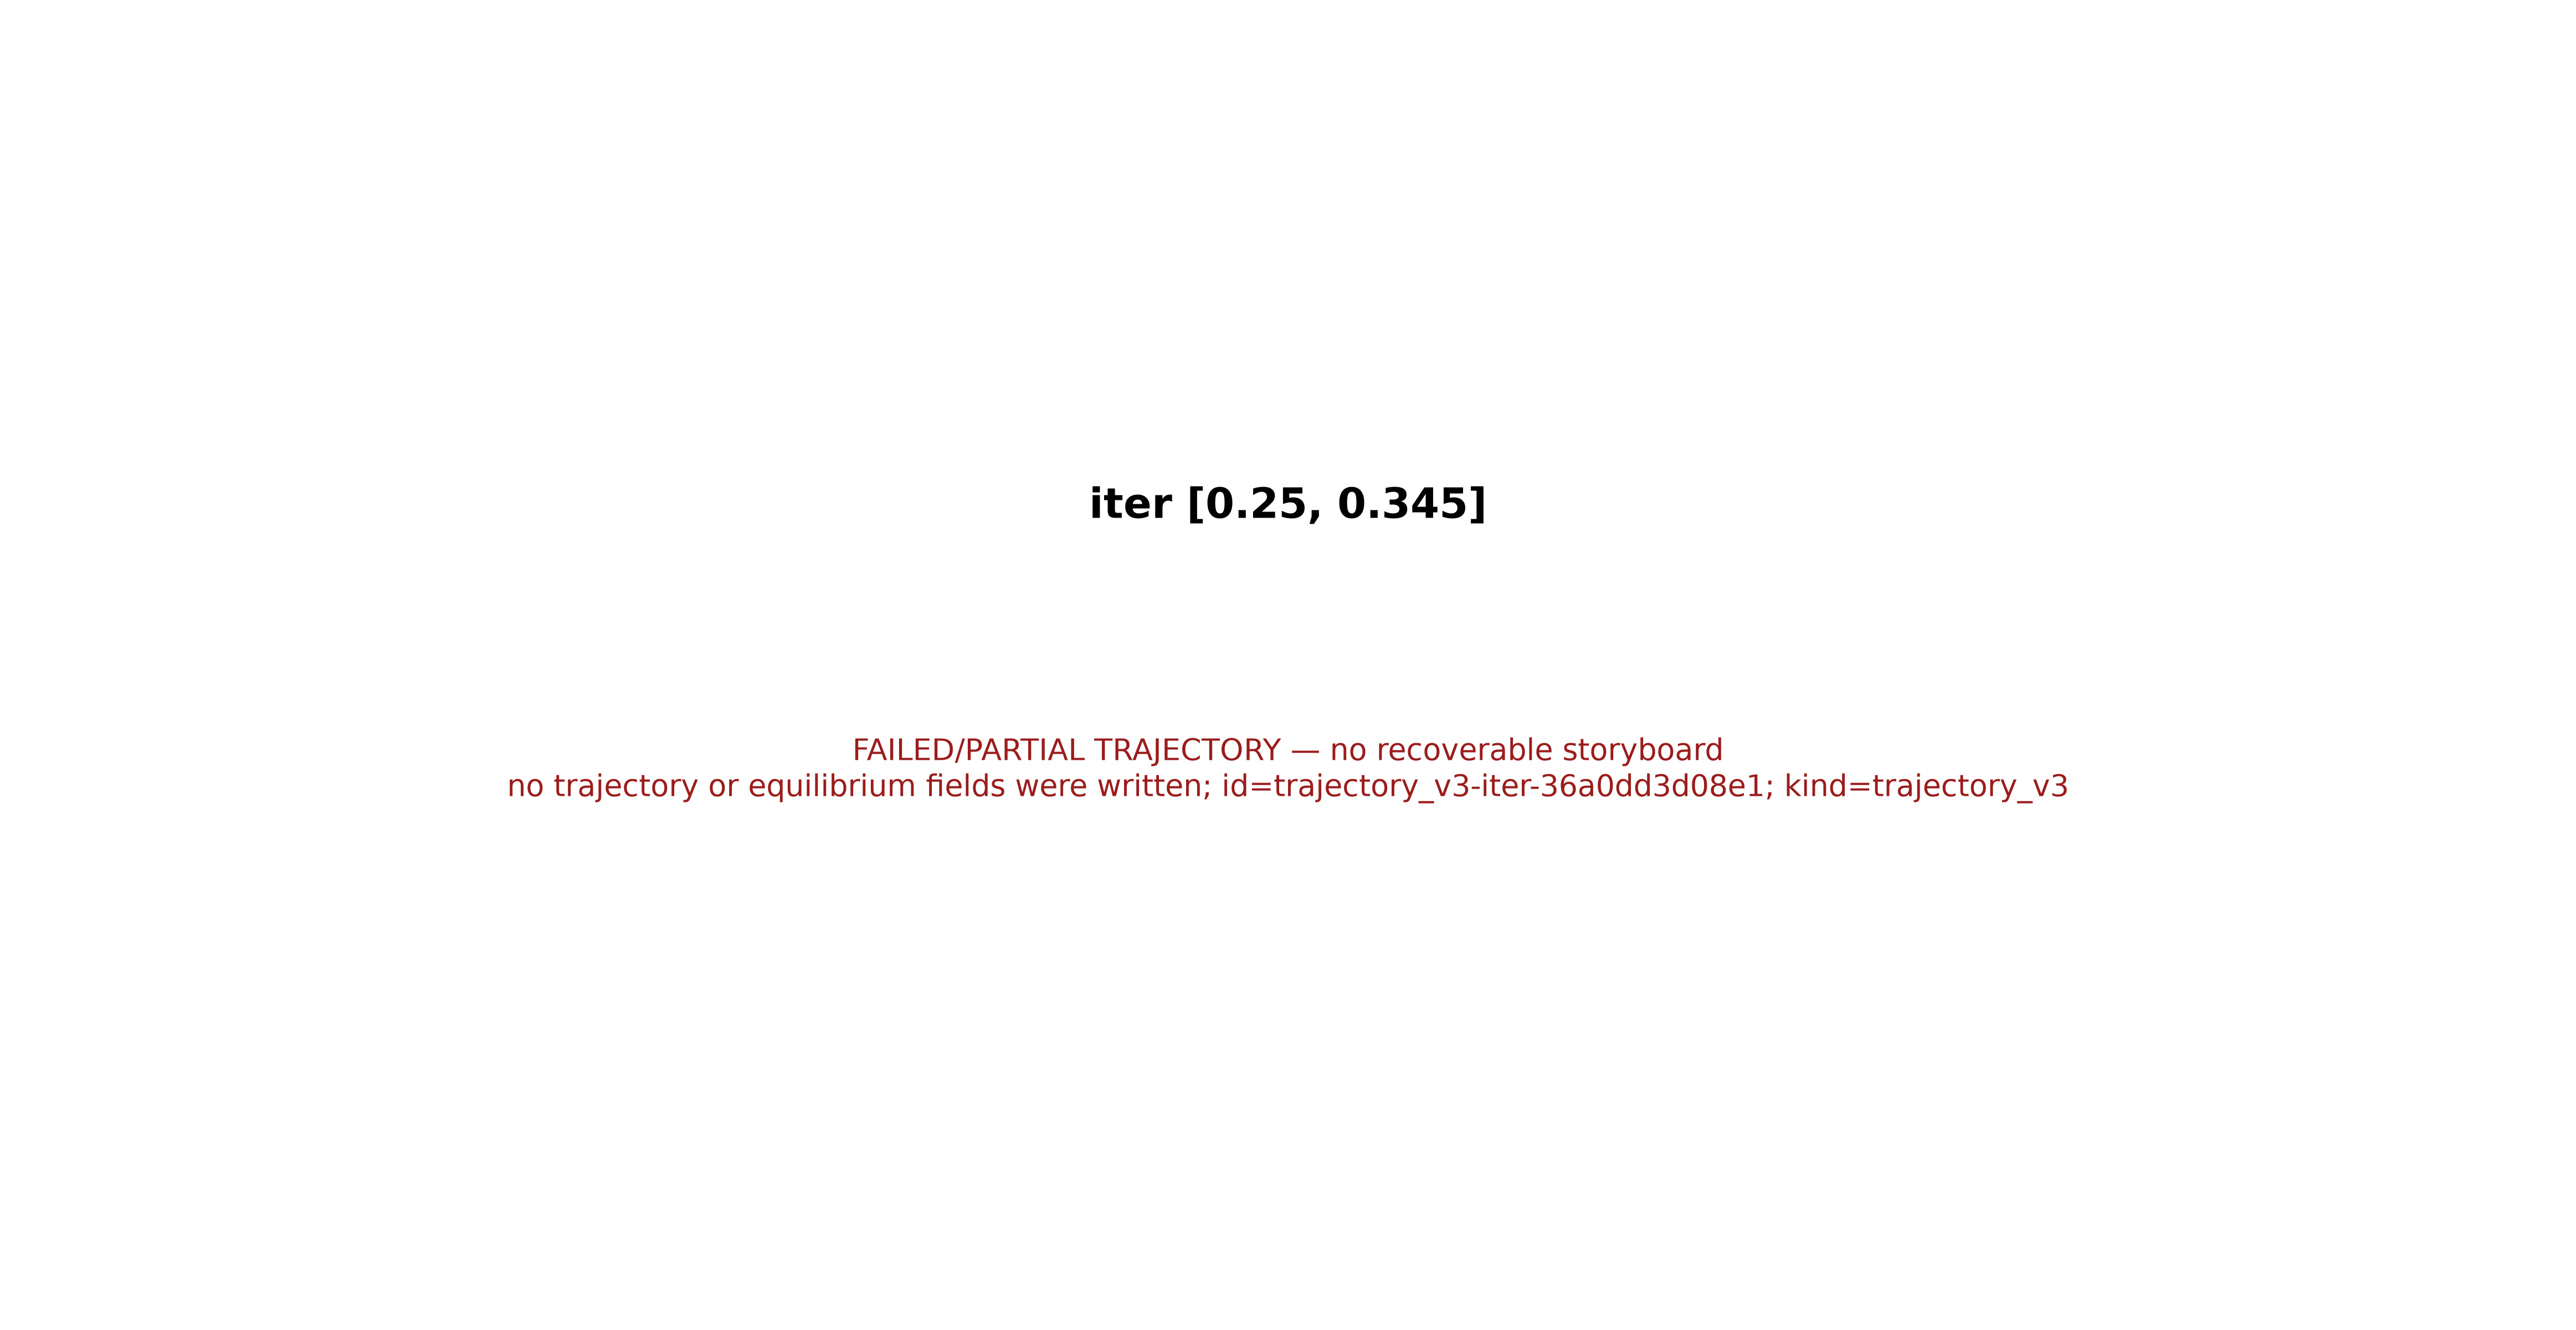
\includegraphics[width=0.88\linewidth]{figures/failed_band_evolution_055_iter_0p25_0p345_trajectory_v3-iter-36a0dd3d08e1.png}
\caption{Supplemental failed/partial trajectory evidence for iter at torsion levels $[0.25,0.345]$ (case trajectory\_v3-iter-36a0dd3d08e1; state=deferred; classification=deferred). The case is retained regardless of PDE or geometric success. Orange dashed curves are the fixed target band and blue solid curves are the moving equilibrium band; when state recovery is impossible, the PNG records the reason. Data status: diagnostic\_only.}
\label{fig:failed-storyboard-trajectory-v3-iter-36a0dd3d08e1}
\end{figure}

\begin{figure}[tbp]
\centering
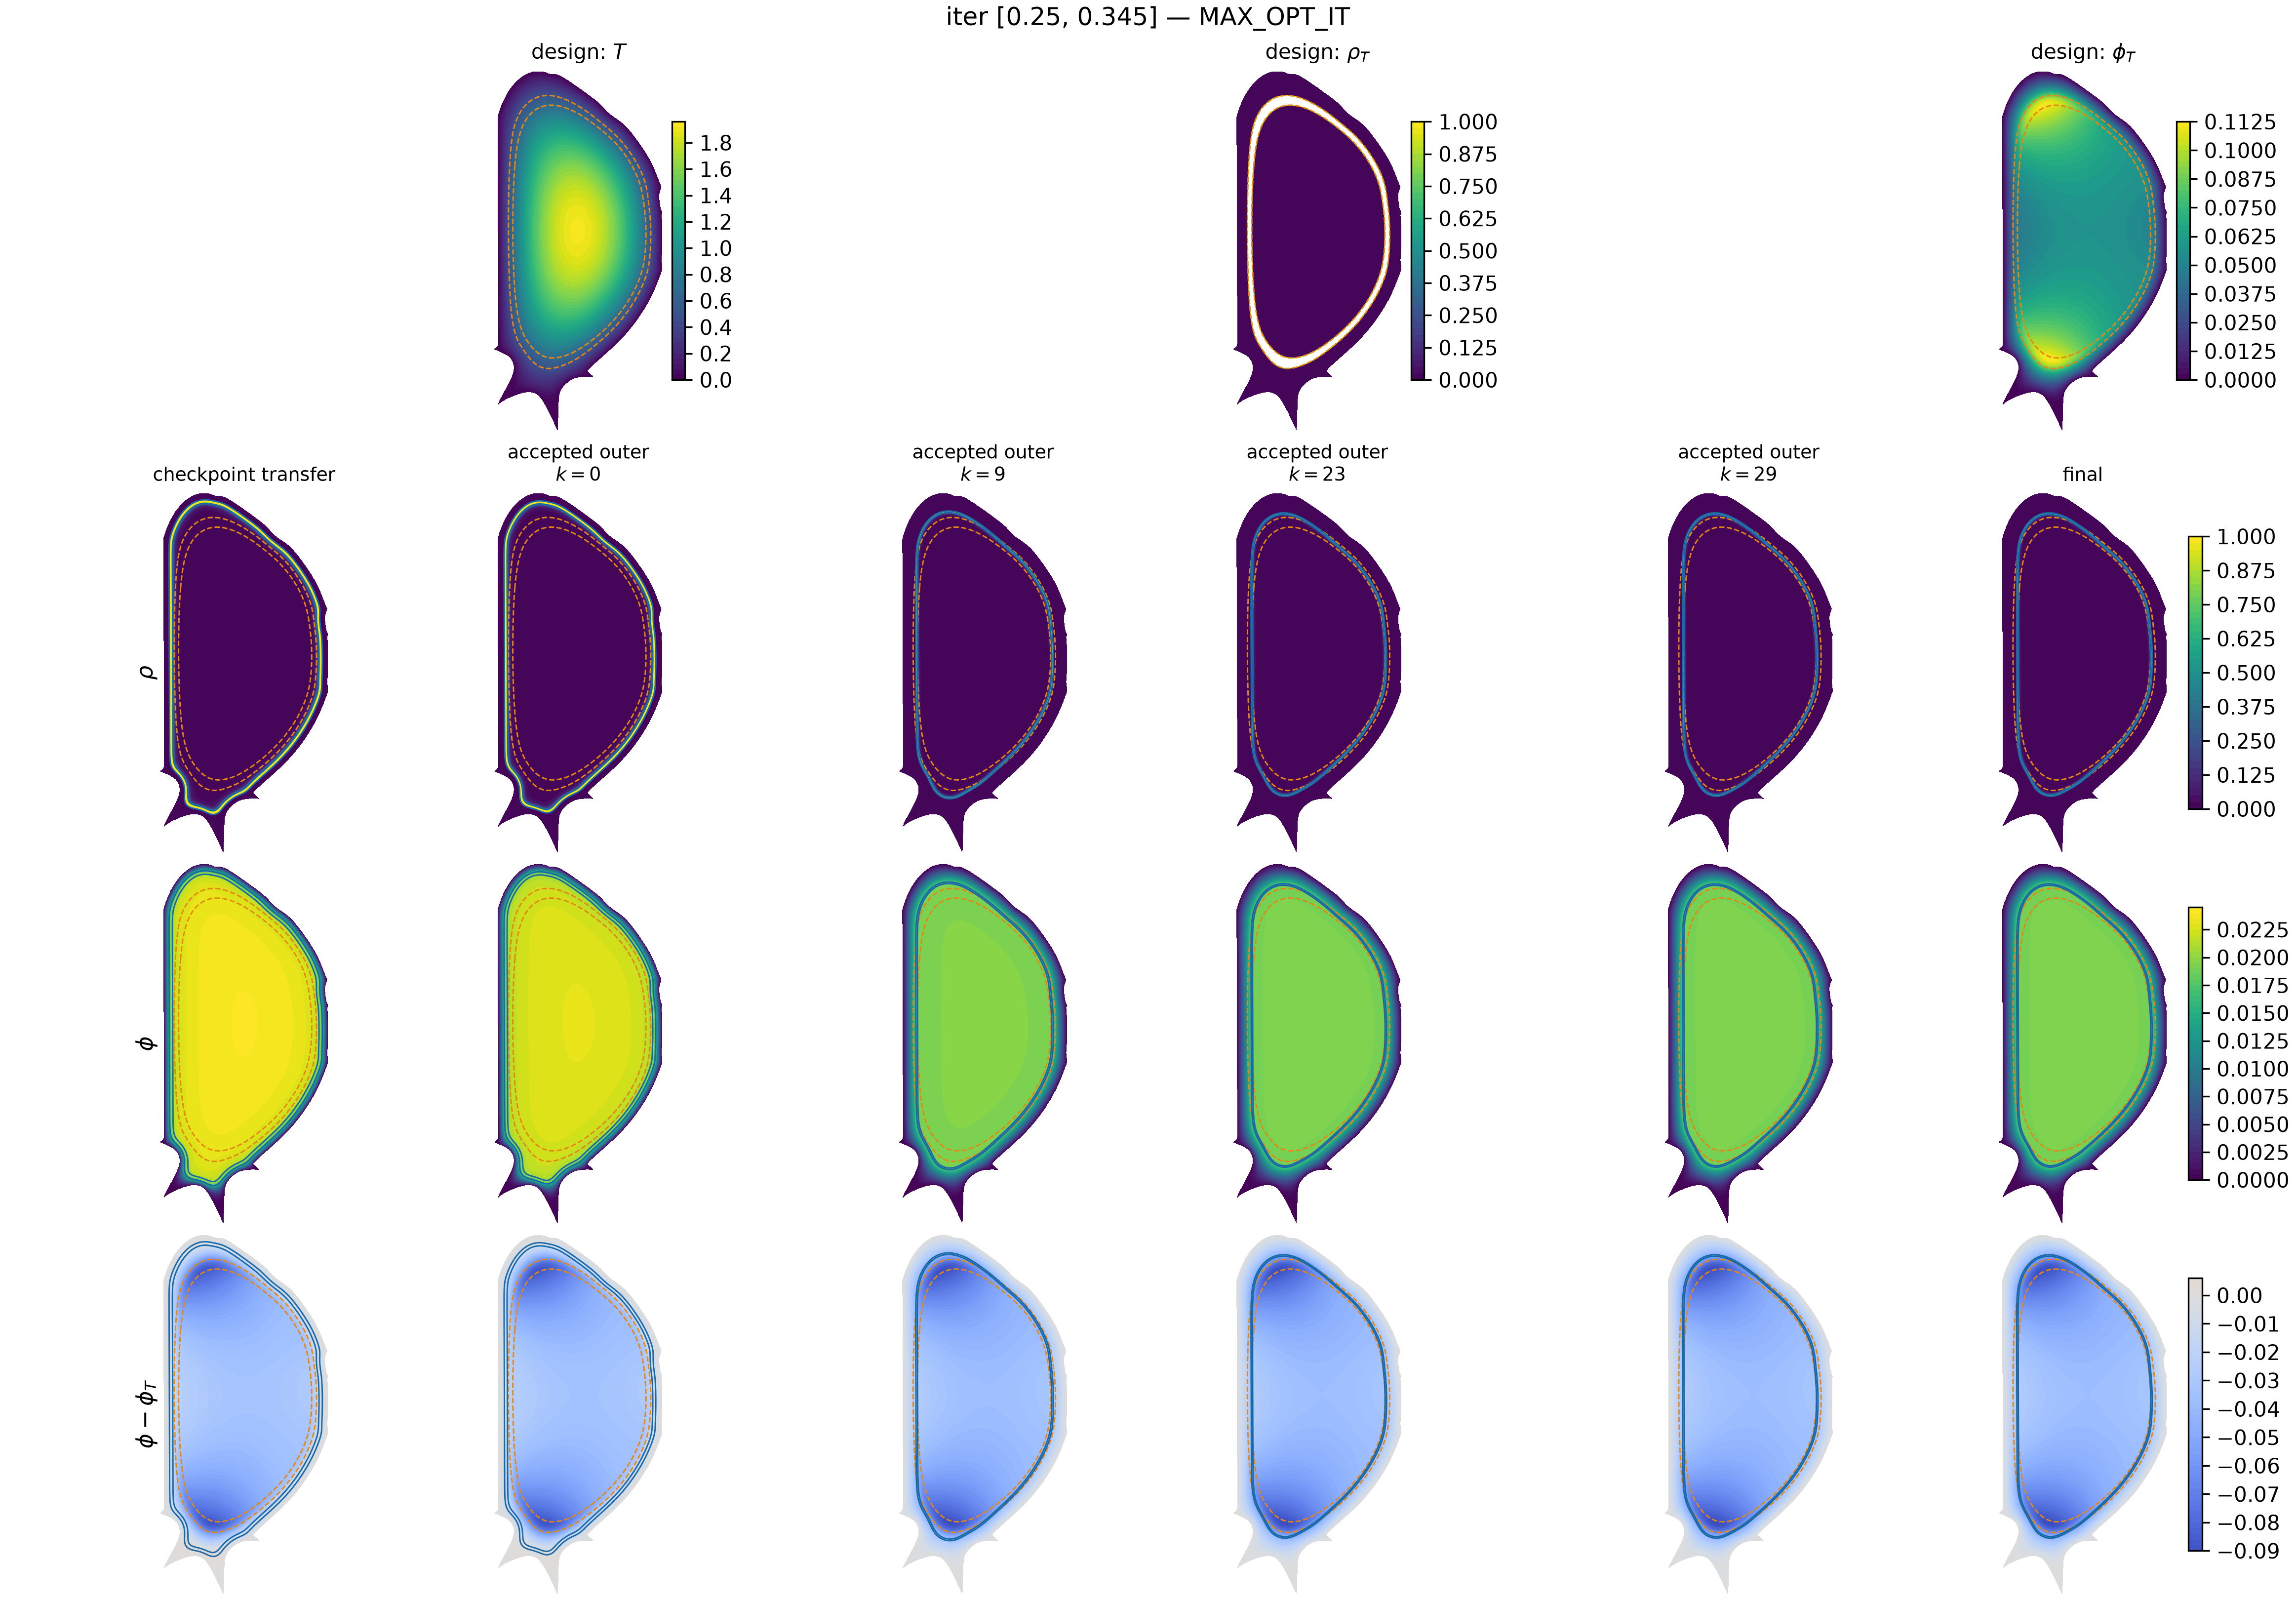
\includegraphics[width=0.88\linewidth]{figures/failed_band_evolution_056_iter_0p25_0p345_trajectory_v3-iter-6c99c035c109.png}
\caption{Supplemental failed/partial trajectory evidence for iter at torsion levels $[0.25,0.345]$ (case trajectory\_v3-iter-6c99c035c109; state=completed; classification=pde\_converged\_with\_capped\_trials). The case is retained regardless of PDE or geometric success. Orange dashed curves are the fixed target band and blue solid curves are the moving equilibrium band; when state recovery is impossible, the PNG records the reason. Data status: actual.}
\label{fig:failed-storyboard-trajectory-v3-iter-6c99c035c109}
\end{figure}

\begin{figure}[tbp]
\centering
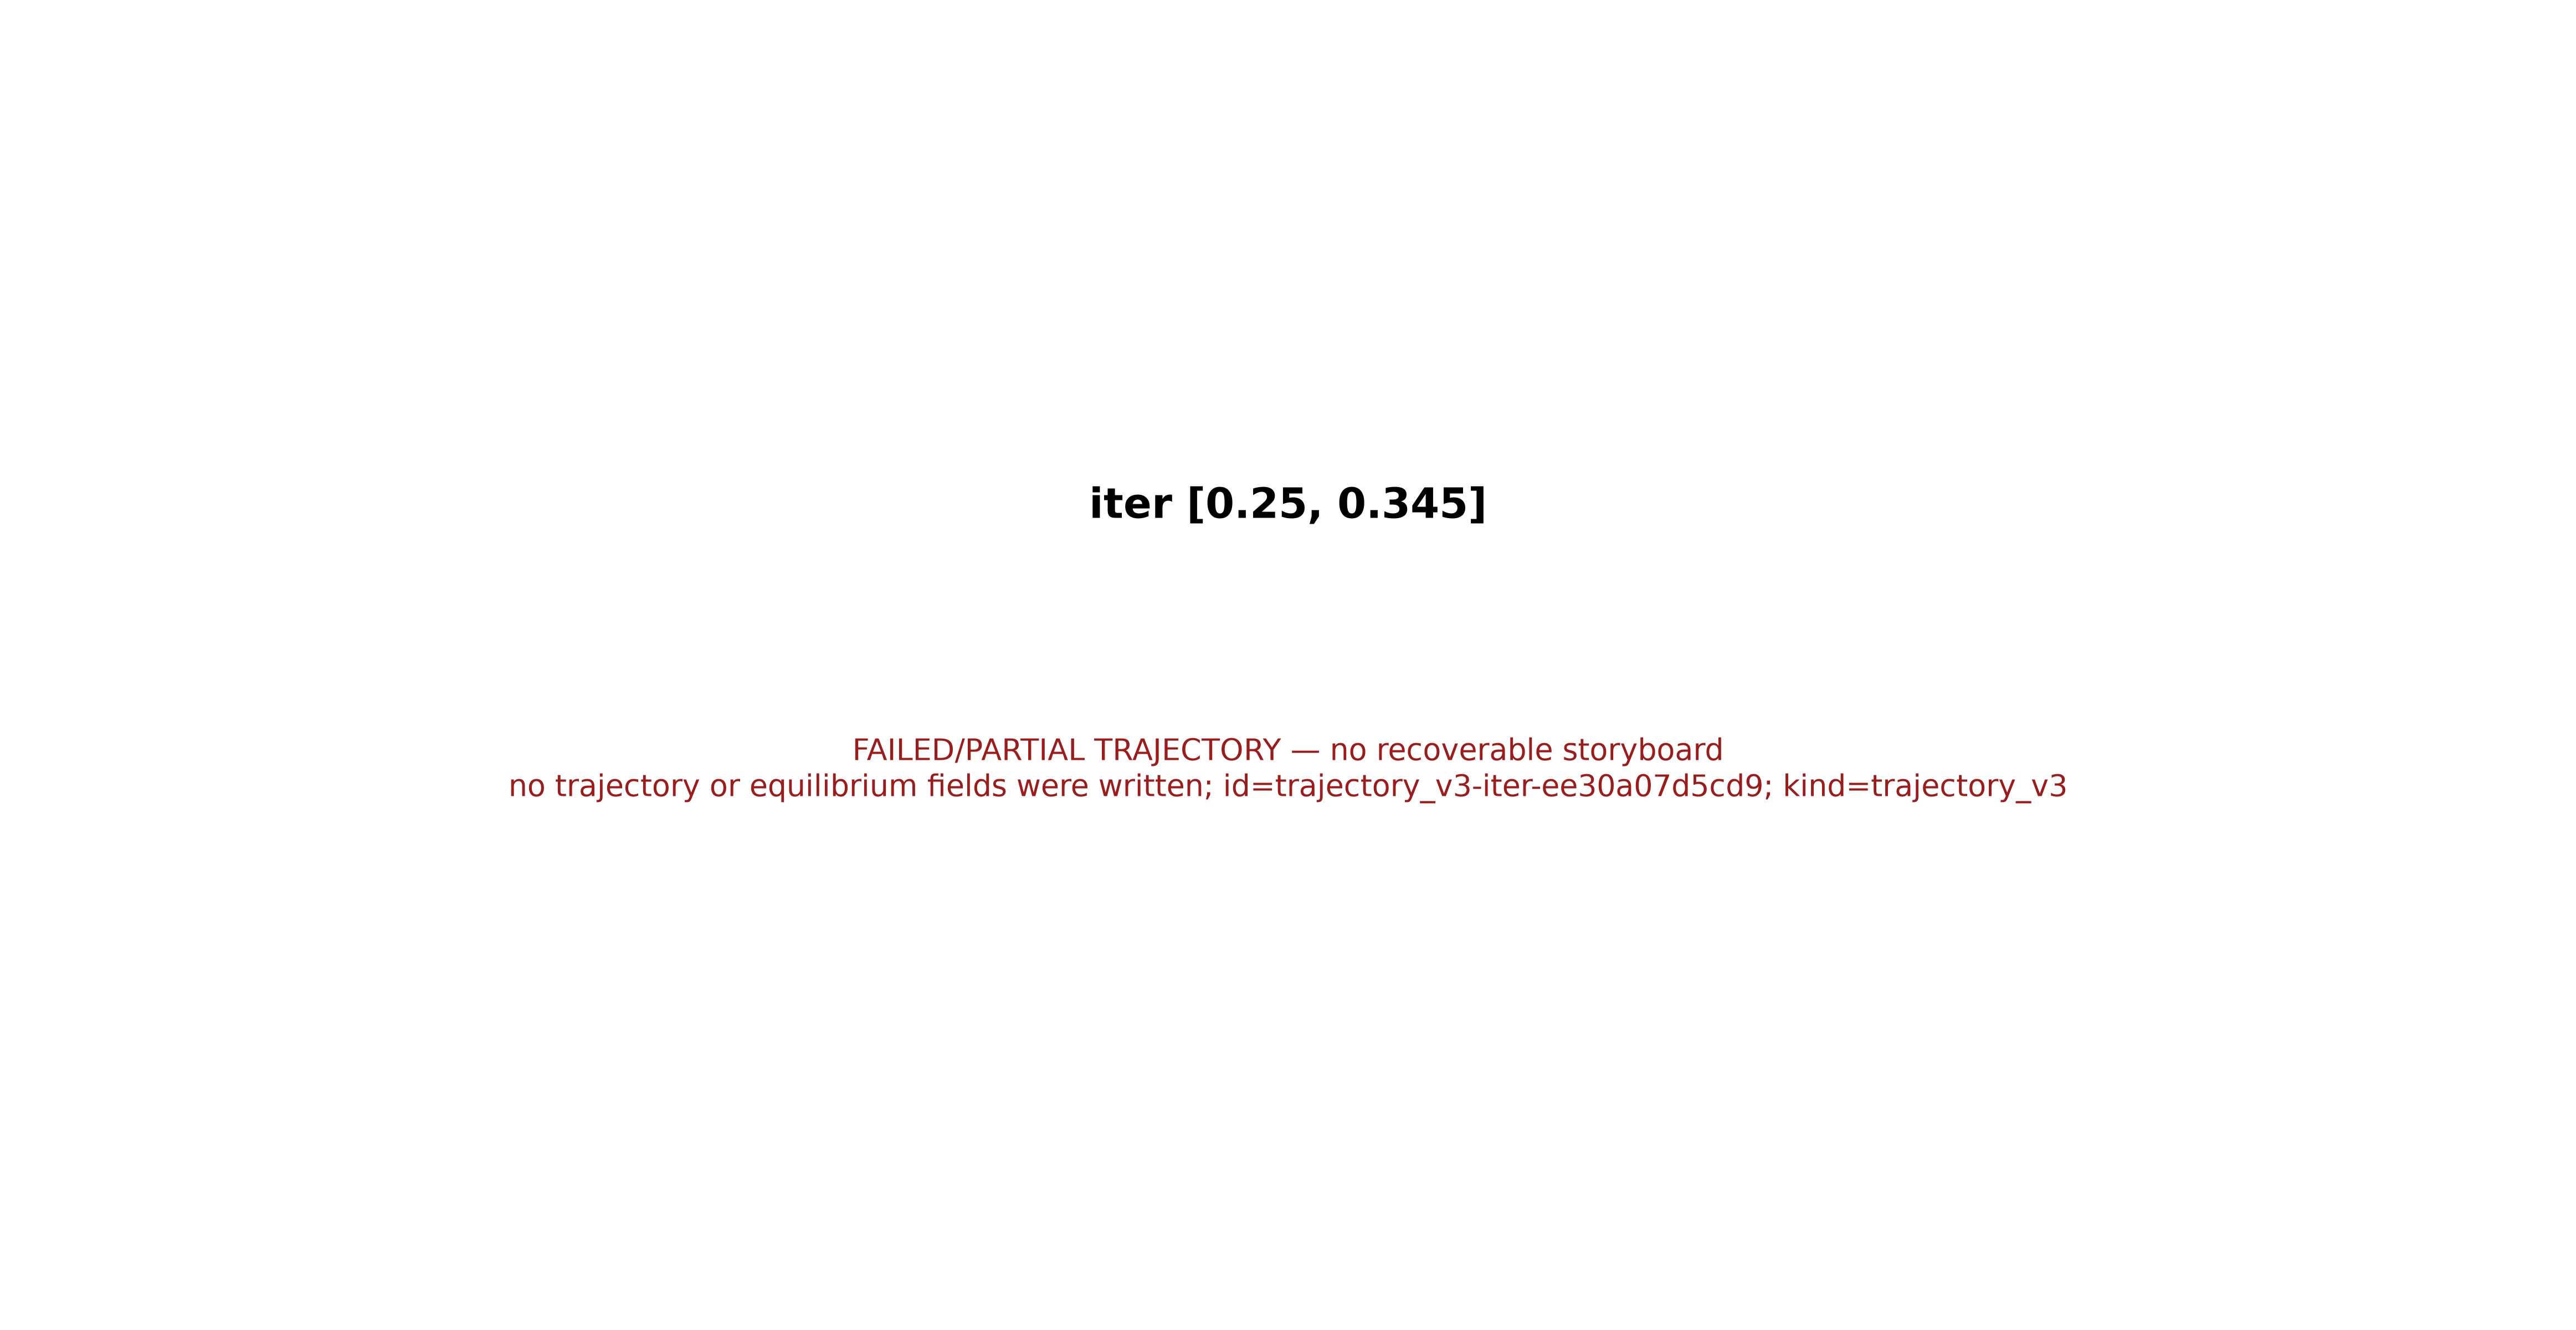
\includegraphics[width=0.88\linewidth]{figures/failed_band_evolution_057_iter_0p25_0p345_trajectory_v3-iter-ee30a07d5cd9.png}
\caption{Supplemental failed/partial trajectory evidence for iter at torsion levels $[0.25,0.345]$ (case trajectory\_v3-iter-ee30a07d5cd9; state=deferred; classification=deferred). The case is retained regardless of PDE or geometric success. Orange dashed curves are the fixed target band and blue solid curves are the moving equilibrium band; when state recovery is impossible, the PNG records the reason. Data status: diagnostic\_only.}
\label{fig:failed-storyboard-trajectory-v3-iter-ee30a07d5cd9}
\end{figure}

\begin{figure}[tbp]
\centering
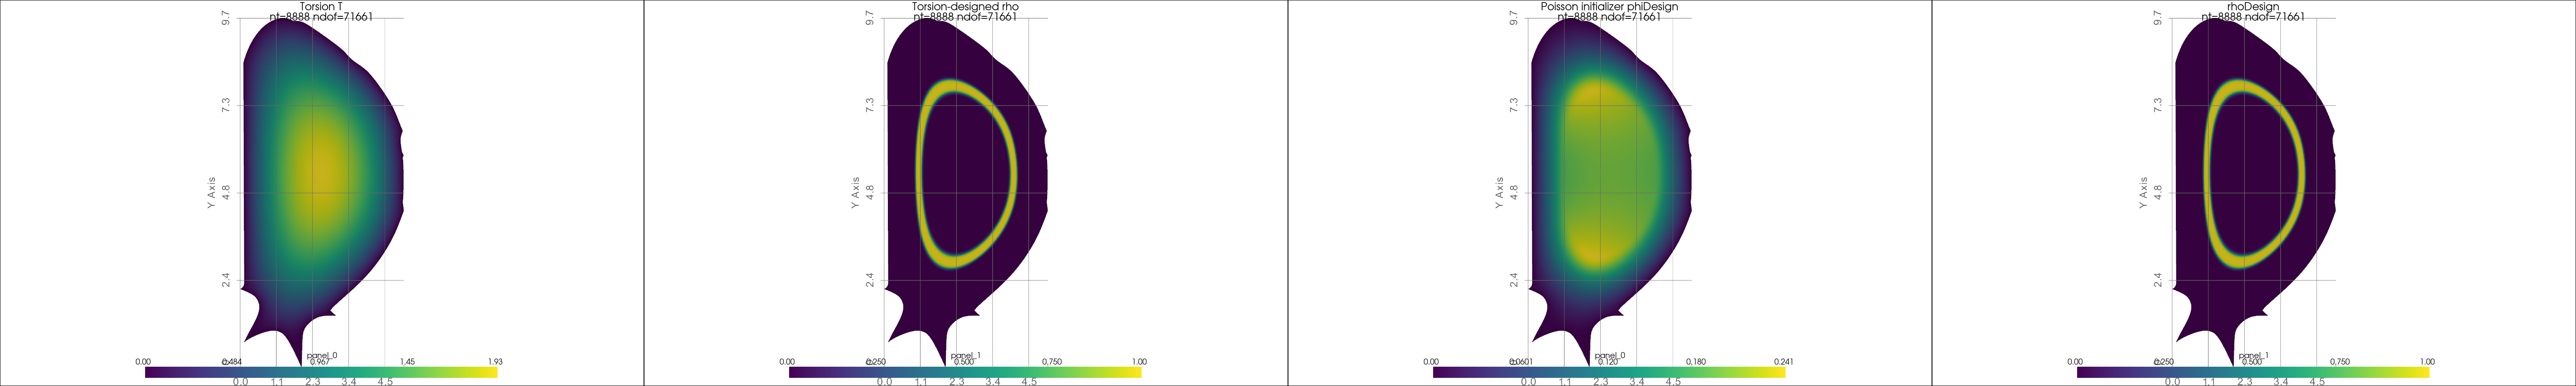
\includegraphics[width=0.88\linewidth]{figures/iter_0p6_0p7_direct_window_fit_design.png}
\caption{Direct fitted-window Newton control for ITER torsion levels $[0.60,0.70]$: target torsion, density, and Poisson-potential design fields, shown once. The P4 mesh has 71,661 global degrees of freedom and the solve uses four-rank MUMPS. Data status: actual.}
\label{fig:direct-window-fit-iter-design}
\end{figure}

\begin{figure}[tbp]
\centering
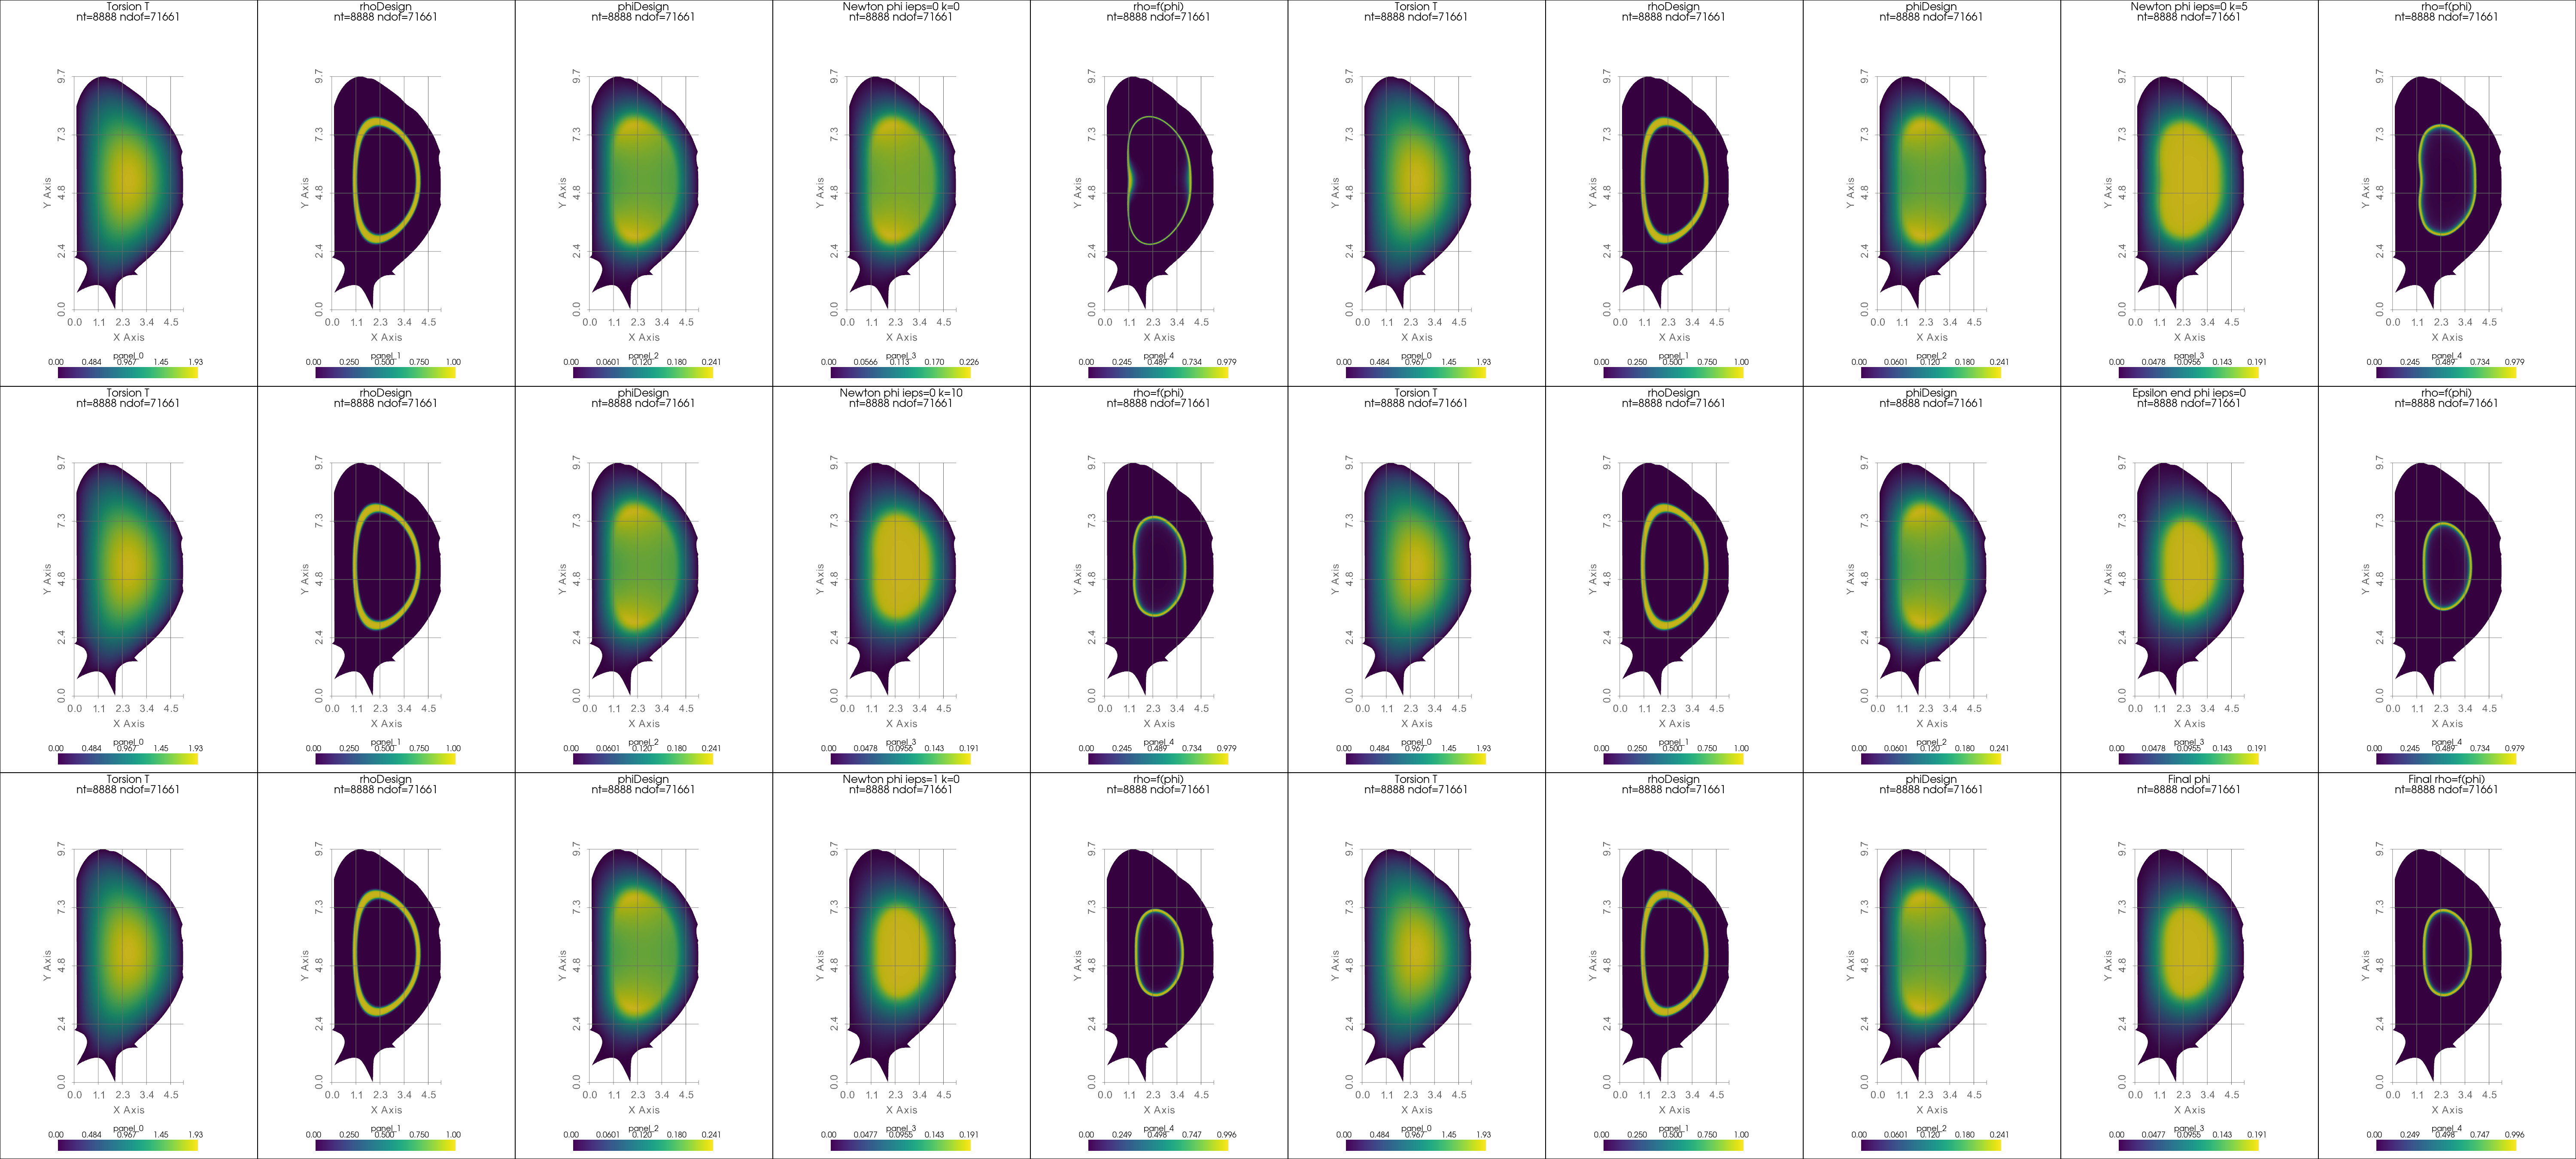
\includegraphics[width=0.88\linewidth]{figures/iter_0p6_0p7_direct_window_fit_storyboard.png}
\caption{Direct fitted-window Newton evolution for ITER torsion levels $[0.60,0.70]$ at continuation ratios $0.11$ and $0.08$. Complete MPI fields are gathered on rank zero and rendered without mesh edges. This is failed evidence: the two stages ended after repeated line-search rejection at residuals $2.9613\times10^{-2}$ and $2.9678\times10^{-2}$, respectively, before the 160-iteration cap. Data status: failed\_evidence.}
\label{fig:direct-window-fit-iter-storyboard}
\end{figure}

\begin{figure}[tbp]
\centering
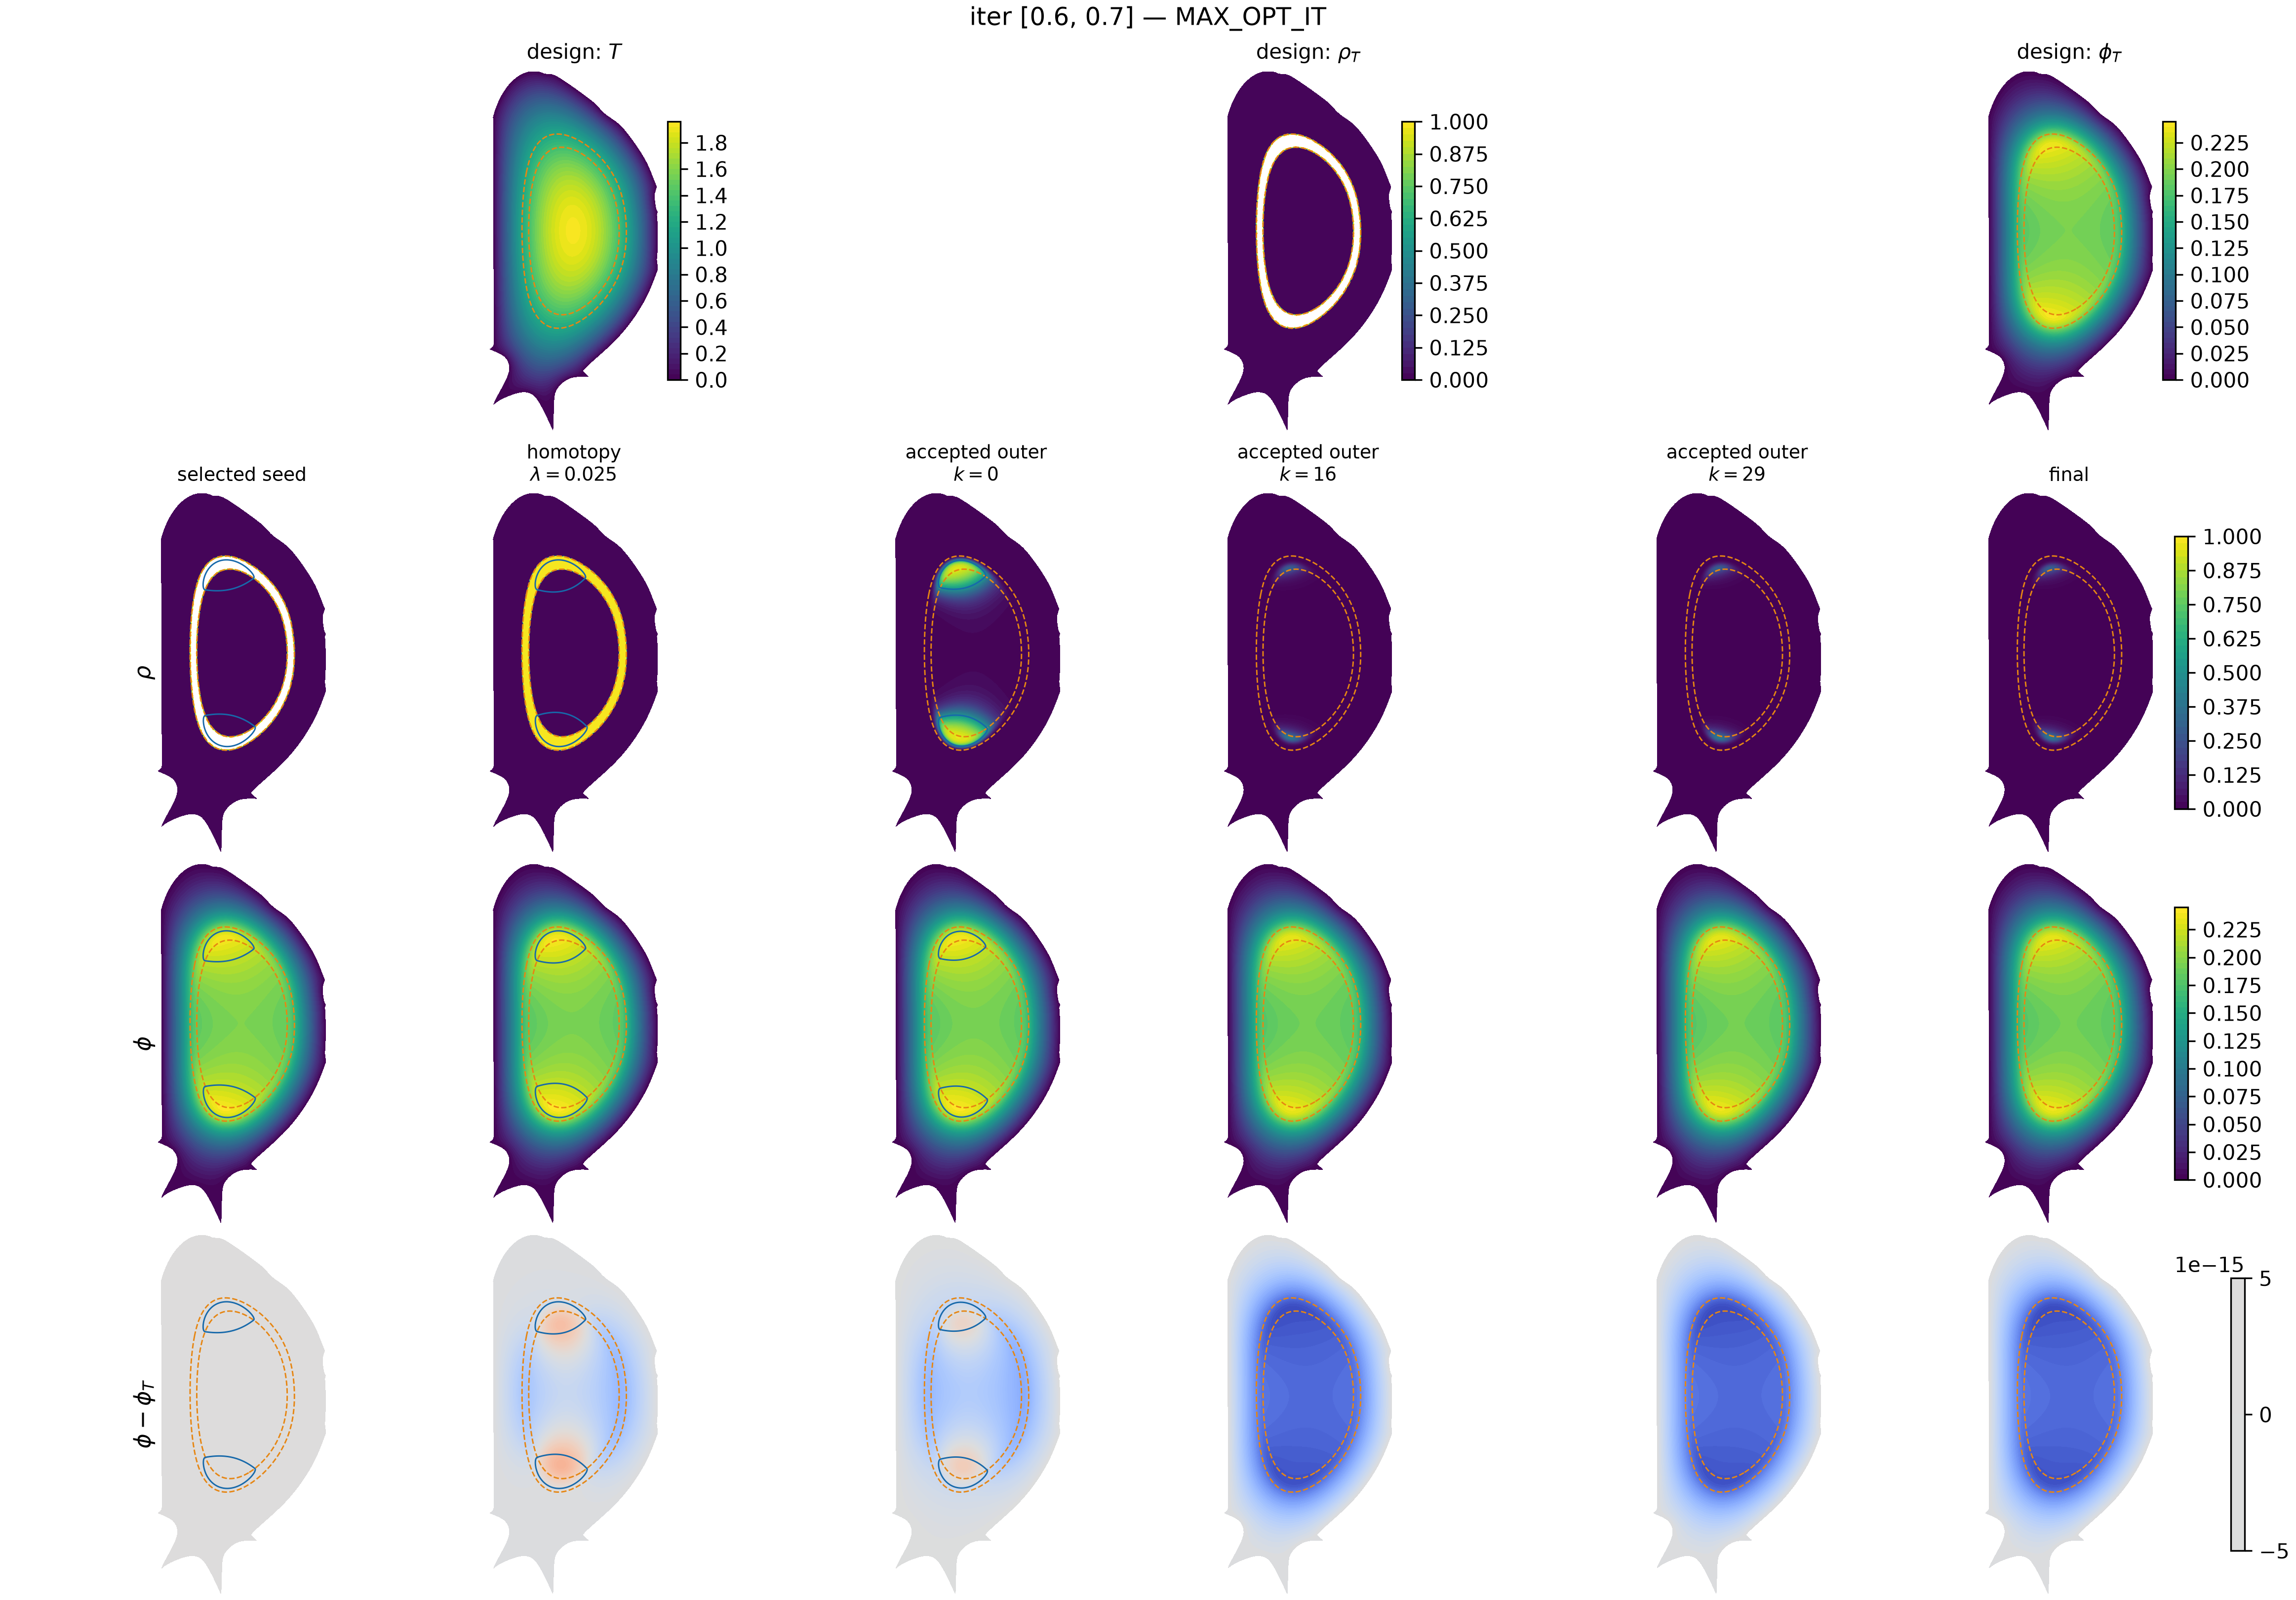
\includegraphics[width=0.88\linewidth]{figures/iter_0p6_0p7_early_threshold_lambda_0p025_storyboard.png}
\caption{ITER [0.6,0.7] early threshold release at fixed source-homotopy lambda=0.025: two continuation Newton iterations reached 1.67e-14, while 30 reduced steps ended at residual 8.86e-14, relative leakage 2.002e-2, relative missing area 9.757e-1, and zero certified area. Data status: actual; partial-homotopy PDE-converged, geometrically unsuccessful.}
\label{fig:iter-early-threshold-lambda-0025}
\end{figure}

\begin{figure}[tbp]
\centering
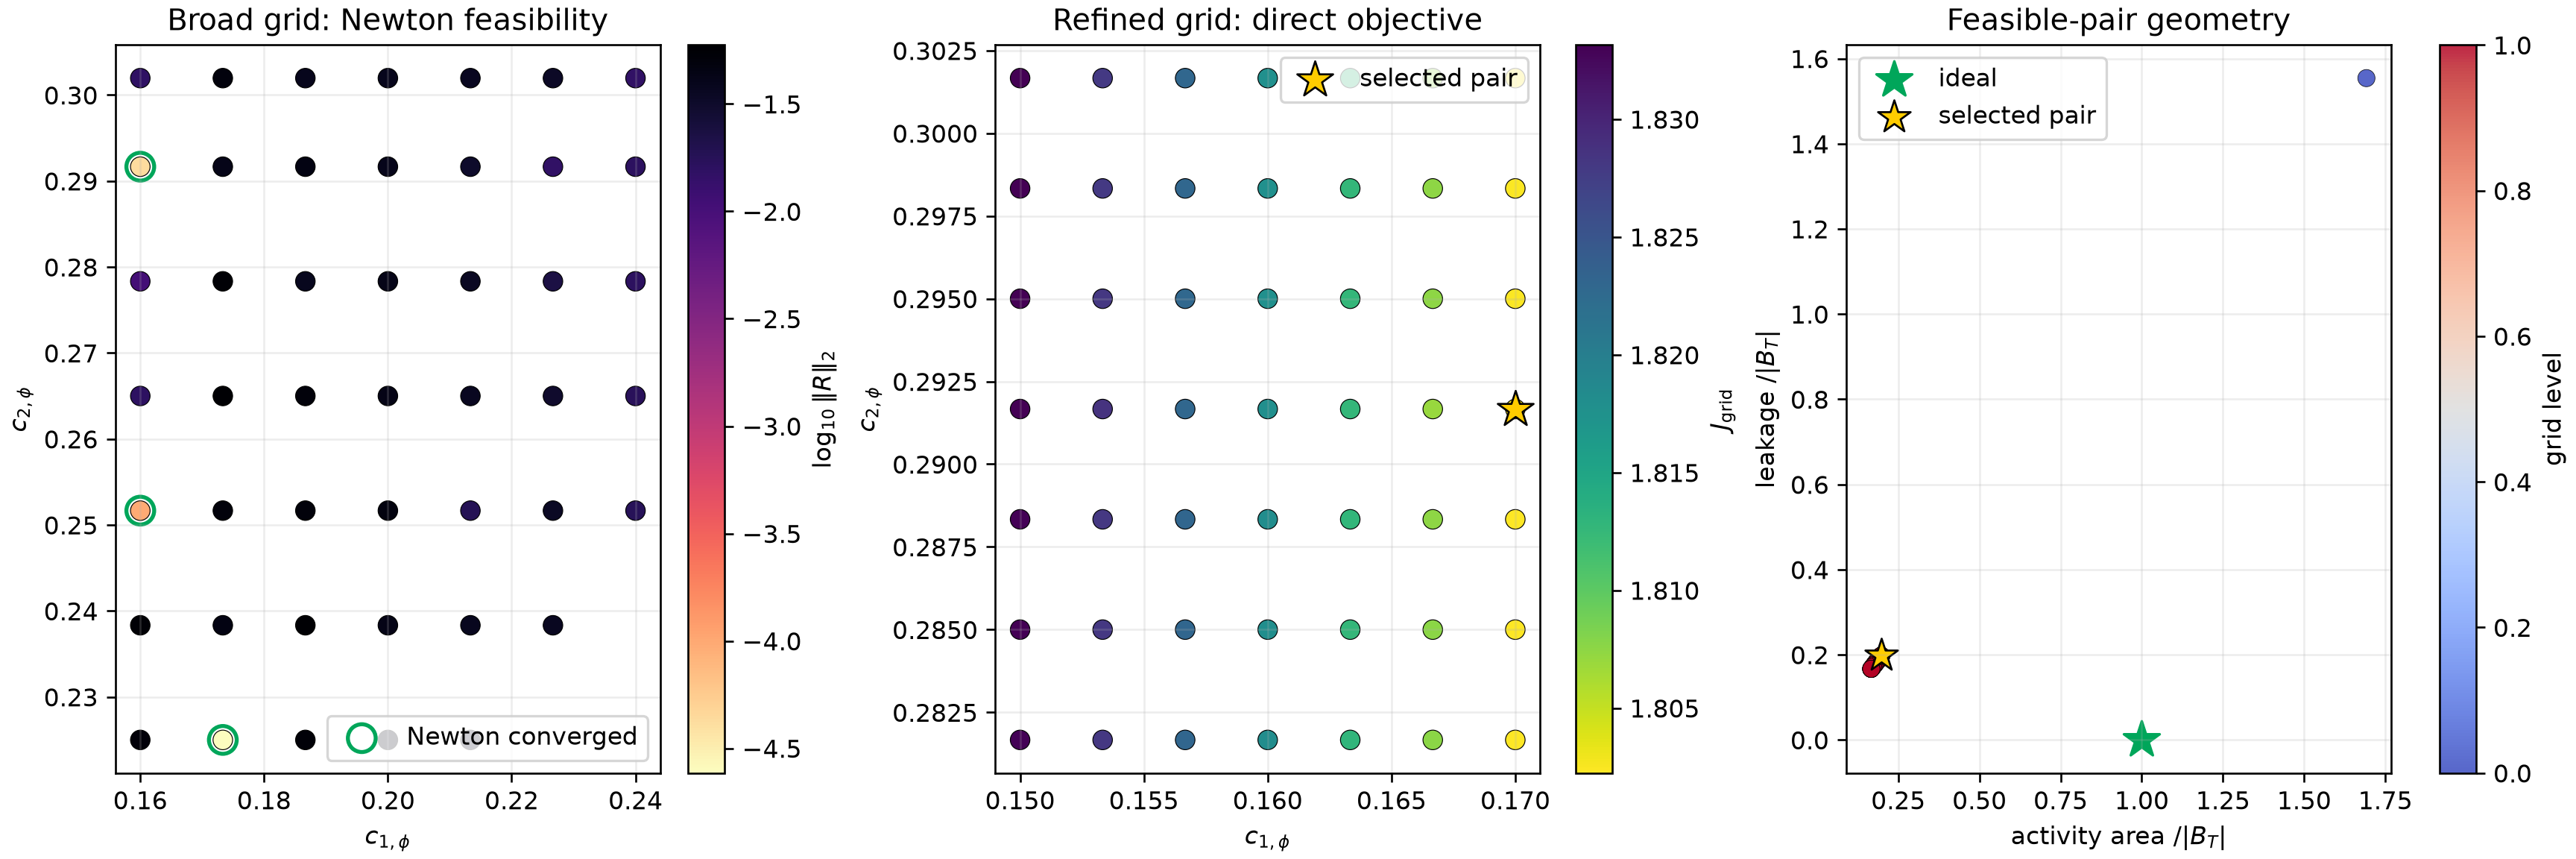
\includegraphics[width=0.97\linewidth]{figures/iter_0p6_0p7_bruteforce_grid_search.png}
\caption{MPI-split brute-force threshold search for sharp-target ITER [0.6,0.7] with epsPhi/(c2Phi-c1Phi)=0.04. Five four-rank MUMPS groups evaluated 95 threshold pairs at Newton tolerance 1e-4: 3 of 46 broad-grid pairs and all 49 continuation-refined pairs converged. The selected pair was (0.1700,0.29167), with residual 2.42e-7, relative leakage 0.1978, and relative activity area 0.1978. Data status: actual; PDE-feasible initialization, geometrically unsuccessful.}
\label{fig:iter-bruteforce-grid-search}
\end{figure}

\clearpage

\begin{figure}[tbp]
\centering
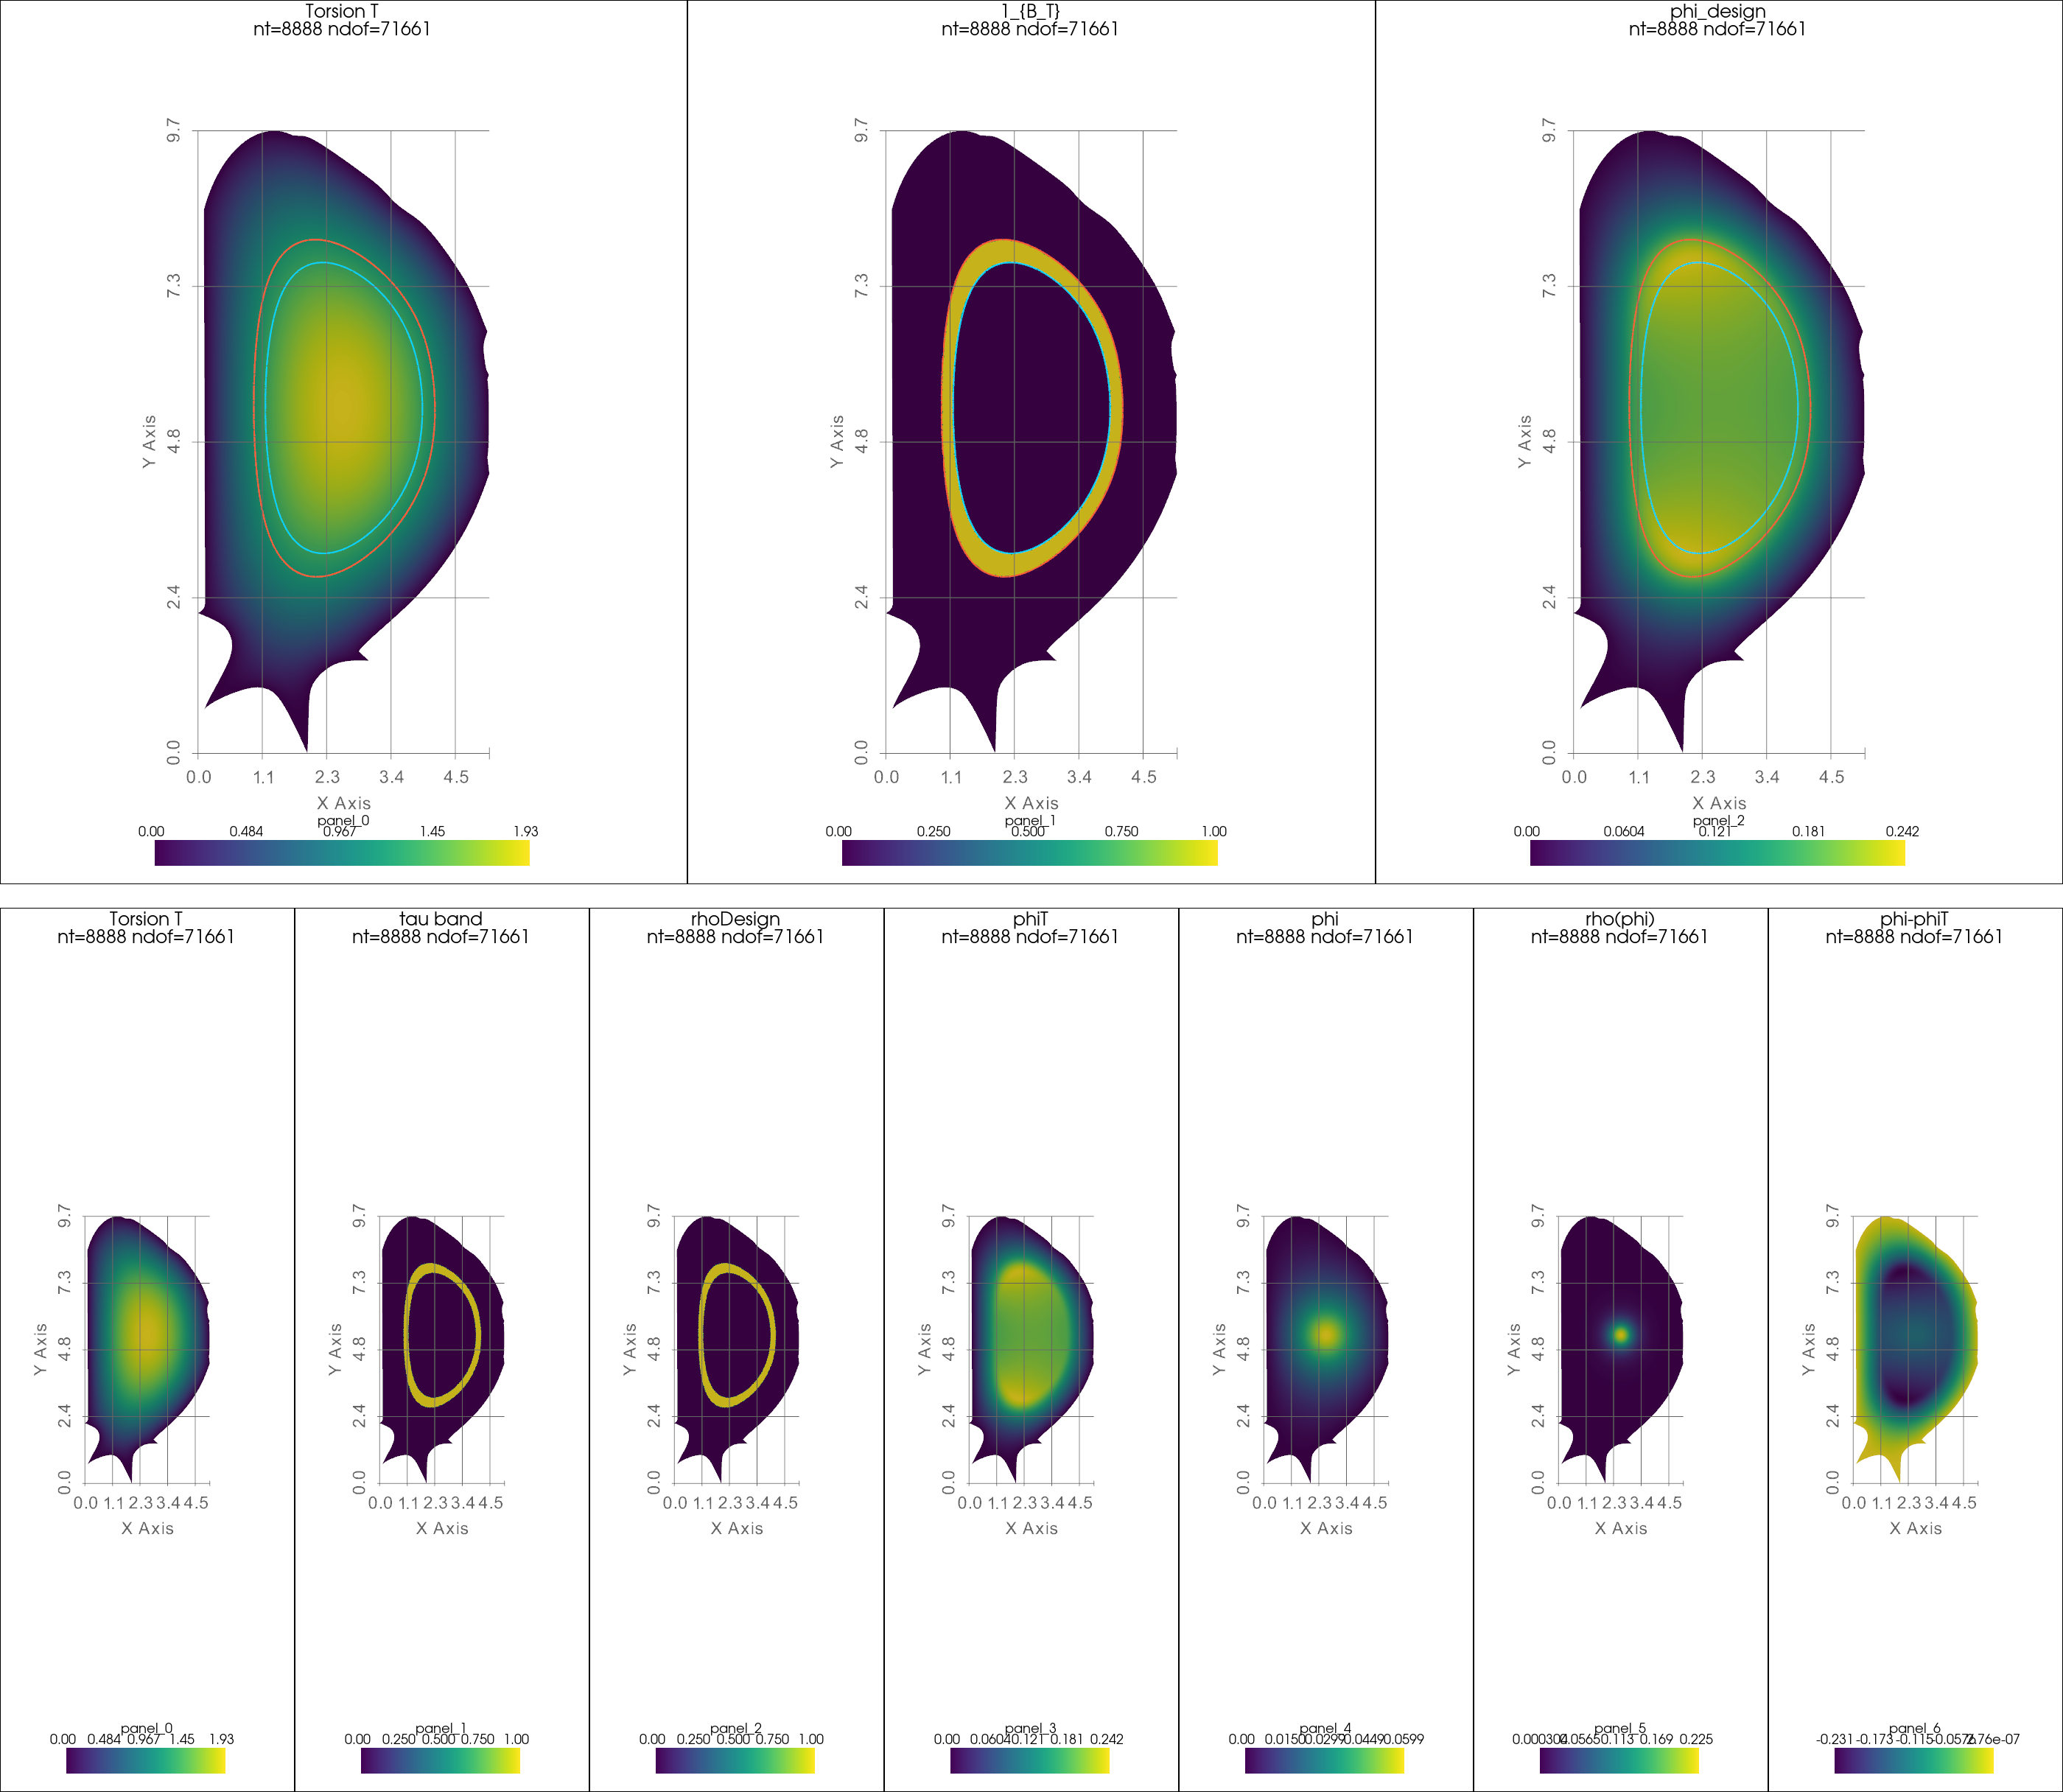
\includegraphics[width=0.97\linewidth]{figures/iter_0p6_0p7_bruteforce_sharp_eps004_storyboard.png}
\caption{Separated design and final fields for the sharp-target ITER brute-force initialization. The upper row contains the target design once; the lower row contains the final reduced-optimization state. Rank zero gathered all 8888 cells and 71661 P4 degrees of freedom, and element edges are hidden. The final exact residual is 2.07e-15, but relative leakage and missing area are 0.0752 and 0.9981, with zero certified area. Data status: actual; final PDE-converged, threshold-space step stagnation.}
\label{fig:iter-bruteforce-sharp-storyboard}
\end{figure}

\begin{landscape}
\begin{figure}[tbp]
\centering
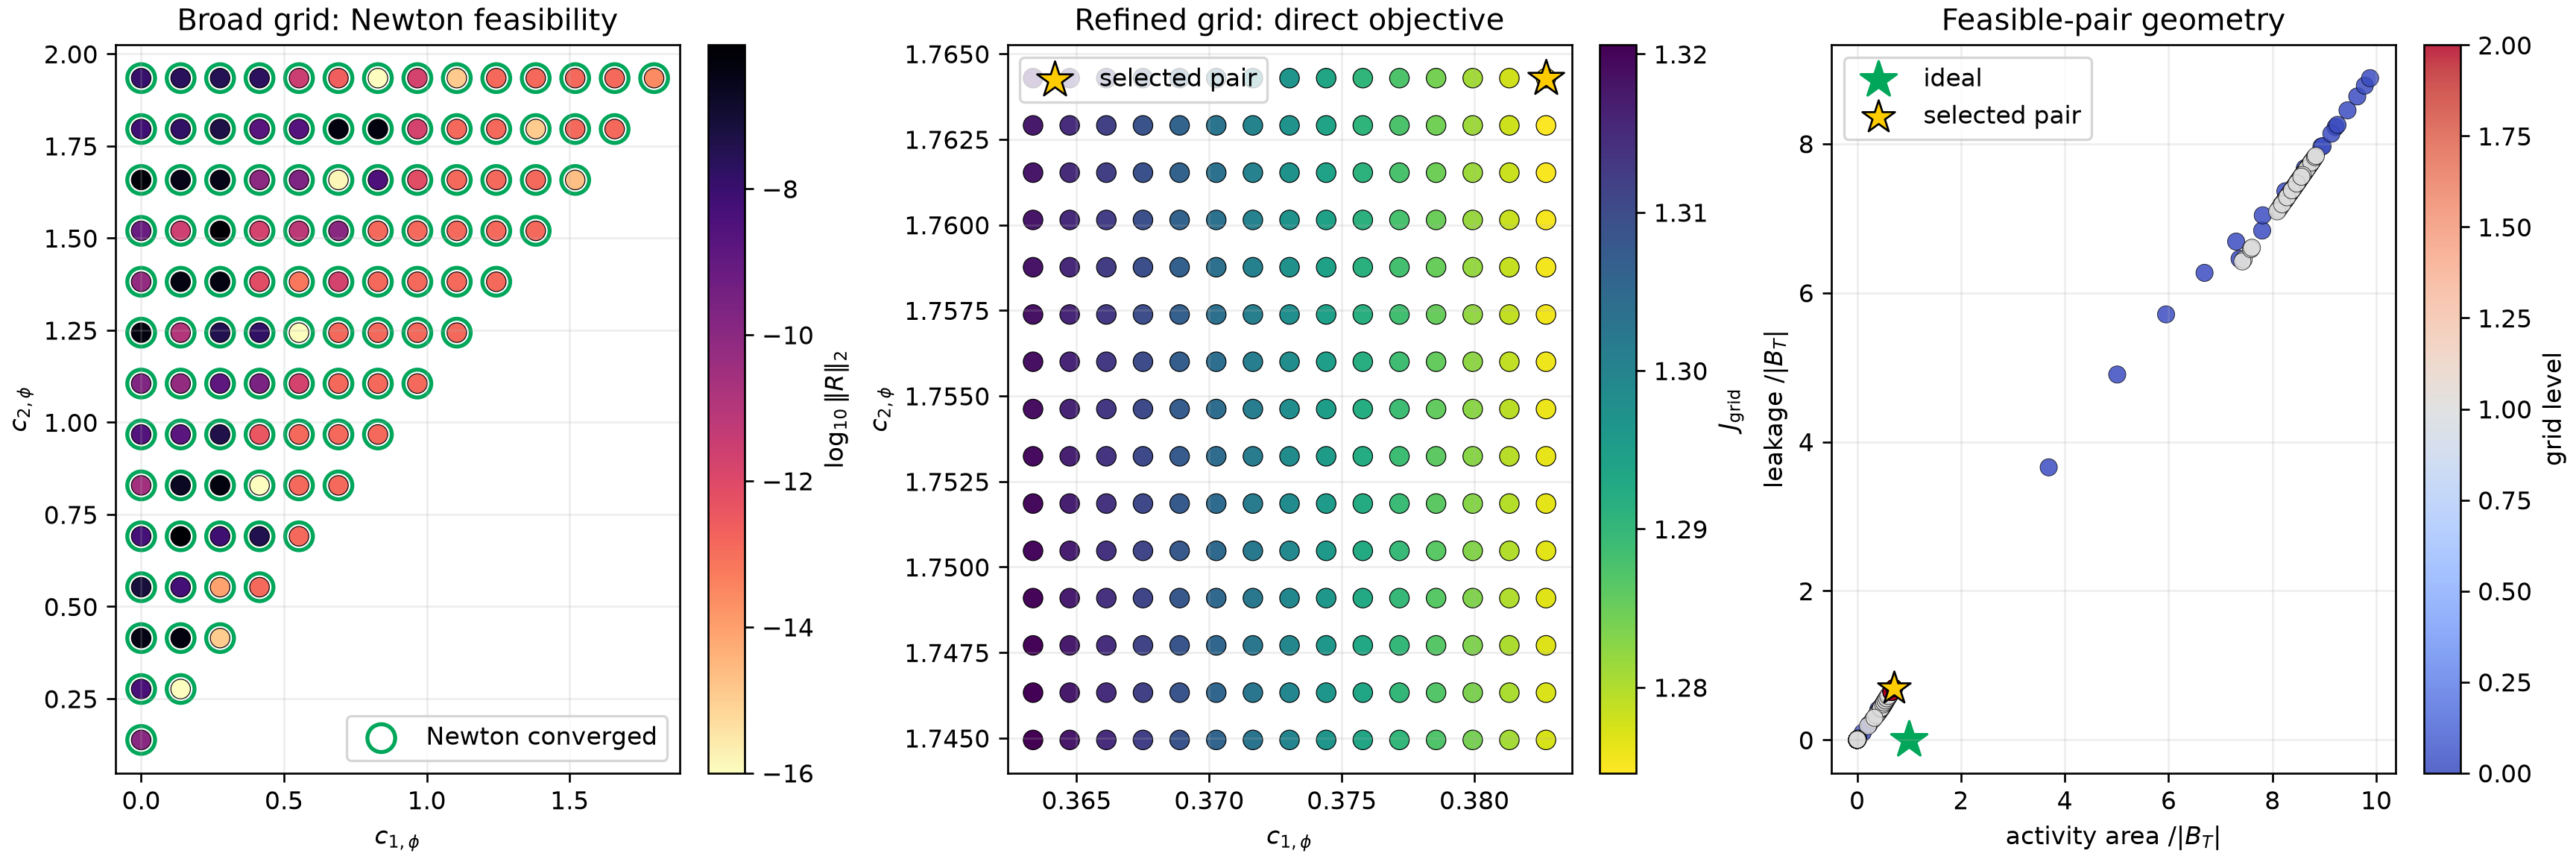
\includegraphics[width=0.97\linewidth]{figures/iter_0p6_0p7_torsion_cap_fine_grid_search.png}
\caption{Expanded physical-cap search for sharp-target ITER [0.6,0.7]. The broad triangle and two 15-by-15 refinements evaluated 555 threshold pairs and 1660 independently seeded Newton branches at tolerance 1e-6. The selected pair (0.3827000,1.7642896) reached residual 9.82e-11, but lies on both upper boundaries of the final refinement. Data status: actual; 555 PDE-feasible pairs, boundary-limited initializer.}
\label{fig:iter-torsion-cap-grid-search}
\end{figure}
\end{landscape}

\begin{landscape}
\begin{figure}[tbp]
\centering
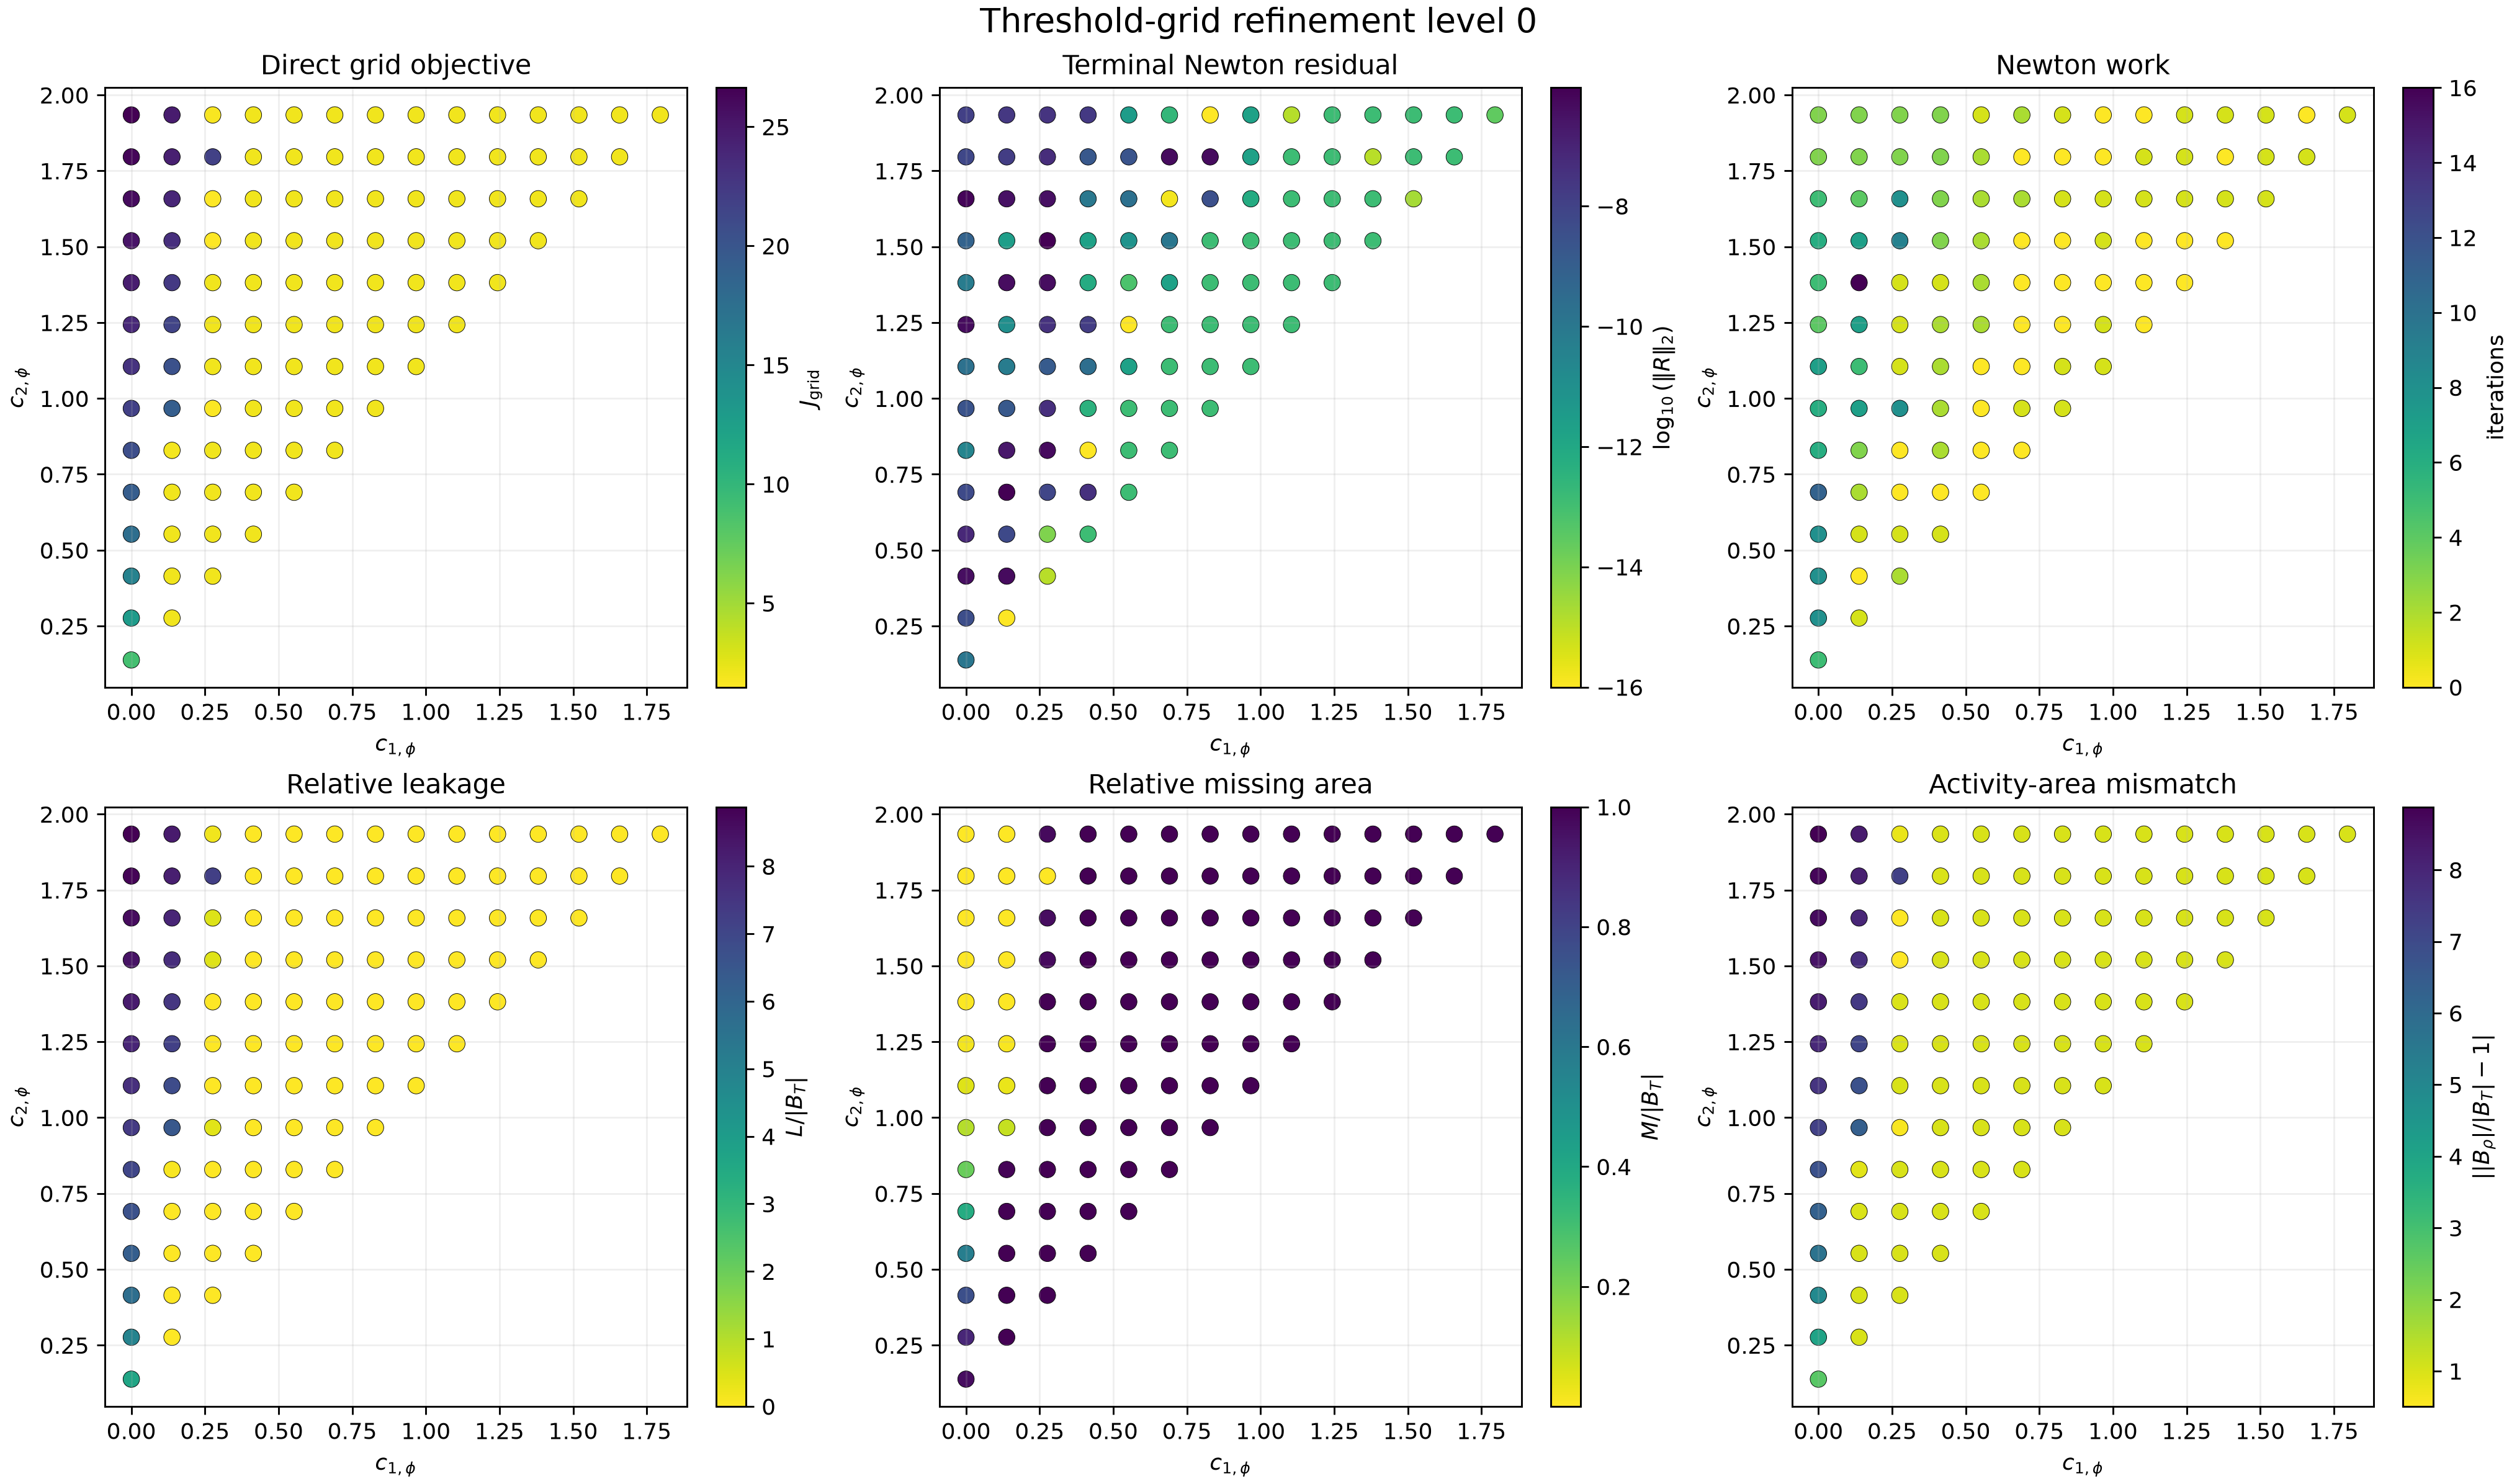
\includegraphics[width=0.97\linewidth]{figures/iter_0p6_0p7_torsion_cap_fine_grid_level_0.png}
\caption{Broad-grid objective, Newton residual and work, leakage, missing area, and activity-area mismatch over 0 <= c1Phi < c2Phi <= max(T). All 105 pairs possess at least one converged, bound-respecting branch. Data status: actual; full physical search triangle.}
\label{fig:iter-torsion-cap-grid-level-0}
\end{figure}
\end{landscape}

\begin{landscape}
\begin{figure}[tbp]
\centering
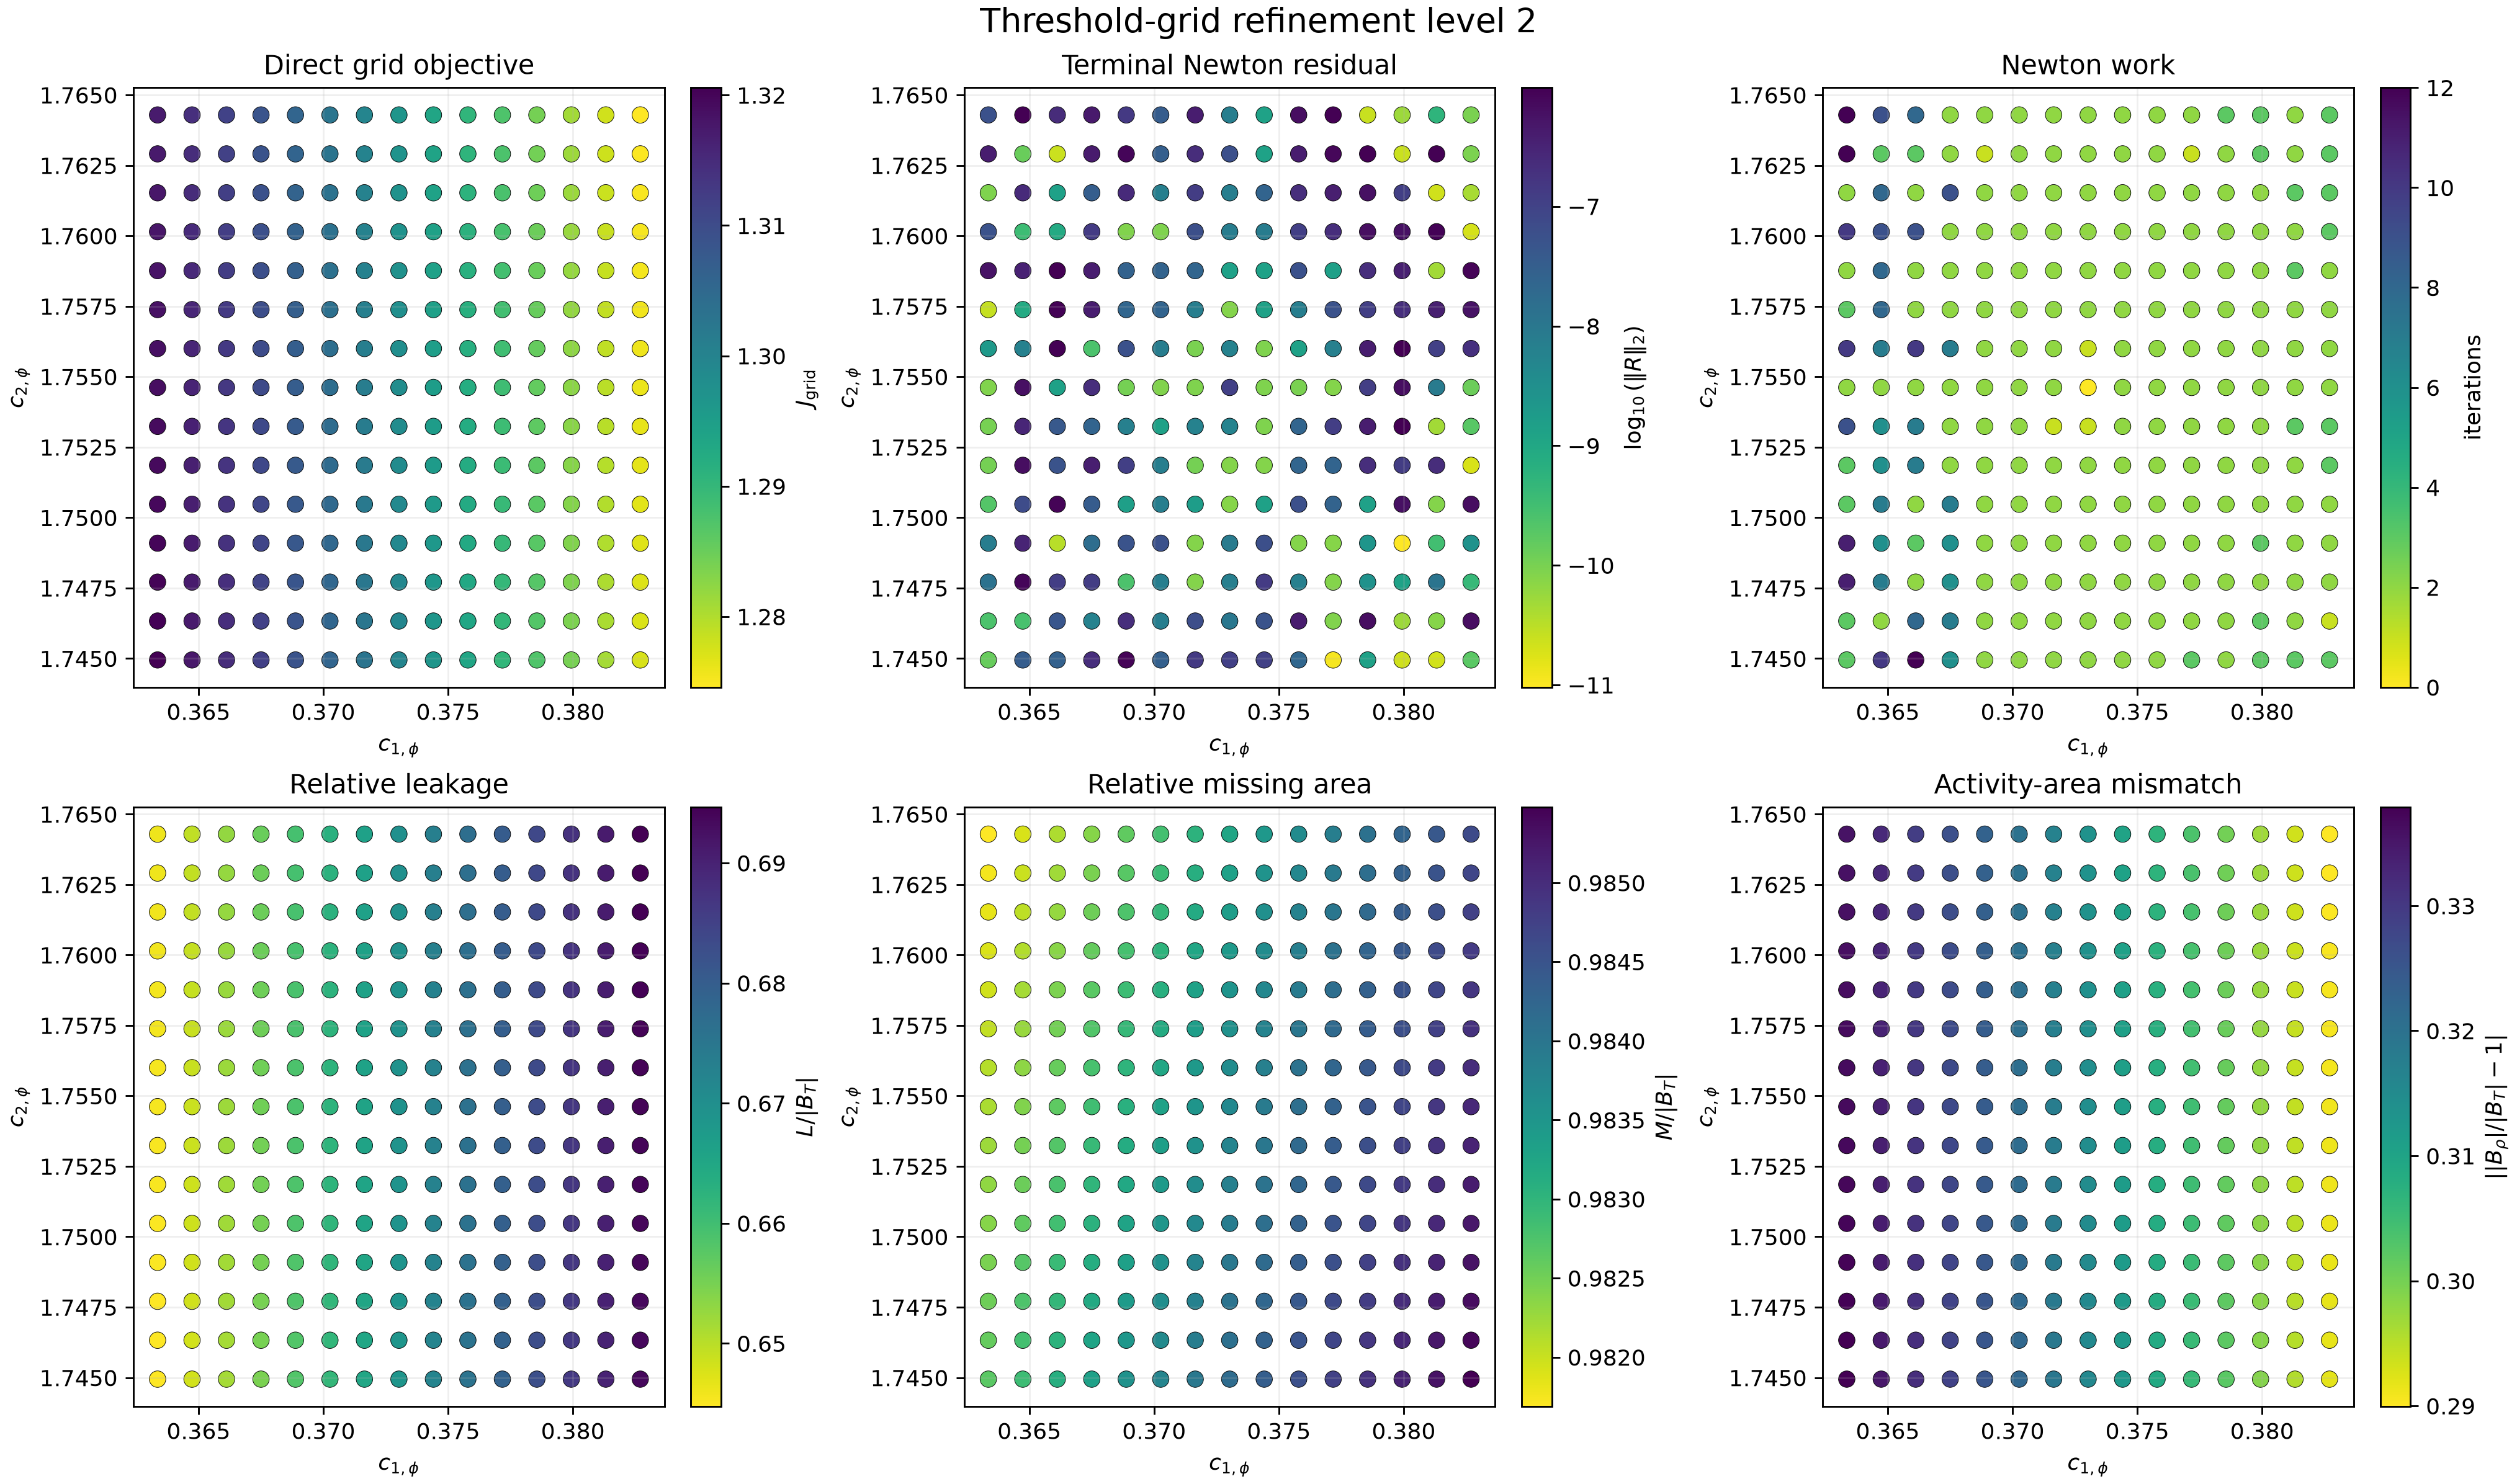
\includegraphics[width=0.97\linewidth]{figures/iter_0p6_0p7_torsion_cap_fine_grid_level_2.png}
\caption{Fine refinement diagnostics. The objective decreases toward the upper c1Phi and c2Phi corner, so this level supplies a robust PDE initializer but does not certify an interior threshold minimizer. Data status: actual; fine-grid boundary trend unresolved.}
\label{fig:iter-torsion-cap-grid-level-2}
\end{figure}
\end{landscape}

\begin{landscape}
\begin{figure}[tbp]
\centering
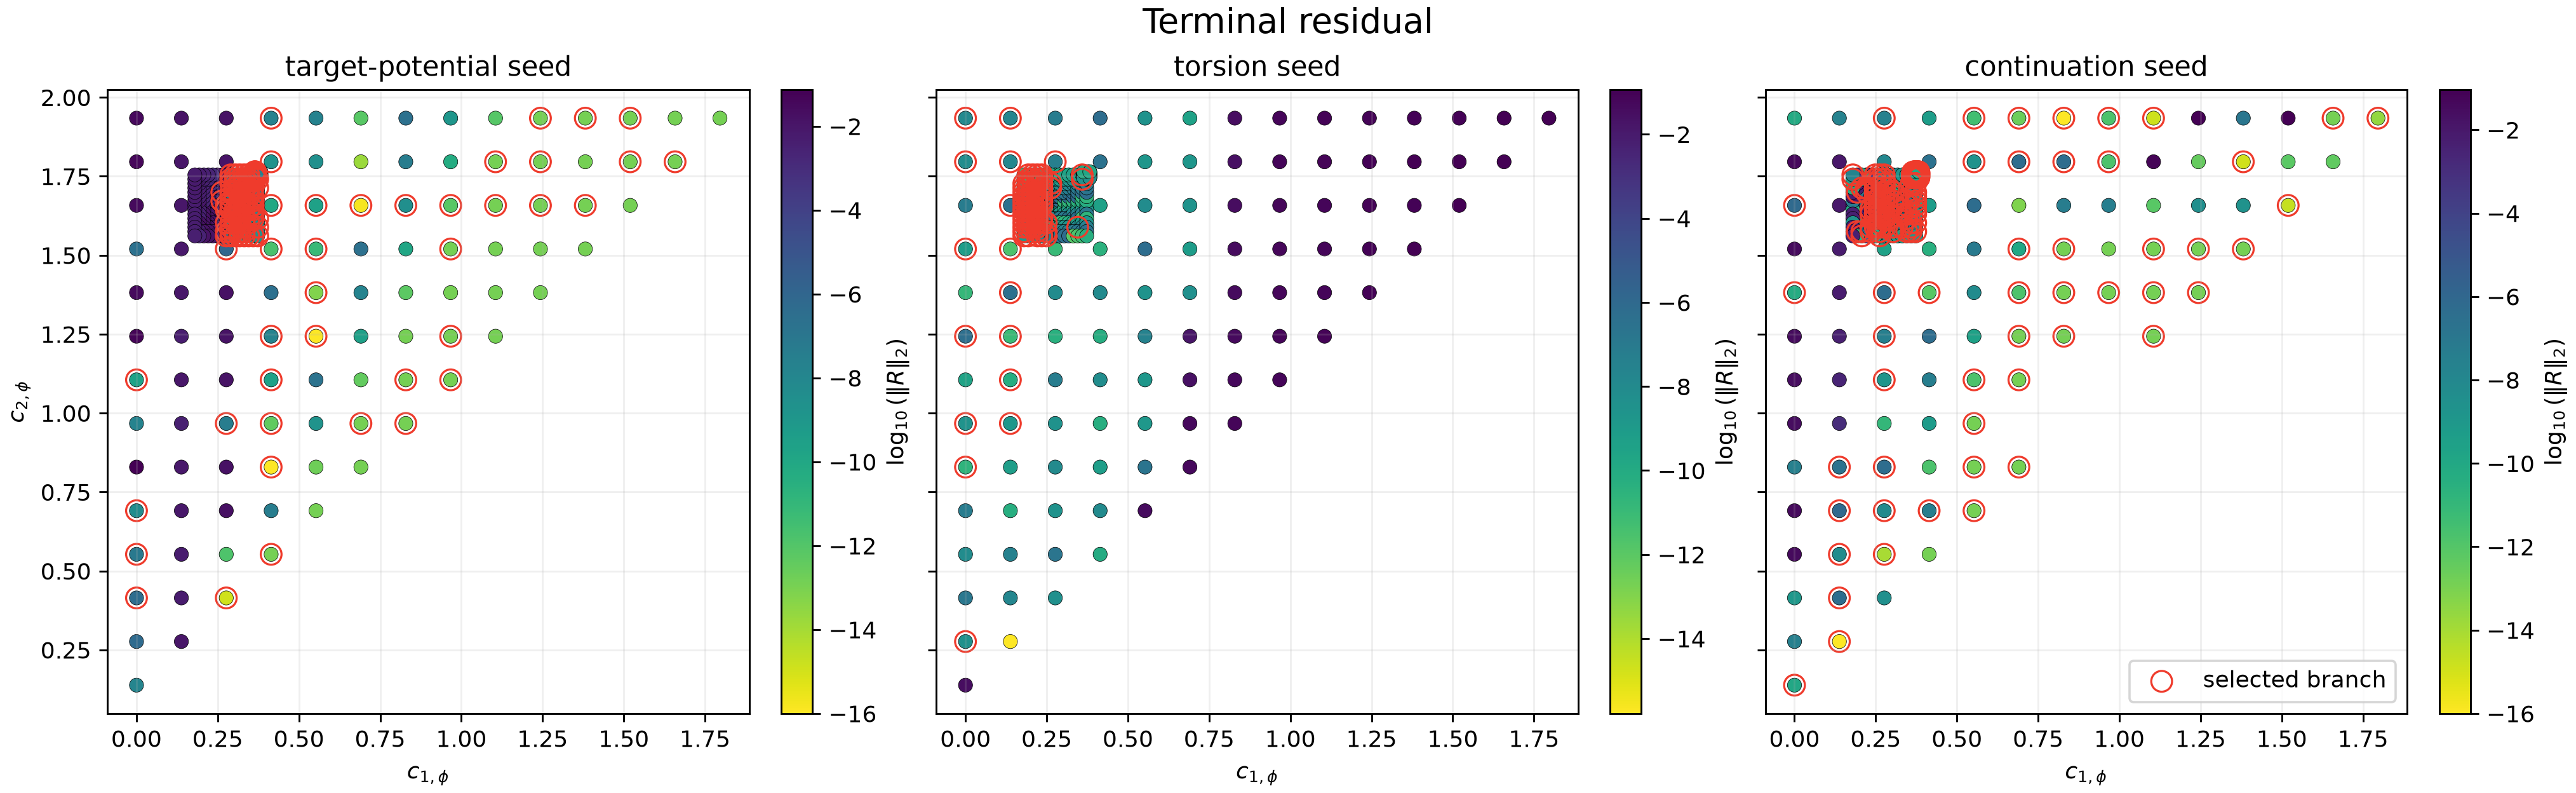
\includegraphics[width=0.97\linewidth]{figures/iter_0p6_0p7_torsion_cap_fine_branch_residuals.png}
\caption{Terminal Newton residual by seed family. Target-potential, torsion, and within-group continuation seeds are solved independently; red rings identify the branch selected for each threshold pair. Data status: actual; all 1660 branch trials retained.}
\label{fig:iter-torsion-cap-branch-residuals}
\end{figure}
\end{landscape}

\begin{landscape}
\begin{figure}[tbp]
\centering
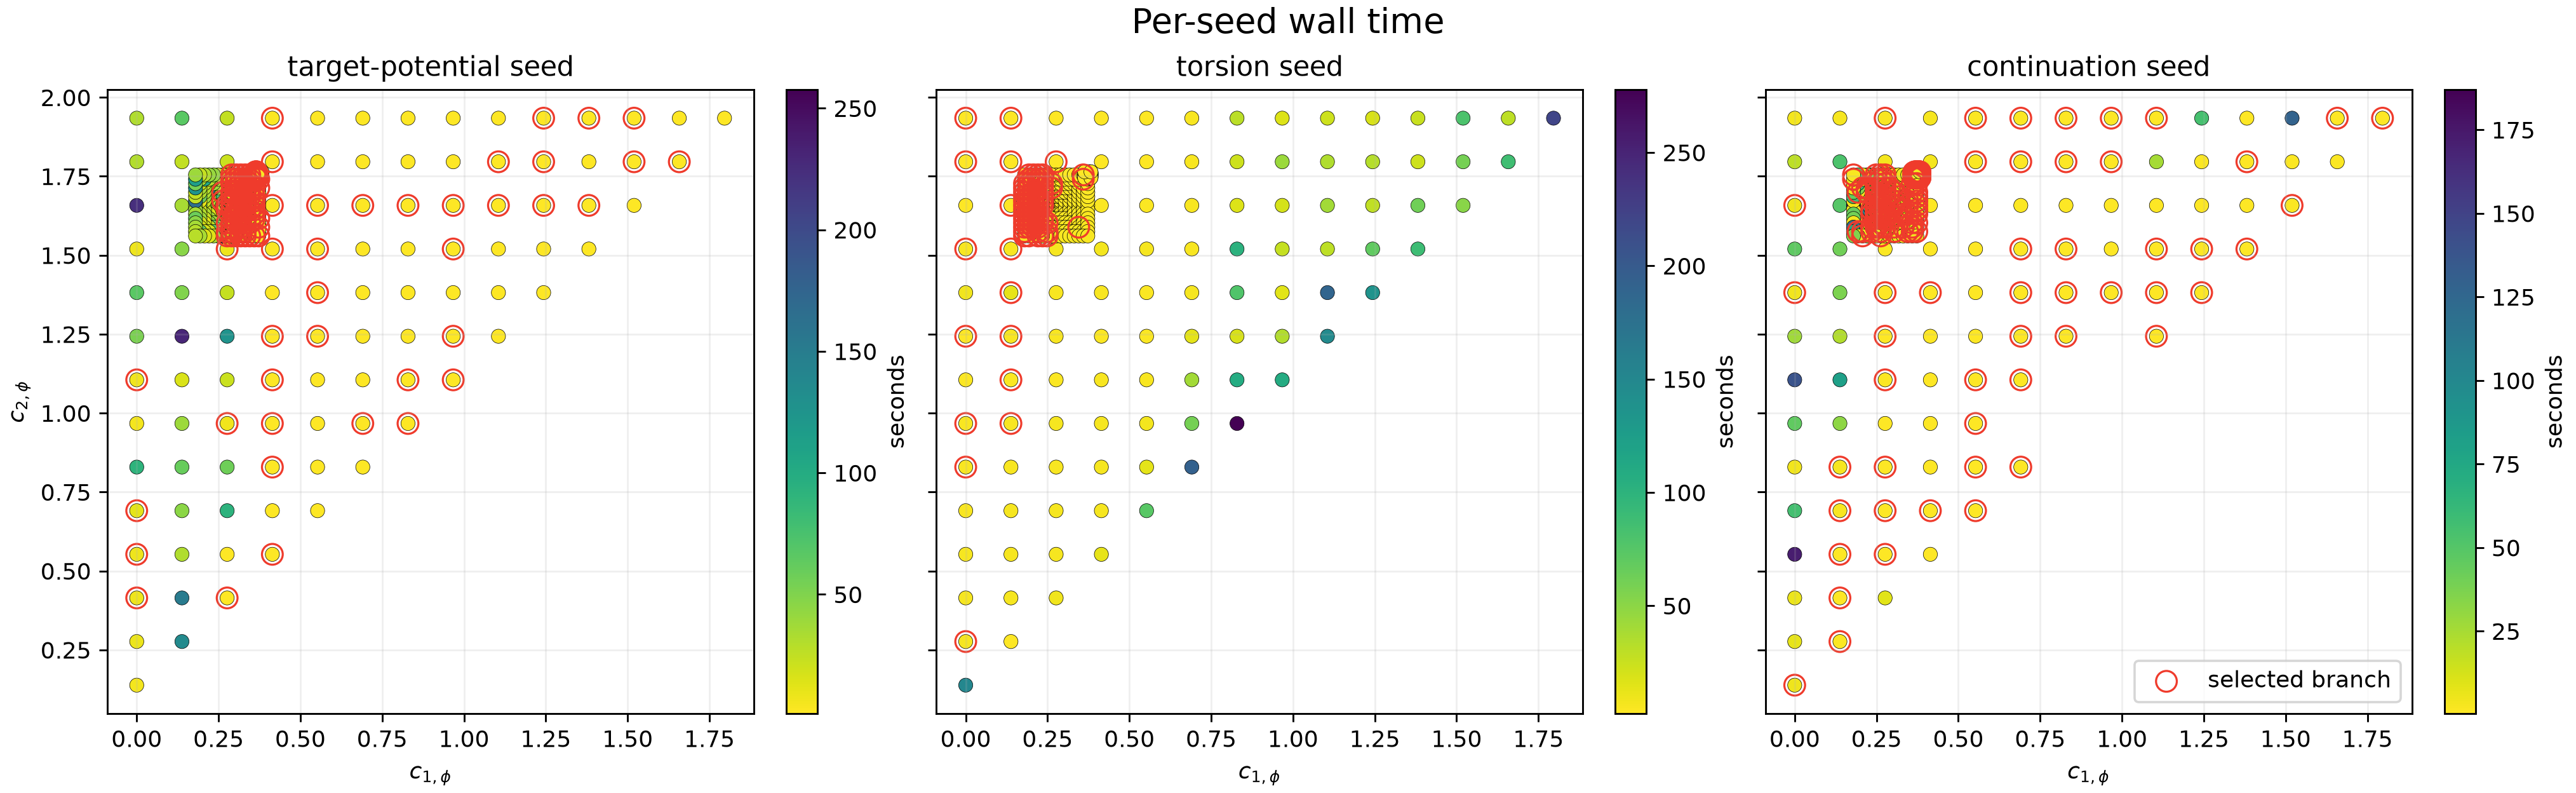
\includegraphics[width=0.97\linewidth]{figures/iter_0p6_0p7_torsion_cap_fine_branch_timing.png}
\caption{Per-seed Newton wall time across the expanded grid. Continuation has the smallest median cost (2.69 s), while isolated alternate branches produce the long tail retained in the robustness record. Data status: actual; five concurrent four-rank MUMPS groups.}
\label{fig:iter-torsion-cap-branch-timing}
\end{figure}
\end{landscape}

\begin{figure}[tbp]
\centering
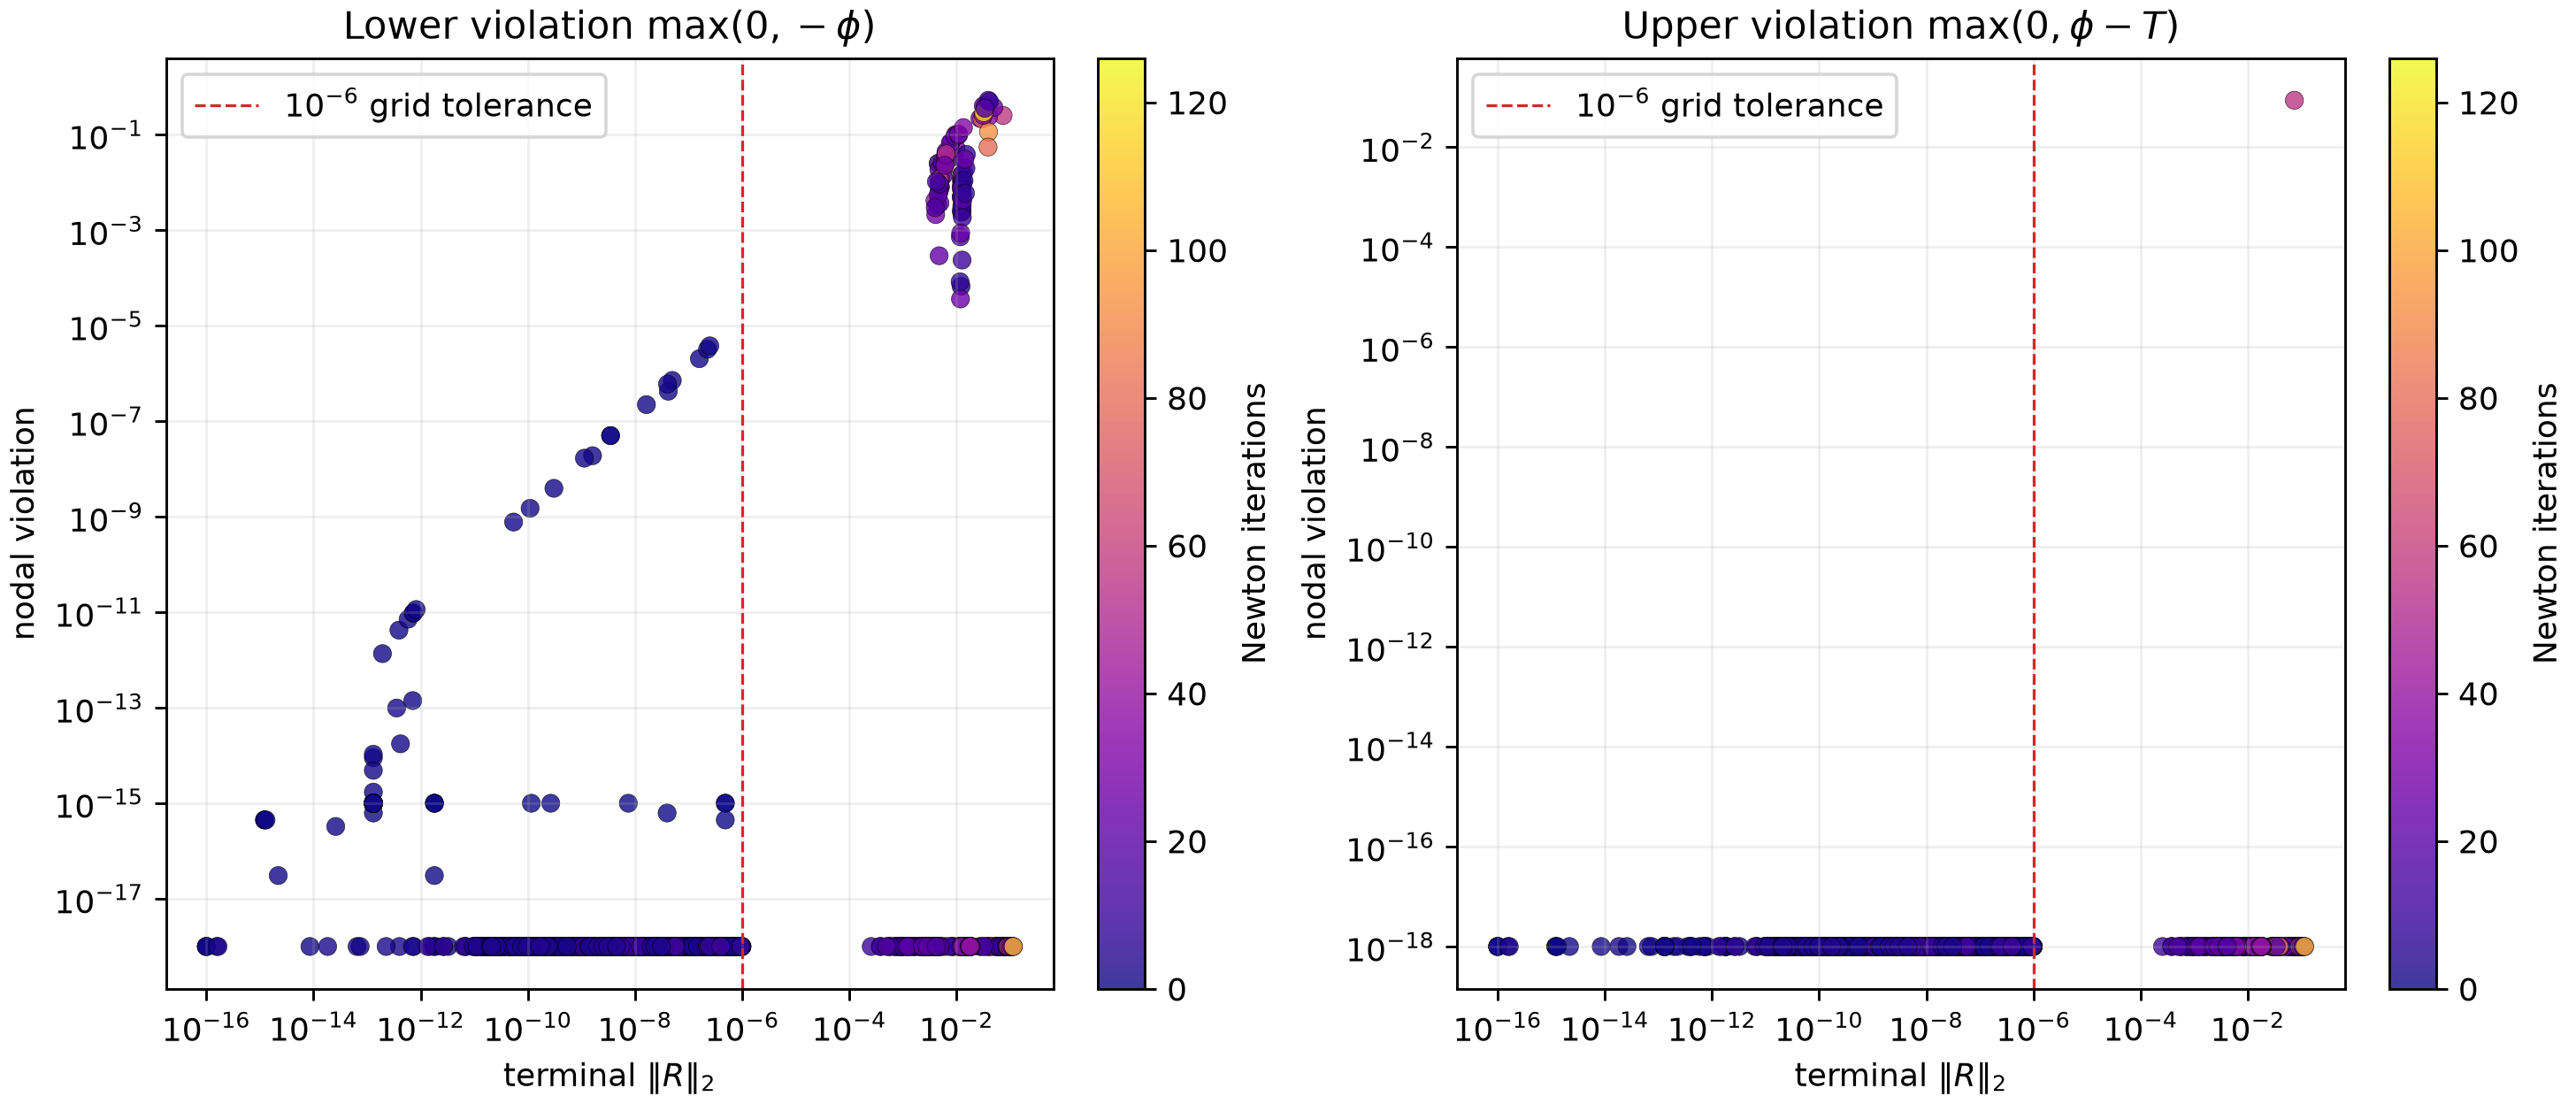
\includegraphics[width=0.88\linewidth]{figures/iter_0p6_0p7_torsion_cap_fine_maximum_principle.png}
\caption{Lower and upper nodal violations against terminal residual for every seed attempt. Candidate selection requires the effective bound check 0 <= phi <= T, with tolerance max(1e-8,10 times the grid residual tolerance). Data status: actual; discrete physical-bound audit.}
\label{fig:iter-torsion-cap-maximum-principle}
\end{figure}

\begin{landscape}
\begin{figure}[tbp]
\centering
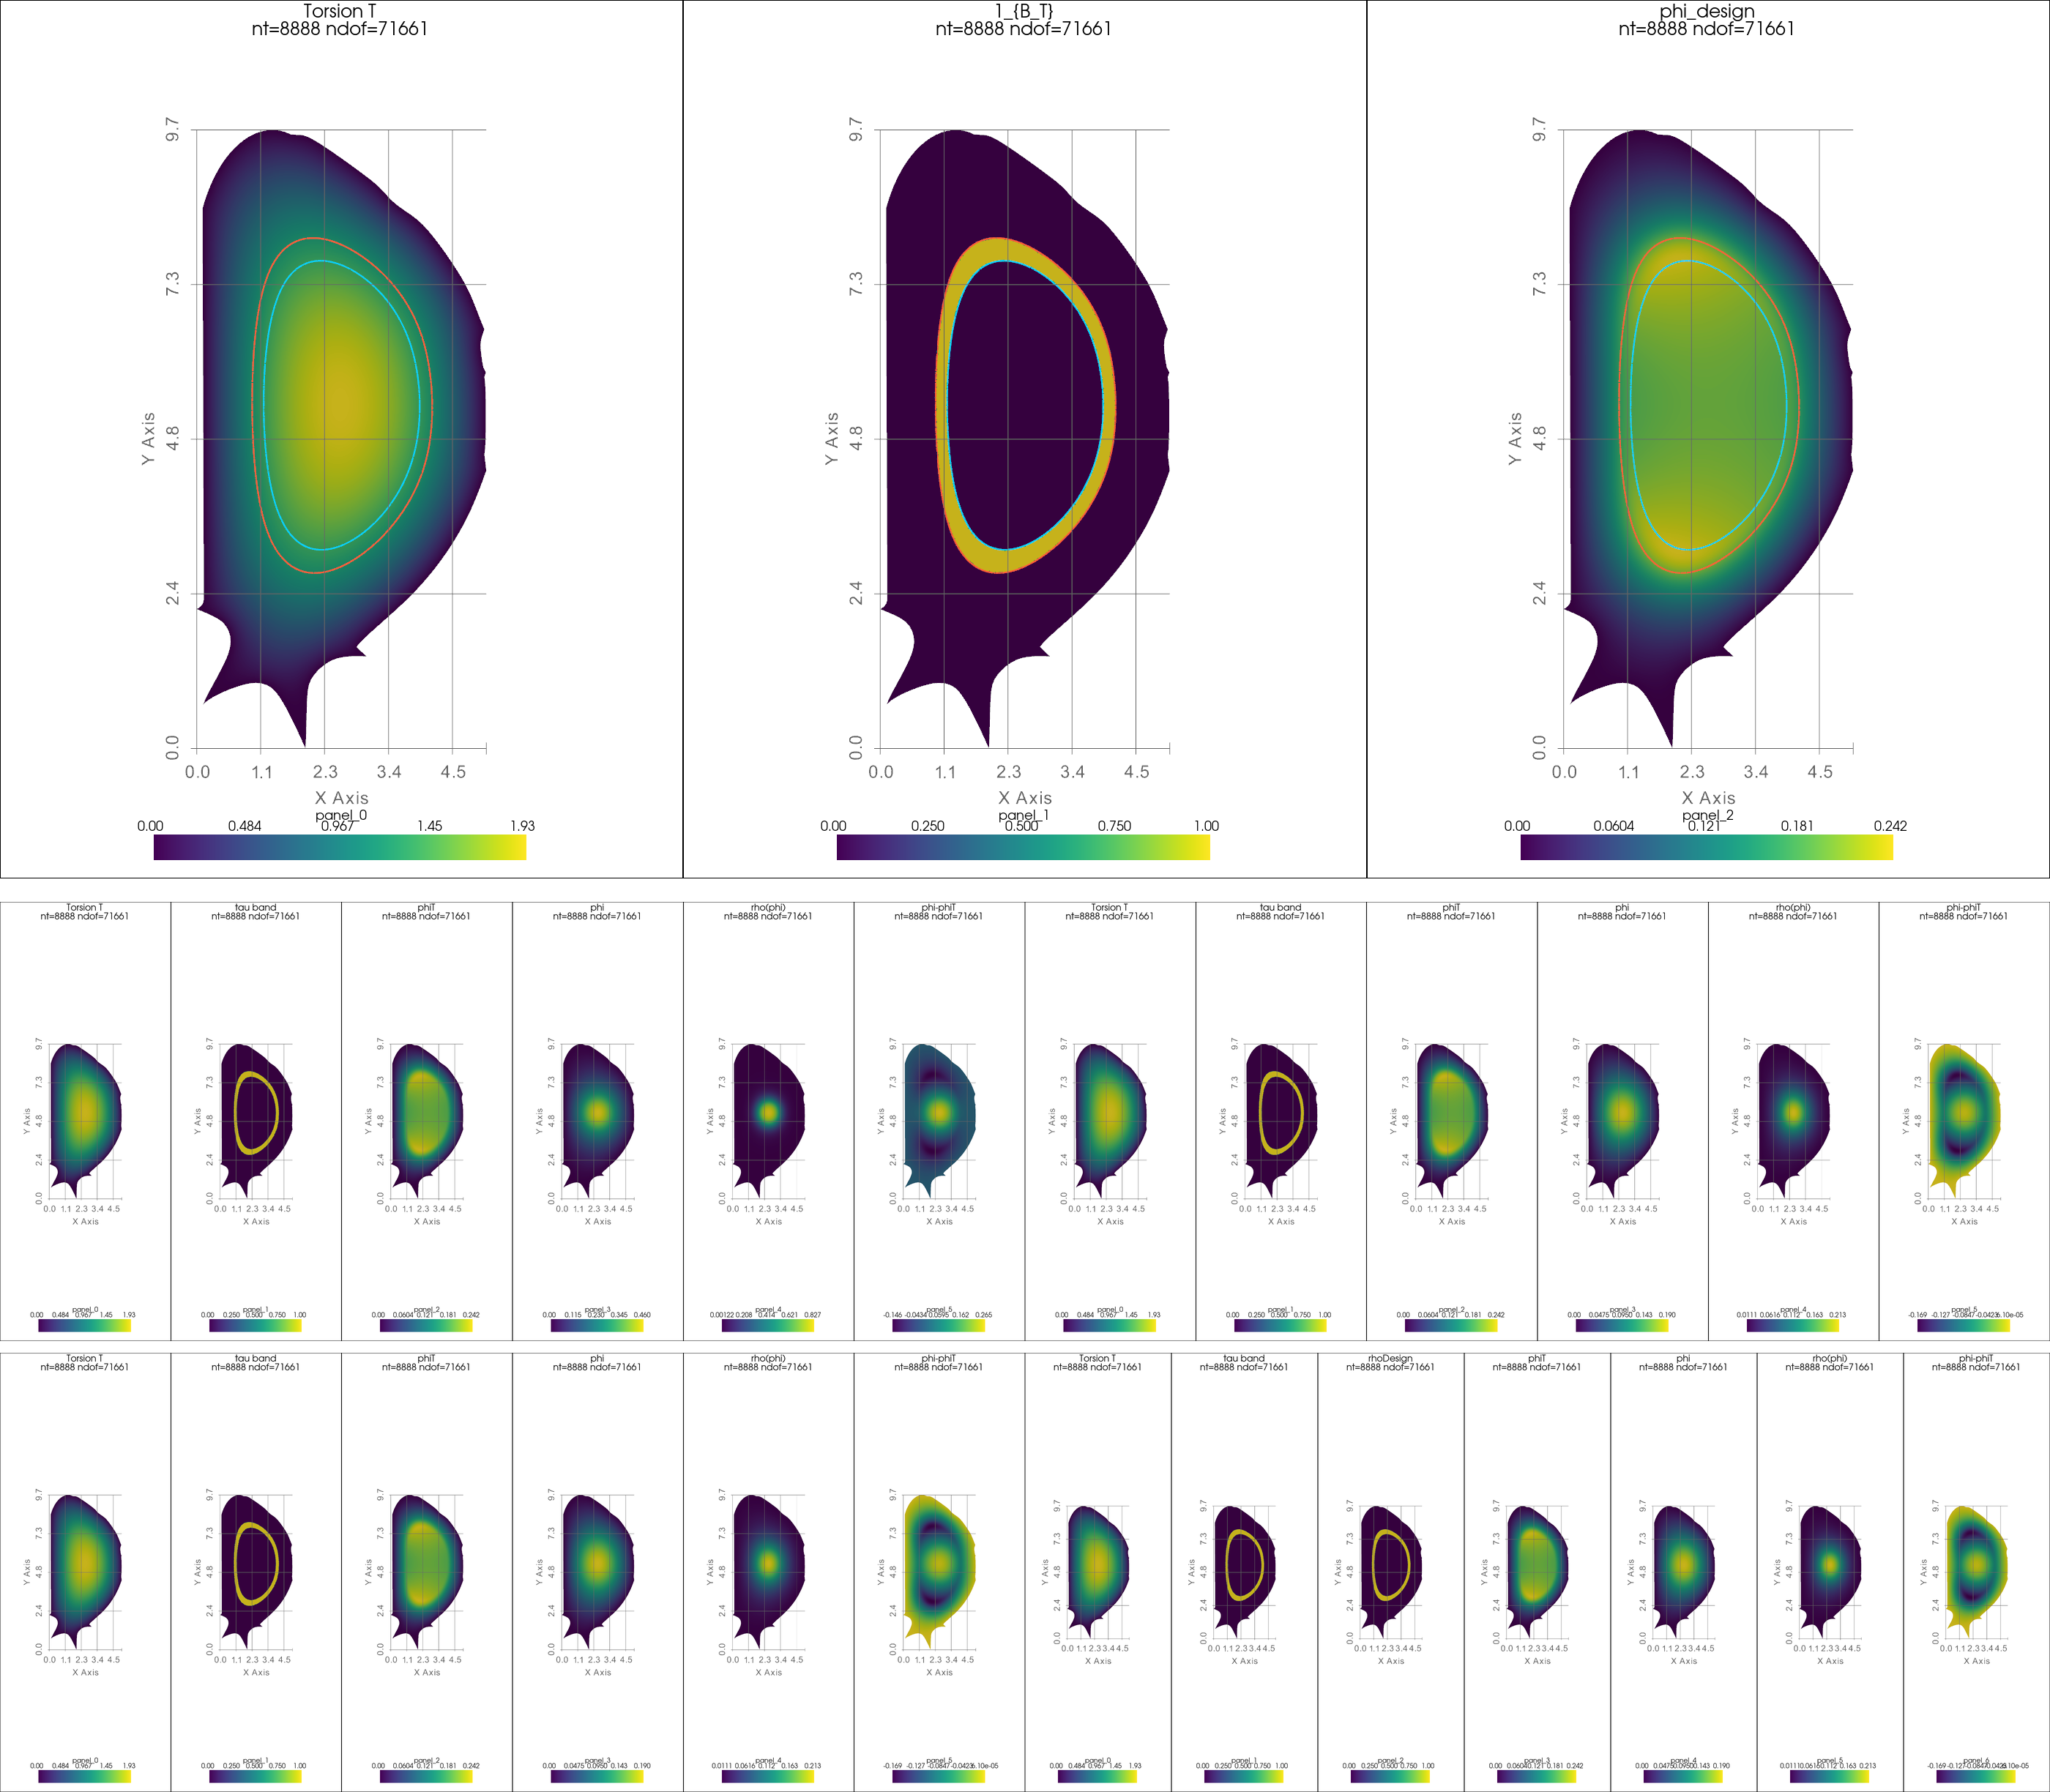
\includegraphics[width=0.70\linewidth]{figures/iter_0p6_0p7_torsion_cap_fine_storyboard.png}
\caption{ITER design fields shown once above selected early, middle, late, and final threshold states. Rank zero gathered all 8888 cells and 71661 P4 degrees of freedom; mesh edges are suppressed. The final residual is 9.57e-15, but the certified area is zero. Data status: actual; PDE-converged, geometrically unsuccessful plateau.}
\label{fig:iter-torsion-cap-storyboard}
\end{figure}
\end{landscape}

\clearpage

\begin{figure}[tbp]
\centering
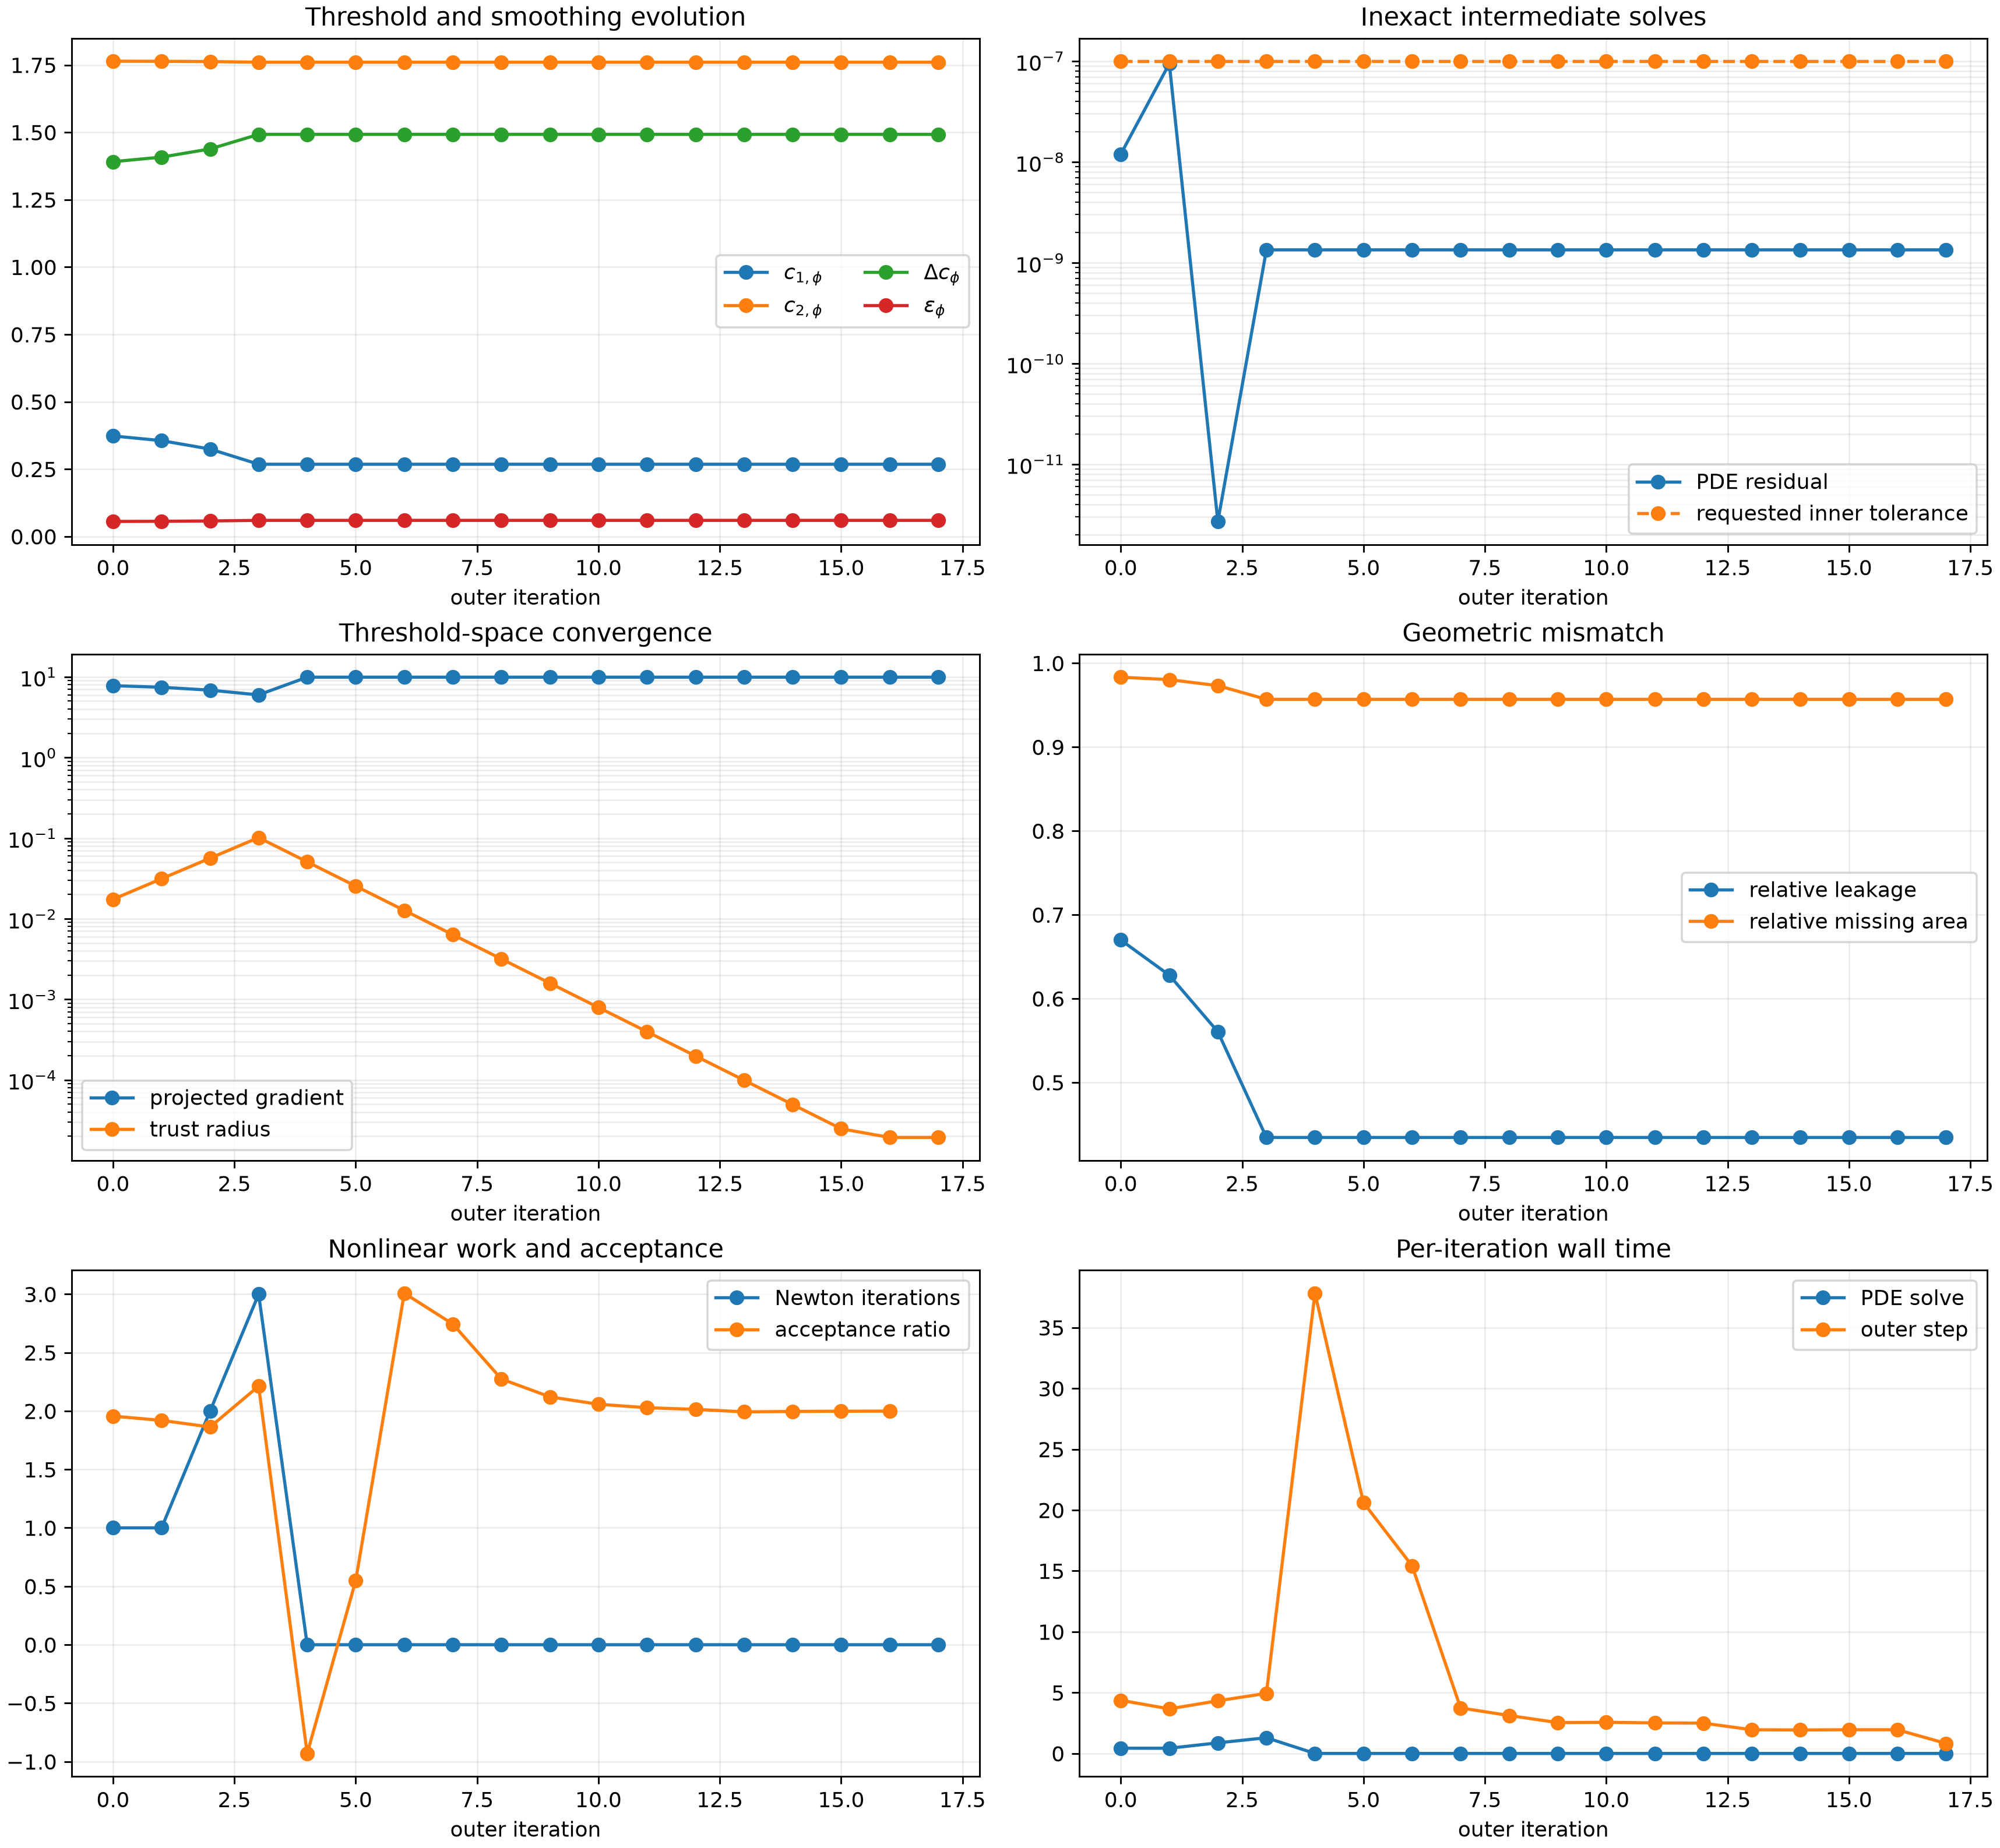
\includegraphics[width=0.86\linewidth]{figures/iter_0p6_0p7_torsion_cap_fine_optimization_trace.png}
\caption{Reduced-optimization trace separating threshold motion, inexact PDE residual, projected gradient, geometric discrepancies, nonlinear work, acceptance ratio, and time. Four steps are accepted before fourteen rejections drive the trust radius to the step floor. Data status: actual; trust-limited threshold plateau.}
\label{fig:iter-torsion-cap-optimization-trace}
\end{figure}

\begin{landscape}
\begin{figure}[tbp]
\centering
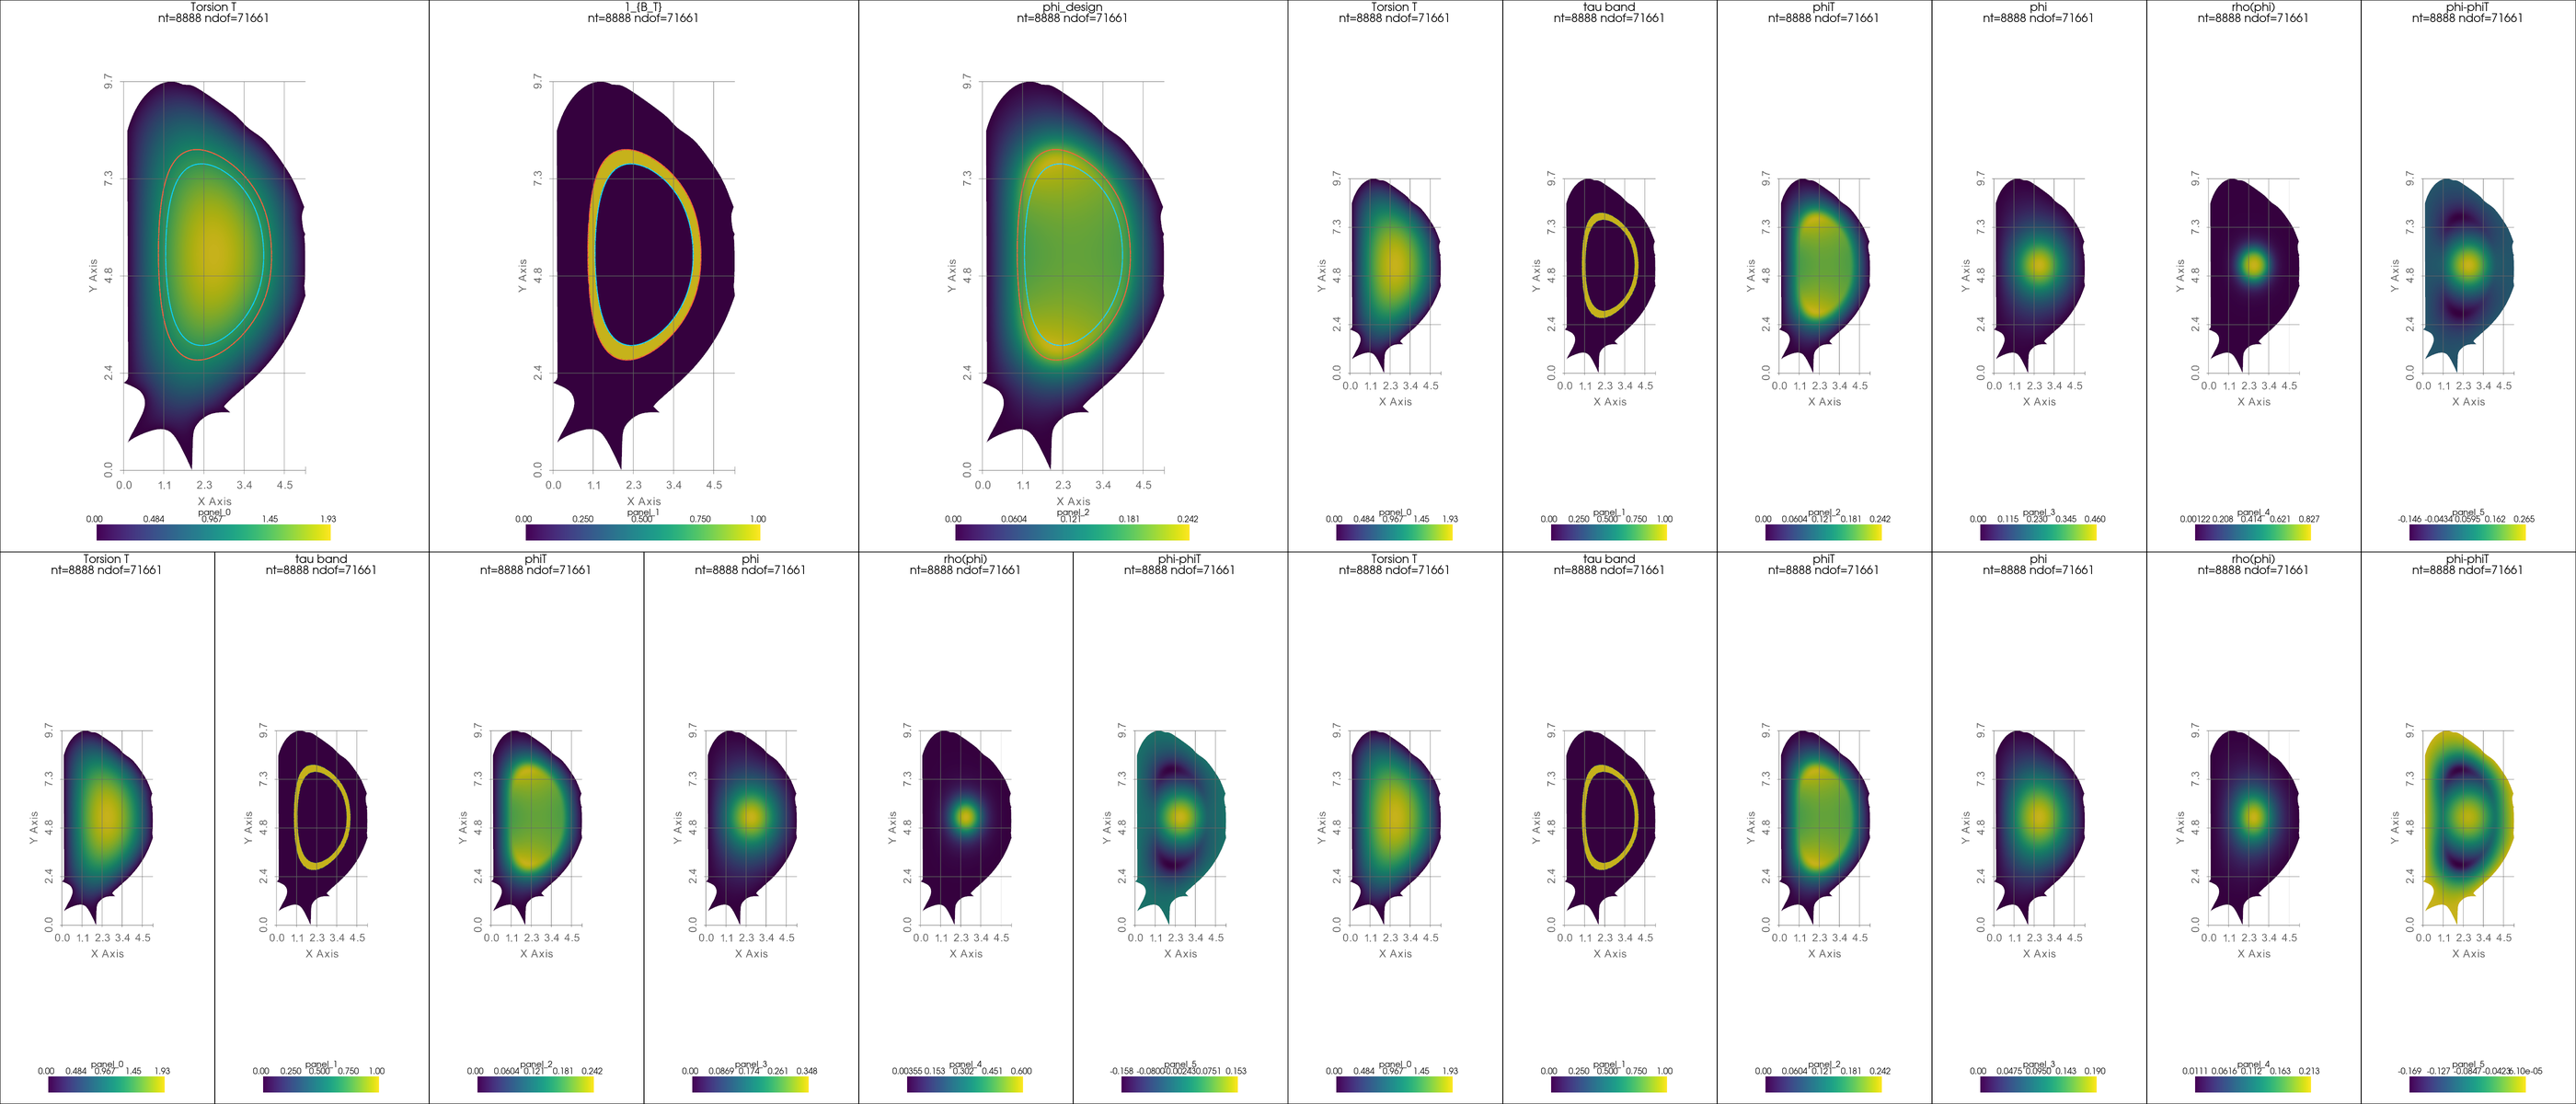
\includegraphics[width=0.97\linewidth]{figures/iter_0p6_0p7_torsion_cap_fine_frames_contact_01.png}
\caption{First contact sheet from the complete high-resolution frame archive: design, the grid-selected state, and the first accepted threshold updates. The source PNGs remain available at 2800 by 1200 pixels. Data status: actual; native frames 0 through 2.}
\label{fig:iter-torsion-cap-contact-1}
\end{figure}
\end{landscape}

\begin{landscape}
\begin{figure}[tbp]
\centering
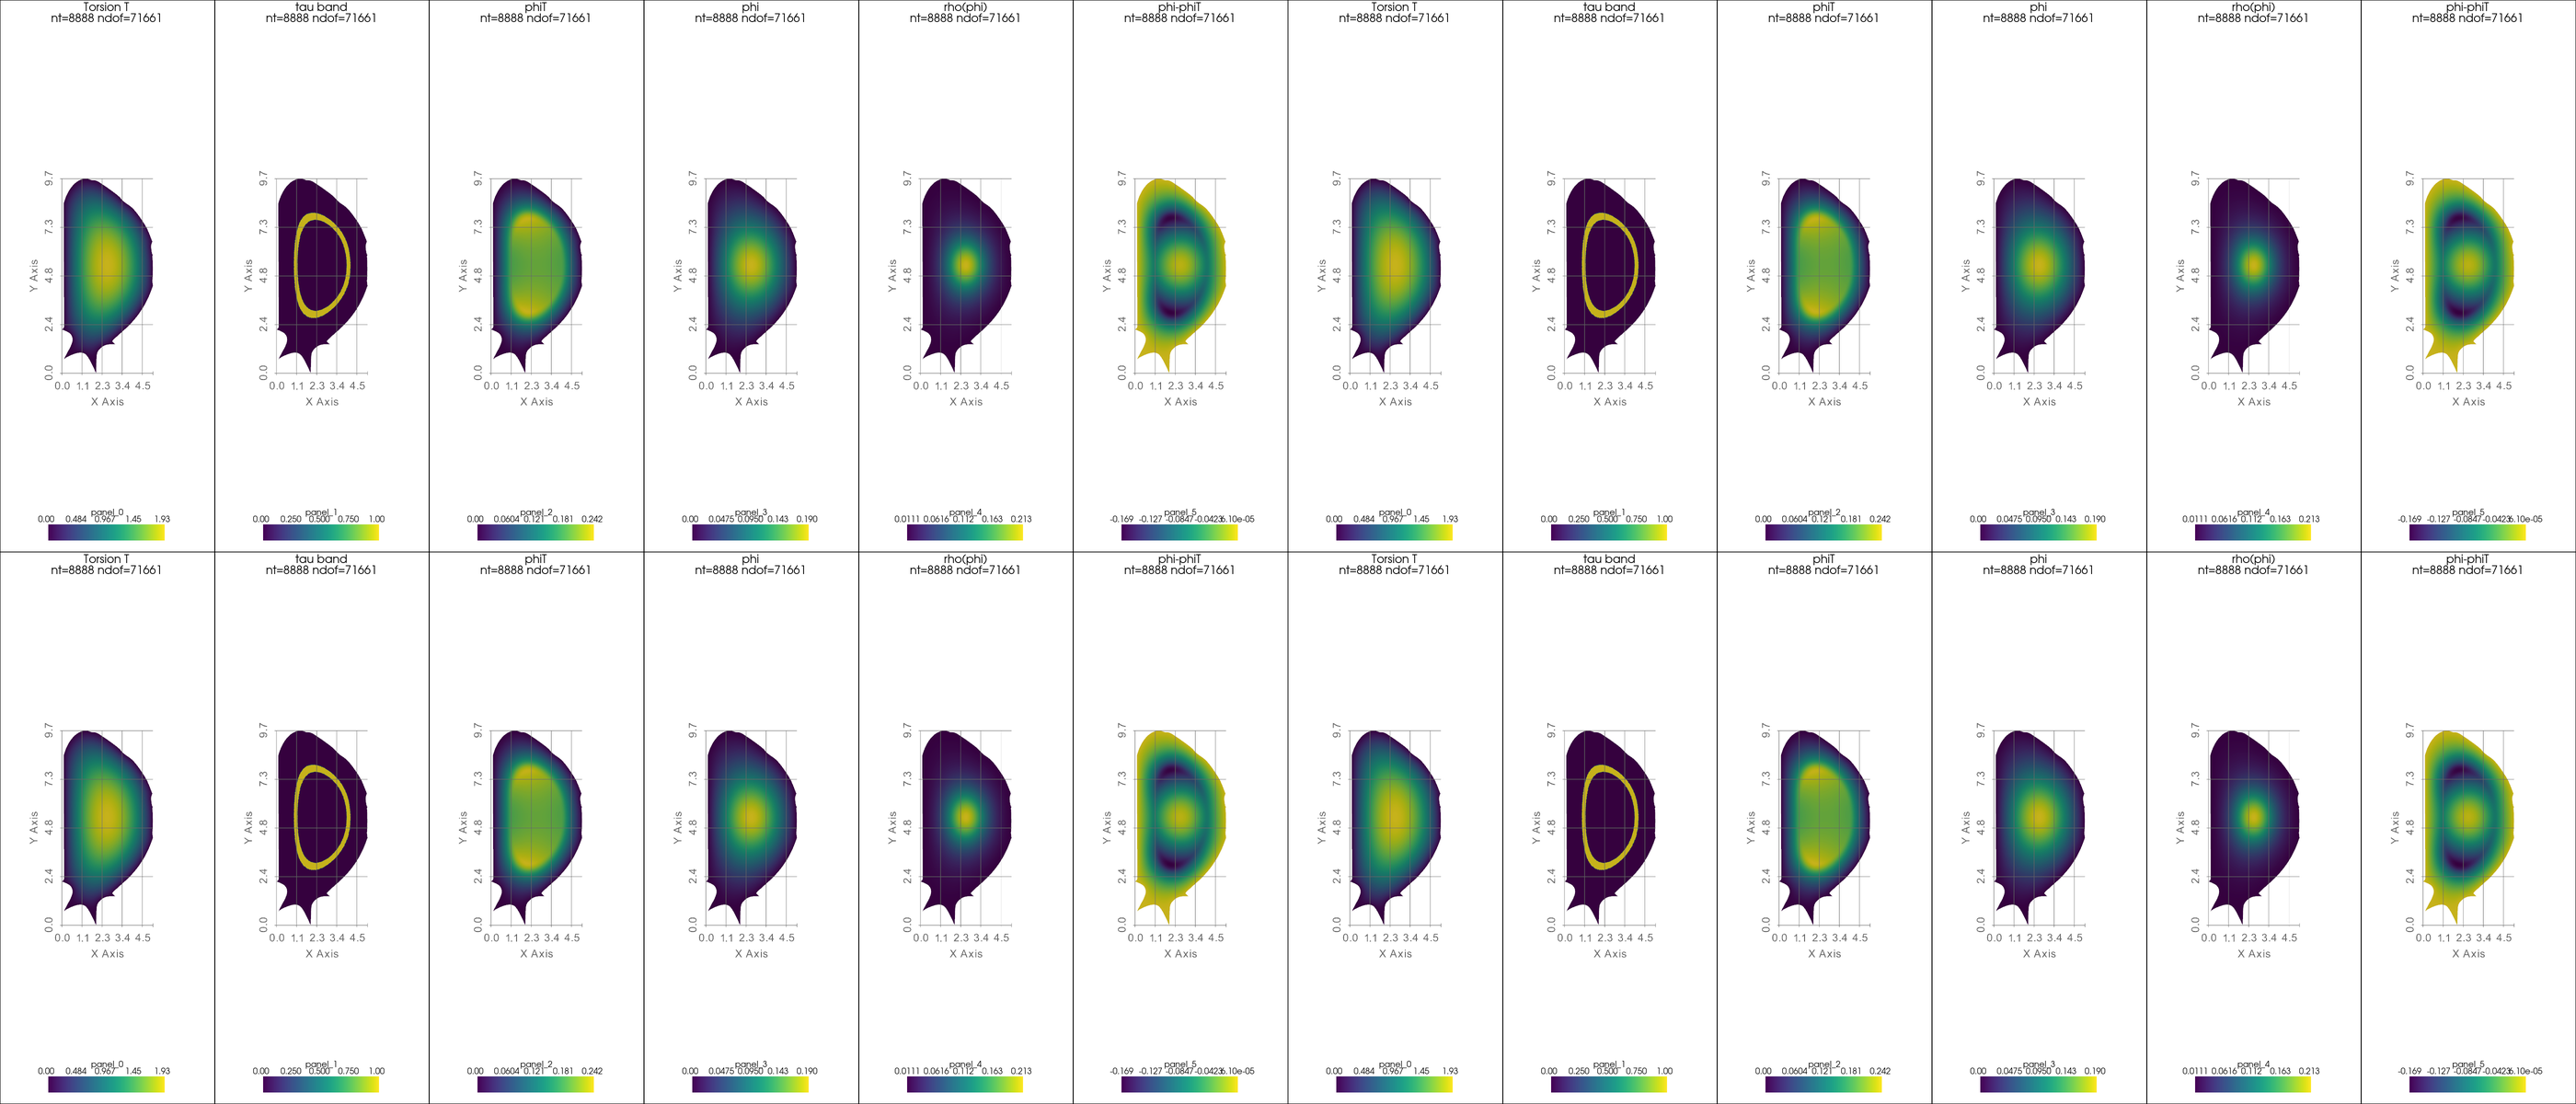
\includegraphics[width=0.97\linewidth]{figures/iter_0p6_0p7_torsion_cap_fine_frames_contact_02.png}
\caption{Second contact sheet from the ITER frame archive, showing the onset of repeated rejected threshold steps while the PDE state remains converged. Data status: actual; rejected-step plateau sequence.}
\label{fig:iter-torsion-cap-contact-2}
\end{figure}
\end{landscape}

\begin{landscape}
\begin{figure}[tbp]
\centering
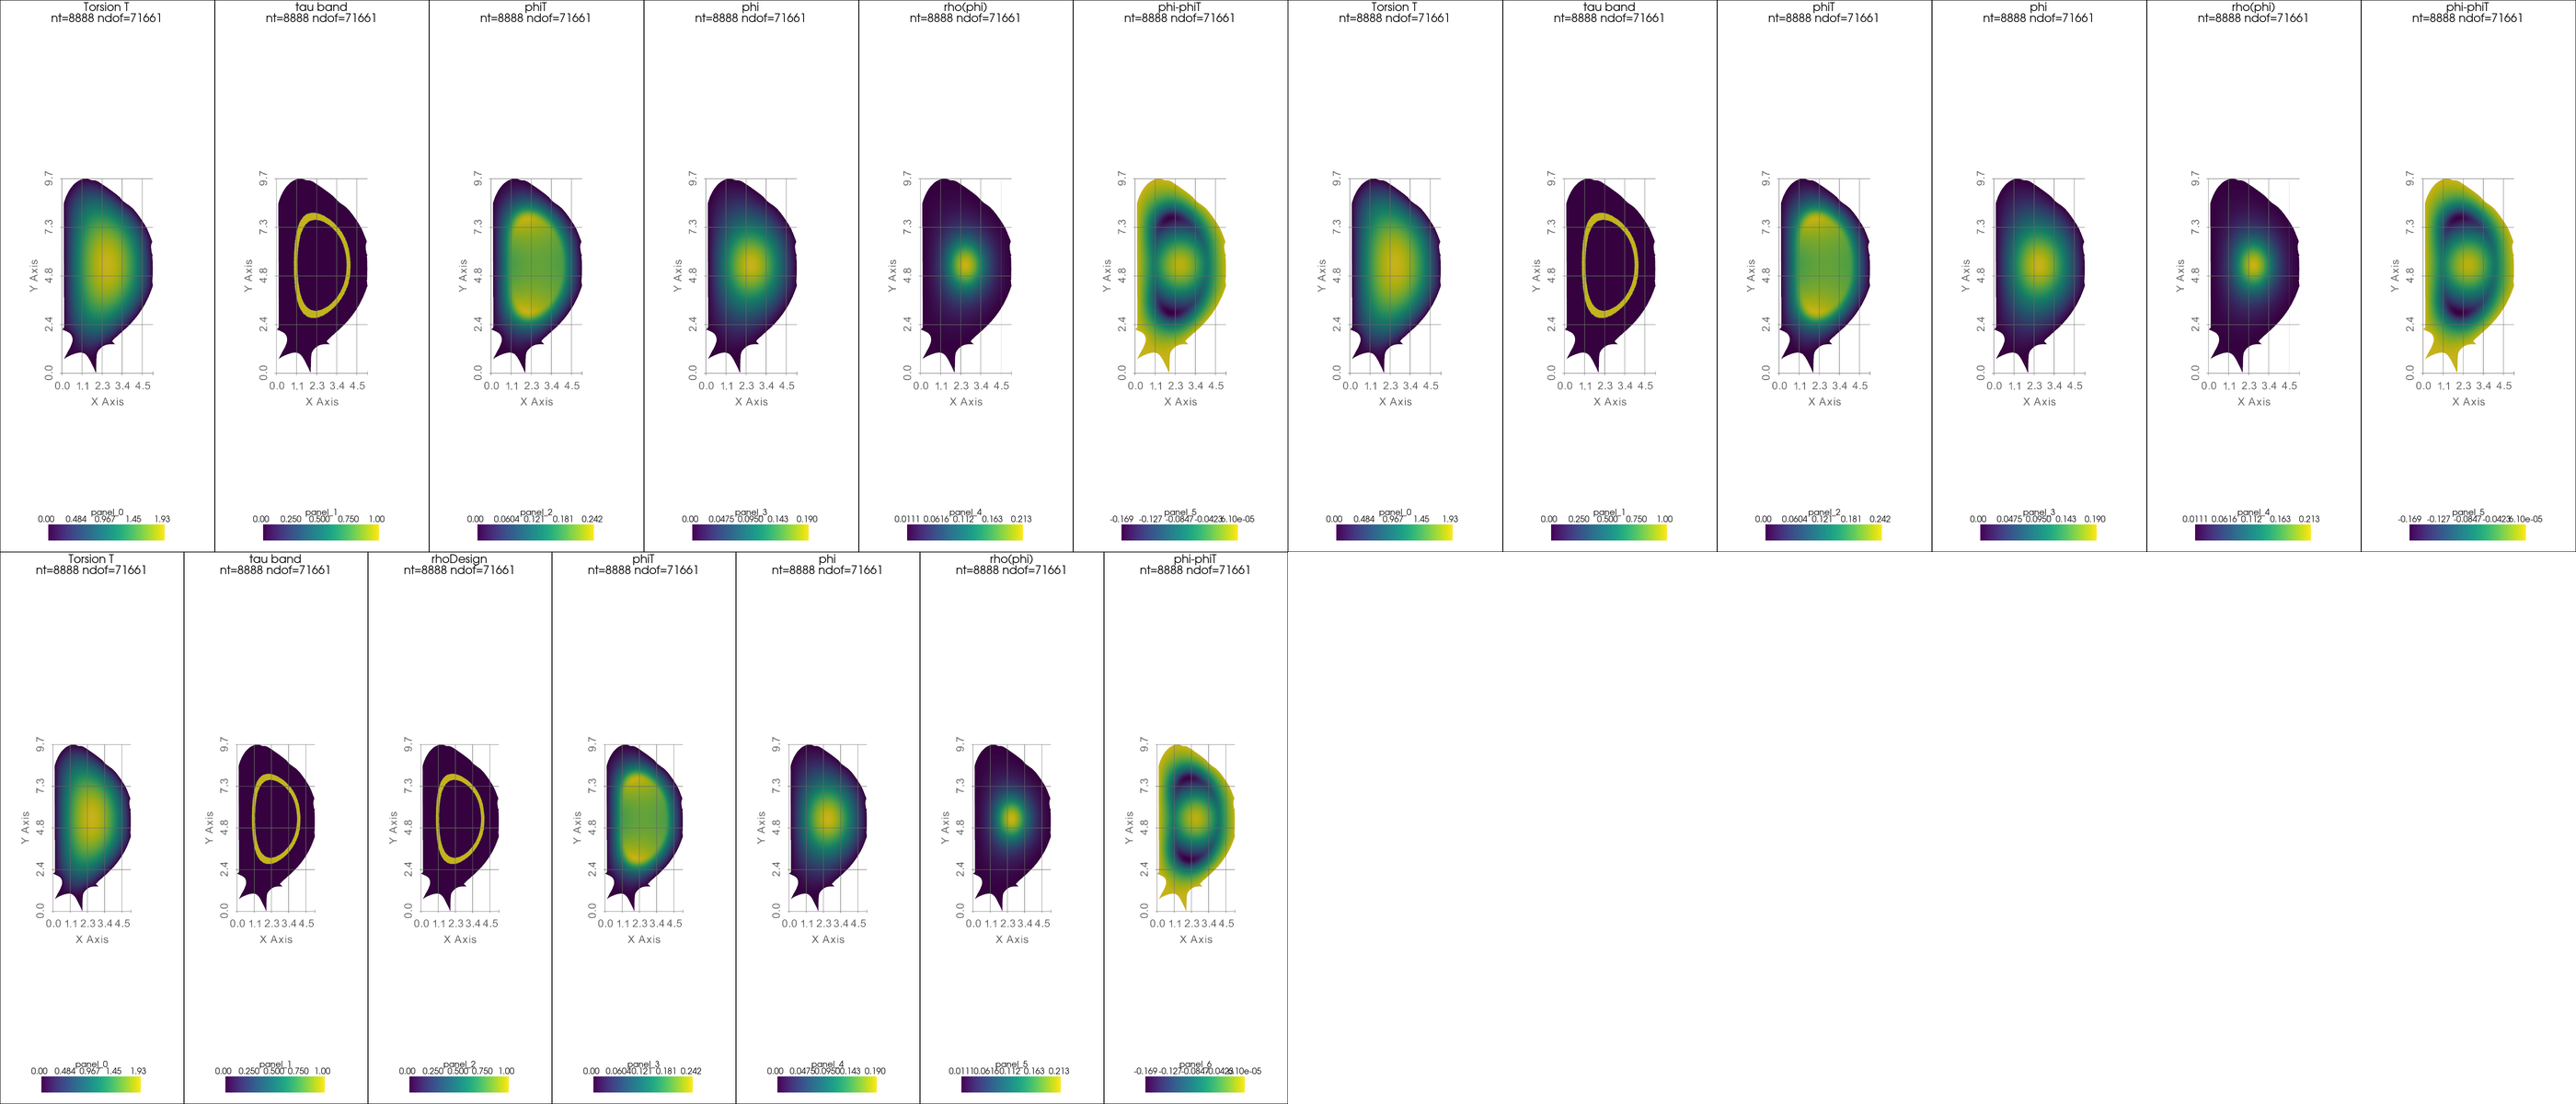
\includegraphics[width=0.97\linewidth]{figures/iter_0p6_0p7_torsion_cap_fine_frames_contact_03.png}
\caption{Late rejected-step states and the exact final MUMPS projection. These failure frames are retained rather than omitted from the qualitative convergence record. Data status: actual; late plateau and final projection.}
\label{fig:iter-torsion-cap-contact-3}
\end{figure}
\end{landscape}

\subsection{Corrected active-contour brute-force diagnostic for ITER}
\label{sec:iter-corrected-bruteforce}

We repeated the difficult ITER $[0.60,0.70]$ experiment after correcting the
candidate objective and the reduced-step acceptance audit.  This deliberately
inexpensive control uses $2{,}281$ triangles, $18{,}527$ global P4 degrees of
freedom, $h_{\max}=0.245148$, a discontinuous torsion target, and
\(\varepsilon_\phi/\Delta c_\phi=0.02\).  Twelve MPI ranks were split into
twelve independent one-rank MUMPS candidate groups, in agreement with the
measured rank policy below \(20{,}000\) degrees of freedom.  Two grid levels
evaluated 104 distinct threshold pairs and 299 independently seeded Newton
branches at residual tolerance \(10^{-6}\).  Of these pairs, 101 had a
residual-qualified branch.  Every pair, including partial and failed solves,
has a full-field PNG in
\texttt{grid\_search/candidate\_pairs/stage\_NNN}; the run validator rejects a
completed search if any of these PNGs is absent.

The corrected candidate functional is
\[
 {\cal J}_{\rm grid}
 = L_{\rm rel}+M_{\rm rel}
   +\left|A_{\rm active}/A_{\rm target}-1\right|.
\]
Selection additionally requires \(0\leq\phi\leq T\) and both threshold
contours to be active.  These conditions prevent cancellation between
leakage and missing area and prevent selecting thresholds that lie outside
the attained potential range.  The selected pair was
\((c_{1,\phi},c_{2,\phi})=(0.0700,0.0800)\), with residual
\(3.99\times10^{-7}\), \(L_{\rm rel}=0.80772\),
\(M_{\rm rel}=0.99672\), and
\(A_{\rm active}/A_{\rm target}=0.81100\).  Thus, the expanded search did not
solve the geometric problem: it found a valid nonlinear equilibrium on the
wrong spatial branch.

\begin{landscape}
\begin{figure}[tbp]
\centering
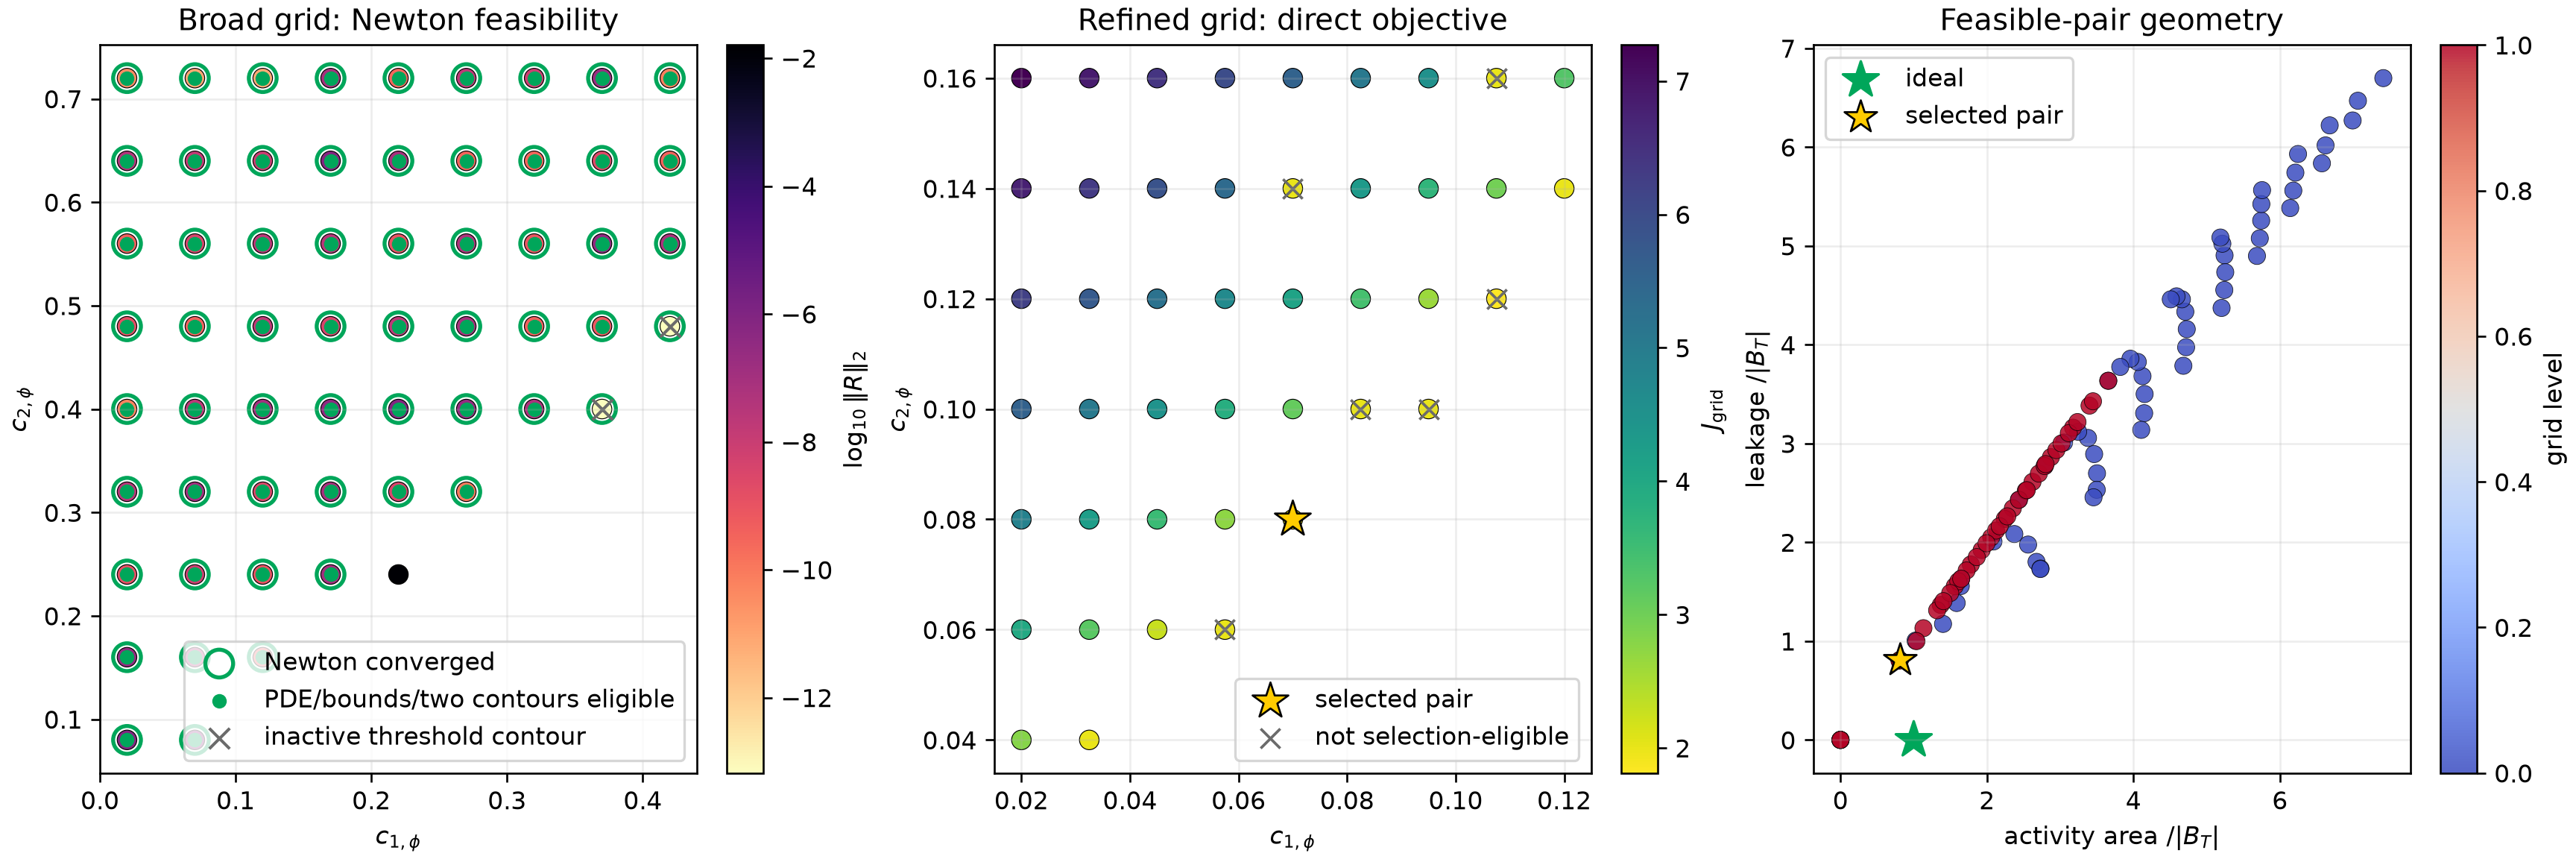
\includegraphics[width=0.97\linewidth]{figures/iter_0p6_0p7_bruteforce_active_eps002_lowdof_grid_search.png}
\caption{Corrected MPI-split threshold search for ITER $[0.60,0.70]$.  Marker shape separates residual-qualified, partial, and failed pairs; rings distinguish candidates with two active contours and candidates eligible for selection.  The star is the selected pair.  All unsuccessful candidates remain in the plot and in the per-pair PNG archive.  Data status: actual; 104 pairs and 299 Newton branches.}
\label{fig:iter-active-grid-search}
\end{figure}
\end{landscape}

\begin{landscape}
\begin{figure}[tbp]
\centering
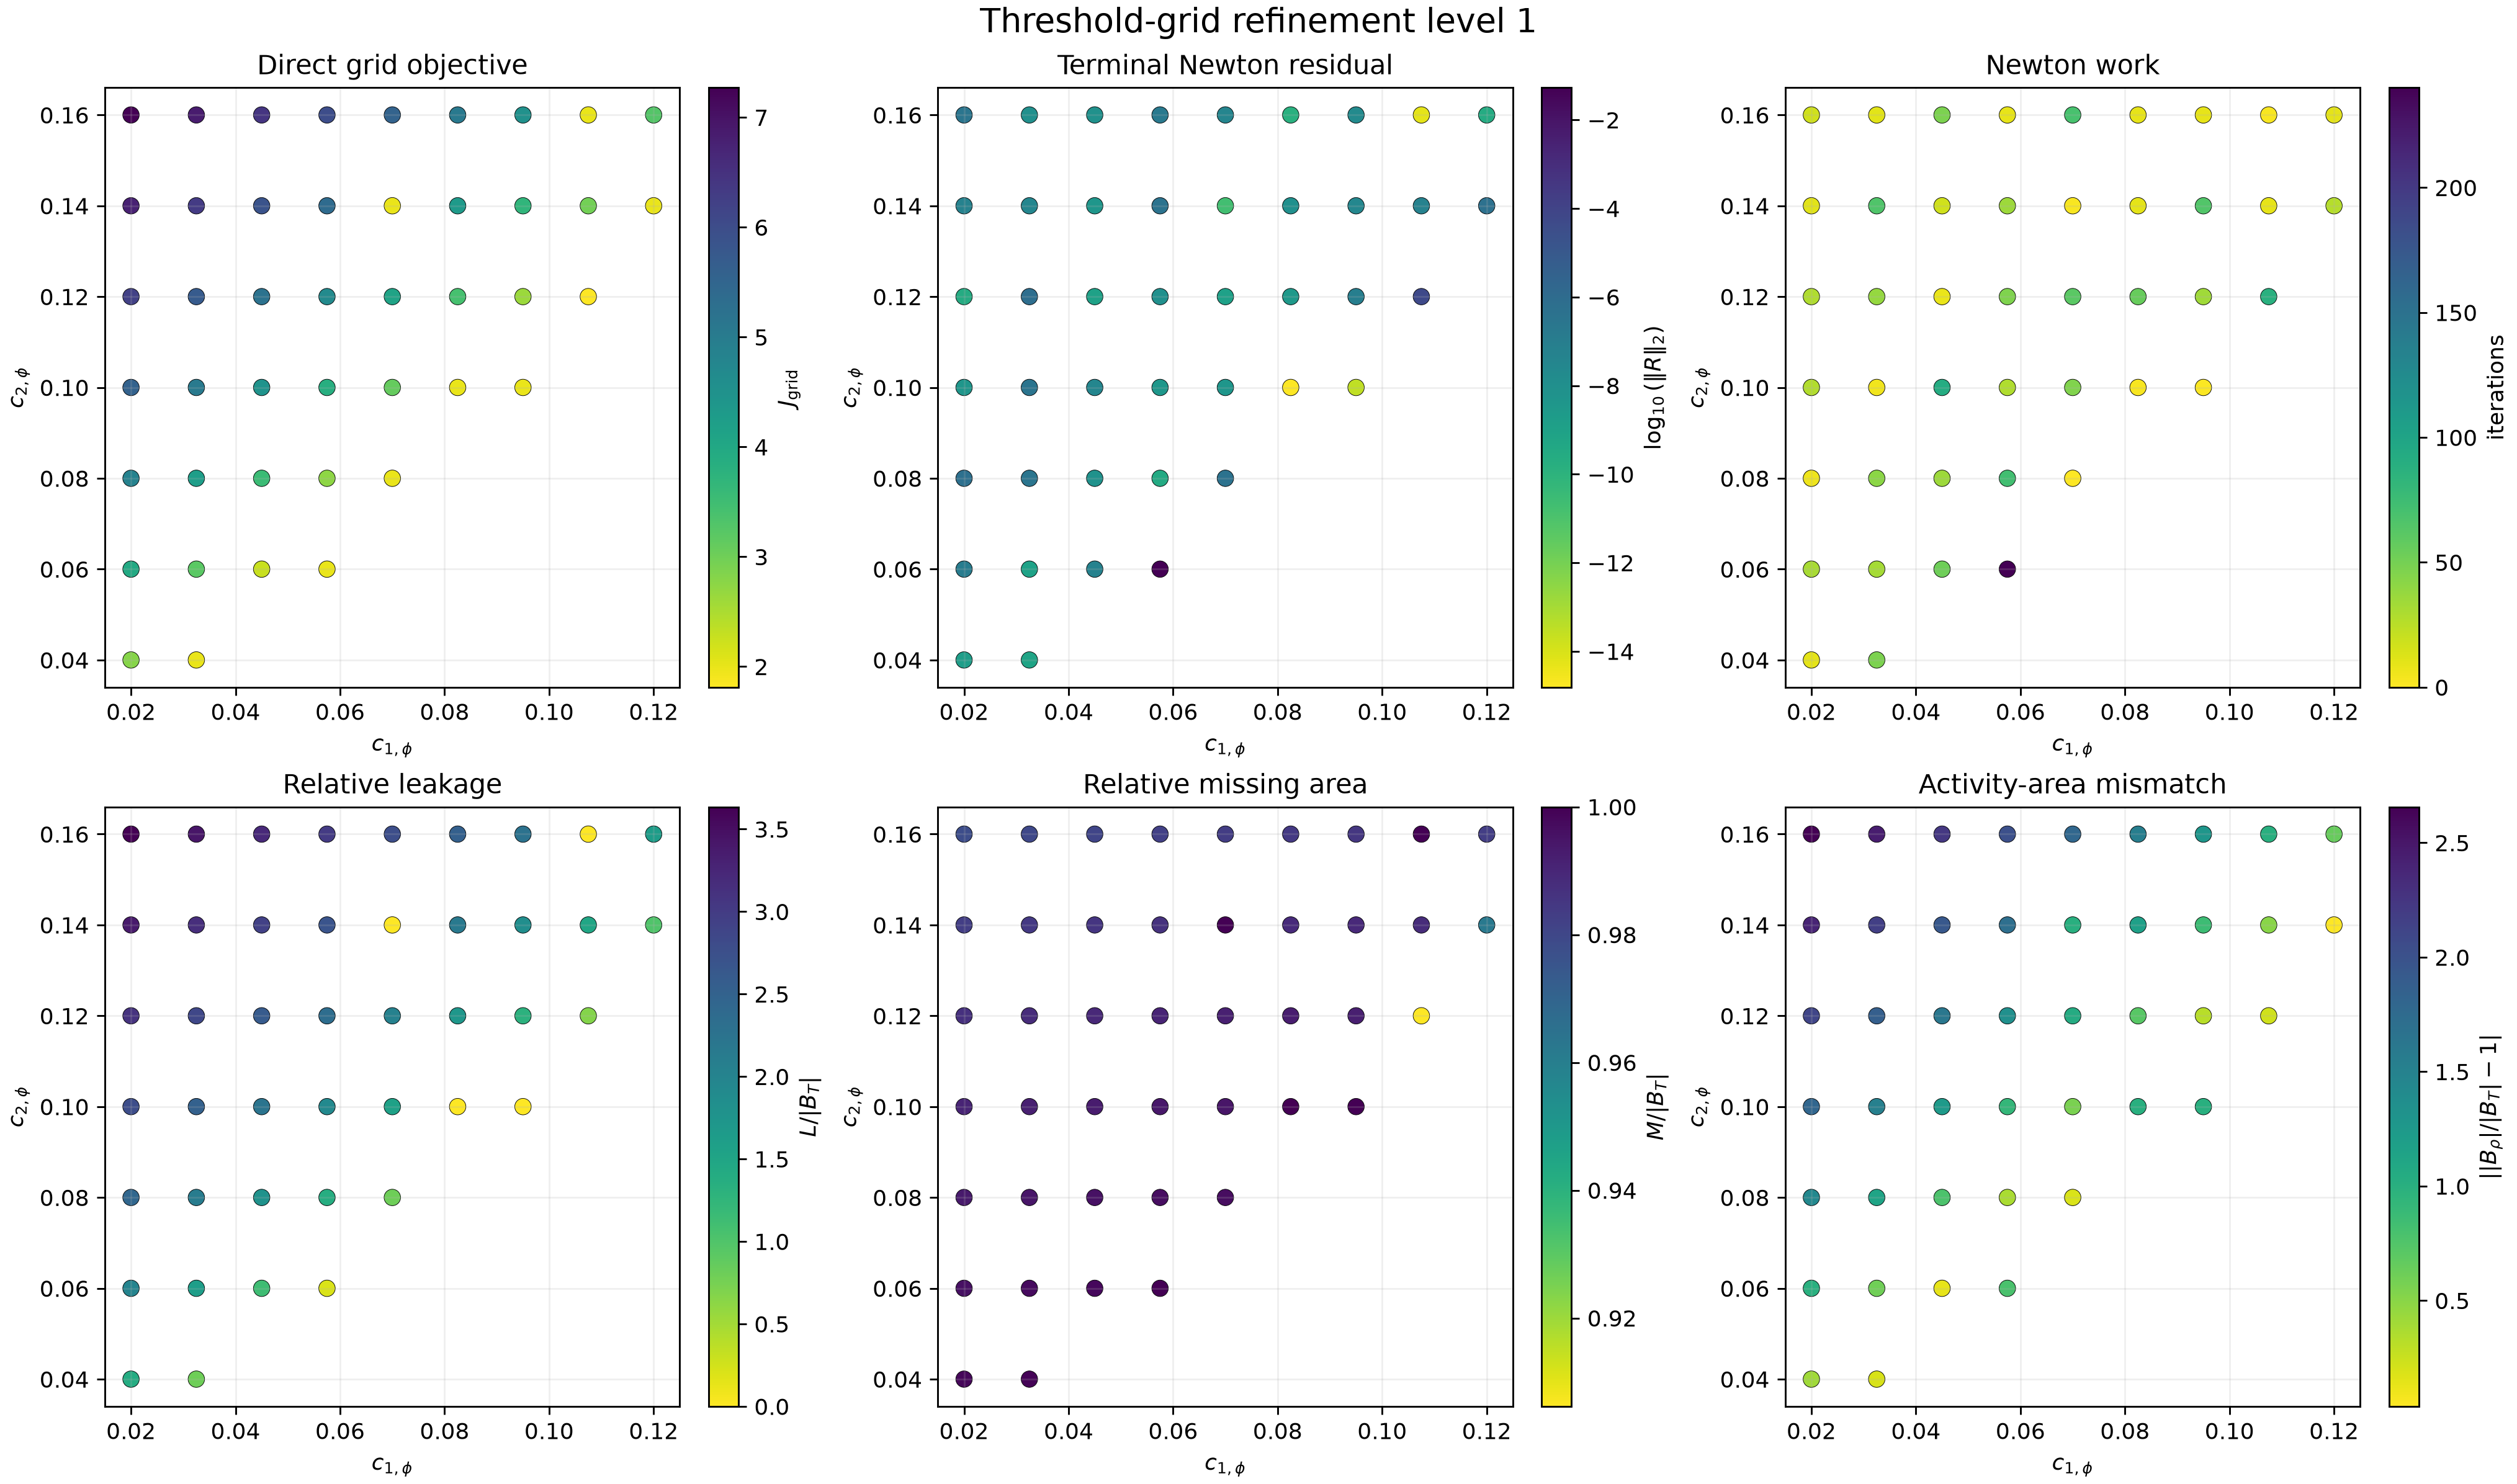
\includegraphics[width=0.97\linewidth]{figures/iter_0p6_0p7_bruteforce_active_eps002_lowdof_grid_level_1.png}
\caption{Fine-grid diagnostics for the corrected ITER search: objective, terminal residual and nonlinear work, leakage, missing area, and activity-area mismatch.  The retained point is PDE-feasible and has two active contours, but its leakage and missing-area errors demonstrate that feasibility is not geometric success.  Data status: actual.}
\label{fig:iter-active-grid-level-one}
\end{figure}
\end{landscape}

\begin{figure}[tbp]
\centering
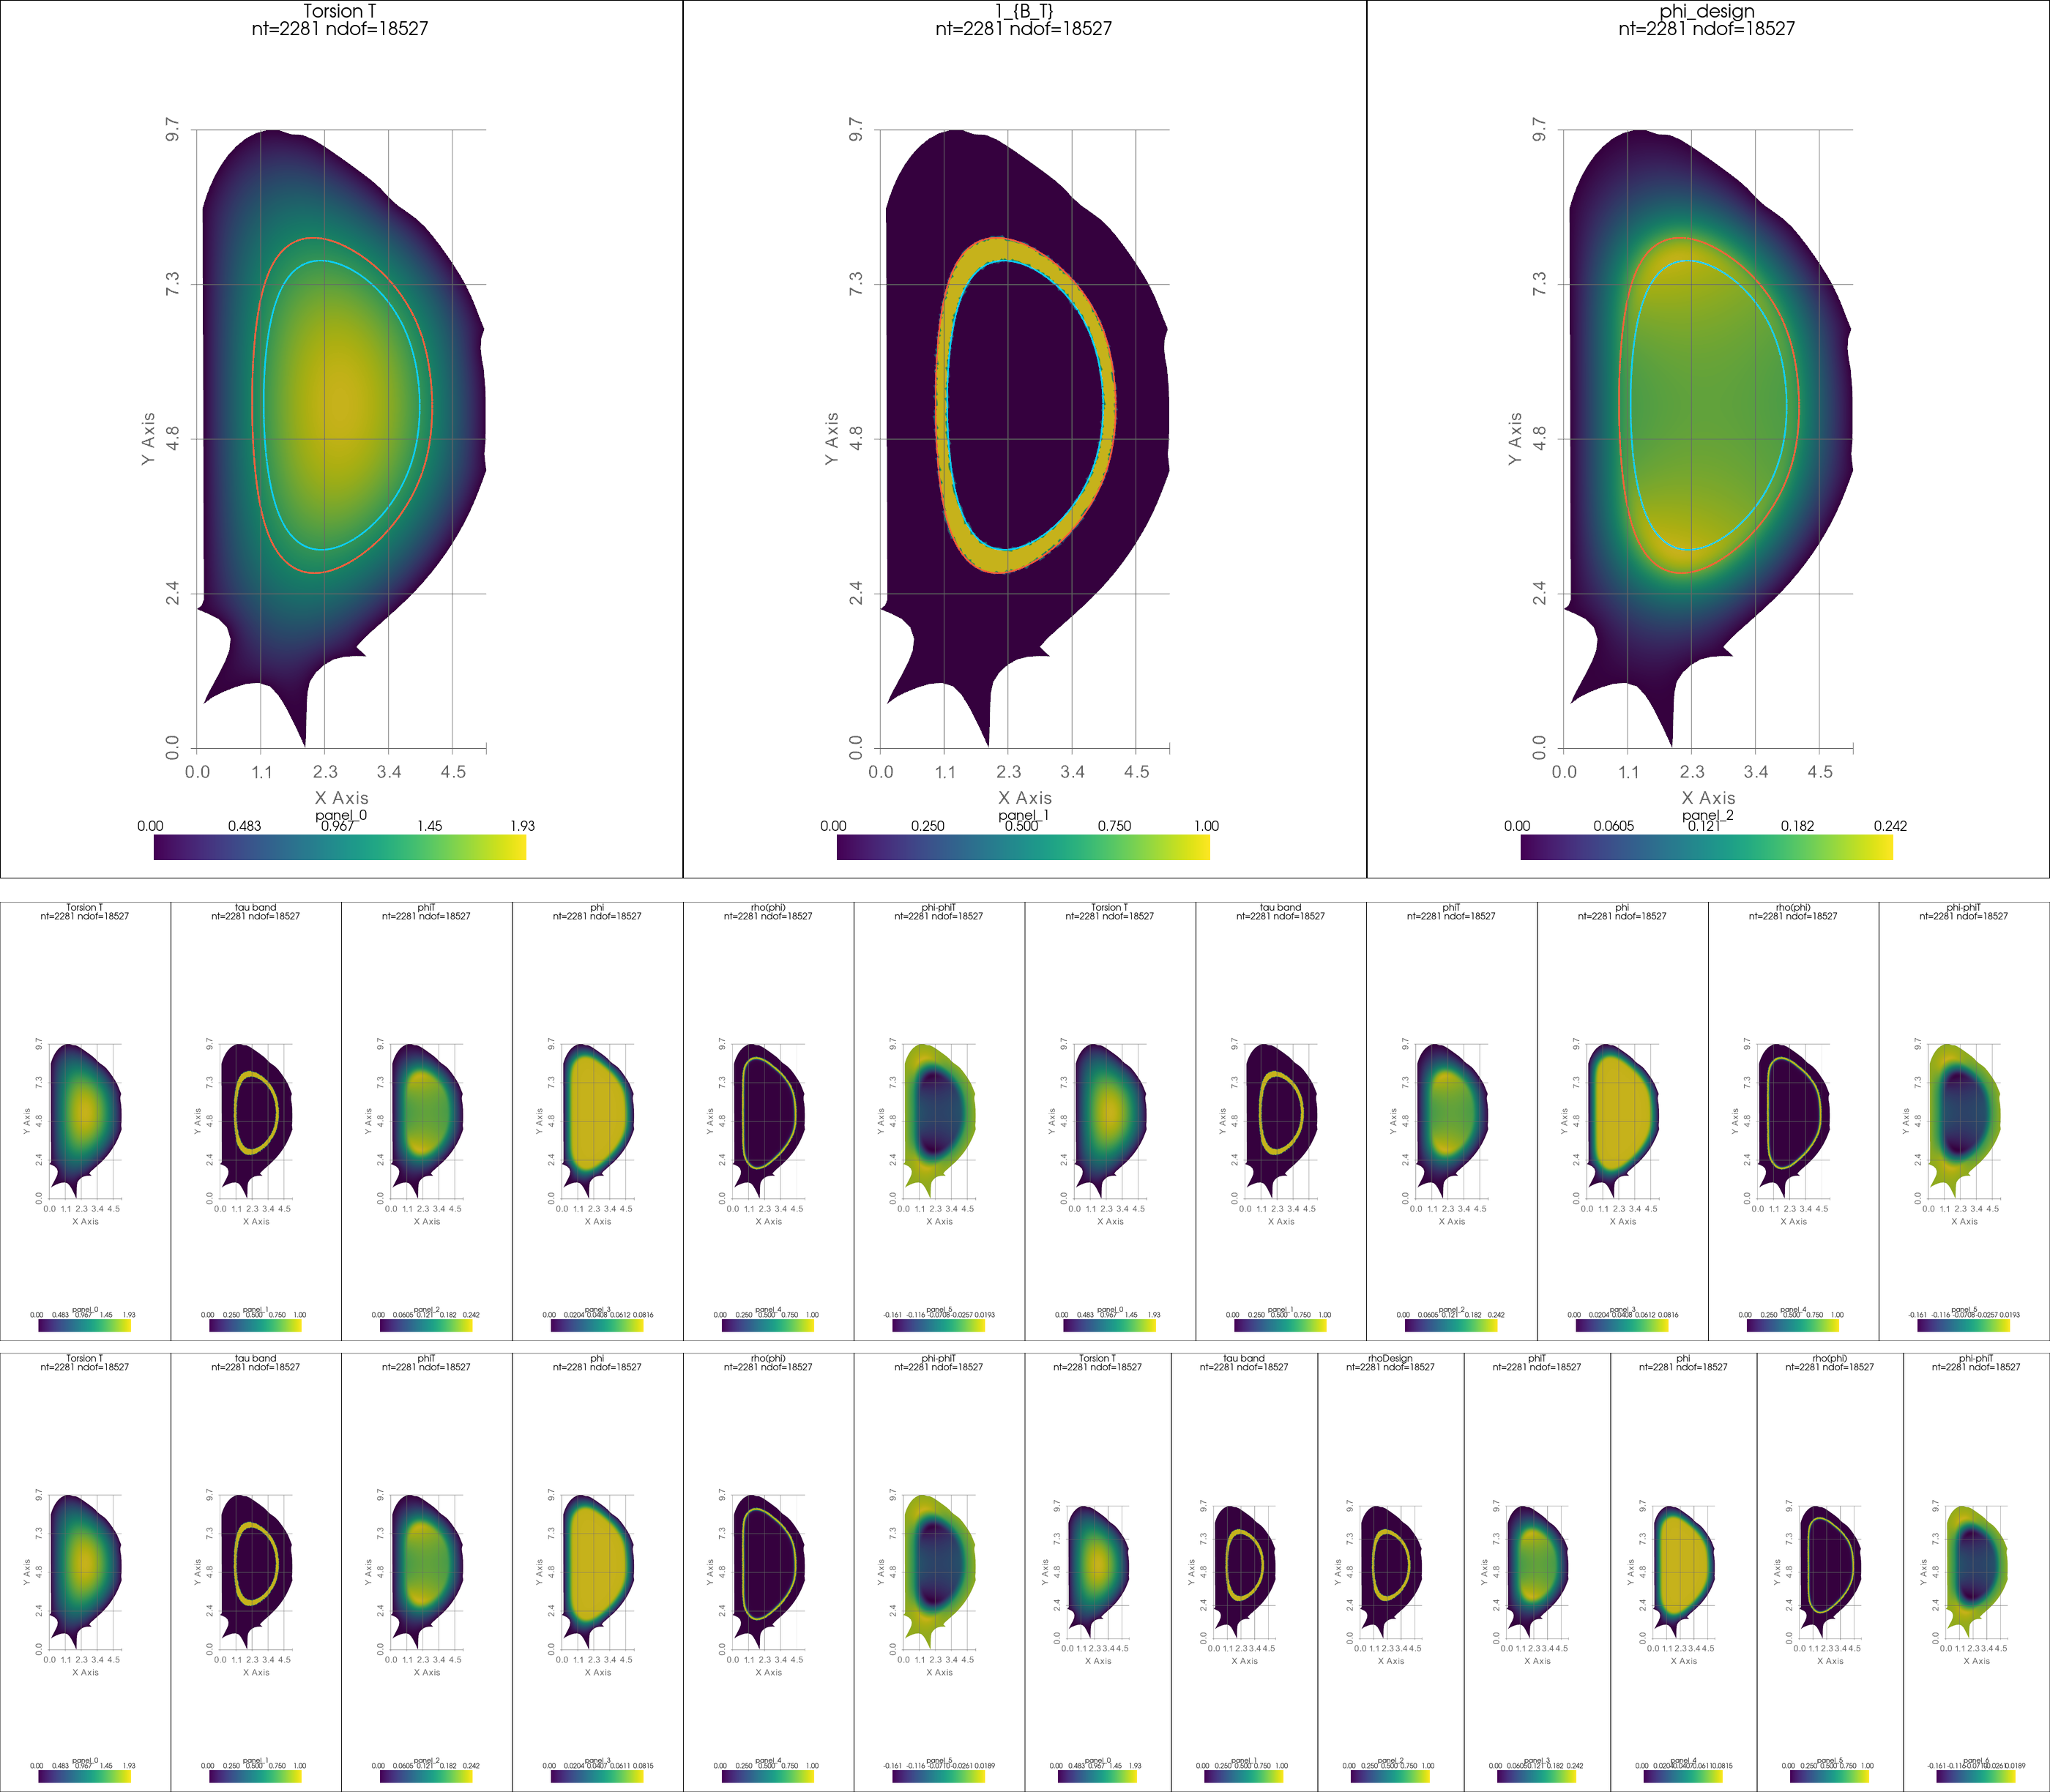
\includegraphics[width=0.93\linewidth,height=0.72\textheight,keepaspectratio]{figures/iter_0p6_0p7_bruteforce_active_eps002_lowdof_storyboard.png}
\caption{Separated design fields and reduced-optimization evolution for the corrected low-DOF ITER run.  The target fields are shown once; later panels retain only the dashed orange target contours and solid blue moving-equilibrium contours.  Rank zero gathers the complete distributed fields, mesh edges are hidden, and all native frames are lossless PNGs.  The conspicuous spatial mismatch is therefore a numerical result rather than a parallel plotting artifact.  Data status: actual; geometrically unsuccessful.}
\label{fig:iter-active-storyboard}
\end{figure}

\subsubsection{Sensitivity and threshold-step audit}

The analytic derivatives were re-derived from
\[
 W(\phi,c_1,c_2,\varepsilon)
 =H_\varepsilon(\phi-c_1)-H_\varepsilon(\phi-c_2).
\]
At fixed \(\varepsilon\),
\(W_\phi=(q_1-q_2)/\varepsilon\),
\(W_{c_1}=-q_1/\varepsilon\), and
\(W_{c_2}=q_2/\varepsilon\); the implementation also includes the two chain
terms generated by
\(\varepsilon=0.02(c_2-c_1)\).  The signs of the state-sensitivity right-hand
side and the direct leakage and missing-area terms agree with the
linearization of \(K\phi-\rho_{\max}W=0\).

The PDE-level audit solves centered perturbed nonlinear problems rather than
checking only symbolic expressions.  At a local-width-scaled perturbation
\(h=10^{-7}\), both perturbed states reached the requested residual.  For
\(c_1\), the relative state errors were
\(3.32\times10^{-5}\) in \(L^2\) and \(3.64\times10^{-5}\) in \(H^1\);
the leakage and missing-gradient errors were \(1.05\times10^{-5}\) and
\(5.87\times10^{-6}\).  For \(c_2\), the corresponding values were
\(1.57\times10^{-5}\), \(2.15\times10^{-5}\),
\(4.97\times10^{-6}\), and \(6.52\times10^{-6}\).
This verifies the implemented sensitivities to the accuracy supported by the
nonlinear perturbed solves.

The audit nevertheless exposed two optimizer bugs.  First, branch retention
had been normalized by \(\int W_{\rm ref}\) rather than
\(\int W_{\rm ref}^2\), so even an unchanged diffuse state could score below
the acceptance threshold.  It is now
\[
 \eta_{\rm branch}
 =\frac{\int_\Omega W_{\rm trial}W_{\rm ref}\,dx}
        {\int_\Omega W_{\rm ref}^{\,2}\,dx},
\]
which gives one for an unchanged state.  Second, the standalone reduced
optimizer could evaluate sensitivities after an unresolved base Newton
solve.  It now records \texttt{INNER\_NEWTON\_UNRESOLVED}, skips the
threshold step, and proceeds to the final projection.  Base and trial
thresholds, residuals, metrics, and each acceptance predicate are stored in
separate CSV columns, eliminating the previous mixed-iterate diagnostics.

\begin{figure}[tbp]
\centering
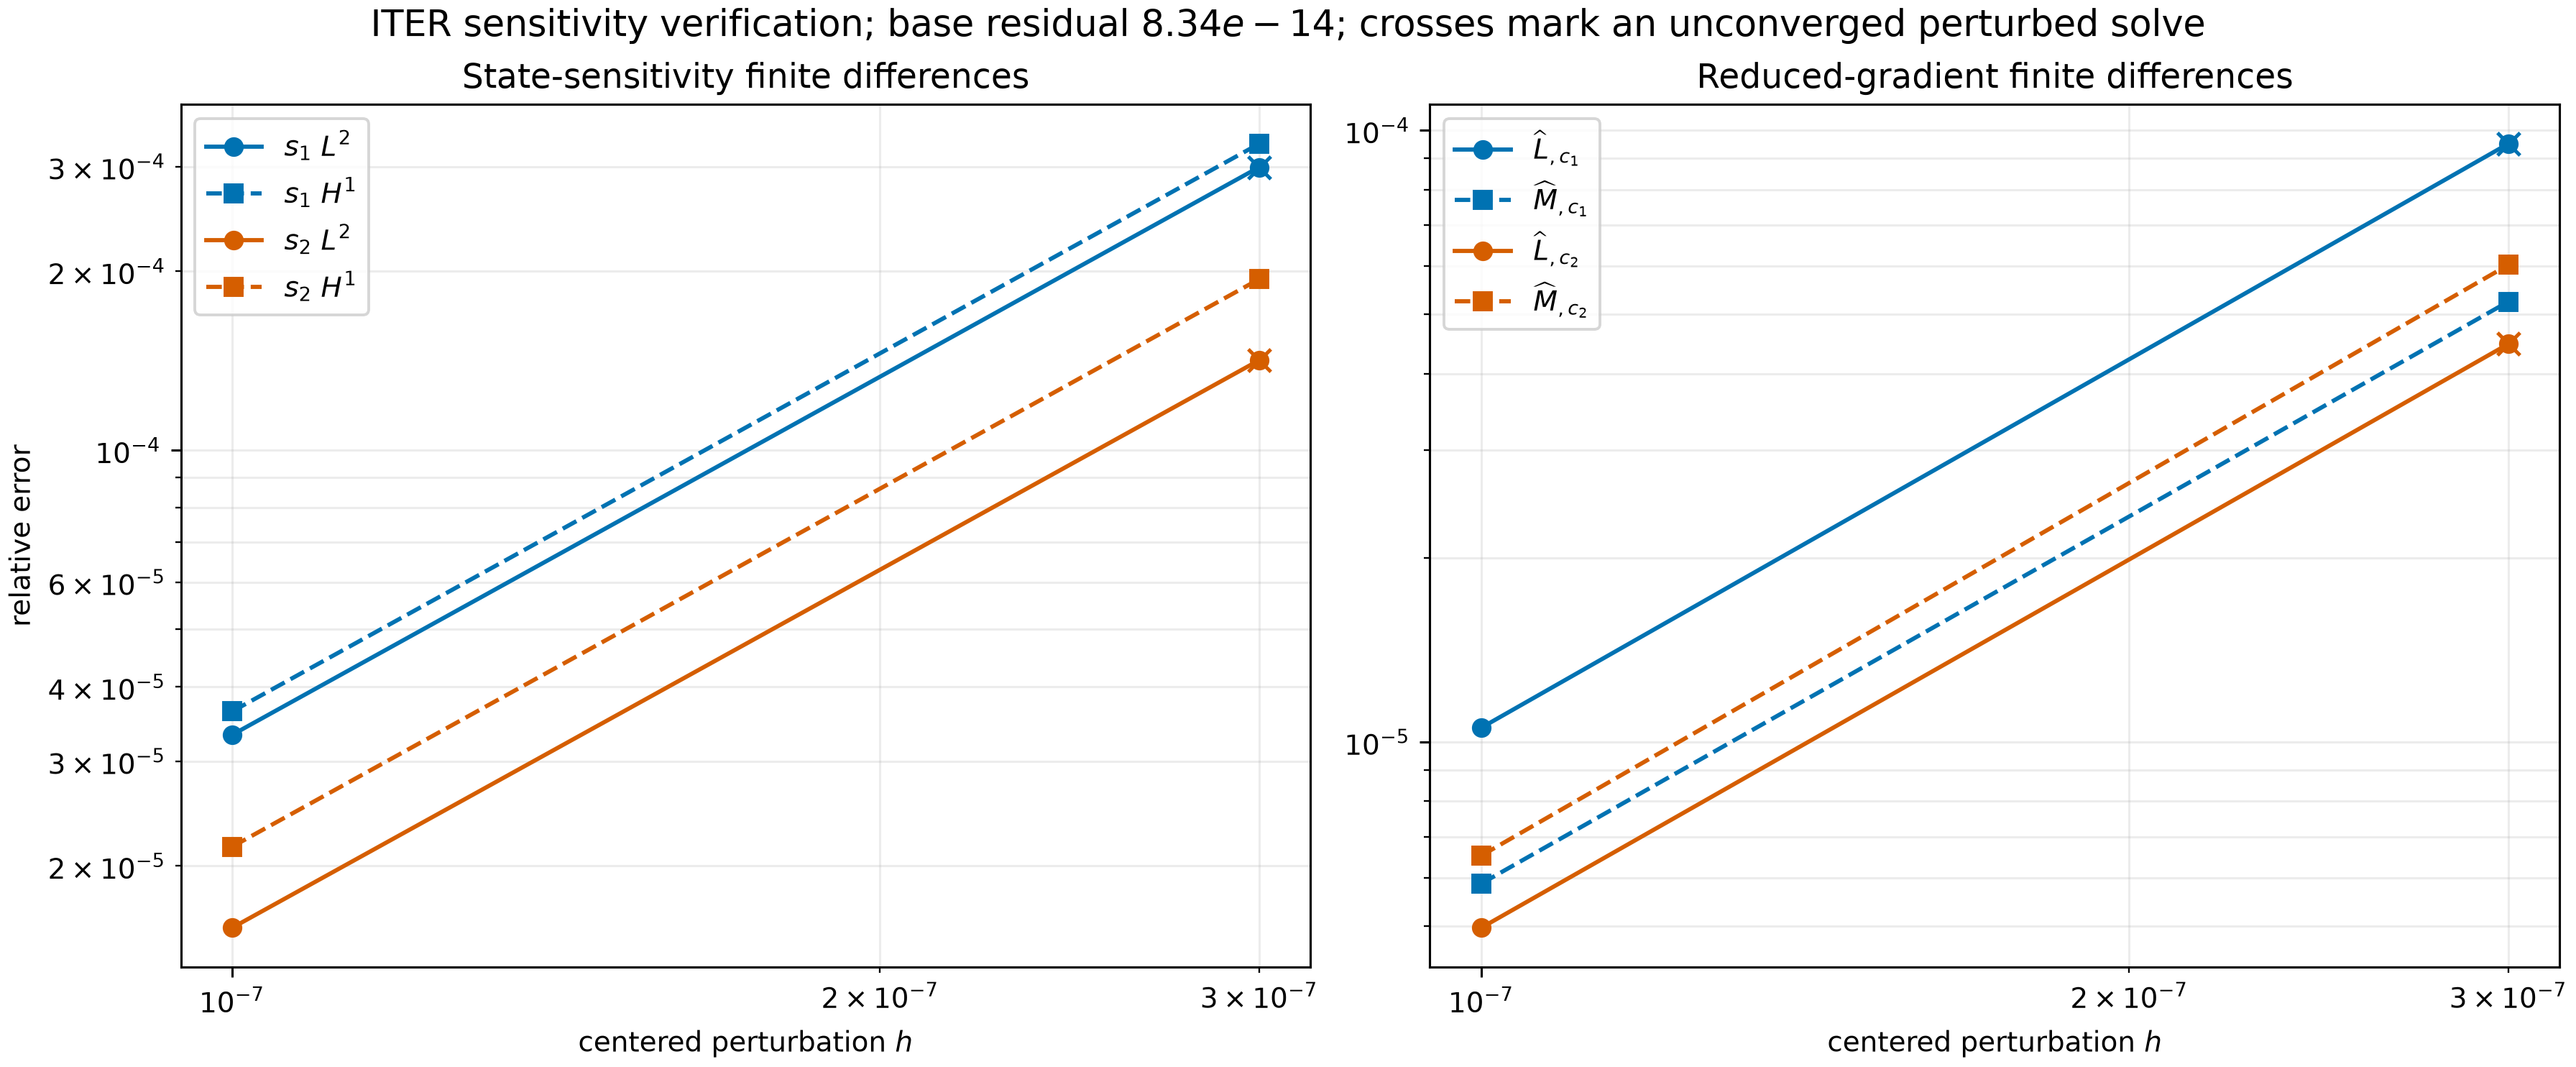
\includegraphics[width=0.95\linewidth]{figures/iter_0p6_0p7_bruteforce_active_eps002_lowdof_sensitivity_finite_difference.png}
\caption{PDE-level centered finite-difference verification of both state sensitivities and both reduced gradients.  Crosses identify perturbations whose auxiliary Newton solve did not satisfy the deliberately stricter audit criterion; they are retained and are not used as correctness evidence.  The smallest valid perturbation agrees with the analytic derivatives to between \(5\times10^{-6}\) and \(4\times10^{-5}\).  Data status: actual.}
\label{fig:iter-active-sensitivity-check}
\end{figure}

\begin{figure}[tbp]
\centering
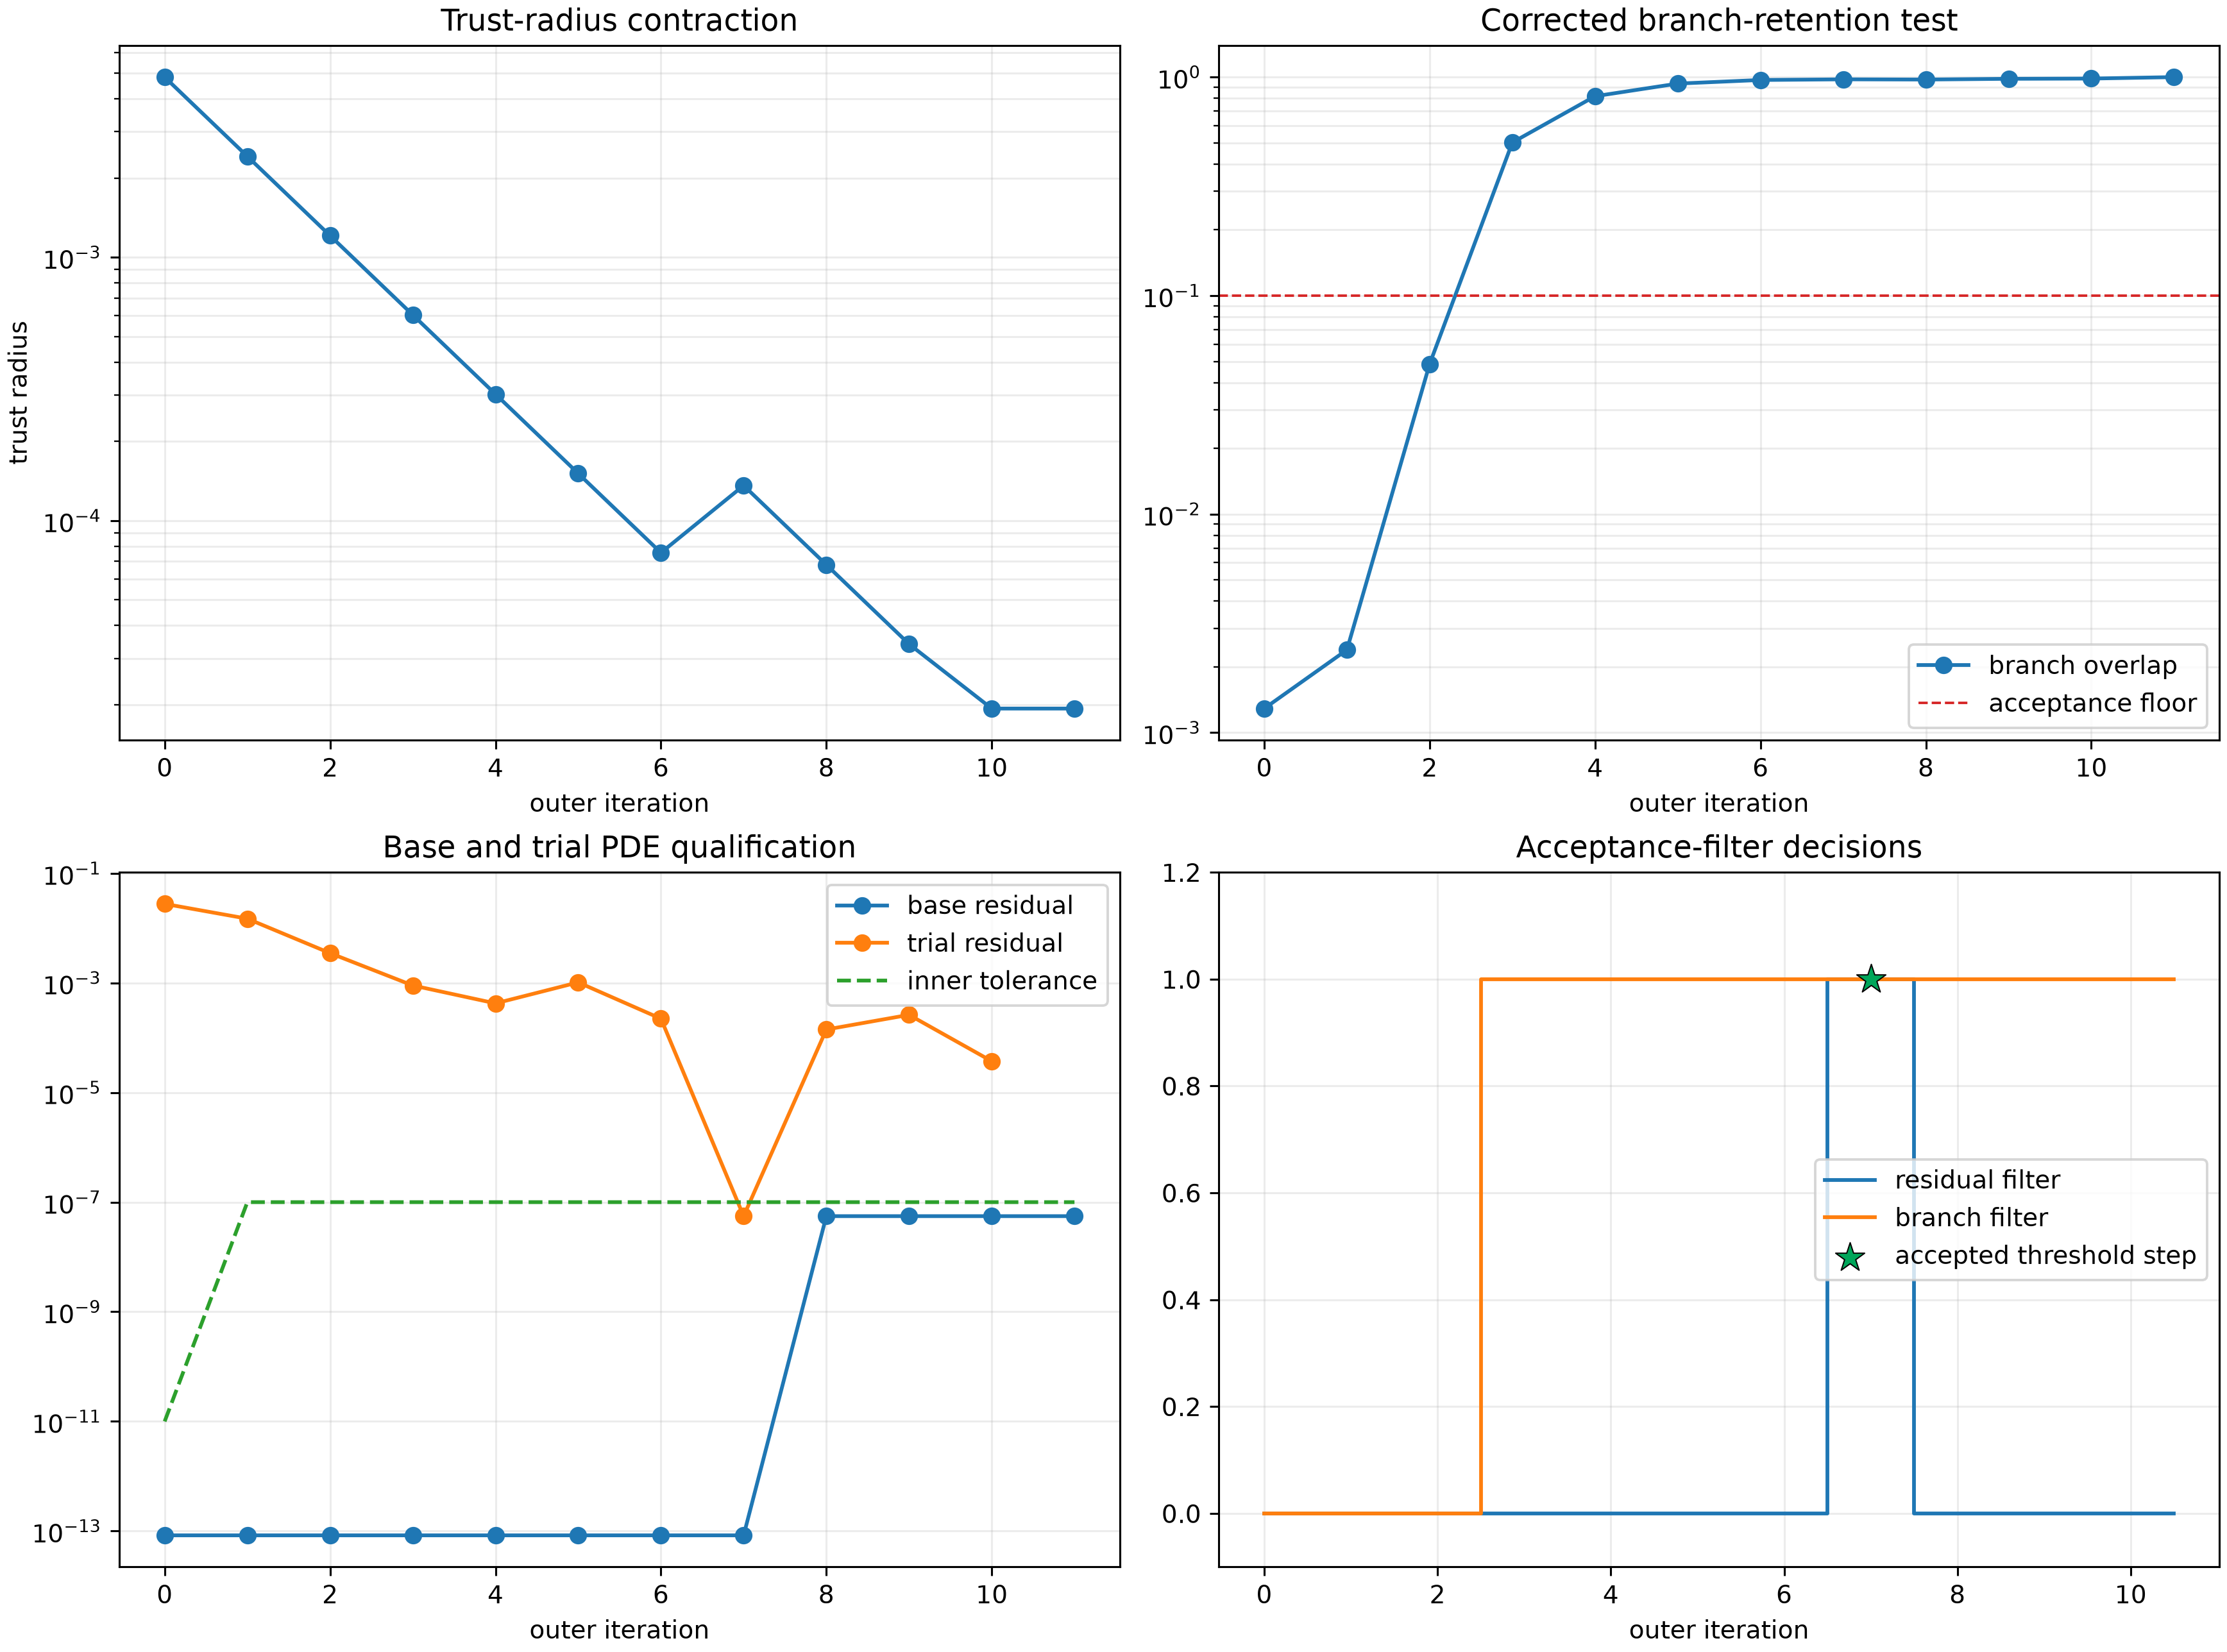
\includegraphics[width=0.97\linewidth,height=0.70\textheight,keepaspectratio]{figures/iter_0p6_0p7_bruteforce_active_eps002_lowdof_trial_acceptance.png}
\caption{Threshold-trial qualification after correcting branch normalization.  The first large trials fail both the inexact residual criterion and genuine branch retention, whereas a sufficiently contracted trial is accepted.  Each panel is computed from the trial state, not from a mixture of base and accepted iterates.  Data status: actual.}
\label{fig:iter-active-trial-acceptance}
\end{figure}

The optimizer accepted one contracted update at outer iteration 7 and moved
the thresholds to \((0.0700538,0.0799470)\).  Subsequent contractions reached
the step floor.  The final exact projection has residual
\(4.40\times10^{-12}\): this satisfies the study's \(10^{-11}\) PDE
criterion, although it is correctly marked as missing the separately
requested \(10^{-12}\) final-projection target.  The geometry remains
unsuccessful, with \(L_{\rm rel}=0.80231\),
\(M_{\rm rel}=0.99667\), certified-area ratio \(0.63539\), and active-set
Jaccard index \(0.00260\).  Correcting the acceptance logic therefore permits
a legitimate step, but does not turn this branch into the desired ITER band.

\begin{landscape}
\begin{figure}[tbp]
\centering
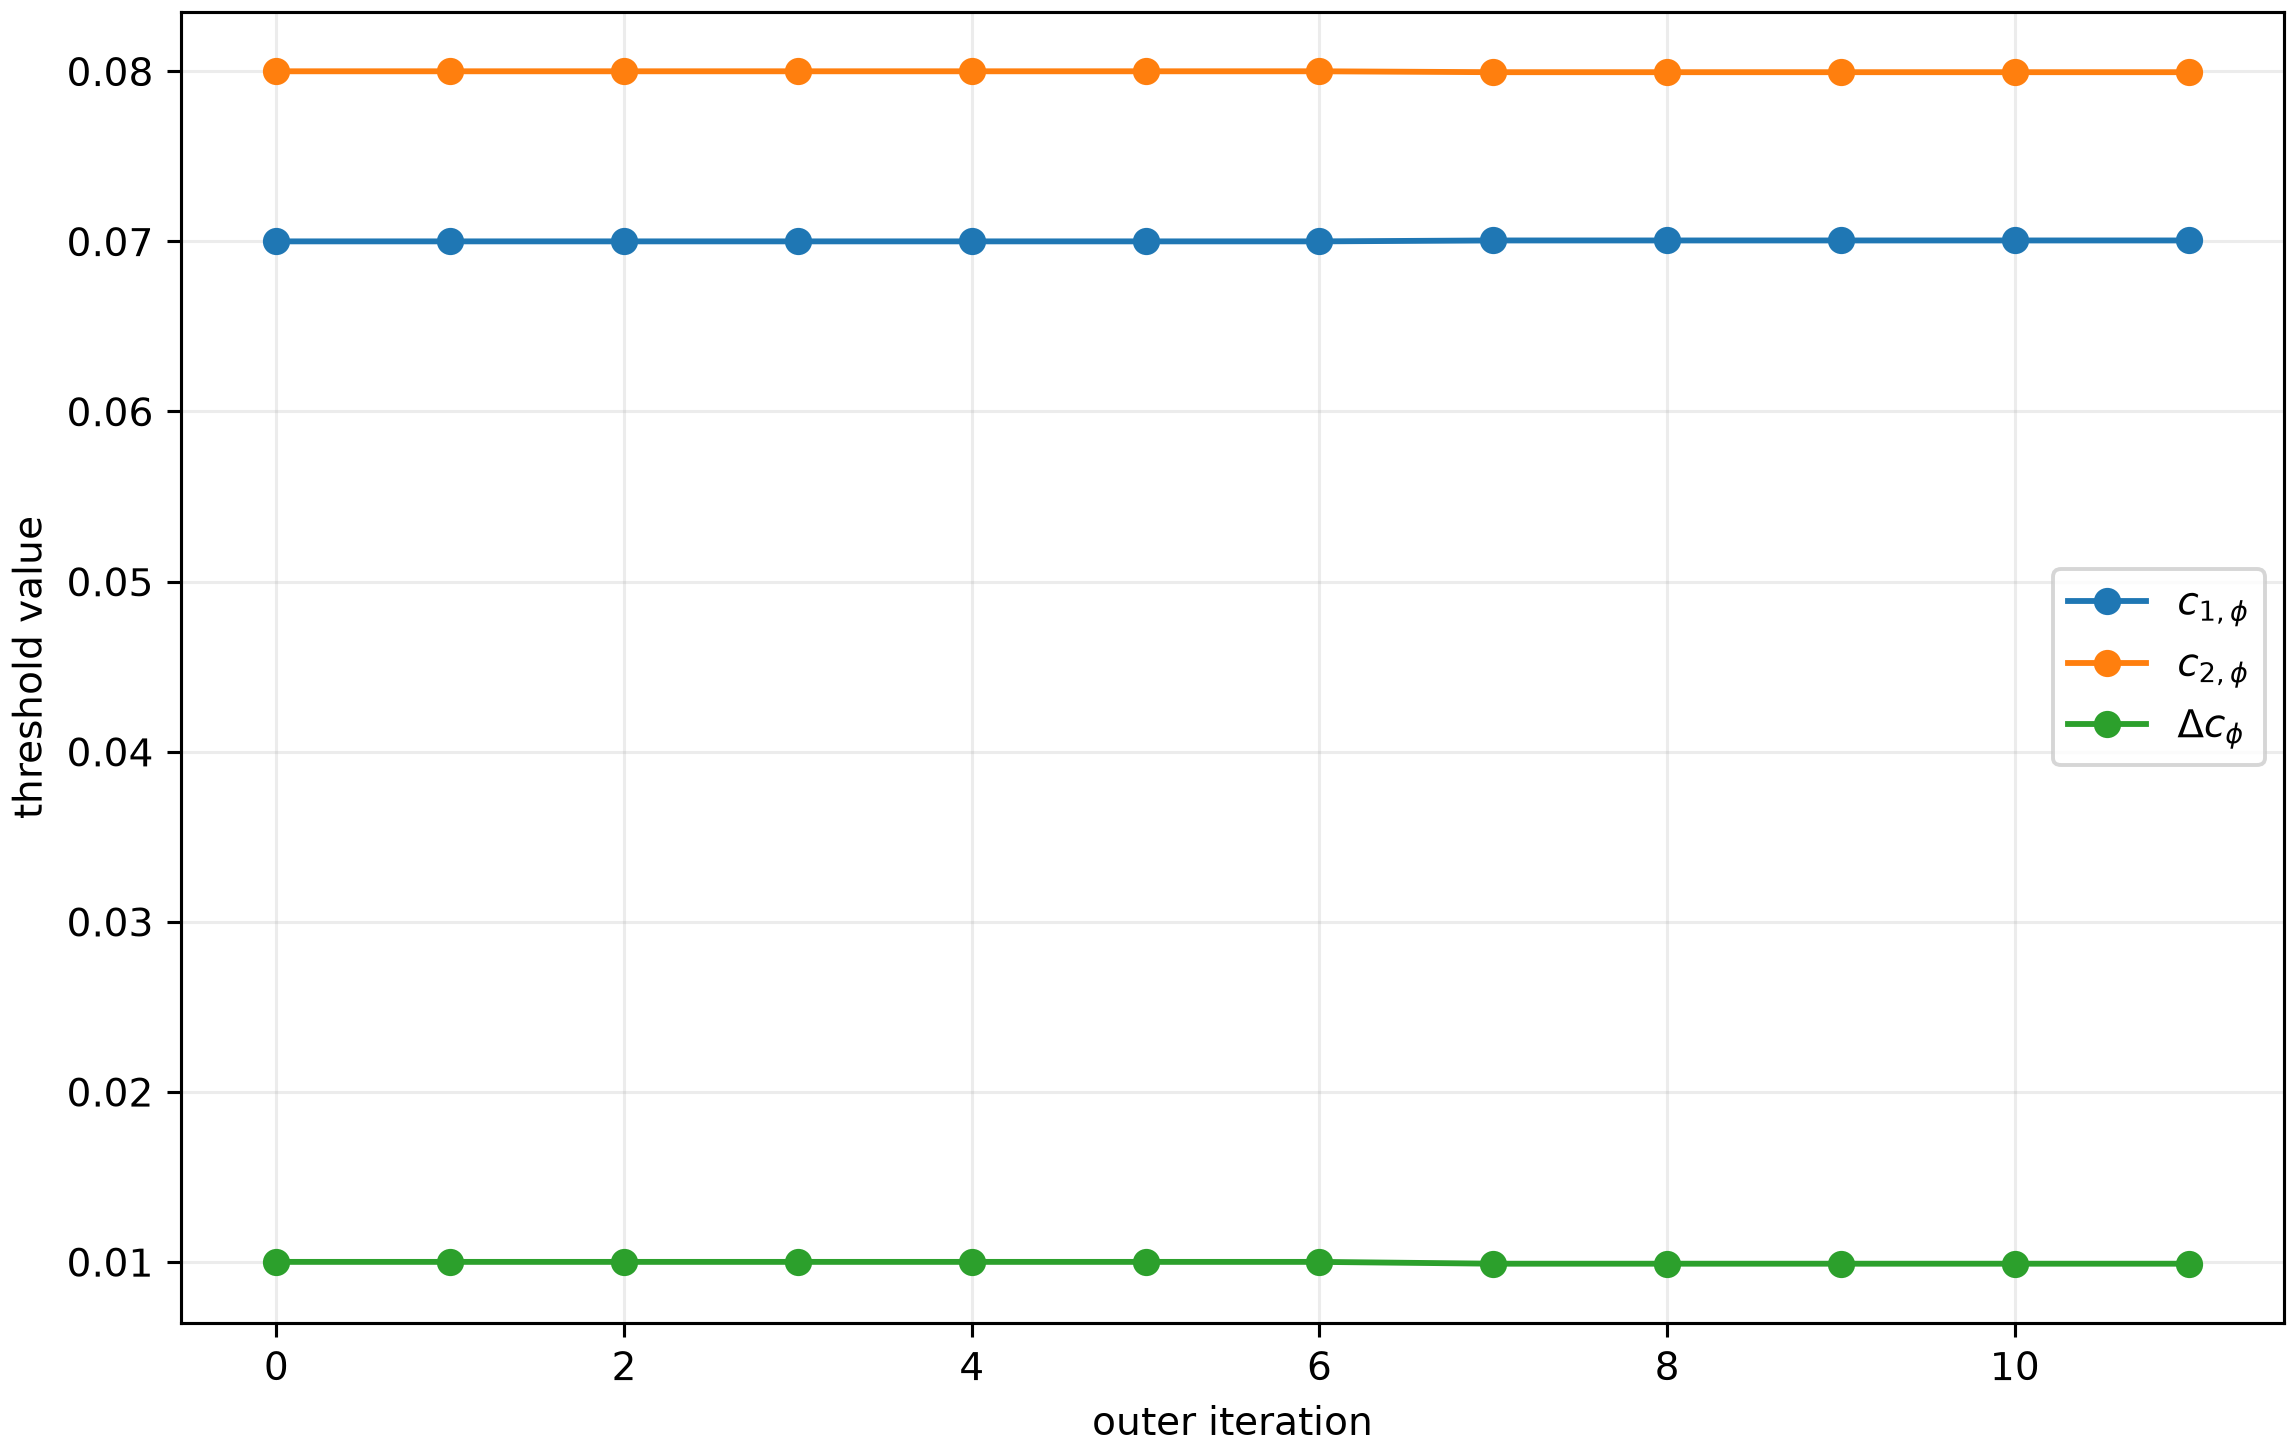
\includegraphics[width=0.49\linewidth]{figures/iter_0p6_0p7_bruteforce_active_eps002_lowdof_threshold_convergence.png}
\hfill
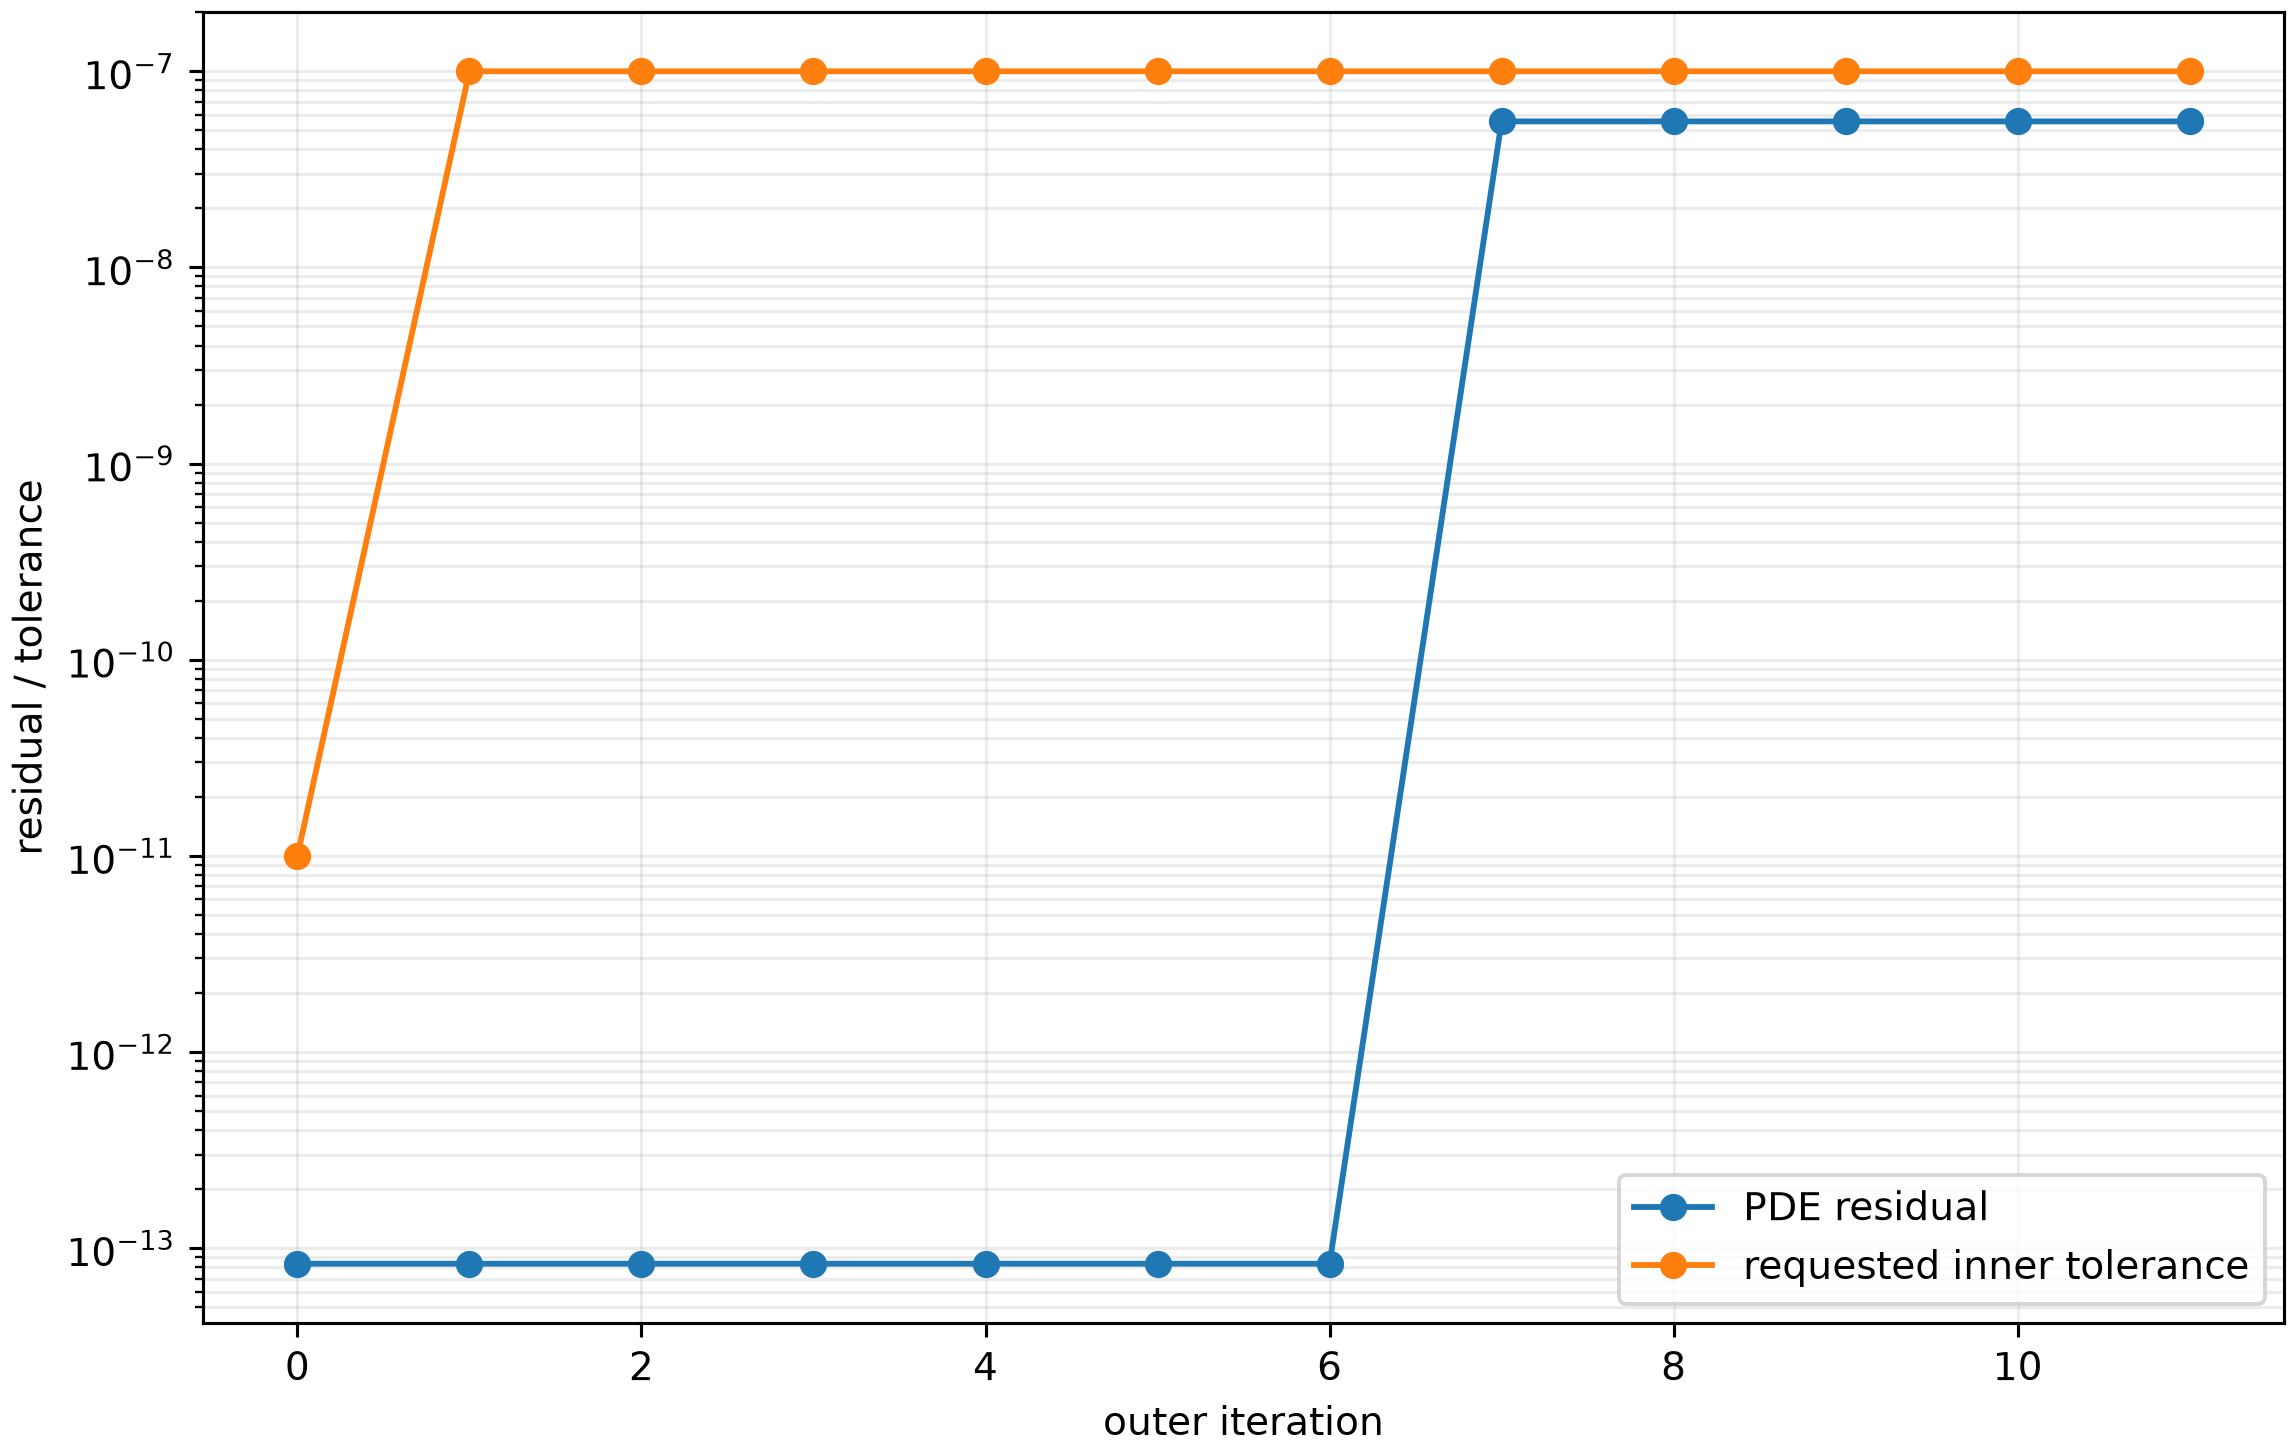
\includegraphics[width=0.49\linewidth]{figures/iter_0p6_0p7_bruteforce_active_eps002_lowdof_pde_residual_convergence.png}
\caption{Threshold-space motion (left) and nonlinear residual history (right).  The threshold pair changes only after sufficient trust-region contraction; the final projection is below \(10^{-11}\), but the geometric objective plateaus.  Data status: actual; PDE-qualified geometric failure.}
\label{fig:iter-active-threshold-and-residual}
\end{figure}
\end{landscape}

\subsubsection{Does a smaller equilibrium smoothing width help?}

To isolate smoothing from threshold selection, we solved the same
\((0.07,0.08)\) pair on the same mesh at ratios \(0.04\), \(0.02\), and
\(0.01\), using tight MUMPS projections.  All three states are PDE-converged.
The result is monotone but unfavorable:
\[
\begin{array}{c@{\qquad}ccc}
\toprule
\varepsilon_\phi/\Delta c_\phi
 & L_{\rm rel} & M_{\rm rel} & J_{\rm active}\\
\midrule
0.04 & 0.80489 & 0.99385 & 0.00376\\
0.02 & 0.80772 & 0.99672 & 0.00233\\
0.01 & 0.80959 & 0.99827 & 0.00123\\
\bottomrule
\end{array}
\]
Thus decreasing \(\varepsilon_\phi\) sharpens the same displaced equilibrium
branch and makes both area coverage and active-set overlap worse.  It cannot,
by itself, make this equilibrium fit inside the target band.  The unresolved
issue is branch discovery or target attainability at this discretization,
not diffuse-interface thickness.

\begin{figure}[tbp]
\centering
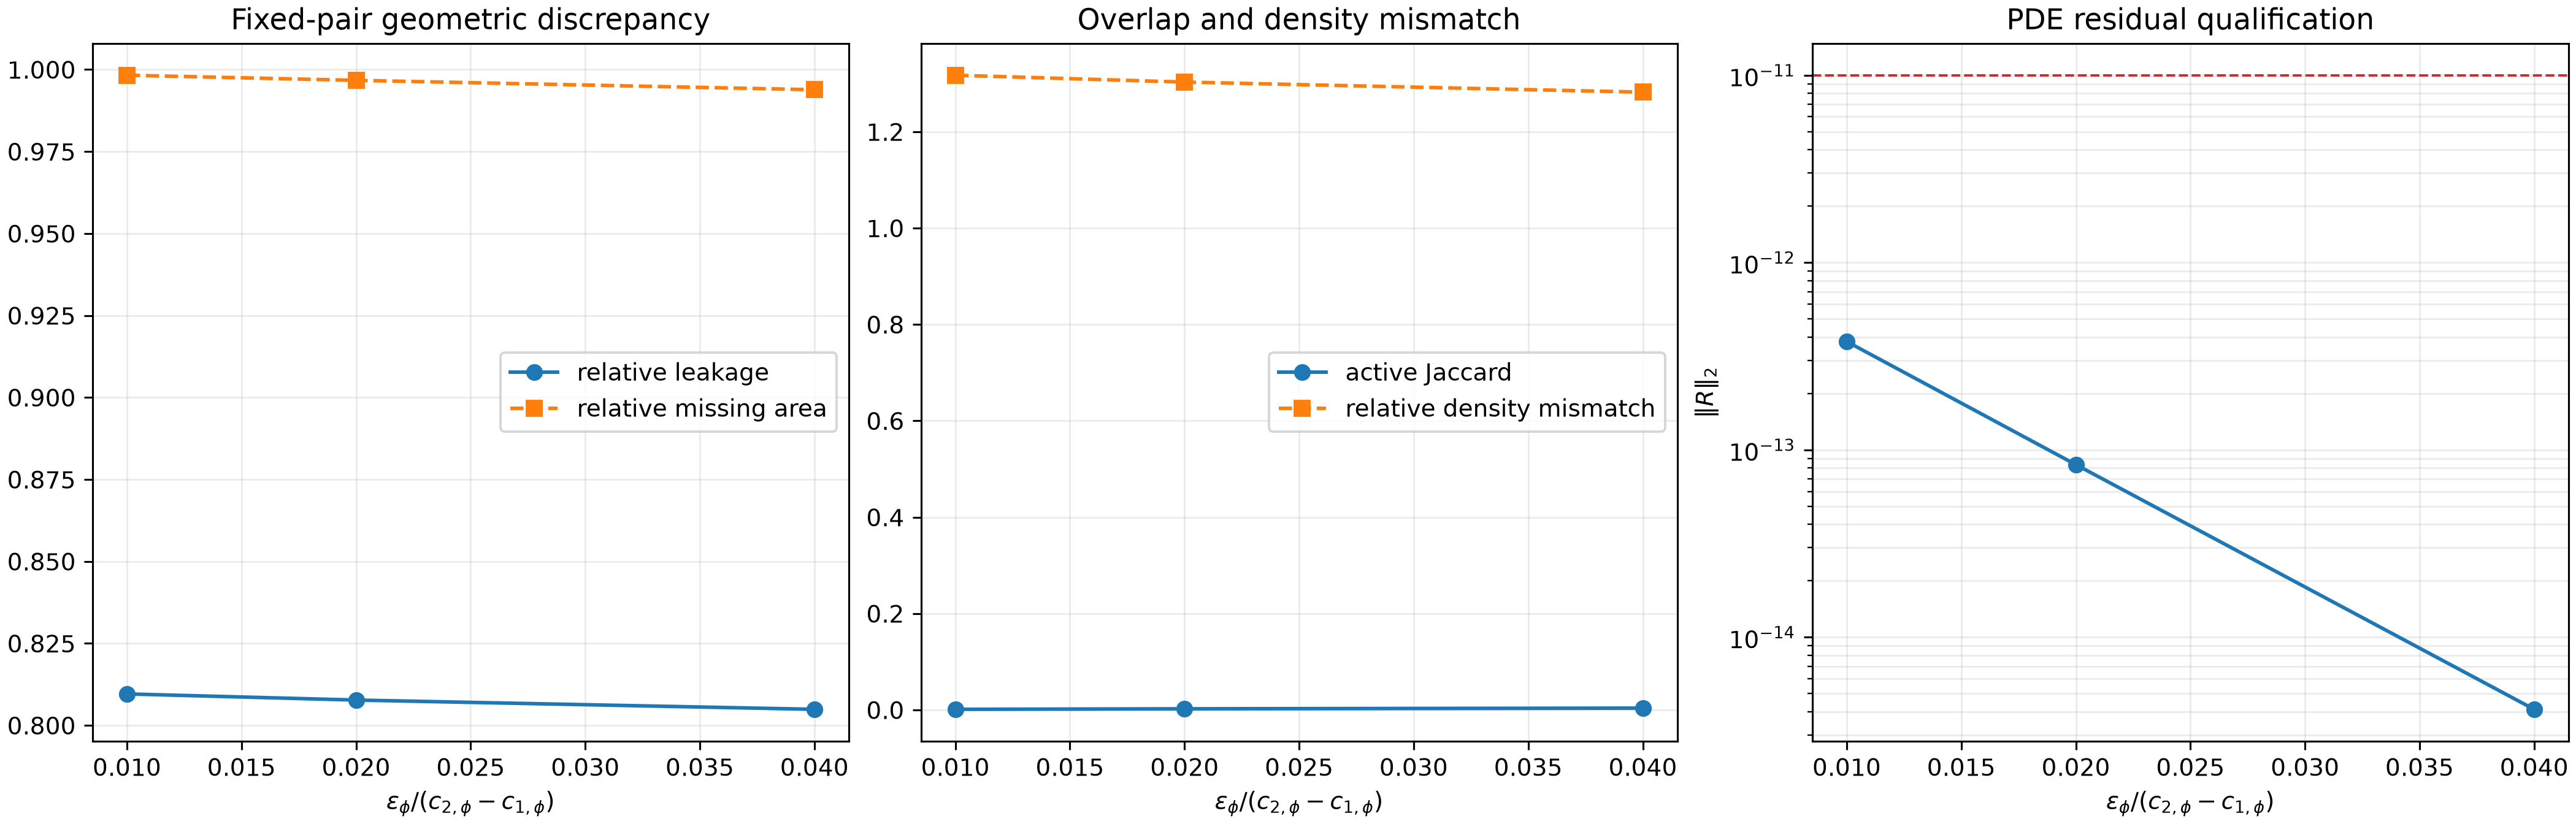
\includegraphics[width=0.97\linewidth]{figures/iter_0p6_0p7_bruteforce_active_eps002_lowdof_epsilon_fixed_pair.png}
\caption{Matched-pair smoothing control.  Lowering the relative equilibrium smoothing width increases leakage and missing area, decreases active-set Jaccard overlap, and leaves all PDE residuals qualified.  Data status: actual.}
\label{fig:iter-active-epsilon-control}
\end{figure}

\begin{figure}[tbp]
\centering
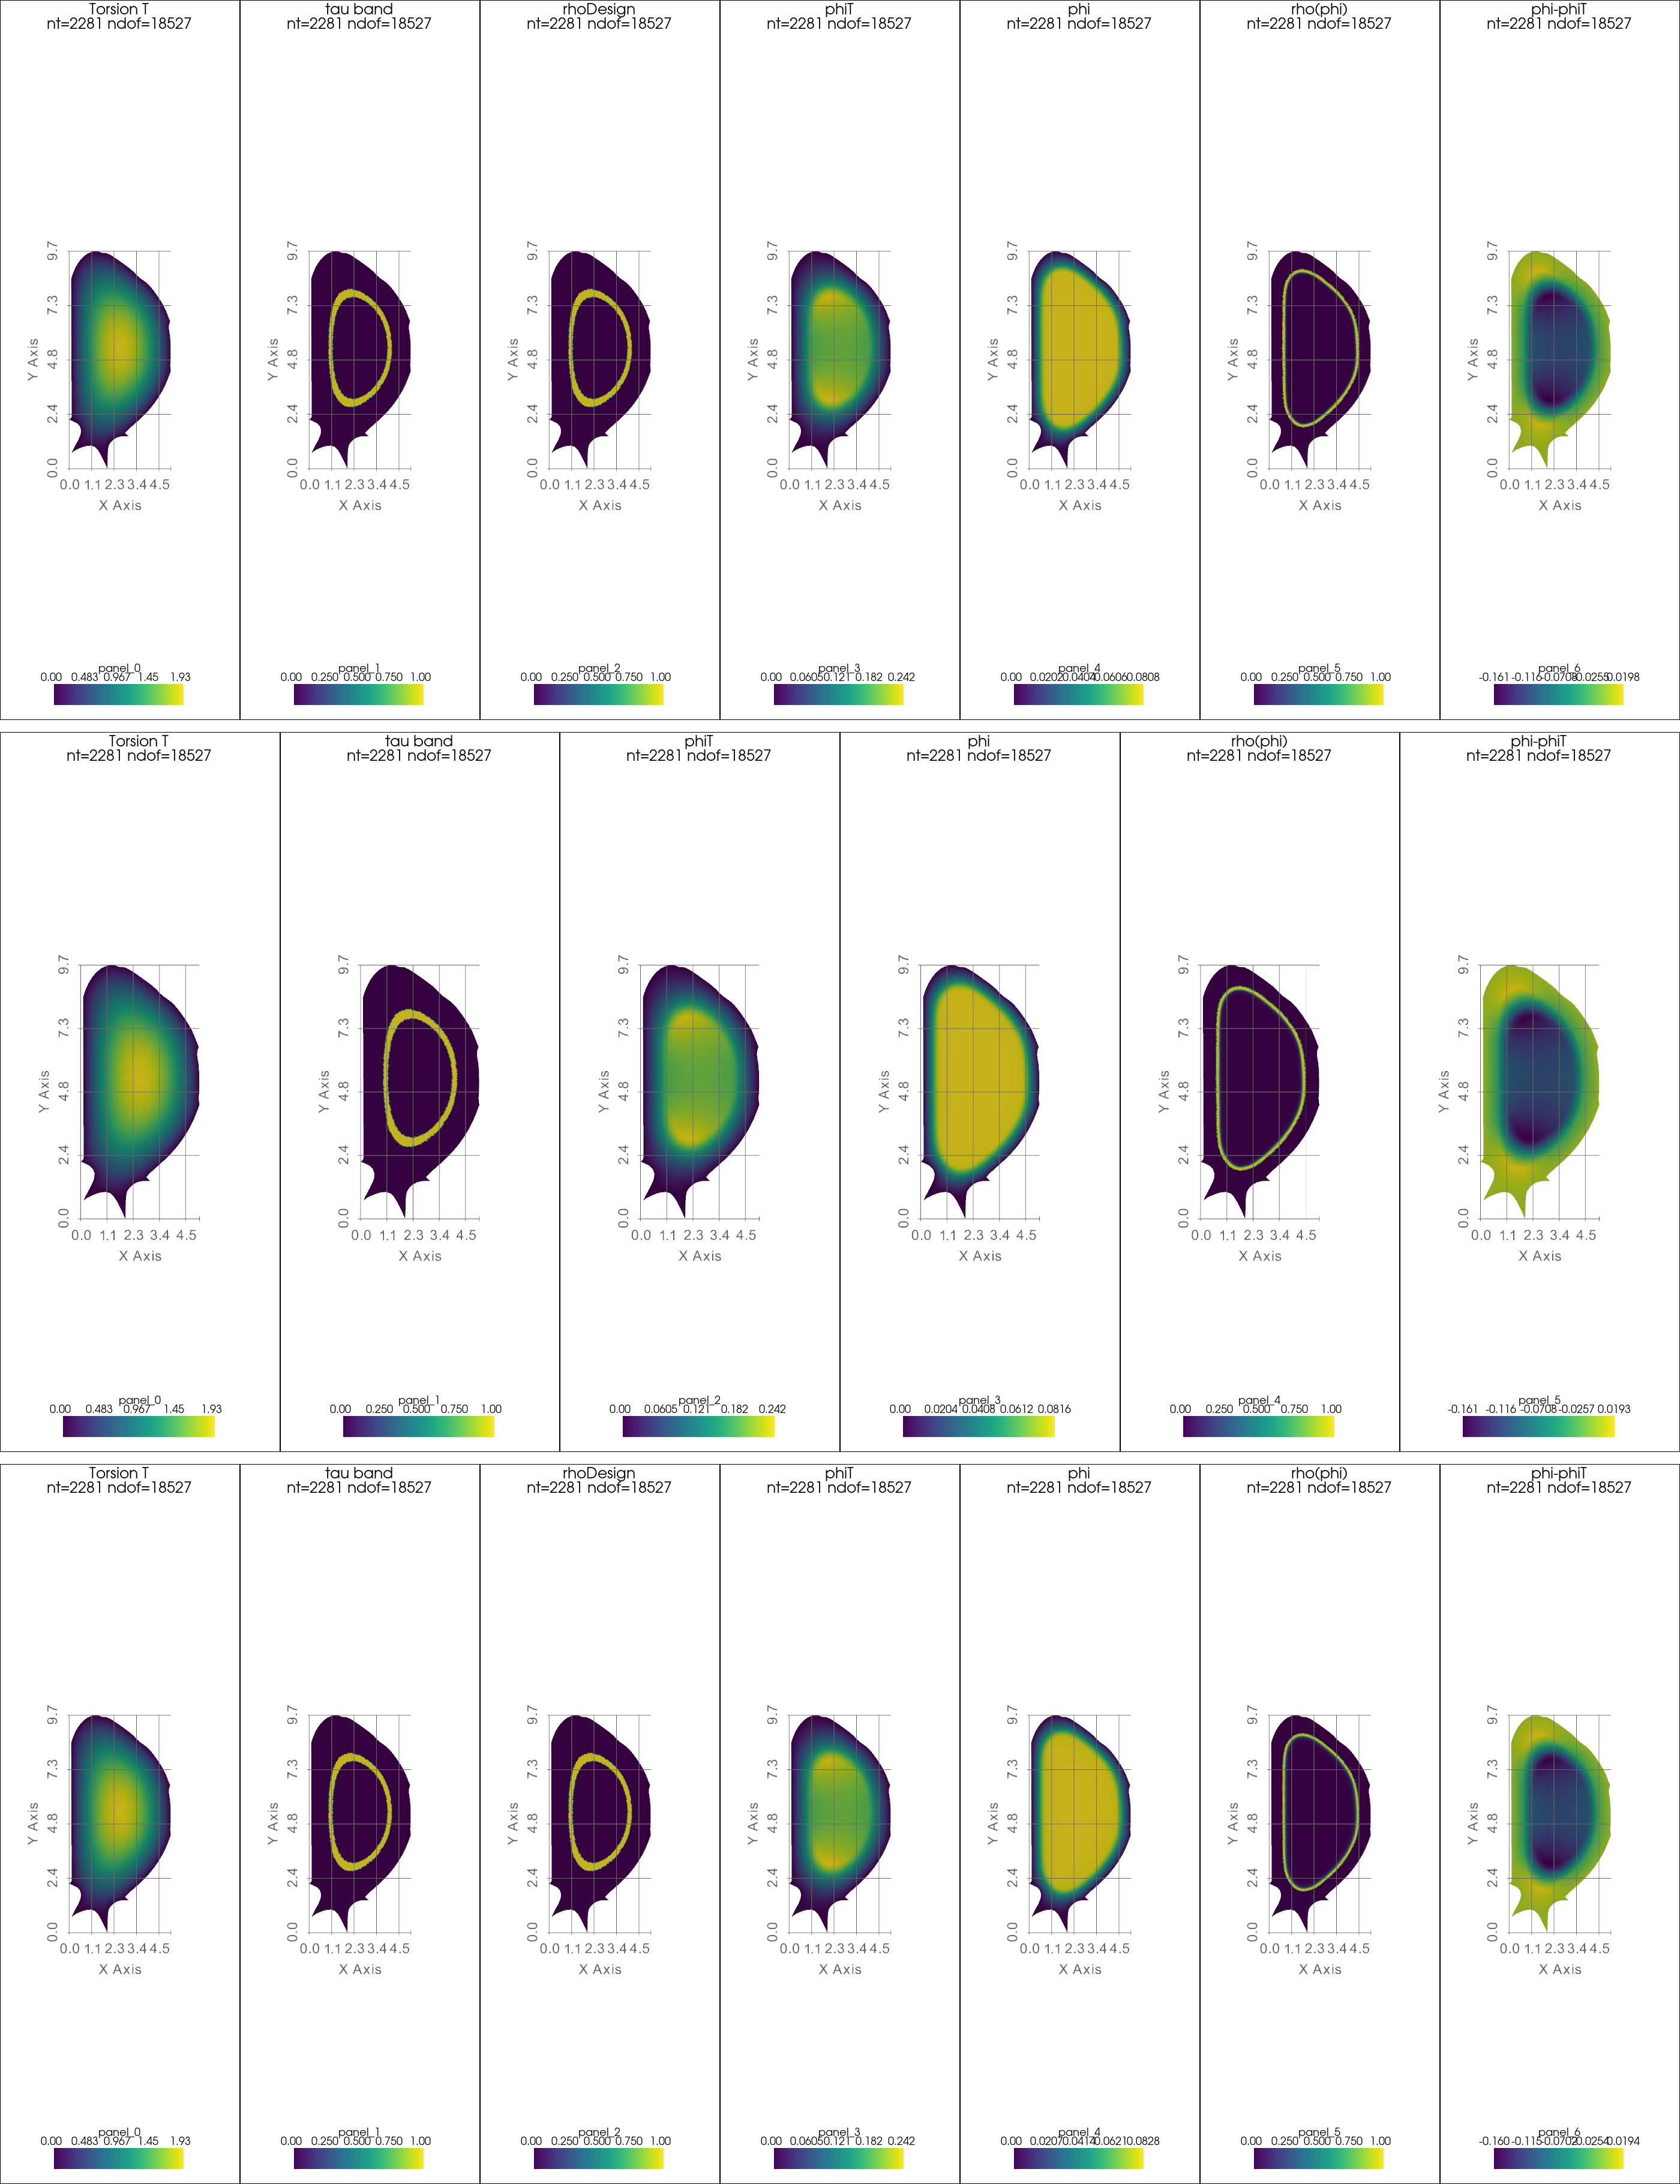
\includegraphics[width=0.88\linewidth,height=0.72\textheight,keepaspectratio]{figures/iter_0p6_0p7_bruteforce_active_eps002_lowdof_epsilon_fixed_pair_fields.png}
\caption{Full-field comparison for the matched threshold pair at smoothing ratios \(0.01\), \(0.02\), and \(0.04\).  Each constituent image is a complete rank-zero gather with hidden mesh edges.  The spatial branch remains displaced throughout the smoothing experiment.  Data status: actual.}
\label{fig:iter-active-epsilon-fields}
\end{figure}

\subsection{Adaptive level-curve search over the physical threshold triangle}
\label{sec:iter-adaptive-level-curve-search}

The static-grid diagnostic above establishes nonlinear feasibility but spends
many solves on bands which are already too thick or whose two equilibrium
level curves lie on the wrong torsion levels.  We therefore tested a successor
which uses no ITER-specific threshold cap: its loose domain is the complete
maximum-principle triangle
\[
 0\leq c_{1,\phi}<c_{2,\phi}\leq T_{\max}.
\]
Initial Chebyshev--Lobatto nodes cover this triangle.  Subsequent generations
bisect brackets selected from the signed lower- and upper-curve residuals.
Curve locations, spreads, containment, and orientation are measured by an
owned-cell coarea quadrature and fixed-bin MPI reductions.  The admissible
curve-position tolerances are computed from the current target field,
polynomial order, and local mesh resolution rather than from prior knowledge
of ITER.  If a solved pair is too thick, the fixed-\(c_1\) rule rejects all
larger \(c_2\), and the fixed-\(c_2\) rule rejects all smaller \(c_1\), provided
the observed branch retains the required monotone orientation.  In this first
implementation (v1), the \texttt{tooThick} flag was triggered by the robust
torsion-span test alone; the experiment below shows why that trigger must be
corroborated by a physical or hard-band thickness test before it is allowed to
prune.

The experiment uses the same inexpensive ITER control mesh as
Sec.~\ref{sec:iter-corrected-bruteforce}: \(2{,}281\) triangles,
\(18{,}527\) global P4 degrees of freedom, a discontinuous target band at
torsion fractions \([0.60,0.70]\), and
\(\varepsilon_\phi/(c_{2,\phi}-c_{1,\phi})=0.02\).  The candidate Newton
tolerance is \(10^{-6}\), with a 300-iteration cap.  A persistent 20-rank MPI
job forms twenty one-rank MUMPS candidate groups and assigns work through an
MPI-RMA fetch-and-add queue.  Across three nonempty generations it solved
\(37+97+6=140\) distinct pairs and retained 383 independently seeded Newton
branches; 24 additional points were rejected before solution by the
fixed-\(c_1\) thickness rule.  Of the solved pairs, 138 reached the candidate
Newton criterion, 34 possessed both active level curves, and 33 passed the
PDE/bound prefilter.  None passed either the practical geometric filter or
the stricter certification filter.  Consequently no reduced threshold
optimization was launched; this is a recorded initializer failure, not a
silently discarded run.

The diagnostic-best pair is
\[
 (c_{1,\phi},c_{2,\phi})=(0.2019124,0.2425665)
 =T_{\max}(0.1044041,0.1254253).
\]
It reaches residual \(1.02\times10^{-8}\), well below the search tolerance,
and both contours are active.  Its hard-band precision, recall, and Jaccard
index are \(0.61935\), \(0.73713\), and \(0.50730\), respectively.  This
apparently favorable area overlap is insufficient: the lower-curve
containment is only \(0.08222\), whereas the upper-curve containment is
\(0.97674\), and the robust torsion span \(0.17105\) exceeds its
resolution-aware limit \(0.14451\).  Hence v1 rejects the pair as both poorly
aligned and too thick.  The thickness conclusion is overconservative: its
hard-band torsion span is \(0.10315\), close to the target span \(0.1\), its
mean physical-thickness ratio is \(1.07568\), and the independent
\texttt{physicalTooThick} flag is false.  Candidate 107 therefore supplies
clear evidence of poor lower-curve alignment, but not of an unequivocally
over-wide physical band.  This discrepancy motivates the v2 rule, under which
robust-span excess can direct refinement but can prune a row or column only
when a hard-band or physical-thickness test corroborates it.

A second defect is visible at candidate 93.  Its generation-incumbent seed
converges to the zero branch with residual \(4.62\times10^{-16}\), but neither
threshold is active.  The torsion seed reaches residual
\(3.76\times10^{-7}\), has both thresholds active, satisfies the candidate PDE
filter, and has hard-band Jaccard index \(0.02044\).  Because both branches
have zero curve-fit score, v1 selects the inactive zero branch by its smaller
direct objective.  Branch selection must instead rank an active,
residual-qualified branch ahead of an inactive branch before comparing fit or
objective.  The v2 successor applies this ordering.  Finally, the
target-contour resolution test does not flag this mesh as underresolved, but
the low-resolution experiment remains a branch-discovery diagnostic and does
not prove non-attainability on finer meshes.

\begin{landscape}
\begin{figure}[tbp]
\centering
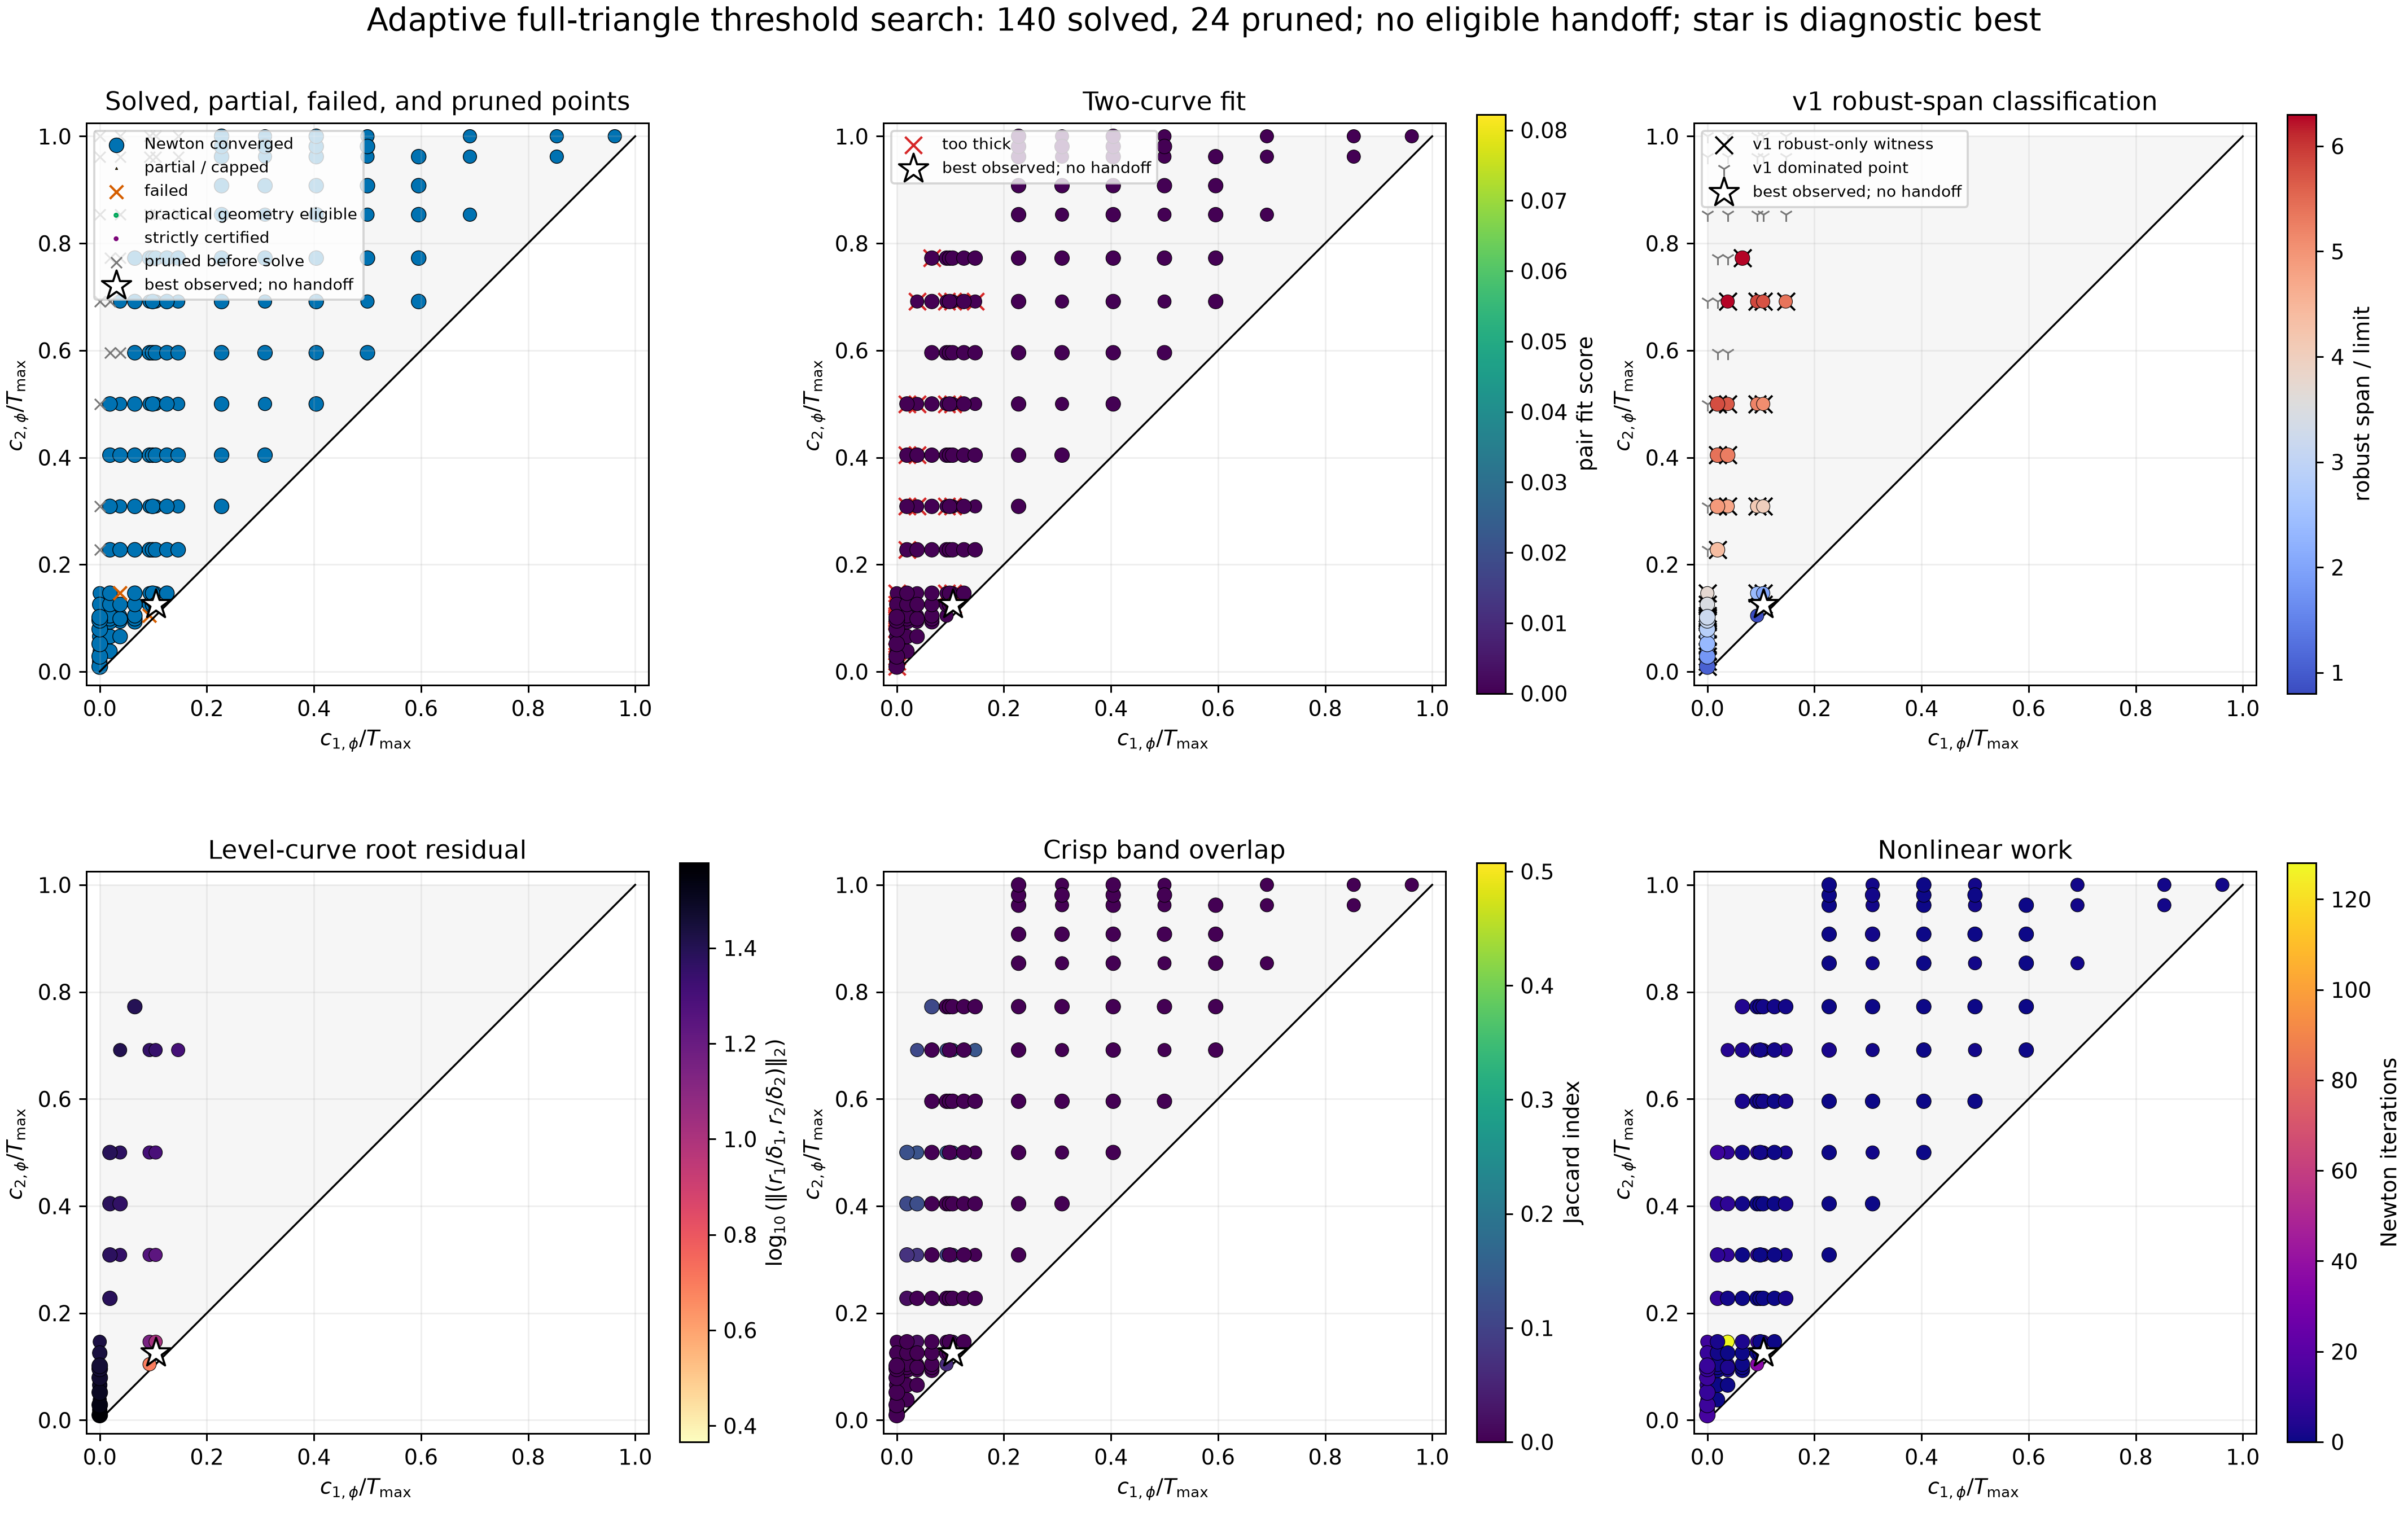
\includegraphics[width=0.92\linewidth,height=0.70\textheight,keepaspectratio]{figures/iter_0p6_0p7_adaptive_bisection_eps002_lowdof_search_summary.png}
\caption{Adaptive full-triangle search for ITER \([0.60,0.70]\).  All solved, partial, failed, and pre-solve-pruned points are retained.  The panels report nonlinear status, two-curve fit, the v1 robust-span thickness classification, normalized two-curve root residual, hard-band overlap, and Newton work.  The star is explicitly the best observed diagnostic pair, not an eligible optimizer handoff.  The robust-only thickness prunes are retained as v1 evidence but are not treated as physically certified.  Data status: actual; 140 solved pairs, 24 v1 dominance prunes, no geometrically eligible seed.}
\label{fig:iter-adaptive-search-summary}
\end{figure}
\end{landscape}

\begin{landscape}
\begin{figure}[tbp]
\centering
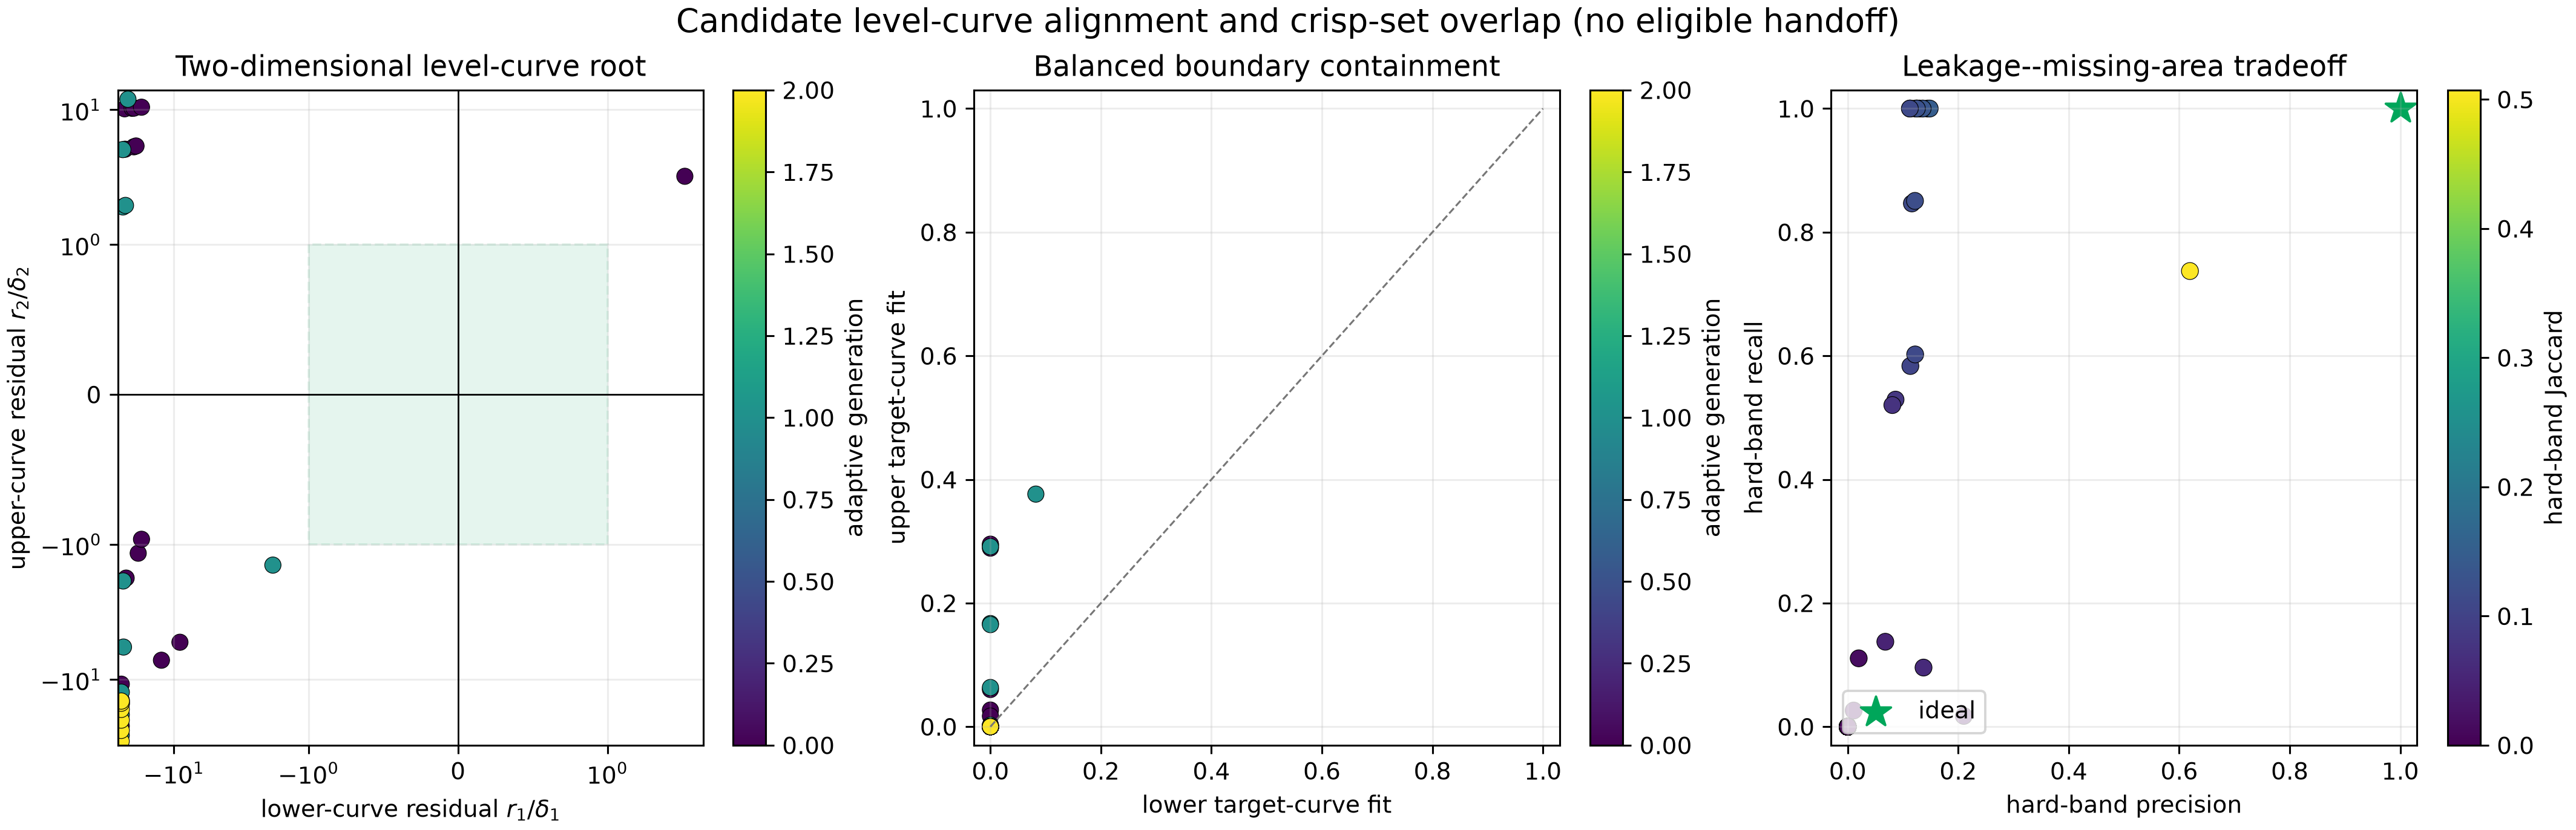
\includegraphics[width=0.97\linewidth]{figures/iter_0p6_0p7_adaptive_bisection_eps002_lowdof_curve_alignment.png}
\caption{Level-curve alignment audit.  The left panel treats candidate selection as a two-dimensional root problem in the lower- and upper-curve position residuals; the shaded box is the resolution-aware tolerance region.  The middle panel shows that no candidate simultaneously fits both target boundaries, and the right panel separates leakage (precision) from missing area (recall).  Data status: actual; unsuccessful candidates included.}
\label{fig:iter-adaptive-curve-alignment}
\end{figure}
\end{landscape}

\begin{landscape}
\begin{figure}[tbp]
\centering
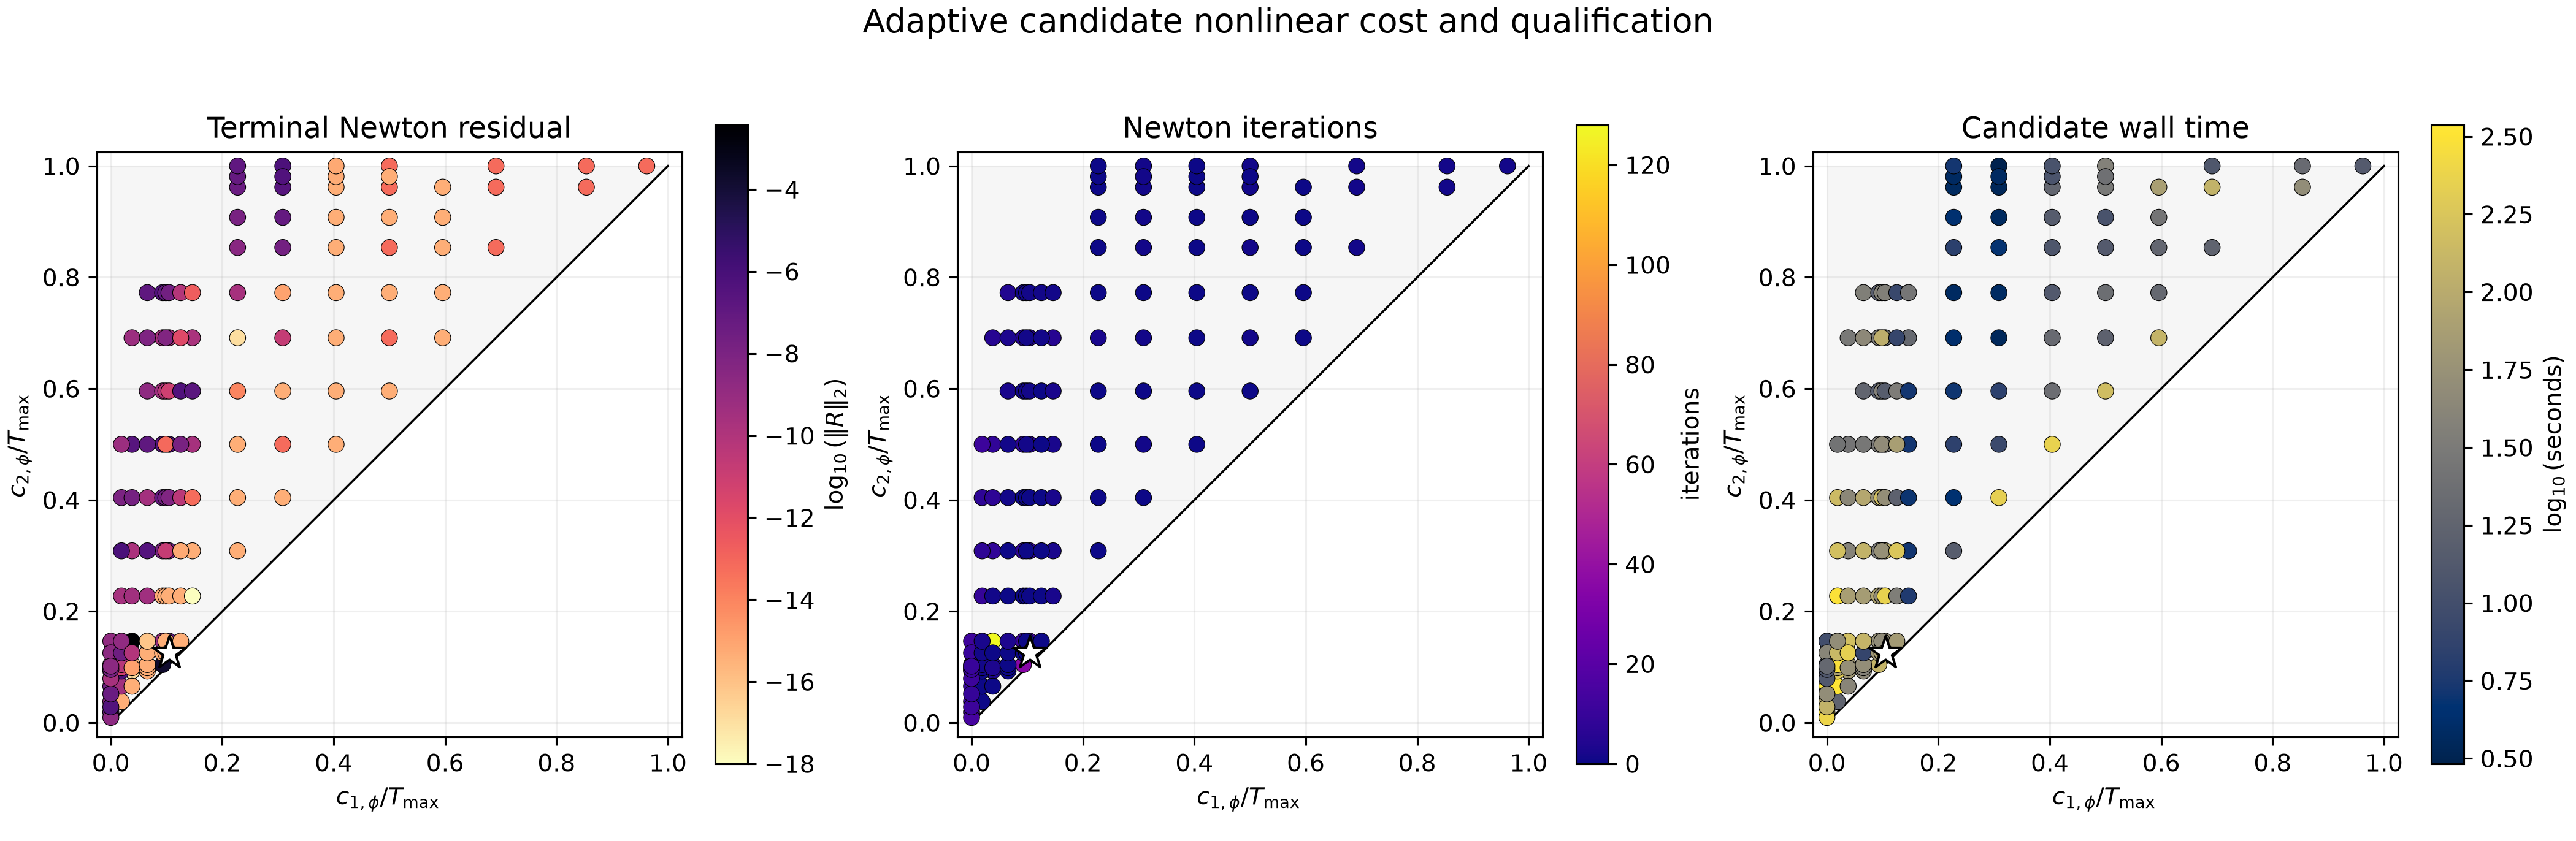
\includegraphics[width=0.97\linewidth]{figures/iter_0p6_0p7_adaptive_bisection_eps002_lowdof_newton_work.png}
\caption{Terminal residual, Newton iterations, and aggregate per-pair wall time over the normalized physical threshold triangle.  Immediate and partial branches are retained together with converged branches; the star again denotes only the diagnostic best.  Data status: actual; twenty concurrent one-rank MUMPS groups.}
\label{fig:iter-adaptive-newton-work}
\end{figure}
\end{landscape}

\begin{figure}[tbp]
\centering
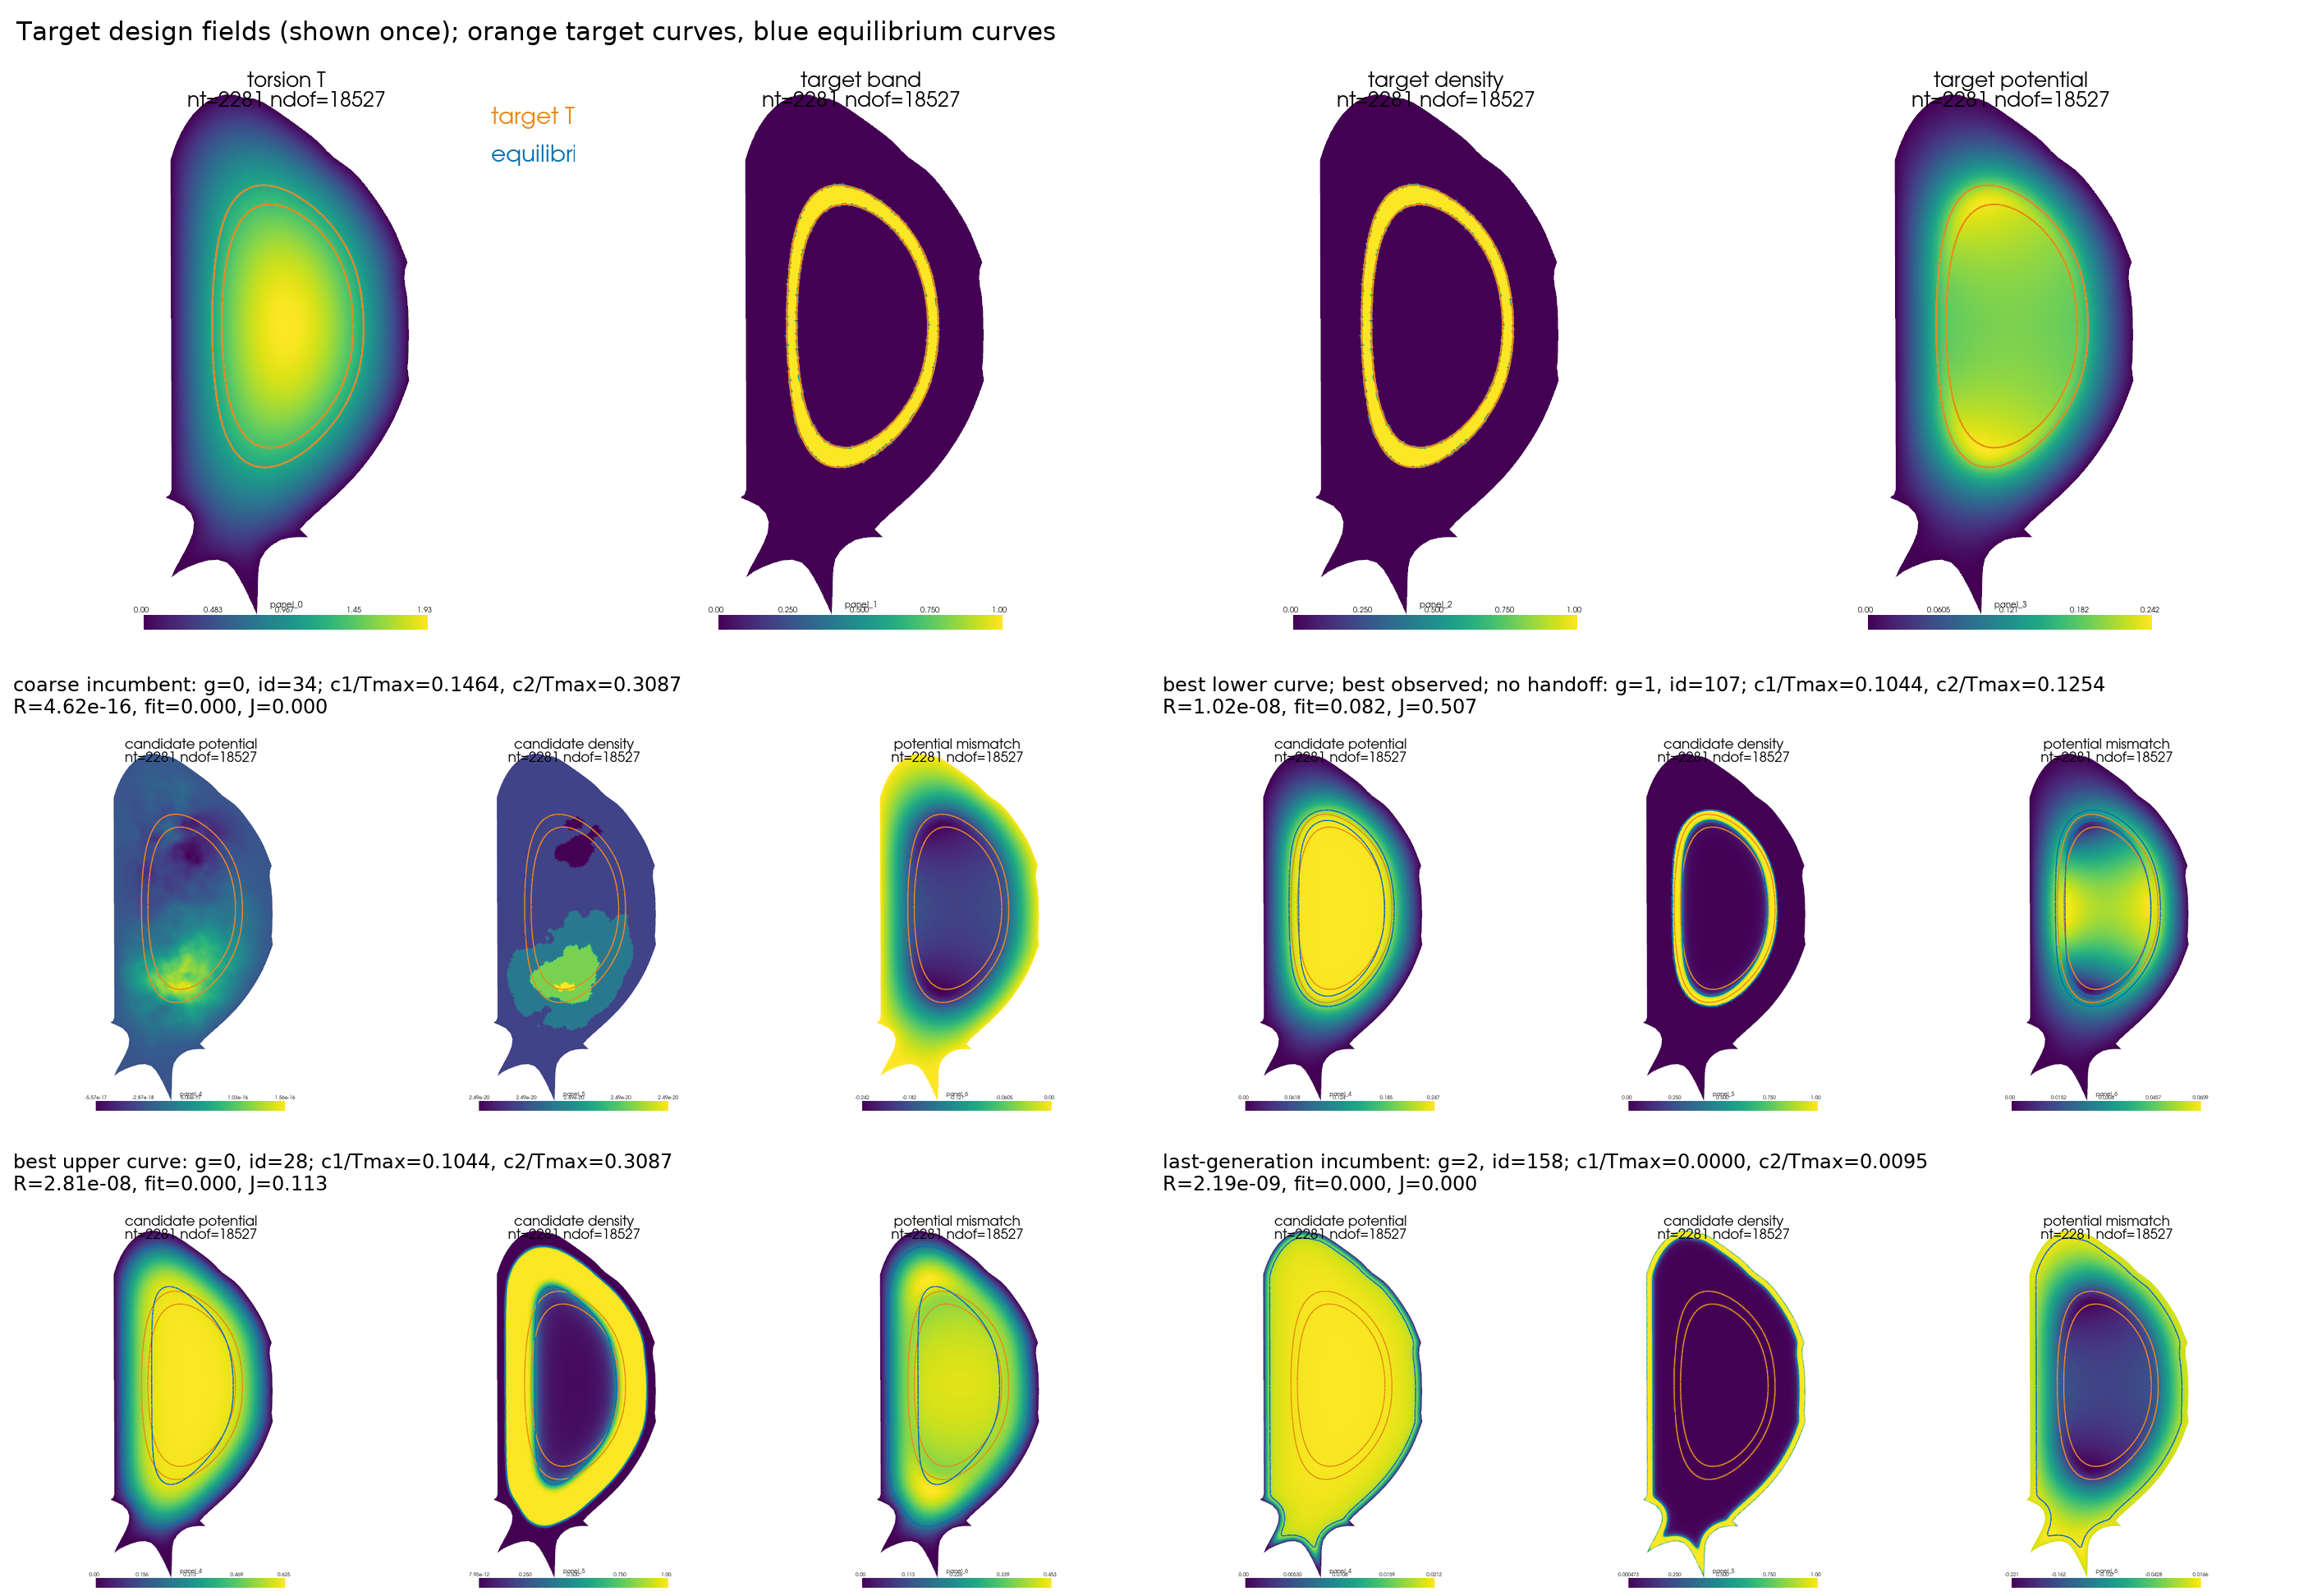
\includegraphics[width=0.96\linewidth,height=0.78\textheight,keepaspectratio]{figures/iter_0p6_0p7_adaptive_bisection_eps002_lowdof_candidate_storyboard.png}
\caption{Design-once adaptive-search storyboard.  The upper strip contains the four fixed design fields once; subsequent rows show candidate potential, density, and mismatch for the coarse incumbent, the best individual curve fits, the diagnostic-best pair, and the last-generation incumbent.  Every source is a complete rank-zero gather of all \(18{,}527\) P4 values with mesh edges suppressed.  No final optimizer panel is shown because no candidate satisfied the geometric handoff test.  Data status: actual; no-winner qualitative evidence.}
\label{fig:iter-adaptive-candidate-storyboard}
\end{figure}

All 140 solved candidate equilibria have an individual seven-panel,
lossless PNG.  The publication bundle also contains 35 four-candidate contact
sheets, so failure and partial convergence can be inspected without rerunning
the nonlinear solves.  Figures~\ref{fig:iter-adaptive-contact-early}--
\ref{fig:iter-adaptive-contact-late} retain three representative pages: the
broad search, the neighborhood containing candidate 107, and the transition
to the final adaptive generation.

\begin{landscape}
\begin{figure}[tbp]
\centering
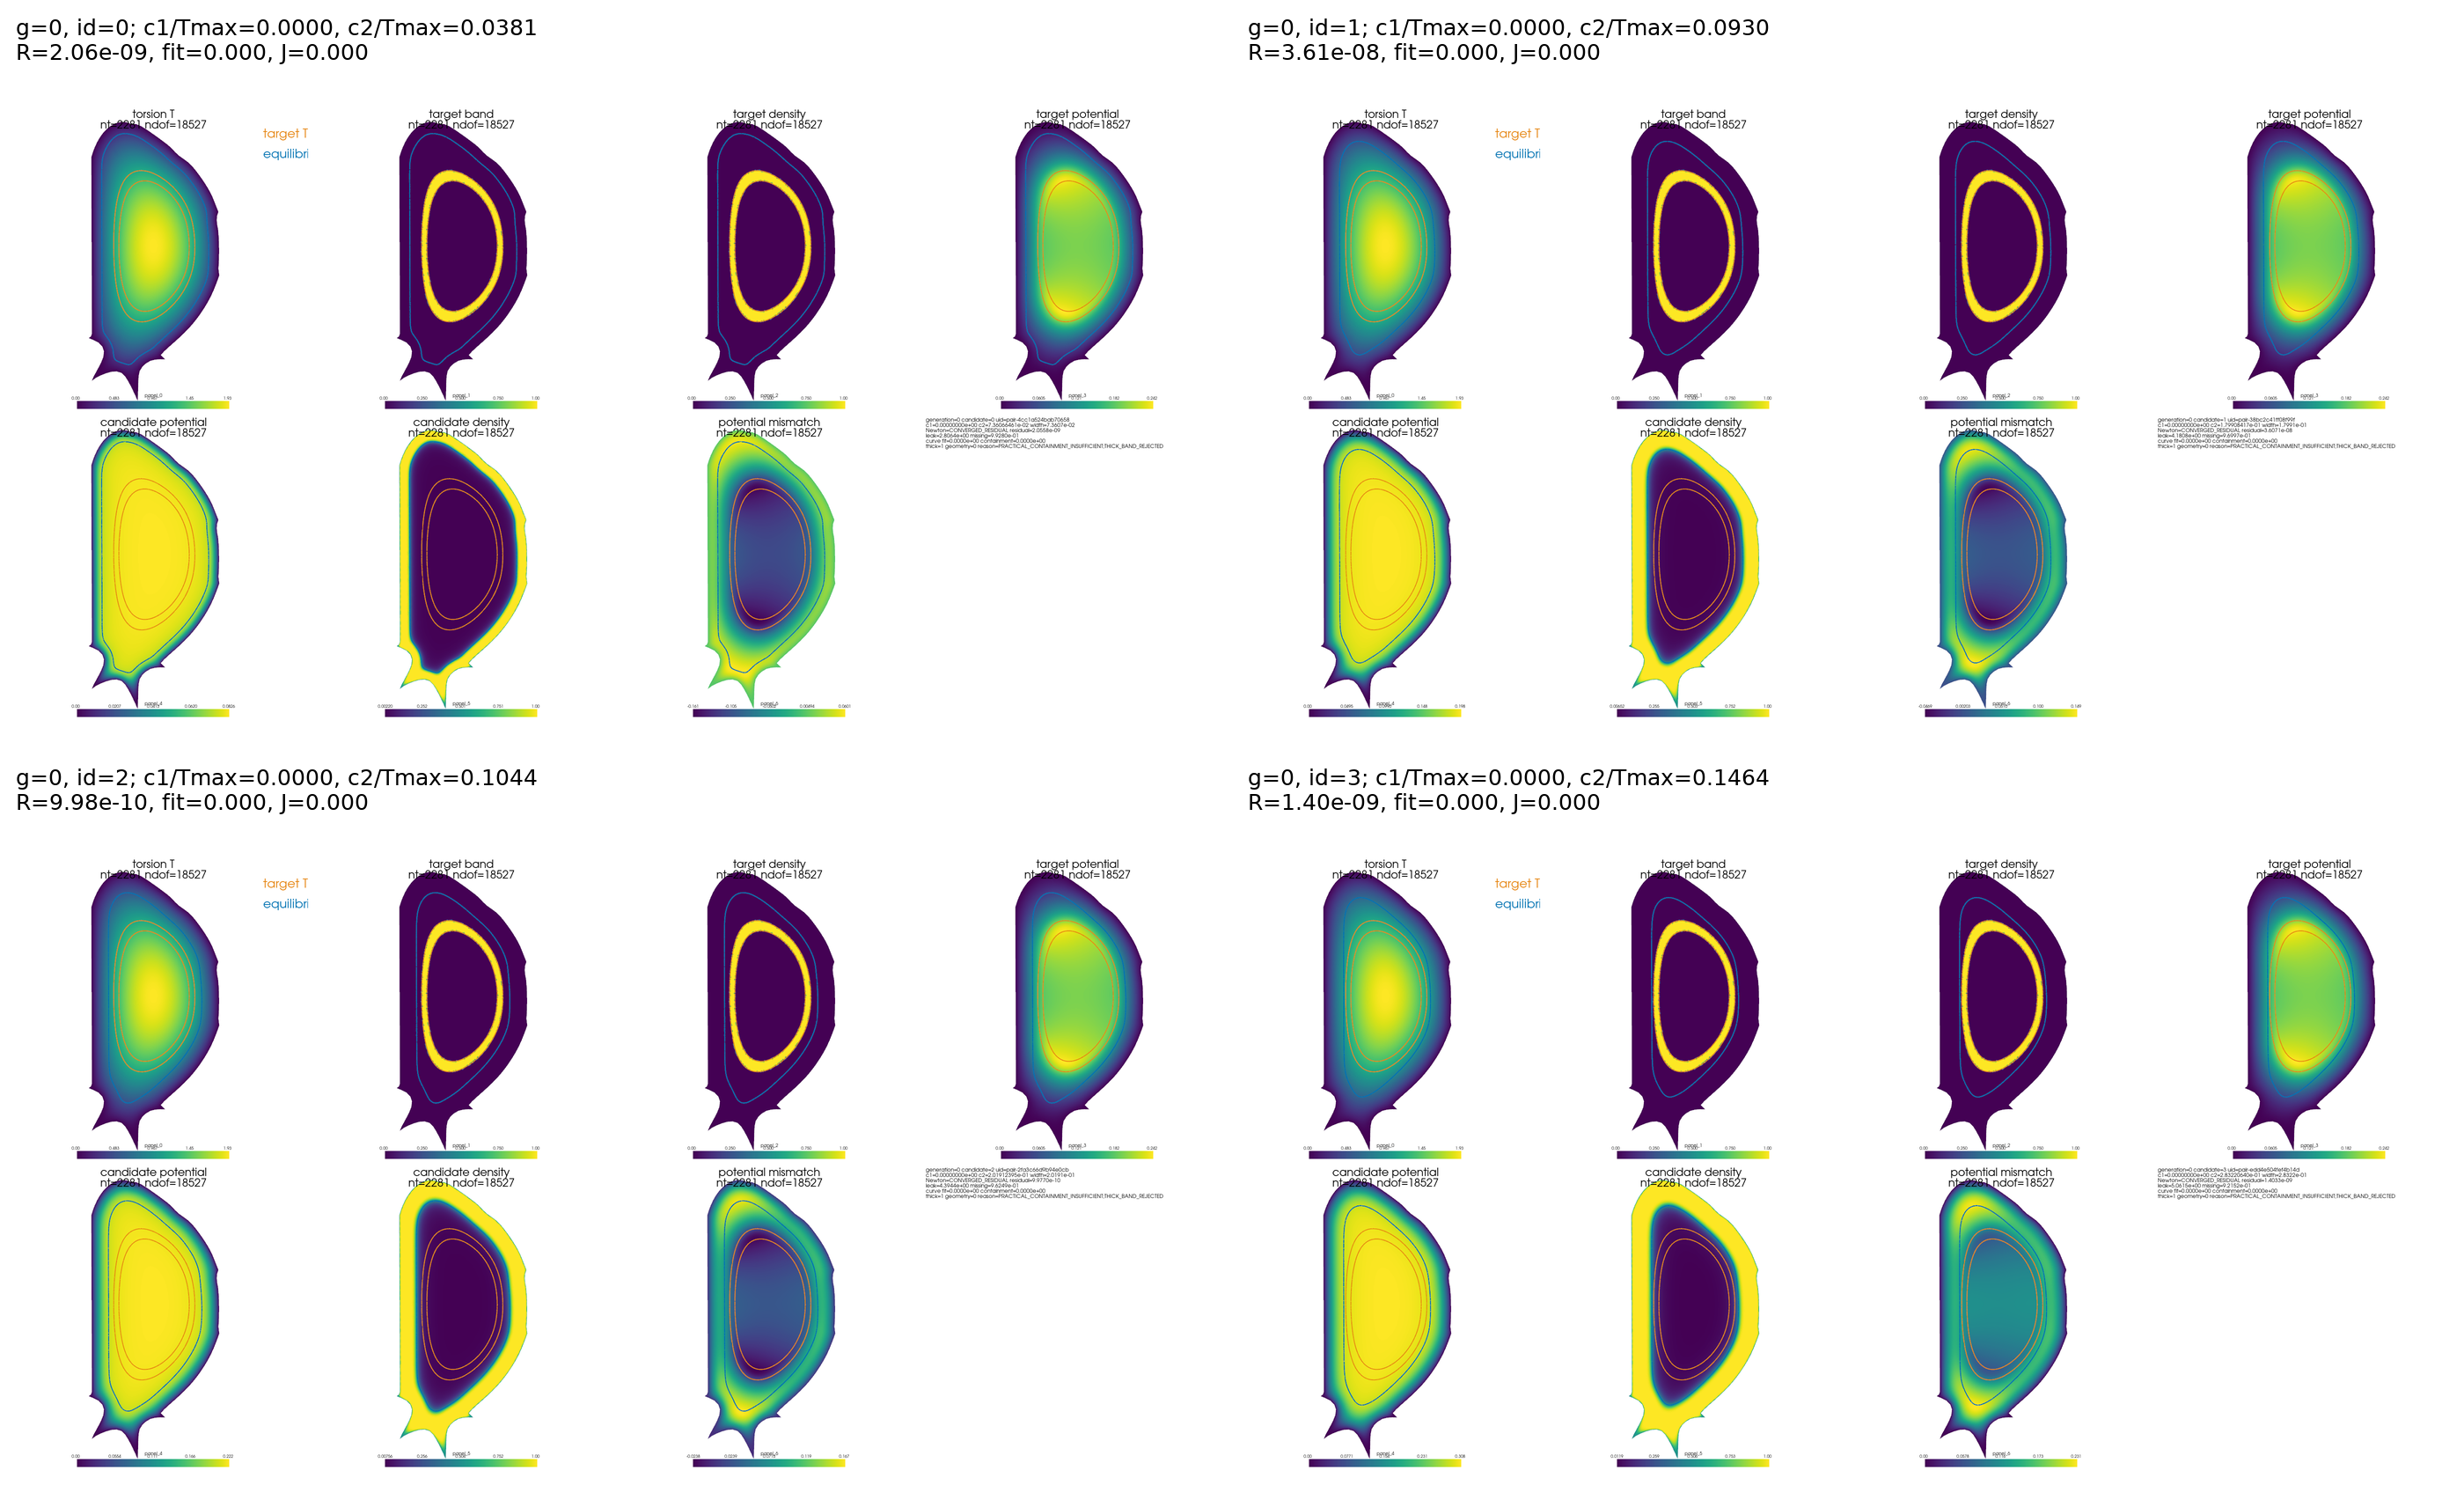
\includegraphics[width=0.97\linewidth]{figures/iter_0p6_0p7_adaptive_bisection_eps002_lowdof_candidate_contact_001.png}
\caption{First all-candidate contact page from the adaptive ITER archive.  Each tile contains torsion, target band, target density, target potential, candidate potential, candidate density, and mismatch.  Orange target and blue equilibrium contours are overlaid on complete fields, with no visible mesh.  Data status: actual; early broad-search candidates.}
\label{fig:iter-adaptive-contact-early}
\end{figure}
\end{landscape}

\begin{landscape}
\begin{figure}[tbp]
\centering
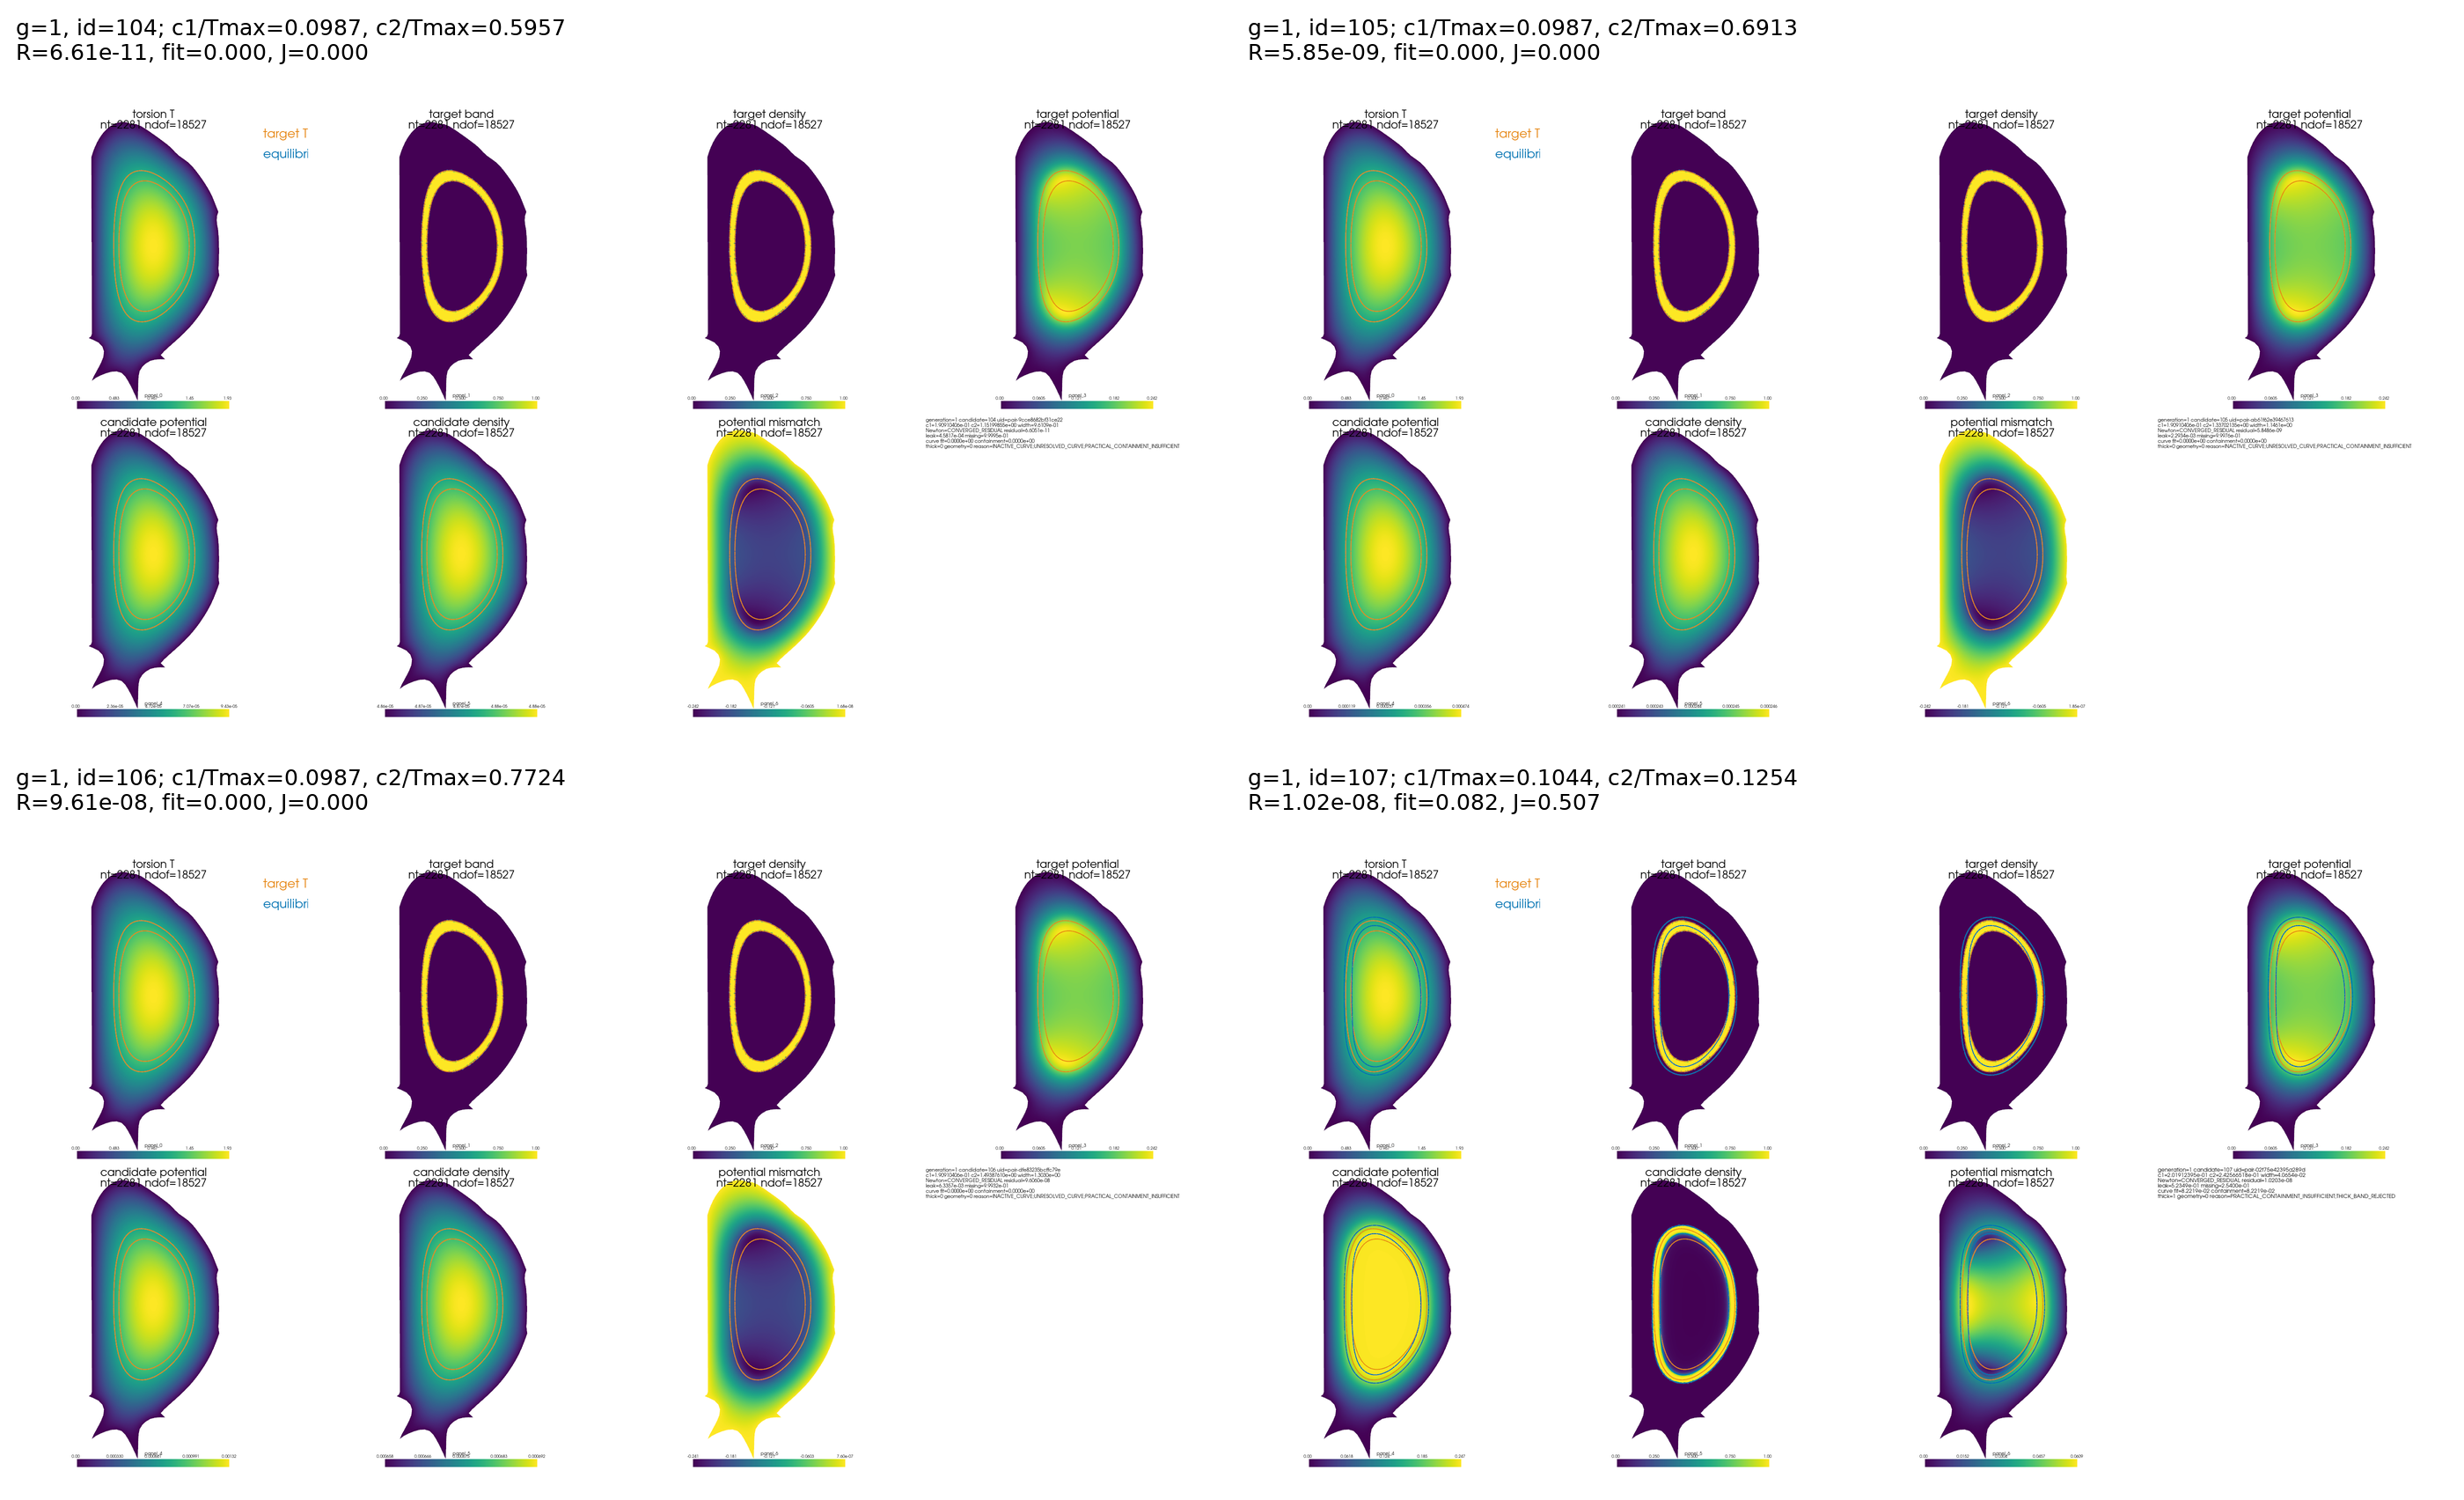
\includegraphics[width=0.97\linewidth]{figures/iter_0p6_0p7_adaptive_bisection_eps002_lowdof_candidate_contact_021.png}
\caption{Adaptive contact page containing the diagnostic-best candidate 107 (lower right).  Its equilibrium band visibly approaches the target annulus more closely than neighboring branches.  The lower-curve containment test correctly rejects the handoff, while comparison with the hard-band and physical-thickness measures shows that the additional v1 robust-only thickness label is overconservative.  Data status: actual; PDE-qualified geometric failure and algorithmic diagnostic retained.}
\label{fig:iter-adaptive-contact-best}
\end{figure}
\end{landscape}

\begin{landscape}
\begin{figure}[tbp]
\centering
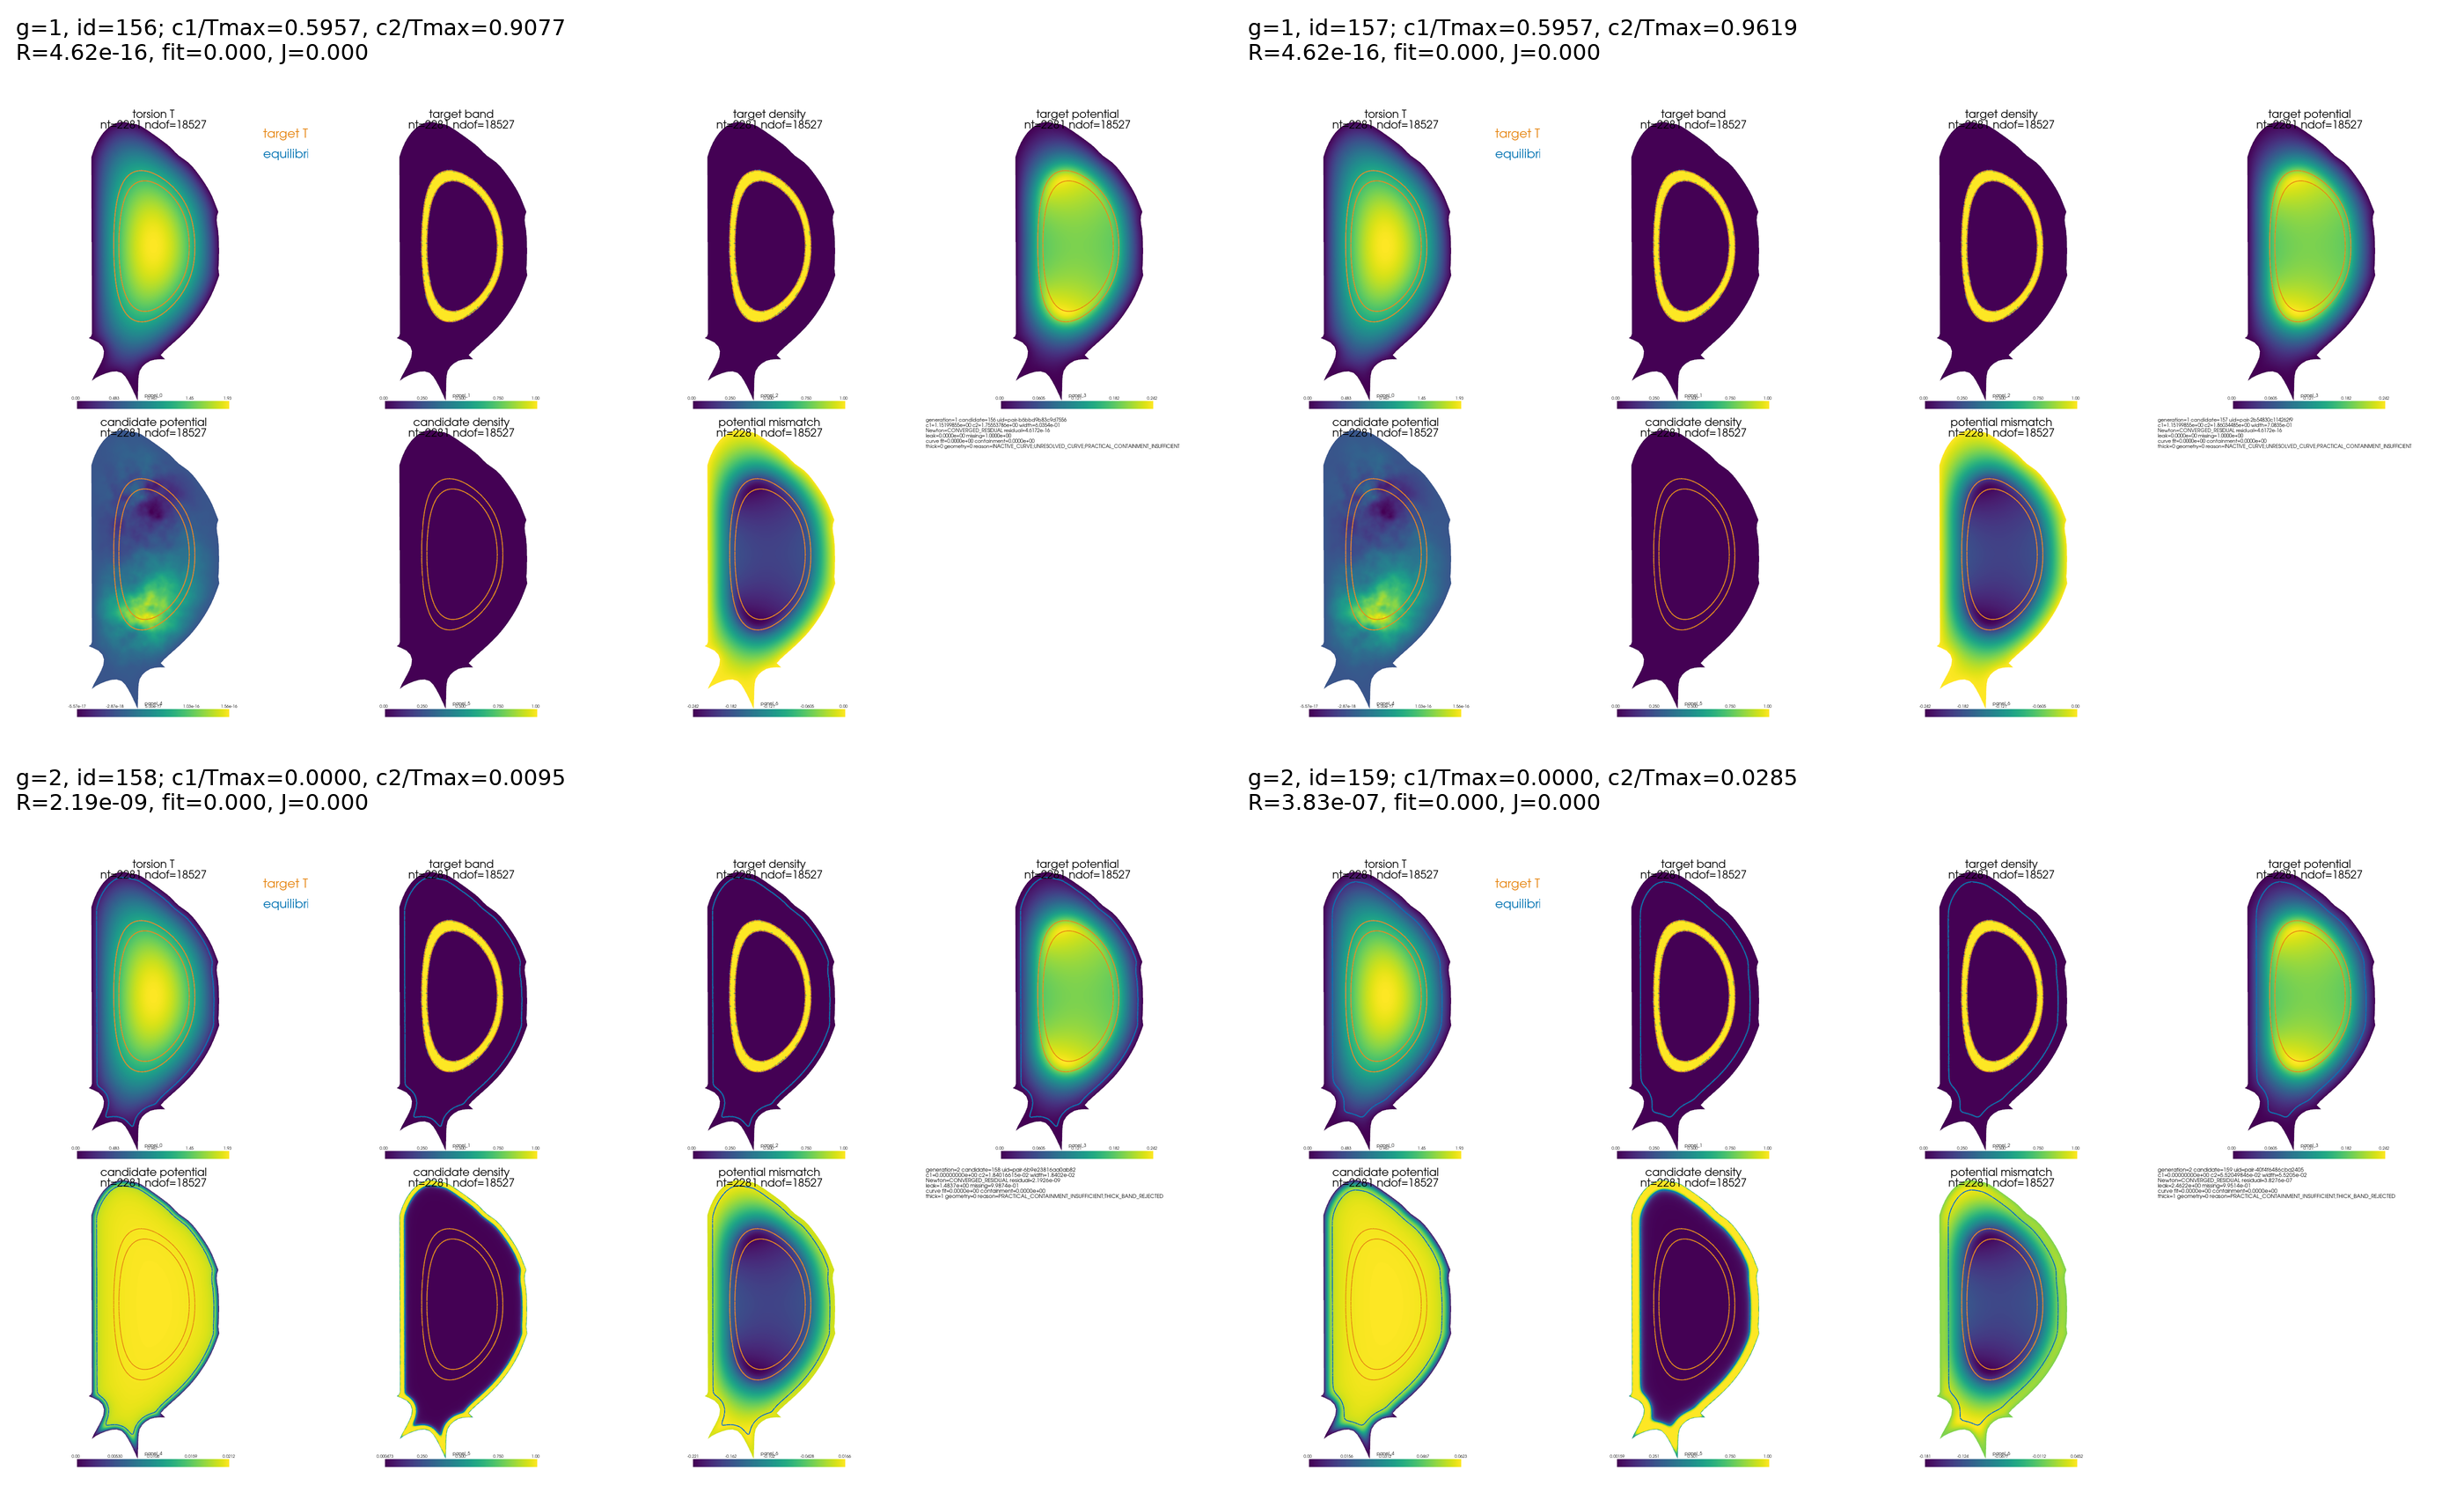
\includegraphics[width=0.97\linewidth]{figures/iter_0p6_0p7_adaptive_bisection_eps002_lowdof_candidate_contact_034.png}
\caption{Late adaptive contact page spanning the end of generation one and the first generation-two candidates.  These visually poor and partially degenerate equilibria remain in the archive and document where v1 refinement stopped; they do not certify that a corrected active-branch and corroborated-thickness search must stop at the same points.  Data status: actual; late unsuccessful candidates retained.}
\label{fig:iter-adaptive-contact-late}
\end{figure}
\end{landscape}

\paragraph{Continuation-aware v2 comparison.}
We repeated the same low-DOF ITER experiment after applying the two algorithmic
corrections identified by v1: an active, residual-qualified branch is preferred
to an inactive branch, and robust-span excess can prune only when the hard-band
span or physical-thickness test corroborates it.  The v2 search also propagates
nearby solved states between generations.  Seven initial nodes and five
adaptive generations produced \(30+22+4+4+4=64\) solved pairs; 14
fixed-\(c_1\) and 8 fixed-\(c_2\) dominance deductions pruned 22 additional
pairs before solution.  The same 20-rank MPI layout assigned these candidates
to twenty one-rank MUMPS groups.

Table~\ref{tab:iter-adaptive-v1-v2} shows a marked change in where the search
spends its nonlinear work.  The active-curve fraction rises from
\(34/140=24.3\%\) to \(52/64=81.3\%\), and the PDE/bound-qualified fraction
rises from \(33/140=23.6\%\) to \(43/64=67.2\%\).  Conversely, v2 deliberately
uses an 80-iteration initial candidate budget rather than the v1 cap of 300,
so its raw Newton-convergence fraction is lower.  These counts demonstrate
better branch targeting, but they are not an isolated timing comparison
because branch ordering, pruning, continuation, and the candidate budget all
changed simultaneously.

\begin{table}[tbp]
\centering
\caption{Observed v1--v2 adaptive-search outcomes on the same
\(18{,}527\)-DOF ITER discretization.  The geometry gate excludes the PDE
qualification; a handoff requires both.  Data status: actual.}
\label{tab:iter-adaptive-v1-v2}
\begin{tabular}{lrr}
\toprule
Outcome & v1 & continuation-aware v2 \\
\midrule
Solved candidate pairs & 140 & 64 \\
Pre-solve dominance prunes & 24 & 22 \\
Newton-converged pairs & 138 (98.6\%) & 53 (82.8\%) \\
Pairs with both curves active & 34 (24.3\%) & 52 (81.3\%) \\
PDE/bound-qualified pairs & 33 (23.6\%) & 43 (67.2\%) \\
Geometry-gate passes & 0 & 1 \\
Complete optimizer handoffs & 0 & 0 \\
\bottomrule
\end{tabular}
\end{table}

Candidate 80 explains why the PDE and geometric gates must remain separate.
At normalized thresholds \(c_{1,\phi}/T_{\max}=0.0800068\) and
\(c_{2,\phi}/T_{\max}=0.0897715\), it has hard-band Jaccard index \(0.67671\),
containment \(0.94136\), paired
curve-fit score \(0.59249\), normalized curve error \(0.85057\), and no robust,
hard-span, or physical-thickness warning.  It therefore passes the geometric
gate.  Its nonlinear solve, however, terminates with
\texttt{FAIL\_LS} at residual \(2.628\times10^{-3}\); it is not PDE-qualified
and is not handed to the reduced optimizer.  This is direct numerical evidence
for retaining a residual gate before reusing a Newton matrix for threshold
sensitivities: a visually and geometrically favorable intermediate state is
not by itself a valid stationary branch.

Candidate 84 is the best PDE-qualified diagnostic pair.  At normalized
thresholds \(c_{1,\phi}/T_{\max}=0.0800068\) and
\(c_{2,\phi}/T_{\max}=0.0913989\), it reaches residual
\(2.194\times10^{-7}\), below the \(10^{-6}\) search
criterion, with Jaccard index \(0.47302\), containment \(0.41594\), and no
thickness warning.  Nevertheless, its normalized upper-curve position error
is \(2.337\), exceeding the handoff cap of \(2\).  It is therefore rejected
geometrically.  The recorded status remains
\texttt{NO\_HANDOFF\_ELIGIBLE\_SEED}; neither candidate is an optimizer
success.

The candidate Newton policy used an initial budget of 80 iterations, a
20-iteration extension chunk, contraction threshold \(0.98\), and hard ceiling
800.  Among 136 branch trials, 12 reached the initial cap and every one was
classified as weakly contracting.  Consequently the soft-cap policy made zero
extensions.  For this run, the continuation rule avoided spending additional
iterations on the observed stalled branches; this single experiment does not
establish that the same contraction threshold is optimal on other geometries
or resolutions.

\begin{landscape}
\begin{figure}[tbp]
\centering
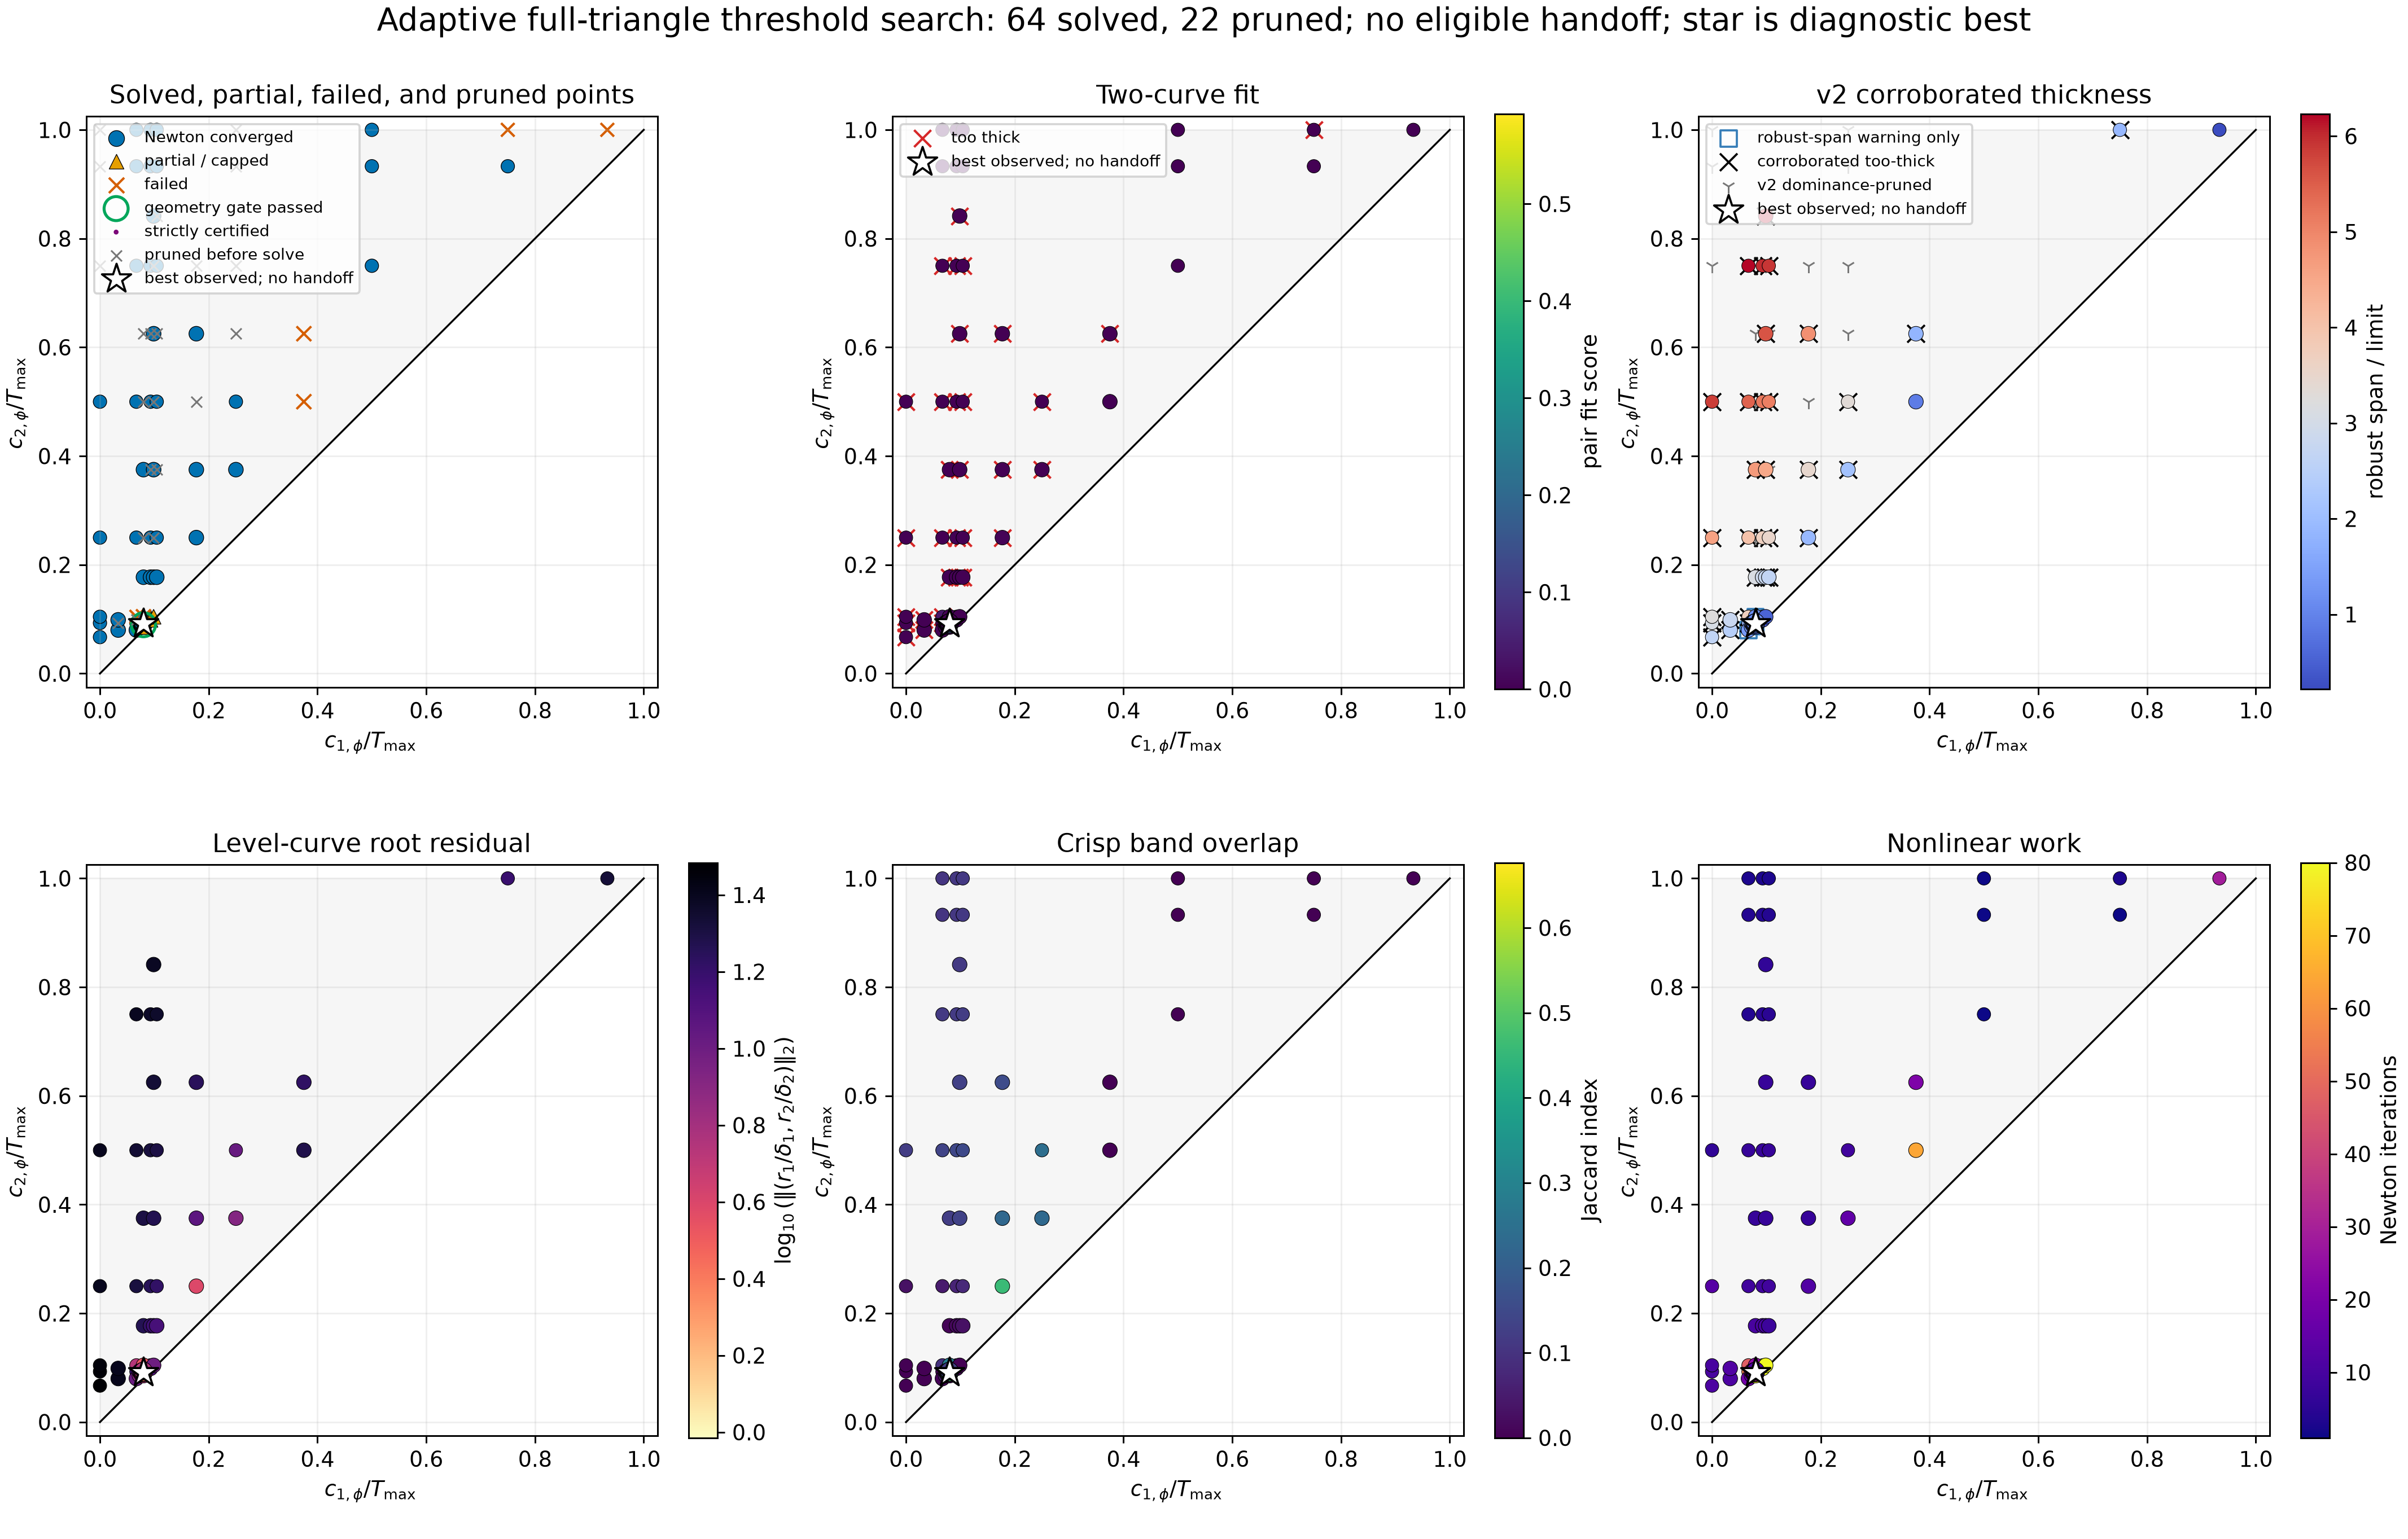
\includegraphics[width=0.92\linewidth,height=0.70\textheight,keepaspectratio]{figures/iter_0p6_0p7_adaptive_continuation_eps002_lowdof_search_summary.png}
\caption{Continuation-aware v2 search over the full physical threshold
triangle.  The six panels retain nonlinear failures and pre-solve prunes,
two-curve fit, the corrected corroborated-thickness decision, normalized
curve error, hard-band overlap, and Newton work.  Open blue squares in the
thickness panel denote a robust-span warning without corroboration; black
crosses denote corroborated rejection.  The green ring identifies the sole
geometry-gate pass, candidate 80, while the star is the PDE-qualified
diagnostic best, candidate 84.  Neither is a complete handoff.  Data status:
actual; 64 solved pairs and 22 prunes.}
\label{fig:iter-adaptive-v2-search-summary}
\end{figure}
\end{landscape}

\begin{landscape}
\begin{figure}[tbp]
\centering
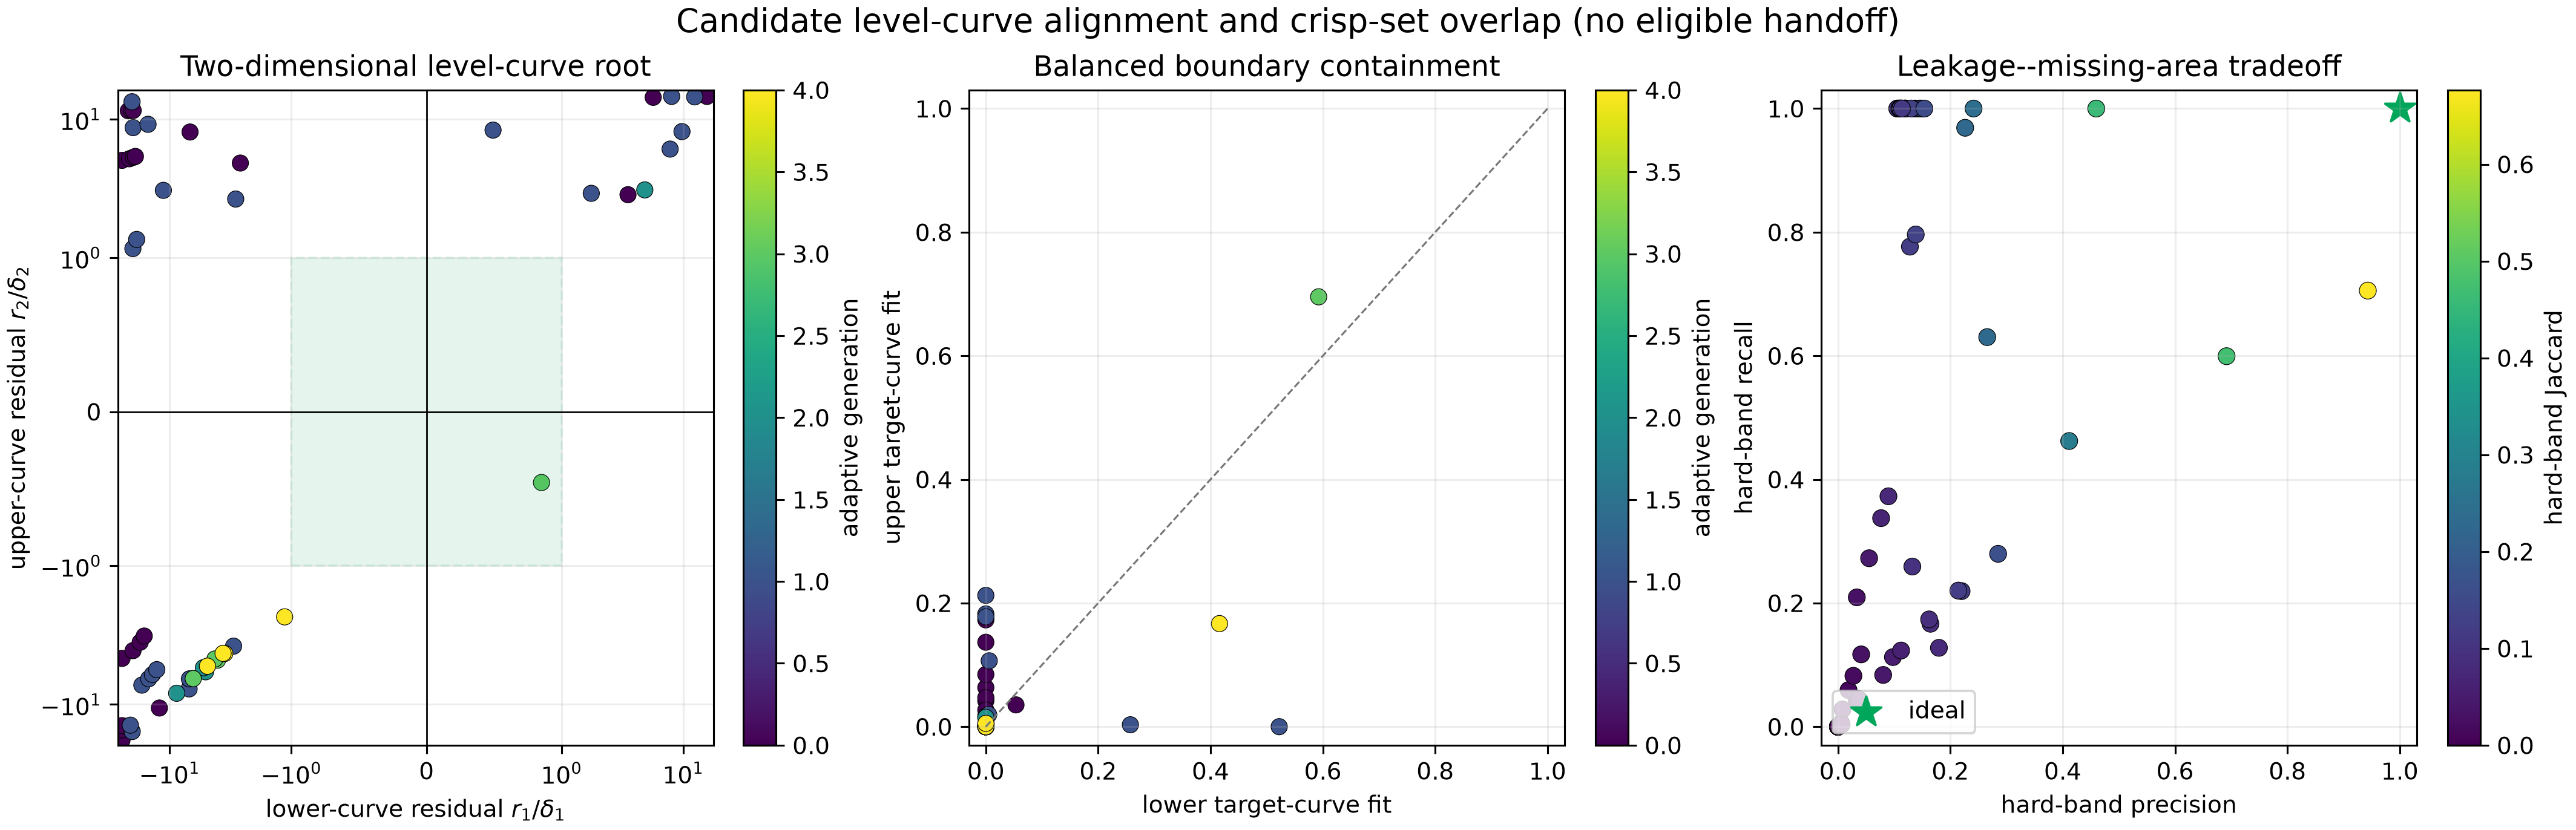
\includegraphics[width=0.94\linewidth,height=0.70\textheight,keepaspectratio]{figures/iter_0p6_0p7_adaptive_continuation_eps002_lowdof_curve_alignment.png}
\caption{v2 curve-alignment diagnostics: normalized lower/upper root
residuals, balanced boundary containment, and the precision--recall tradeoff.
The corrected branch preference populates the active two-curve region much
more densely than v1.  Candidate 80 reaches the geometric gate but lacks a
converged PDE state; candidate 84 is PDE-qualified but lies beyond the
upper-curve handoff tolerance.  Data status: actual; unsuccessful candidates
retained.}
\label{fig:iter-adaptive-v2-curve-alignment}
\end{figure}
\end{landscape}

\begin{landscape}
\begin{figure}[tbp]
\centering
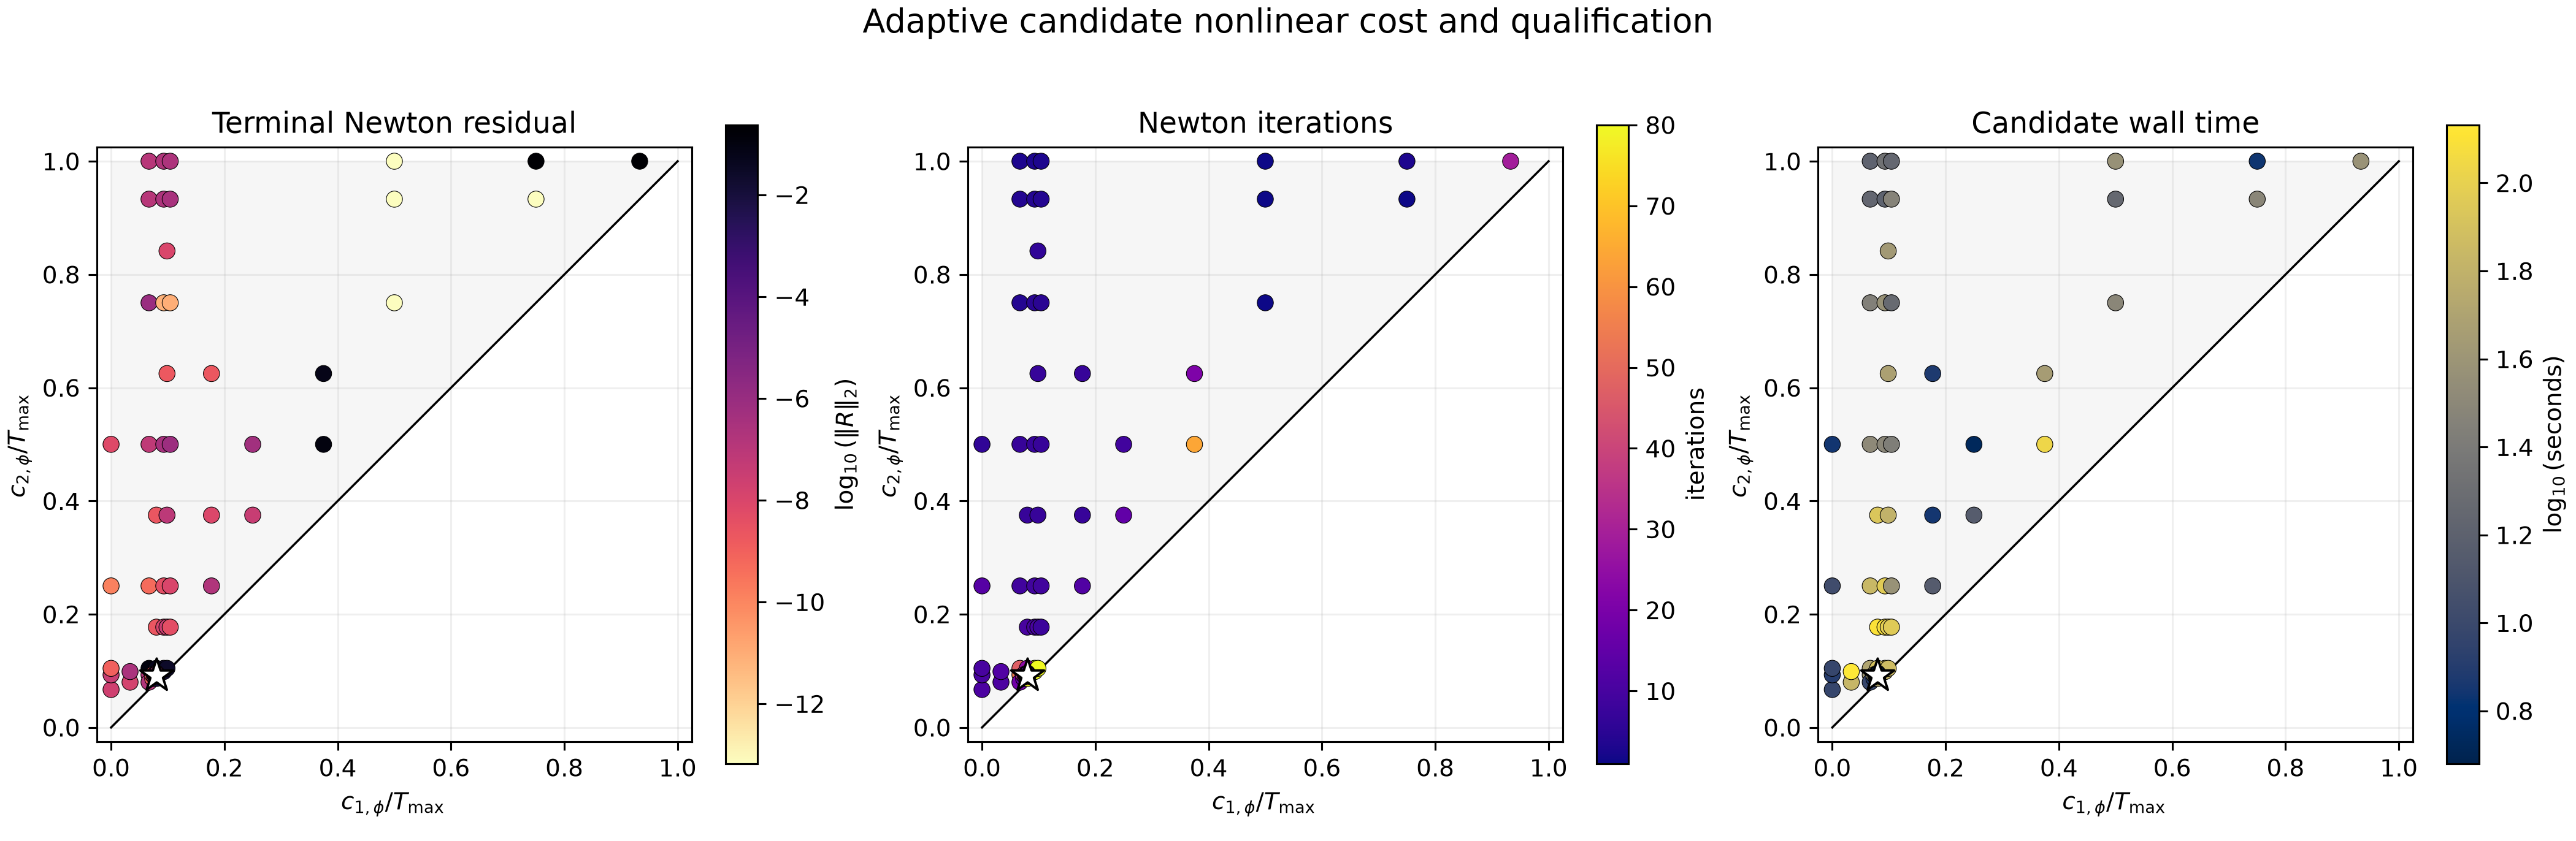
\includegraphics[width=0.94\linewidth,height=0.70\textheight,keepaspectratio]{figures/iter_0p6_0p7_adaptive_continuation_eps002_lowdof_newton_work.png}
\caption{v2 terminal Newton residual, iterations, and aggregate candidate wall
time.  The 80-iteration ceiling visible in the middle panel is the initial
soft cap; the branch-trial log records 12 cap hits, all stopped for weak
contraction and none extended.  The star denotes candidate 84 as a diagnostic
best, not an eligible optimizer handoff.  Data status: actual.}
\label{fig:iter-adaptive-v2-newton-work}
\end{figure}
\end{landscape}

\begin{figure}[tbp]
\centering
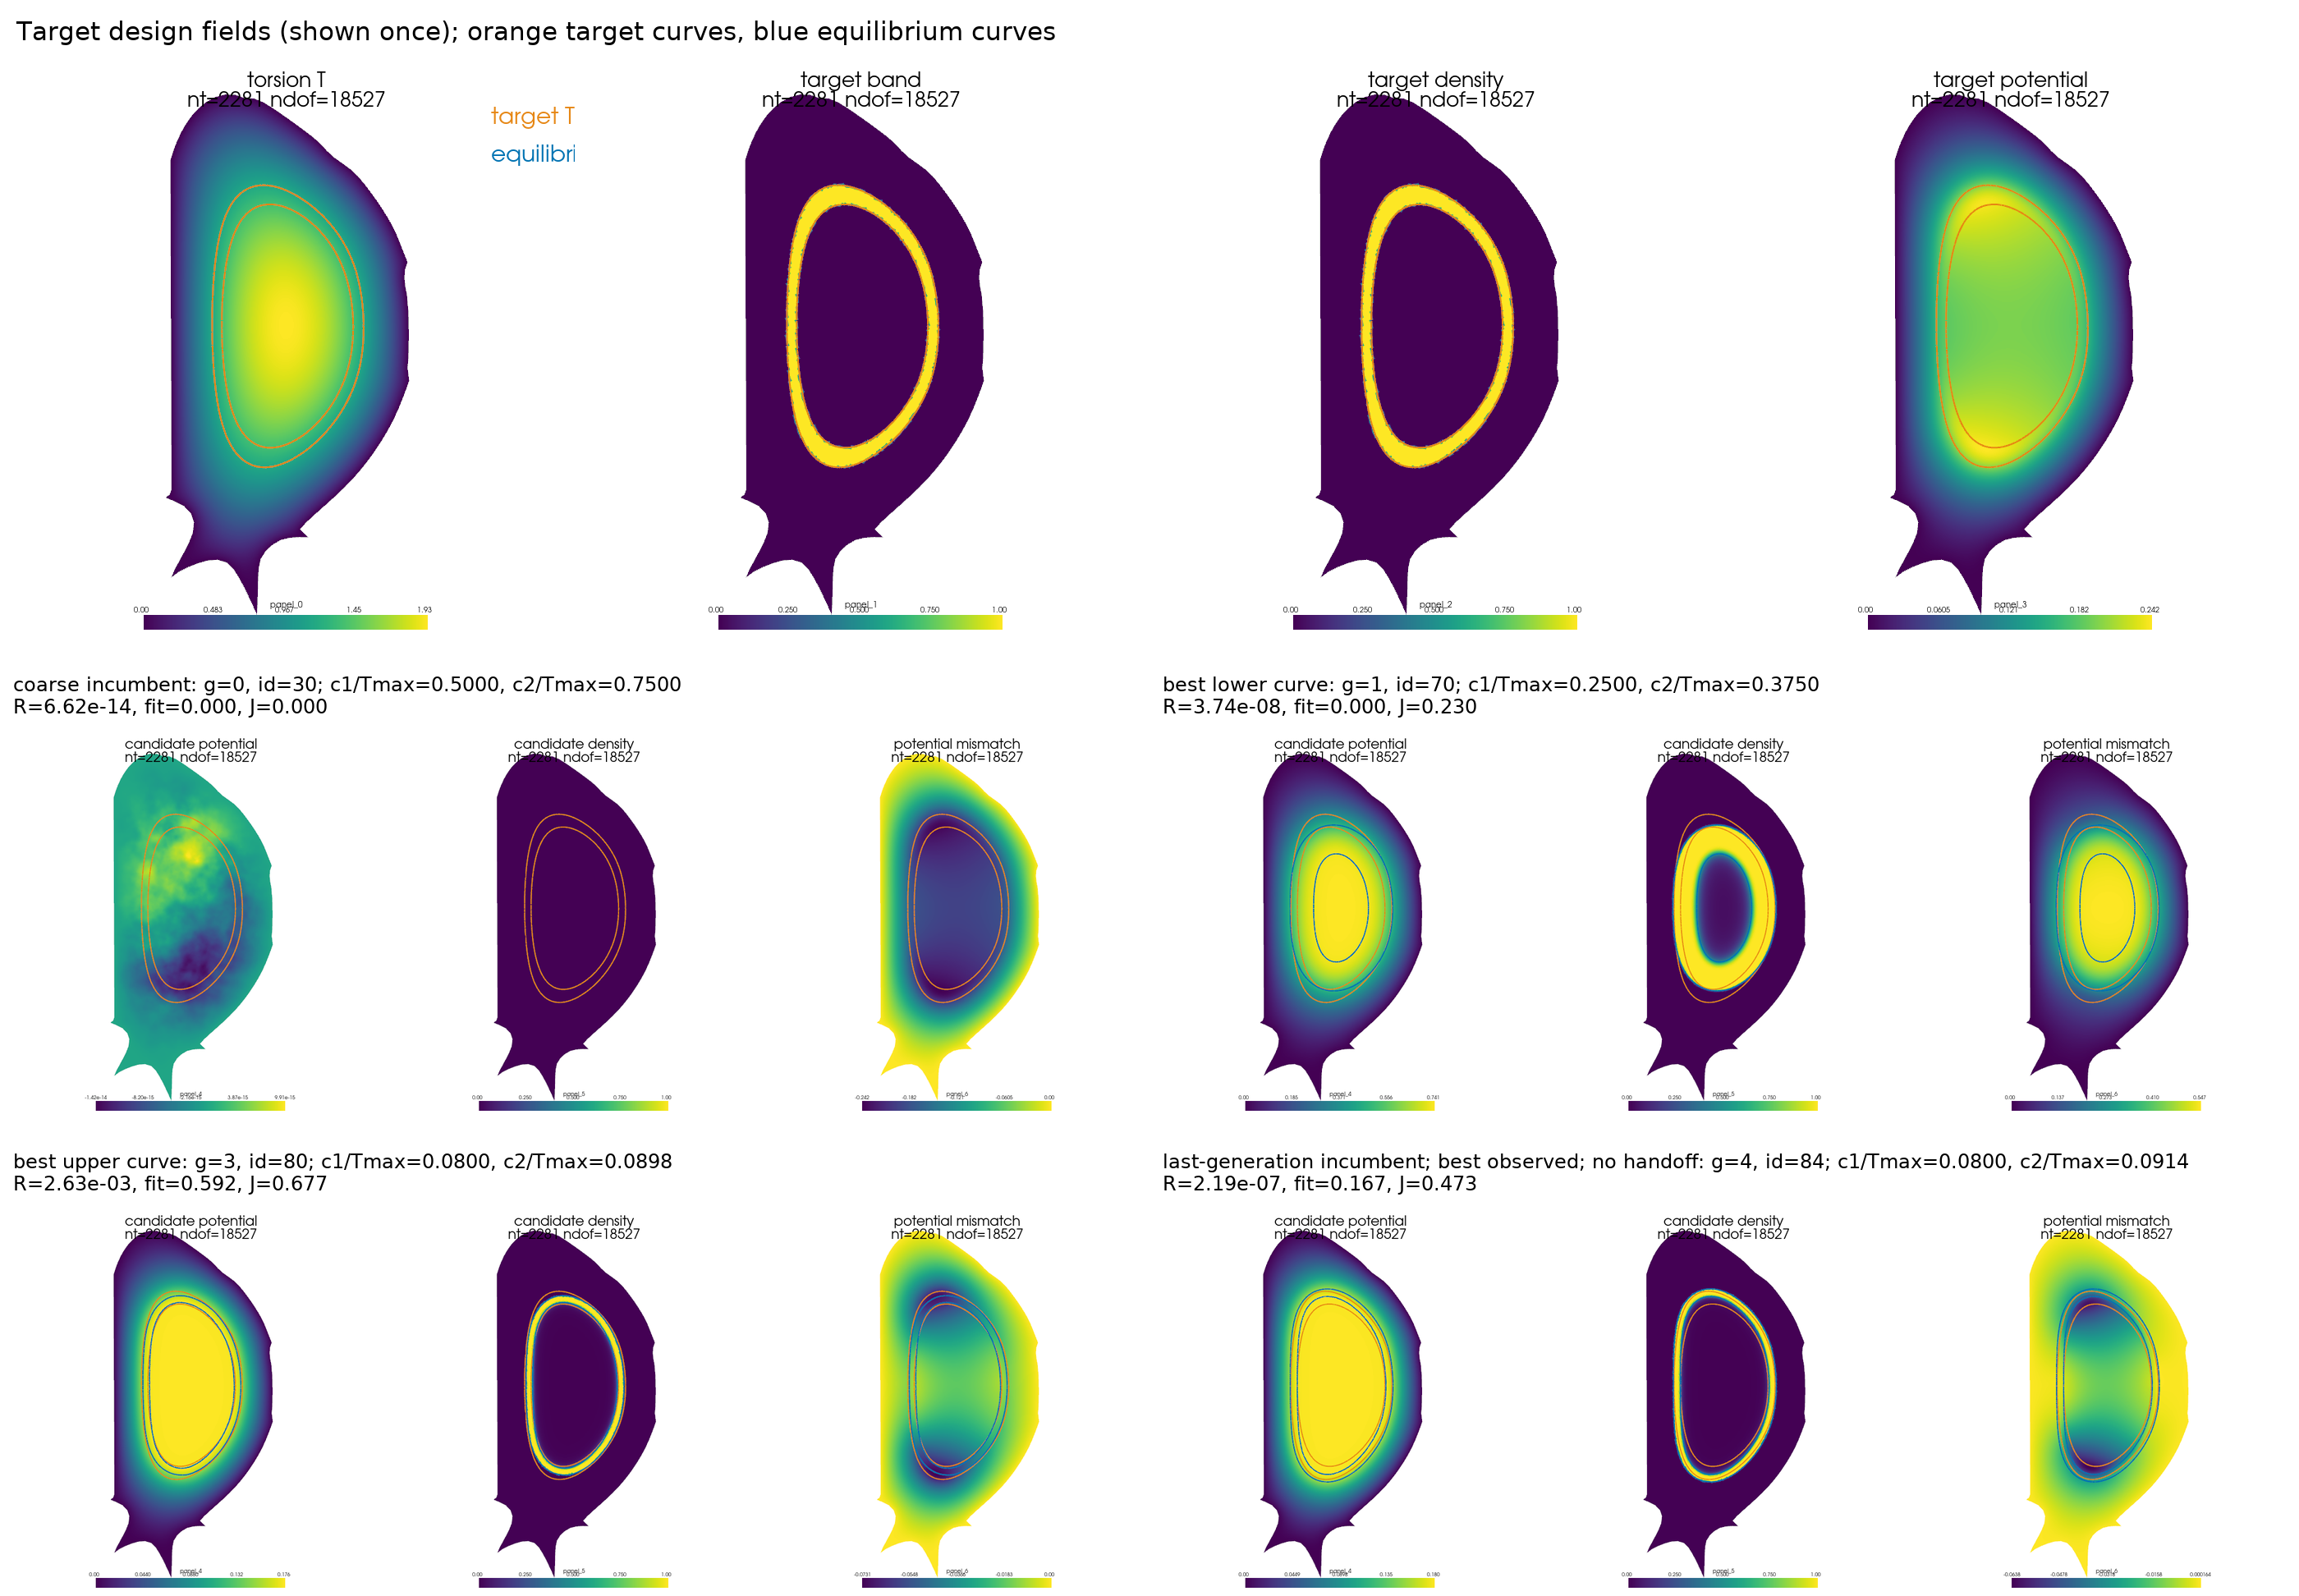
\includegraphics[width=0.96\linewidth,height=0.76\textheight,keepaspectratio]{figures/iter_0p6_0p7_adaptive_continuation_eps002_lowdof_candidate_storyboard.png}
\caption{Design-once v2 candidate storyboard.  The fixed torsion, target band,
target density, and target potential appear only in the upper strip.  The
candidate rows then retain the coarse incumbent, the best individual curve
fits (including candidate 80), and the last-generation/PDE-qualified
diagnostic best candidate 84.  Orange target and blue equilibrium contours
are drawn over complete rank-zero-gathered fields with the mesh hidden.  No
optimizer-final panel is present because there was no handoff.  Data status:
actual.}
\label{fig:iter-adaptive-v2-storyboard}
\end{figure}

\begin{landscape}
\begin{figure}[tbp]
\centering
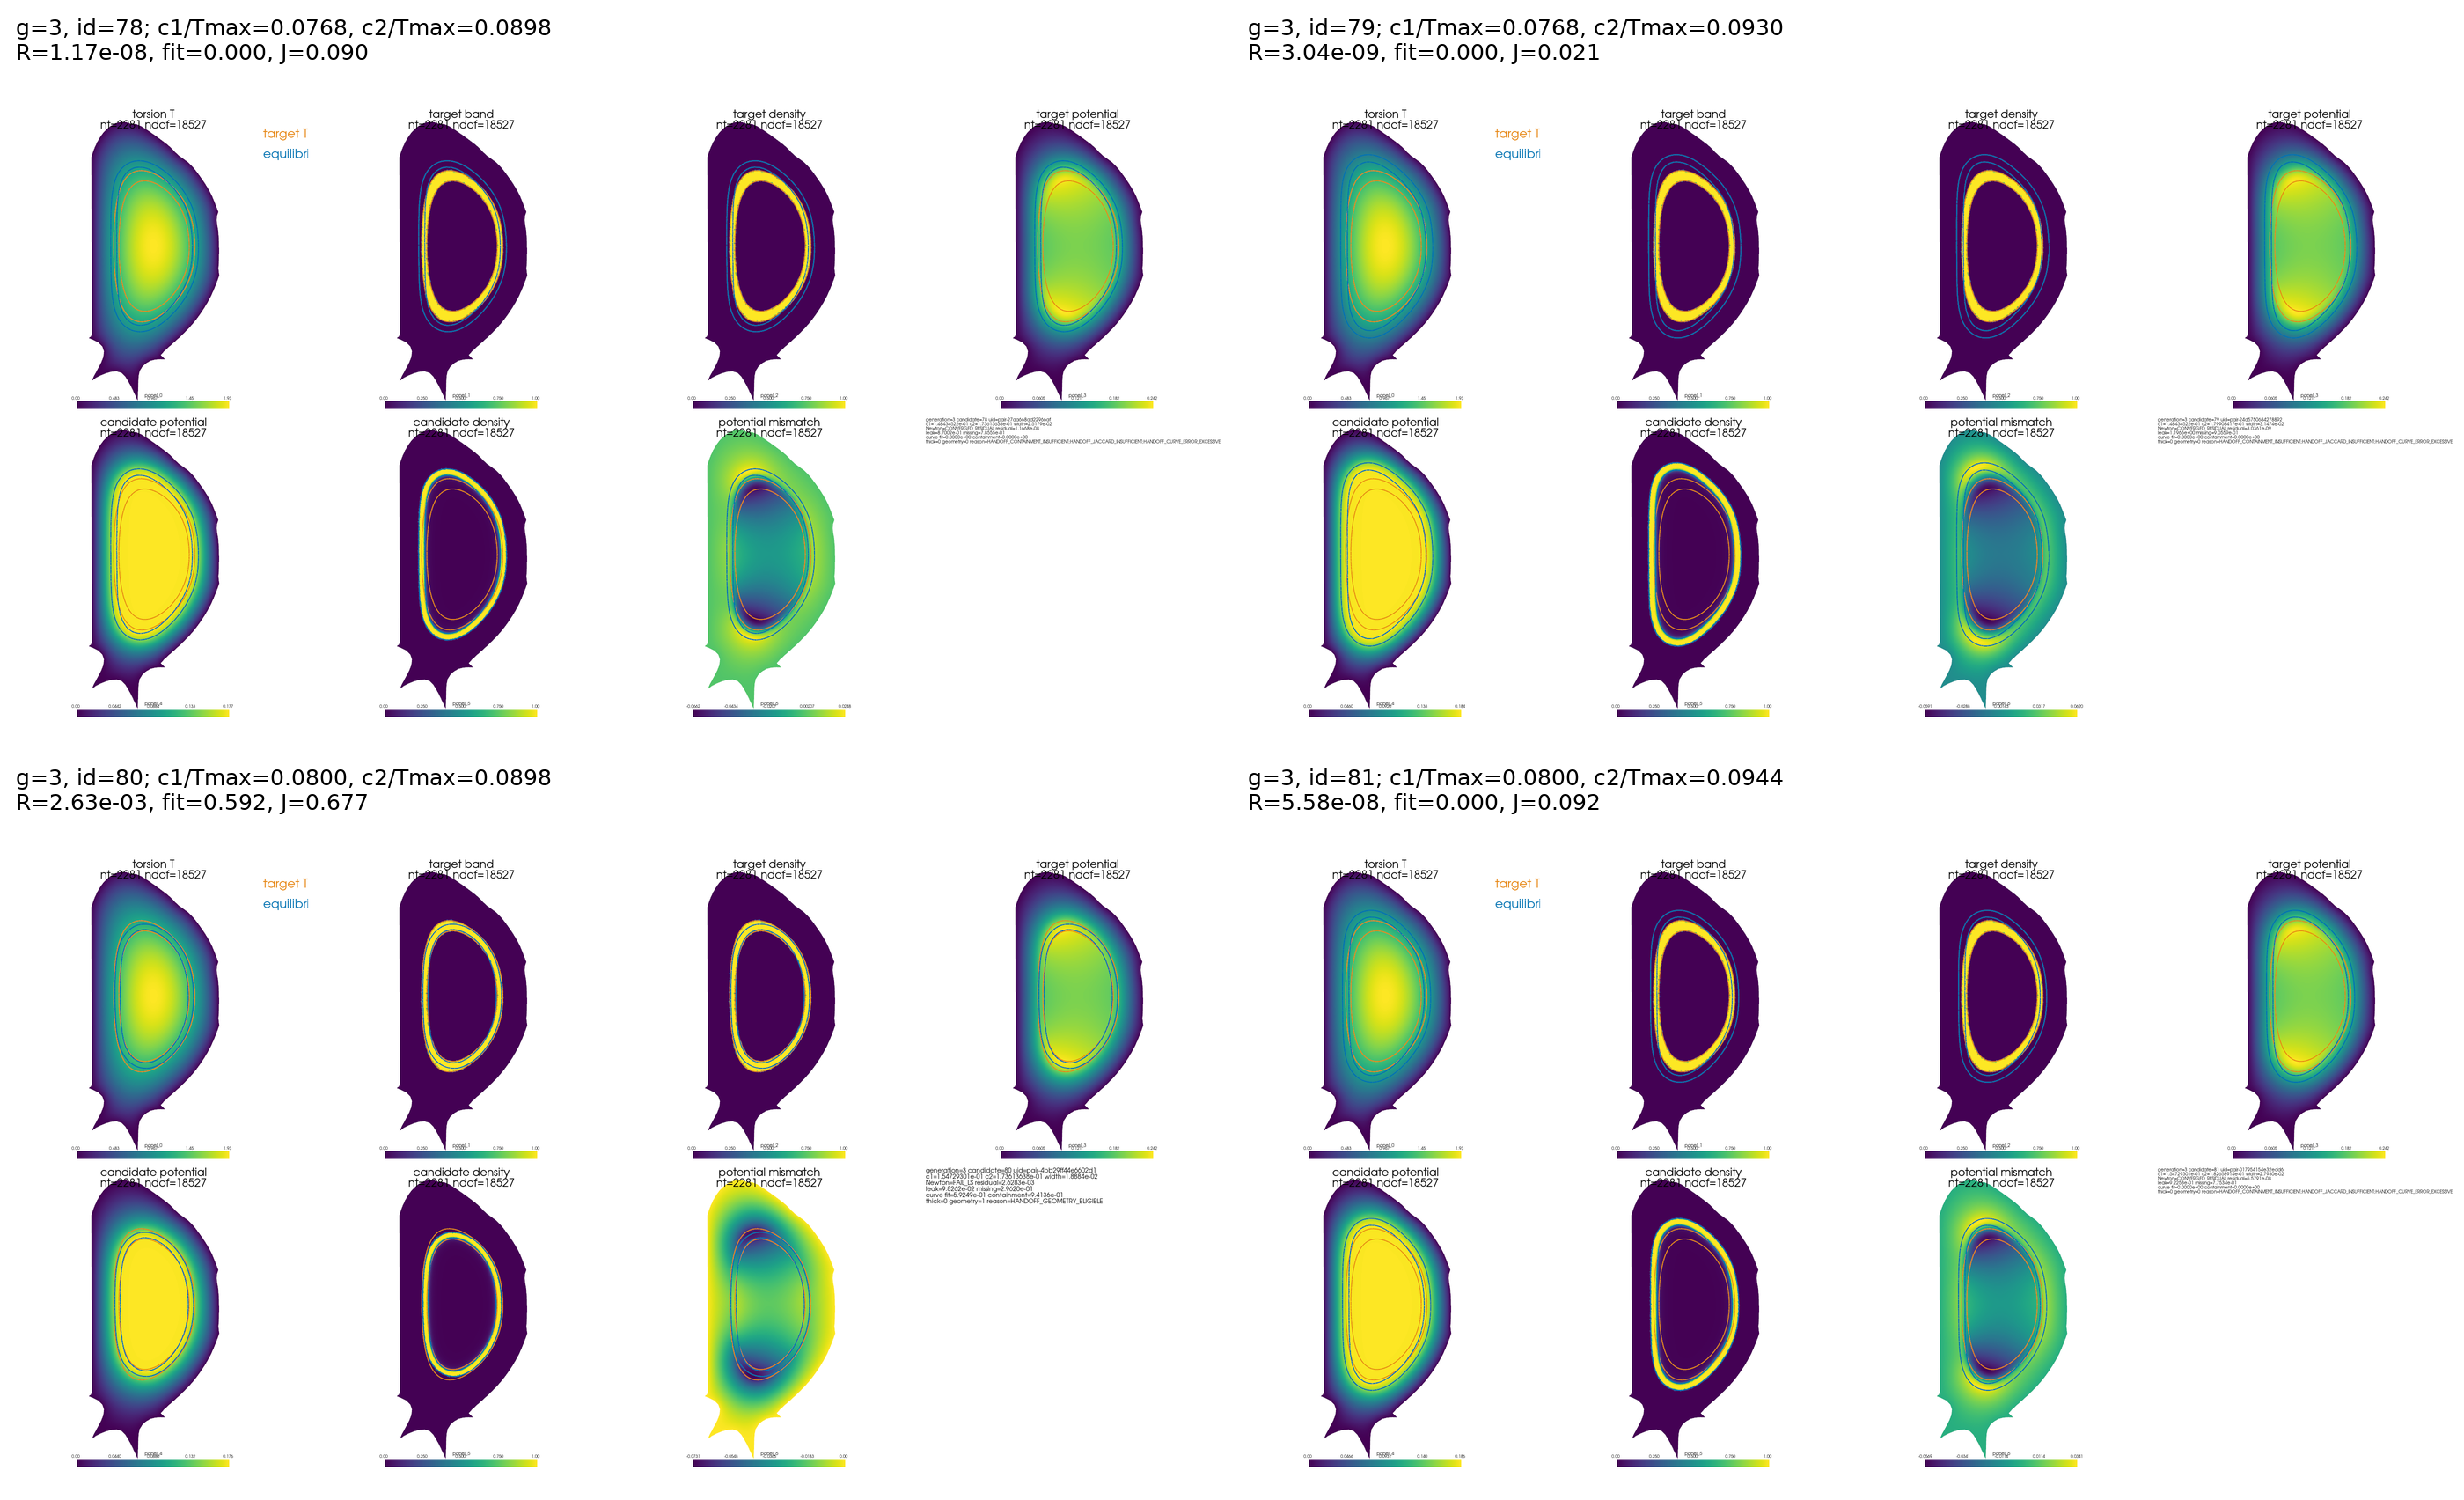
\includegraphics[width=0.49\linewidth]{figures/iter_0p6_0p7_adaptive_continuation_eps002_lowdof_candidate_contact_015.png}
\hfill
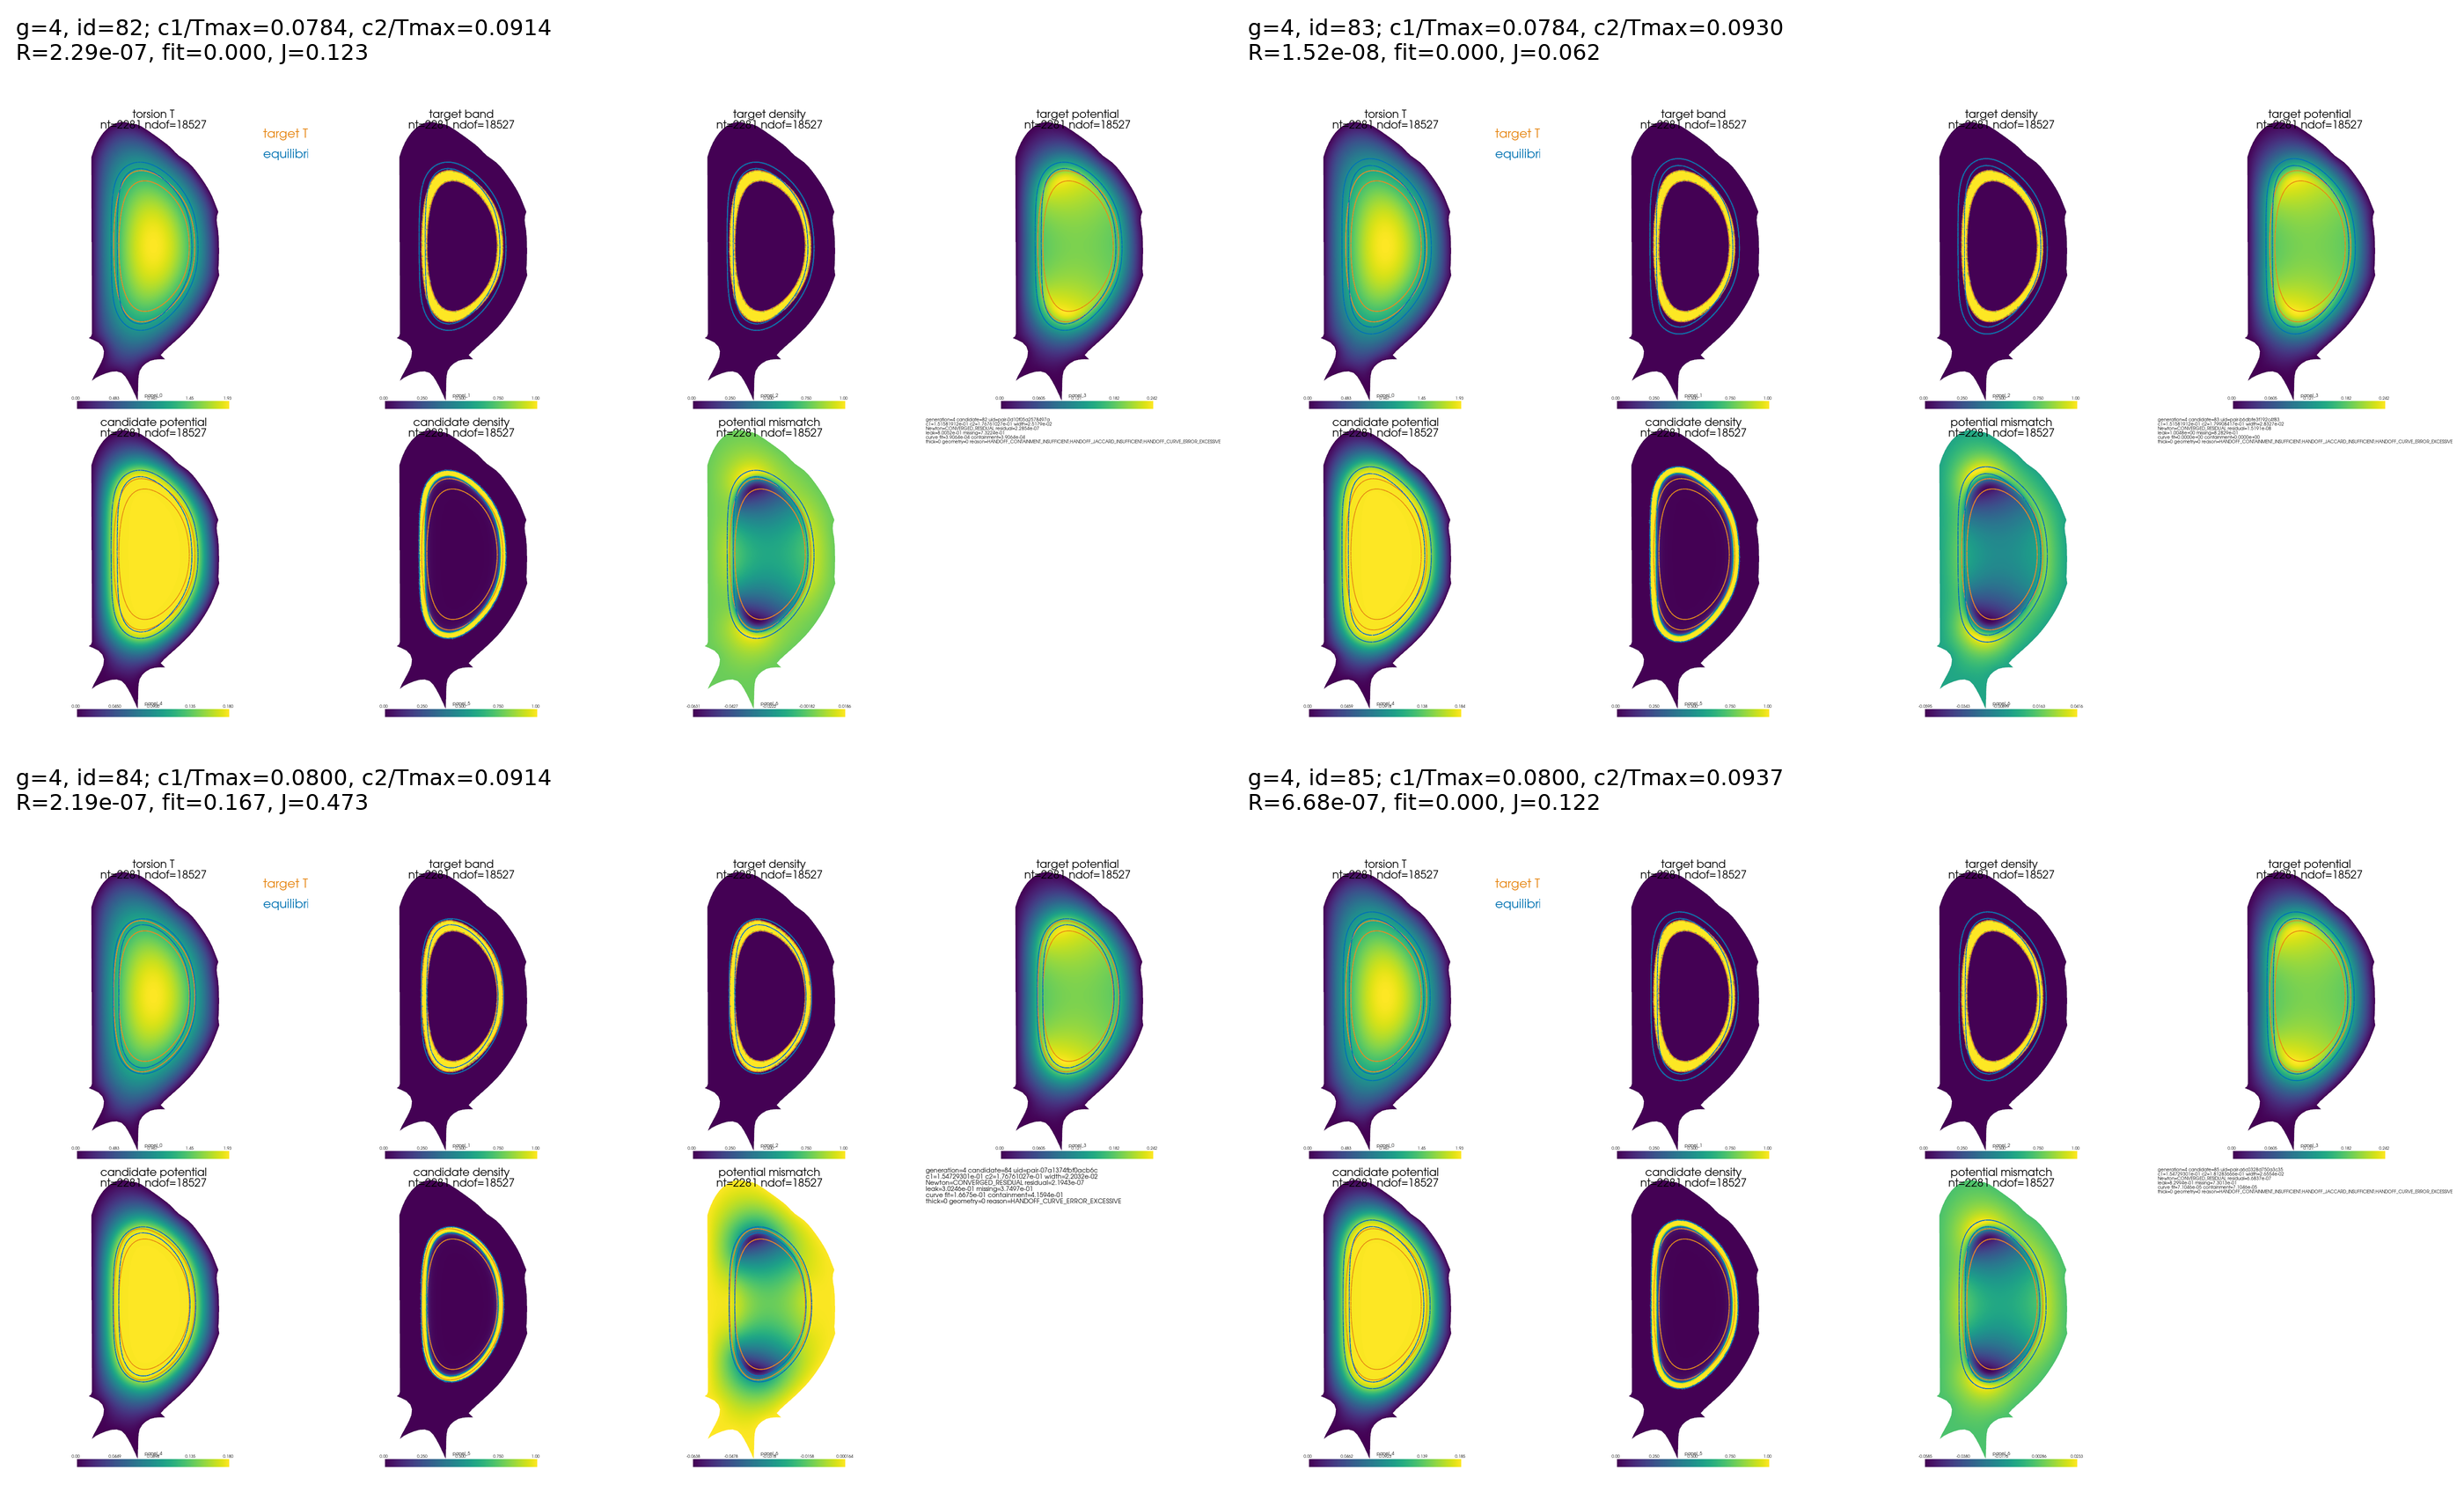
\includegraphics[width=0.49\linewidth]{figures/iter_0p6_0p7_adaptive_continuation_eps002_lowdof_candidate_contact_016.png}
\caption{All 64 v2 solved candidates have a validated individual lossless PNG
and are reproduced in 16 four-candidate contact sheets.  The two late sheets
shown here retain the competing candidates and their neighboring continuation
states.  The left sheet contains
candidates 78--81, with geometry-gate candidate 80 at lower left; the right
contains candidates 82--85, with PDE-qualified diagnostic candidate 84 at
lower left.  Every tile shows all seven gathered fields and both contour
families without mesh edges.  Candidate 80 is rejected by the PDE gate and
candidate 84 by the upper-curve handoff tolerance.  Data status: actual; no
optimizer winner.}
\label{fig:iter-adaptive-v2-contact-late}
\end{figure}
\end{landscape}

\subsection{Adaptive-search handoff on Pacman and horseshoe}
\label{sec:adaptive-pacman-horseshoe}

The continuation-aware two-level-curve search was next applied without any
threshold prior to the Pacman band
$[\alpha_{T1},\alpha_{T2}]=[0.55,0.645]$ and the horseshoe band
$[0.14,0.255]$.  Both tests used sharp torsion indicators, $P_4$ elements on
$h=0.075$ meshes, relative equilibrium smoothing
$\varepsilon_\phi/(c_{2,\phi}-c_{1,\phi})=0.16$, and MUMPS.  The Pacman and
horseshoe systems contained respectively $8{,}933$ and $10{,}069$ global
degrees of freedom.  Candidate work used 20 independent one-rank groups,
while the exact handoff and reduced optimization used four ranks.  Thus the
candidate search exploited the workstation without contaminating one Newton
solve with excessive direct-solver communication.

Table~\ref{tab:adaptive-pacman-horseshoe} reports the search outcome.  A
\emph{loose handoff} means that the $10^{-6}$ candidate residual, physical
bounds, and permissive curve/overlap gate were passed.  The strict gate also
requires the target band and both boundary fits to be resolved at this mesh.
No candidate passed that strict gate on either geometry.  In particular, the
search did find visually plausible and PDE-qualified states, but this is not
equivalent to finding a state stable under an exact Newton correction.

\begin{table}[tbp]
\centering
\caption{Continuation-aware adaptive searches on Pacman and horseshoe.  Every
solved pair, including failures, has an individual rank-zero-gathered PNG.
Data status: actual.}
\label{tab:adaptive-pacman-horseshoe}
\begin{tabular}{lrrrrrrr}
\toprule
Geometry & DOFs & Solved & PDE gate & Loose & Strict & Winner & Residual \\
\midrule
Pacman & 8,933 & 109 & 83 & 38 & 0 & 72 & $4.546\times10^{-8}$ \\
Horseshoe & 10,069 & 54 & 25 & 3 & 0 & 8 & $2.246\times10^{-7}$ \\
\bottomrule
\end{tabular}
\end{table}

Pacman candidate 72 has
$(c_{1,\phi},c_{2,\phi})=(0.00479132,0.00539360)$, hard-band Jaccard index
$0.62716$, paired containment $0.99035$, and search-stage relative leakage
and missing area $(0.23952,0.39560)$.  Tight Newton correction of the same
saved state reduces the residual to $1.801\times10^{-15}$, but changes those
two geometric discrepancies to $(1.11162,0.95309)$.  Horseshoe candidate 8
has $(c_{1,\phi},c_{2,\phi})=(0.000844388,0.00117457)$, Jaccard index
$0.49040$, containment $0.97795$, and search-stage discrepancies
$(0.37817,0.46511)$.  Its exact correction reaches
$5.557\times10^{-15}$, while the discrepancies become
$(0.18766,0.94154)$.  Figure~\ref{fig:adaptive-handoff-inexactness} makes this
loose-to-tight change explicit.  It is direct evidence that an inexact
intermediate Newton state can rank candidate thresholds incorrectly: before
using its Newton matrix for sensitivities, the corrected branch must be
re-certified geometrically, not only by residual.

\begin{landscape}
\begin{figure}[tbp]
\centering
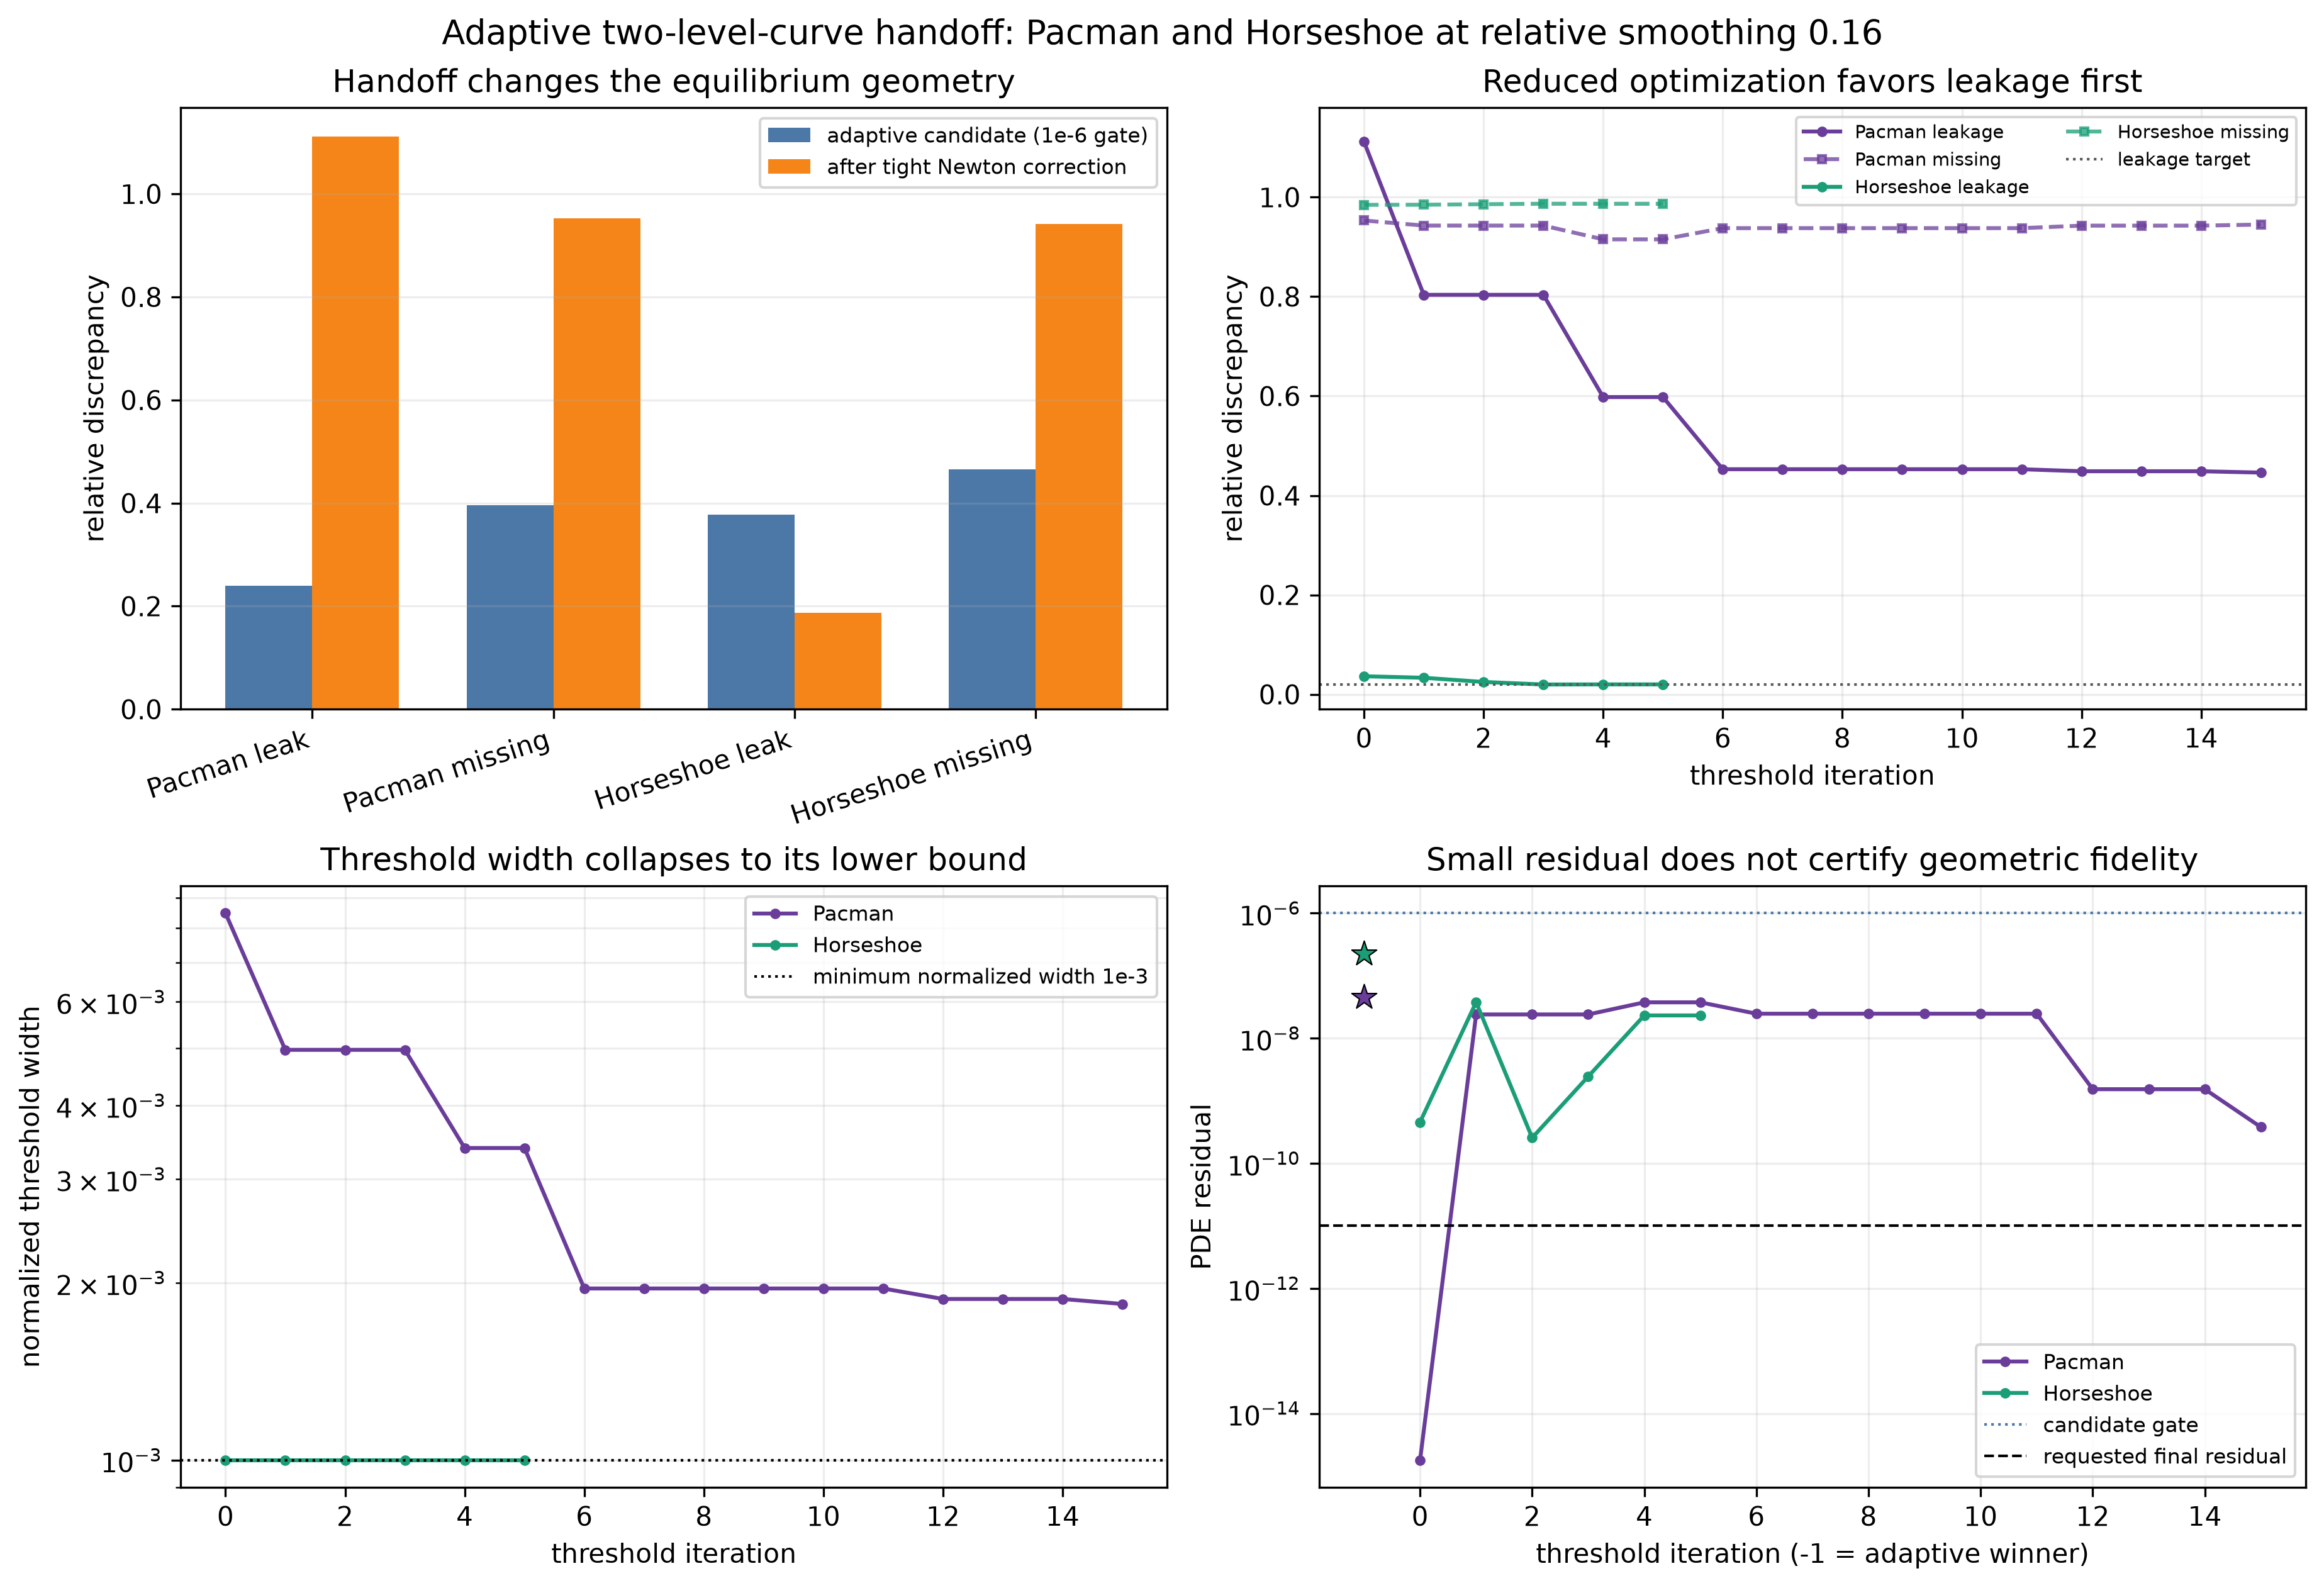
\includegraphics[width=0.94\linewidth,height=0.72\textheight,keepaspectratio]{figures/pacman_horseshoe_adaptive_handoff_inexactness_epsratio0160.png}
\caption{Measured loose-search and tightly corrected handoff behavior.  The
upper-left panel shows that overlap and containment at the candidate tolerance
do not certify the exact branch; the remaining panels show discrepancy,
threshold-width, and nonlinear-residual histories.  Pacman is explicitly a
partial run stopped after iteration 15 at the user's request.  Horseshoe
terminates through a step-too-small condition.  Data status: actual.}
\label{fig:adaptive-handoff-inexactness}
\end{figure}
\end{landscape}

The subsequent threshold iterates expose a second failure mode.  The Pacman
run was stopped after iteration 15, after five accepted steps, and is therefore
reported only as partial: its last state has residual
$3.798\times10^{-10}$, relative leakage $0.44603$, relative missing area
$0.94491$, and active-set Jaccard index $0.10402$.  On horseshoe, five
accepted steps drive the width to the imposed minimum
$6.132\times10^{-5}$ before a \texttt{STEP\_TOO\_SMALL} termination.  The
final projection reaches residual $4.996\times10^{-12}$---adequate for the
general $10^{-11}$ residual requirement, though not the requested
$10^{-12}$ projection tolerance---but relative leakage, missing area, and
Jaccard index are $0.01998$, $0.98673$, and $0.05165$.  It is consequently a
PDE-resolved geometric failure, not a convergence success.  The alternating
leakage-first rule can collapse the threshold width before recovering missing
area; a coupled filter or merit function with exact-branch recertification is
needed before this initialization can be promoted to a robust fallback.

\begin{landscape}
\begin{figure}[tbp]
\centering
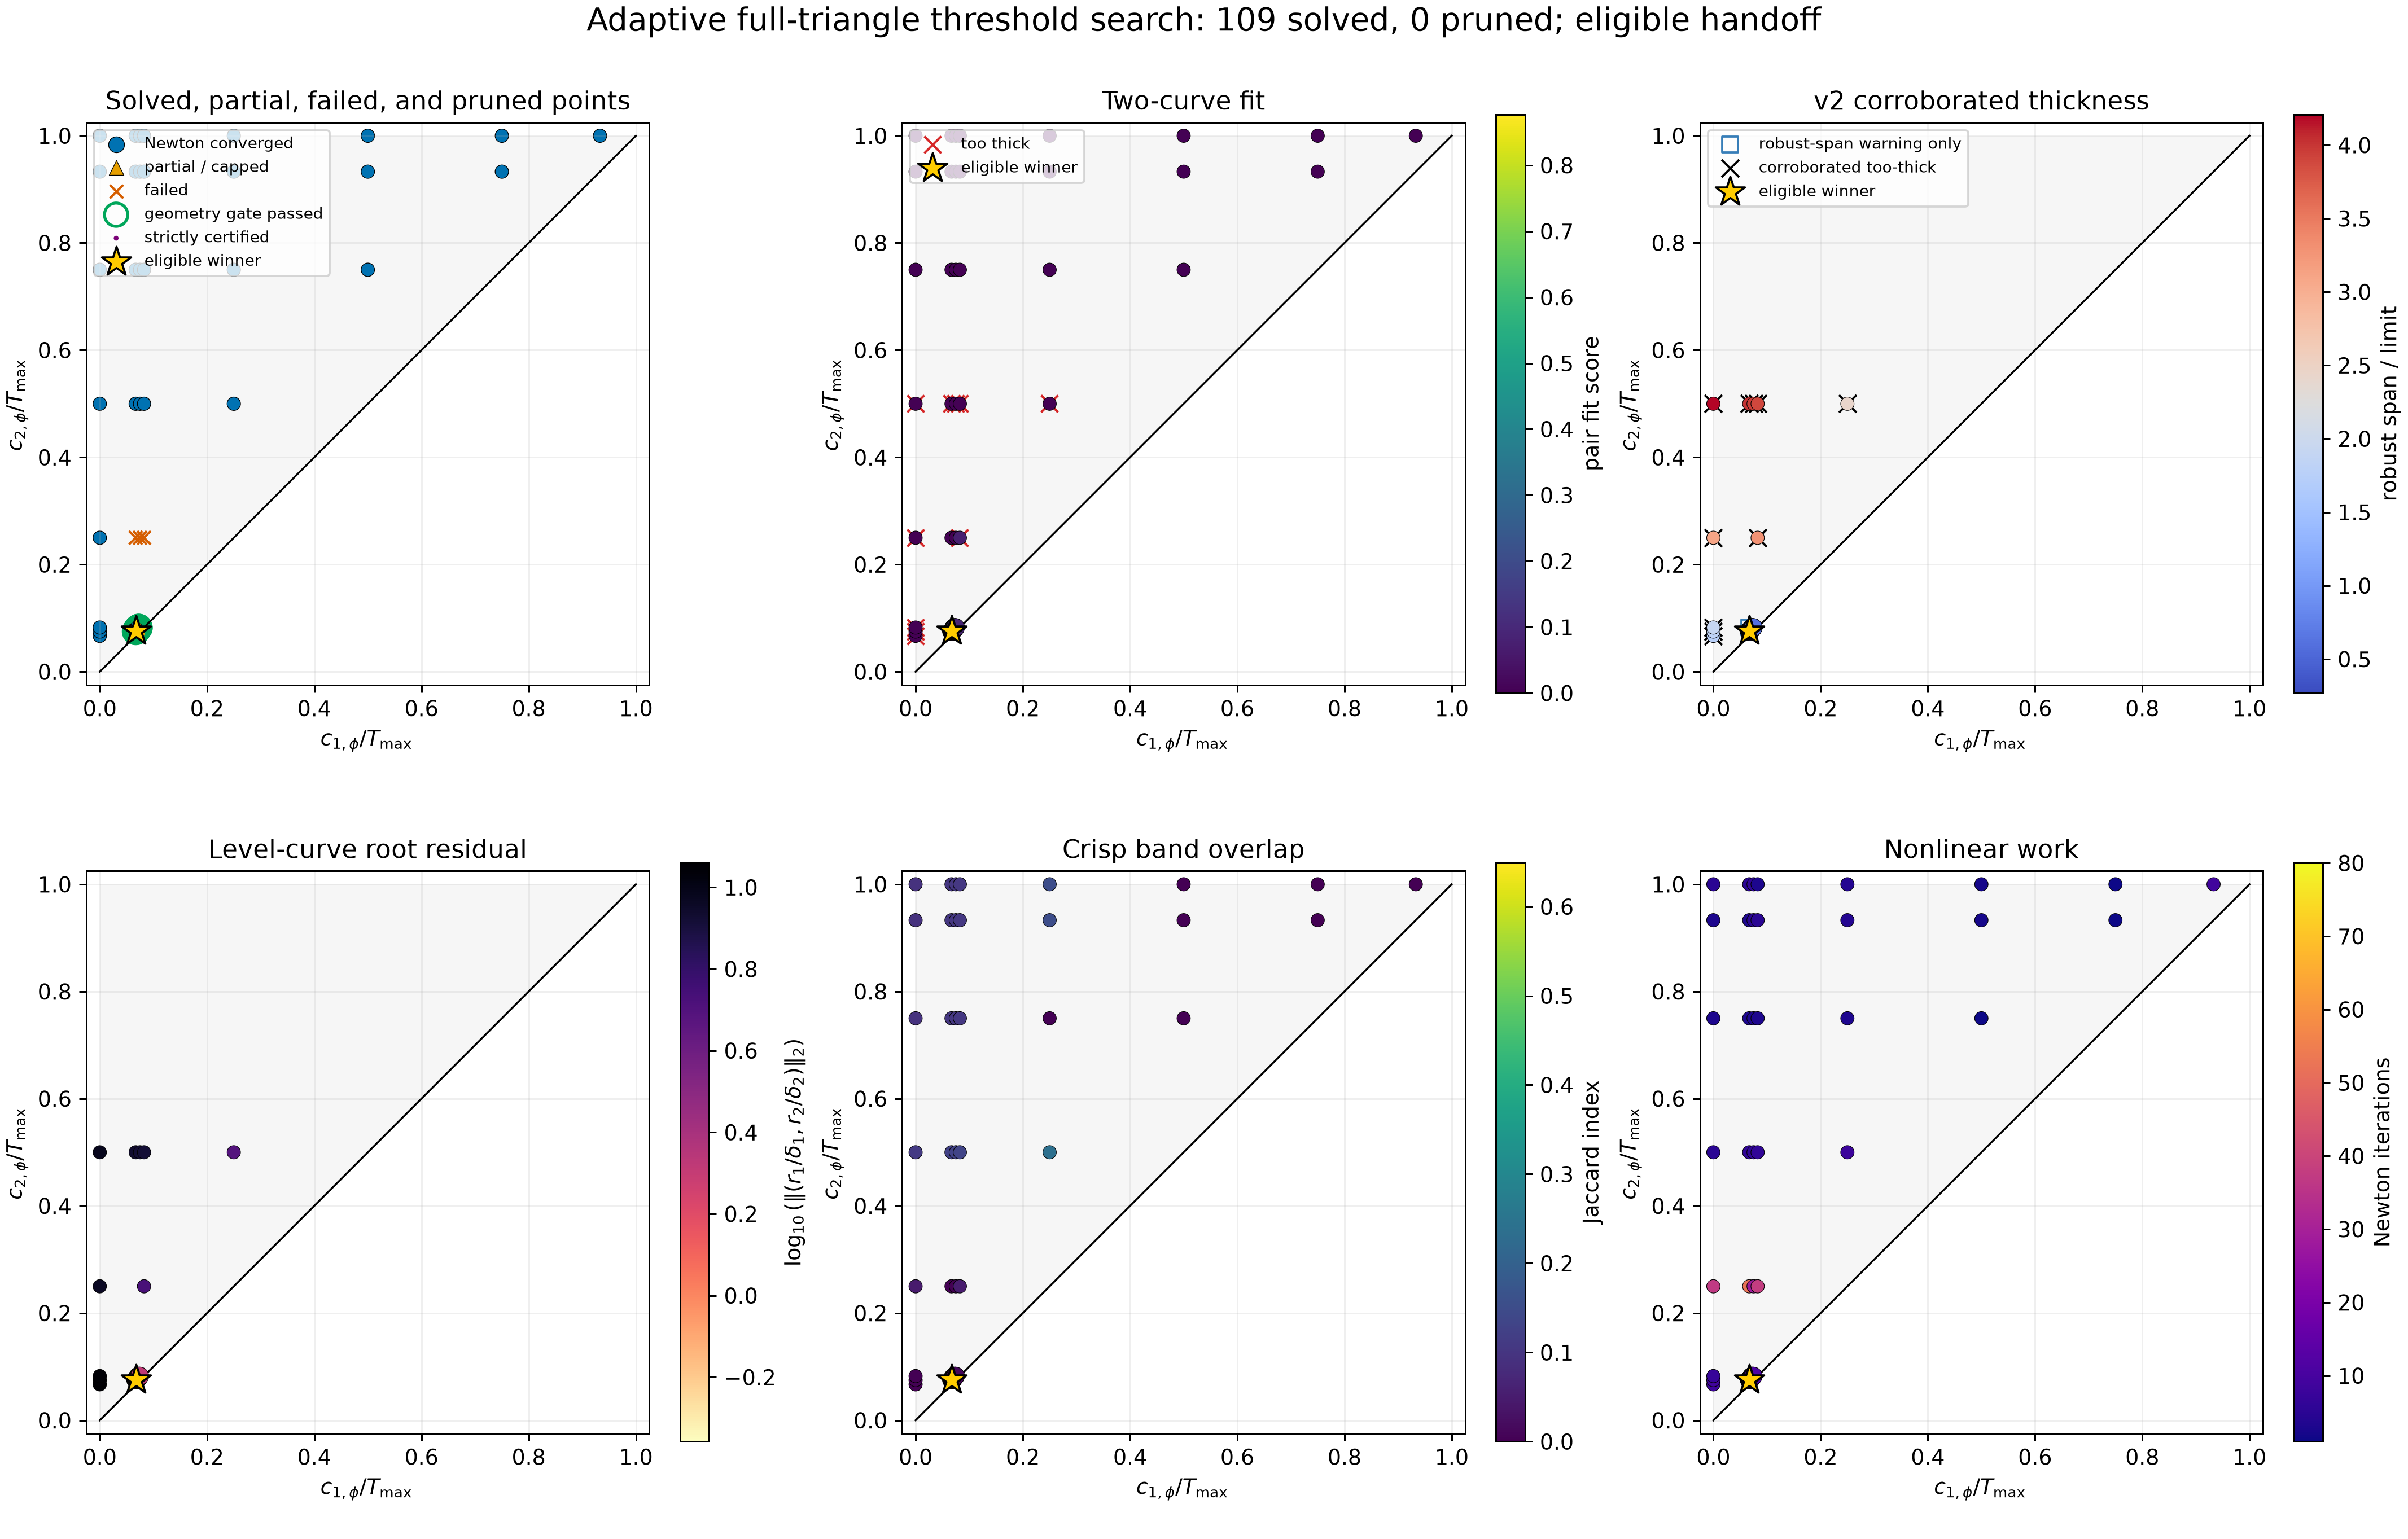
\includegraphics[width=0.49\linewidth]{figures/pacman_0p55_0p645_adaptive_continuation_epsratio0160_search_summary.png}
\hfill
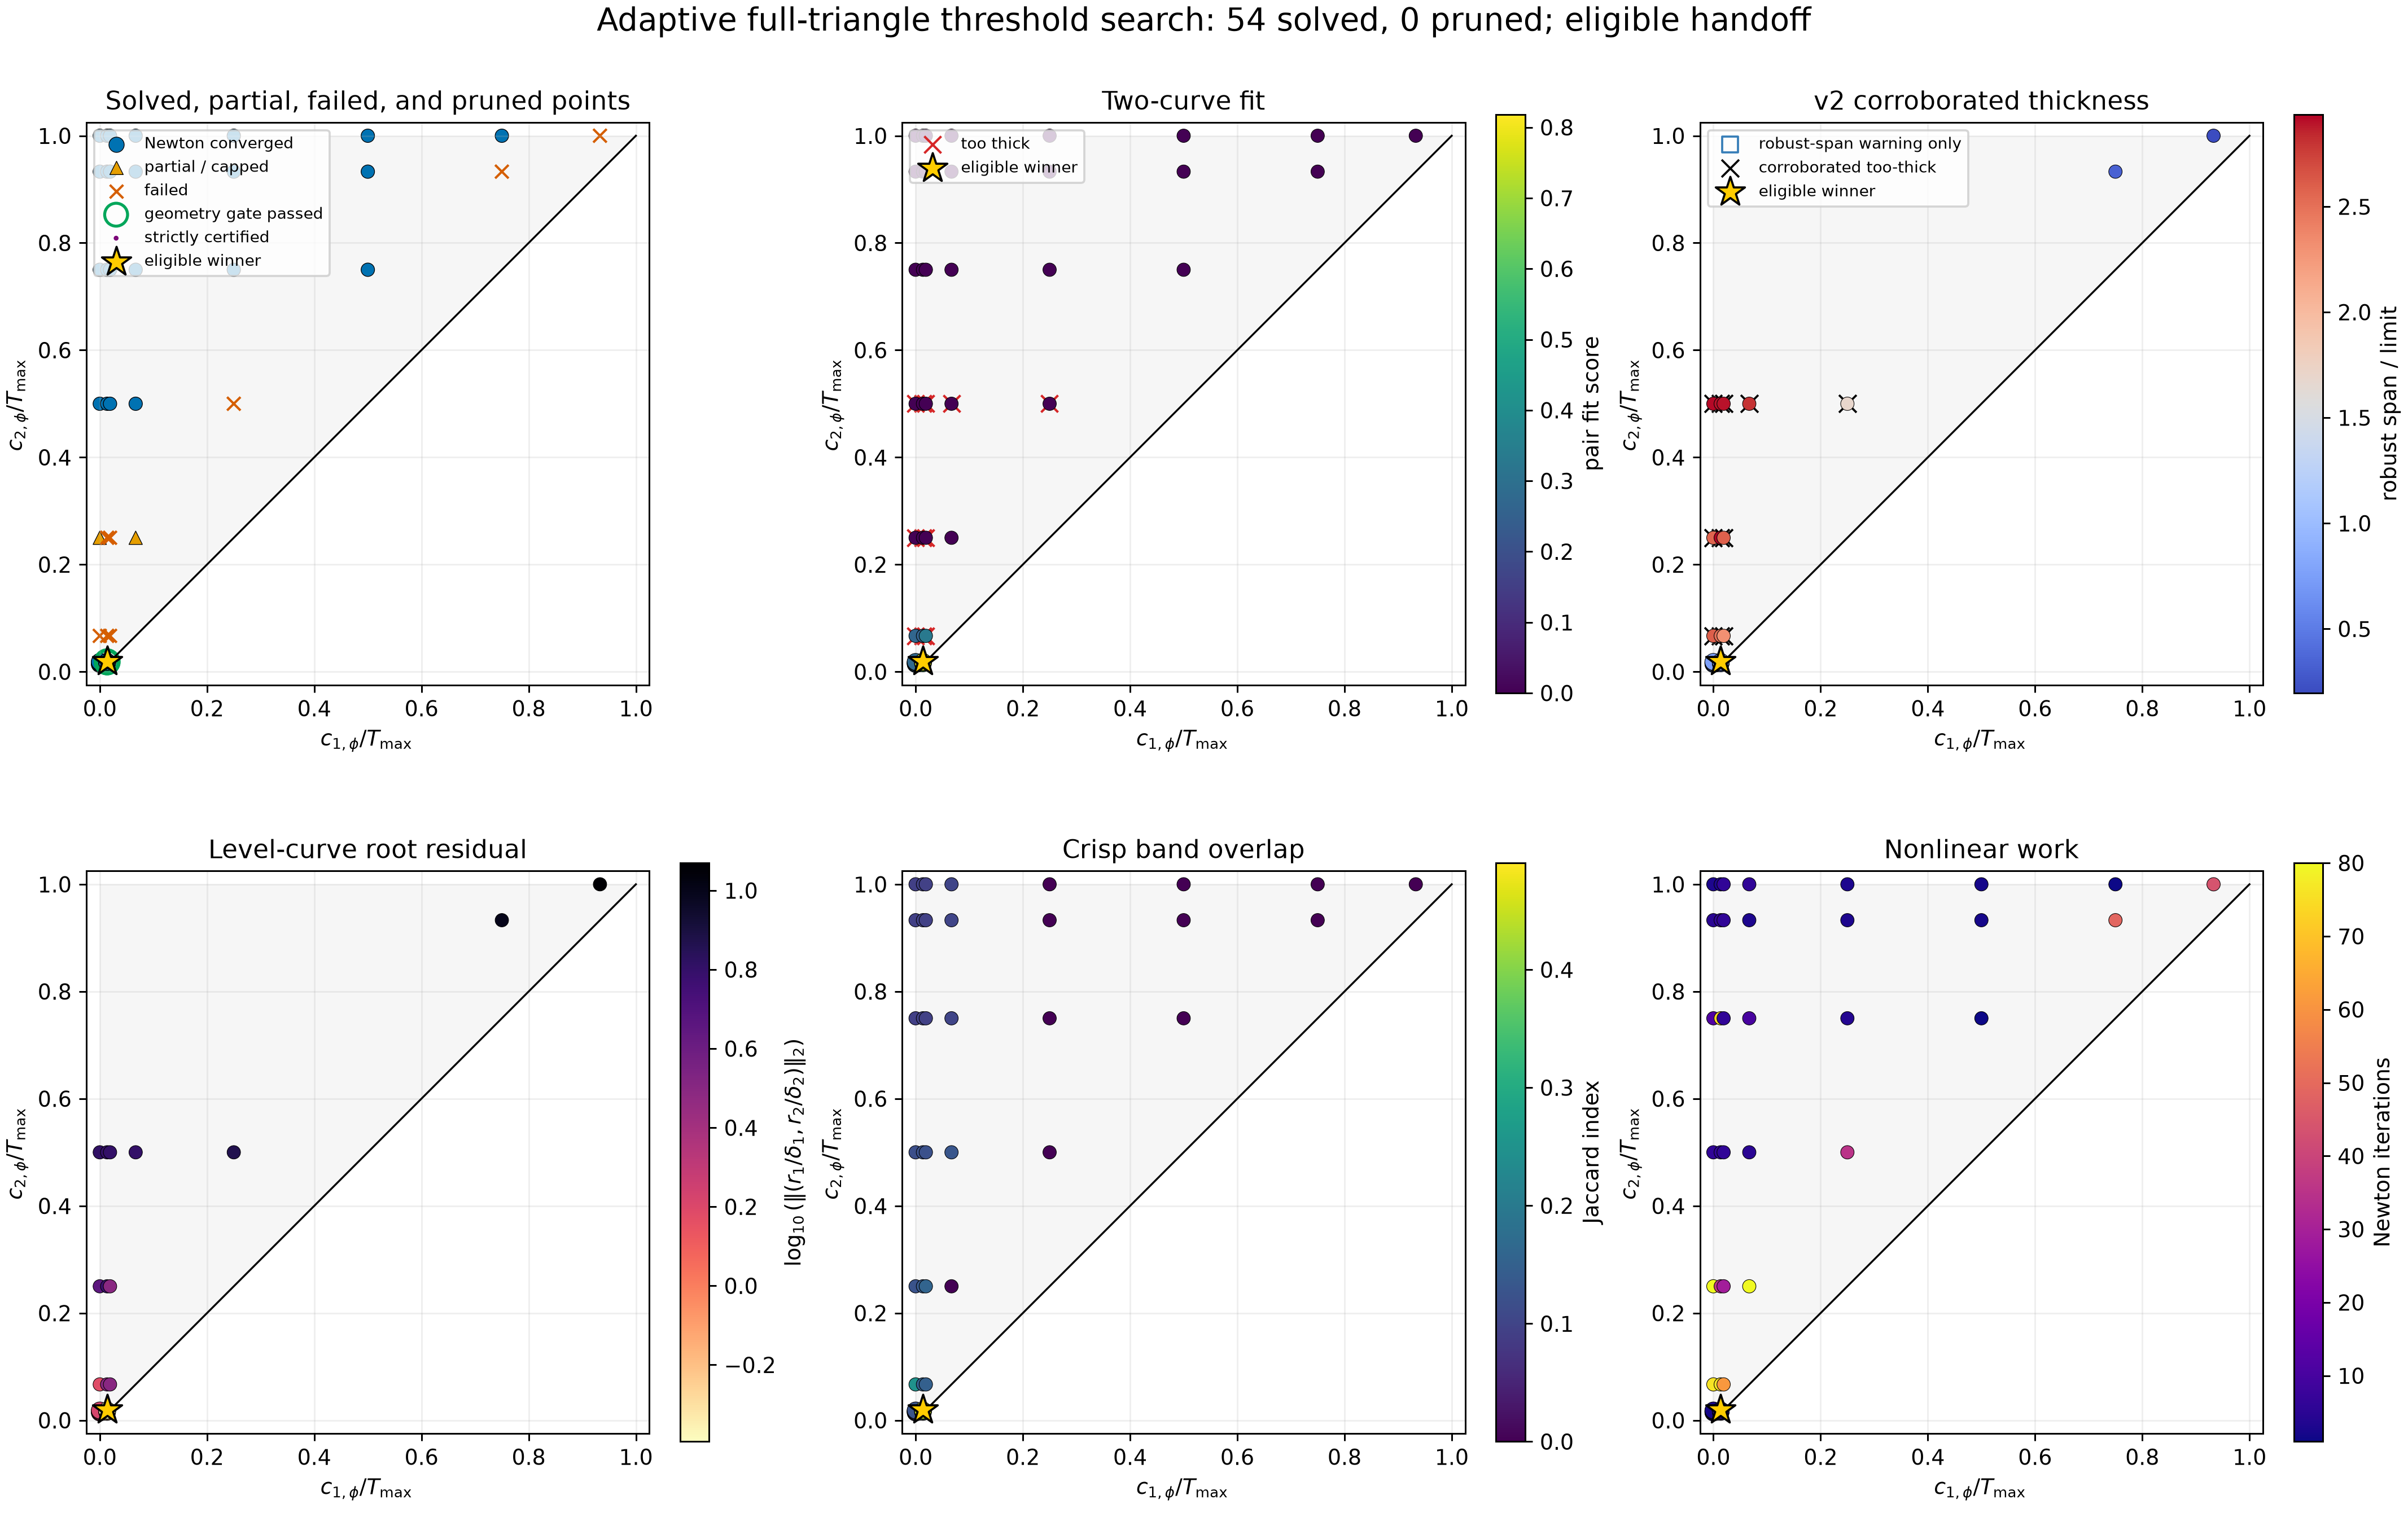
\includegraphics[width=0.49\linewidth]{figures/horseshoe_0p14_0p255_adaptive_continuation_epsratio0160_search_summary.png}
\caption{Full-triangle adaptive-search diagnostics for Pacman (left) and
horseshoe (right).  All unsuccessful, inactive, and PDE-failed candidates are
retained.  The searches solve 109 and 54 candidate pairs respectively, with
no manually supplied threshold location.  Data status: actual.}
\label{fig:adaptive-pacman-horseshoe-search}
\end{figure}
\end{landscape}

\begin{landscape}
\begin{figure}[tbp]
\centering
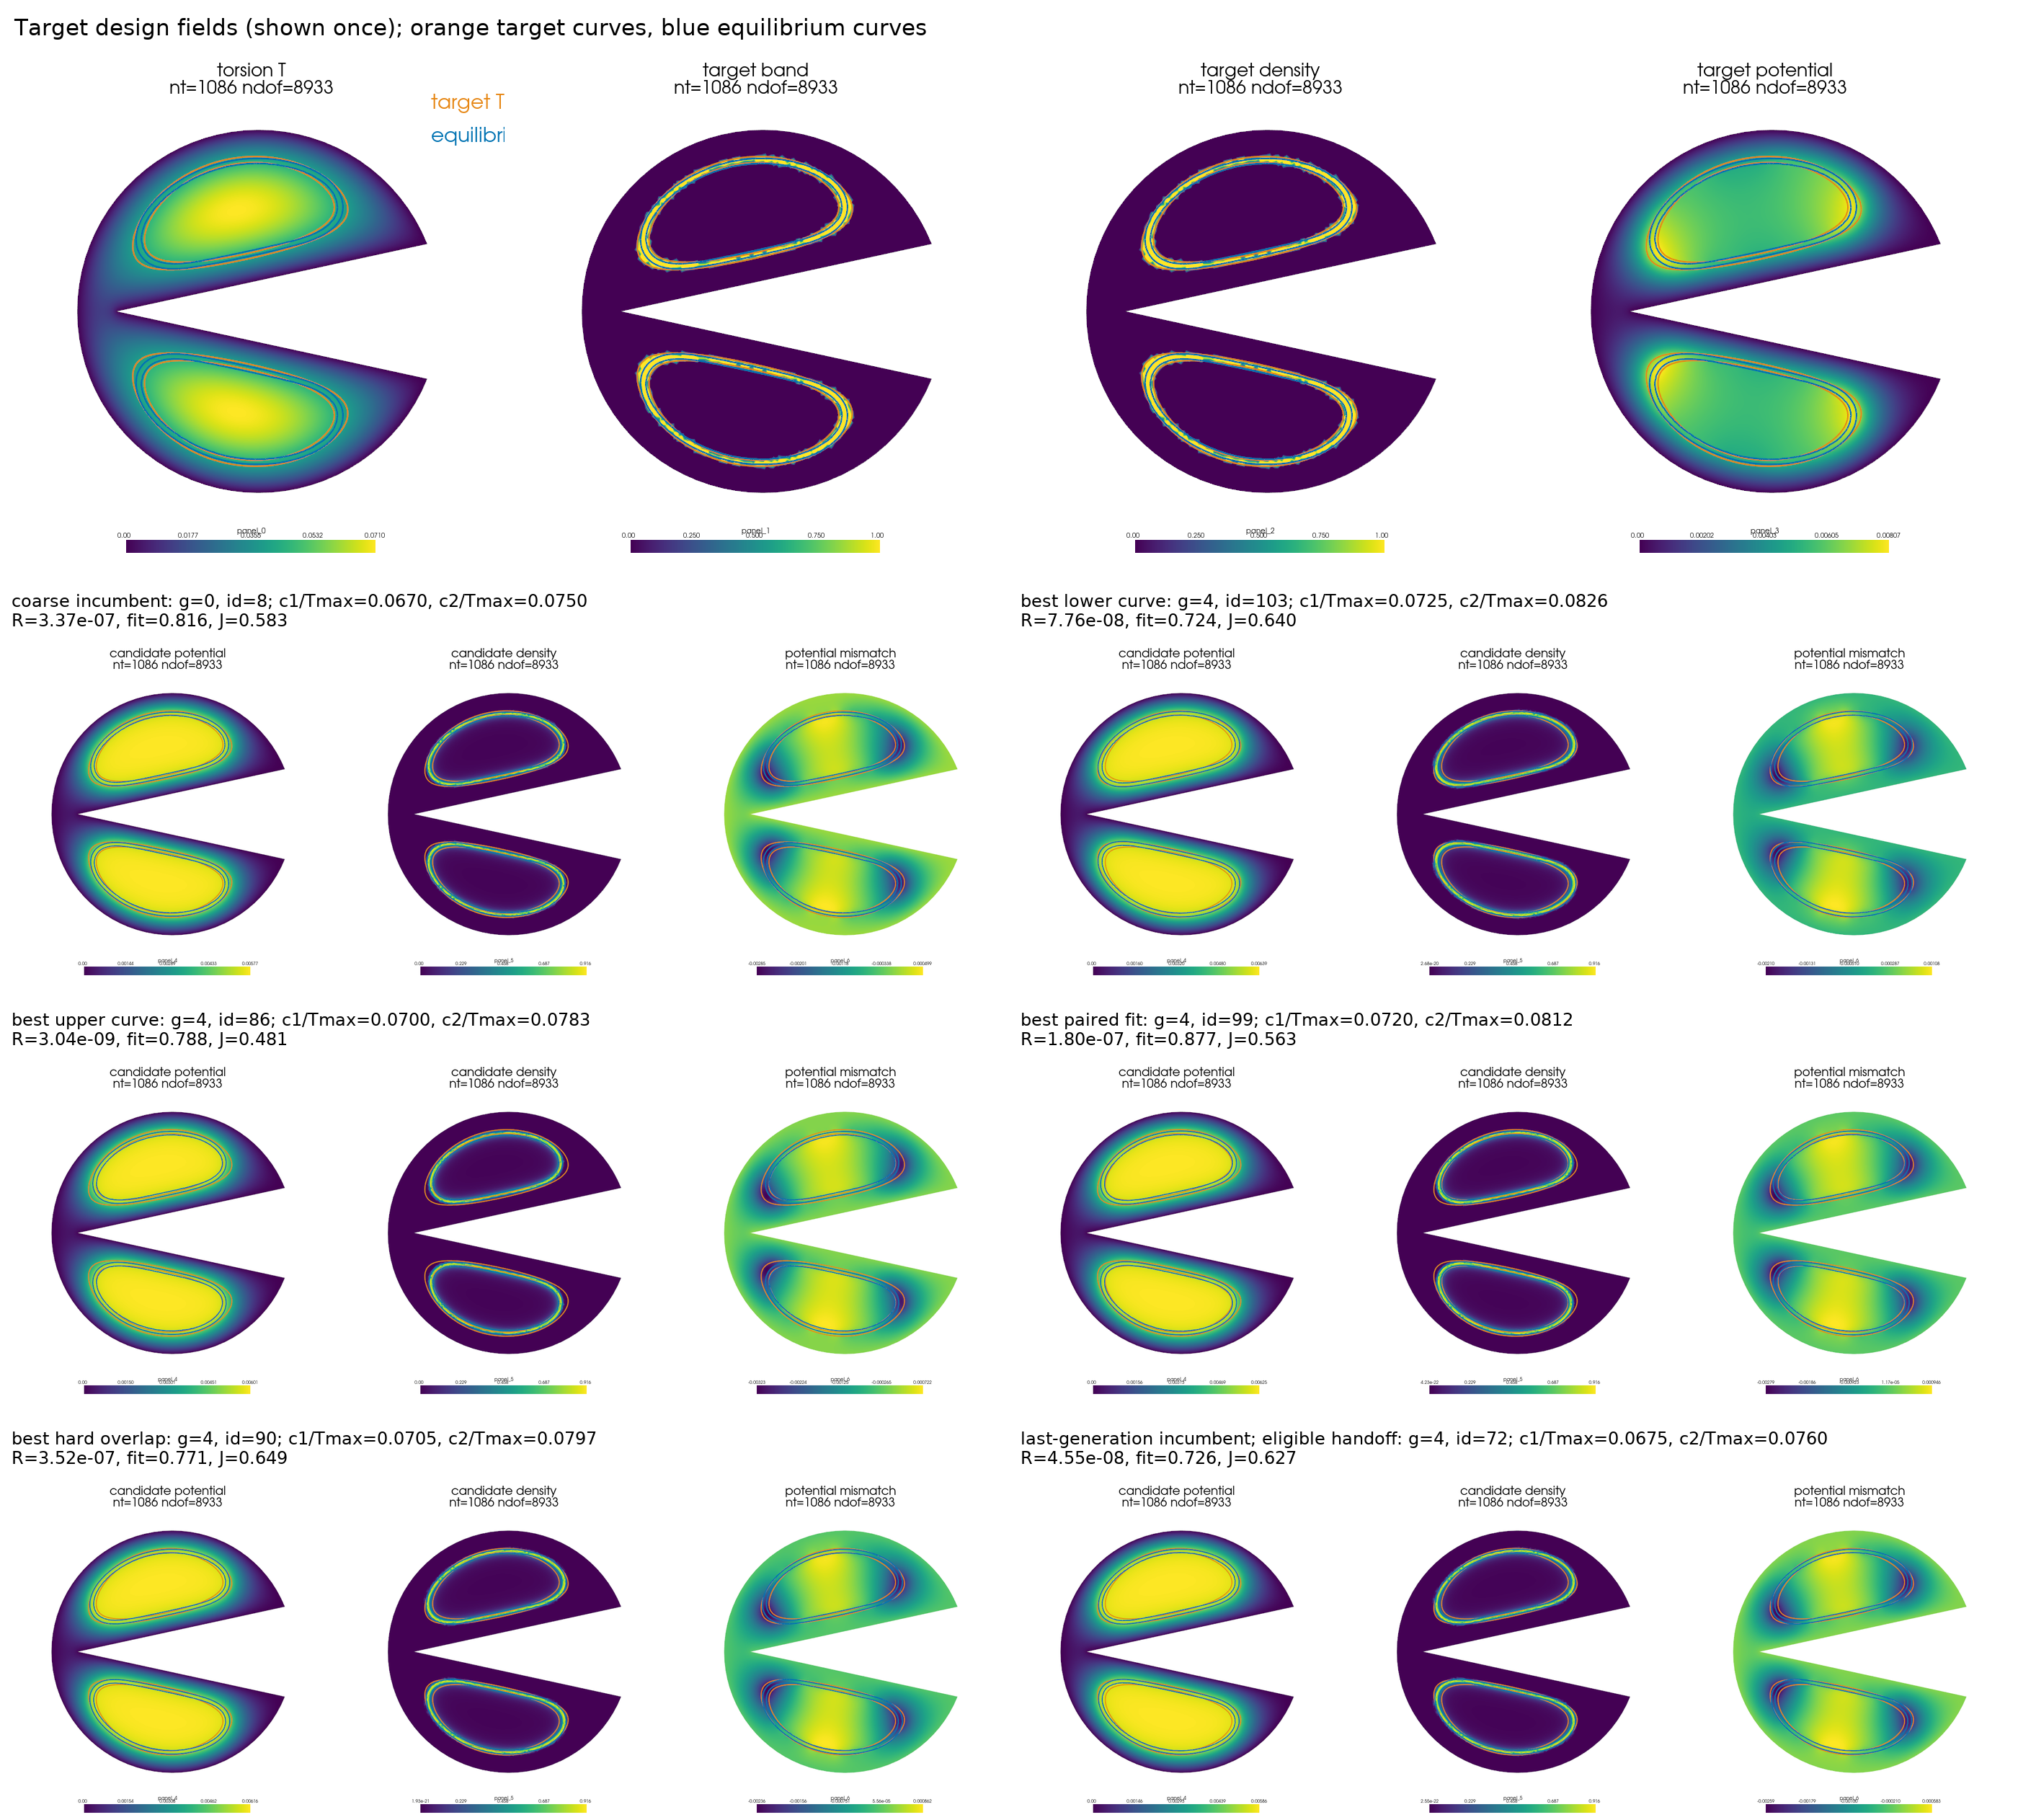
\includegraphics[width=0.49\linewidth]{figures/pacman_0p55_0p645_adaptive_continuation_epsratio0160_candidate_storyboard.png}
\hfill
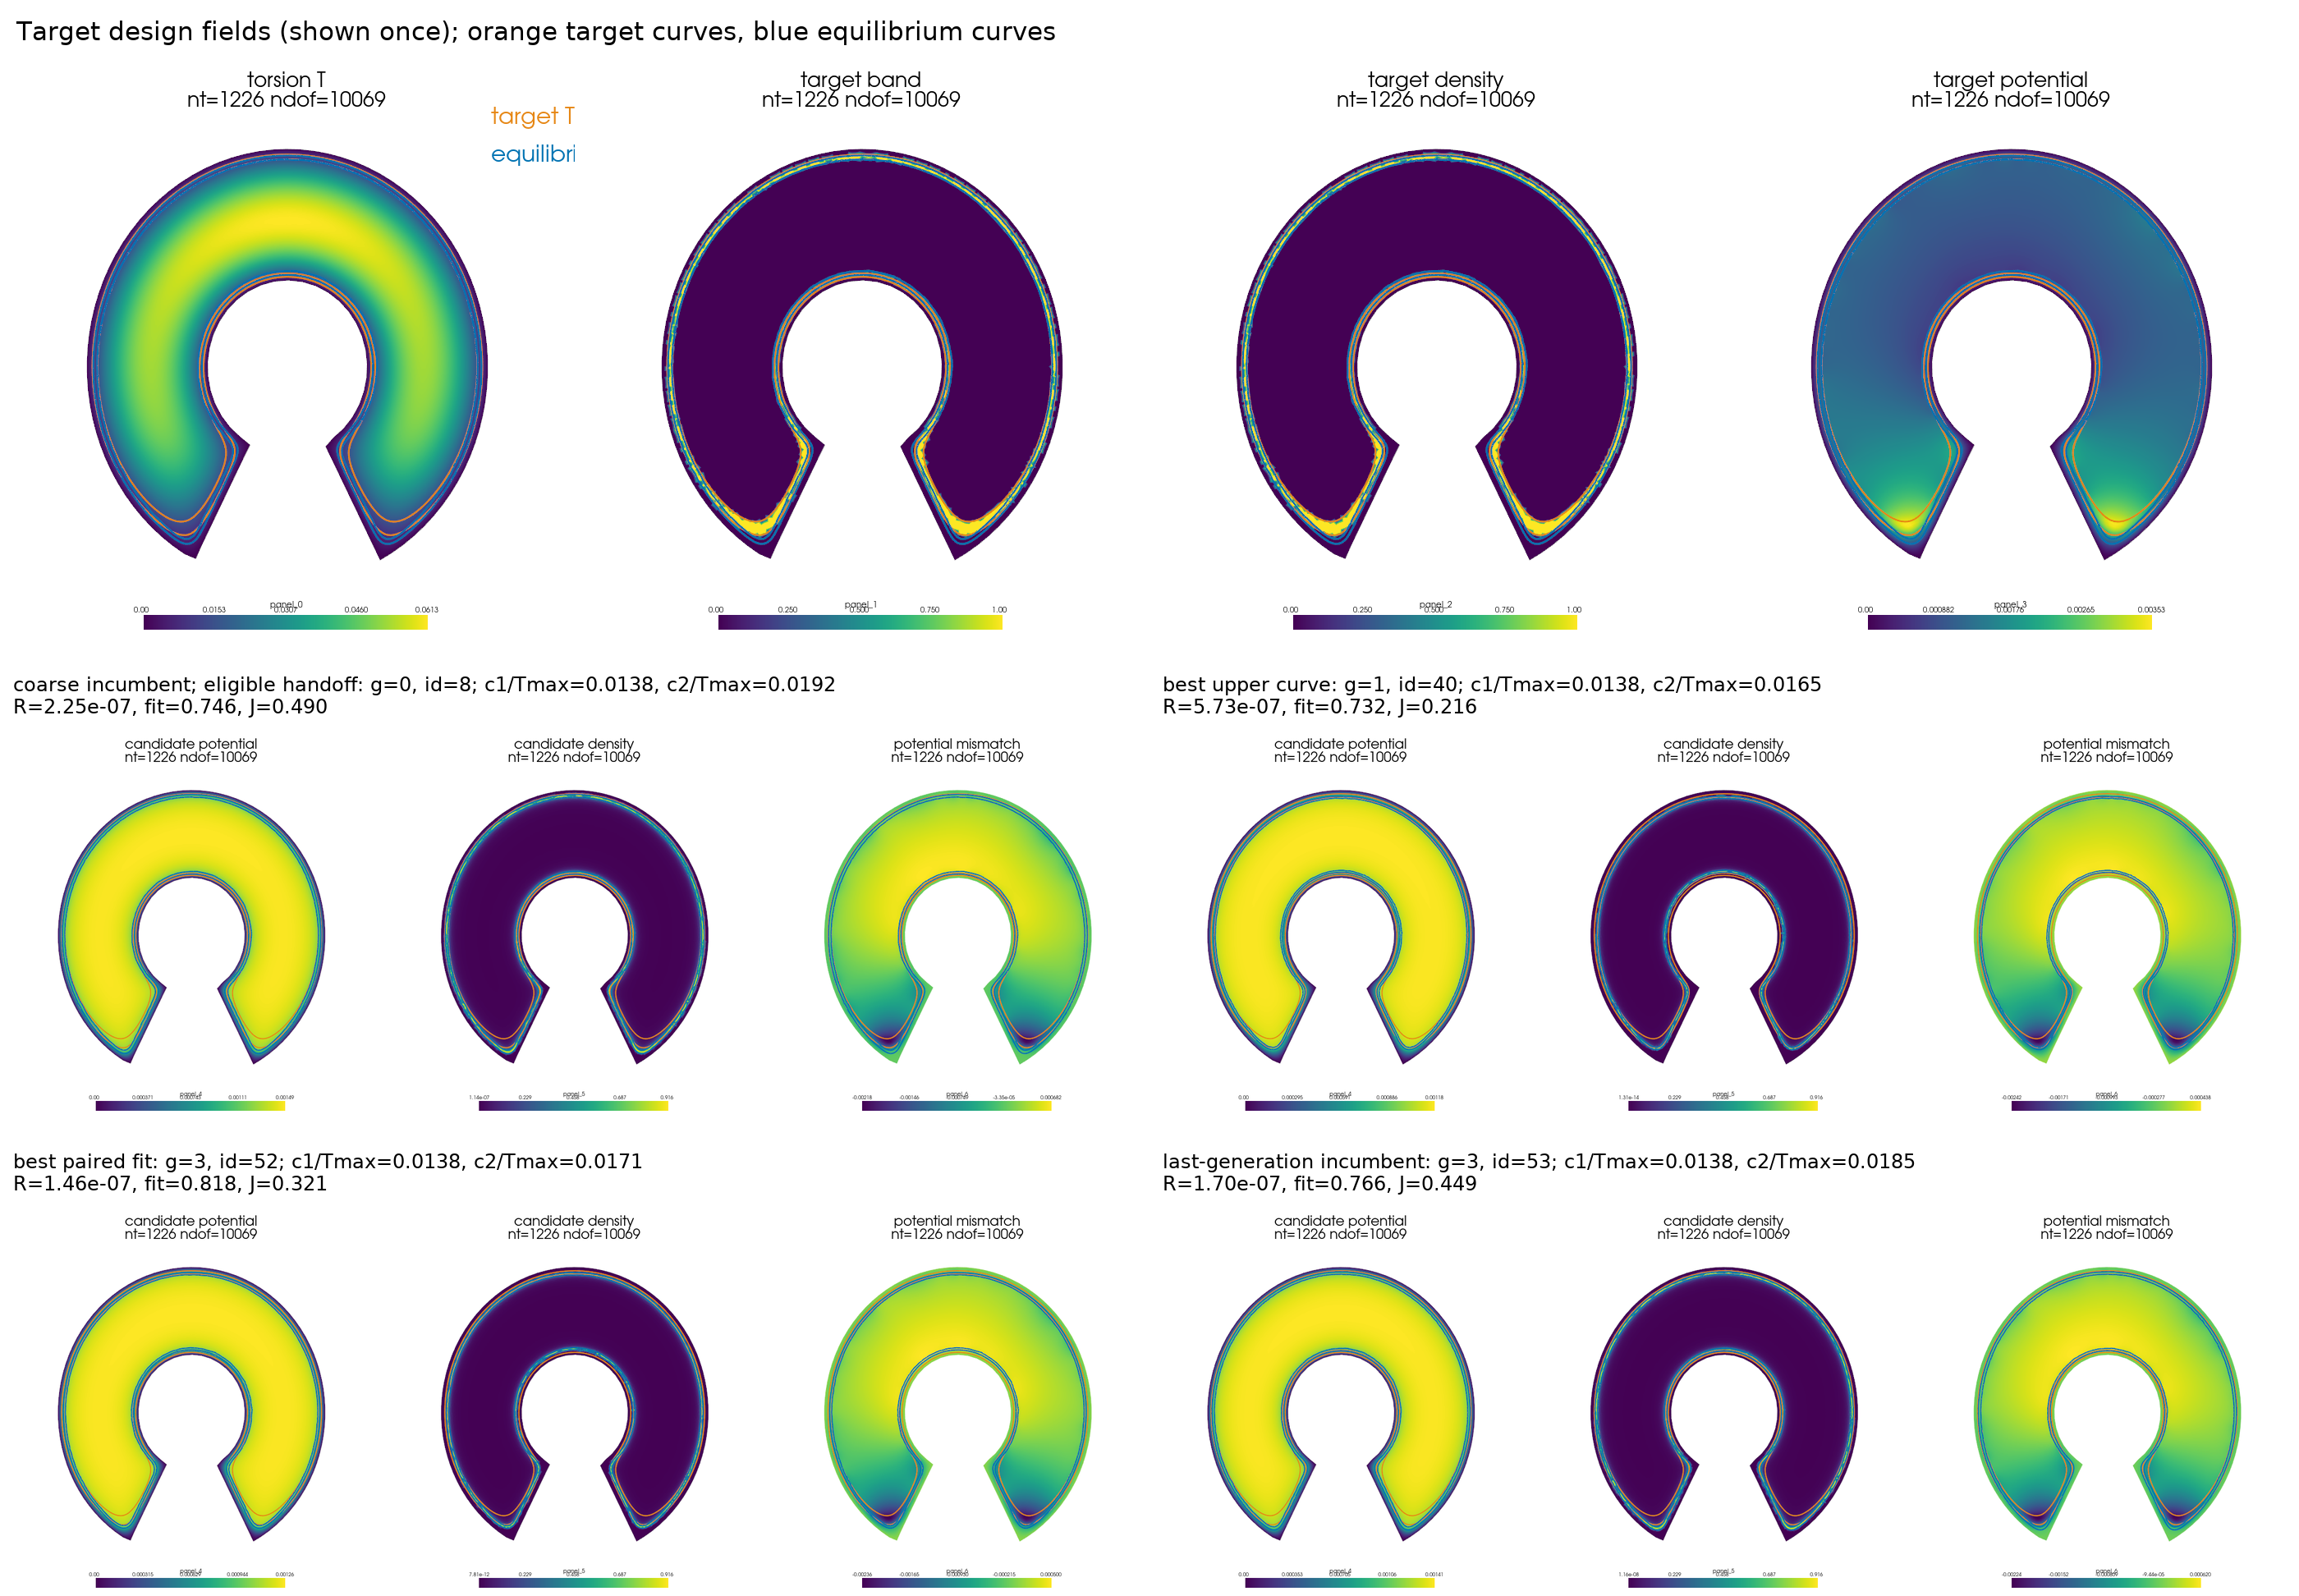
\includegraphics[width=0.49\linewidth]{figures/horseshoe_0p14_0p255_adaptive_continuation_epsratio0160_candidate_storyboard.png}
\caption{Design-once candidate storyboards for Pacman (left) and horseshoe
(right).  Target fields are separated from candidate rows; orange dashed
torsion-band contours and blue solid equilibrium contours use complete
rank-zero-gathered fields, and mesh edges are hidden.  The portable bundle
also contains all 109 and 54 individual candidate PNGs in 28 and 14 contact
sheets.  Data status: actual.}
\label{fig:adaptive-pacman-horseshoe-candidates}
\end{figure}
\end{landscape}

\begin{landscape}
\begin{figure}[tbp]
\centering
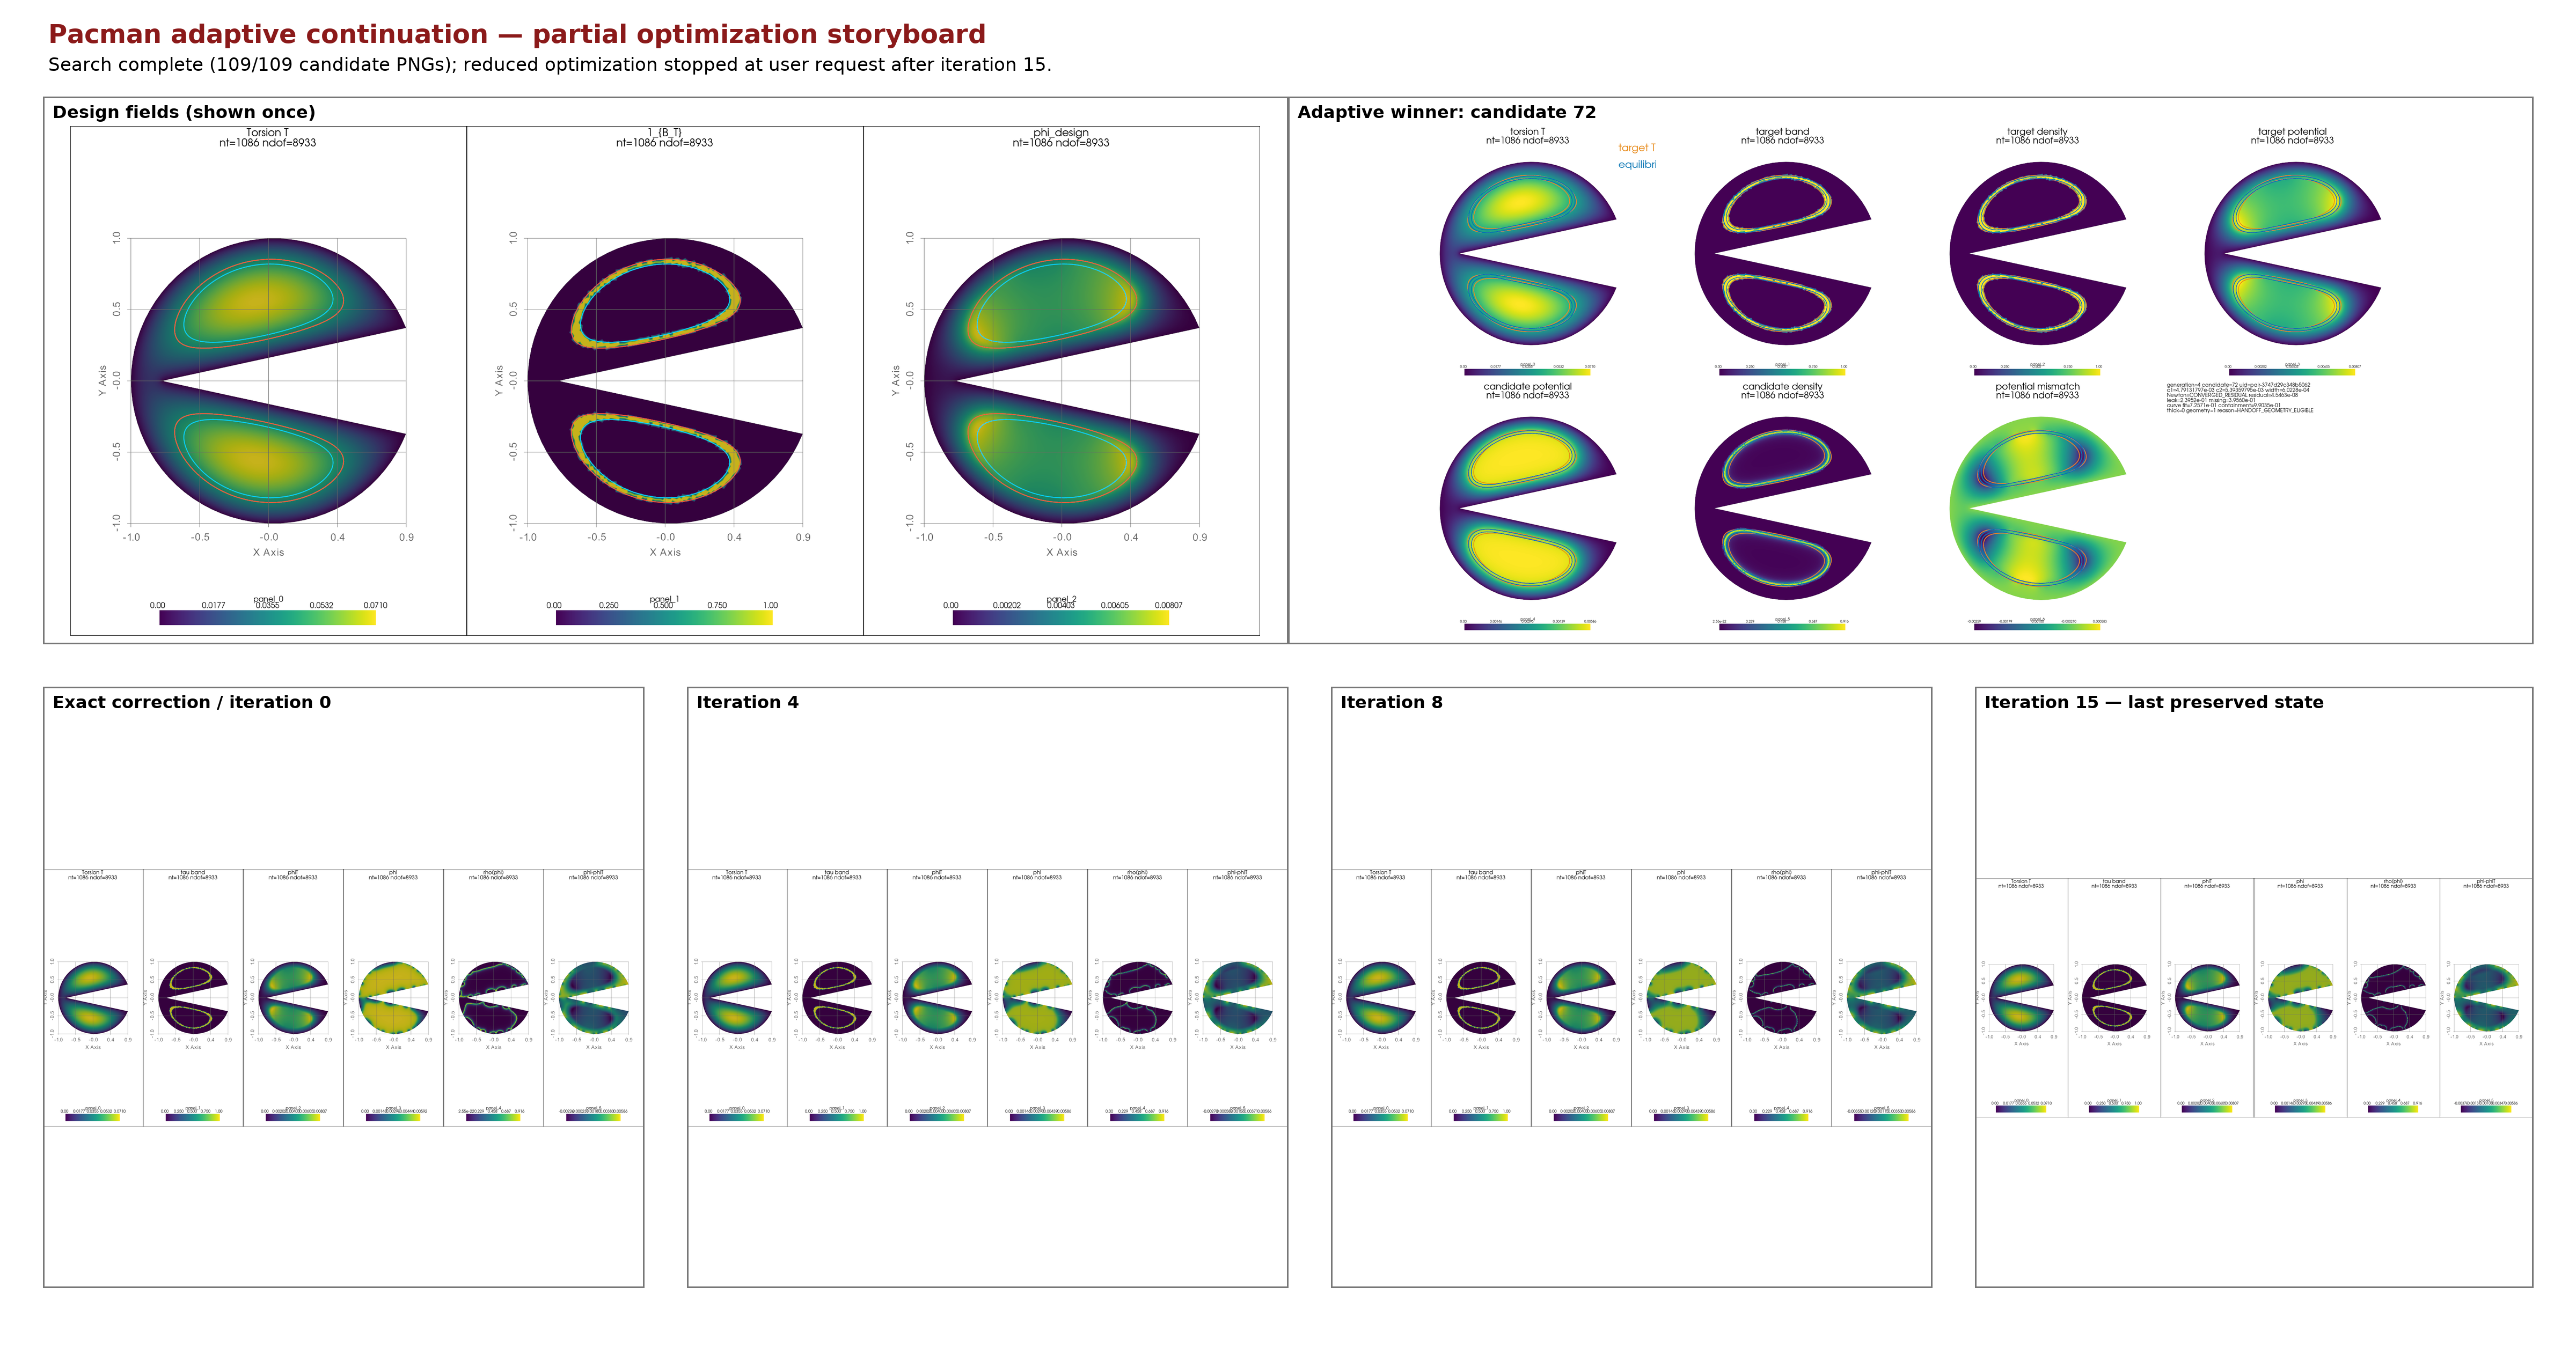
\includegraphics[width=0.49\linewidth]{figures/pacman_0p55_0p645_adaptive_continuation_epsratio0160_partial_storyboard.png}
\hfill
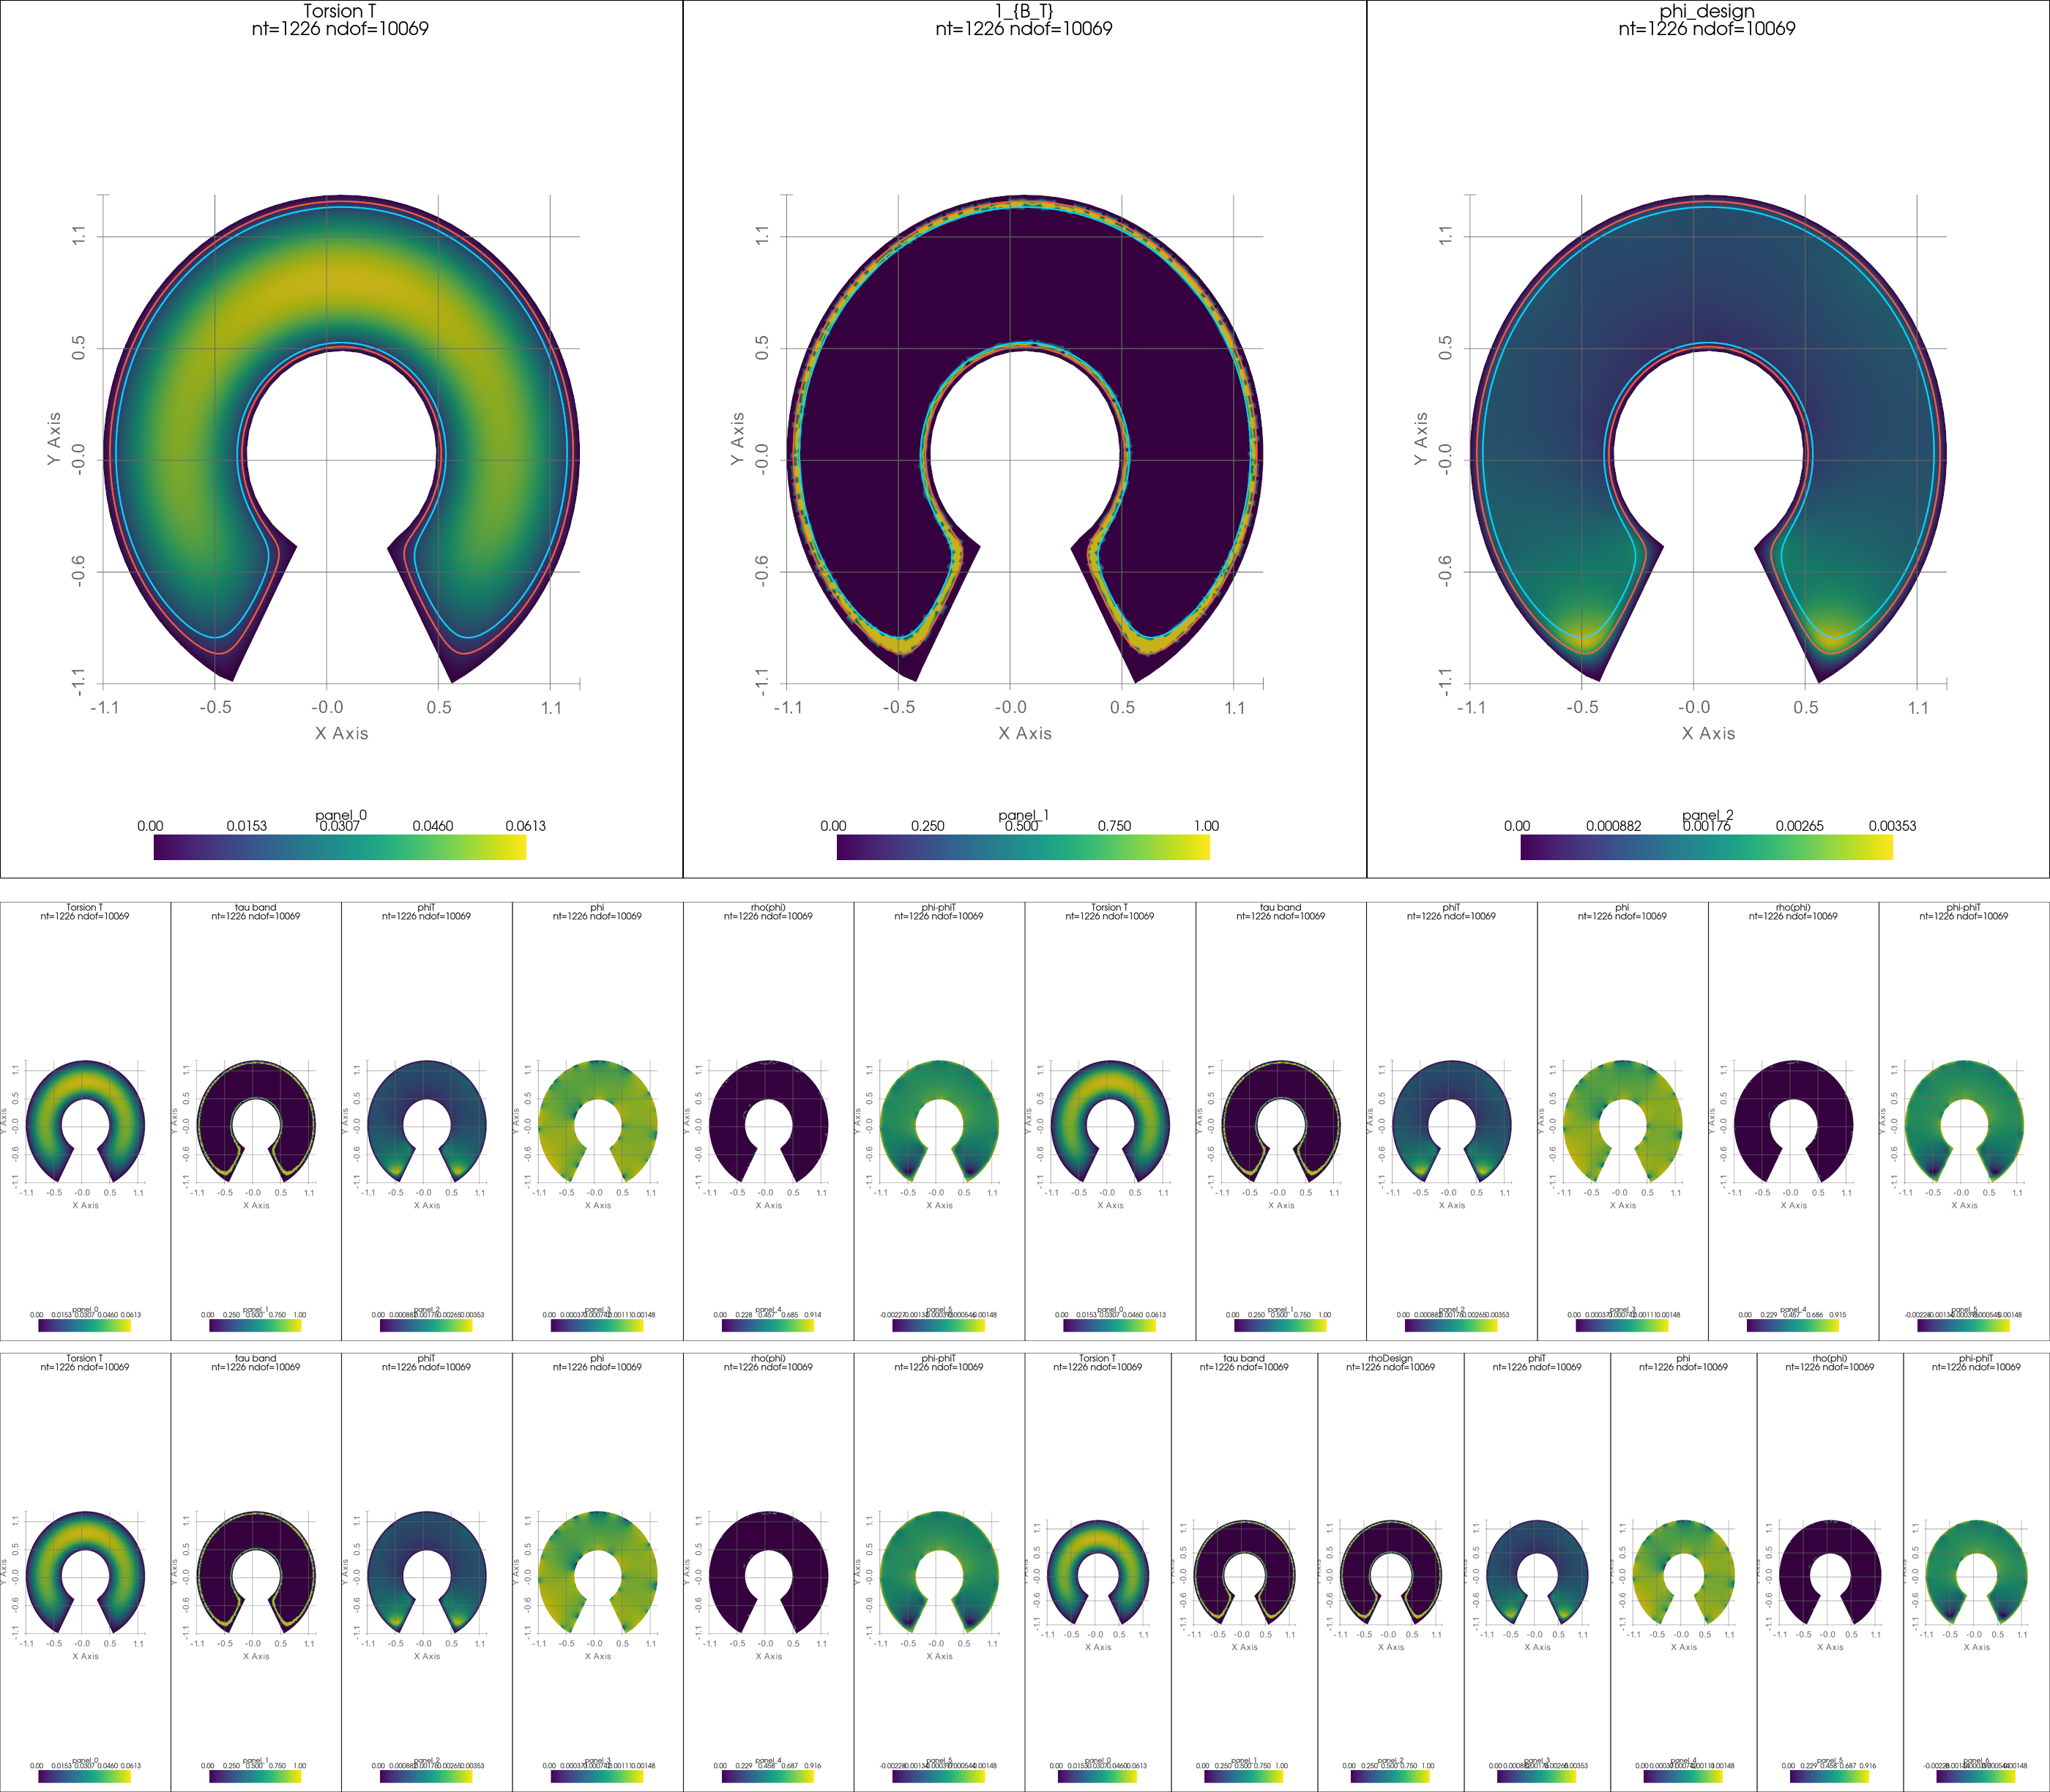
\includegraphics[width=0.49\linewidth]{figures/horseshoe_0p14_0p255_adaptive_continuation_epsratio0160_storyboard.png}
\caption{Reduced-optimization evolution after adaptive handoff: the explicitly
partial Pacman sequence through iteration 15 (left) and the terminal
horseshoe sequence (right).  The design fields appear once, after which each
iteration retains only the evolving fields and both contour families.  The
panels document failure rather than hiding it: neither sequence yields an
area-matched equilibrium band.  Data status: actual.}
\label{fig:adaptive-pacman-horseshoe-storyboards}
\end{figure}
\end{landscape}

\subsection{Smoothing continuation on a wider, more interior horseshoe band}
\label{sec:horseshoe-interior-epsilon-continuation}

The preceding horseshoe target was both thin and close to the wall.  To
separate that geometric difficulty from nonlinear regularity, the adaptive
search was repeated on the wider, more interior band
$[\alpha_{T1},\alpha_{T2}]=[0.35,0.50]$.  No threshold pair was supplied:
each search again covered the complete physical triangle
$0\leq c_{1,\phi}<c_{2,\phi}\leq\max T$.  The $P_4$, $h=0.075$ mesh has
$1{,}226$ cells and $10{,}069$ global degrees of freedom.  Twenty independent
one-rank MUMPS groups solved and rendered the candidates, and a four-rank
MUMPS solve handled the reduced-optimization handoff.  The torsion indicator
was sharp, while the equilibrium smoothing ratio was continued through
$0.08$, $0.12$, and $0.16$.

Table~\ref{tab:horseshoe-interior-epsilon-continuation} gives the controlled
comparison.  The most-contained entry refers to the candidate maximizing paired
level-curve containment among bounded candidates with both curves active; its
Jaccard index and Newton residual are reported on the same row.  At ratios
$0.08$ and $0.12$, the most geometrically relevant candidates stalled near
$2.7\times10^{-3}$ and $2.4\times10^{-3}$, so neither search produced a
handoff.  Raising the ratio to $0.16$ regularized the candidate solves: 26 of
157 pairs passed the loose PDE/geometric handoff gate.  None passed the strict
mesh-resolution gate, so the outcome must not be described as fully
certified.  All 481 solved candidates, including failed and partial solves,
have individual rank-zero-gathered PNGs; the portable bundle also contains
122 four-candidate contact sheets.

\begin{table}[tbp]
\centering
\caption{Geometry-independent smoothing continuation for the horseshoe target
band $[0.35,0.50]$.  The candidate Newton tolerance is $10^{-6}$.  Data
status: actual.}
\label{tab:horseshoe-interior-epsilon-continuation}
\begin{tabular}{rrrrrrrr}
\toprule
$\varepsilon_\phi/\Delta c_\phi$ & Solved & PDE gate & Loose & Strict &
Containment & Jaccard & Residual \\
\midrule
0.08 & 162 & 126 & 0  & 0 & 0.72519 & 0.16902 & $2.683\times10^{-3}$ \\
0.12 & 162 & 120 & 0  & 0 & 0.71428 & 0.14668 & $2.441\times10^{-3}$ \\
0.16 & 157 & 121 & 26 & 0 & 0.96735 & 0.46195 & $5.144\times10^{-8}$ \\
\bottomrule
\end{tabular}
\end{table}

\begin{landscape}
\begin{figure}[tbp]
\centering
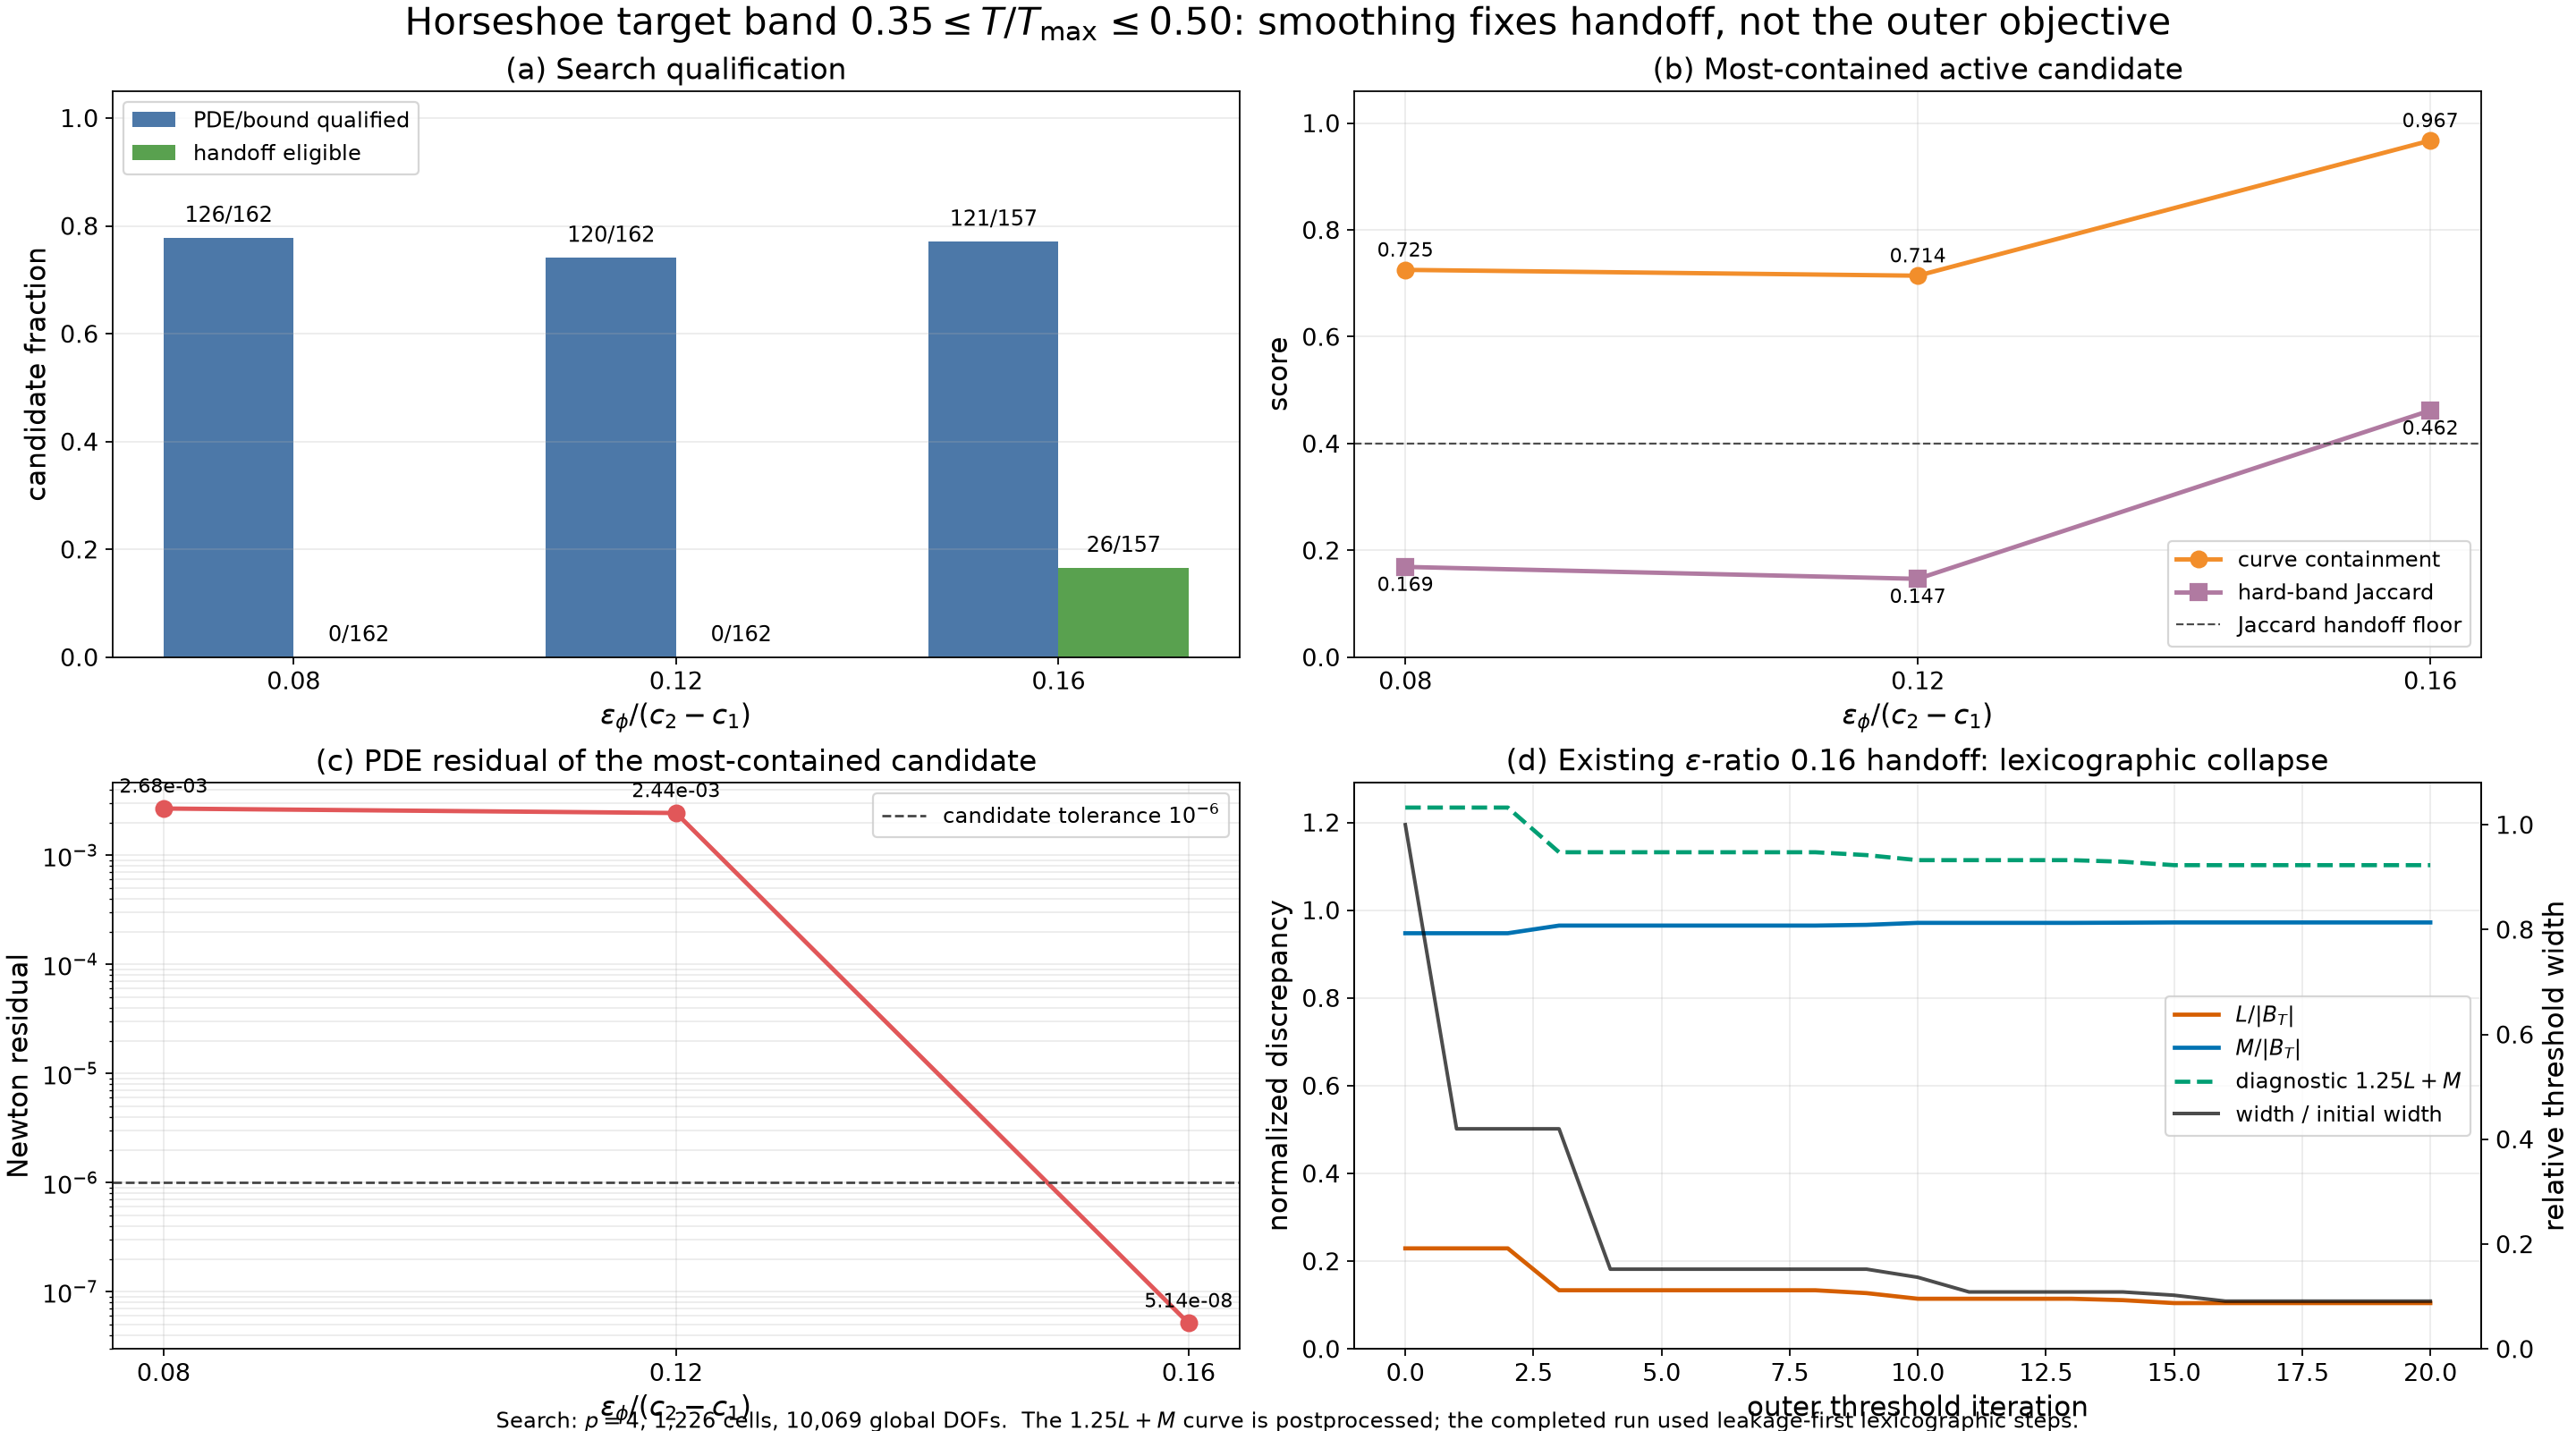
\includegraphics[width=0.96\linewidth,height=0.77\textheight,keepaspectratio]{figures/horseshoe_0p35_0p50_epsilon_continuation_comparison.png}
\caption{Horseshoe smoothing continuation.  Panels (a)--(c) show that
$\varepsilon_\phi/\Delta c_\phi=0.16$ resolves the adaptive-search handoff,
whereas $0.08$ and $0.12$ do not.  Panel (d) then isolates a distinct outer
optimization failure: the completed run used the leakage-first lexicographic
rule, which reduces leakage while collapsing the threshold width and
increasing missing area.  The dashed $1.25L+M$ curve is diagnostic
postprocessing, not the objective used by this completed run.  Data status:
actual.}
\label{fig:horseshoe-interior-epsilon-continuation}
\end{figure}
\end{landscape}

The selected $0.16$ search state is candidate 93, with
$(c_{1,\phi},c_{2,\phi})=(0.00305315,0.00375638)$, search residual
$5.144\times10^{-8}$, paired containment $0.96735$, hard-band Jaccard index
$0.46195$, and relative leakage/missing area $(0.35162,0.48244)$.  An exact
correction of this saved state reaches residual $6.326\times10^{-16}$.
Finite-difference checks at step fractions $10^{-3}$ and $3\times10^{-4}$
verify both sensitivity columns: the state-derivative relative $L^2$ errors
decrease from $2.53\times10^{-7}$ and $1.21\times10^{-7}$ to
$2.27\times10^{-8}$ and $1.09\times10^{-8}$, respectively.  The corresponding
relative leakage-gradient errors decrease from $5.23\times10^{-7}$ and
$1.44\times10^{-7}$ to $4.71\times10^{-8}$ and $1.30\times10^{-8}$.
Consequently, this experiment provides no evidence of a sensitivity-sign or
threshold-derivative bug.

\begin{landscape}
\begin{figure}[tbp]
\centering
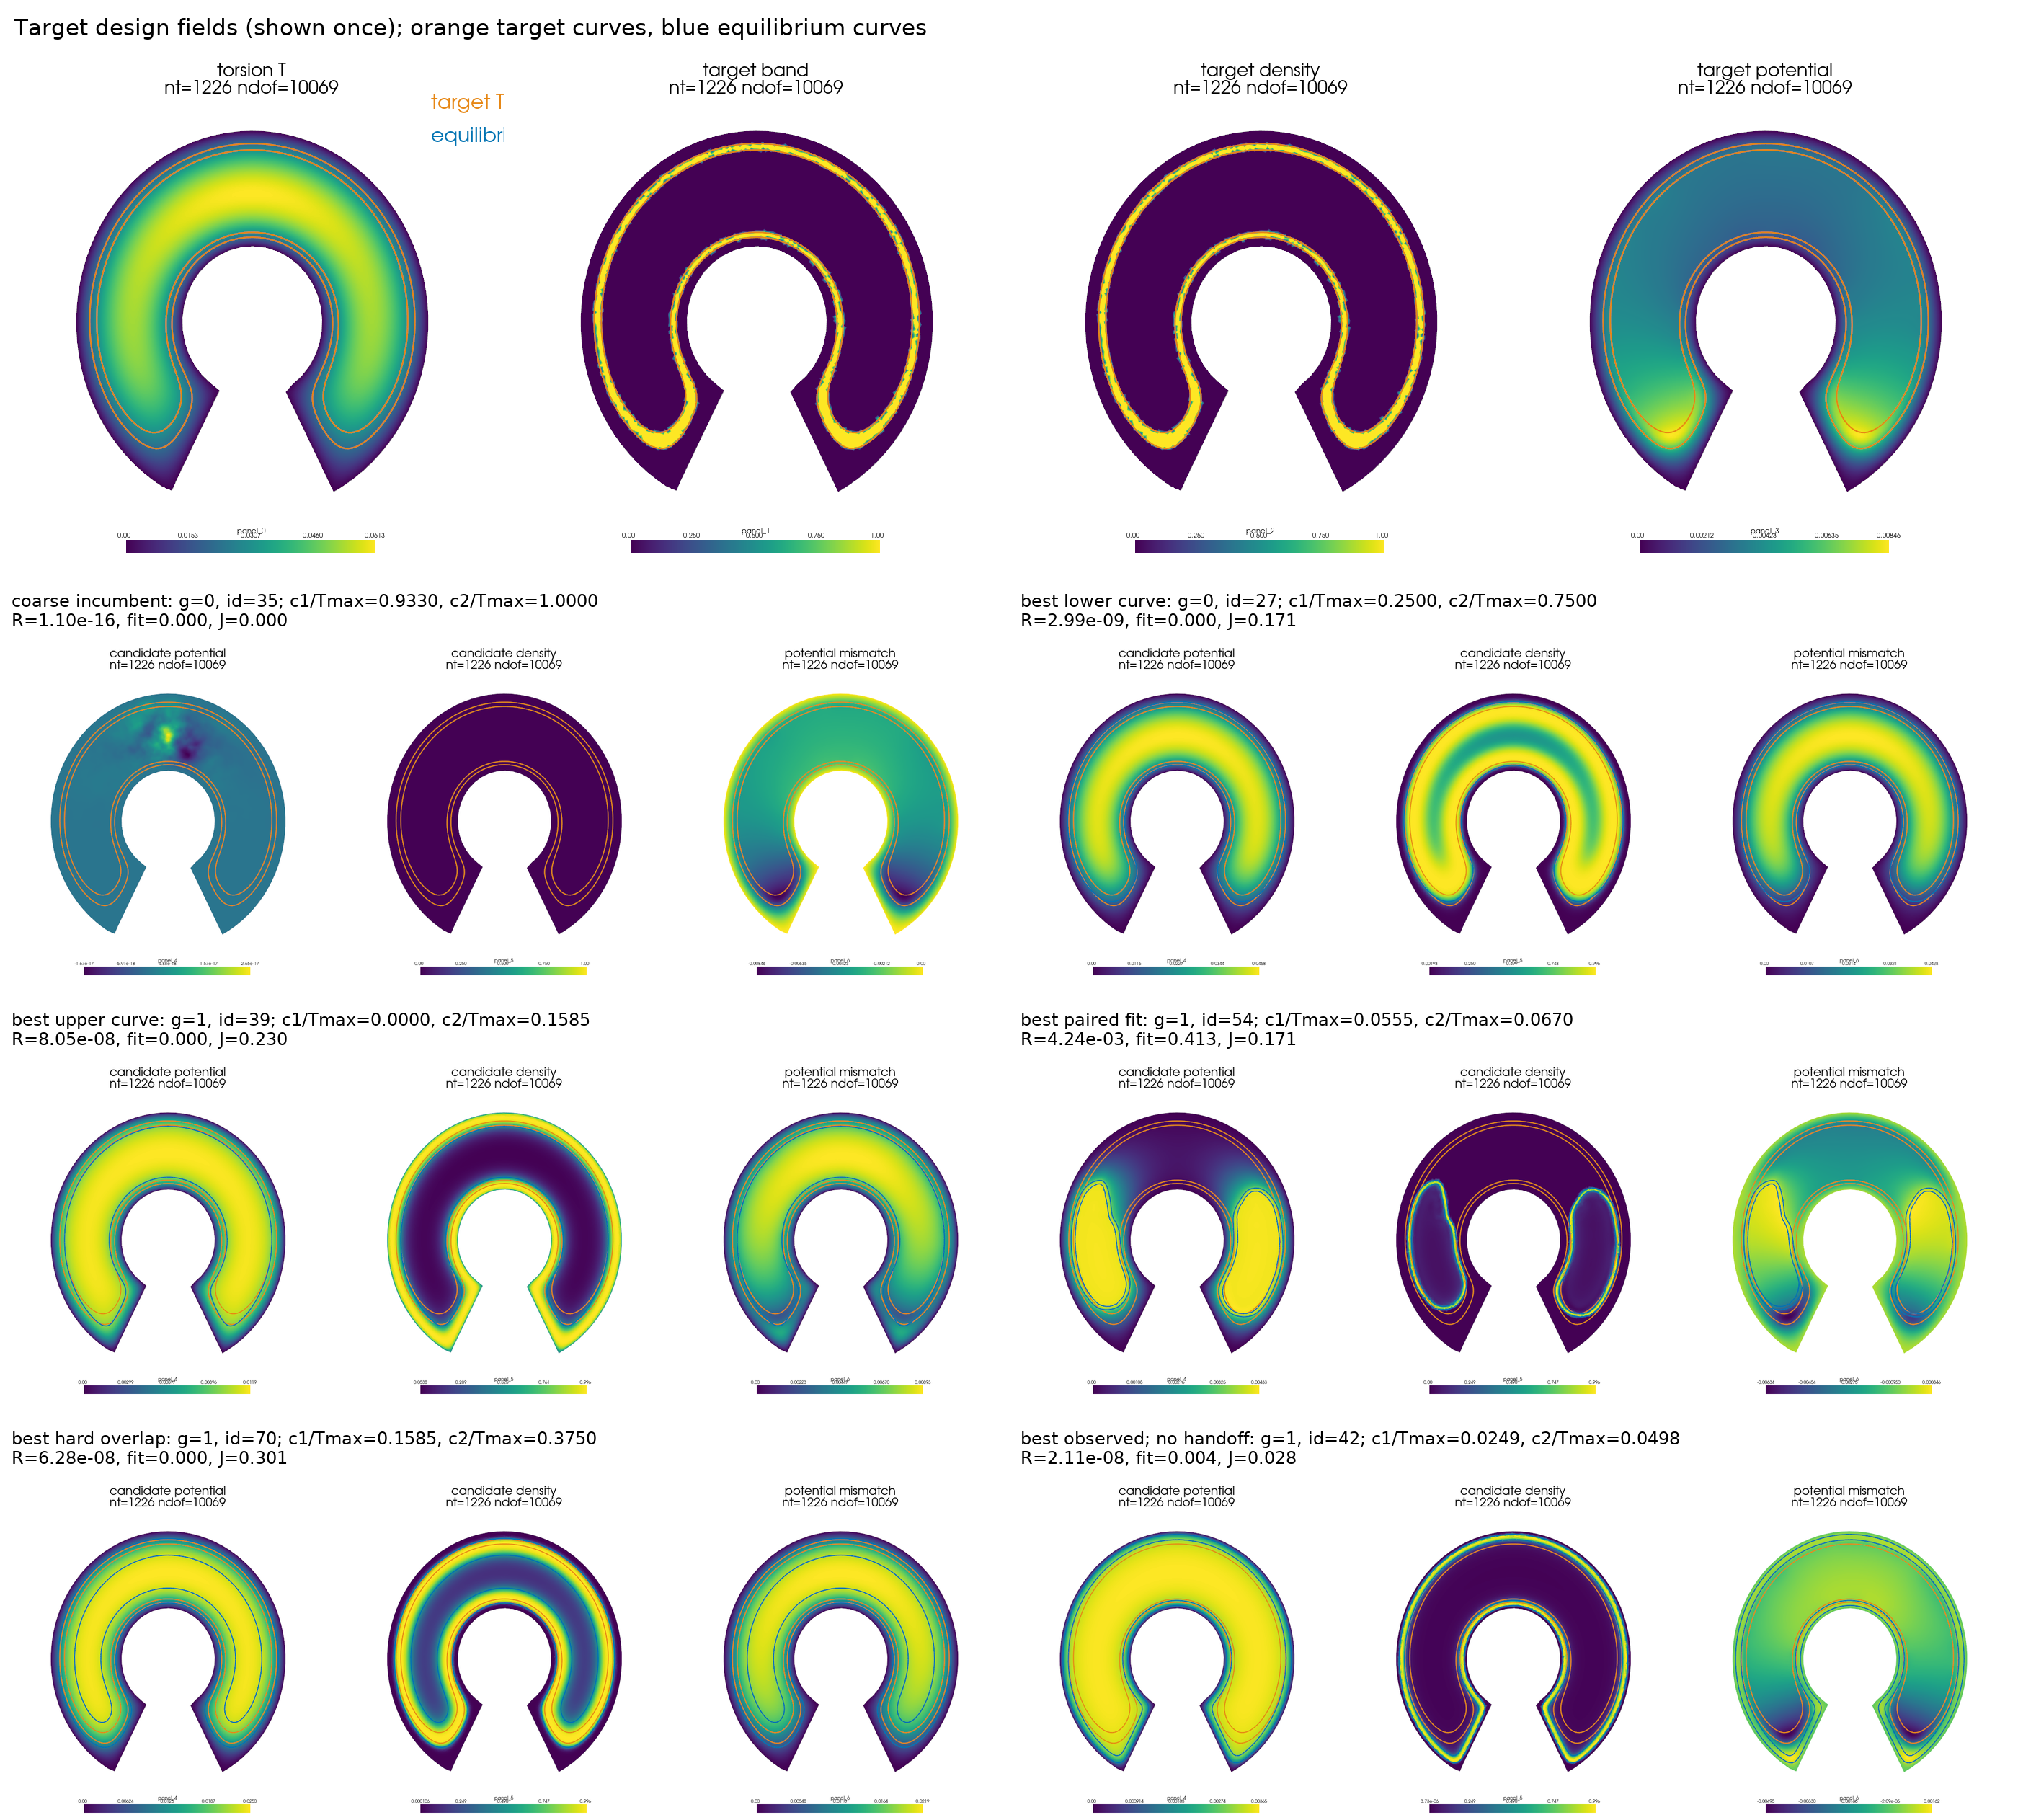
\includegraphics[width=0.48\linewidth,height=0.75\textheight,keepaspectratio]{figures/horseshoe_0p35_0p50_adaptive_continuation_epsratio0080_candidate_storyboard.png}
\hfill
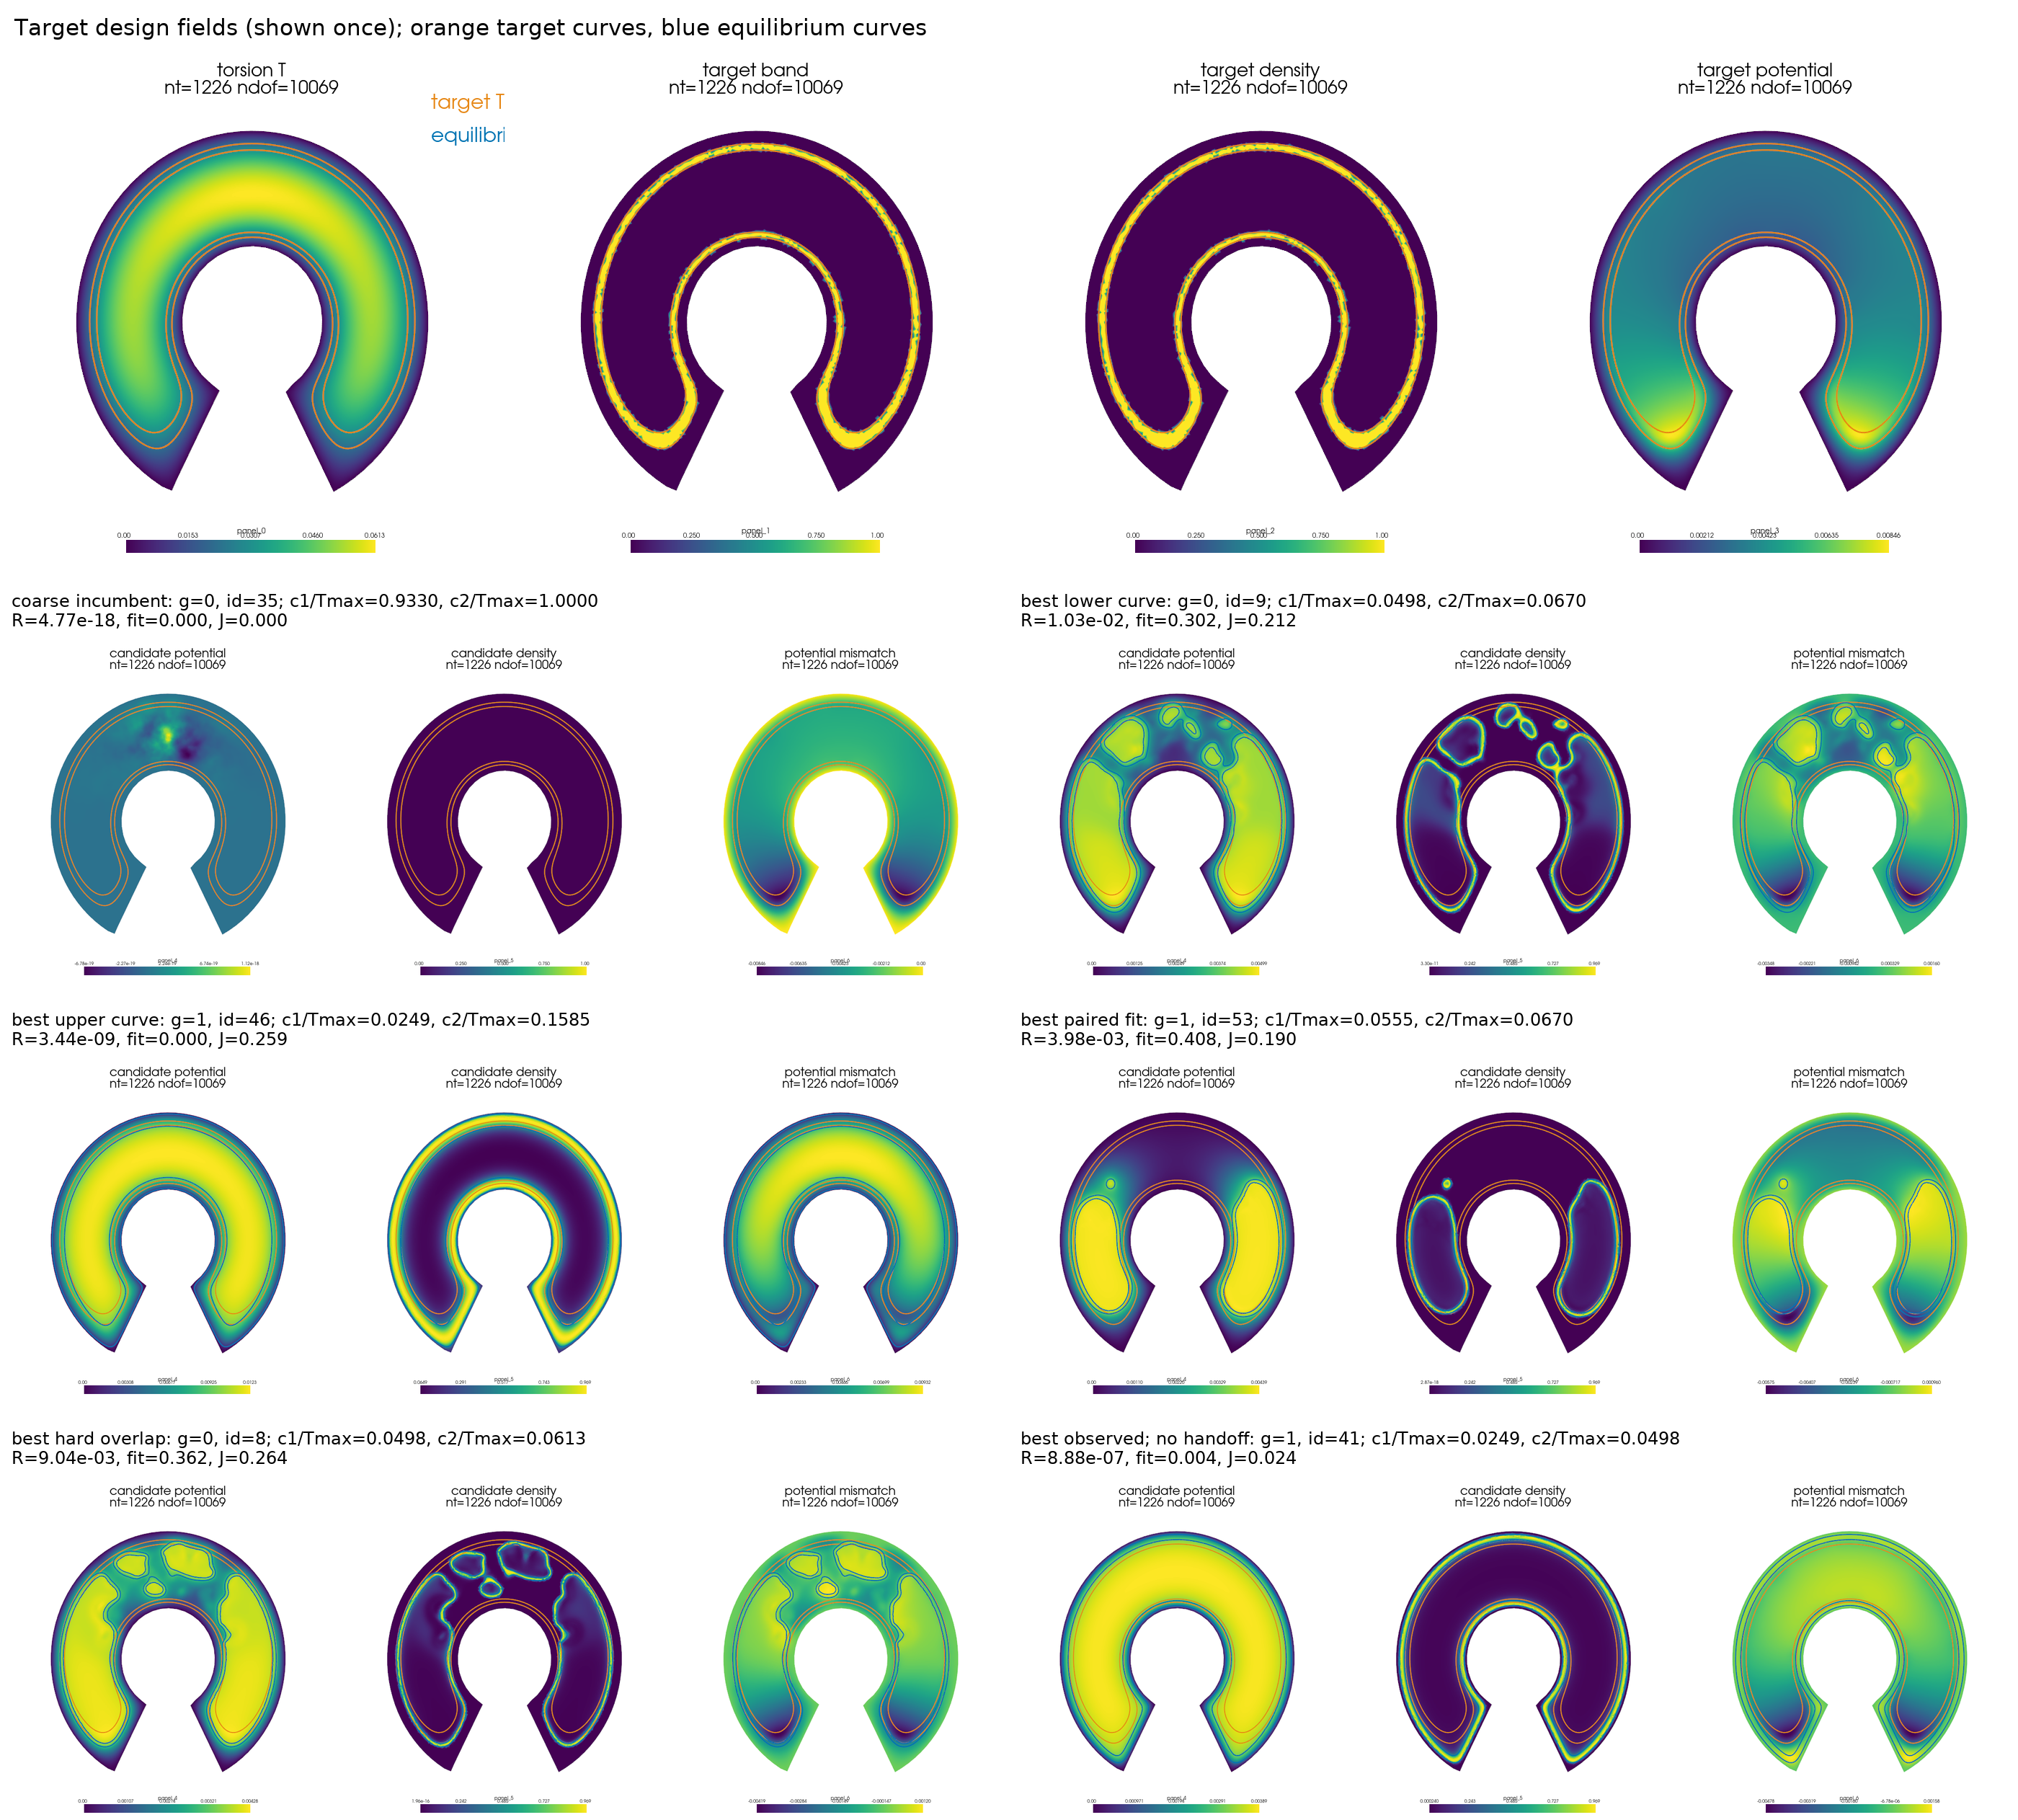
\includegraphics[width=0.48\linewidth,height=0.75\textheight,keepaspectratio]{figures/horseshoe_0p35_0p50_adaptive_continuation_epsratio0120_candidate_storyboard.png}
\caption{Design-once candidate storyboards for the failed $0.08$ (left) and
$0.12$ (right) smoothing searches.  The failure panels are retained rather
than discarded: both contain promising geometric states, but their Newton
residuals remain far above the $10^{-6}$ candidate gate.  Every field is
assembled from a complete rank-zero gather, orange dashed contours are fixed
torsion-band boundaries, blue solid contours are candidate equilibrium
boundaries, and mesh edges are hidden.  Data status: actual; no handoff.}
\label{fig:horseshoe-interior-failed-search-storyboards}
\end{figure}
\end{landscape}

\begin{landscape}
\begin{figure}[tbp]
\centering
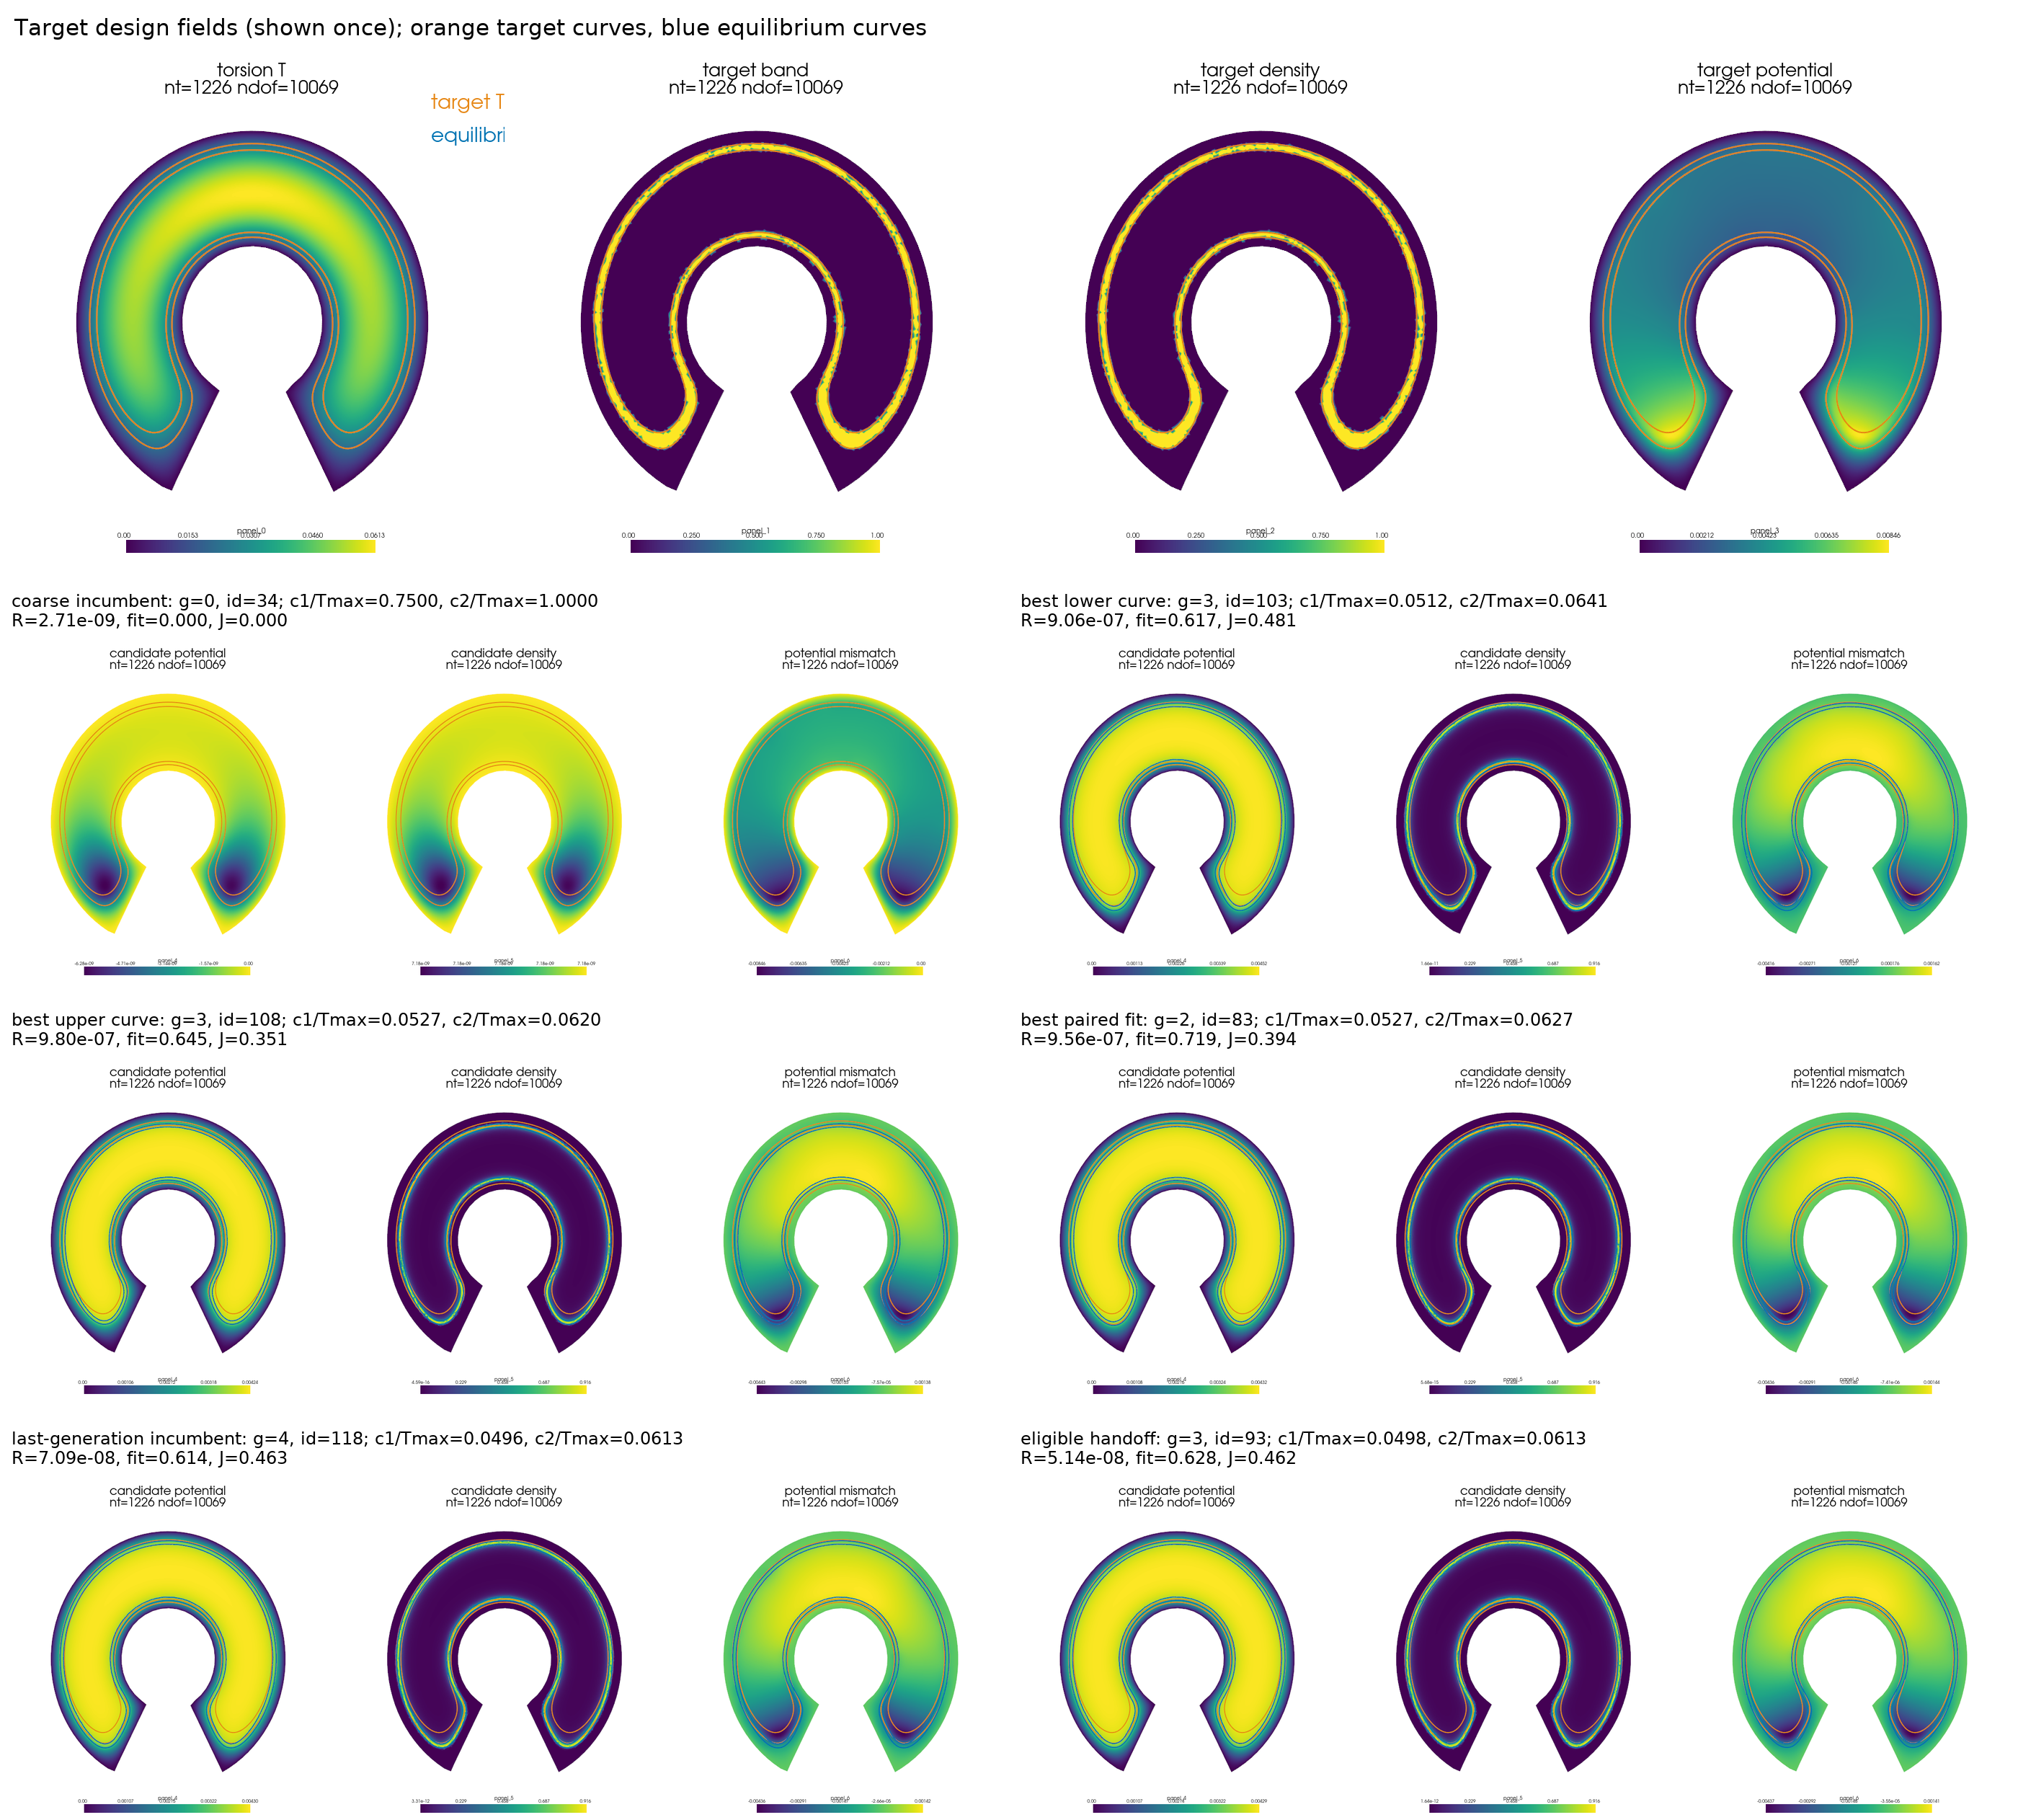
\includegraphics[width=0.48\linewidth,height=0.75\textheight,keepaspectratio]{figures/horseshoe_0p35_0p50_adaptive_continuation_epsratio0160_candidate_storyboard.png}
\hfill
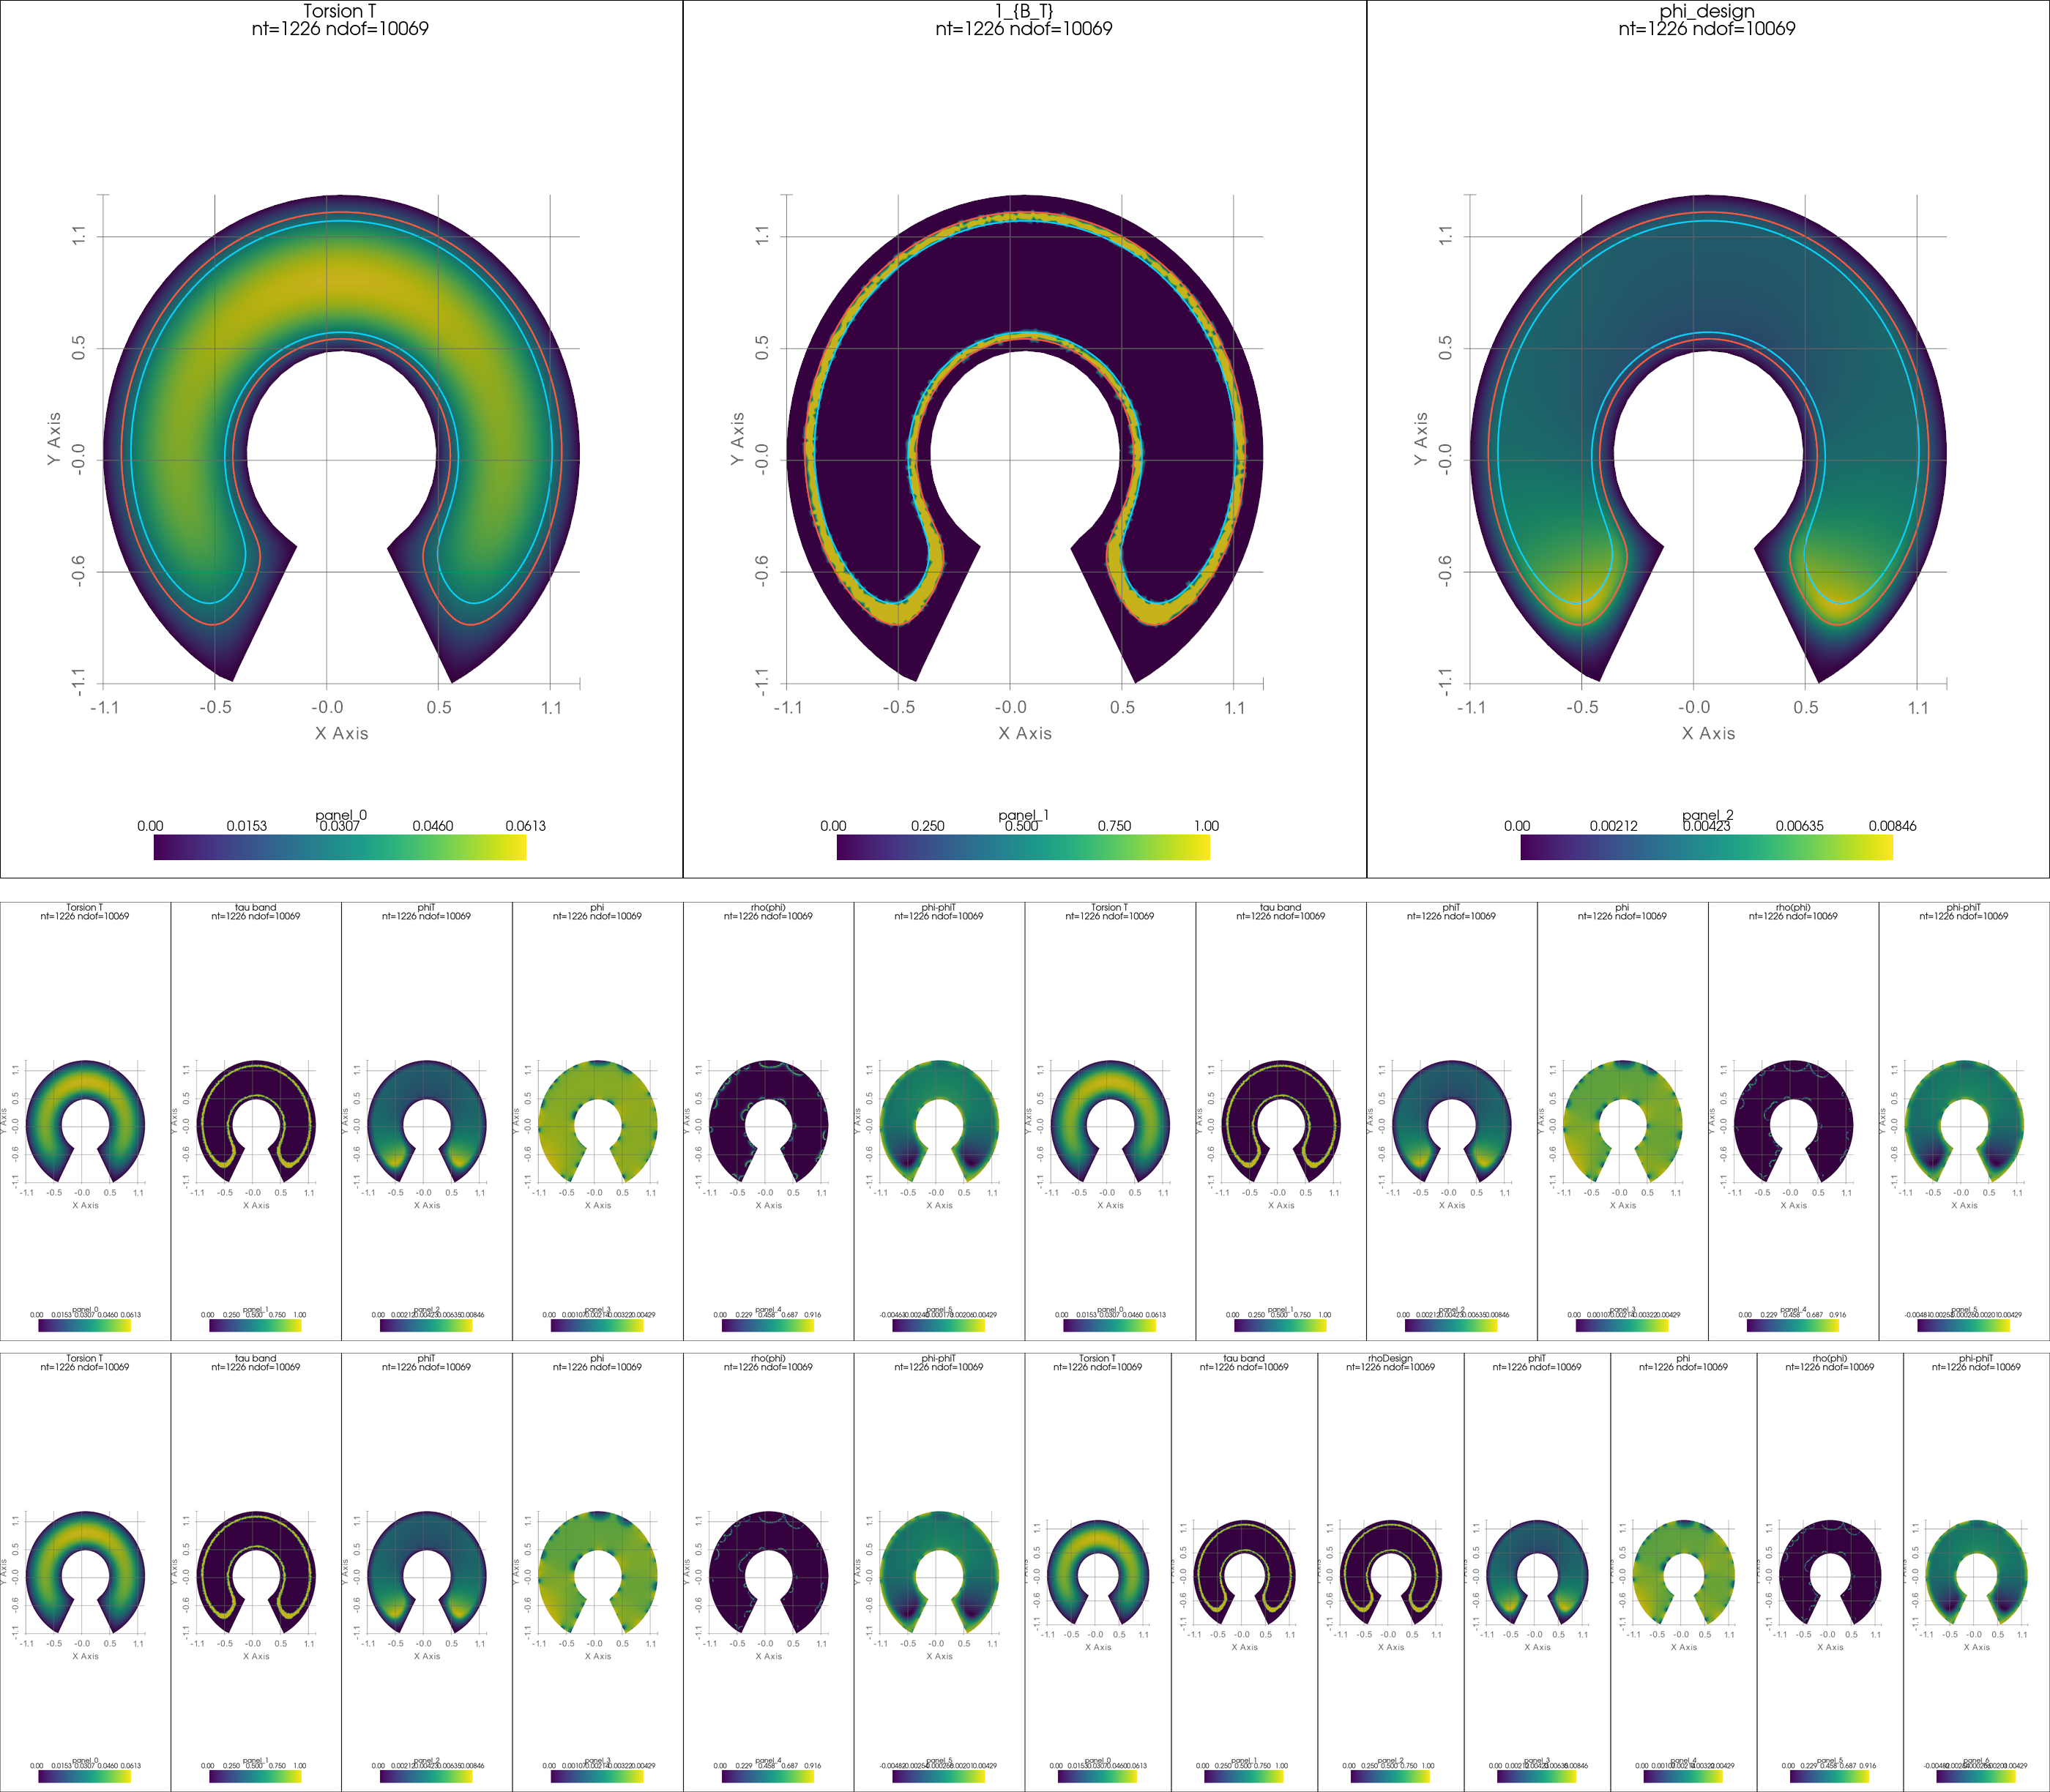
\includegraphics[width=0.48\linewidth,height=0.75\textheight,keepaspectratio]{figures/horseshoe_0p35_0p50_adaptive_continuation_epsratio0160_storyboard.png}
\caption{Successful adaptive handoff at smoothing ratio $0.16$ (candidate
search, left) followed by the terminal reduced-optimization evolution (right).
The target/design fields are plotted once; subsequent rows retain the fixed
orange dashed target contours and moving blue equilibrium contours.  The
storyboard documents geometric failure: the outer iteration contracts the
window instead of filling the target band.  Data status: actual.}
\label{fig:horseshoe-interior-eps016-storyboards}
\end{figure}
\end{landscape}

The reduced optimizer accepts six steps before terminating with
\texttt{STEP\_TOO\_SMALL}.  It contracts
$c_{2,\phi}-c_{1,\phi}$ from $7.0323\times10^{-4}$ to
$6.4095\times10^{-5}$ while relative leakage falls to $0.10445$ and relative
missing area rises to $0.97194$; the final hard active-set Jaccard index is
$0.08689$.  The final residual $3.567\times10^{-11}$ is on the correct scale
but remains a factor $3.57$ above the requested general tolerance $10^{-11}$
and a factor $35.7$ above the final-projection tolerance $10^{-12}$.  This is
therefore an explicitly failed outer solve, not a PDE or geometric success.

Most importantly, the completed rule was not a \emph{slight} preference for
leakage: until leakage reached $0.02$, it was a lexicographic rule with
effectively infinite priority over missing area.  We therefore repeated the
full geometry-independent search and exact optimization with the finite merit
\[
  J_{1.25:1}=\frac{1.25L_{\rm rel}+M_{\rm rel}}{2.25},
\]
while retaining the PDE, branch-overlap, activity, threshold-bound, and
minimum-width guards.  No threshold pair or favourable neighbourhood was
supplied to the search.  Its 20 MPI workers evaluated 157 candidates, all of
which were gathered and rendered by rank zero; the same candidate passed the
handoff gates as in the original $\varepsilon_\phi/\Delta c_\phi=0.16$ run.

The exact weighted optimization reached a final PDE residual of
$1.519\times10^{-15}$, so this retry decisively rules out nonlinear-solve
accuracy as the terminal failure.  Nevertheless, six accepted steps again
contracted the threshold interval to the imposed minimum width
$6.132\times10^{-5}$.  At termination, $L_{\rm rel}=0.09387$,
$M_{\rm rel}=0.97473$, and the hard active-set Jaccard index was only
$0.08372$.  The run is therefore classified as PDE-converged but geometrically
failed (\texttt{STEP\_TOO\_SMALL}); it is retained in every diagnostic rather
than being filtered from the study.

\begin{table}[htbp]
\centering
\caption{Exact outer-optimization outcomes for the two leakage/missing-area
policies.  Both start from independently generated adaptive-search handoffs.
The finite merit shown for the lexicographic run is evaluated afterward using
the same $1.25{:}1$ weights, to permit a common comparison.}
\label{tab:horseshoe-objective-policy}
\begin{tabular}{lrrrrrl}
\toprule
Policy & PDE residual & $\Delta c_\phi$ & $L_{\rm rel}$ & $M_{\rm rel}$ & Jaccard & Outcome \\
\midrule
Lexicographic & $3.567\times10^{-11}$ & $6.410\times10^{-5}$ & 0.10445 & 0.97194 & 0.08689 & failed \\
Finite $1.25{:}1$ & $1.519\times10^{-15}$ & $6.132\times10^{-5}$ & 0.09387 & 0.97473 & 0.08372 & failed \\
\bottomrule
\end{tabular}
\end{table}

On the common finite scale, the weighted run reduced the merit from
$0.66145$ at its exact initial state to $0.48537$, compared with $0.49000$
for the lexicographic terminal state: an improvement of only about $0.9\%$.
Thus merely replacing infinite leakage priority by a modest finite preference
does not cure the collapse.  A nearly empty band can still trade a small
leakage reduction against almost complete target loss.  The result motivates
a coverage floor or barrier, a certified-area/Jaccard guard, or an explicit
Pareto acceptance rule, together with exact-branch recertification before
sensitivity-based steps; it does not justify further tuning of the scalar
weight on this case.

\begin{landscape}
\begin{figure}[p]
\centering
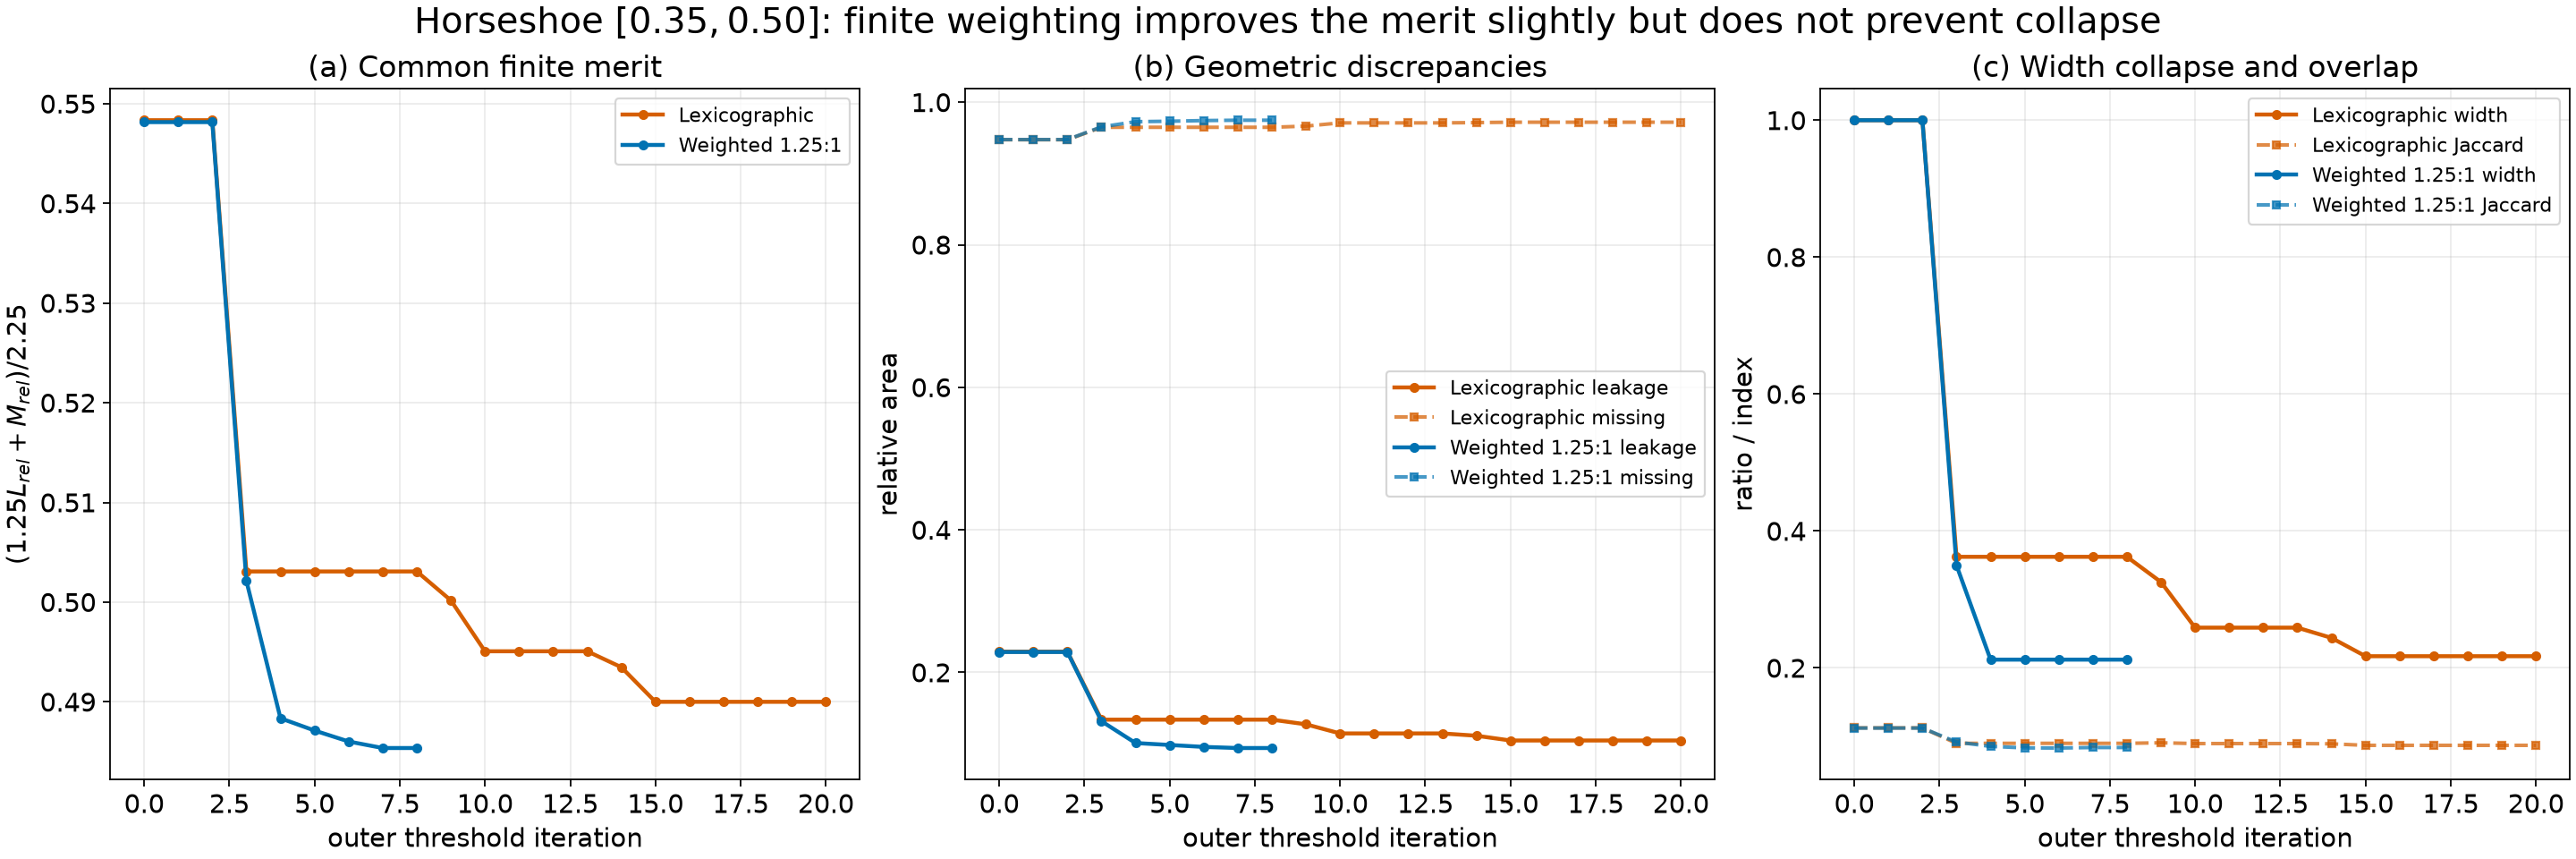
\includegraphics[width=0.98\linewidth]{figures/horseshoe_0p35_0p50_lexicographic_vs_weighted_objective.png}
\caption{Common-metric comparison of the original lexicographic policy and
the controlled finite $1.25{:}1$ leakage/missing-area policy.  The latter
solves the PDE to near machine precision but follows the same geometric
collapse, demonstrating that the remaining failure is in the scalar outer
objective and branch geometry rather than Newton tolerance.  Data status:
actual.}
\label{fig:horseshoe-objective-policy-comparison}
\end{figure}
\end{landscape}

\begin{landscape}
\begin{figure}[p]
\centering
\begin{minipage}[t]{0.49\linewidth}
\centering
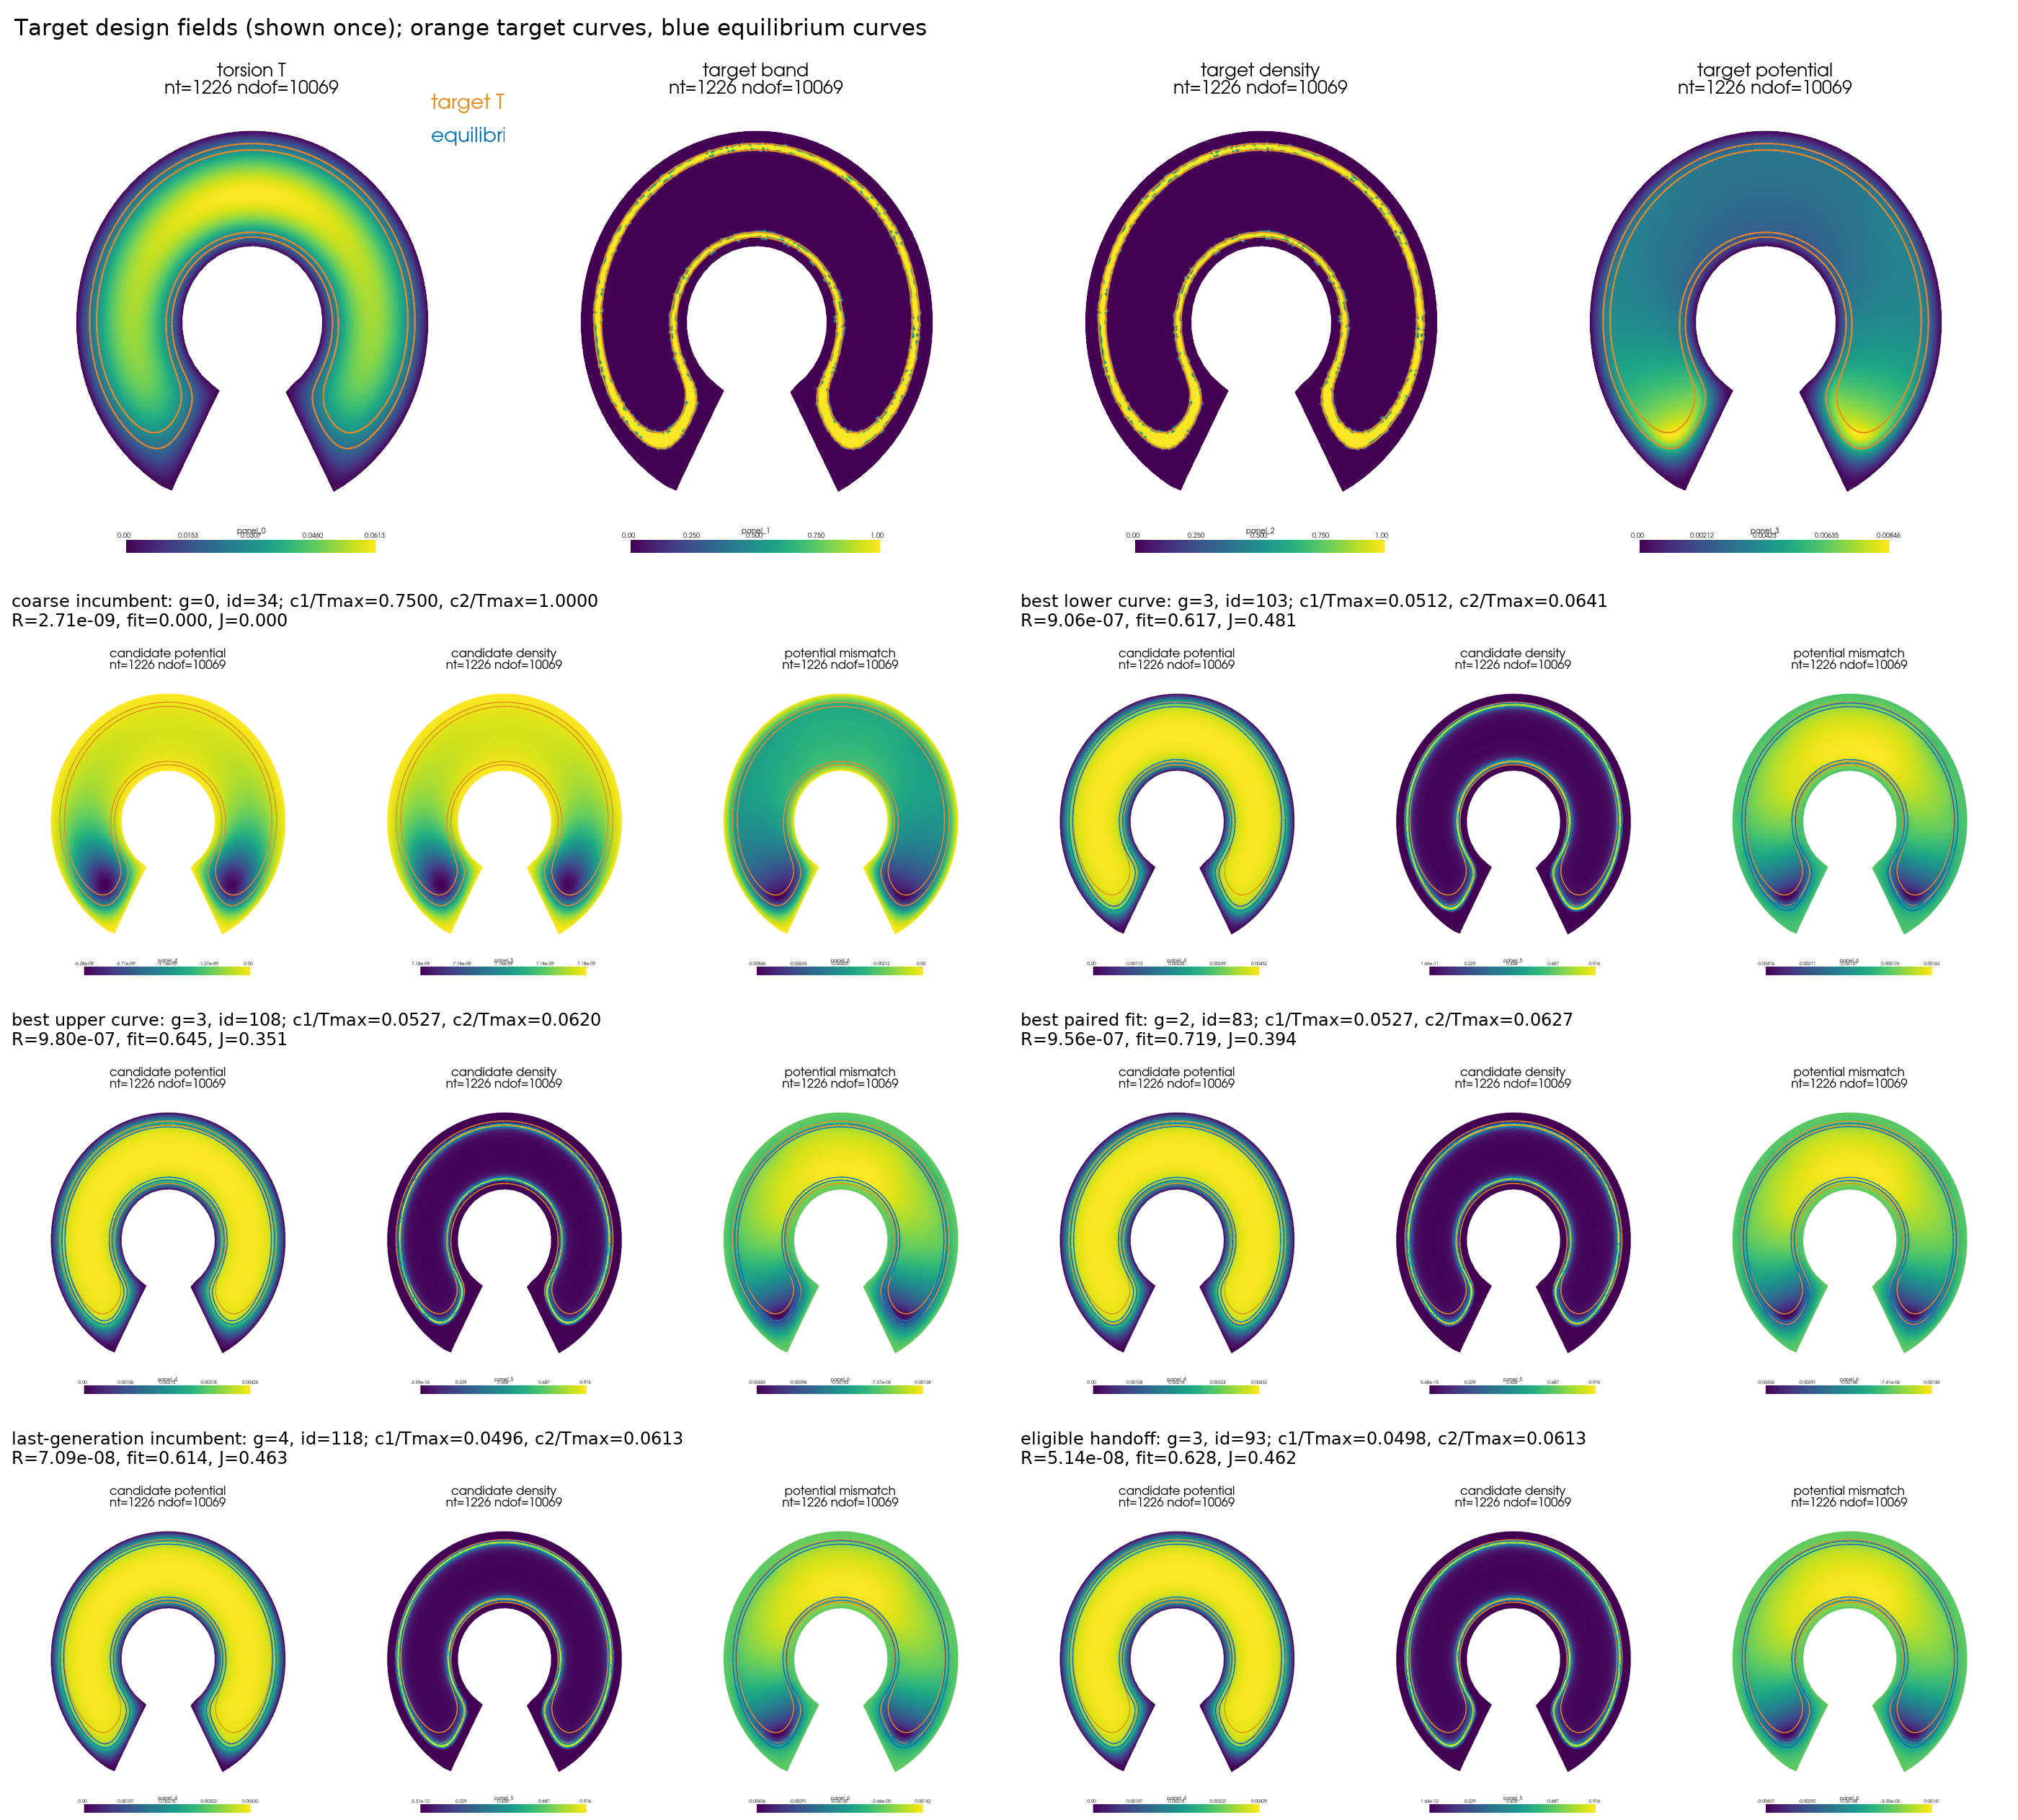
\includegraphics[width=\linewidth]{figures/horseshoe_0p35_0p50_adaptive_continuation_epsratio0160_weighted_l125_m100_candidate_storyboard.png}
\end{minipage}\hfill
\begin{minipage}[t]{0.49\linewidth}
\centering
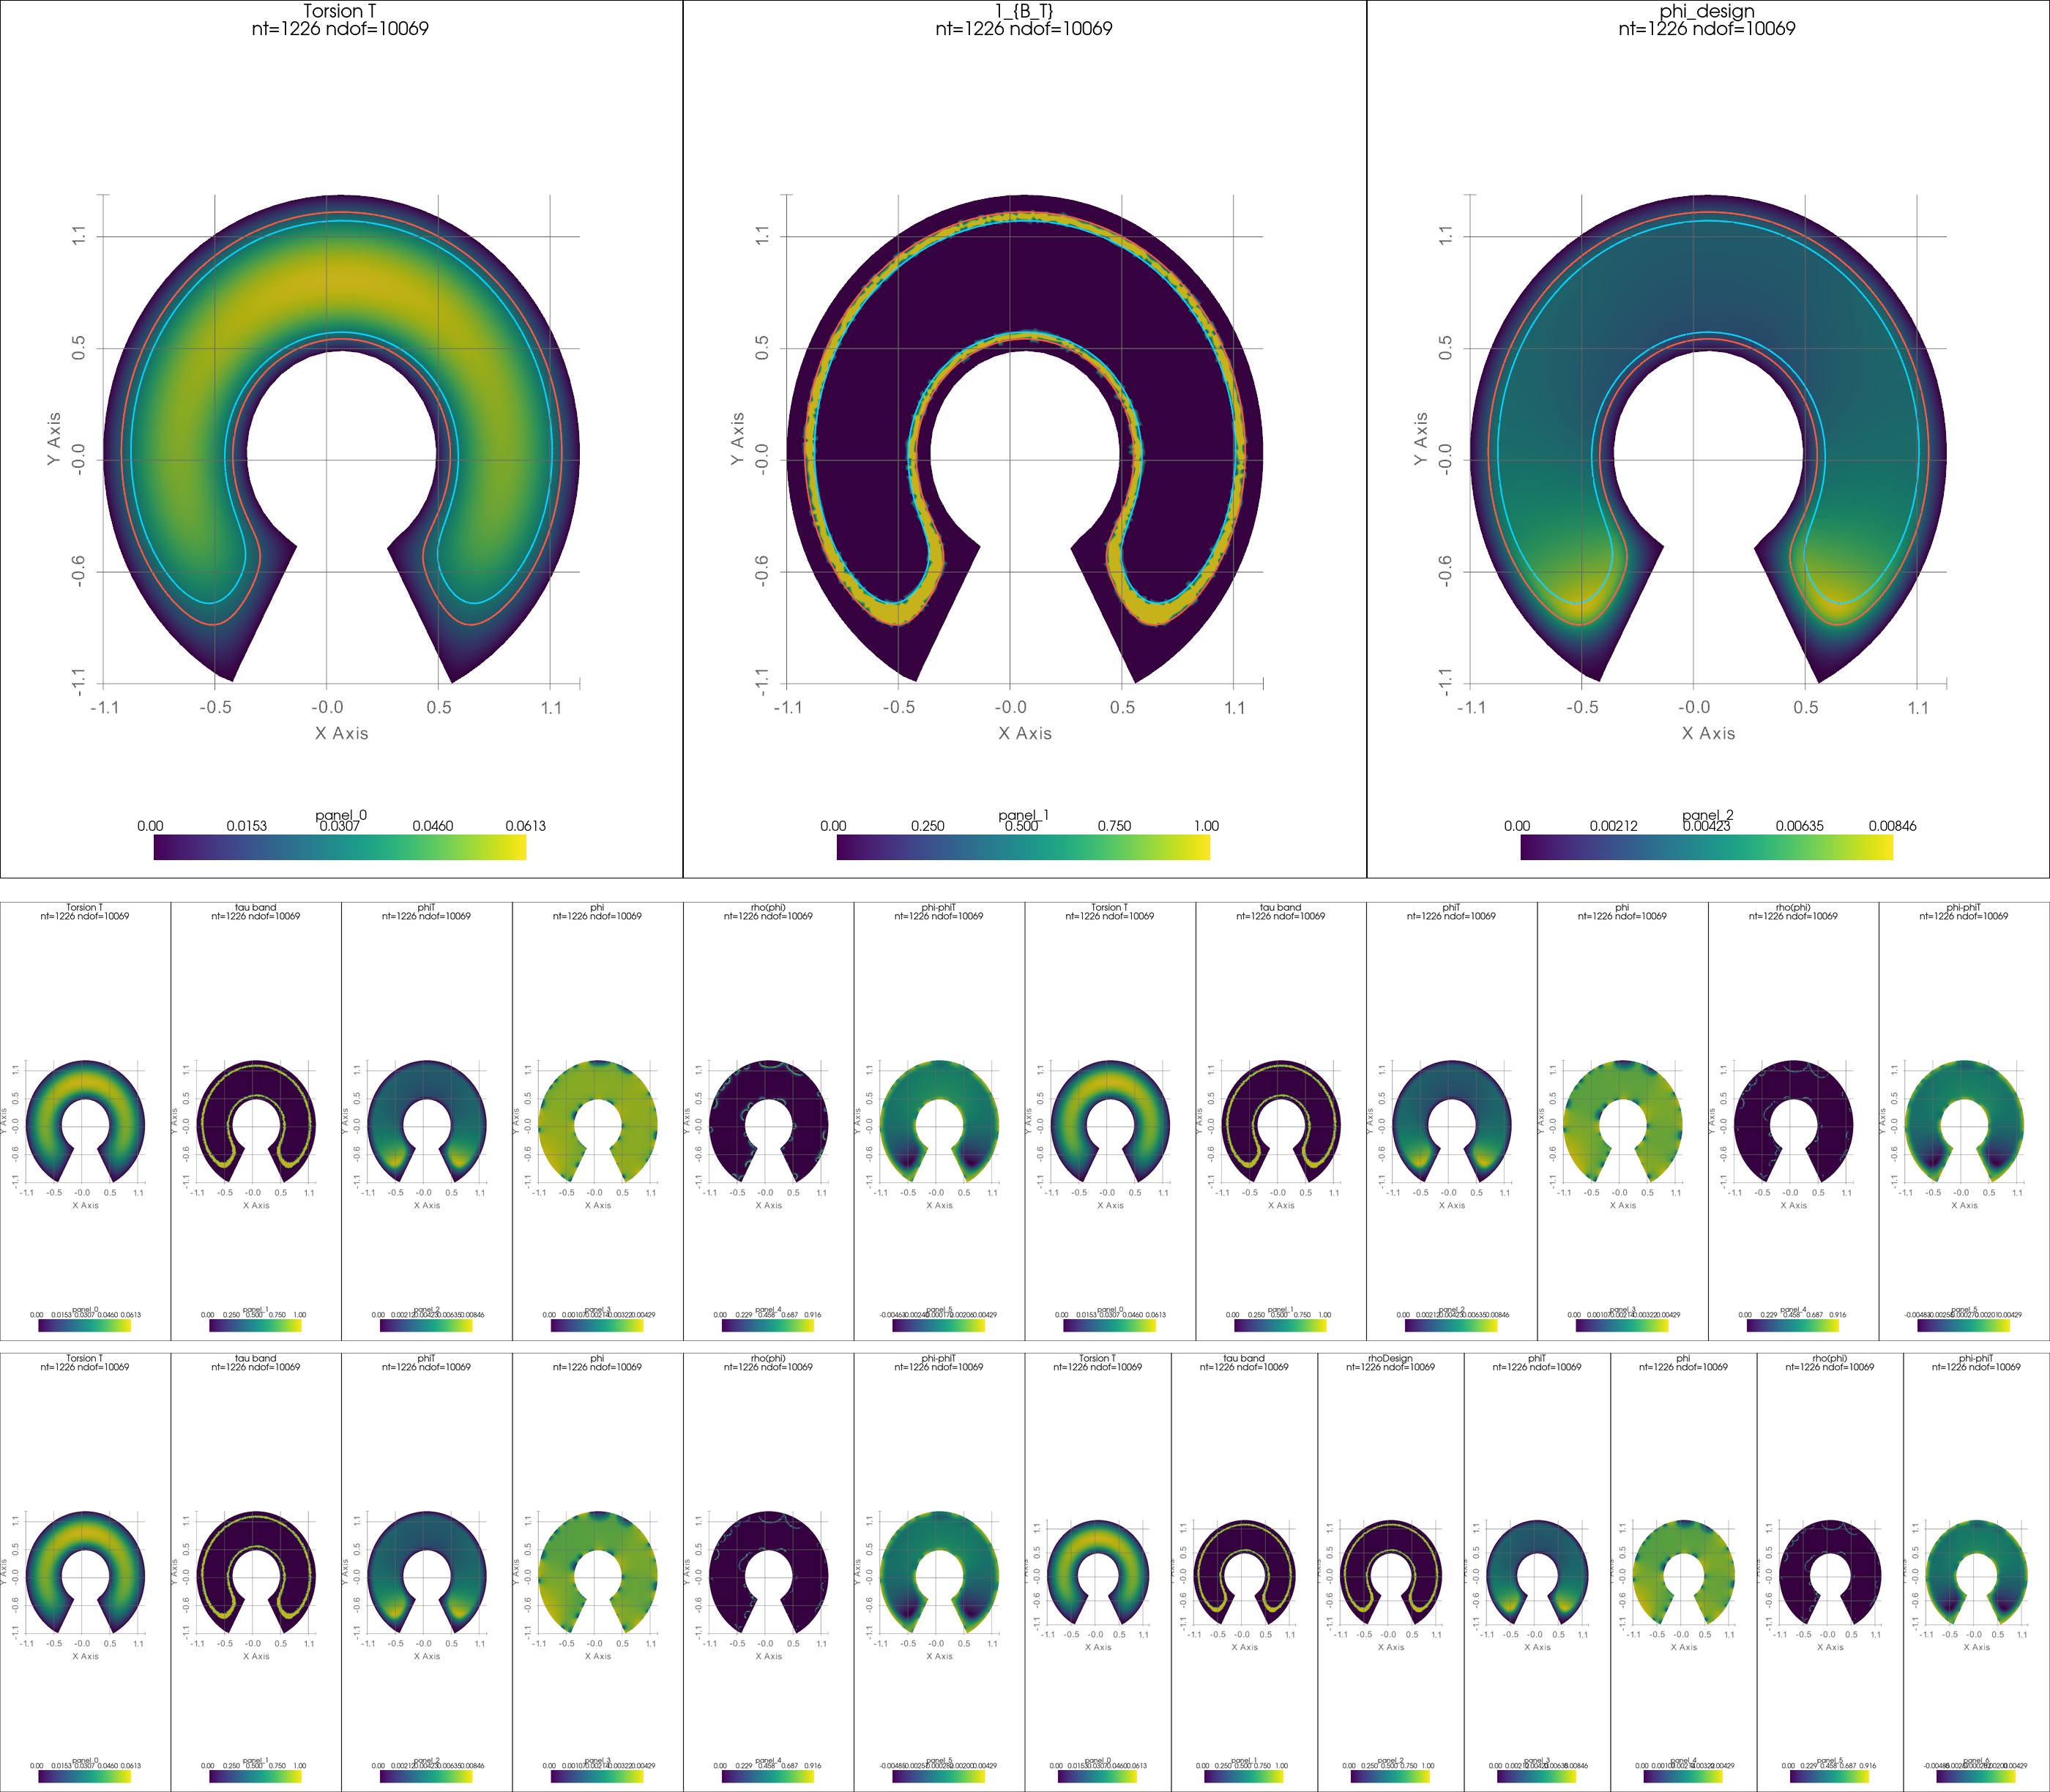
\includegraphics[width=\linewidth]{figures/horseshoe_0p35_0p50_adaptive_continuation_epsratio0160_weighted_l125_m100_storyboard.png}
\end{minipage}
\caption{Finite-merit retry.  Left: independently discovered adaptive-search
candidates and handoff.  Right: exact outer evolution, including the failed
terminal state.  Fixed torsion curves are dashed and equilibrium curves are
solid; fields are fully gathered on rank zero and the high-resolution mesh is
hidden.  All 157 individual candidate equilibria are retained as PNG files.
Data status: actual.}
\label{fig:horseshoe-weighted-storyboards}
\end{figure}
\end{landscape}

\subsection{Completion status}
\begin{tabular}{lr}
\toprule
Classification & Cases\\
\midrule
certified\_subband\_convergence & 27\\
deferred & 48\\
geometrically\_unsuccessful\_pde\_converged & 17\\
incomplete & 275\\
overview\_completed & 14\\
pde\_converged\_with\_capped\_trials & 3\\
pde\_failure & 46\\
stationarity\_completed & 5\\
strict\_convergence & 0\\
\bottomrule
\end{tabular}


\subsection{Limitations and unresolved cases}
The finest levels and extrapolated MUMPS rank choices must be measured before
claims of mesh independence or optimal scaling are made.  Cases lacking a
terminal state, a requested final PDE residual, or a decreasing two-grid
change are reported explicitly and are never silently omitted.
